\documentclass{MechThesis}
%
% Default options:
% [thesissizeG5,twoside,onecolumn,10pt,reqno,tbtags,globalpagenum,final]
%
%
% Available options:
% - size: [a4paper, letterpaper, thesissisze, thesissizeA4, thesissizeG5]
% - printing: [twoside, oneside]
% - columns: [onecolumn, twocolumns]
% - font size: [8pt, 9pt, 10pt, 11pt, 12pt]
% - position of equation numbers: [leqno, reqno]
% - split-equations numbers: [tbtags, centertags]
% - page numbers in papers: [globalpagenum, paperpagenum]
% - editing: [final, draft, printA4, cropmarks]
% - papers cover: [happyadvisor] (use it if you have more than 8 papers)
%
%
% Packages
%
% insert in this file any additional package
% Insert HERE any additional packages

\usepackage{graphicx} % Enhanced support for graphics

% Useful packages (not required):
%
% \usepackage{CJK} % CJK (Chinese, Japanese, Korean and Thai) language support
% \usepackage{listings} % Typeset source code listings using LaTeX
% \usepackage{longtable} % Allow tables to flow over page boundaries
% \usepackage{mathrsfs} % Support for using RSFS fonts in maths
% \usepackage{psfrag} % Replace strings in encapsulated PostScript figures
% \usepackage{rotating} % Rotation tools, including rotated full-page floats
% \usepackage{showframe} % Draw a page-layout diagram
% \usepackage[normalem]{ulem} % Package for underlining 

%===============================================================================
%                        DO NOT TOUCH WHAT FOLLOWS
%===============================================================================
%
% The following packages are required by the MechThesis class
%
\usepackage[utf8]{inputenc} % Accept different input encodings
\usepackage[swedish,english]{babel} % Multilingual support for Plain TeX or LaTeX
\usepackage{microtype} % Subliminal refinements towards typographical perfection
\usepackage{natbib} % Flexible bibliography support
\usepackage[hidelinks]{hyperref} % Extensive support for hypertext in LaTeX
\usepackage[margin=5pt,skip=0pt]{caption} % Correct figures and tables caption width
%\usepackage{natbib} % citep
%\usepackage{chapterbib} % multiple bibliographies
\usepackage[margin=5pt,skip=0pt]{subcaption}
\usepackage[shortlabels]{enumitem}
\usepackage{placeins}
\usepackage{wrapfig}
\usepackage{url}


%
% The following packages are loaded by MechThesis.cls and need not to be loaded
% in this file:
% - color
% - amsmath
% - amsfonts
% - amssymb
% - amsthm
% - amsgen
% - crop        (if [printA4] or [cropmarks] options are used)
% - fp          (if [happyadvisor] option is used)

%
%
% Commands
%
% insert in this file any additional command
% Insert HERE any additional commands


% as examples here are some commands from the JFM template:
%
\newcommand\etal{\mbox{\textit{et al.}}}
\newcommand\etc{etc.\ }
\newcommand\eg{e.g.\ }

\providecommand\bnabla{\boldsymbol{\nabla}}
\providecommand\bcdot{\boldsymbol{\cdot}}

\newcommand\Rey{\mbox{\textit{Re}}}  % Reynolds number
\newcommand\Pran{\mbox{\textit{Pr}}} % Prandtl number, cf TeX's \Pr product
\newcommand\Pen{\mbox{\textit{Pe}}}  % Peclet number
%%%%%%%%%%%%%%%%%%%%%%%%%%%%%%%%%%%%%%%%%%%%%%%%%%%%%%%%%%%%%%%%%%%%%%%%%%%%%%%
%
%   Symbols   Symbols   Symbols   Symbols   Symbols   Symbols   Symbols
%
%   (c) Copyright, 1985 by Moon J. Lee
%
%%%%%%%%%%%%%%%%%%%%%%%%%%%%%%%%%%%%%%%%%%%%%%%%%%%%%%%%%%%%%%%%%%%%%%%%%%%%%%%
%
\font\smallfont=cmsy10 at 10truept
\textfont8=\smallfont
\mathchardef\bigCircle="280D

\font\bigfont=cmsy10 at 14.4truept
\textfont9=\bigfont
\mathchardef\tiMes="2902        %

\font\Bigfont=cmsy10 at 17.28truept
\textfont10=\Bigfont
\mathchardef\DiaMond="2A05        %
%\mathchardef\buLlet="2A0F
\mathchardef\cirCle="2A0E
\mathchardef\BigCircle="2A0D

\font\Bbigfont=cmsy10 at 24.88truept
\textfont11=\Bbigfont
\mathchardef\buLLet="2B0F

%------------------------------------------------------------------------------%

\def\bigCirc{\raise 0.3ex\hbox{$\bigCircle$}\nobreak$\,$}
\def\Bigcirc{$\BigCircle$}                    %   very big circle (0.2" Diam.)
\def\Circ{\hbox{$\cirCle$}\nobreak$\,$}
\def\Bullet{\raise-0.35ex\hbox{$\buLLet$}\nobreak$\,$}
\def\triangleup{$\bigtriangleup$\nobreak$\,$}
\def\triangledown{\raise 0.2em\hbox{$\bigtriangledown$}\nobreak$\,$}
\def\uptriangle{\triangleup}       \def\downtriangle{\triangledown}
\def\Diamond{$\DiaMond$\nobreak$\,$}

\def\minisquare{\hbox{${\vcenter{
               \hrule height 0.3pt \kern-0.4pt
               \hbox{\vrule width  0.3pt height 3.0pt \kern 2.6pt
               \vrule width  0.3pt height 3.0pt} \kern-0.4pt
               \hrule height 0.3pt}}$}}
%\def\square{\raise 0.175ex\hbox{${\vcenter{
%               \hrule height 0.8truept       \kern-0.4truept
%               \hbox{\vrule width 0.8truept height 8.0truept \kern 7.6truept
%                     \vrule width 0.8truept height 8.0truept} \kern-0.4truept
%               \hrule height 0.8truept}}$}\nobreak$\,$}
\def\ssquare{\raise 0.175ex\hbox{${\vcenter{
               \hrule height 0.5truept       \kern-0.25truept
               \hbox{\vrule width 0.5truept height 3.0truept \kern 2.75truept
                     \vrule width 0.5truept height 3.0truept} \kern-0.25truept
               \hrule height 0.5truept}}$}\nobreak$\,$}
\def\squarex{\raise 0.175ex\hbox{${\vcenter{
               \hrule height 0.8truept       \kern-1.80truept
          \hbox{\vrule width 0.8truept height 8.0truept \kern-1.95truept
                \raise 0.8truept\hbox{$\tiMes$}     \kern-6.70truept
                \vrule width 0.8truept height 8.0truept} \kern-0.80truept
               \hrule height 0.8truept}}$}\nobreak$\,$}

\def\sqbull{\raise0.175ex\hbox{\vrule height 1.4ex width 1.6ex depth 0.2ex}\nobreak$\,$}
\def\smsqbull{\raise0.175ex\hbox{\vrule height 0.8ex width 0.9ex depth 0.2ex}\nobreak$\,$}

\def\Diamondplus{${\vcenter{\vcenter{\DiaMond} \kern-10truept
                            \hbox{\vrule width .4truept}\kern -3truept
                            \hrule height .4truept}}$\nobreak$\,$}
%
%%%%%%%%%%%%%%%%%%%%%%%%%%%%%%%%%%%%%%%%%%%%%%%%%%%%%%%%%%%%%%%%%%%%%%%%%%%%%%%
%
%         Lines   Lines   Lines   Lines   Lines   Lines   Lines
%
%%%%%%%%%%%%%%%%%%%%%%%%%%%%%%%%%%%%%%%%%%%%%%%%%%%%%%%%%%%%%%%%%%%%%%%%%%%%%%%
\newcount\ndots

\def\drawline#1#2{\raise 2.5truept\vbox{\hrule width #1truept height #2truept}}
\def\moonspace#1{\hskip #1truept}

\def\shortchain{\drawline{6.0}{0.75}}     
\def\chain{\drawline{12.0}{0.75}}     
\def\thinchain{\drawline{12.0}{0.25}}     
\def\chainspace{\chain\moonspace{2}}
\def\shortchainspace{\shortchain\moonspace{2}}
\def\thinchainspace{\thinchain\moonspace{2}}
\def\Dashy{\drawline{4.00}{1.00}}     
\def\dashy{\drawline{4.00}{0.75}}     
\def\thindashy{\drawline{4.00}{0.25}}     
\def\dashyspace{\dashy\moonspace{2}}
\def\Dashyspace{\Dashy\moonspace{2}}
\def\thindashyspace{\thindashy\moonspace{2}}
\def\longdashy{\drawline{8.00}{0.75}} 
\def\thinlongdashy{\drawline{8.00}{0.25}} 
\def\longdashyspace{\longdashy\moonspace{2}}
\def\thinlongdashyspace{\thinlongdashy\moonspace{2}}
\def\Dotty{\drawline{1.00}{1.00}}     
\def\dotty{\drawline{1.00}{0.75}}     
\def\thindotty{\drawline{1.00}{0.25}}     
\def\Dottyspace{\Dotty\moonspace{2}}
\def\dottyspace{\dotty\moonspace{2}}
\def\thindottyspace{\thindotty\moonspace{2}}

\def\solid{\drawline{24}{0.75}\nobreak$\,$}  
\def\Solid{\drawline{24}{1.00}\nobreak$\,$}  
\def\thinsolid{\drawline{24}{0.25}\nobreak$\,$}  
\def\circthinsolid{$\circ$\drawline{6}{0.25}$\circ$\drawline{6}{0.25}$\circ$\nobreak$\,$}  

\def\circthinsolidpict{\begin{picture}(10,2)\linethickness{0.5pt}\put(0,1){\circle{3}}\put(0.5,1){\line(1,0){3}}\put(3.8,1){\circle{3}}\put(4.5,1){\line(1,0){3}}\put(7.8,1){\circle{3}}\end{picture}}  

\def\thinsolidpict{\begin{picture}(10,2)\linethickness{0.5pt}\put(0,1){\line(1,0){8}}\end{picture}}  

\def\thicksolidpict{\begin{picture}(10,2)\linethickness{1pt}\put(0,1){\line(1,0){8}}\end{picture}} 

\def\thindashedpict{\begin{picture}(11,2)\linethickness{0.5pt}\put(0,1){\line(1,0){2}}\put(2.5,1){\line(1,0){2}}\put(5,1){\line(1,0){2}}\put(7.5,1){\line(1,0){2}}\end{picture}}  

\def\dashedpict{\begin{picture}(11,2)\linethickness{0.75pt}\put(0,1){\line(1,0){2}}\put(2.5,1){\line(1,0){2}}\put(5,1){\line(1,0){2}}\put(7.5,1){\line(1,0){2}}\end{picture}}  

\def\squarethinsolidpict{\begin{picture}(10,2)\linethickness{0.5pt}\put(0,0.3){{\tiny $\square$}}\put(1.5,1){\line(1,0){2}}\put(3.3,0.3){{\tiny $\square$}}\put(4.7,1){\line(1,0){2}}\put(6.3,0.3){{\tiny $\square$}}\end{picture}}  

\def\diamondthinsolidpict{\begin{picture}(10,2)\linethickness{0.5pt}\put(0,0.3){{\small $\diamond$}}\put(1.5,1){\line(1,0){2}}\put(3.3,0.3){{\small $\diamond$}}\put(4.7,1){\line(1,0){2}}\put(6.3,0.3){{\small $\diamond$}}\end{picture}}  

%  ---------------------------

\def\thindotbox{\hbox{\thindottyspace}}
\def\Dotbox{\hbox{\Dottyspace}}
\def\dotbox{\hbox{\dottyspace}}
\def\Dotted{\hbox{\leaders\Dotbox\hskip 24truept}\nobreak$\,$}  
\def\thindotted{\hbox{\leaders\thindotbox\hskip 24truept}\nobreak$\,$}  
\def\dotted{\hbox{\leaders\dotbox\hskip 24truept}\nobreak$\,$}  
%  .  .  .  .  .  .  .  .  .  .

\def\dashbox{\hbox{\dashyspace}}  
\def\Dashbox{\hbox{\Dashyspace}}  
\def\dashed{\hbox {\ndots=0 \loop\ifnum\ndots<3\advance\ndots by 1
        \dashbox\repeat\dashy}\nobreak$\,$}       
\def\Dashed{\hbox {\ndots=0 \loop\ifnum\ndots<3\advance\ndots by 1
        \Dashbox\repeat\Dashy}\nobreak$\,$}       
\def\thindashbox{\hbox{\thindashyspace}}  
\def\thindashed{\hbox {\ndots=0 \loop\ifnum\ndots<3\advance\ndots by 1
        \thindashbox\repeat\thindashy}\nobreak$\,$}       
\def\thindash{\hbox {\ndots=0 \loop\ifnum\ndots<3\advance\ndots by 1
        \thindashbox\repeat\thindashy}\nobreak$\,$}       
%   --  --  --  --  --  --  --

\def\longdashbox{\hbox{\longdashyspace}}  
\def\thinlongdashbox{\hbox{\thinlongdashyspace}}  
\def\longdash{\hbox {\ndots=0 \loop\ifnum\ndots<3\advance\ndots by 1
        \longdashbox\repeat\longdashy}\nobreak$\,$}       
\def\thinlongdash{\hbox {\ndots=0 \loop\ifnum\ndots<3\advance\ndots by 1
        \thinlongdashbox\repeat\thinlongdashy}\nobreak$\,$}       
%   ----  ----  ----  ----  ----  

\def\chndot{\hbox{\chainspace\dottyspace\chain}\nobreak$\,$}   
\def\dotdashed{\hbox{\shortchainspace\dottyspace\shortchain}\nobreak$\,$}      
%   ----  .  ----  .  ----

\def\chndash{\hbox{\chainspace\dashyspace\chain}\nobreak$\,$}      
\def\thinchndash{\hbox{\thinchainspace\thindashyspace\thinchain}\nobreak$\,$}      
%   ----  --  ----  --  ----

\def\chndashdash{\hbox{\chainspace\dashyspace\dashyspace\chain}\nobreak$\,$}
%   ----  --  ----  --  ----

\def\dotdashdash{\hbox{\dottyspace\dashyspace\dashyspace\dottyspace}\nobreak$\,$}
%   ----  --  ----  --  ----

\def\chndotdot{\hbox{\chainspace\dottyspace\dottyspace\chain}\nobreak$\,$}
%   ----  .  .  ----  .  .  ----  

\def\chndotdotdot{\hbox{\chainspace\dottyspace\dottyspace\dottyspace\chain}\nobreak$\,$}
%   ----  .  .  .  ----  .  .  .  ----  

\def\longdot{\hbox{\drawline{2}{.5}\moonspace{2}}}

\def\longdots{\hbox{\leaders\longdot\hskip 24truept}\nobreak$\,$}

\def\Longdot{\hbox{\drawline{3}{.5}\moonspace{2}}}

\def\Longdots{\hbox{\leaders\Longdot\hskip 24truept}\nobreak$\,$}





%-------------------------------------------------------------------------------
% Thesis information
%-------------------------------------------------------------------------------
%
\title[Boundary layers over wing sections]% Title used in the abstract (optional)
{% Title of the thesis
	Boundary layers over \\ wing sections
}%

\author{Prabal S. Negi}% Author

\affiliation
{%	Author's affiliation
%	Linn\'e FLOW Centre, KTH Mechanics, Royal Institute of Technology\\
%	SE-100 44 Stockholm, Sweden%
	Department of Mechanics, Linn\'e FLOW Centre and Swedish e-Science Research Centre (SeRC),
	KTH Royal Institute of Technology, \\
	SE-100 44 Stockholm, Sweden
}%

\titel
{% Swedish title (for swedish abstract)
	Gr\"{a}nsskikt \"{o}ver vingsektioner
}%

\anslutning
{% Author's swedish affiliation (for swedish abstract)
	Institutionen för Mekanik, Linn\'e FLOW Centre and Swedish e-Science Research Centre (SeRC),
	Kungliga Tekniska H\"ogskolan\\
	SE-100 44 Stockholm, Sverige%
}%

\date{Stockholm}{December}{2017}% City, Month, Year

\info{% Defence information (in swedish)
	Akademisk avhandling som med tillst\aa nd av Kungliga Tekniska H\"{o}gskolan
	i Stockholm framl\"{a}gges till offentlig granskning f\"{o}r avl\"{a}ggande
	av teknologie
	doktorsexamen % doctorsexamen/licentiatsexamen
	\"{o}nsdagen den 13 December 2017 kl 15:15 % day
	i sal D3, % room
	Kungliga Tekniska H\"{o}gskolan, Lindstedtsv\"{a}gen 5, Stockholm.% address
	%
	\\[\baselineskip]% Publishing info
	%	
	TRITA-MEK Technical report 2017:15\\
	ISSN 0348-467X\\
	ISRN KTH/MEK/TR-17/15-SE\\
	ISBN 978-91-7729-591-4
	%
	\\[\baselineskip]% Cover info (comment if no cover image is used)
	%
	%{\it Cover:} schematics of a thermal exhaust port of the Death Star.
}%

\printer{Universitetsservice US--AB, Stockholm}% Printer informations


%===============================================================================
%===============================================================================
%                            BEGIN DOCUMENT
%===============================================================================
%===============================================================================

%\includeonly{overview}

\begin{document}


%===============================================================================
% Frontmatter
%===============================================================================
%
\frontmatter

%-------------------------------------------------------------------------------
% Cover page
%-------------------------------------------------------------------------------
%
\makecoverpage


%-------------------------------------------------------------------------------
% Dedication (comment if none)
%-------------------------------------------------------------------------------
%
\dedication{
	\begin{minipage}[r]{0.75\textwidth}
		{\it ``His reading suggested a man swimming in the sea among the wreckage of his ship,
		and trying to save his life by greedily clutching first at one spar and then at another.''}\\ [5pt]
		\begin{flushright}
			- Anton Chekhov \\
			The Bet
		\end{flushright}
	\end{minipage}
}


%-------------------------------------------------------------------------------
% Abstract (English)
%-------------------------------------------------------------------------------
%
\begin{abstract}
	The understanding of developing boundary layers over wings is an important topic from the perspective of industrial applications. An increased understanding would be consequential not only for achieving higher fuel efficiency but also in the design of aircraft control strategies. With these aims in mind, the current work aims to further the understanding of developing boundary layer over wing sections. The study is performed with two particular perspectives in mind - unsteady aerodynamic effects in a pitching airfoil and turbulent boundary layer structure in non-equilibrium boundary layers over a stationary airfoil.
	
	The boundary layer evolution in unsteady natural laminar flow airfoils undergoing small-amplitude pitch-oscillations is investigated. For high Reynolds numbers the origins of the non-linear unsteady aerodynamic response of laminar airfoils is explained on the basis of quasi-steady assumptions. Temporal non-linearities in aerodynamic forces are shown to be inherently linked to the non-linearities of static aerodynamic force coefficients and that a simple phase-lag concept can model the observed non-linear unsteady response. On the other hand at lower Reynolds numbers, when there exists an unstable leading-edge laminar separation bubble, the unsteady response is dynamically rich and changes in boundary layer characteristics can be abrupt. The quasi-steady phase-lag concepts are no longer appropriate to explain the unsteady flow physics in such a case.
	
	For the case of stationary airfoils, flow statistics for flow around an airfoil at two different Reynolds numbers are compared to assess Reynolds number effects in non-equilibrium flows. Pressure gradient effects are found to be stronger at low Reynolds numbers, leading to higher energy in the larger structures present in the outer part of the turbulent boundary layer. 
	
        \keywords{boundary layers, unsteady aerodynamics, non-equilibrium flows}
        %
\end{abstract}


%-------------------------------------------------------------------------------
% Abstrakt (Swedish) 
%-------------------------------------------------------------------------------
%
\begin{abstrakt}
	Förståelsen av det strömningsmekaniska gränsskiktet som utvecklas över vingar är av stort intresse för industriella tillämpningar. En ökad förståelse av detta är ett måste både för att uppnå en minskning av bränsleförbrukning och för för utformningen av effektivare flygstyrsystem. Med detta i åtanke, syftar detta arbetet till att vidga vår förståelse av det komplexa gränsskiktetsflödet över vingar. Studien utförs med två specifika mål i åtanke - instationära aerodynamiska effekter i strömningen över en oscillerande vinge och strukturer i ett turbulent gränsskikt över en stationär vinge som inte är i jämvikt.
	
	Här har vi studerat utvecklingen av ett instationär gränsskikt över en vinge designad för att ha laminär flöde (så kallade NLF vinge). Vingen genomgår oscillationer med små amplituder. För höga Reynoldstal förklaras ursprunget till det ickelinjära aerodynamiska responsen hos NLF vingar genom antagandet av kvasistationär strömning. Tidsberoende ickelinjäriteter hos de aerodynamiska krafterna visar sig vara starkt kopplade till de ickelinjäriteter hos de statiska aerodynamiska kraftkoefficienterna och med hjälp av ett enkelt fasfördröjningskoncept kan man modellera den observerade ickelinjära instationära responsen. Å andra sidan, vid lägre Reynoldstal, när det finns en instabil laminär separationsbubbla vid framkanten av vingen, visar den instationära responsen en stark dynamik och förändringar i karaktären av gränsskiktet kan vara abrupta. I sådana fall är antagandet av en kvasistationär fasfördröjning inte längre adekvat för att förklara fysiken hos det instationära flödet.
	
	I fallet med den stationärs vingen jämför vi flödesstatistiken vid två olika Reynoldstal för att förstå effekter av detta för turbulenta flöden som befinner sig i ickejämvikt. Tryckgradientenseffekter visade sig vara starkare vid låga Reynoldstal, vilket leder till högre energi i de större strukturerna som är närvarande i den yttre delen av det turbulenta gränsskiktet.
    %
    \nyckelord{gränsskikt, ostabil aerodynamik, icke-jämviktsflöden}
    %
\end{abstrakt}


%-------------------------------------------------------------------------------
% Preface page
%-------------------------------------------------------------------------------
%
\begin{preface}
	This thesis deals with boundary layers developing over a wing section. A brief introduction of the basic concepts and methods is presented in the first part. The second part contains four articles. The first two are internal technical reports. The third paper is an extended version of the paper presented at the $10^{th}$ International Symposium on Turbulence \& Shear Flow Phenomenon (TSFP-10), Chicago, USA. The final paper was also presented at TSFP-10. The fourth paper has been adjusted to comply with the present thesis format for consistency, but the contents have not been altered as compared with the original counterpart, except for the addition of an appendix.
\end{preface}


%-------------------------------------------------------------------------------
% Division of work between authors
%-------------------------------------------------------------------------------
%
\begin{divisionofwork}
	The main advisor for the project is Professor Dan S. Henningson (DH).
	Docent Ardeshir Hanifi (AH) and Assoc.\ Professor Philipp Schlatter (PS) act as co-advisor.

	\paperitem
		The matlab code has been developed by Prabal S. Negi (PSN). The numerical simulations have been set-up and run by PSN. The paper has been written by PSN with feedback from PS and DH. 

	\paperitem
		The numerical simulation has been set-up and run by PSN. The paper has been written by PSN with feedback from AH and DH. 

	\paperitem
		The numerical simulations for channel flows and pitching airfoil have been set-up and run by PSN. Numerical simulations for LES validation on wing section was setup by PSN and run by Ricardo Vinuesa (RV). The paper has been written by PSN with feedback from RV, AH, PS and DH. 

	\paperitem
		The numerical simulation for the $Re_{c}=1,000,000$ case has been set-up by PSN and run by RV. The domain validation was performed by PSN. The paper has been written by RV with feedback from PSN, AH, DH and PS.

\end{divisionofwork}


%-------------------------------------------------------------------------------
% Additional publications (comment if none)
%-------------------------------------------------------------------------------
%
%\begin{otherpublications}
%	The following papers, although related, are not included in this thesis.
%
%  \paperitem%
%    {Anakin Skywalker \& Master Obi-Wan Kenobi}% Authors
%    {3639}% Year
%    {The light sabre: an elegant weapon for a more civilized age}% Title
%    {Jedi Journal of Weapons}% Journal
%    {33}% Volume
%    {2}% Number
%    {pp. 55--60}% Pages

%\end{otherpublications}


%-------------------------------------------------------------------------------
% Conferences (comment if none)
%-------------------------------------------------------------------------------
%
\begin{conferences}
	Part of the work in this thesis has been presented at the following 
	international conferences. The presenting author is underlined.

  \conferenceitem%
  {\underline{P. S. Negi}, R. Vinuesa, A. Hanifi, P. Schlatter \& D. S. Henningson}% Authors
  {2017}% Year
  {Large-eddy simulations of a wing section undergoing small-amplitude pitch oscillations}% Title
  {$16^{th}$ European Turbulence Conference (ETC)}% Conference
  {Stockholm, Sweden}% Location


  \conferenceitem%
  {\underline{P. S. Negi}, R. Vinuesa, A. Hanifi, P. Schlatter \& D. S. Henningson}% Authors
  {2017}% Year
  {Unsteady Aerodynamic effects in small-amplitude pitch oscillations of an airfoil}% Title
  {$10^{th}$ Int. Sym. on Turbulence \& Shear Flow Phenomenon (TSFP-10)}% Conference
  {Chicago, USA}% Location

  \conferenceitem%
  {\underline{R. Vinuesa}, P. S. Negi, A. Hanifi, D. S. Henningson \& P. Schlatter}% Authors
  {2017}% Year
  {High-fidelity simulations of the flow around wings at high Reynolds numbers}% Title
  {$10^{th}$ Int. Sym. on Turbulence \& Shear Flow Phenomenon (TSFP-10)}% Conference
  {Chicago, USA}% Location
  
  \conferenceitem%
  {\underline{P. S. Negi}, R. Vinuesa, P. Schlatter, A. Hanifi, \& D. S. Henningson}% Authors
  {2016}% Year
  {Relaxation-term filertering for SEM}% Title
  {$5^{th}$ Nek user's meeting}% Conference
  {Cambridge, USA}% Location  

\end{conferences}


%-------------------------------------------------------------------------------
% Table of contents
%-------------------------------------------------------------------------------
%
\tableofcontents



%===============================================================================
% Part I: Overview and summary
%===============================================================================
%
\mainmatter

\part{Overview and summary}

%-------------------------------------------------------------------------------
% Overview and summary
%
\graphicspath{{imgs/}}
%\setlength{\captionmargin}{50pt}

%===============================================================================
\chapter{Introduction}
%===============================================================================
\section{A short history}

The first sustained flight by the Wright brothers in 1903 marked a historic day in human achievement and ingenuity. Momentous as the achievement was, the Wright brothers did not truly invent the modern airplane. Their achievements were the fruition of nearly a century of aeronautical research, starting perhaps with Sir George Cayley, who is considered the ``father of aerial navigation'' \citep{gibbs-smith62}. The principal components of the modern aircraft were laid down by George Cayley as early as 1799. Prior to Cayley, the ideas for mechanical flight tended towards flapping wings, where the flapping motion produced both propulsion and lift. George Cayley was the first to break the unsuccessful chain of thought and separated the two aspects of flight into distinct systems. His triple paper ``On Aerial Navigation'' published in Nicholason's \textit{Journal of Natural Philosophy, Chemistry and the Arts} on November 1809, February and March 1810 \citep{cayley1809} mark some of the most important works in aeronautical history. In the works, Cayley states for the first time, the principle of lift generation \textit{i.e.} the formation of a low pressure region on the upper surface of the wing. His paper elaborates on the separation of lift from propulsion and also goes on to talk about flight control and airplane stability. Later in his life, he proposed the concept of multiplanes (multiple wings mounted on top of each other) and built the first glider triplane named the ``boy carrier'' in 1849.

Several investigators followed the quest of ``aerial navigation''. Otto Lilienthal was the first to design and successfully fly controlled gliders in 1891, going on to make over $2500$ successful glider flights. Octave Chanute brought aeronautics research to America and designed a biplane glider which directly inspired the designs of the Wright Brothers. Samuel Pierpont Langley was a contemporary of the Wright brothers who built and tested several powered model airplanes. His success in achieving powered flight directly influenced and encouraged the Wright brothers. The final historic achievement of successful powered flight was achieved by the Wright brothers. On December $17^{th}$ 1903, a gasoline powered biplane by the name Wright Flyer I (figure~\ref{fig:wright_flight}) took flight in (modern day) Kill Devil Hills, North Carolina, ushering forth the era of practical human flight.
\begin{figure}[h]
	\centering
	\includegraphics[width=0.90\textwidth]{wright_brothers_first_flight}
	\vspace{10pt}	
	\caption{First flight of the Wright Flyer I, December 17, 1903, Orville piloting, Wilbur running at wingtip. Image from \cite{wikipedia_wright}.}
	\label{fig:wright_flight}
\end{figure}

\section{Modern aircraft design}
Since that fateful day, modern airplanes have been used in a variety of different conditions, varying from commercial passenger planes, to supersonic military aircrafts \citep{blackbird}, 
to endurance flights around the world lasting 9 days \citep{rutan_voyager}. The myriad uses have resulted in various challenges that need to be overcome by the aircraft designers. One significant challenge has been due to the dynamic interaction of air flow with the airplane structures, now studied under the field of aeroelasticity. These problems came to the fore as the design speed of aircrafts increased over the years and designers came to favor monoplanes over the biplane design. An early example was that of the Fokker D-8 German aircraft during World War I which suffered wing failure under steep dives, which was the first documented case of static aeroelastic effects.

Today the designers of commercial aircrafts face another challenge brought about by global climate change and rising oil prices. With the realization of the contribution of the aviation industry towards global climate change \citep{green08}, aircraft designers now face a need to significantly improve the fuel efficiency of commercial aircrafts in a bid to reduce the carbon footprint of the industry. In an effort to quantify the opportunities of achieving such an improvement, \cite{schrauf05} showed a break-down of the drag experienced by a typical transport aircraft highlighting that frictional drag accounted for more than half the drag experienced by the aircraft. Clearly a favorable modulation of the boundary layer over the wing could help achieve large improvements in fuel efficiency. The modulation could come in the form of effective flow control strategies, or with wing design strategies such as the use of natural laminar flow (NLF) airfoils. Both \cite{schrauf05} and \cite{green08} push forward the idea that NLF airfoils and laminar flow control strategies are the low-hanging fruits in the goal of higher fuel efficiency and a concerted effort into addressing the engineering challenges for practical implementation must be made. Some of these challenges may require revisiting the aeroelasticity problems from the perspective of laminar wings. However laminar flow at high Reynolds numbers is susceptible to destabilization and may not always be possible. Thus turbulent drag reduction strategies need to be used effectively where needed \citep{bushnell03}. Whatever the form of drag reduction technique that may finally be implemented on a particular aircraft, the understanding of developing boundary layers over wings (including the influence of control strategies) occupies a central position in aerodynamic research if the goal of higher fuel efficiency is to be realized. With this goal in mind, the current thesis work aims to further the understanding of developing boundary layers over airplane wings, focusing on two particular aspects.
\begin{itemize}
	\item Understanding the structure of the turbulent boundary layer developing over a wing section.	
	\item Understanding the evolution of the developing boundary layer over a natural laminar flow airfoil in unsteady flight conditions. 
\end{itemize}

%Solutions to these emerging aeroelastic problems needed an understanding of the unsteady phenomenon occurring in practical flight conditions. Such understanding came via the works of \cite{glauert30,karman38,theodorsen35} \textit{etc}, and by the 1940s, design engineers had the tools to account for unsteady aeroelastic effects in their wing designs.

%The achievements of these early aerdynamicists is quite impressive in particular considering that the boundary layer concept was in its nascent stages when the first practical airplanes were being designed. Indeed Prandtl's revolutionary concept of a boundary layer was first presented in 1904, almost a full year after the first flight of the Wright brothers.  

%-------------------------------------------------------------------------------
\section{Boundary layers over a stationary wing}

The understanding of the structure and scaling of wall-bounded turbulent flows has been in study for several decades and a complete understanding still remains far from complete. These flows have been studied with different canonical geometries such as channels \citep{kim87,moser99,lee15}, pipes \citep{elkhoury13,jimenez08,chin15} and flat plates \cite{spalart88,schlatter10,eitel14}. For the case of spatially evolving boundary layers over a flat plate, the simplest canonical case involves boundary-layer evolution subjected to a zero pressure gradient (ZPG). These flows may be uniquely characterized by a single parameter, \textit{i.e.} the Reynolds number Re, which is the ratio of the inertial and viscous scales of the flow. However practical flow cases are often influenced by pressure gradients. Such flow cases can no longer be uniquely defined using a single parameter. \cite{clauser54} with intuitive reasoning proposed a concept of an equilibrium boundary layer which may be uniquely defined by two parameters. He argued that, if the ratio of the average pressure gradient force across the boundary layer and the viscous shear force at the wall remains constant, the boundary layer would experience a similar flow history throughout its evolution. Thus the equilibrium pressure gradient boundary layers are uniquely defined by two parameters, namely the Reynolds number (Re) and the pressure gradient parameter $\beta$, defined as
\begin{eqnarray}
	\beta = \delta^{*}(dp/dx)/\tau_{w},
\end{eqnarray}
where $\delta^{*}$ is the displacement thickness, $dp/dx$ is the pressure gradient and $\tau_{w}$ is the wall-shear stress. The parameter is commonly referred to as the Clauser parameter. A flow case with a spatially constant Clauser parameter is categorized as an equilibrium boundary layer and a ZPG boundary layer is a special case of an equilibrium boundary layer with $\beta=0$. Several works have focused on pressure gradient boundary layers ranging from theoretical studies by \cite{townsend56,townsend56b,mellor66}, experimental works of \cite{skare94,harun13} and numerical simulations by \cite{spalart93,skote98}. The developing boundary layer over an airfoil however further increases in complexity since these boundary layers fall under the category of non-equilibrium boundary layers where the Clauser parameter is spatially varying. In such cases the flow history also plays a role in determining the local boundary layer properties \citep{clauser54,bobke17}. Analysis of such flow cases becomes significantly more difficult since the local boundary layer parameters do not uniquely define the state of the boundary layer. Nonetheless the study of such boundary layers is important since generic boundary layers found in nature would belong to this category, including the boundary layers over wings. The boundary layer developing over the NACA 4412 airfoil has the property that the spatially varying Clauser parameter is insensitive to Reynolds number. The presents us with the opportunity to study the Reynolds number effects of a non-equilibrium boundary layer with a constant pressure gradient history. That is indeed the methodology followed in this work. The developing boundary layer over a NACA 4412 wing section is analyzed at two different Reynolds numbers in order to understand Reynolds number effects in non-equilibrium boundary layers.

\section{Unsteady boundary layers}
%
Unsteady aeroydnamic studies started with the emergence of aeroelastic phenomenon in the early part of the $20^{th}$ century. With the gradual shift to monoplane designs, the inherent high torsional stiffness of biplanes was lost and aerodynamic instabilities, such as the one experienced by the Fokker D-8 became important. Pioneering works of \cite{glauert30,karman38,theodorsen35} \textit{etc}, provided the insight and modeling of such unsteady aerodynamic behavior and by the 1940s the foundations of unsteady aerodynamics for incompressible attached flows had been laid down. The mathematical framework these unsteady aerodynamic theories relied on simple inviscid and quasi-steady assumptions, which proved to be highly attractive to the wing designers \citep{leishman00}. Experimental corroboration by \cite{halfman52} and \cite{rainey57} further added support to the validity of the simple assumptions. Over the next few decades, investigations of unsteady aerodynamics shifted focus to the understanding of the dynamic stall phenomenon, with works of \cite{mccroskey76,mccroskey81,mccroskey82experimental,mccroskey82,carr1977,crisler94}. A large body of work on unsteady separated flows was presented by \cite{ericsson86,ericsson87b,ericsson_stall88a,ericsson_stall88b}. The studies continue to this day with the works of \cite{visbal11,visbal14,visbal17,dunne2015} and several other authors, a recent review can be found in \cite{coorke15}. 
\begin{figure}[h]
	\centering
	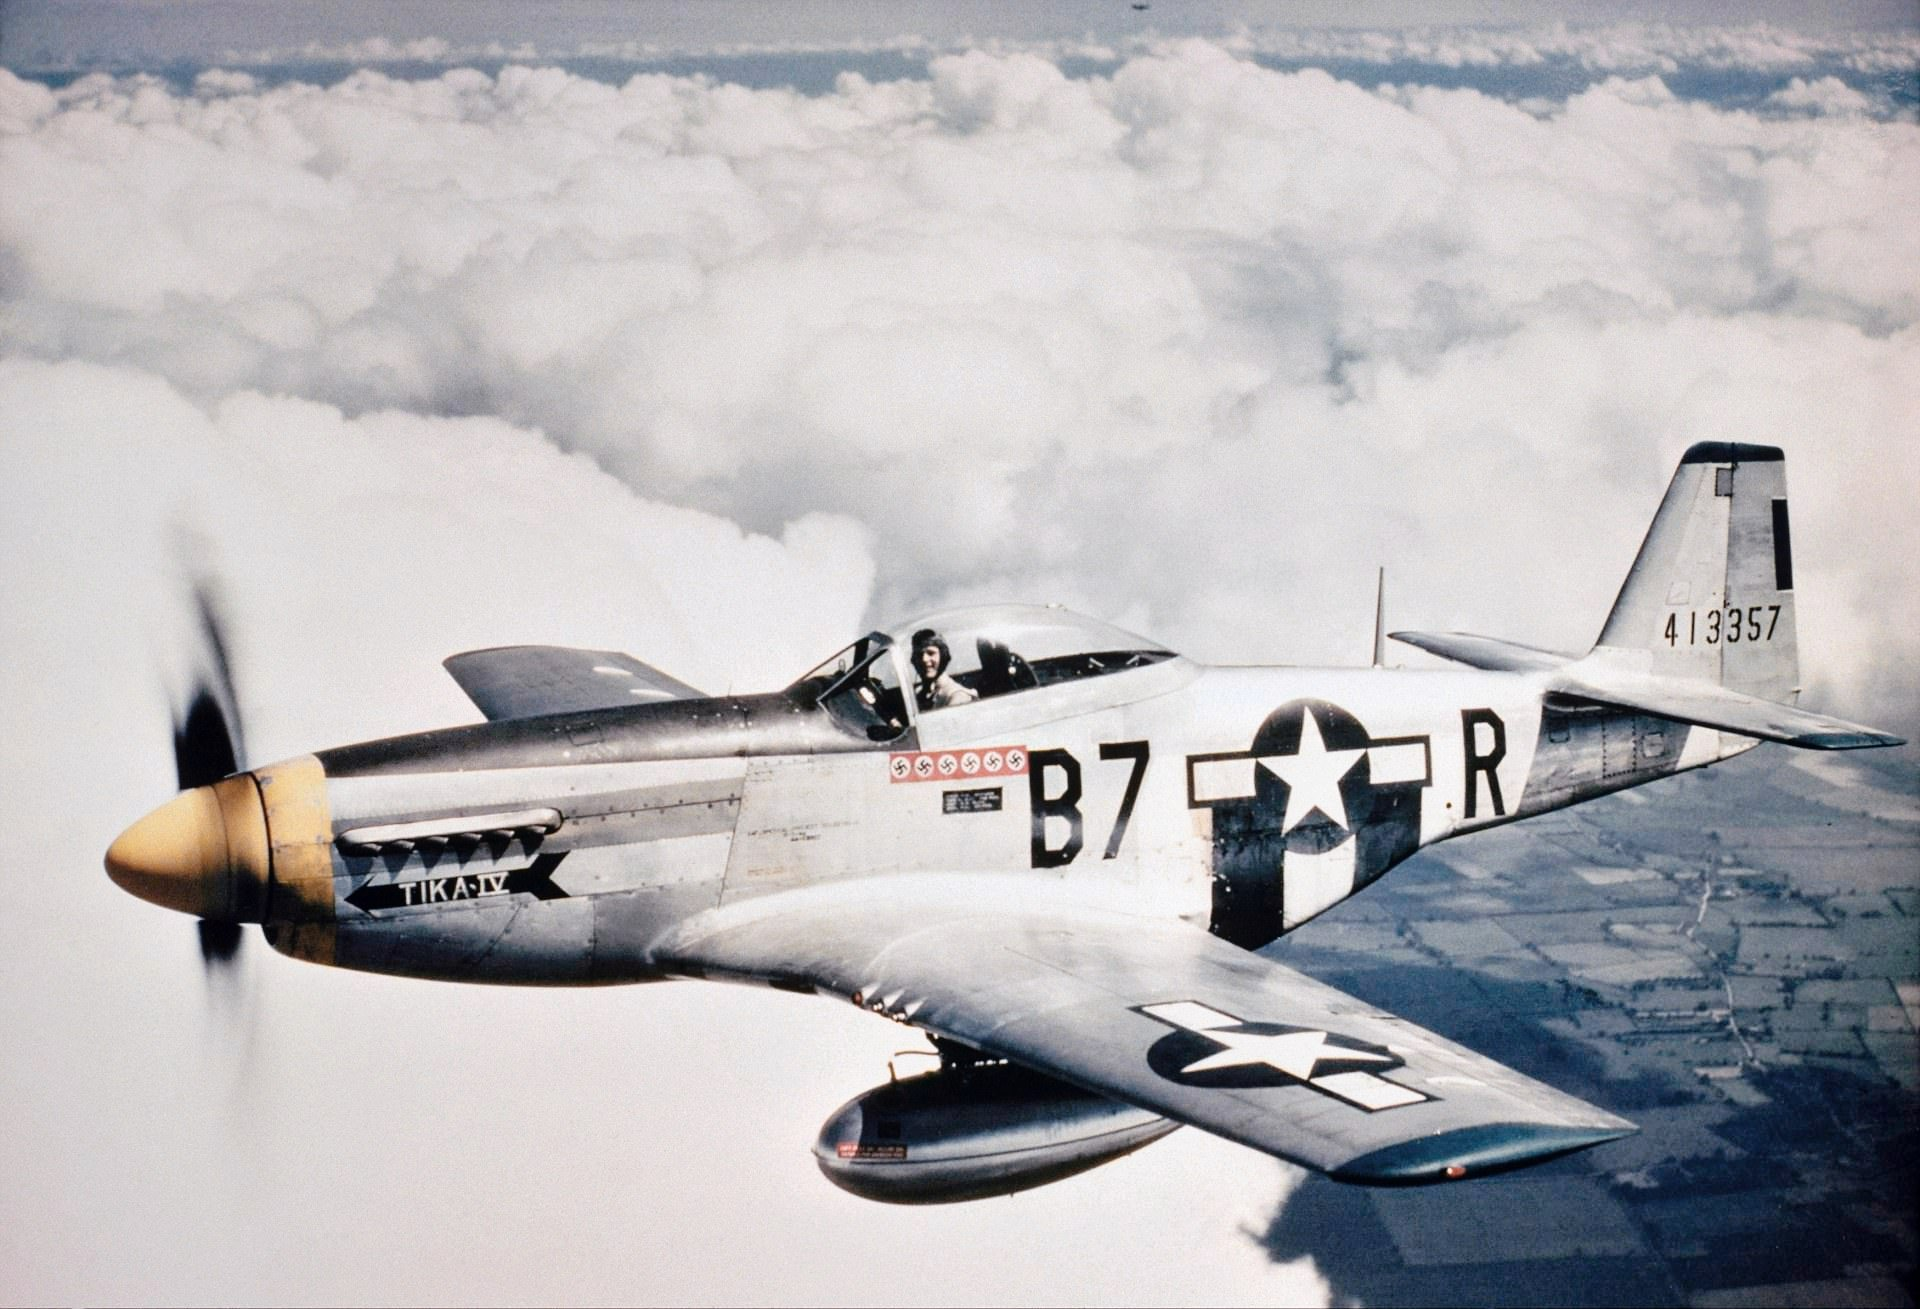
\includegraphics[width=0.90\textwidth]{P-51-mustang}
	\vspace{10pt}
	\caption{North American P-51 Mustang. Image from \cite{wikipedia_mustang}.}
	\label{fig:mustang}
\end{figure}

However it appears that the aeroelasticity problem was not considered from the perspective of natural laminar flow airfoils. This is a surprising fact considering the P-51 Mustang (figure~\ref{fig:mustang}), a fighter aircraft in the Royal Air Force designed in 1940, incorporated a wing with a natural laminar flow airfoil section \citep{green08}. The first aeroelastic study on laminar wings was performed as late as 2011 by \cite{mai11}. This, along with a subsequent investigation by \cite{hebler13}, brought to light a peculiar characteristic of unsteady laminar wings, \textit{i.e.} the presence of non-linearities in the unsteady aerodynamic forces. The classical unsteady aerodynamic theories did not predict non-linear unsteady responses and thus fail to account for such behavior. Inspired by this, \cite{lokattthesis} performed experiments on unsteady NLF airfoils and also found strong non-linearities in the aerodynamic forces. Consistent in the explanation for the non-linearities in all these studies was the role of transition over the wing surface. When transition on the airfoil suction-side was fixed (with a trip) near the leading edge, the non-linearities seemed to disappear. These results indicated a need for a more in-depth study of the evolving boundary layer in such unsteady laminar airfoils. Classical theories negate the role of the boundary layer by invoking the inviscid assumption and it is apparent that such an assumption is no longer be justified for laminar wings. Characteristics of the unsteady boundary layer are the subject of investigation in the present work.

\thesisstructure The thesis is structured as follows:
\begin{itemize}
	\item An overview of the numerical method used for the simulations is given in Chapter 2.
	\item Chapter 3 gives an overview of the numerical simulations performed in the study.
	\item The main conclusions of the current work are given in Chapter 4 along with an outlook for future work.
	\item The next part of the thesis includes the individual papers and internal reports. 
\end{itemize}

%===============================================================================
\chapter{Numerical Method}
%===============================================================================

\section{Numerical Discretization}

The numerical code used for the simulations is Nek5000, which is an open source research code developed by \cite{nek5000} at Argonne National Laboratory. The code solves the incompressible Navier--Stokes equations (\ref{eqn:navier_stokes}) in non-dimensional form:
\begin{subequations}
	\label{eqn:navier_stokes}	
	\begin{eqnarray}
	\frac{\partial u_{i}}{\partial t} + u_{j}\frac{\partial u_{i}}{\partial x_{j}} =  - \frac{1}{\rho}\frac{\partial p}{\partial x_{i}} + \frac{1}{Re}\bigg(\frac{\partial^{2} u_{i}}{\partial x_{j}\partial x_{j}}  \bigg) +f_{i} \\
	\frac{\partial u_{i}}{\partial x_{i}} = 0
	\end{eqnarray}
\end{subequations}
where $x_{i}$ is the coordinate direction, $u_{i}$ is the velocity component, $p$ is the pressure and $Re$ is the defined Reynolds number. The discretization of the Navier--Stokes equations is based on a spectral-element method, first proposed by \cite{patera84}. The method allows the mapping of elements to complex geometries along with a high-order spatial discretization within the elements, thus combining the generality of finite-element methods with the accuracy of spectral methods \citep{patera84}.
The spatial discretization in each element is performed following the $P_{N}$-$P_{N-2}$ \citep{maday89} formulation with velocity represented by high-order Lagrange interpolants through the Gauss--Lobatto--Legendre (GLL) quadrature points, while the pressure is represented on the staggered Gauss-Legendre (GL) quadrature points. The nonlinear terms are treated explicitly by third-order extrapolation (EXT3), while the viscous terms are treated implicitly by a third-order backward differentiation scheme (BDF3). Over-integration is used for the removal of aliasing errors. Nek5000 is written in Fortran 77 and C with efficient scaling for up to 1 million MPI ranks \citep{fischer15}.

%%%%%%%%%%%%%%%%%%%%%%%%%%%%%%%%%%%%%%%%%%%%%%%%%%%%%%%%%%%%%%%%%%%%%%
\section{Relaxation-term large-eddy simulation (RT-LES)}

Owing to the high Reynolds numbers and large time-scales of integration for some of the flow cases, a direct numerical simulation (DNS), which requires a resolution of all the spatial scales of the flow, leads to prohibitively high computational costs. In recent years a technique of wall-resolved large-eddy simulations has emerged as a computationally cheaper alternative to DNS, while also exhibiting the high-fidelity characteristics of DNS.
The technique has been utilized in the studies of spatially developing boundary layers \citep{eitel14}, pipe flows \citep{chin15} and flow over wings \citep{uzun10,lombard15}. The success of the approach has motivated its use in the present work. The wall-resolved LES method used is based on the RT3D variant of the ADM-RT approach first used by \cite{schlatter04}. The method has been shown to be reliable in accurately predicting transition and also preserving the characteristic structures which are seen in the DNS of transitional flows by \cite{schlatter06}. This particular quality of the LES model is crucial since there is a large focus on the unsteady transition in the present work. The LES method supplements the governing equations with a dissipative term $-\chi\mathcal{H}(u)$. The equations of motion for the resolved velocity and pressure thus read as
\begin{subequations}
	\label{eqn:rt_les}	
	\begin{eqnarray}
	\frac{\partial u_{i}}{\partial t} + u_{j}\frac{\partial u_{i}}{\partial x_{j}} =  - \frac{1}{\rho}\frac{\partial p}{\partial x_{i}} + \frac{1}{Re}\bigg(\frac{\partial^{2} u_{i}}{\partial x_{j}\partial x_{j}}  \bigg) + f_{i} -\chi\mathcal{H}(u_{i}), \\
	\frac{\partial u_{i}}{\partial x_{i}} = 0,
	\end{eqnarray}
\end{subequations}	
where $\mathcal{H}$ is a defined high-pass spectral filter and $\chi$ is a model parameter which together with $\mathcal{H}$ determines the strength of the dissipative term. The high-pass filter function $\mathcal{H}$ is defined such that the resultant relaxation-term only has energy in the highest modes, defined by a cut-off mode-number $N_{c}$. Figure~\ref{fig:filter_shape} illustrates the shape of the filter function in spectral space.
\begin{figure}[h]
	\centering
	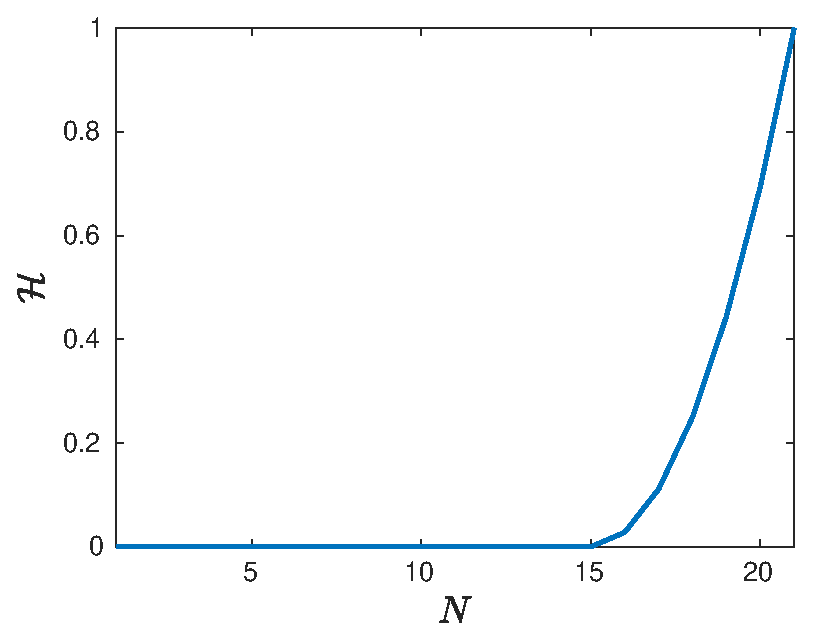
\includegraphics[width=0.60\textwidth]{filter_shape}
	\caption{Transfer function for the spectral coefficients for the filter $\mathcal{H}$ with number of modes $N=21$ and cut-off mode number $N_{c}=16$.}
	\label{fig:filter_shape}
\end{figure}

Several parameter optimization studies were performed to determine the optimum value of $\chi$ and filter shape $\mathcal{H}$ using turbulent channel flow simulations. The LES results were compared with the DNS database of \cite{moser99} and the optimum parameters were further validated for a flow around a wing section at $Re_{c}=400,000$. A good agreement was found between the LES and the DNS data of \cite{hosseini16}, and the optimized parameters were then used for all subsequent simulations.

\section{Arbitrary-Lagrangian-Eulerian (ALE)}

Typical solutions of unsteady fluid flows utilize the Eulerian framework where the coordinate system is fixed in space. A fixed coordinate system however becomes infeasible when the domain boundaries are in motion, as is the case of fluid-structure interaction problems, or when there is a free surface which may lead to a deforming interface. An appropriate method is needed to account or the motion of the boundaries and/or the interior grid points. One such method which substantially simplifies the difficulties arising out of moving boundaries is the Arbitrary-Lagrangian-Eulerian (ALE) method. The method was proposed in a finite-difference framework by \cite{hirt74} and later brought to the spectral-element framework by \cite{ho90,ho91}. The technique combines both the Lagrangian and Eulerian formulations such that, the Navier--Stokes may be solved with the grid points moving with the fluid elements \textit{i.e.} in a Lagrangian framework, or with fixed grid points (Eulerian), or with grid points moving in an arbitrary prescribed manner. The heart of the technique lies in the formulation of the total time rate of change of a quantity in the ALE frame, defined analogously to the material derivative. Thus for a quantity $\mathbf{F(x_{i},t)}$, the change due to small increments $dx_{i}$ and $dt$ may be expressed as \citep{kundu02}
\begin{align}
	dF = \frac{\partial F}{\partial t}dt + \frac{\partial F}{\partial x_{i}}dx_{i}.
	\label{eqn:material_deriv_df}
\end{align}
One may choose to follow any arbitrary path along which this quantity is evaluated, in which case the quantities $dx_{i}$ and $dt$ are related by the velocity of the (grid) point along this arbitrary path $w_{i} = dx_{i}/dt$. The relation results in the expression referred to as the ALE derivative \citep{deville02}, here denoted as $\delta F/\delta t$ to differentiate it from the very similar expression for the material derivative (which is evaluated along the fluid particle trajectory)
\begin{align}
\frac{\delta F}{\delta t} = \frac{\partial F}{\partial t} + w_{i}\frac{\partial F}{\partial x_{i}}.
\label{eqn:ale_derivative}
\end{align}
When $w_{i}$ is equal to the fluid velocity $u_{i}$, we recover the familiar Lagrangian expression for the material derivative $DF/Dt$. On the other hand, when $w_{i}=0$, we get the local (Eulerian) rate of change of the quantity $F$. The material derivative and the ALE derivative share a simple relationship defined using a relative velocity of the fluid particle with respect to the grid motion $c_{i} = u_{i} - w_{i}$, which may be used in the definition of material derivative to obtain
%\begin{subequations}
	\begin{align}
%	\frac{DF}{Dt} = \frac{\partial F}{\partial t} + u_{i}\frac{\partial F}{\partial x_{i}} \nonumber\\
%	\frac{DF}{Dt} = \bigg(\frac{\partial F}{\partial t} + w_{i}\frac{\partial F}{\partial x_{i}}\bigg) + c_{i}\frac{\partial F}{\partial x_{i}} \nonumber \\	
	\frac{DF}{Dt} = \frac{\delta F}{\delta t} + c_{i}\frac{\partial F}{\partial x_{i}}.
	\label{eqn:ale_material_derivative}
	\end{align}
%\end{subequations}
Thus the Navier--Stokes in the ALE formulation may be expressed as 
\begin{subequations}
	\label{eqn:ale_navier_stokes}	
	\begin{align}
	\frac{\delta u_{i}}{\delta t} + (u_{j} - w_{j})\frac{\partial u_{i}}{\partial x_{j}} =  - \frac{1}{\rho}\frac{\partial p}{\partial x_{i}} + \frac{1}{Re}\bigg(\frac{\partial^{2} u_{i}}{\partial x_{j}\partial x_{j}}  \bigg) +f_{i}, \\
	\frac{\partial u_{i}}{\partial x_{i}} = 0,
	\end{align}
\end{subequations}
where $w_{j}$ is the velocity of the grid points. The solution of the Navier--Stokes is then a simple matter of evaluating a suitable grid velocity. 

In many cases, such as the flow over an oscillating airfoil, the velocity of the grid points at the boundary (airfoil surface) may be explicitly known. \cite{ho90,ho91} propose to extend this velocity to the interior points of the domain by solving an elliptic problem for the mesh velocity. In the present work we take a simpler approach to prescribing the mesh velocities in the interior domain. Recognizing the simple trigonometric form of a harmonic pitching motion, all mesh points may simply be prescribed a solid body rotation with the instantaneous angular velocity of the airfoil. However a pure solid-body rotation would also displace the domain boundaries. Therefore a damping function is used to smoothly reduce the rotational velocity away from the airfoil boundary such that the mesh motion is zero at the far-field, inlet and outflow boundaries. Thus for an airfoil with an instantaneous rotation rate of $\Omega_{z}(t)$, the mesh velocity is prescribed as:
\begin{align}
	w_{i}(x,y,z,t) = \underbrace{(\Omega_{z}(t) \times \vec{R})}_{\text{Solid body rotation}} \overbrace{f(|\ \vec{r}\ |)}^{Damping}
	\label{eqn:mesh_velocity}
\end{align}
where $\vec{r}$ is the normal distance of a grid point from the airfoil surface, $\vec{R}$ is the distance from the rotational axis and $f(r)$ is a damping function which can be prescribed in many different ways, depending on one's preferences. The damping function needs to have two essential properties, \textit{i.e.} it must be equal to 1 when $|\vec{r}|=0$, which implies the mesh points at the airfoil boundary move with the surface (solid body rotation at the airfoil surface), and it must smoothly decay to zero close to the far-field boundaries, which allows the external boundaries of the computational domain to remain fixed in physical space. Figure~\ref{fig:mesh_rotation_damping} shows the damping function used in the present work as a function of the normal distance from the airfoil surface.
\begin{figure}[h]
	\centering
	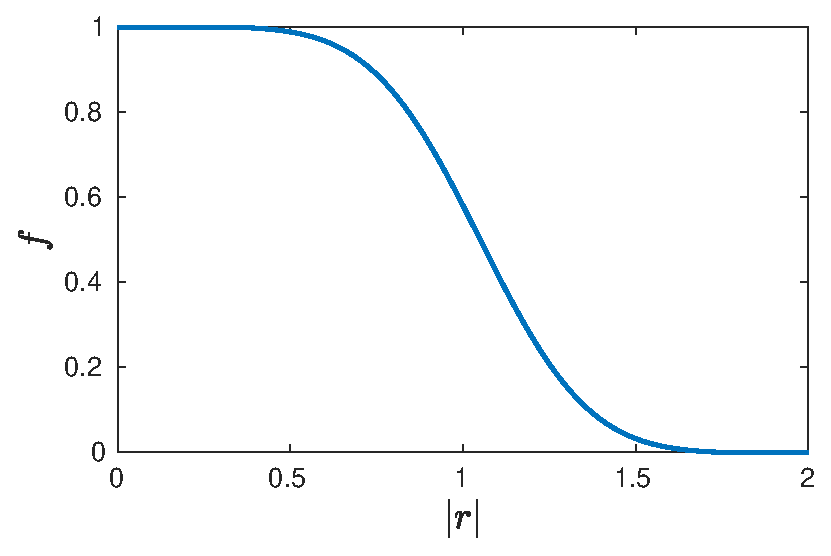
\includegraphics[width=0.55\textwidth]{damping_func}
	\vspace{5pt}
	\caption{Damping function $f(r)$ for the mesh velocities.}
	\label{fig:mesh_rotation_damping}
\end{figure}
The damping function moves the grid points close to the airfoil surface with the same rotational velocity of the airfoil and spreads out the mesh deformation into the interior of the domain. This damping function is calculated once at the beginning of the simulation. Hence all quantities $\Omega_{z}(t),\ \vec{r},\ f(r)$ which are needed for prescribing the mesh velocity are explicitly known at each time-step without the need for solving an elliptic equation as in \cite{ho90,ho91}. 

\section{Free-stream turbulence}

Isotropic, homogeneous free-stream turbulence is prescribed at the inlet and far-field boundaries to add small disturbances to the flow-field, which simulate the disturbances found in a wind-tunnel or in free-flight conditions. The free-stream turbulence is prescribed as a superposition of Fourier modes with a random phase shift. The maximum and minimum amplitudes of the wavenumber vector are prescribed quantities and are limited by the resolution of the spatial discretization and size of the domain respectively. The wavenumber space between the minimum and the maximum is divided into 20 concentric shells with each shell representing the amplitude of the three-dimensional wavenumber vectors lying on the shell. 20 points are randomly chosen on each shell with the location of each point representing the three-dimensional components of the wavenumber vector. Thus the free-stream turbulence is represented by a total of 400 fourier modes. Care is taken to avoid very small wavenumber components which result in wavelengths in physical space that are larger than the computational domain. The streamwise length scales are transformed to a temporal frequency by invoking Taylor's frozen turbulence hypothesis and using the local mean streamwise velocity at the inlet for the space-time conversion. The amplitude of the free-stream modes on each spherical shell is scaled using the von K\'arm\'an spectrum. Figure~\ref{fig:fst_duct} shows an instantaneous visualization of the streamwise velocities in a doubly-periodic duct flow case with high ($5\%$) free-stream turbulence intensity prescribed at the the inlet. Figure~\ref{fig:ti_decay} shows the spatial decay of turbulence intensity. After a small initial distance of adjustment from the inlet, the turbulence intensity decays as a power law. A very similar method for generating free-stream turbulence for simulations of flat-plate boundary layers is used by \cite{schlatterdiploma,brandt04,schlatter08} and more recently for wind turbine simulations by \cite{kleusberglicenciate}.

\begin{figure}[h]
	\centering
	\begin{subfigure}[t]{0.49\textwidth}
		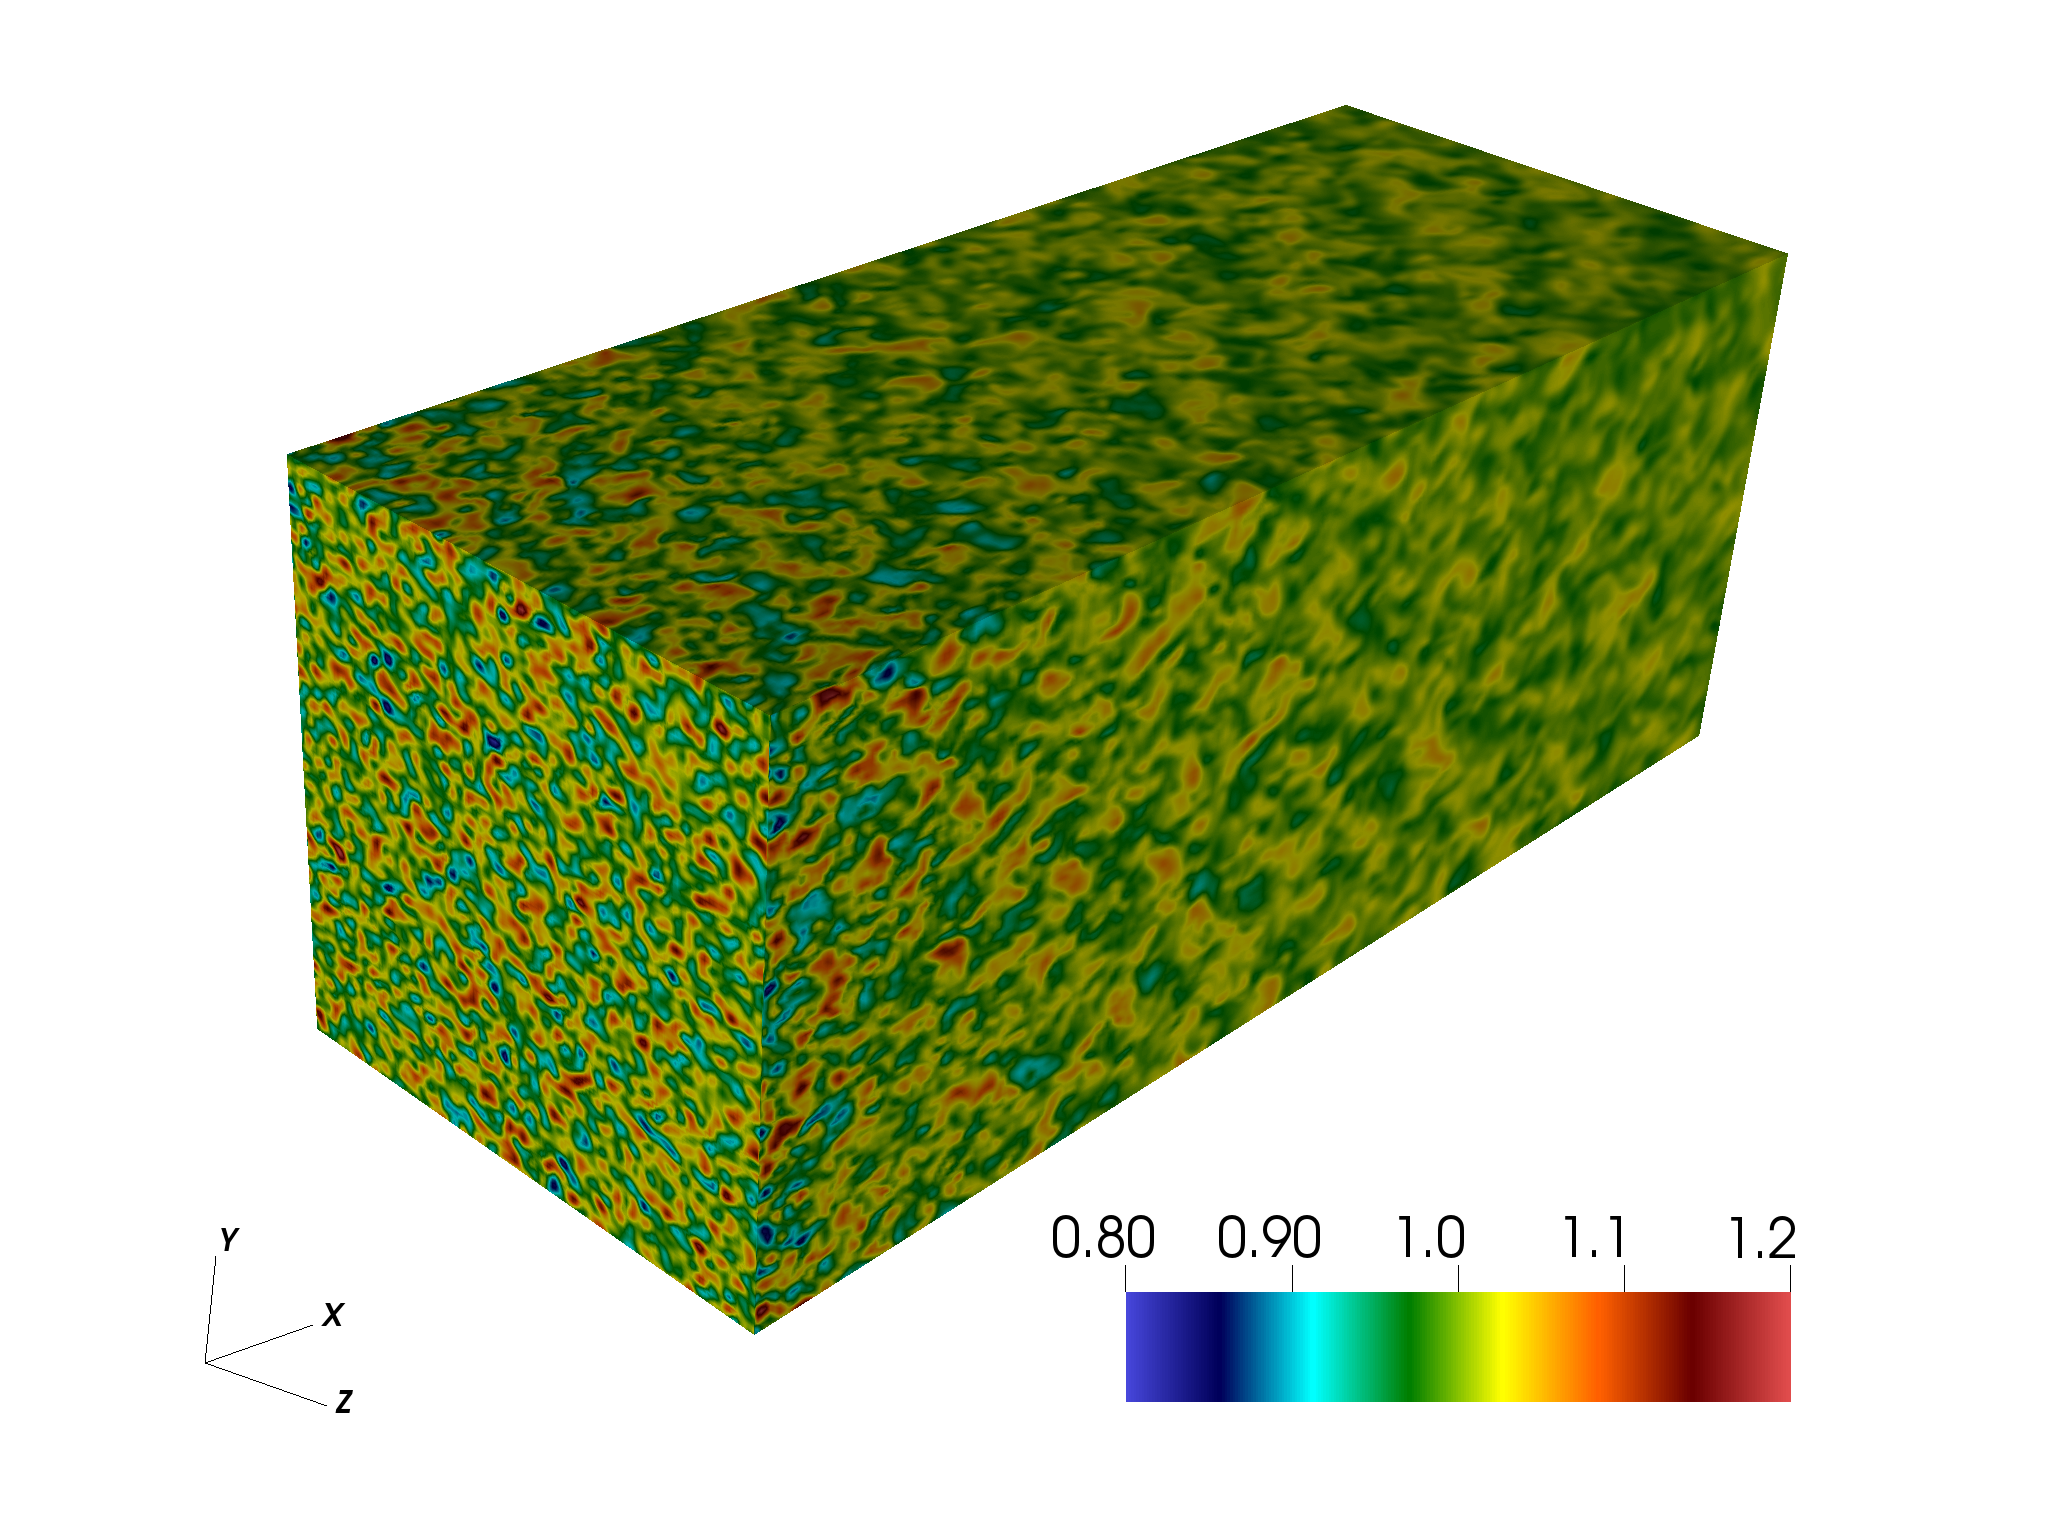
\includegraphics[width=1\textwidth]{fst_duct_vx0000.png}
		\caption{Visualization of free-stream turbulence prescribed at the inlet for a doubly periodic duct flow. Colors represent the instantaneous streamwise velocity.}
		\label{fig:fst_duct}
	\end{subfigure}
	\begin{subfigure}[t]{0.49\textwidth}
		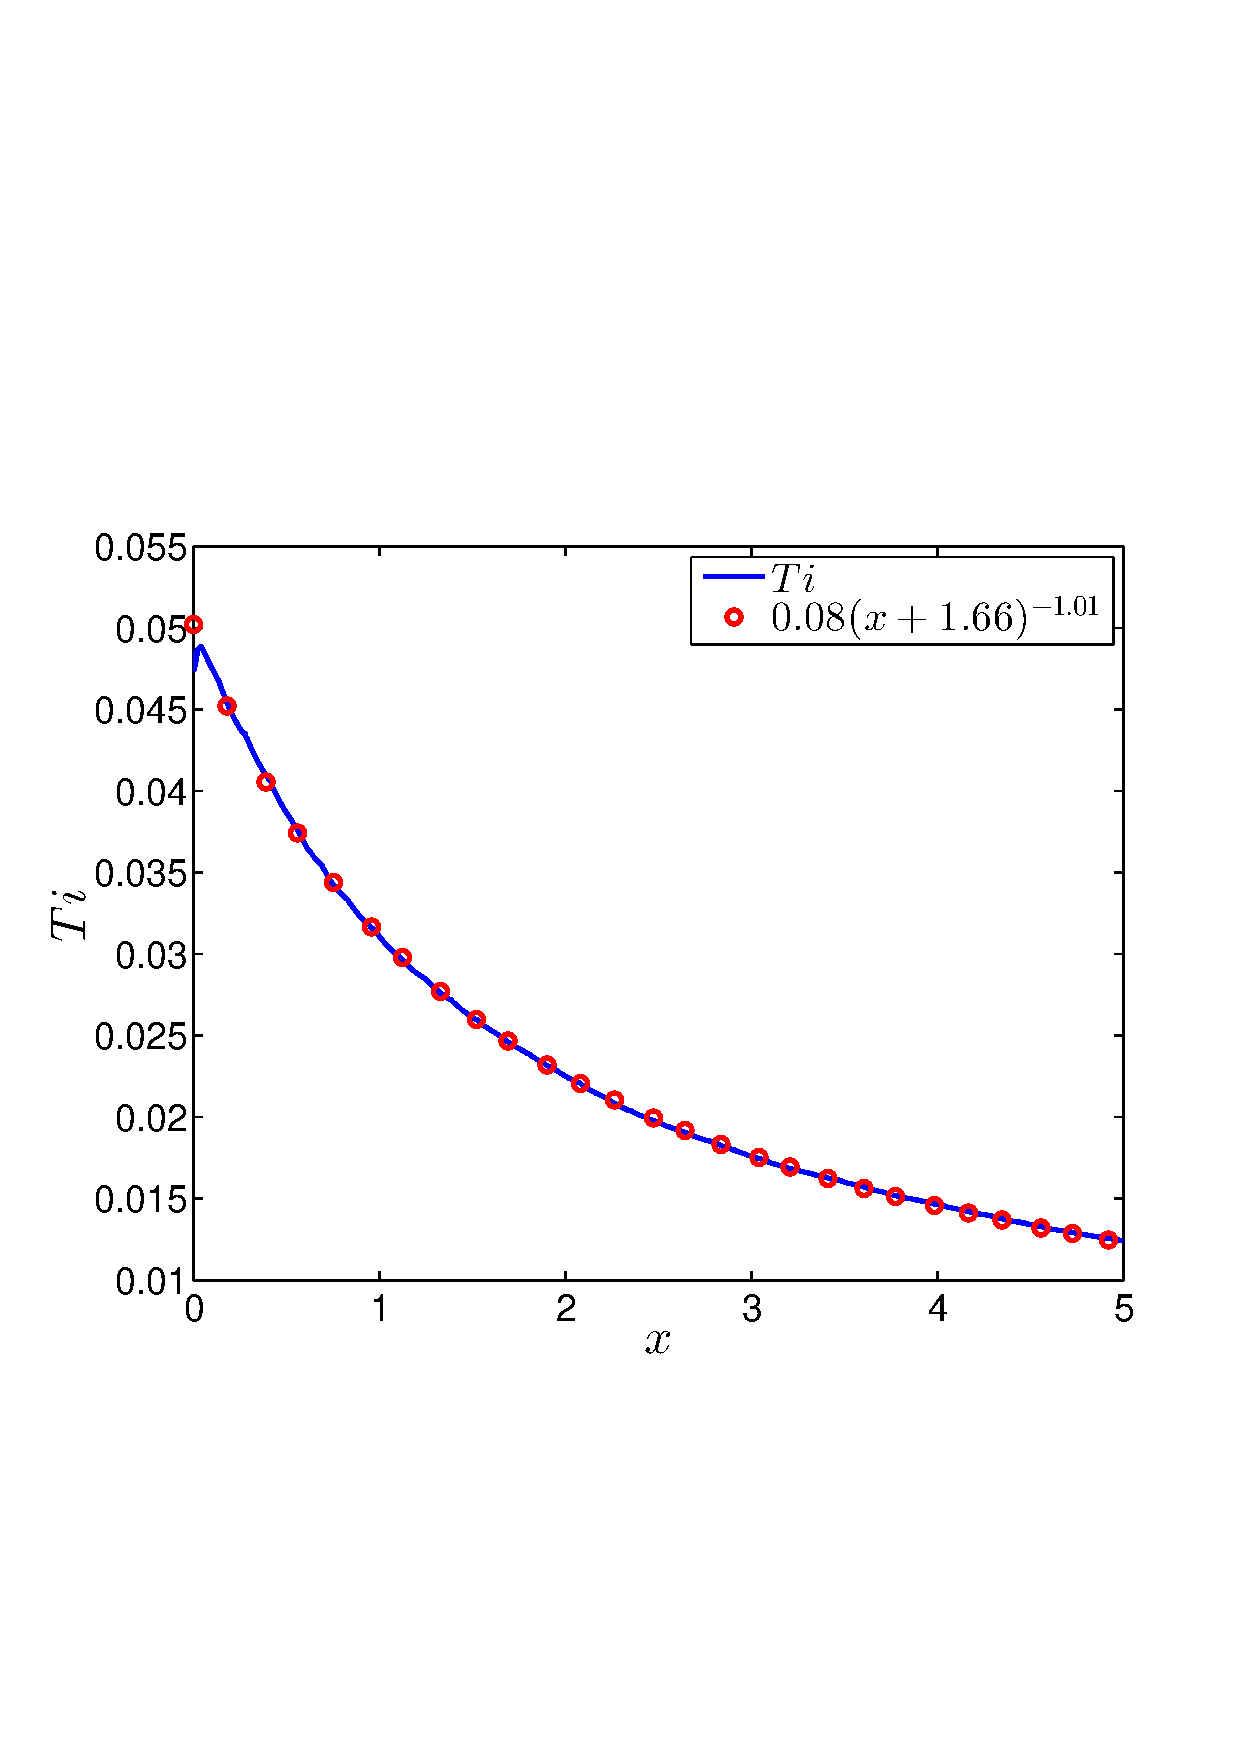
\includegraphics[width=1\textwidth]{ti_decay}
		\caption{Decay of turbulence intensity with streamwise distance, along with the least-squares fit of a power law.}
		\label{fig:ti_decay}
	\end{subfigure}
\end{figure}

%===============================================================================
\chapter{Overview of numerical simulations}
%===============================================================================

\section{Flow around unsteady wings}

The unsteady experiments of \cite{mai11,hebler13} and \cite{lokattthesis} have shown that aerodynamic non-linearities are related to the movement of transition over the suction side of the airfoil. Thus unsteady boundary layer dynamics play an important role in aerodynamic response of NLF airfoils. The present work investigates the unsteady boundary layers with a particular focus on unsteady transition with the aim to shed light on the phenomenon of non-linear unsteady aerodynamic response. The airfoil used in the investigation is the ED36F128 (with a $13.8^{\circ}$ flap deflection), designed at the Aeronautical and Vehicle Engineering department at KTH. It is a natural laminar flow airfoil, which has been used in several steady and unsteady experiments \citep{lokatt17,lokattthesis}. The unsteady experiments have shown the non-linearities that appear to be typical of laminar airfoils \citep{lokattthesis}. The results of the steady and unsteady experiments using this airfoil have been made available to us by Dr. Eller and Dr. Lokatt. Non-linearities in the unsteady aerodynamic forces are observed for only a certain range of angle of attack $\alpha$. Therefore a careful assessment of the data was needed in order to select the right parameter range where the relevant flow physics could be observed in the numerical simulations. The data in the experimental campaign was gathered primarily through pressure taps located around airfoil for the calculation of unsteady aerodynamic forces. Thus measurements of the unsteady boundary layer characteristics was not available through the experimental data. Calculations using an integral boundary layer code XFOIL \citep{drela89}, were used to complement the experimental data and better evaluate the state of the boundary layer in the static measurements.

Figure~\ref{fig:tr_xfoil_100_750} shows the calculated transition locations for two different Reynolds numbers ($Re_{c}=100,000$ and $Re_{c}=750,000$) using XFOIL and figure~\ref{fig:765k_static_cz_foil} shows the experimentally measured normal force coefficient as well as calculations from XFOIL for $Re_{c}=750,000$. For the higher Reynolds number case, transition location varies sharply with angle of attack within the range $3.4^{\circ}<\alpha<6.5^{\circ}$. Aerodynamic non-linearities can also be observed approximately within the same angle of attack range (figure~\ref{fig:765k_static_cz_foil}). For the lower Reynolds number case, no experimental data is available. Therefore solely XFOIL calculations are used and the parameter range is selected where the transition location varies rapidly with angle of attack. This is found for an angle of attack range of $6.7^{\circ}<\alpha<8.0^{\circ}$.
\begin{figure}[!h]
	\centering
	\begin{subfigure}[t]{0.45\textwidth}
		\caption{}
		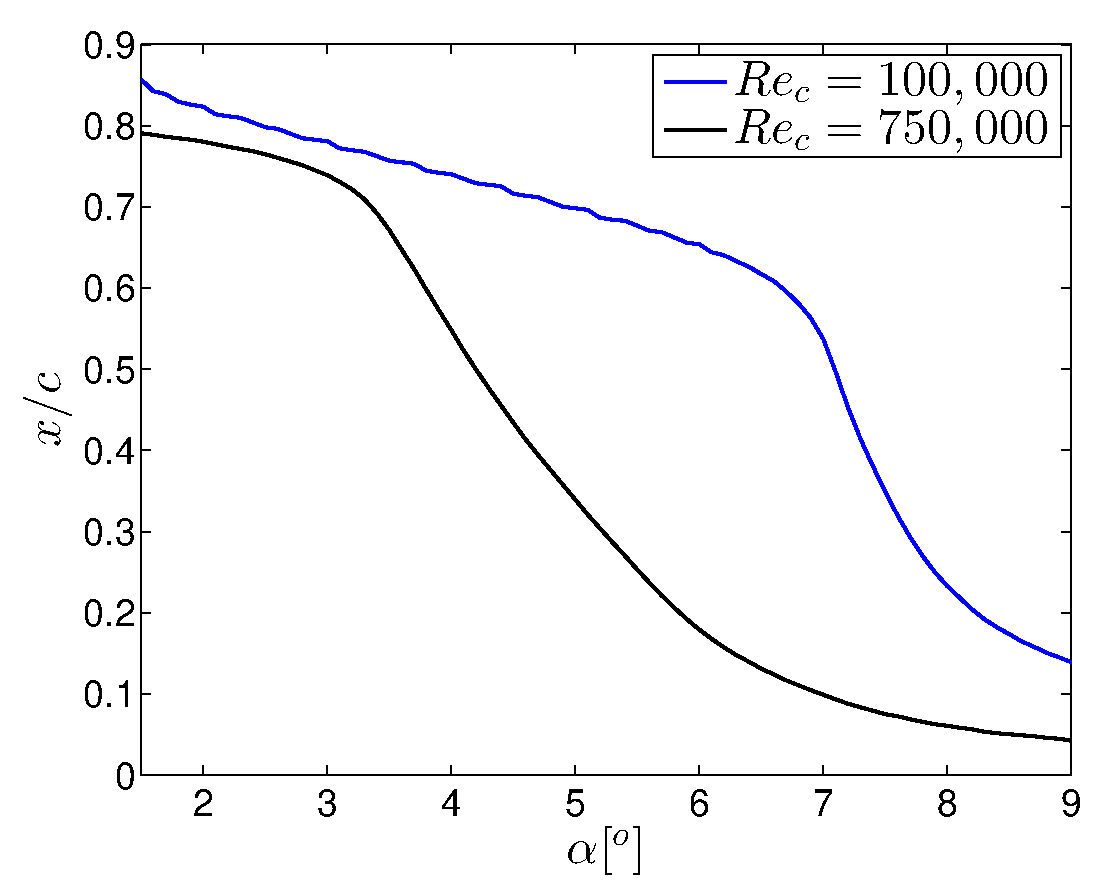
\includegraphics[width=1\textwidth]{tr_xfoil_100_750}
		\label{fig:tr_xfoil_100_750}		
	\end{subfigure}
	\begin{subfigure}[t]{0.45\textwidth}
		\caption{}
		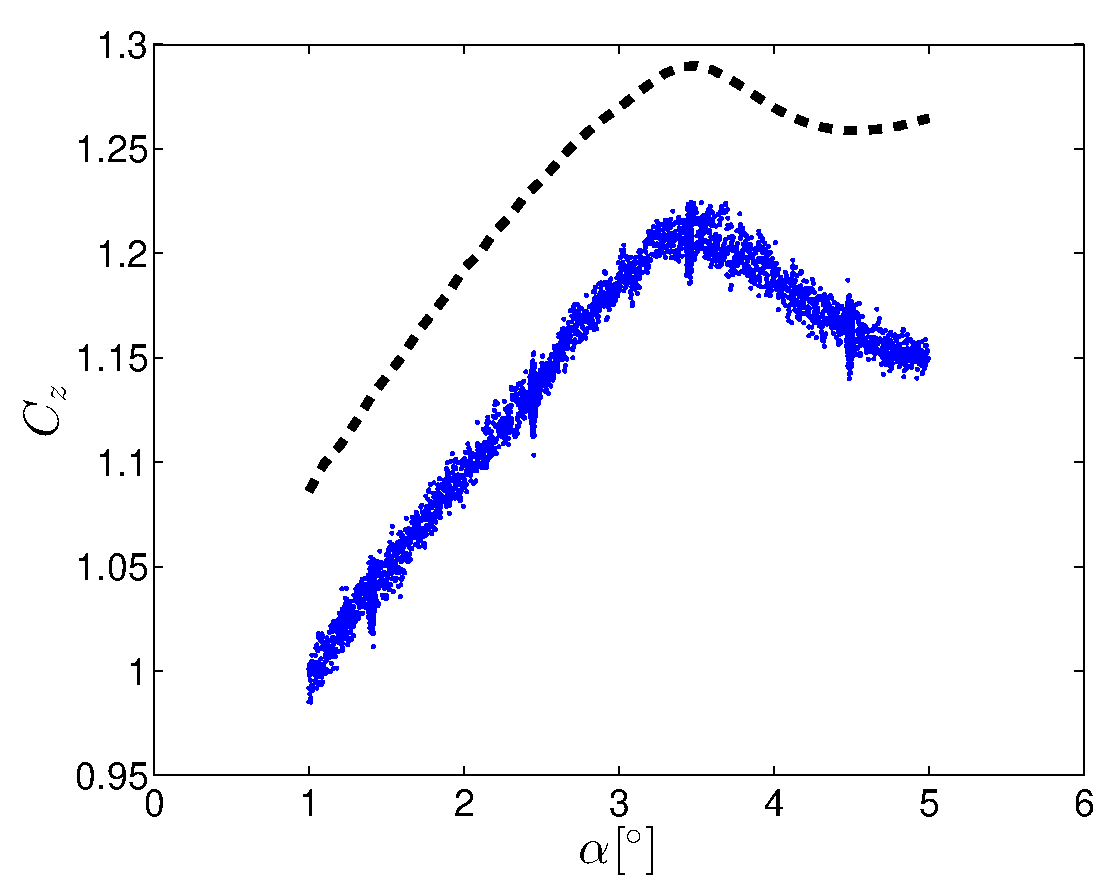
\includegraphics[width=1\textwidth]{765k_static_model_cz_xfoil}
		\label{fig:765k_static_cz_foil}
	\end{subfigure}
	\caption{(a) Transition location calculated using XFOIL for two different Reynolds numbers. (b) Normal force coefficient measured in experiments (dots) and from XFOIL calculations (dashed line) for $Re_{c}=750,000$.}		
\end{figure}
Numerical simulations are performed with stationary airfoils to ensure the expected static boundary layer characteristics are captured by the numerical simulations.  Figure~\ref{fig:overview_la2_750k_stationary} depicts the instantaneous vortical structures in the flow for $Re_{c}=750,000$ for an angle of attack $\alpha=2.4^{\circ}$ and $\alpha=4.4^{\circ}$ which shows the change in boundary layer characteristics in the static cases. Similarly, figure~\ref{fig:overview_isocontour_aoa} shows the static boundary layer characteristics for $Re_{c}=100,000$ at $\alpha=6.7^{\circ}$ and $\alpha=8.0^{\circ}$.
\begin{figure}[h]
	\centering
	\begin{subfigure}[t]{0.49\textwidth}
		\caption{$\alpha=2.4^{\circ}$}		
		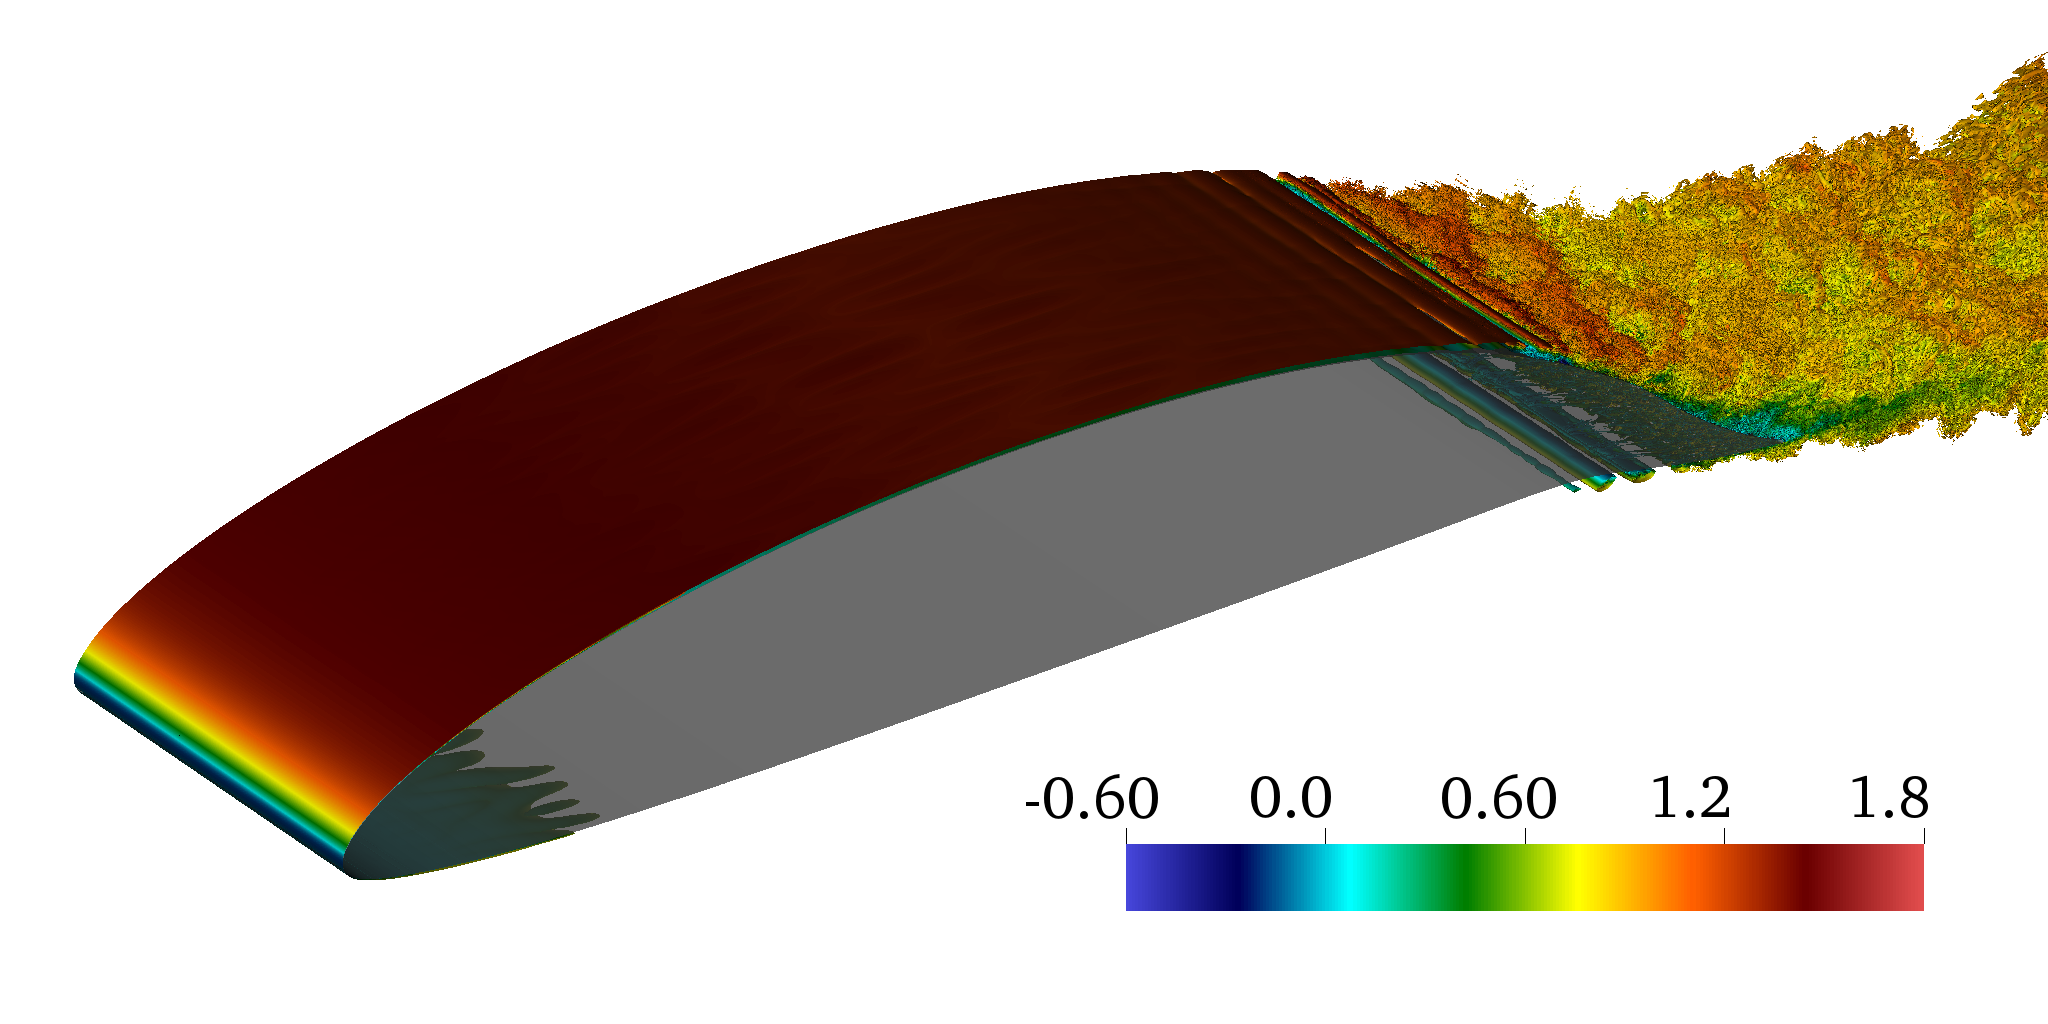
\includegraphics[width=1\textwidth]{paper2/imgs2/pitch_re750k0001}
		\label{fig:overview_la2_aoa24}
	\end{subfigure}
	\begin{subfigure}[t]{0.49\textwidth}
		\caption{$\alpha=4.4^{\circ}$}		
		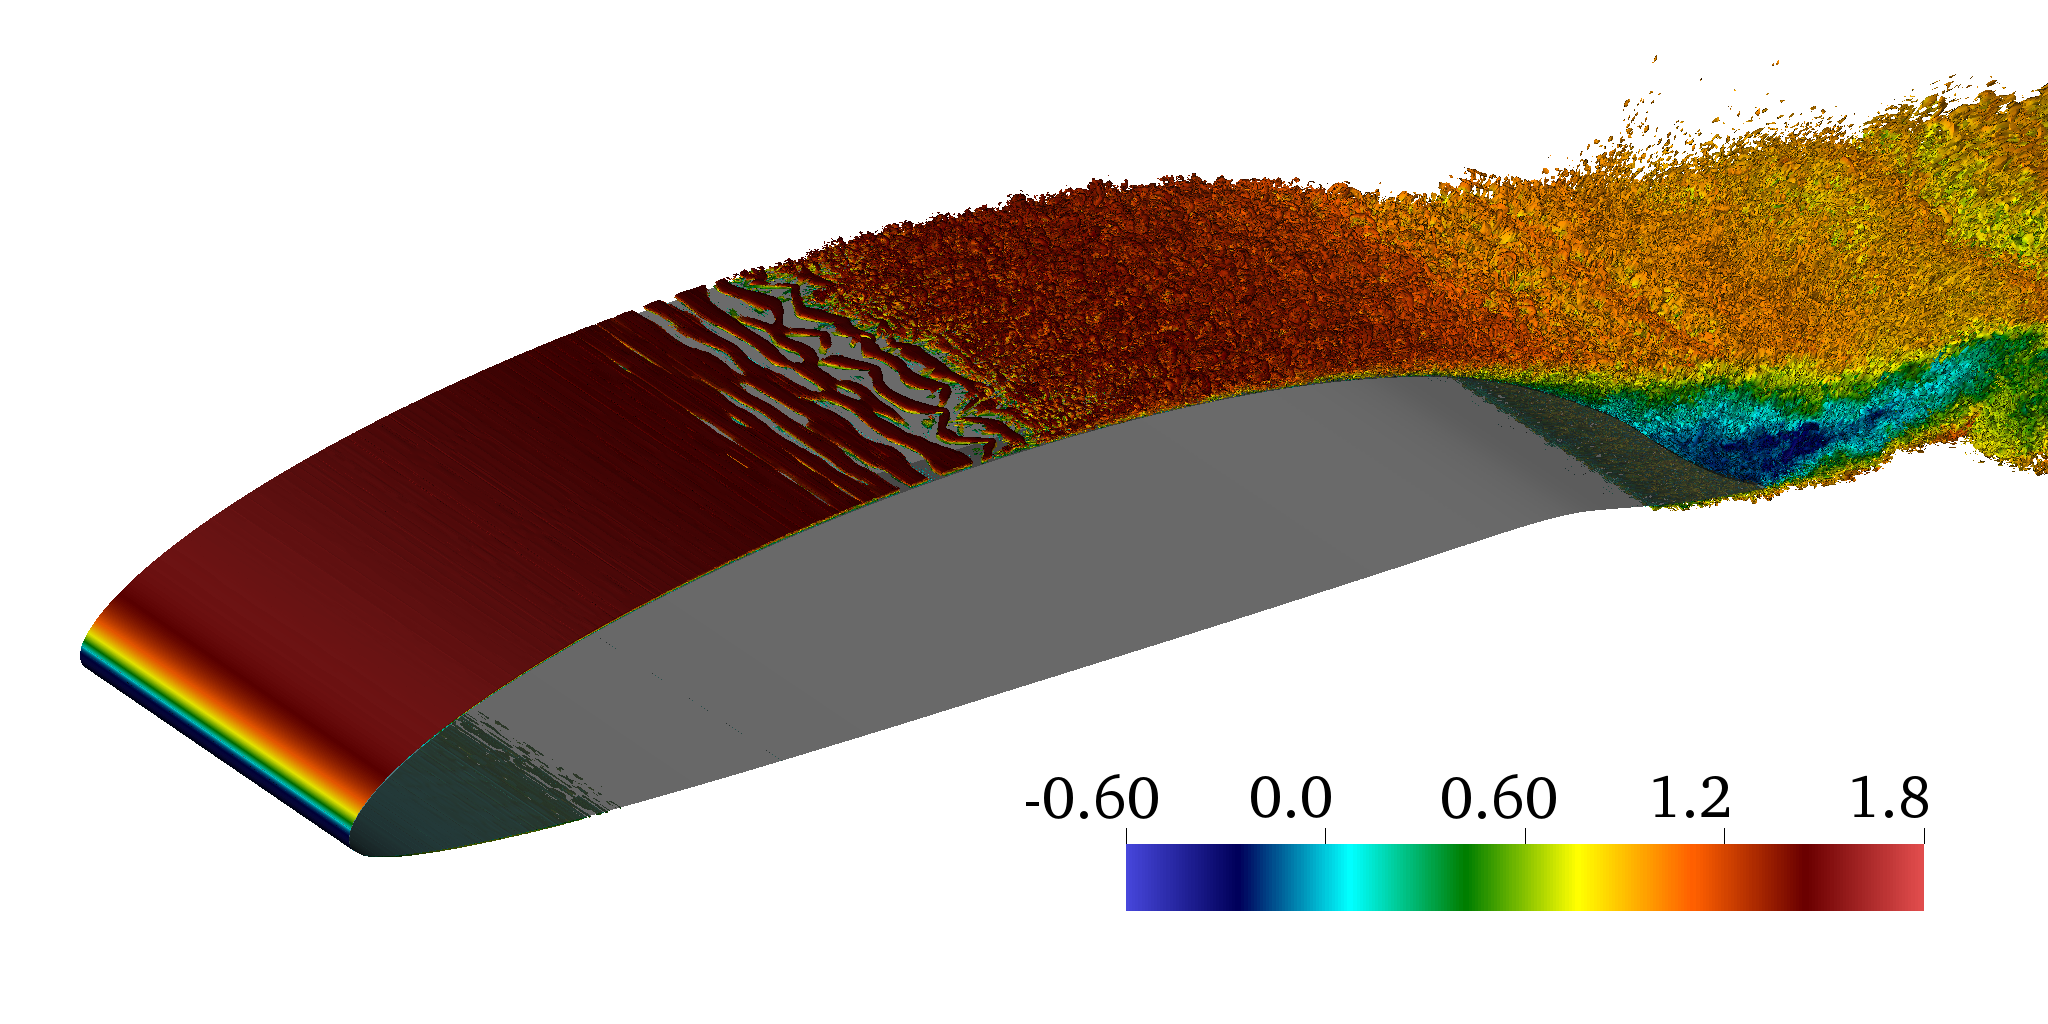
\includegraphics[width=1\textwidth]{paper2/imgs2/pitch_re750k0002}
		\label{fig:overview_la2_aoa44}		
	\end{subfigure}	
	\caption{Instantaneous vortical structures identified by the $\lambda_{2}$ criterion for the two stationary angle of attack simulations at $Re_{c}=750,000$.}
	\label{fig:overview_la2_750k_stationary}
\end{figure}

\begin{figure}[t]
	\begin{subfigure}[b]{0.49\textwidth}
		\centering
		\caption{$\alpha=6.7^{\circ}$}		
		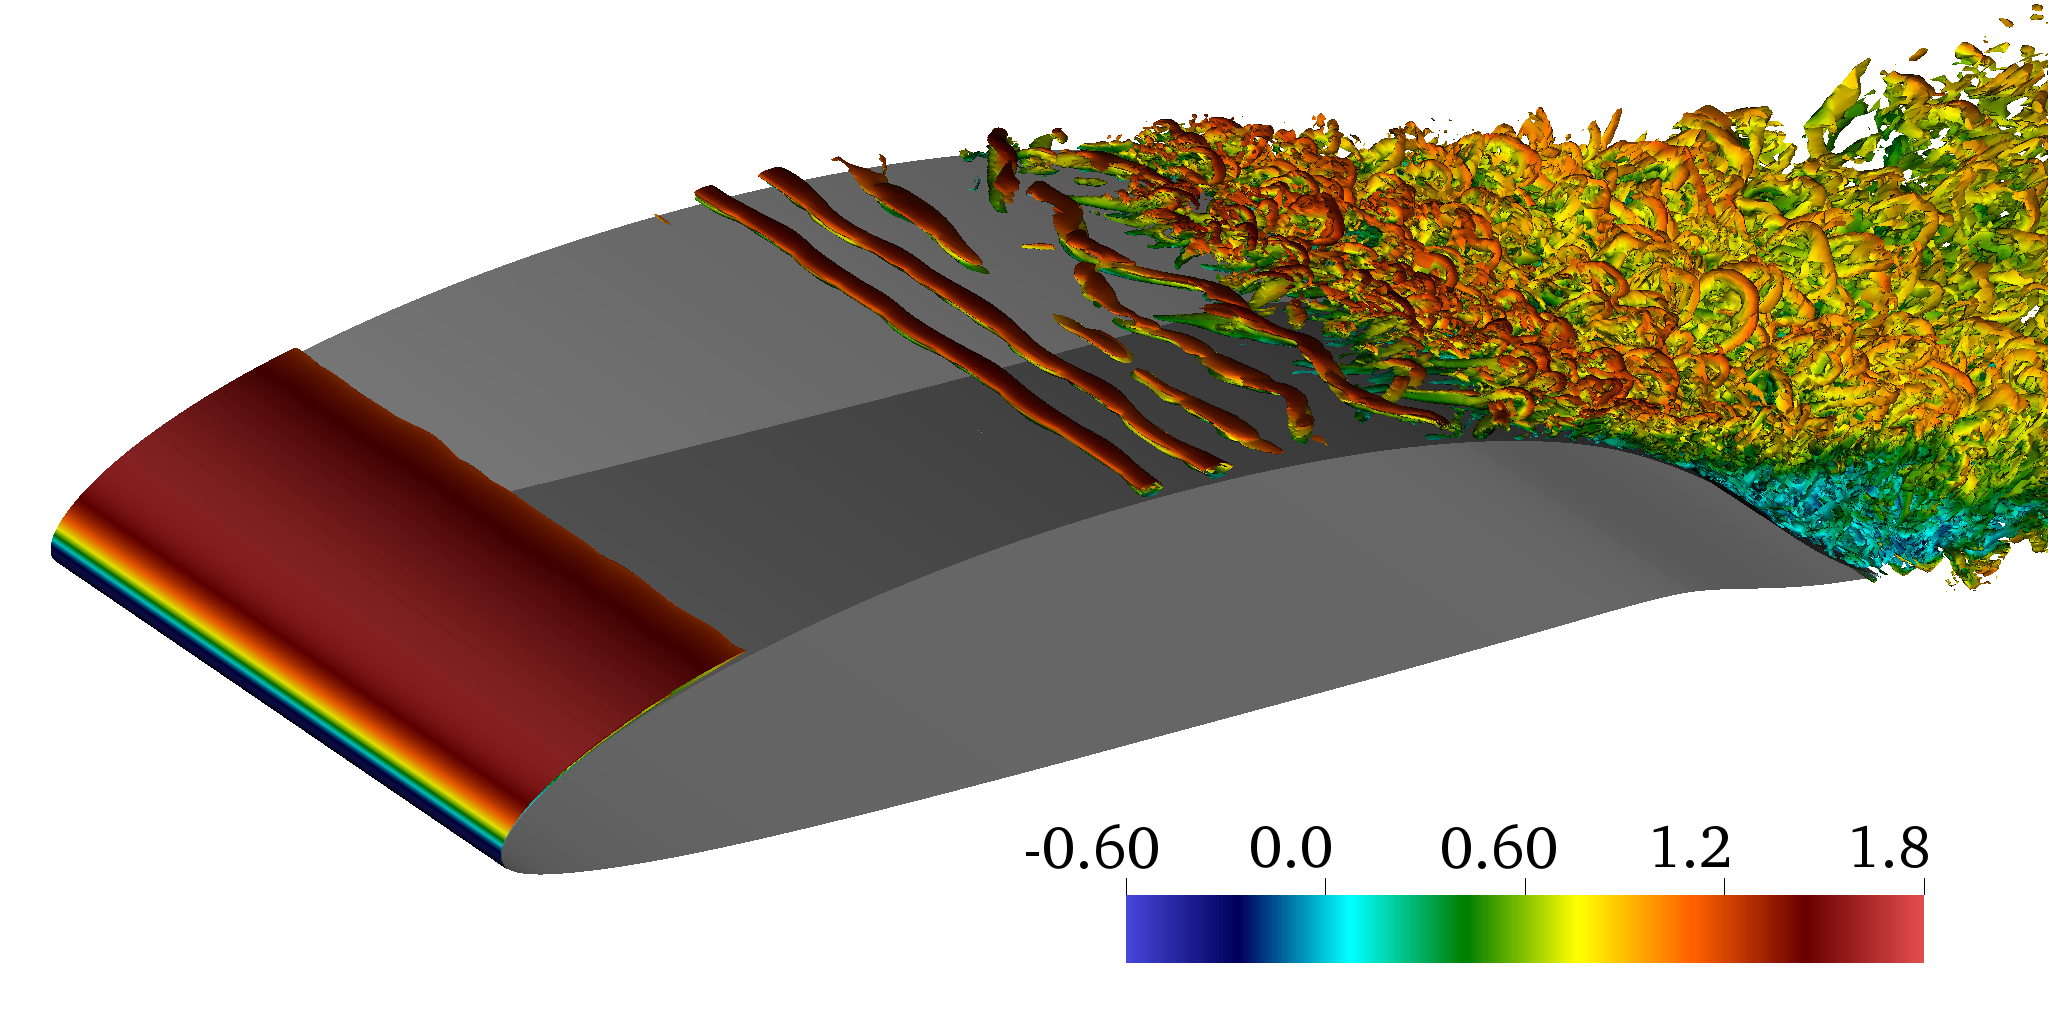
\includegraphics[width=1\textwidth]{paper3/imgs/re100k_static67_0001}
		\label{fig:overview_aoa67_iso}
	\end{subfigure}
	\begin{subfigure}[b]{0.49\textwidth}
		\centering
		\caption{$\alpha=8.0^{\circ}$}		
		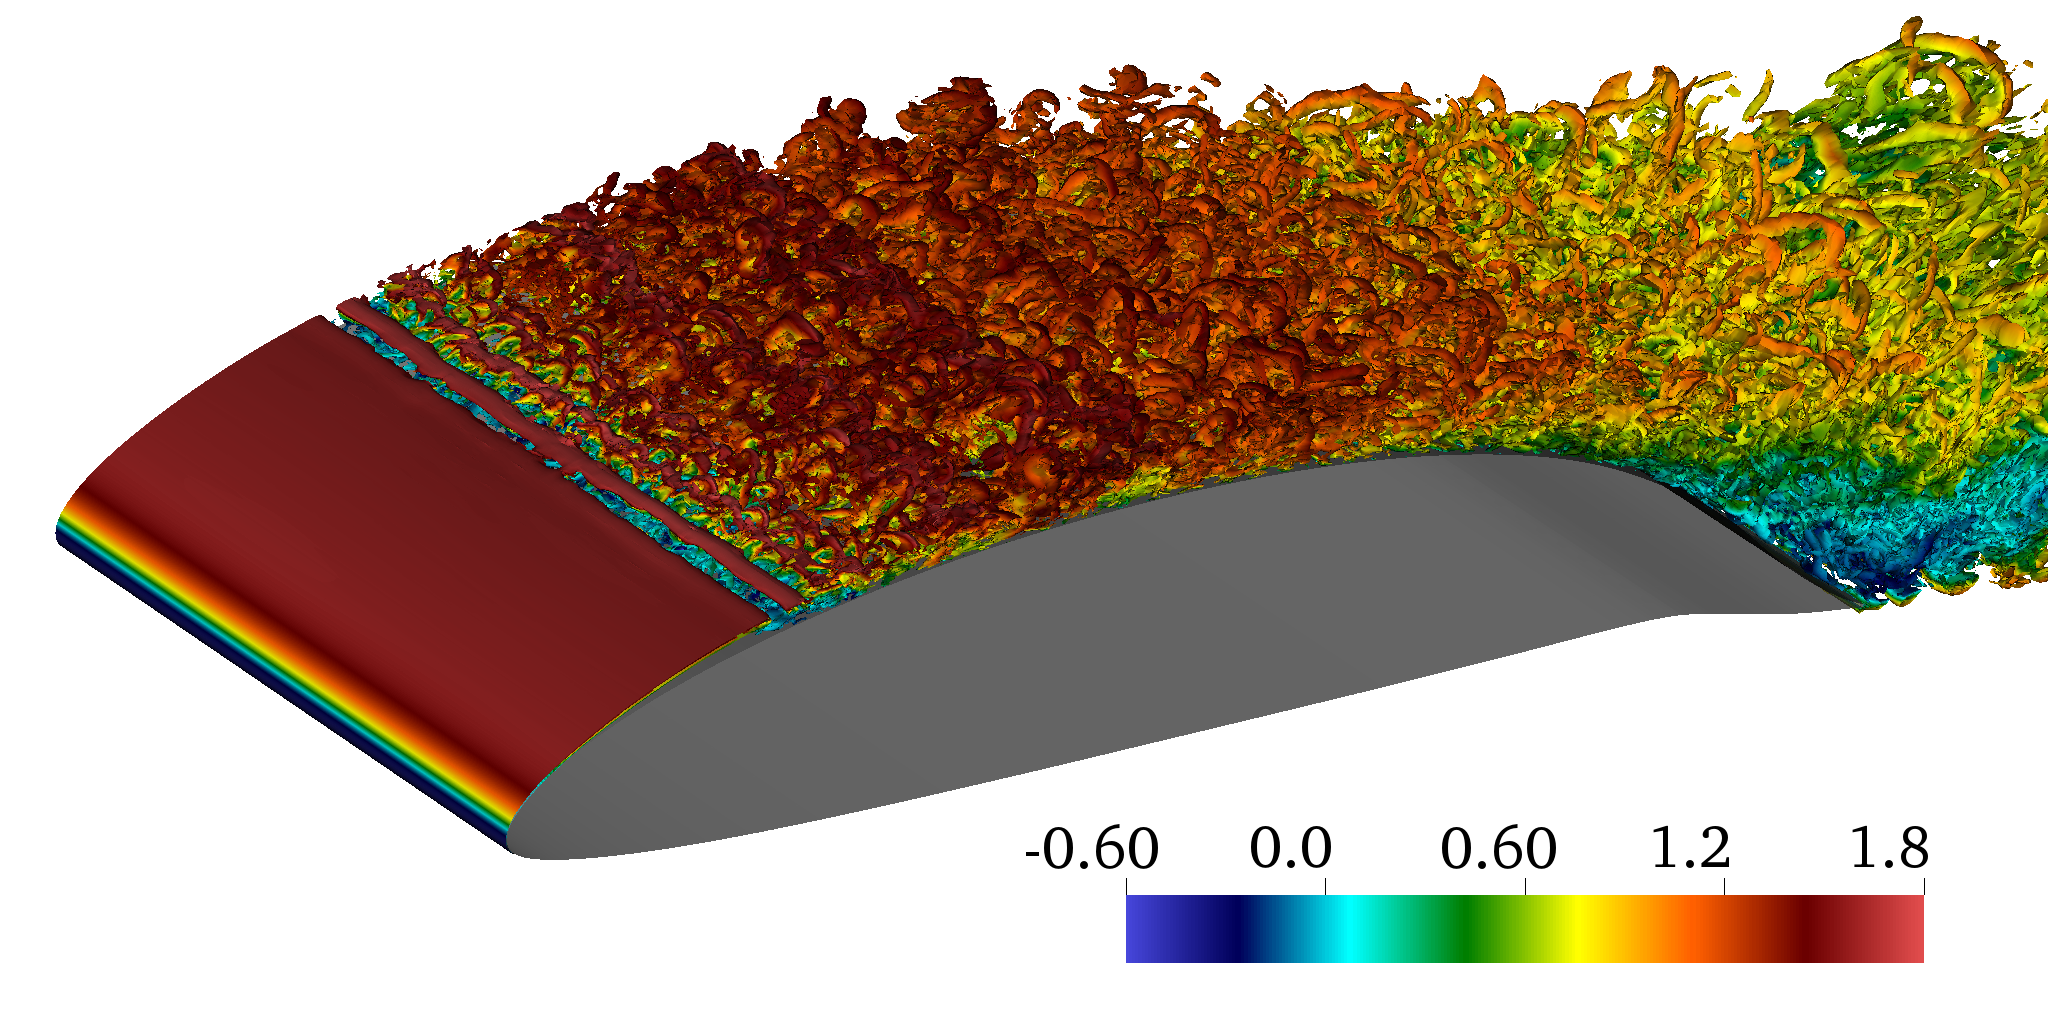
\includegraphics[width=1\textwidth]{paper3/imgs/re100k_static80_0001}
		\label{fig:overview_aoa80_iso}
	\end{subfigure}
	\caption{Isocontours of instantaneous $\lambda_{2}$ structures observed for two different (stationary) angles of attack at $Re_{c}=100,000$.}
	\label{fig:overview_isocontour_aoa}
\end{figure}

For both the Reynolds number cases, significant temporal variation of transition location is also found for the unsteady cases. Figure~\ref{fig:overview_transition_alpha} shows the variation of transition with respect to $\alpha$. The transition locations were calculated using thresholds on the instantaneous spanwise-averaged Reynolds stress $\overline{u'v'}$ and spanwise fluctuation intensity $\overline{w'w'}$. For the lower Reynolds number case the boundary layer also develops a leading-edge laminar separation bubble during the pitch cycle which significantly influences the boundary-layer dynamics.

\begin{figure}[t]
	\begin{subfigure}[b]{0.49\textwidth}
		\centering		
		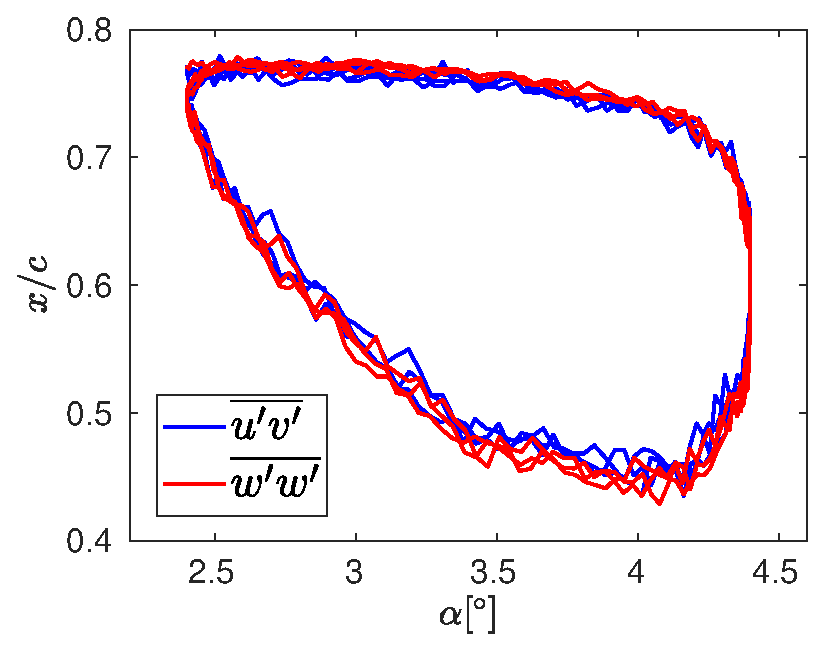
\includegraphics[width=1\textwidth,height=0.80\textwidth]{imgs/750k_transition_alpha.eps}
	\end{subfigure}
	\begin{subfigure}[b]{0.49\textwidth}
		\centering	
		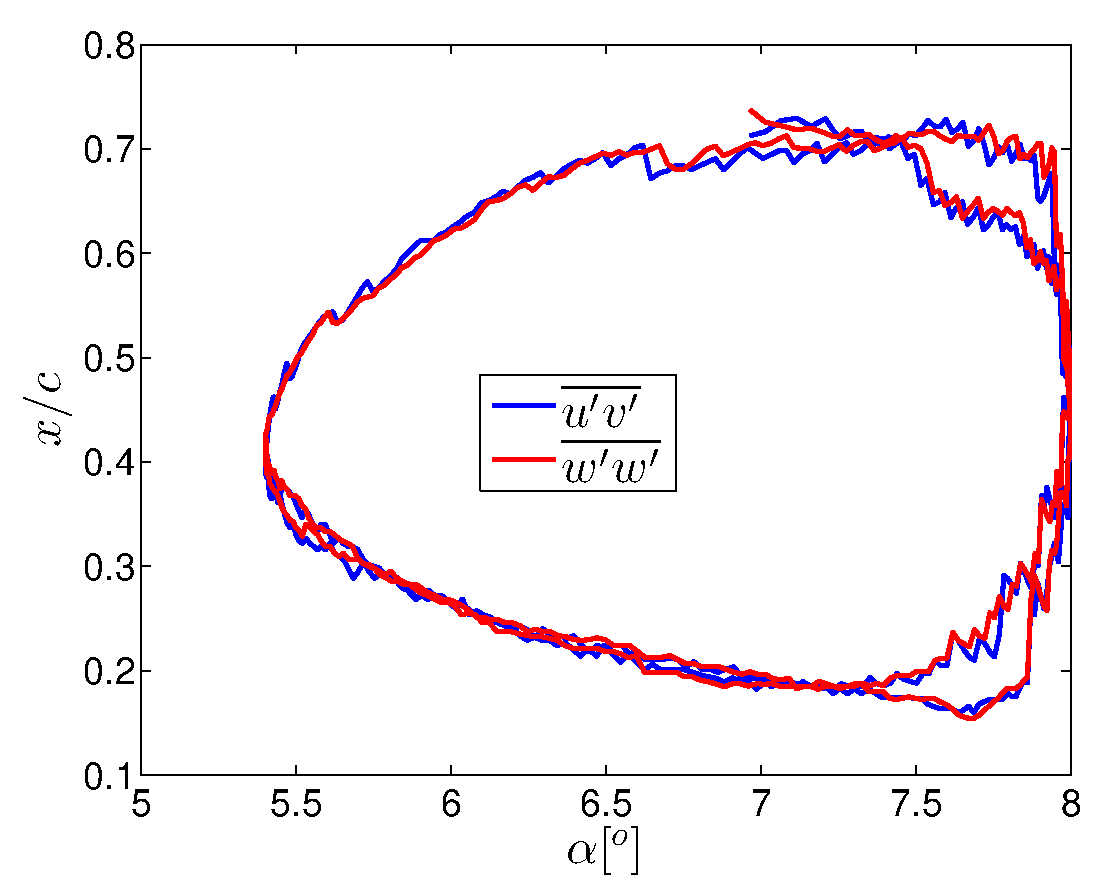
\includegraphics[width=1\textwidth]{paper3/imgs/transition_alpha.eps}
	\end{subfigure}
	\caption{Phase portraits of transition location for (left) $Re_{c}=750,000$ and (right) $Re_{c}=100,000$.}
	\label{fig:overview_transition_alpha}
\end{figure}


\section{Flow around a stationary wing section}

The final paper in the thesis deals with the study of the boundary layer over a wing section at a chord-based Reynolds number of $Re_{c}=1,000,000$. The airfoil used for the study is the asymmetric NACA 4412. A DNS database for the flow around the same airfoil at $Re_{c}=400,000$ is available and comparisons are made between the two cases to assess the effects of changing Reynolds number on the developing boundary layer. The numerical setup is done in a manner very similar to the computational study by \cite{hosseini16}. Figure~\ref{fig:overview_flow_field_re1000k} shows a section of the numerical grid and the instantaneous vortical structures in the flow field. Figure~\ref{fig:overview_beta_Reth_Ret} shows a comparison of the different measures of the boundary layer over the chord-wise distance for the two different Reynolds numbers. While both wall-shear stress (indicated by $Re_{\tau}$) and boundary layer thickness (measured with momentum thickness Reynolds number $Re_{\theta}$) change between the two cases, the Clauser parameter stays nearly the same throughout the chord. This allows comparisons across different Renolds numbers without ambiguity since the pressure gradient histories remain the same with changing Reynolds numbers. 
\begin{figure}[t]
	\centering
	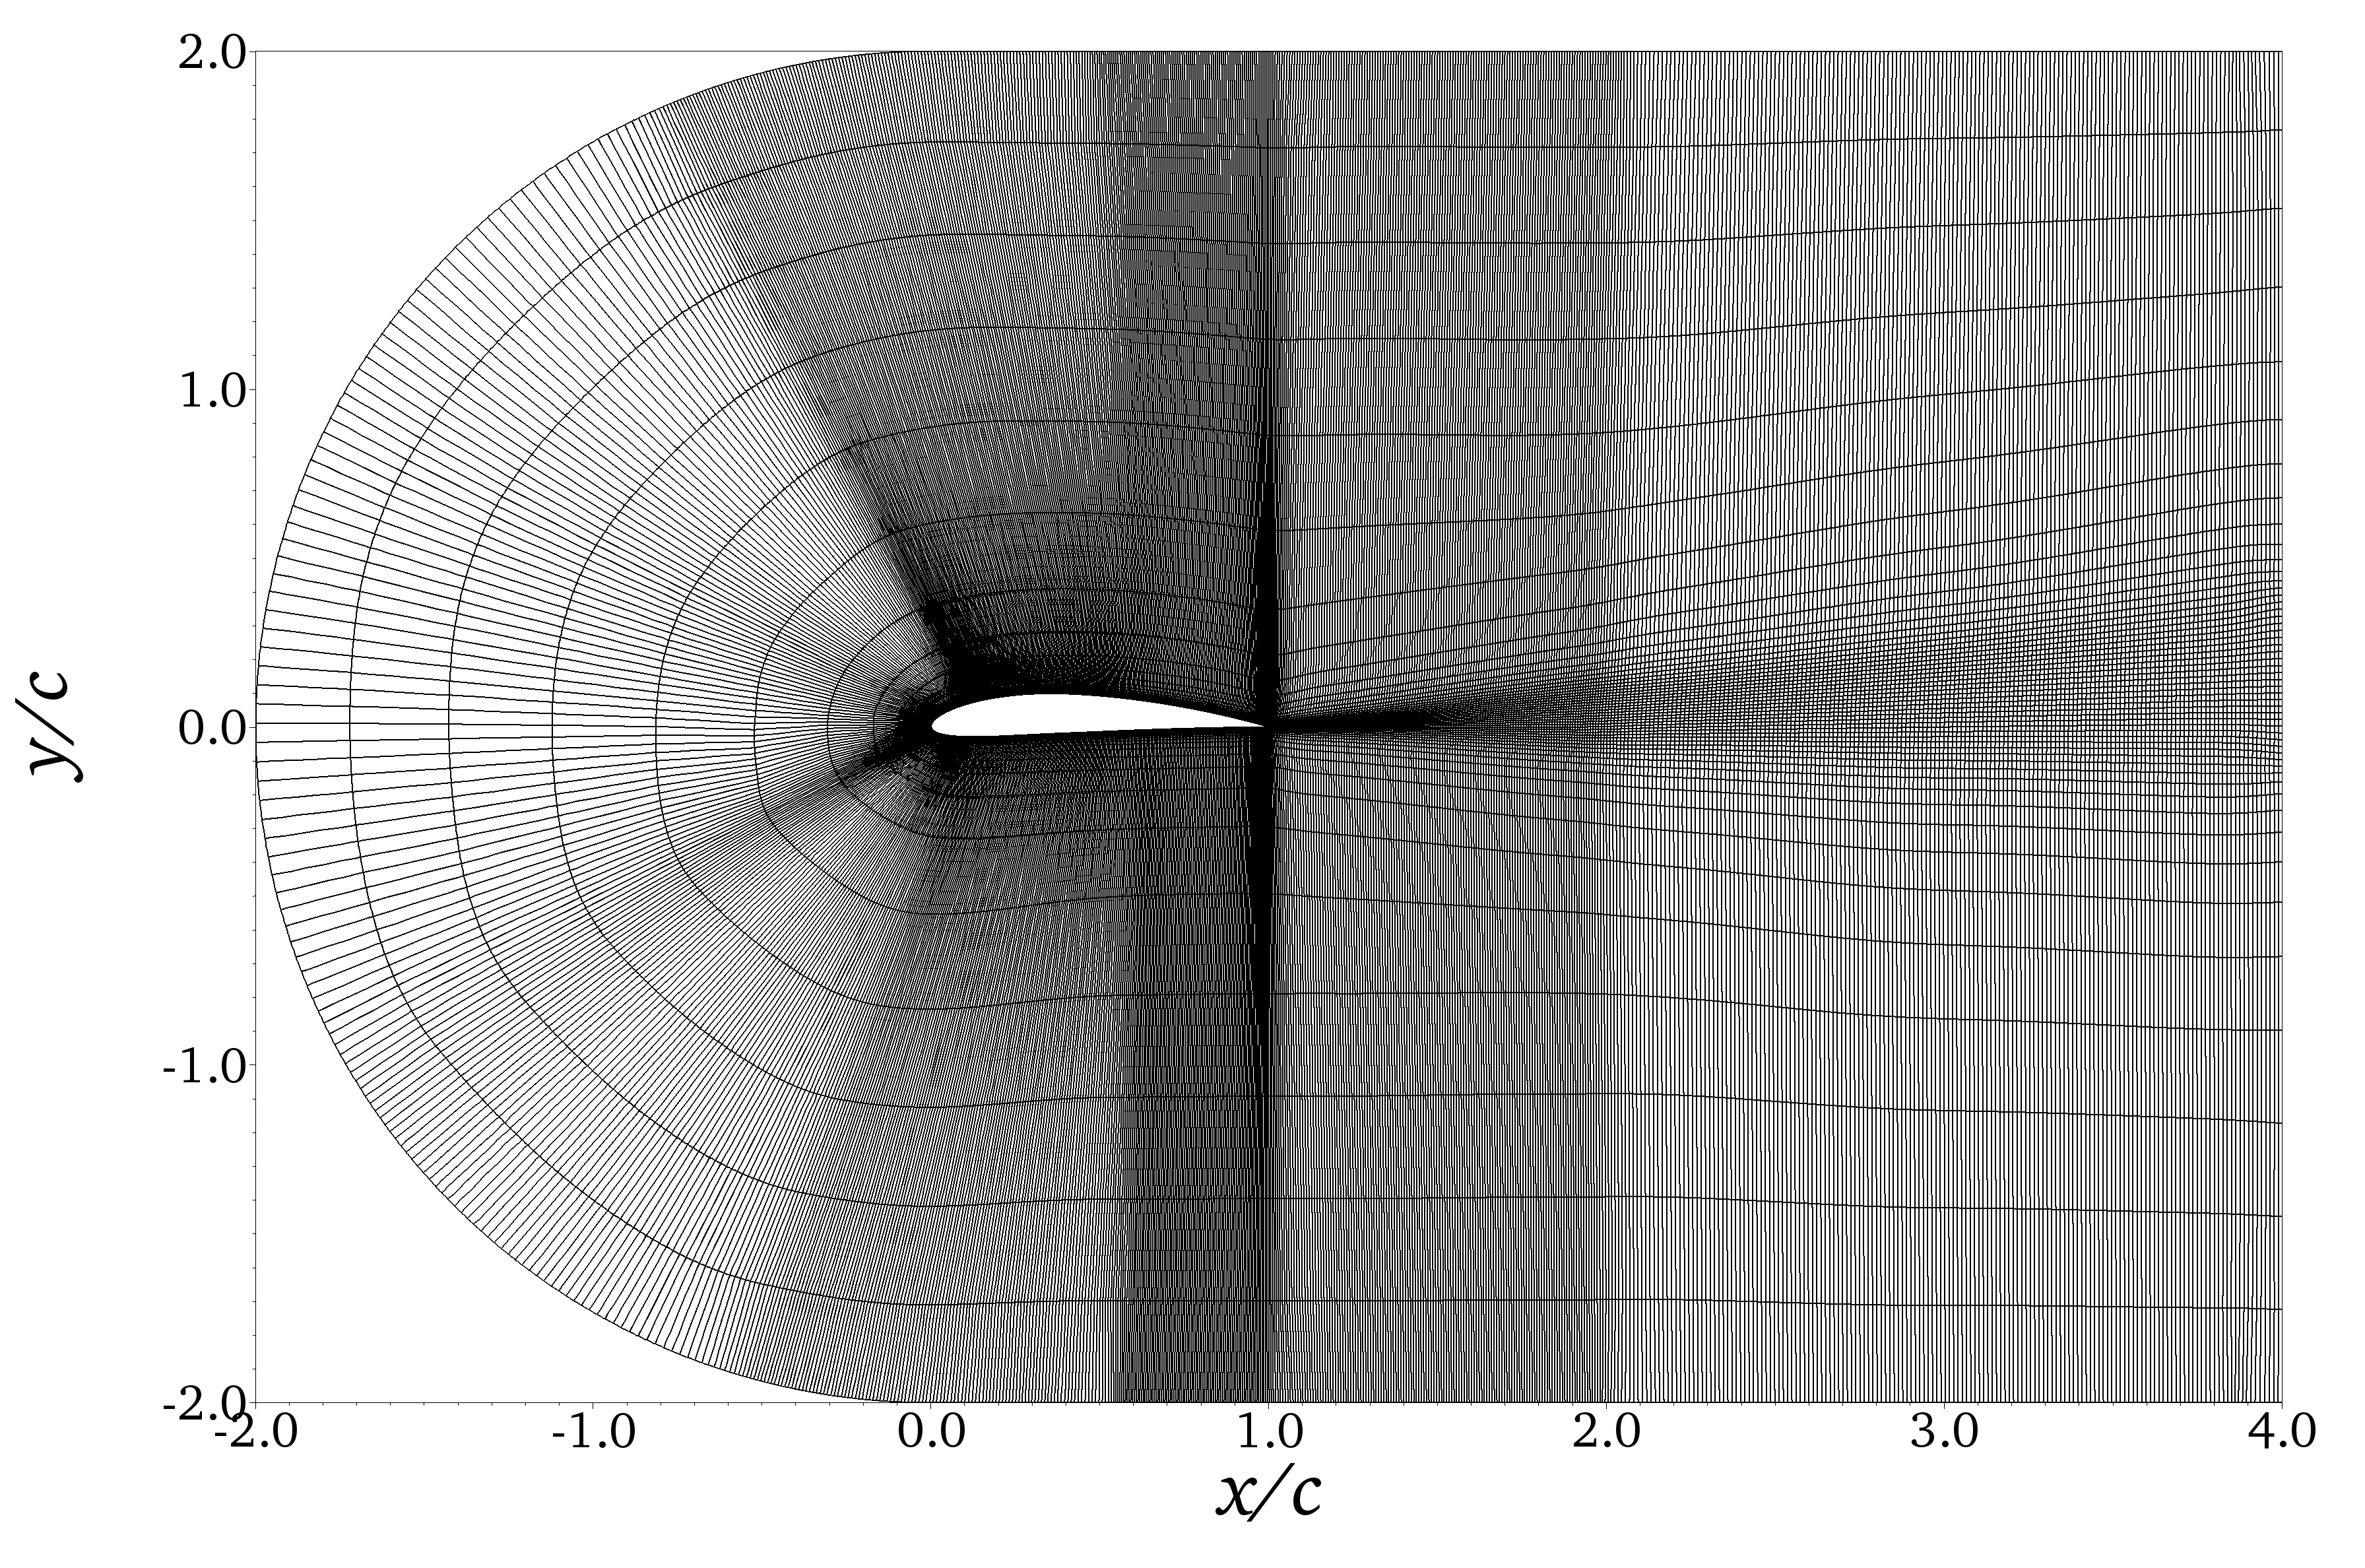
\includegraphics[width=0.49\textwidth]{paper4/imgs/wing_mesh}
	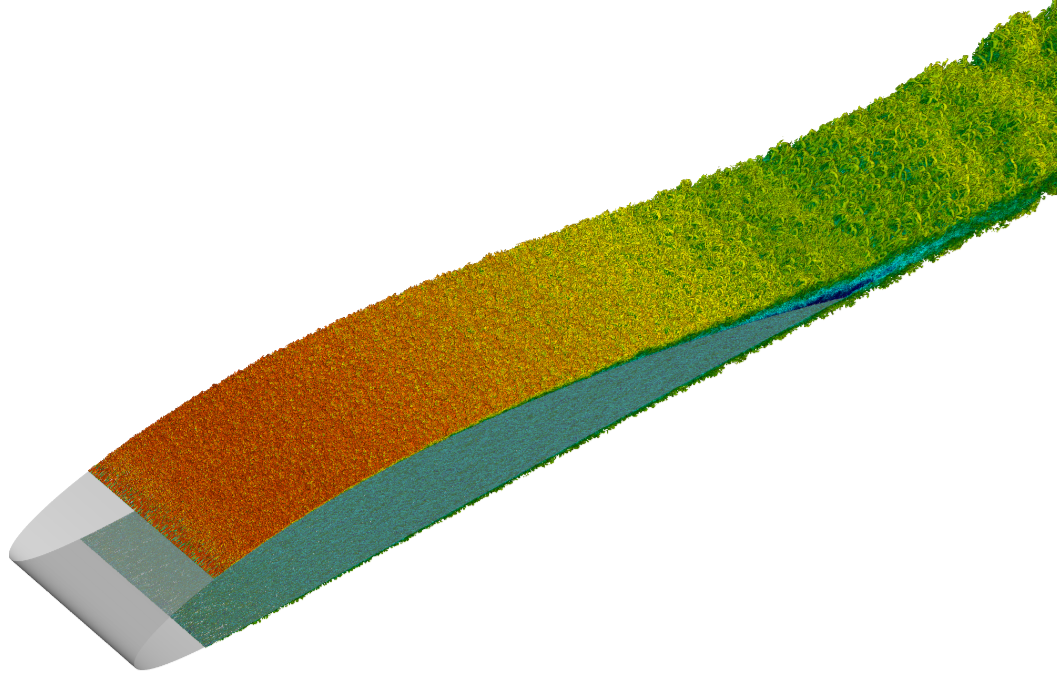
\includegraphics[width=0.49\textwidth]{paper4/imgs/wing_visualization}
	\caption{(Left) Two-dimensional slice of the computational domain showing the spectral-element distribution. (Right) Instantaneous flow field showing coherent structures identified with the $\lambda_{2}$ method \citep{jeong95}, and colored with horizontal velocity. In this figure, dark blue represents a horizontal velocity of $-0.1$ and dark red a value of $2$.}
	\label{fig:overview_flow_field_re1000k}
\end{figure}

\begin{figure}[t]
	\centering
	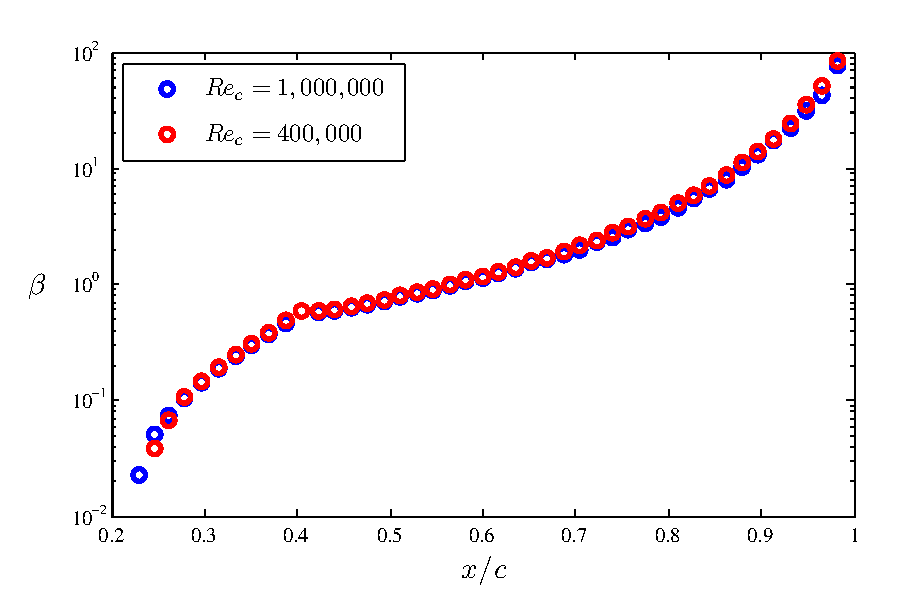
\includegraphics[width=0.49\textwidth]{paper4/imgs/beta_vs_x}
	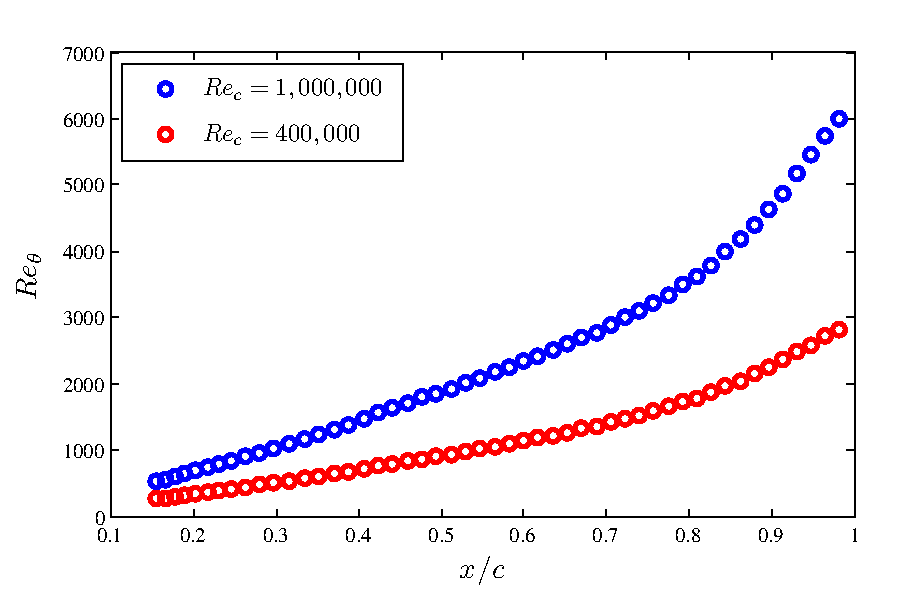
\includegraphics[width=0.49\textwidth]{paper4/imgs/Reth_vs_x}
	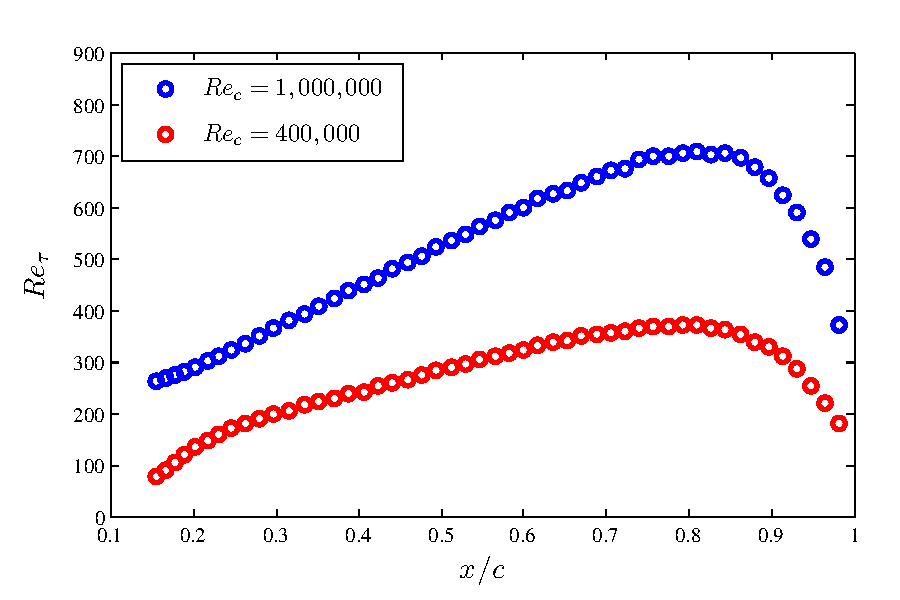
\includegraphics[width=0.49\textwidth]{paper4/imgs/Ret_vs_x}
	\caption{Streamwise evolution of (top left) the Clauser pressure-gradient parameter $\beta$, (top right) the Reynolds number based on momentum thickness $Re_{\theta}$ and (bottom) the friction Reynolds number $Re_{\tau}$, for the two wing cases under study.}
	\label{fig:overview_beta_Reth_Ret}
\end{figure}

%===============================================================================
\chapter{Conclusions and outlook}
%===============================================================================

The current thesis work concerns three different fields of research.

In the first part of the thesis, the ``evolve and filter'' technique for the stabilization of spectral-element methods is analyzed and it is found the filter operation causes an undesirable loss of divergence-free quality of the solution. This loss of divergence is shown to be particularly large for the test case of a double shear layer. An alternate formulation of the stabilization called the relaxation-term (RT) stabilization is shown to overcome the drawbacks of the explicit filtering technique, while maintaining the simplicity of the original explicit filter. This RT stabilization technique is very closely related to explicit filtering, with the two operations being equivalent to the leading order in time. Stability limits of the RT stabilization are explored and is shown to be stable within the practical parameter range.

In the second part, an NLF airfoil undergoing small-amplitude pitch-oscillations is analyzed at two different Reynolds numbers. In both cases a large variation of transition, and thus boundary layer characteristics is observed over the airfoil resulting in a non-linear response of the aerodynamic force coefficients. For $Re_{c}=750,000$ it shown that the temporal evolution of the transition point can be understood with a simple phase-lag concept, with the implication that boundary-layer evolution may be considered quasi-steady in time. Using this phase-lag concept a simple empirical model is developed which is able to explain a fairly wide range of experimental data.

On the other hand, for $Re_{c}=100,000$ a qualitatively different picture emerges for the unsteady boundary layer. The boundary-layer response displays a dynamically rich behavior with marked asymmetry of upstream and downstream transition movement. In this case, transition location is governed by the properties of the leading-edge laminar separation bubble (LSB) and it is conjectured that the absolute instability of the LSB may be responsible for abrupt changes in boundary layer characteristics.

Finally, in the third part of the study, flow over a stationary NACA 4412 airfoil is studied at two different Reynolds numbers with the aim of better understanding the boundary-layer evolution in non-equilibrium pressure gradient boundary layers. Two flow cases at a chord-based Reynolds number of $Re_{c}=400,000$ and $Re_{c}=1,000,000$ are compared at different streamwise locations. It is found that the effect of the streamwise pressure gradients is higher at low Reynolds numbers, leading to greater energy in the larger structures present in the outer part of the turbulent boundary layer.

The current work has laid the foundation for several interesting questions that may be the focus of future work. Can the simple empirical aerodynamic model be extended for a wider range of unsteady motions? Can the phase-lag be predicted a-priori as in the case of the classical model by \cite{theodorsen35}? When does the quasi-steady assumption break down and the boundary layer becomes truly unsteady? For $Re_{c}=100,000$, can the asymmetry of the (upstream and downstream) velocities of transition point be linked with the stability properties of the LSB? What is the influence of free-stream turbulence on unsteady LSB? In stationary airfoils, how does the velocity spectrum change with Reynolds number in non-equilibrium flows? What are the characteristics of boundary layer streaks in non-equilibrium flows? Some of these questions will be the focus of further research.


%===============================================================================
% Acknowledgments
%===============================================================================
%


\begin{acknowledgements}
	My foremost gratitude goes to my supervisor Dan Henningson for giving me the opportunity to join his research group. His knowledge and guidance have helped me immensely as a student. His encouragement, for which there is no substitute, have always provided the inspiration I needed to constantly push myself further in my work. Next I would like to thank my co-advisors Philipp Schlatter and Ardeshir Hanifi. Philipp for his patience during all my ignorant and sometimes foolish questions on numerics, conferences, papers and others that I probably can't recall. Ardeshir for the laughter, the sandwiches, the beers and most importantly, always being available on short notice when I needed help. I would also like to thank the members of the NFFP project, Roger Larsson, Dr. David Eller and Dr. Mikaela Lokatt for all the interesting discussions on aerodynamics. 
	
	I am grateful to Adam Peplinski for all the help he provided with Nek5000, MPI and coding in general. I can not imagine figuring out the workings of Nek5000 without his support. Armin and Ricardo have helped me more than others during my crucial time as a new Phd student. The help is greatly appreciated.
	
	Special mentions go to Mattias for all the coffee breaks, introducing me to Swedish food, the spontaneous discussions and being the bouncing board for all my (mostly wrong) ideas. Your company shall be missed once you leave the department. Jacopo and Giandomenico for all the great company, joining for the spontaneous plans and granting me the honorary Italian citizenship. I'll learn Italian very soon I promise! Marco for the constant dinner company. Freddy for the weekend food+beer+movie routine. Elektra for being one of the greatest friends of all time. Politics, late-night and of course Trump shall keep us entertained for times to come. But mostly, thanks for correcting my manuscripts and the support during this licentiate period. A mention must also go to my unrequited love, Walter Fornari. Where will I find another like you?
	
	A hearty thanks goes out to all my friends here at the department who make this a wonderful place. Eric, Clio, Nicolas, Sudhakar, Ugis, Evelyn, Anthony, Mehdi, Ali, Guillaume, Luca, Luca, Pierluigi, enrico, Francesco, Kristina, Ekatrina, J.C., Matthias, Priti, Ninge, Sagar, Krishne, Dhiya, and everyone else. All of you, with your quirks, jokes, stories and gossip (looking at you Pierluigi) add a little bit of color to life everyday.
	
	Perhaps most importantly, my deepest gratitude goes towards my family for their patience, unconditional love and support during my ever wandering path through life.
	
	Lastly, financial support for this work was provided by Vinnova through the NFFP project UMTAPS, with grant number 2014-00933, the Knut and Alice Wallenberg Foundation, and the European Research Council under grant agreement 694452-TRANSEP-ERC-2015-AdG.\ The computations were performed on resources provided by the Swedish National Infrastructure for Computing (SNIC) at the PDC Center for High Performance Computing at the Royal Institute of Technology (KTH). Simulation have also been performed at the Barcelona Supercomputing Center, Barcelona, with computer time provided by the $12^{th}$ PRACE Project Access Call (number 2015133182) and at the High Performance Computing Center, Stuttgart (HLRS) with the computer time provided by the $15^{th}$ PRACE Project Access Call (number 2016163965). 

\end{acknowledgements}



%===============================================================================
% References
%===============================================================================
%
\bibliographystyle{jfm}
\bibliography{licentiate}
%
\IfFileExists{overview.bbl}{\graphicspath{{imgs/}}
%\setlength{\captionmargin}{50pt}

%===============================================================================
\chapter{Introduction}
%===============================================================================
\section{A short history}

The first sustained flight by the Wright brothers in 1903 marked a historic day in human achievement and ingenuity. Momentous as the achievement was, the Wright brothers did not truly invent the modern airplane. Their achievements were the fruition of nearly a century of aeronautical research, starting perhaps with Sir George Cayley, who is considered the ``father of aerial navigation'' \citep{gibbs-smith62}. The principal components of the modern aircraft were laid down by George Cayley as early as 1799. Prior to Cayley, the ideas for mechanical flight tended towards flapping wings, where the flapping motion produced both propulsion and lift. George Cayley was the first to break the unsuccessful chain of thought and separated the two aspects of flight into distinct systems. His triple paper ``On Aerial Navigation'' published in Nicholason's \textit{Journal of Natural Philosophy, Chemistry and the Arts} on November 1809, February and March 1810 \citep{cayley1809} mark some of the most important works in aeronautical history. In the works, Cayley states for the first time, the principle of lift generation \textit{i.e.} the formation of a low pressure region on the upper surface of the wing. His paper elaborates on the separation of lift from propulsion and also goes on to talk about flight control and airplane stability. Later in his life, he proposed the concept of multiplanes (multiple wings mounted on top of each other) and built the first glider triplane named the ``boy carrier'' in 1849.

Several investigators followed the quest of ``aerial navigation''. Otto Lilienthal was the first to design and successfully fly controlled gliders in 1891, going on to make over $2500$ successful glider flights. Octave Chanute brought aeronautics research to America and designed a biplane glider which directly inspired the designs of the Wright Brothers. Samuel Pierpont Langley was a contemporary of the Wright brothers who built and tested several powered model airplanes. His success in achieving powered flight directly influenced and encouraged the Wright brothers. The final historic achievement of successful powered flight was achieved by the Wright brothers. On December $17^{th}$ 1903, a gasoline powered biplane by the name Wright Flyer I (figure~\ref{fig:wright_flight}) took flight in (modern day) Kill Devil Hills, North Carolina, ushering forth the era of practical human flight.
\begin{figure}[h]
	\centering
	\includegraphics[width=0.90\textwidth]{wright_brothers_first_flight}
	\vspace{10pt}	
	\caption{First flight of the Wright Flyer I, December 17, 1903, Orville piloting, Wilbur running at wingtip. Image from \cite{wikipedia_wright}.}
	\label{fig:wright_flight}
\end{figure}

\section{Modern aircraft design}
Since that fateful day, modern airplanes have been used in a variety of different conditions, varying from commercial passenger planes, to supersonic military aircrafts \citep{blackbird}, 
to endurance flights around the world lasting 9 days \citep{rutan_voyager}. The myriad uses have resulted in various challenges that need to be overcome by the aircraft designers. One significant challenge has been due to the dynamic interaction of air flow with the airplane structures, now studied under the field of aeroelasticity. These problems came to the fore as the design speed of aircrafts increased over the years and designers came to favor monoplanes over the biplane design. An early example was that of the Fokker D-8 German aircraft during World War I which suffered wing failure under steep dives, which was the first documented case of static aeroelastic effects.

Today the designers of commercial aircrafts face another challenge brought about by global climate change and rising oil prices. With the realization of the contribution of the aviation industry towards global climate change \citep{green08}, aircraft designers now face a need to significantly improve the fuel efficiency of commercial aircrafts in a bid to reduce the carbon footprint of the industry. In an effort to quantify the opportunities of achieving such an improvement, \cite{schrauf05} showed a break-down of the drag experienced by a typical transport aircraft highlighting that frictional drag accounted for more than half the drag experienced by the aircraft. Clearly a favorable modulation of the boundary layer over the wing could help achieve large improvements in fuel efficiency. The modulation could come in the form of effective flow control strategies, or with wing design strategies such as the use of natural laminar flow (NLF) airfoils. Both \cite{schrauf05} and \cite{green08} push forward the idea that NLF airfoils and laminar flow control strategies are the low-hanging fruits in the goal of higher fuel efficiency and a concerted effort into addressing the engineering challenges for practical implementation must be made. Some of these challenges may require revisiting the aeroelasticity problems from the perspective of laminar wings. However laminar flow at high Reynolds numbers is susceptible to destabilization and may not always be possible. Thus turbulent drag reduction strategies need to be used effectively where needed \citep{bushnell03}. Whatever the form of drag reduction technique that may finally be implemented on a particular aircraft, the understanding of developing boundary layers over wings (including the influence of control strategies) occupies a central position in aerodynamic research if the goal of higher fuel efficiency is to be realized. With this goal in mind, the current thesis work aims to further the understanding of developing boundary layers over airplane wings, focusing on two particular aspects.
\begin{itemize}
	\item Understanding the structure of the turbulent boundary layer developing over a wing section.	
	\item Understanding the evolution of the developing boundary layer over a natural laminar flow airfoil in unsteady flight conditions. 
\end{itemize}

%Solutions to these emerging aeroelastic problems needed an understanding of the unsteady phenomenon occurring in practical flight conditions. Such understanding came via the works of \cite{glauert30,karman38,theodorsen35} \textit{etc}, and by the 1940s, design engineers had the tools to account for unsteady aeroelastic effects in their wing designs.

%The achievements of these early aerdynamicists is quite impressive in particular considering that the boundary layer concept was in its nascent stages when the first practical airplanes were being designed. Indeed Prandtl's revolutionary concept of a boundary layer was first presented in 1904, almost a full year after the first flight of the Wright brothers.  

%-------------------------------------------------------------------------------
\section{Boundary layers over a stationary wing}

The understanding of the structure and scaling of wall-bounded turbulent flows has been in study for several decades and a complete understanding still remains far from complete. These flows have been studied with different canonical geometries such as channels \citep{kim87,moser99,lee15}, pipes \citep{elkhoury13,jimenez08,chin15} and flat plates \cite{spalart88,schlatter10,eitel14}. For the case of spatially evolving boundary layers over a flat plate, the simplest canonical case involves boundary-layer evolution subjected to a zero pressure gradient (ZPG). These flows may be uniquely characterized by a single parameter, \textit{i.e.} the Reynolds number Re, which is the ratio of the inertial and viscous scales of the flow. However practical flow cases are often influenced by pressure gradients. Such flow cases can no longer be uniquely defined using a single parameter. \cite{clauser54} with intuitive reasoning proposed a concept of an equilibrium boundary layer which may be uniquely defined by two parameters. He argued that, if the ratio of the average pressure gradient force across the boundary layer and the viscous shear force at the wall remains constant, the boundary layer would experience a similar flow history throughout its evolution. Thus the equilibrium pressure gradient boundary layers are uniquely defined by two parameters, namely the Reynolds number (Re) and the pressure gradient parameter $\beta$, defined as
\begin{eqnarray}
	\beta = \delta^{*}(dp/dx)/\tau_{w},
\end{eqnarray}
where $\delta^{*}$ is the displacement thickness, $dp/dx$ is the pressure gradient and $\tau_{w}$ is the wall-shear stress. The parameter is commonly referred to as the Clauser parameter. A flow case with a spatially constant Clauser parameter is categorized as an equilibrium boundary layer and a ZPG boundary layer is a special case of an equilibrium boundary layer with $\beta=0$. Several works have focused on pressure gradient boundary layers ranging from theoretical studies by \cite{townsend56,townsend56b,mellor66}, experimental works of \cite{skare94,harun13} and numerical simulations by \cite{spalart93,skote98}. The developing boundary layer over an airfoil however further increases in complexity since these boundary layers fall under the category of non-equilibrium boundary layers where the Clauser parameter is spatially varying. In such cases the flow history also plays a role in determining the local boundary layer properties \citep{clauser54,bobke17}. Analysis of such flow cases becomes significantly more difficult since the local boundary layer parameters do not uniquely define the state of the boundary layer. Nonetheless the study of such boundary layers is important since generic boundary layers found in nature would belong to this category, including the boundary layers over wings. The boundary layer developing over the NACA 4412 airfoil has the property that the spatially varying Clauser parameter is insensitive to Reynolds number. The presents us with the opportunity to study the Reynolds number effects of a non-equilibrium boundary layer with a constant pressure gradient history. That is indeed the methodology followed in this work. The developing boundary layer over a NACA 4412 wing section is analyzed at two different Reynolds numbers in order to understand Reynolds number effects in non-equilibrium boundary layers.

\section{Unsteady boundary layers}
%
Unsteady aeroydnamic studies started with the emergence of aeroelastic phenomenon in the early part of the $20^{th}$ century. With the gradual shift to monoplane designs, the inherent high torsional stiffness of biplanes was lost and aerodynamic instabilities, such as the one experienced by the Fokker D-8 became important. Pioneering works of \cite{glauert30,karman38,theodorsen35} \textit{etc}, provided the insight and modeling of such unsteady aerodynamic behavior and by the 1940s the foundations of unsteady aerodynamics for incompressible attached flows had been laid down. The mathematical framework these unsteady aerodynamic theories relied on simple inviscid and quasi-steady assumptions, which proved to be highly attractive to the wing designers \citep{leishman00}. Experimental corroboration by \cite{halfman52} and \cite{rainey57} further added support to the validity of the simple assumptions. Over the next few decades, investigations of unsteady aerodynamics shifted focus to the understanding of the dynamic stall phenomenon, with works of \cite{mccroskey76,mccroskey81,mccroskey82experimental,mccroskey82,carr1977,crisler94}. A large body of work on unsteady separated flows was presented by \cite{ericsson86,ericsson87b,ericsson_stall88a,ericsson_stall88b}. The studies continue to this day with the works of \cite{visbal11,visbal14,visbal17,dunne2015} and several other authors, a recent review can be found in \cite{coorke15}. 
\begin{figure}[h]
	\centering
	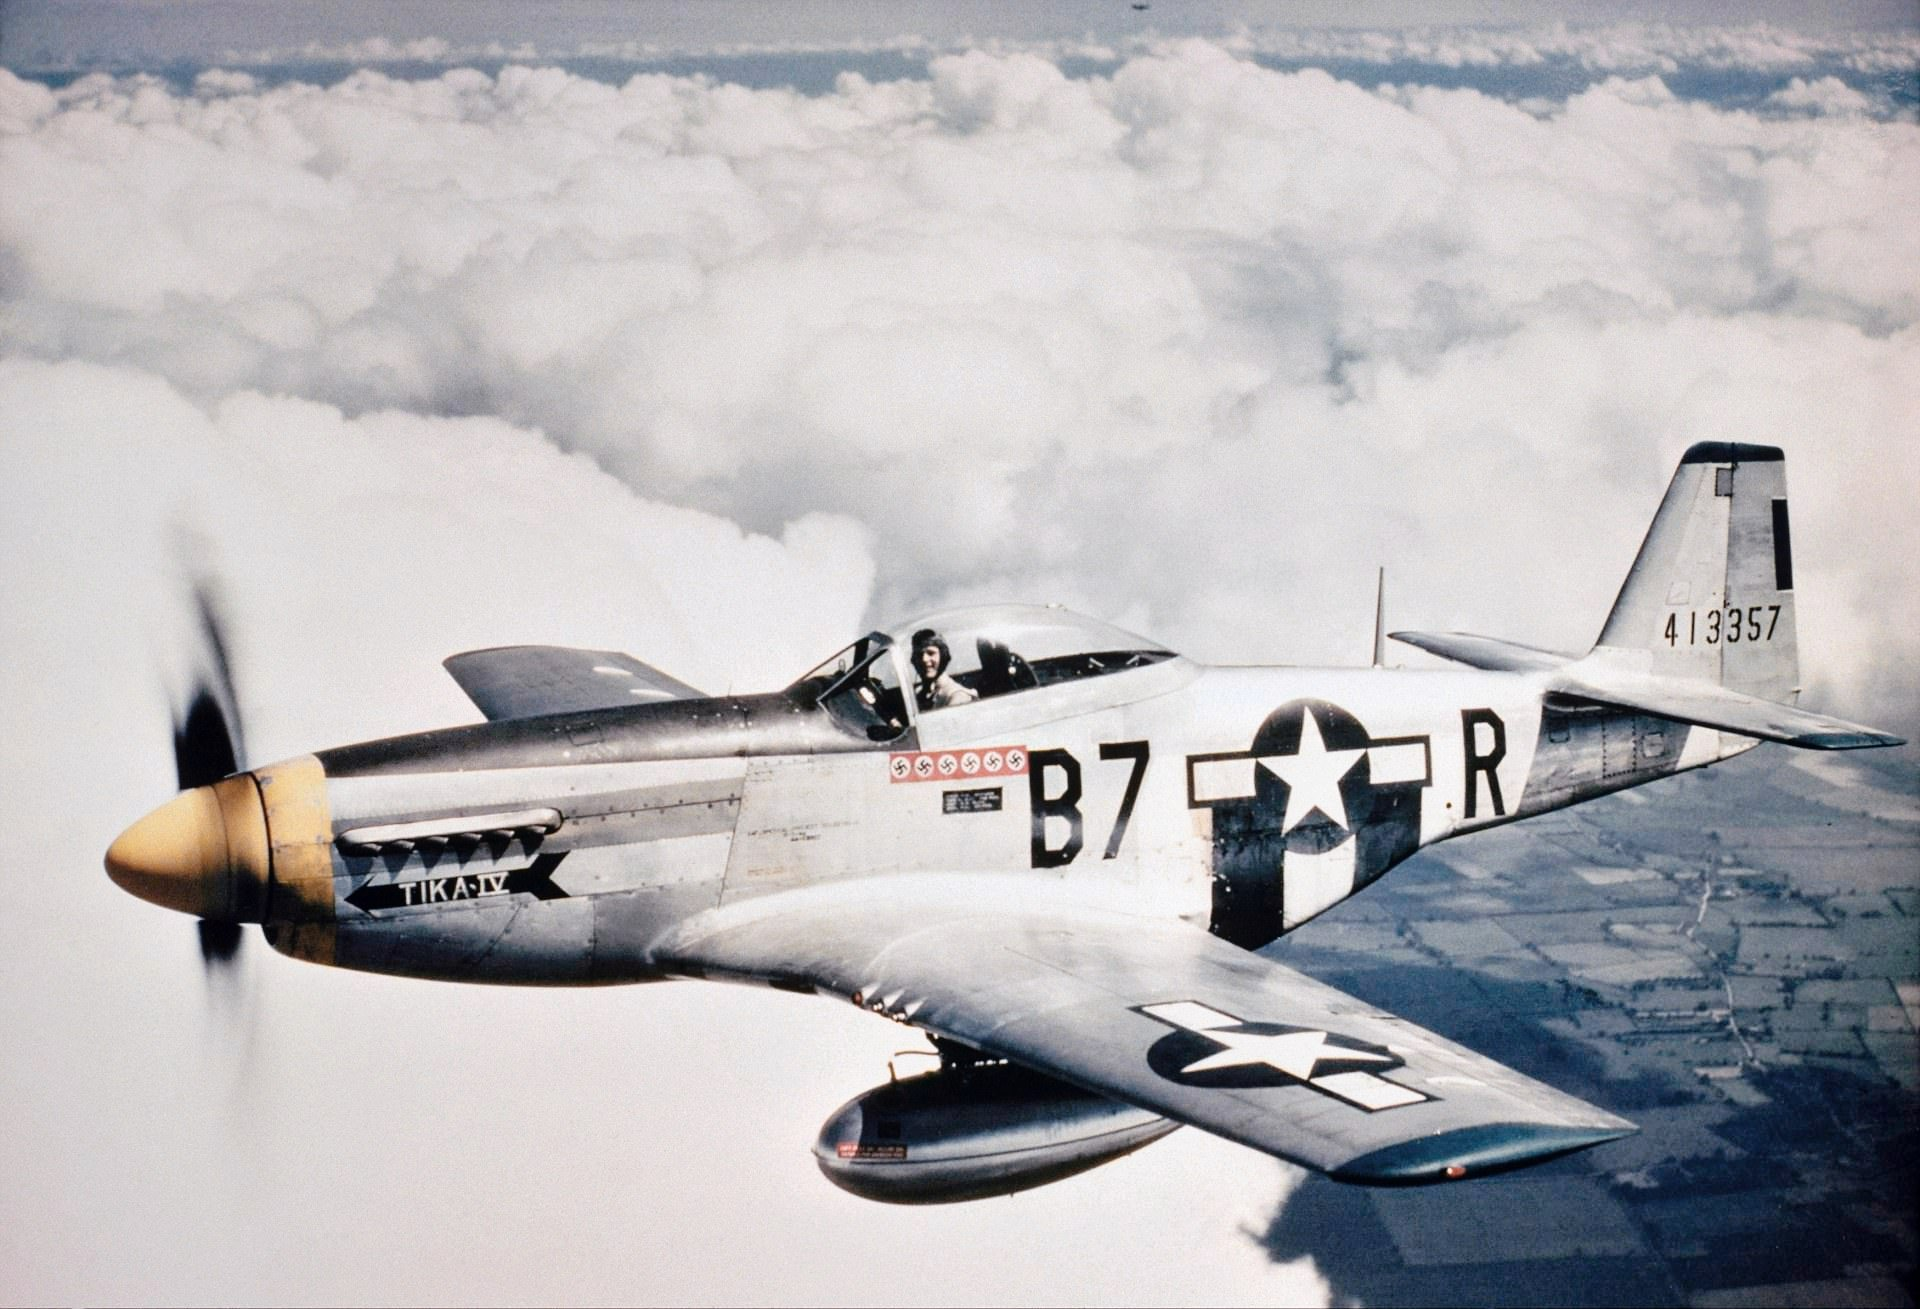
\includegraphics[width=0.90\textwidth]{P-51-mustang}
	\vspace{10pt}
	\caption{North American P-51 Mustang. Image from \cite{wikipedia_mustang}.}
	\label{fig:mustang}
\end{figure}

However it appears that the aeroelasticity problem was not considered from the perspective of natural laminar flow airfoils. This is a surprising fact considering the P-51 Mustang (figure~\ref{fig:mustang}), a fighter aircraft in the Royal Air Force designed in 1940, incorporated a wing with a natural laminar flow airfoil section \citep{green08}. The first aeroelastic study on laminar wings was performed as late as 2011 by \cite{mai11}. This, along with a subsequent investigation by \cite{hebler13}, brought to light a peculiar characteristic of unsteady laminar wings, \textit{i.e.} the presence of non-linearities in the unsteady aerodynamic forces. The classical unsteady aerodynamic theories did not predict non-linear unsteady responses and thus fail to account for such behavior. Inspired by this, \cite{lokattthesis} performed experiments on unsteady NLF airfoils and also found strong non-linearities in the aerodynamic forces. Consistent in the explanation for the non-linearities in all these studies was the role of transition over the wing surface. When transition on the airfoil suction-side was fixed (with a trip) near the leading edge, the non-linearities seemed to disappear. These results indicated a need for a more in-depth study of the evolving boundary layer in such unsteady laminar airfoils. Classical theories negate the role of the boundary layer by invoking the inviscid assumption and it is apparent that such an assumption is no longer be justified for laminar wings. Characteristics of the unsteady boundary layer are the subject of investigation in the present work.

\thesisstructure The thesis is structured as follows:
\begin{itemize}
	\item An overview of the numerical method used for the simulations is given in Chapter 2.
	\item Chapter 3 gives an overview of the numerical simulations performed in the study.
	\item The main conclusions of the current work are given in Chapter 4 along with an outlook for future work.
	\item The next part of the thesis includes the individual papers and internal reports. 
\end{itemize}

%===============================================================================
\chapter{Numerical Method}
%===============================================================================

\section{Numerical Discretization}

The numerical code used for the simulations is Nek5000, which is an open source research code developed by \cite{nek5000} at Argonne National Laboratory. The code solves the incompressible Navier--Stokes equations (\ref{eqn:navier_stokes}) in non-dimensional form:
\begin{subequations}
	\label{eqn:navier_stokes}	
	\begin{eqnarray}
	\frac{\partial u_{i}}{\partial t} + u_{j}\frac{\partial u_{i}}{\partial x_{j}} =  - \frac{1}{\rho}\frac{\partial p}{\partial x_{i}} + \frac{1}{Re}\bigg(\frac{\partial^{2} u_{i}}{\partial x_{j}\partial x_{j}}  \bigg) +f_{i} \\
	\frac{\partial u_{i}}{\partial x_{i}} = 0
	\end{eqnarray}
\end{subequations}
where $x_{i}$ is the coordinate direction, $u_{i}$ is the velocity component, $p$ is the pressure and $Re$ is the defined Reynolds number. The discretization of the Navier--Stokes equations is based on a spectral-element method, first proposed by \cite{patera84}. The method allows the mapping of elements to complex geometries along with a high-order spatial discretization within the elements, thus combining the generality of finite-element methods with the accuracy of spectral methods \citep{patera84}.
The spatial discretization in each element is performed following the $P_{N}$-$P_{N-2}$ \citep{maday89} formulation with velocity represented by high-order Lagrange interpolants through the Gauss--Lobatto--Legendre (GLL) quadrature points, while the pressure is represented on the staggered Gauss-Legendre (GL) quadrature points. The nonlinear terms are treated explicitly by third-order extrapolation (EXT3), while the viscous terms are treated implicitly by a third-order backward differentiation scheme (BDF3). Over-integration is used for the removal of aliasing errors. Nek5000 is written in Fortran 77 and C with efficient scaling for up to 1 million MPI ranks \citep{fischer15}.

%%%%%%%%%%%%%%%%%%%%%%%%%%%%%%%%%%%%%%%%%%%%%%%%%%%%%%%%%%%%%%%%%%%%%%
\section{Relaxation-term large-eddy simulation (RT-LES)}

Owing to the high Reynolds numbers and large time-scales of integration for some of the flow cases, a direct numerical simulation (DNS), which requires a resolution of all the spatial scales of the flow, leads to prohibitively high computational costs. In recent years a technique of wall-resolved large-eddy simulations has emerged as a computationally cheaper alternative to DNS, while also exhibiting the high-fidelity characteristics of DNS.
The technique has been utilized in the studies of spatially developing boundary layers \citep{eitel14}, pipe flows \citep{chin15} and flow over wings \citep{uzun10,lombard15}. The success of the approach has motivated its use in the present work. The wall-resolved LES method used is based on the RT3D variant of the ADM-RT approach first used by \cite{schlatter04}. The method has been shown to be reliable in accurately predicting transition and also preserving the characteristic structures which are seen in the DNS of transitional flows by \cite{schlatter06}. This particular quality of the LES model is crucial since there is a large focus on the unsteady transition in the present work. The LES method supplements the governing equations with a dissipative term $-\chi\mathcal{H}(u)$. The equations of motion for the resolved velocity and pressure thus read as
\begin{subequations}
	\label{eqn:rt_les}	
	\begin{eqnarray}
	\frac{\partial u_{i}}{\partial t} + u_{j}\frac{\partial u_{i}}{\partial x_{j}} =  - \frac{1}{\rho}\frac{\partial p}{\partial x_{i}} + \frac{1}{Re}\bigg(\frac{\partial^{2} u_{i}}{\partial x_{j}\partial x_{j}}  \bigg) + f_{i} -\chi\mathcal{H}(u_{i}), \\
	\frac{\partial u_{i}}{\partial x_{i}} = 0,
	\end{eqnarray}
\end{subequations}	
where $\mathcal{H}$ is a defined high-pass spectral filter and $\chi$ is a model parameter which together with $\mathcal{H}$ determines the strength of the dissipative term. The high-pass filter function $\mathcal{H}$ is defined such that the resultant relaxation-term only has energy in the highest modes, defined by a cut-off mode-number $N_{c}$. Figure~\ref{fig:filter_shape} illustrates the shape of the filter function in spectral space.
\begin{figure}[h]
	\centering
	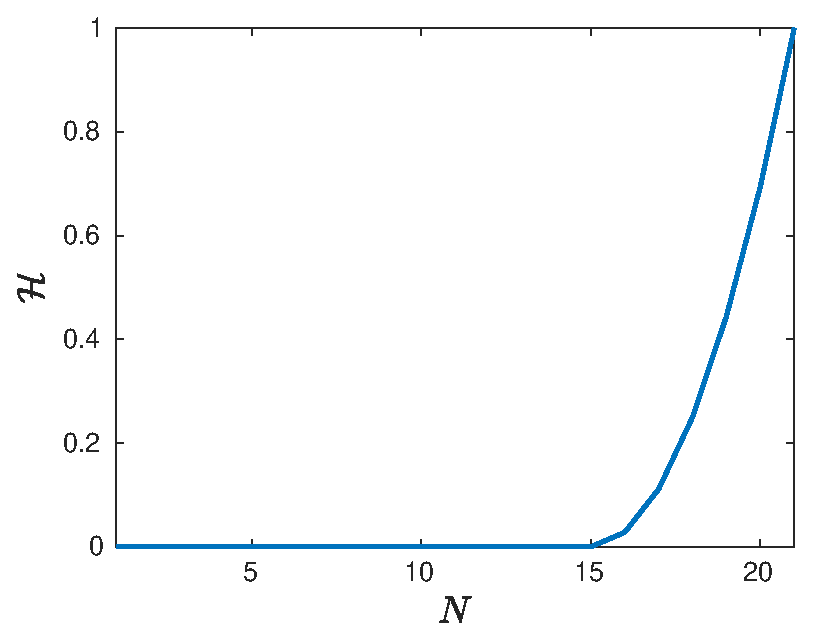
\includegraphics[width=0.60\textwidth]{filter_shape}
	\caption{Transfer function for the spectral coefficients for the filter $\mathcal{H}$ with number of modes $N=21$ and cut-off mode number $N_{c}=16$.}
	\label{fig:filter_shape}
\end{figure}

Several parameter optimization studies were performed to determine the optimum value of $\chi$ and filter shape $\mathcal{H}$ using turbulent channel flow simulations. The LES results were compared with the DNS database of \cite{moser99} and the optimum parameters were further validated for a flow around a wing section at $Re_{c}=400,000$. A good agreement was found between the LES and the DNS data of \cite{hosseini16}, and the optimized parameters were then used for all subsequent simulations.

\section{Arbitrary-Lagrangian-Eulerian (ALE)}

Typical solutions of unsteady fluid flows utilize the Eulerian framework where the coordinate system is fixed in space. A fixed coordinate system however becomes infeasible when the domain boundaries are in motion, as is the case of fluid-structure interaction problems, or when there is a free surface which may lead to a deforming interface. An appropriate method is needed to account or the motion of the boundaries and/or the interior grid points. One such method which substantially simplifies the difficulties arising out of moving boundaries is the Arbitrary-Lagrangian-Eulerian (ALE) method. The method was proposed in a finite-difference framework by \cite{hirt74} and later brought to the spectral-element framework by \cite{ho90,ho91}. The technique combines both the Lagrangian and Eulerian formulations such that, the Navier--Stokes may be solved with the grid points moving with the fluid elements \textit{i.e.} in a Lagrangian framework, or with fixed grid points (Eulerian), or with grid points moving in an arbitrary prescribed manner. The heart of the technique lies in the formulation of the total time rate of change of a quantity in the ALE frame, defined analogously to the material derivative. Thus for a quantity $\mathbf{F(x_{i},t)}$, the change due to small increments $dx_{i}$ and $dt$ may be expressed as \citep{kundu02}
\begin{align}
	dF = \frac{\partial F}{\partial t}dt + \frac{\partial F}{\partial x_{i}}dx_{i}.
	\label{eqn:material_deriv_df}
\end{align}
One may choose to follow any arbitrary path along which this quantity is evaluated, in which case the quantities $dx_{i}$ and $dt$ are related by the velocity of the (grid) point along this arbitrary path $w_{i} = dx_{i}/dt$. The relation results in the expression referred to as the ALE derivative \citep{deville02}, here denoted as $\delta F/\delta t$ to differentiate it from the very similar expression for the material derivative (which is evaluated along the fluid particle trajectory)
\begin{align}
\frac{\delta F}{\delta t} = \frac{\partial F}{\partial t} + w_{i}\frac{\partial F}{\partial x_{i}}.
\label{eqn:ale_derivative}
\end{align}
When $w_{i}$ is equal to the fluid velocity $u_{i}$, we recover the familiar Lagrangian expression for the material derivative $DF/Dt$. On the other hand, when $w_{i}=0$, we get the local (Eulerian) rate of change of the quantity $F$. The material derivative and the ALE derivative share a simple relationship defined using a relative velocity of the fluid particle with respect to the grid motion $c_{i} = u_{i} - w_{i}$, which may be used in the definition of material derivative to obtain
%\begin{subequations}
	\begin{align}
%	\frac{DF}{Dt} = \frac{\partial F}{\partial t} + u_{i}\frac{\partial F}{\partial x_{i}} \nonumber\\
%	\frac{DF}{Dt} = \bigg(\frac{\partial F}{\partial t} + w_{i}\frac{\partial F}{\partial x_{i}}\bigg) + c_{i}\frac{\partial F}{\partial x_{i}} \nonumber \\	
	\frac{DF}{Dt} = \frac{\delta F}{\delta t} + c_{i}\frac{\partial F}{\partial x_{i}}.
	\label{eqn:ale_material_derivative}
	\end{align}
%\end{subequations}
Thus the Navier--Stokes in the ALE formulation may be expressed as 
\begin{subequations}
	\label{eqn:ale_navier_stokes}	
	\begin{align}
	\frac{\delta u_{i}}{\delta t} + (u_{j} - w_{j})\frac{\partial u_{i}}{\partial x_{j}} =  - \frac{1}{\rho}\frac{\partial p}{\partial x_{i}} + \frac{1}{Re}\bigg(\frac{\partial^{2} u_{i}}{\partial x_{j}\partial x_{j}}  \bigg) +f_{i}, \\
	\frac{\partial u_{i}}{\partial x_{i}} = 0,
	\end{align}
\end{subequations}
where $w_{j}$ is the velocity of the grid points. The solution of the Navier--Stokes is then a simple matter of evaluating a suitable grid velocity. 

In many cases, such as the flow over an oscillating airfoil, the velocity of the grid points at the boundary (airfoil surface) may be explicitly known. \cite{ho90,ho91} propose to extend this velocity to the interior points of the domain by solving an elliptic problem for the mesh velocity. In the present work we take a simpler approach to prescribing the mesh velocities in the interior domain. Recognizing the simple trigonometric form of a harmonic pitching motion, all mesh points may simply be prescribed a solid body rotation with the instantaneous angular velocity of the airfoil. However a pure solid-body rotation would also displace the domain boundaries. Therefore a damping function is used to smoothly reduce the rotational velocity away from the airfoil boundary such that the mesh motion is zero at the far-field, inlet and outflow boundaries. Thus for an airfoil with an instantaneous rotation rate of $\Omega_{z}(t)$, the mesh velocity is prescribed as:
\begin{align}
	w_{i}(x,y,z,t) = \underbrace{(\Omega_{z}(t) \times \vec{R})}_{\text{Solid body rotation}} \overbrace{f(|\ \vec{r}\ |)}^{Damping}
	\label{eqn:mesh_velocity}
\end{align}
where $\vec{r}$ is the normal distance of a grid point from the airfoil surface, $\vec{R}$ is the distance from the rotational axis and $f(r)$ is a damping function which can be prescribed in many different ways, depending on one's preferences. The damping function needs to have two essential properties, \textit{i.e.} it must be equal to 1 when $|\vec{r}|=0$, which implies the mesh points at the airfoil boundary move with the surface (solid body rotation at the airfoil surface), and it must smoothly decay to zero close to the far-field boundaries, which allows the external boundaries of the computational domain to remain fixed in physical space. Figure~\ref{fig:mesh_rotation_damping} shows the damping function used in the present work as a function of the normal distance from the airfoil surface.
\begin{figure}[h]
	\centering
	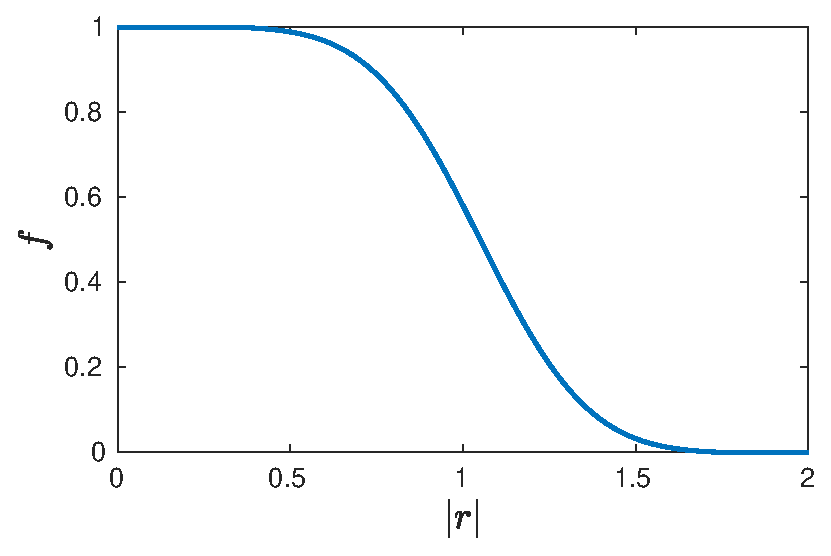
\includegraphics[width=0.55\textwidth]{damping_func}
	\vspace{5pt}
	\caption{Damping function $f(r)$ for the mesh velocities.}
	\label{fig:mesh_rotation_damping}
\end{figure}
The damping function moves the grid points close to the airfoil surface with the same rotational velocity of the airfoil and spreads out the mesh deformation into the interior of the domain. This damping function is calculated once at the beginning of the simulation. Hence all quantities $\Omega_{z}(t),\ \vec{r},\ f(r)$ which are needed for prescribing the mesh velocity are explicitly known at each time-step without the need for solving an elliptic equation as in \cite{ho90,ho91}. 

\section{Free-stream turbulence}

Isotropic, homogeneous free-stream turbulence is prescribed at the inlet and far-field boundaries to add small disturbances to the flow-field, which simulate the disturbances found in a wind-tunnel or in free-flight conditions. The free-stream turbulence is prescribed as a superposition of Fourier modes with a random phase shift. The maximum and minimum amplitudes of the wavenumber vector are prescribed quantities and are limited by the resolution of the spatial discretization and size of the domain respectively. The wavenumber space between the minimum and the maximum is divided into 20 concentric shells with each shell representing the amplitude of the three-dimensional wavenumber vectors lying on the shell. 20 points are randomly chosen on each shell with the location of each point representing the three-dimensional components of the wavenumber vector. Thus the free-stream turbulence is represented by a total of 400 fourier modes. Care is taken to avoid very small wavenumber components which result in wavelengths in physical space that are larger than the computational domain. The streamwise length scales are transformed to a temporal frequency by invoking Taylor's frozen turbulence hypothesis and using the local mean streamwise velocity at the inlet for the space-time conversion. The amplitude of the free-stream modes on each spherical shell is scaled using the von K\'arm\'an spectrum. Figure~\ref{fig:fst_duct} shows an instantaneous visualization of the streamwise velocities in a doubly-periodic duct flow case with high ($5\%$) free-stream turbulence intensity prescribed at the the inlet. Figure~\ref{fig:ti_decay} shows the spatial decay of turbulence intensity. After a small initial distance of adjustment from the inlet, the turbulence intensity decays as a power law. A very similar method for generating free-stream turbulence for simulations of flat-plate boundary layers is used by \cite{schlatterdiploma,brandt04,schlatter08} and more recently for wind turbine simulations by \cite{kleusberglicenciate}.

\begin{figure}[h]
	\centering
	\begin{subfigure}[t]{0.49\textwidth}
		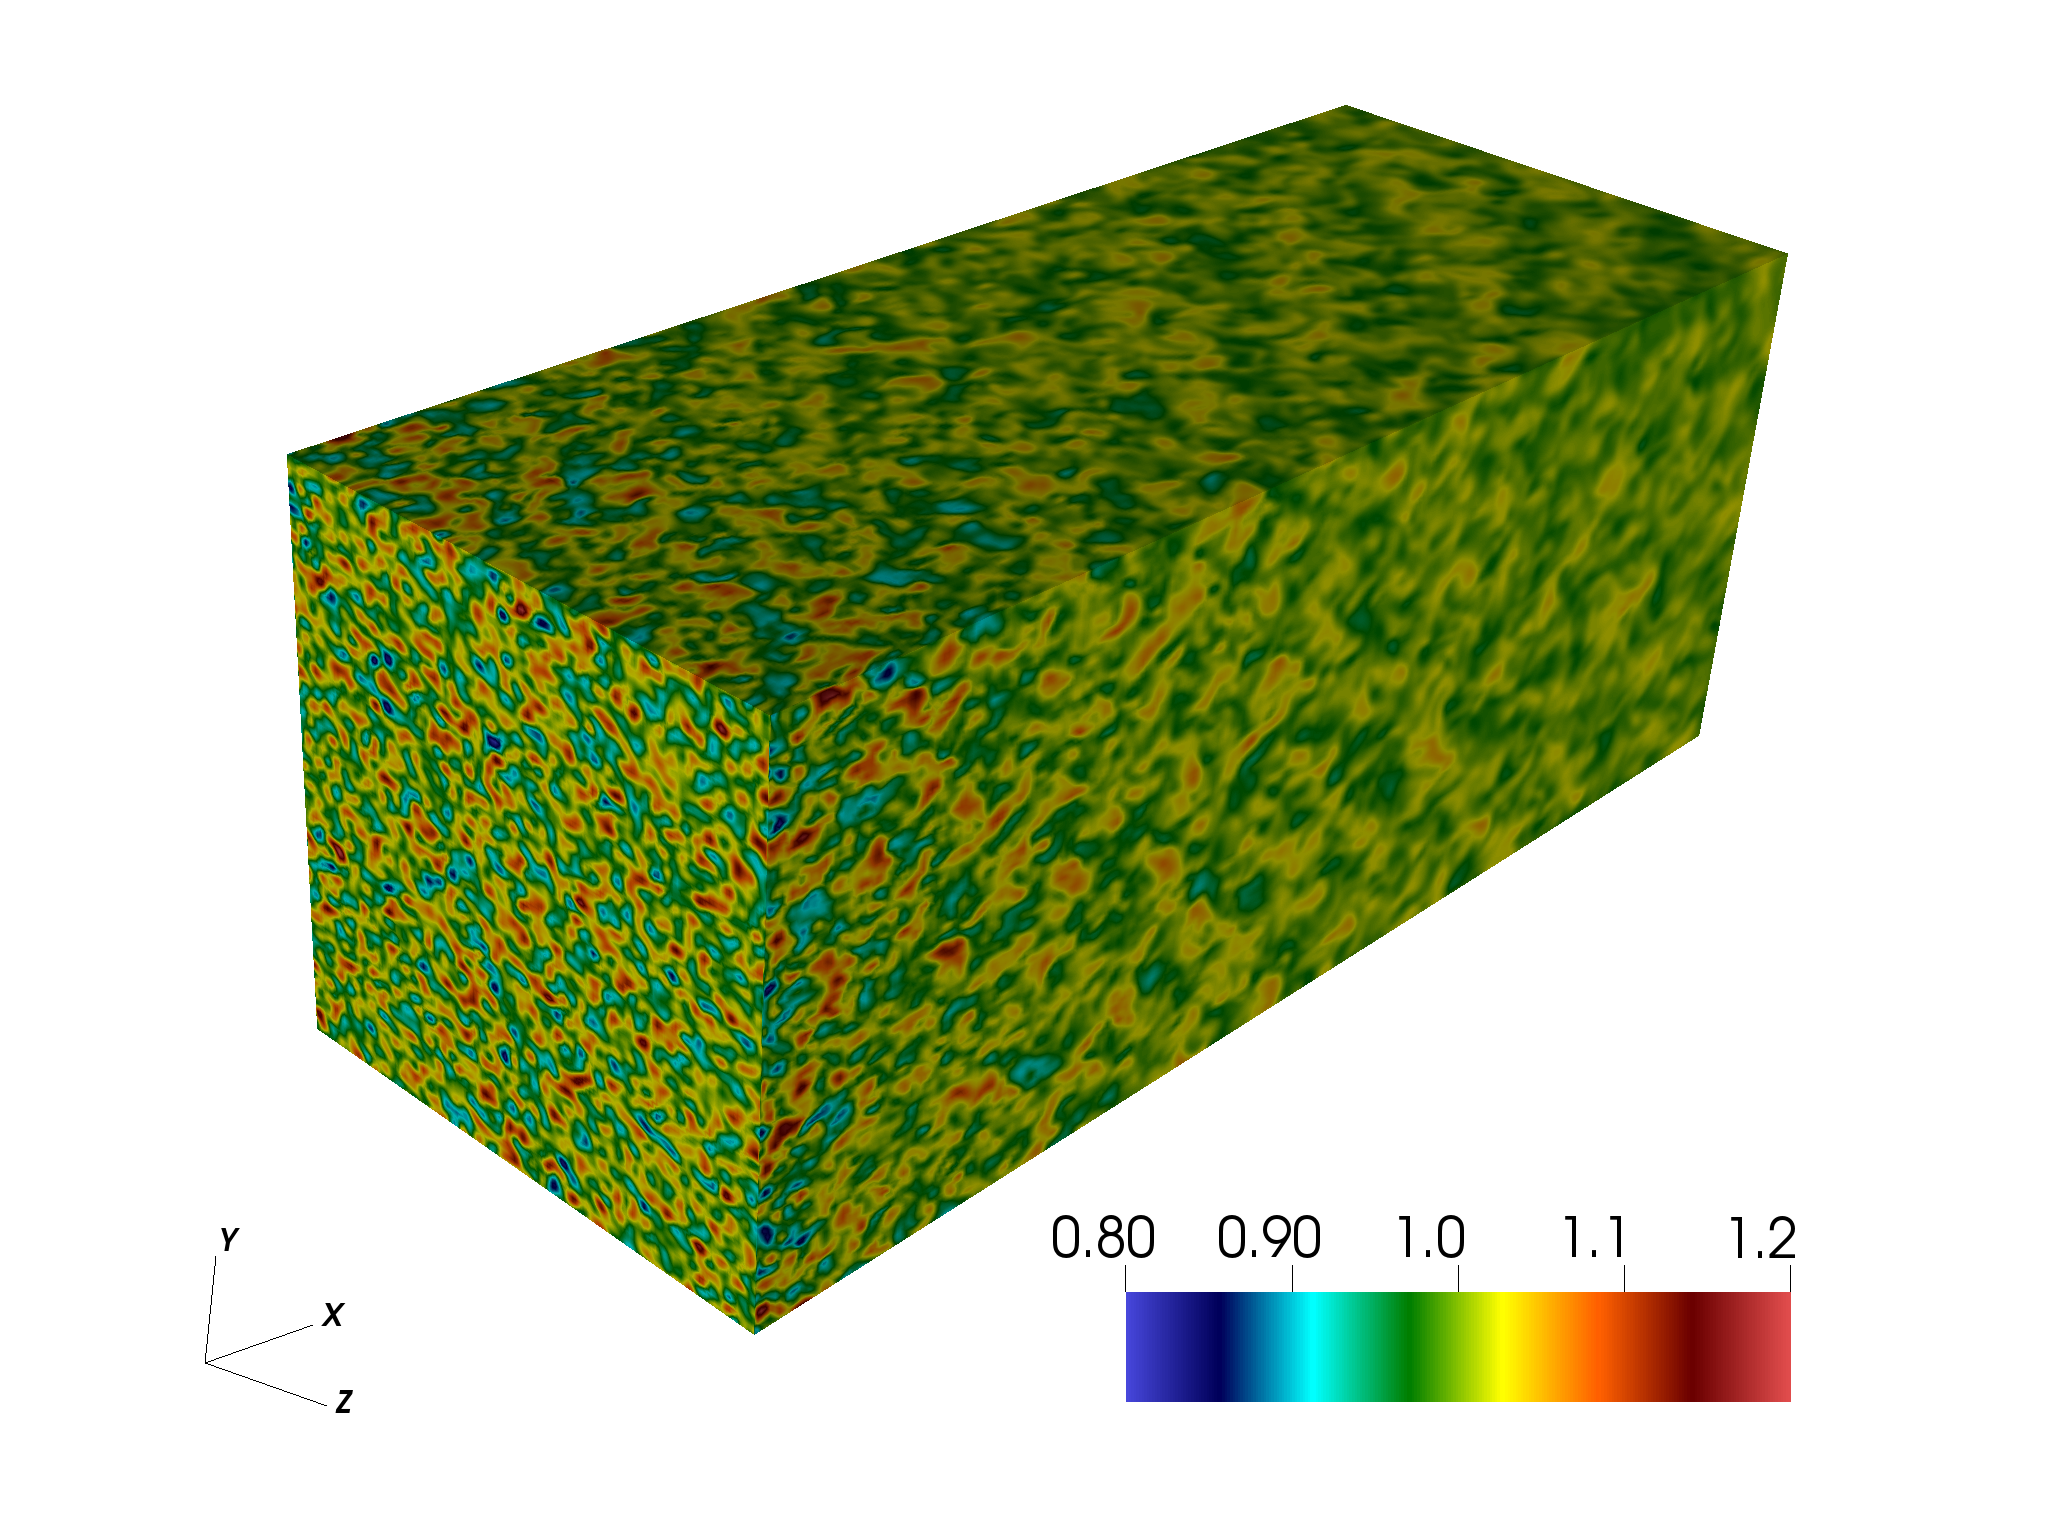
\includegraphics[width=1\textwidth]{fst_duct_vx0000.png}
		\caption{Visualization of free-stream turbulence prescribed at the inlet for a doubly periodic duct flow. Colors represent the instantaneous streamwise velocity.}
		\label{fig:fst_duct}
	\end{subfigure}
	\begin{subfigure}[t]{0.49\textwidth}
		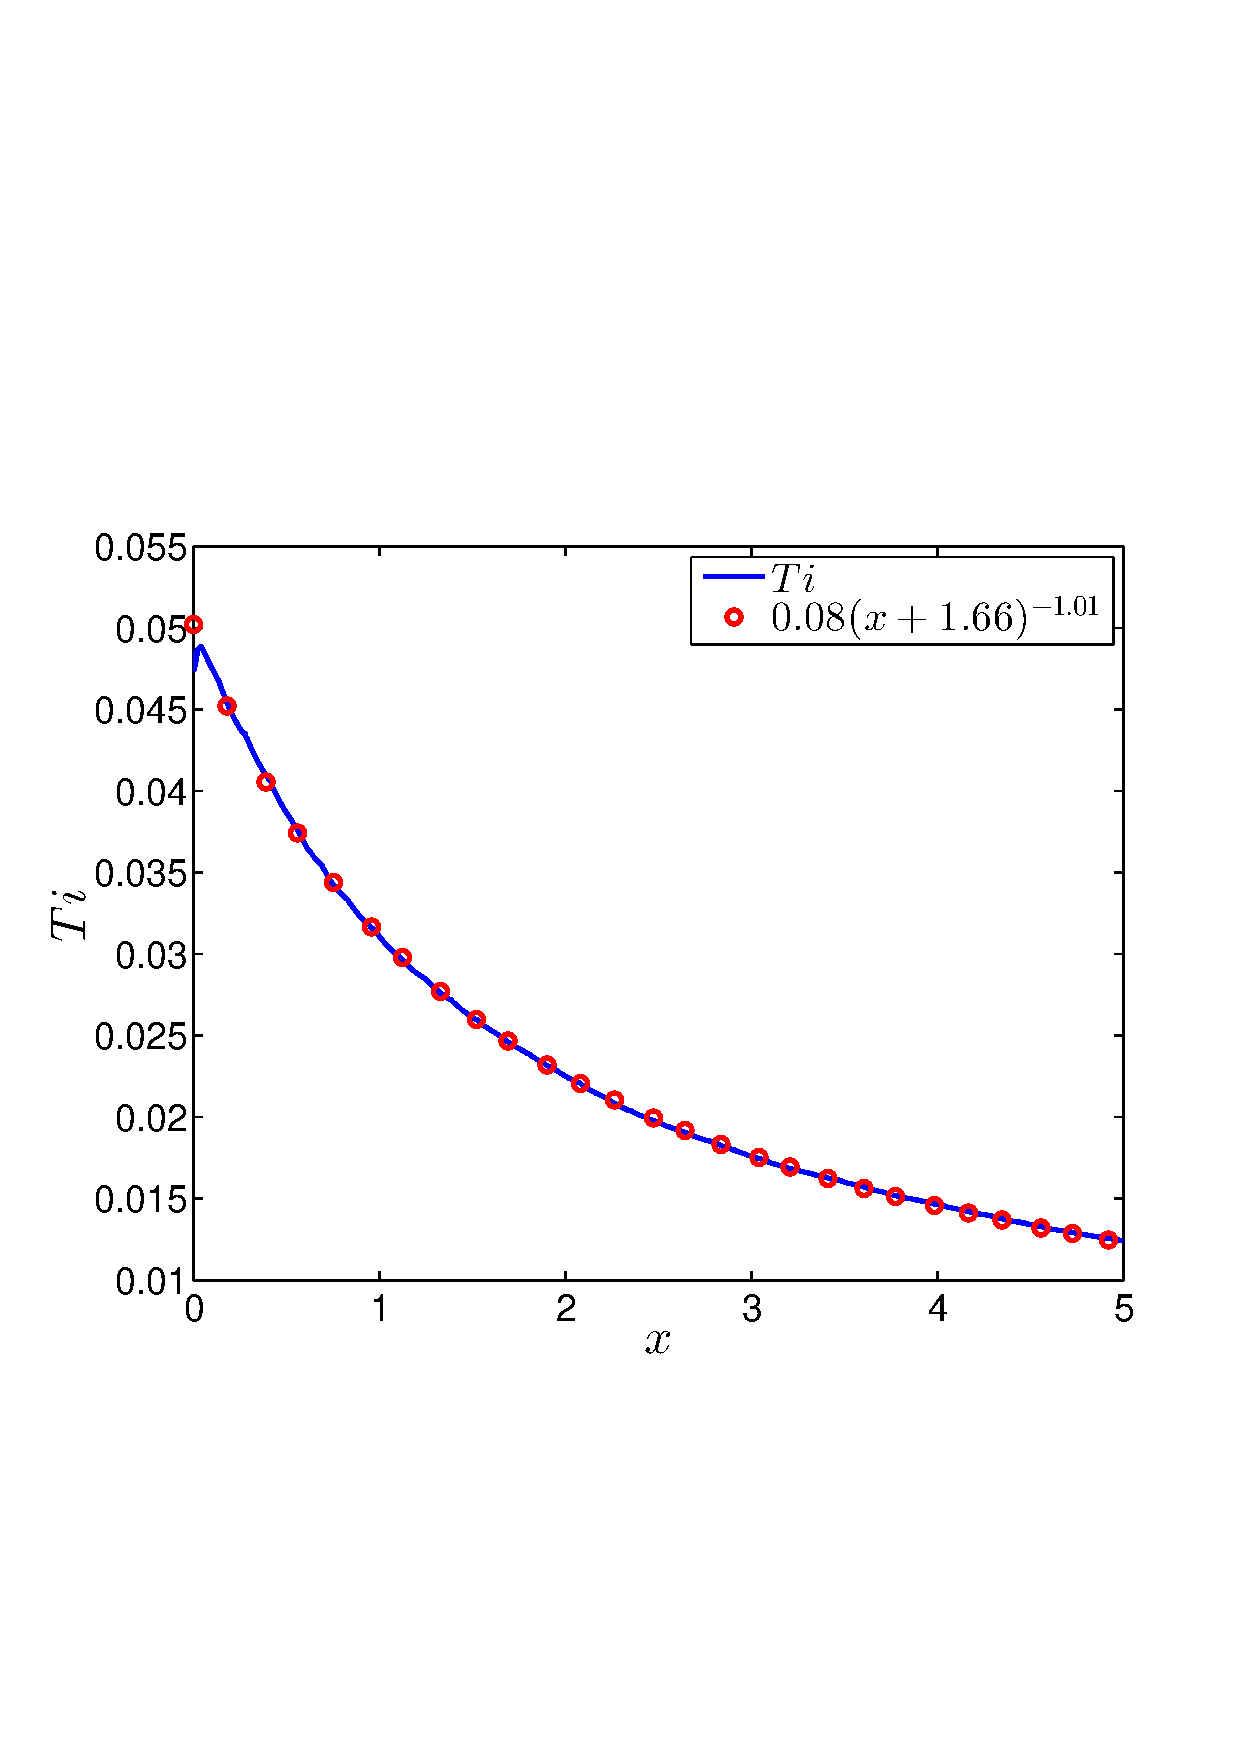
\includegraphics[width=1\textwidth]{ti_decay}
		\caption{Decay of turbulence intensity with streamwise distance, along with the least-squares fit of a power law.}
		\label{fig:ti_decay}
	\end{subfigure}
\end{figure}

%===============================================================================
\chapter{Overview of numerical simulations}
%===============================================================================

\section{Flow around unsteady wings}

The unsteady experiments of \cite{mai11,hebler13} and \cite{lokattthesis} have shown that aerodynamic non-linearities are related to the movement of transition over the suction side of the airfoil. Thus unsteady boundary layer dynamics play an important role in aerodynamic response of NLF airfoils. The present work investigates the unsteady boundary layers with a particular focus on unsteady transition with the aim to shed light on the phenomenon of non-linear unsteady aerodynamic response. The airfoil used in the investigation is the ED36F128 (with a $13.8^{\circ}$ flap deflection), designed at the Aeronautical and Vehicle Engineering department at KTH. It is a natural laminar flow airfoil, which has been used in several steady and unsteady experiments \citep{lokatt17,lokattthesis}. The unsteady experiments have shown the non-linearities that appear to be typical of laminar airfoils \citep{lokattthesis}. The results of the steady and unsteady experiments using this airfoil have been made available to us by Dr. Eller and Dr. Lokatt. Non-linearities in the unsteady aerodynamic forces are observed for only a certain range of angle of attack $\alpha$. Therefore a careful assessment of the data was needed in order to select the right parameter range where the relevant flow physics could be observed in the numerical simulations. The data in the experimental campaign was gathered primarily through pressure taps located around airfoil for the calculation of unsteady aerodynamic forces. Thus measurements of the unsteady boundary layer characteristics was not available through the experimental data. Calculations using an integral boundary layer code XFOIL \citep{drela89}, were used to complement the experimental data and better evaluate the state of the boundary layer in the static measurements.

Figure~\ref{fig:tr_xfoil_100_750} shows the calculated transition locations for two different Reynolds numbers ($Re_{c}=100,000$ and $Re_{c}=750,000$) using XFOIL and figure~\ref{fig:765k_static_cz_foil} shows the experimentally measured normal force coefficient as well as calculations from XFOIL for $Re_{c}=750,000$. For the higher Reynolds number case, transition location varies sharply with angle of attack within the range $3.4^{\circ}<\alpha<6.5^{\circ}$. Aerodynamic non-linearities can also be observed approximately within the same angle of attack range (figure~\ref{fig:765k_static_cz_foil}). For the lower Reynolds number case, no experimental data is available. Therefore solely XFOIL calculations are used and the parameter range is selected where the transition location varies rapidly with angle of attack. This is found for an angle of attack range of $6.7^{\circ}<\alpha<8.0^{\circ}$.
\begin{figure}[!h]
	\centering
	\begin{subfigure}[t]{0.45\textwidth}
		\caption{}
		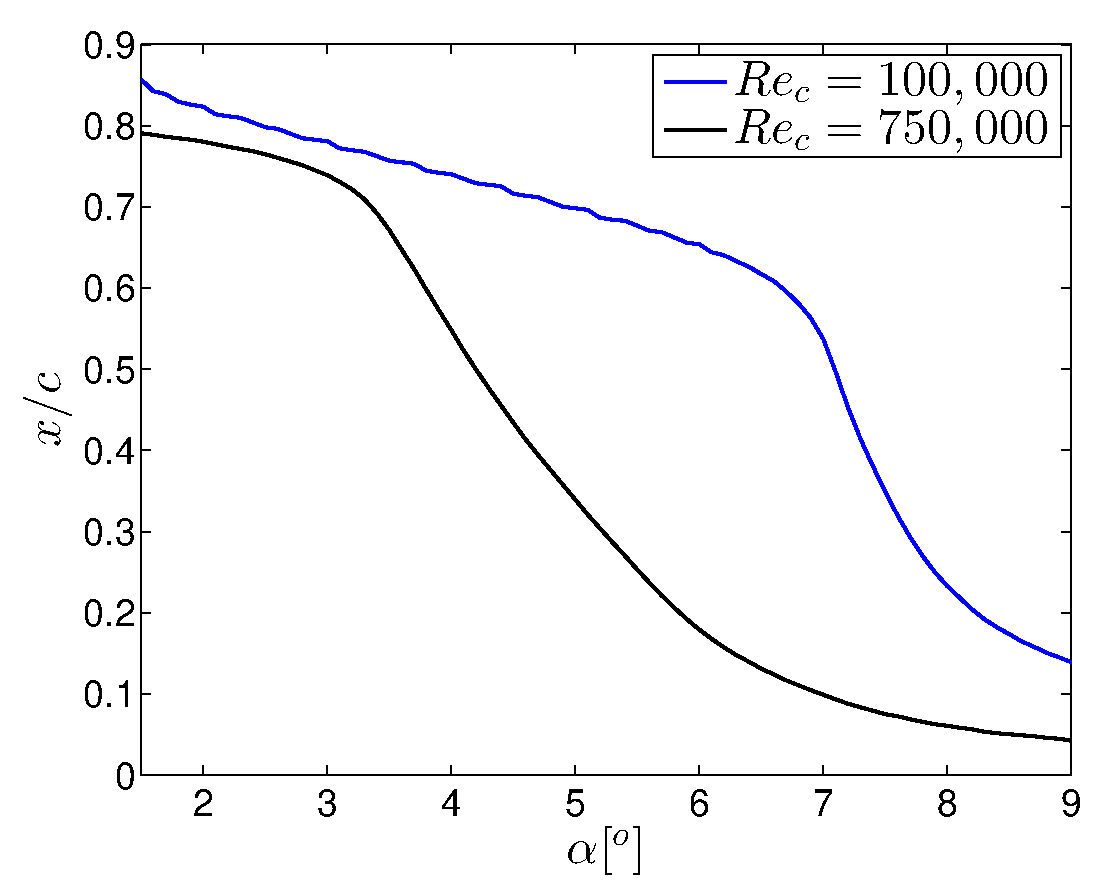
\includegraphics[width=1\textwidth]{tr_xfoil_100_750}
		\label{fig:tr_xfoil_100_750}		
	\end{subfigure}
	\begin{subfigure}[t]{0.45\textwidth}
		\caption{}
		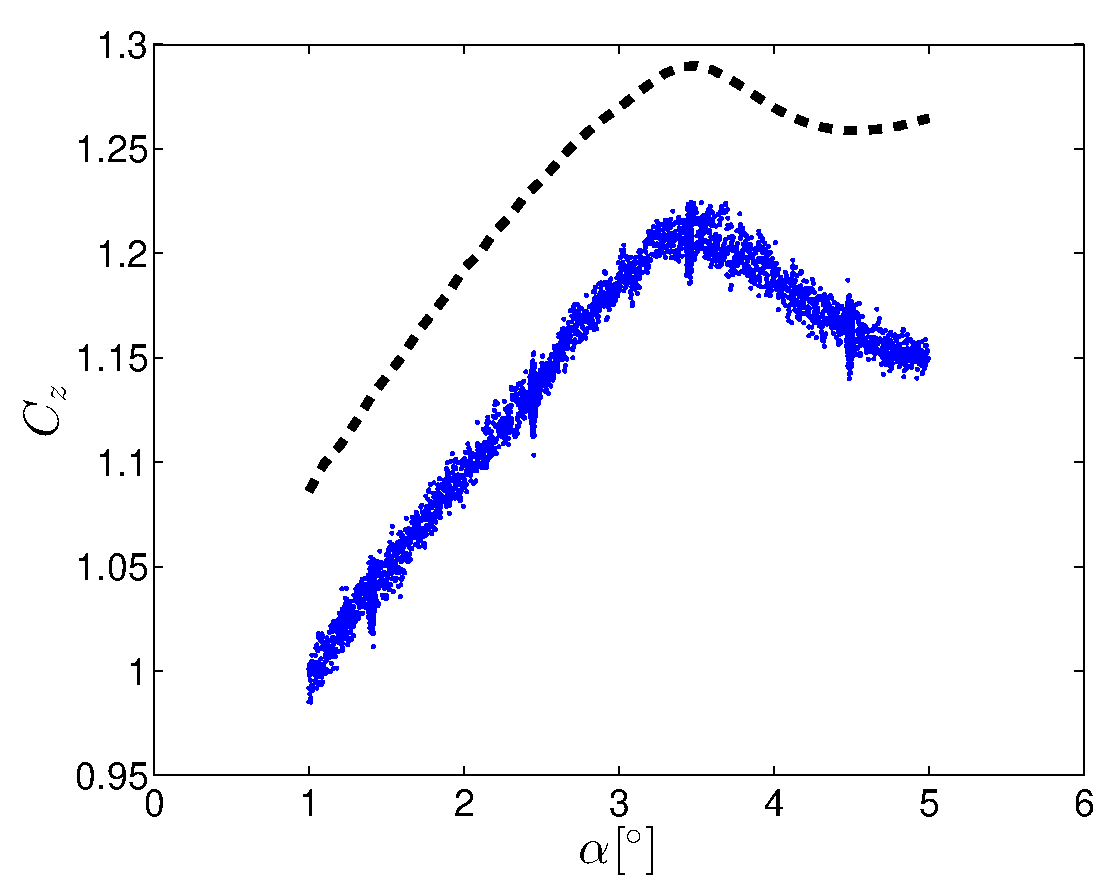
\includegraphics[width=1\textwidth]{765k_static_model_cz_xfoil}
		\label{fig:765k_static_cz_foil}
	\end{subfigure}
	\caption{(a) Transition location calculated using XFOIL for two different Reynolds numbers. (b) Normal force coefficient measured in experiments (dots) and from XFOIL calculations (dashed line) for $Re_{c}=750,000$.}		
\end{figure}
Numerical simulations are performed with stationary airfoils to ensure the expected static boundary layer characteristics are captured by the numerical simulations.  Figure~\ref{fig:overview_la2_750k_stationary} depicts the instantaneous vortical structures in the flow for $Re_{c}=750,000$ for an angle of attack $\alpha=2.4^{\circ}$ and $\alpha=4.4^{\circ}$ which shows the change in boundary layer characteristics in the static cases. Similarly, figure~\ref{fig:overview_isocontour_aoa} shows the static boundary layer characteristics for $Re_{c}=100,000$ at $\alpha=6.7^{\circ}$ and $\alpha=8.0^{\circ}$.
\begin{figure}[h]
	\centering
	\begin{subfigure}[t]{0.49\textwidth}
		\caption{$\alpha=2.4^{\circ}$}		
		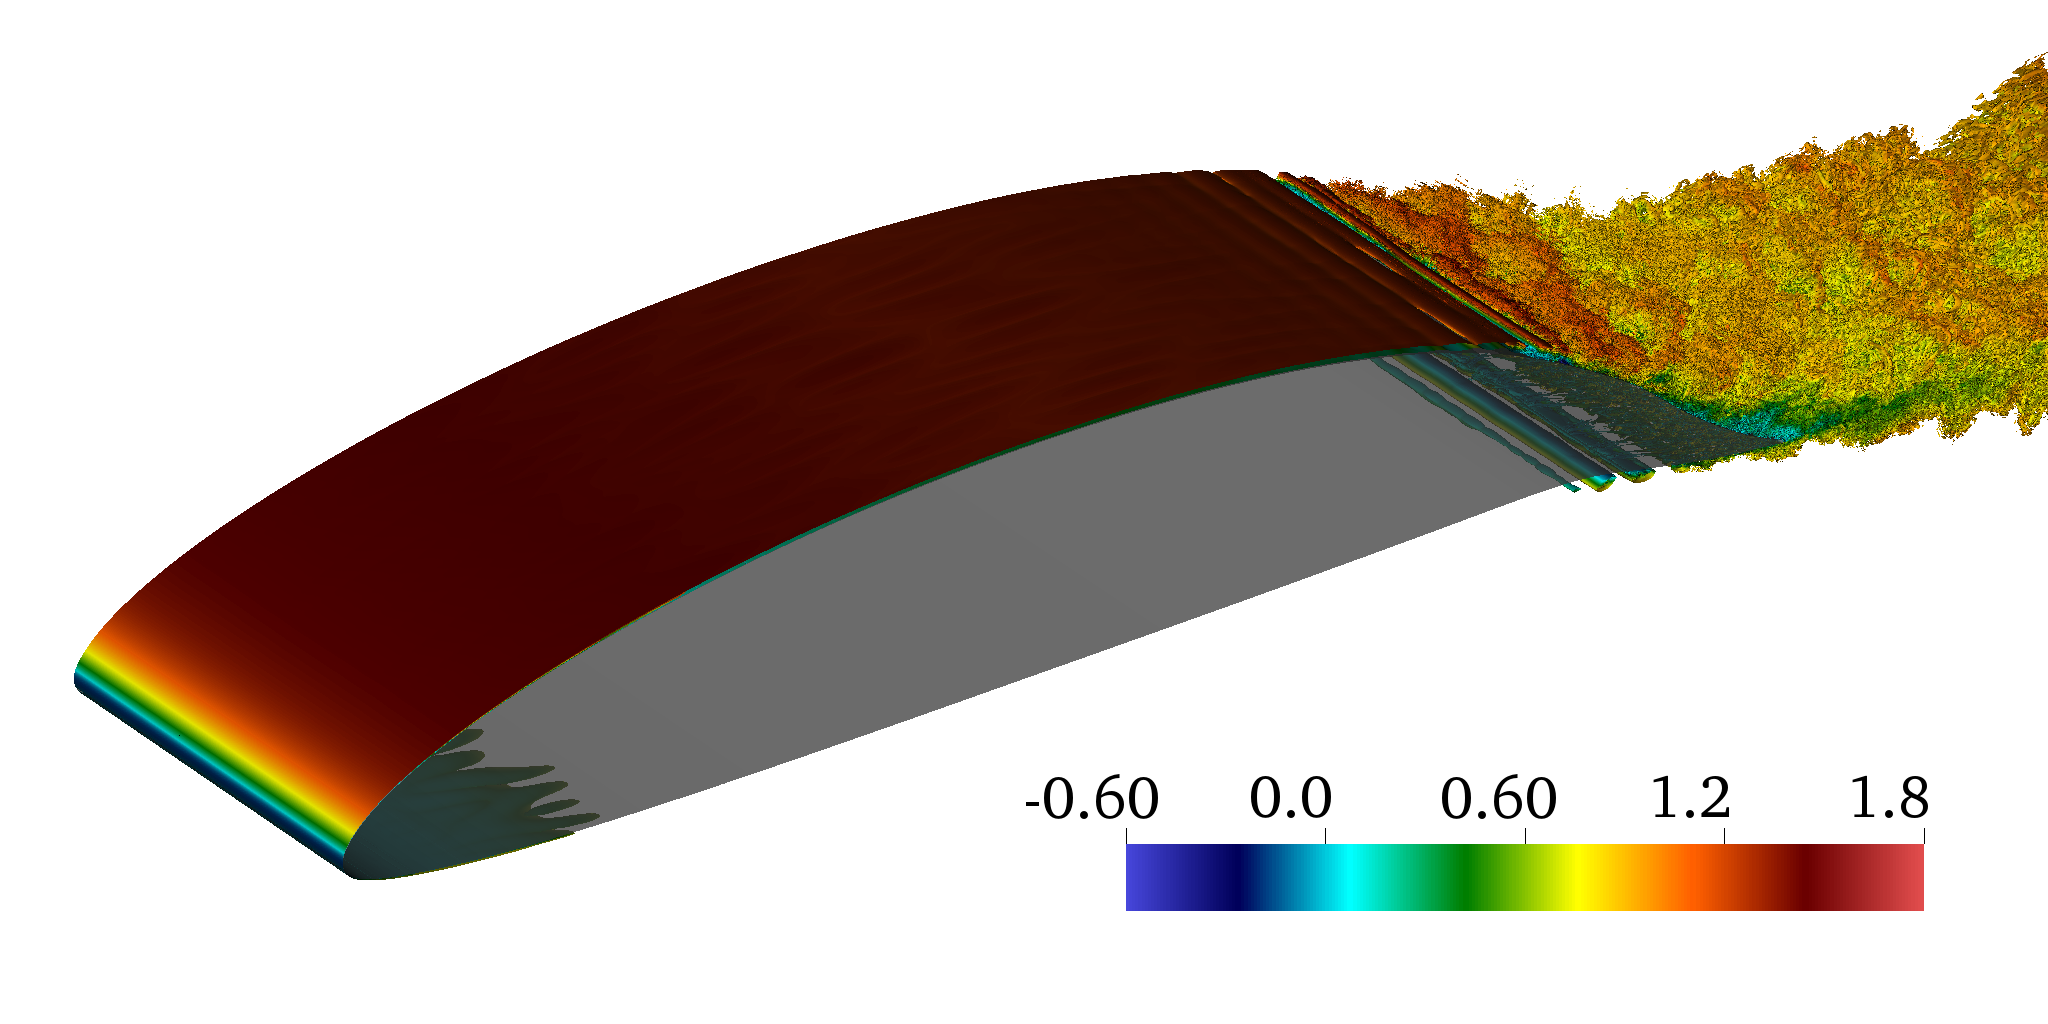
\includegraphics[width=1\textwidth]{paper2/imgs2/pitch_re750k0001}
		\label{fig:overview_la2_aoa24}
	\end{subfigure}
	\begin{subfigure}[t]{0.49\textwidth}
		\caption{$\alpha=4.4^{\circ}$}		
		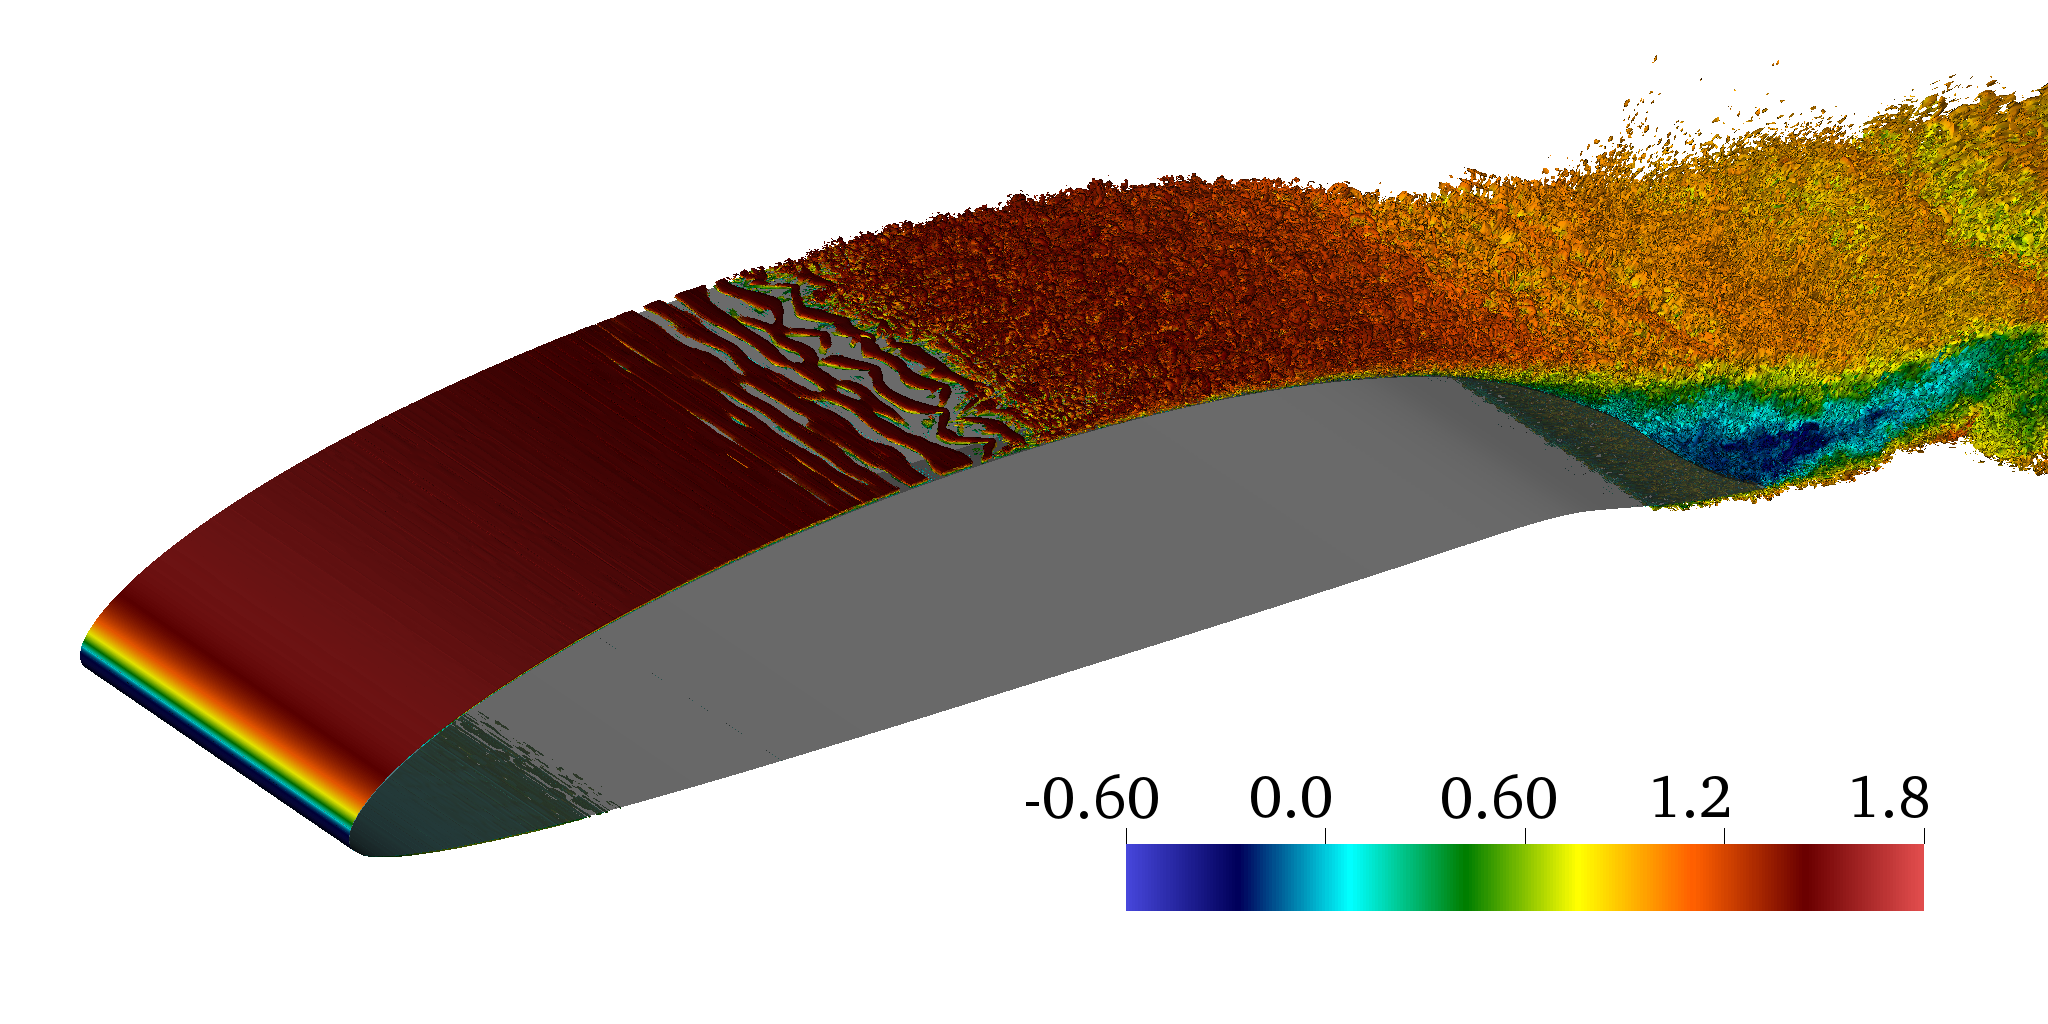
\includegraphics[width=1\textwidth]{paper2/imgs2/pitch_re750k0002}
		\label{fig:overview_la2_aoa44}		
	\end{subfigure}	
	\caption{Instantaneous vortical structures identified by the $\lambda_{2}$ criterion for the two stationary angle of attack simulations at $Re_{c}=750,000$.}
	\label{fig:overview_la2_750k_stationary}
\end{figure}

\begin{figure}[t]
	\begin{subfigure}[b]{0.49\textwidth}
		\centering
		\caption{$\alpha=6.7^{\circ}$}		
		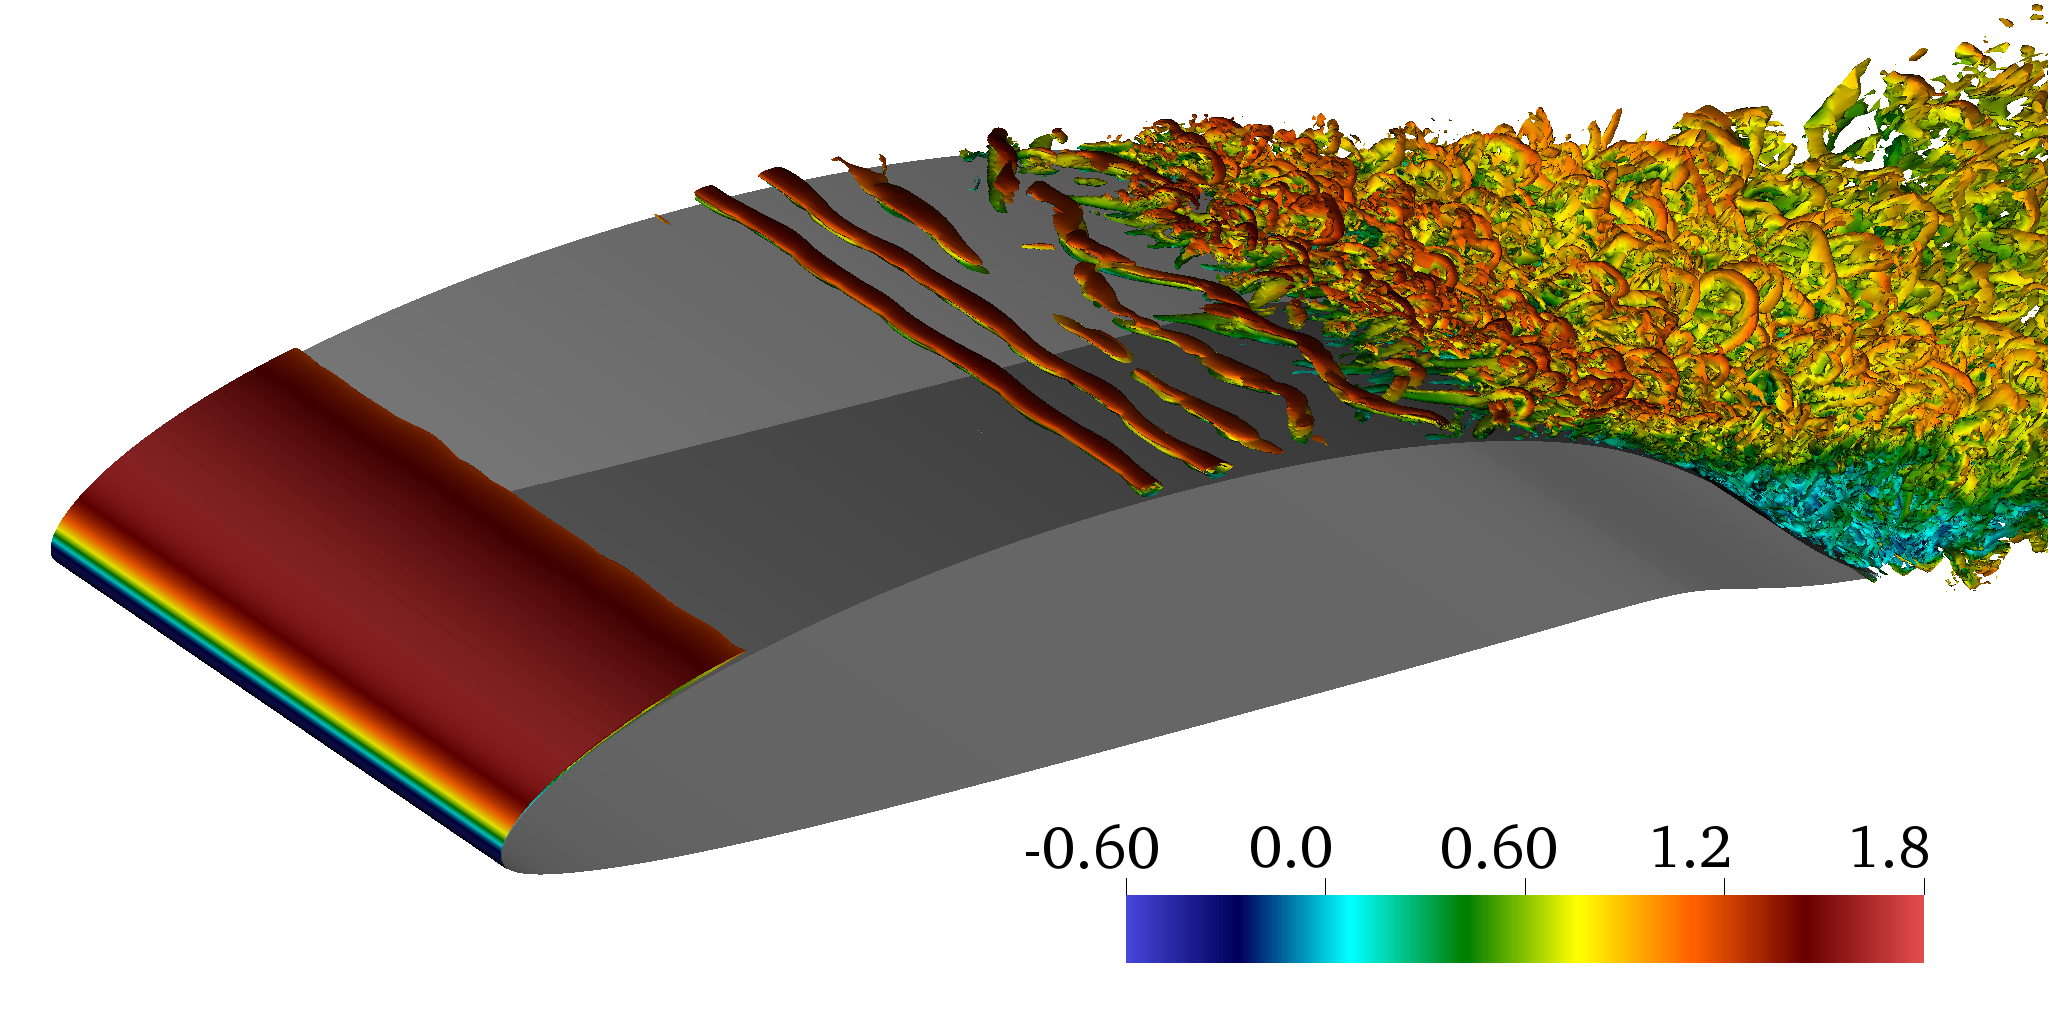
\includegraphics[width=1\textwidth]{paper3/imgs/re100k_static67_0001}
		\label{fig:overview_aoa67_iso}
	\end{subfigure}
	\begin{subfigure}[b]{0.49\textwidth}
		\centering
		\caption{$\alpha=8.0^{\circ}$}		
		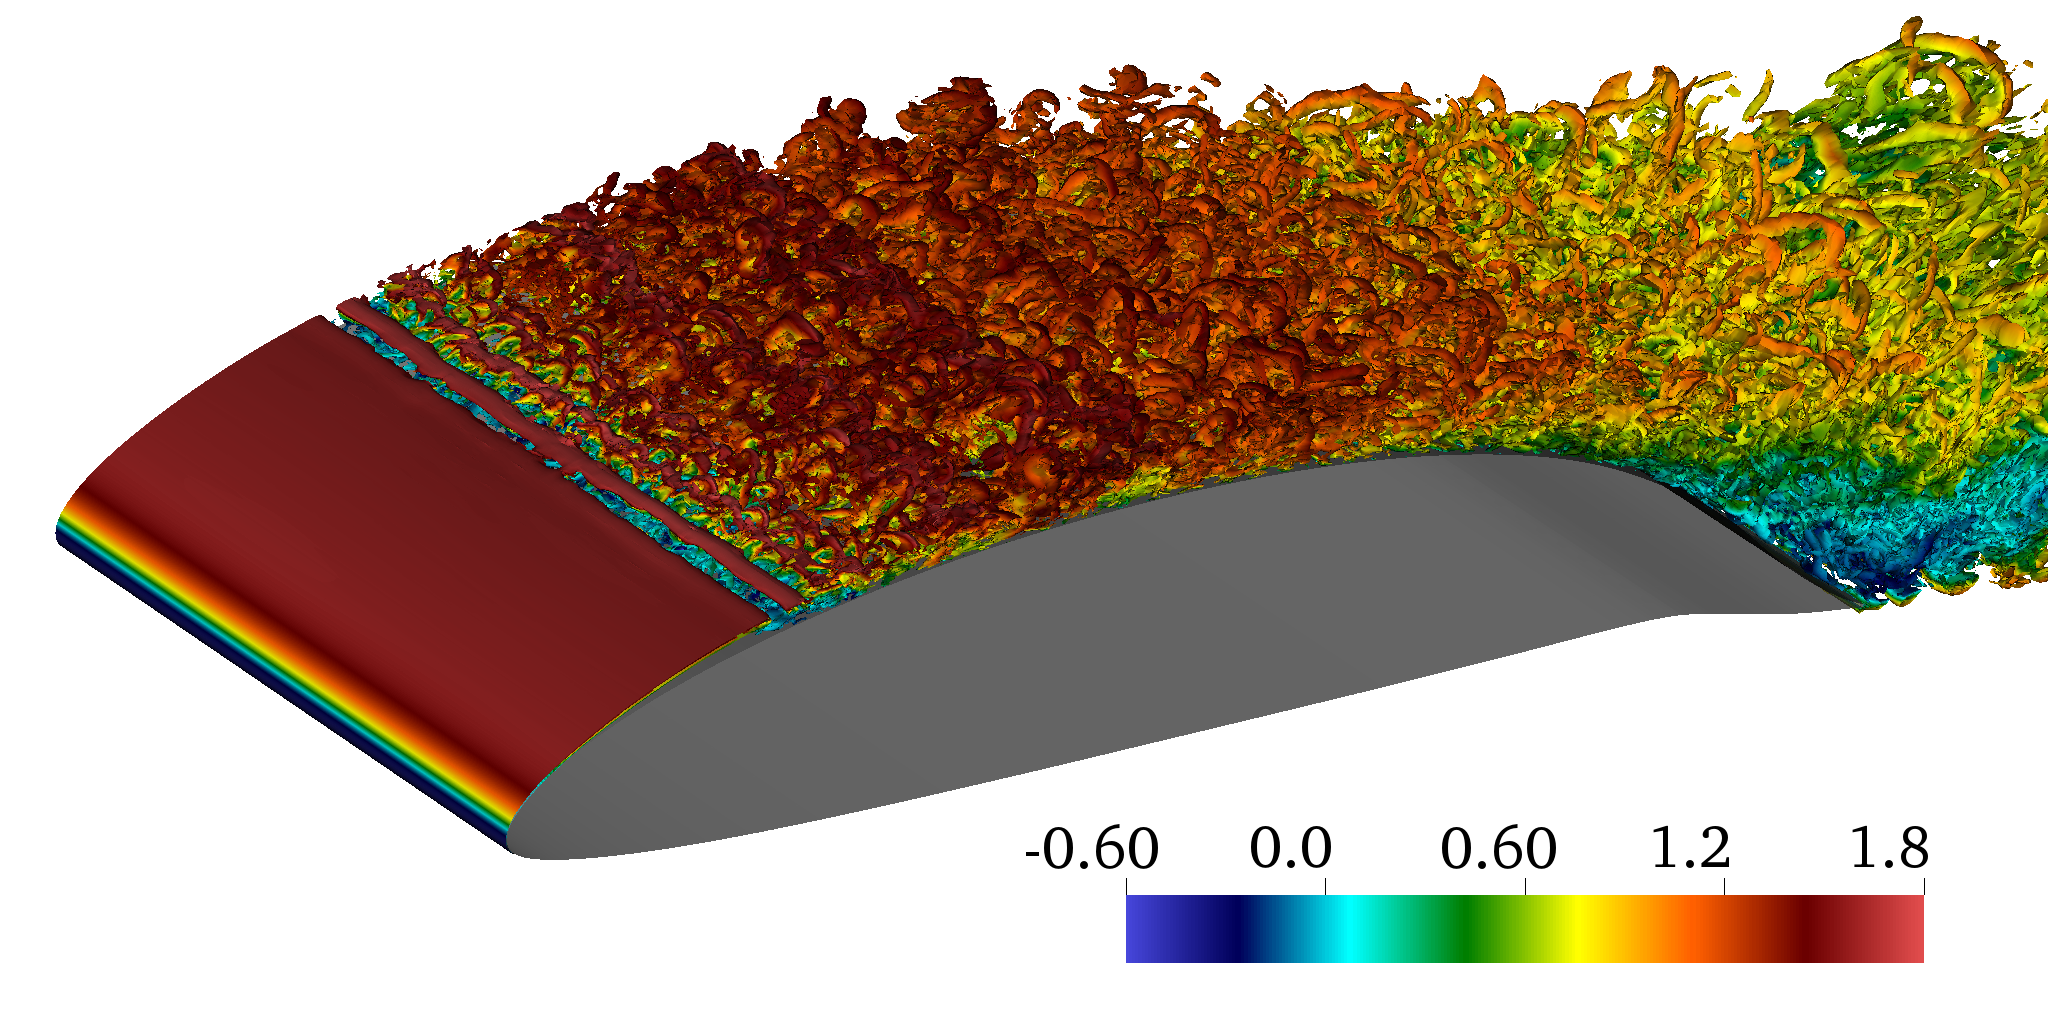
\includegraphics[width=1\textwidth]{paper3/imgs/re100k_static80_0001}
		\label{fig:overview_aoa80_iso}
	\end{subfigure}
	\caption{Isocontours of instantaneous $\lambda_{2}$ structures observed for two different (stationary) angles of attack at $Re_{c}=100,000$.}
	\label{fig:overview_isocontour_aoa}
\end{figure}

For both the Reynolds number cases, significant temporal variation of transition location is also found for the unsteady cases. Figure~\ref{fig:overview_transition_alpha} shows the variation of transition with respect to $\alpha$. The transition locations were calculated using thresholds on the instantaneous spanwise-averaged Reynolds stress $\overline{u'v'}$ and spanwise fluctuation intensity $\overline{w'w'}$. For the lower Reynolds number case the boundary layer also develops a leading-edge laminar separation bubble during the pitch cycle which significantly influences the boundary-layer dynamics.

\begin{figure}[t]
	\begin{subfigure}[b]{0.49\textwidth}
		\centering		
		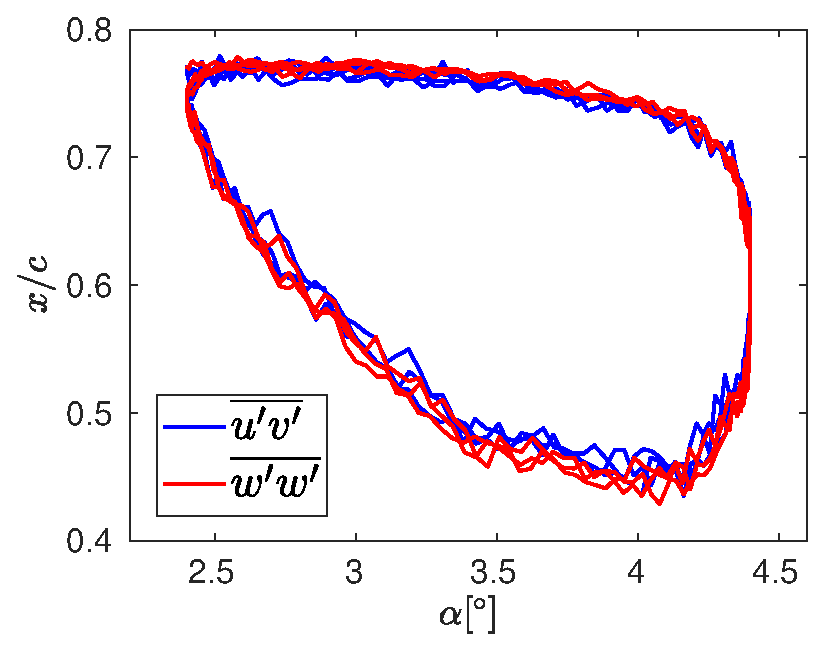
\includegraphics[width=1\textwidth,height=0.80\textwidth]{imgs/750k_transition_alpha.eps}
	\end{subfigure}
	\begin{subfigure}[b]{0.49\textwidth}
		\centering	
		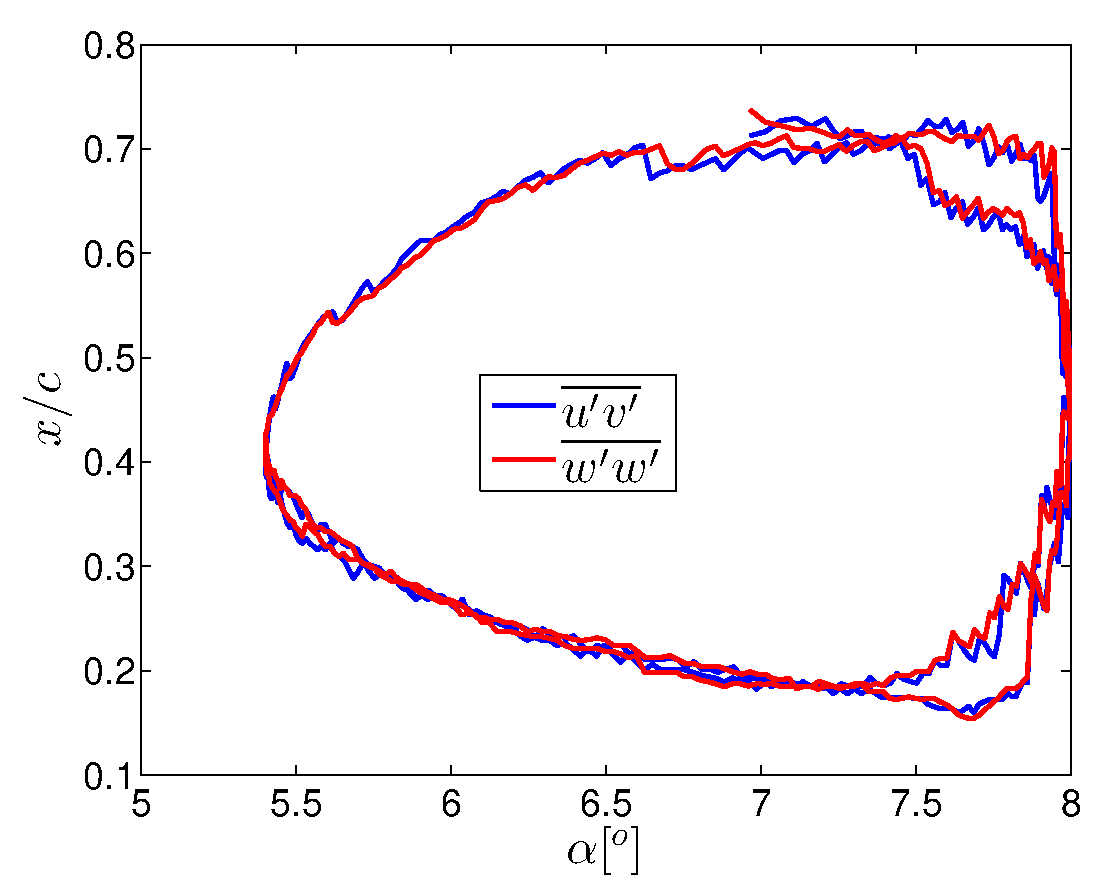
\includegraphics[width=1\textwidth]{paper3/imgs/transition_alpha.eps}
	\end{subfigure}
	\caption{Phase portraits of transition location for (left) $Re_{c}=750,000$ and (right) $Re_{c}=100,000$.}
	\label{fig:overview_transition_alpha}
\end{figure}


\section{Flow around a stationary wing section}

The final paper in the thesis deals with the study of the boundary layer over a wing section at a chord-based Reynolds number of $Re_{c}=1,000,000$. The airfoil used for the study is the asymmetric NACA 4412. A DNS database for the flow around the same airfoil at $Re_{c}=400,000$ is available and comparisons are made between the two cases to assess the effects of changing Reynolds number on the developing boundary layer. The numerical setup is done in a manner very similar to the computational study by \cite{hosseini16}. Figure~\ref{fig:overview_flow_field_re1000k} shows a section of the numerical grid and the instantaneous vortical structures in the flow field. Figure~\ref{fig:overview_beta_Reth_Ret} shows a comparison of the different measures of the boundary layer over the chord-wise distance for the two different Reynolds numbers. While both wall-shear stress (indicated by $Re_{\tau}$) and boundary layer thickness (measured with momentum thickness Reynolds number $Re_{\theta}$) change between the two cases, the Clauser parameter stays nearly the same throughout the chord. This allows comparisons across different Renolds numbers without ambiguity since the pressure gradient histories remain the same with changing Reynolds numbers. 
\begin{figure}[t]
	\centering
	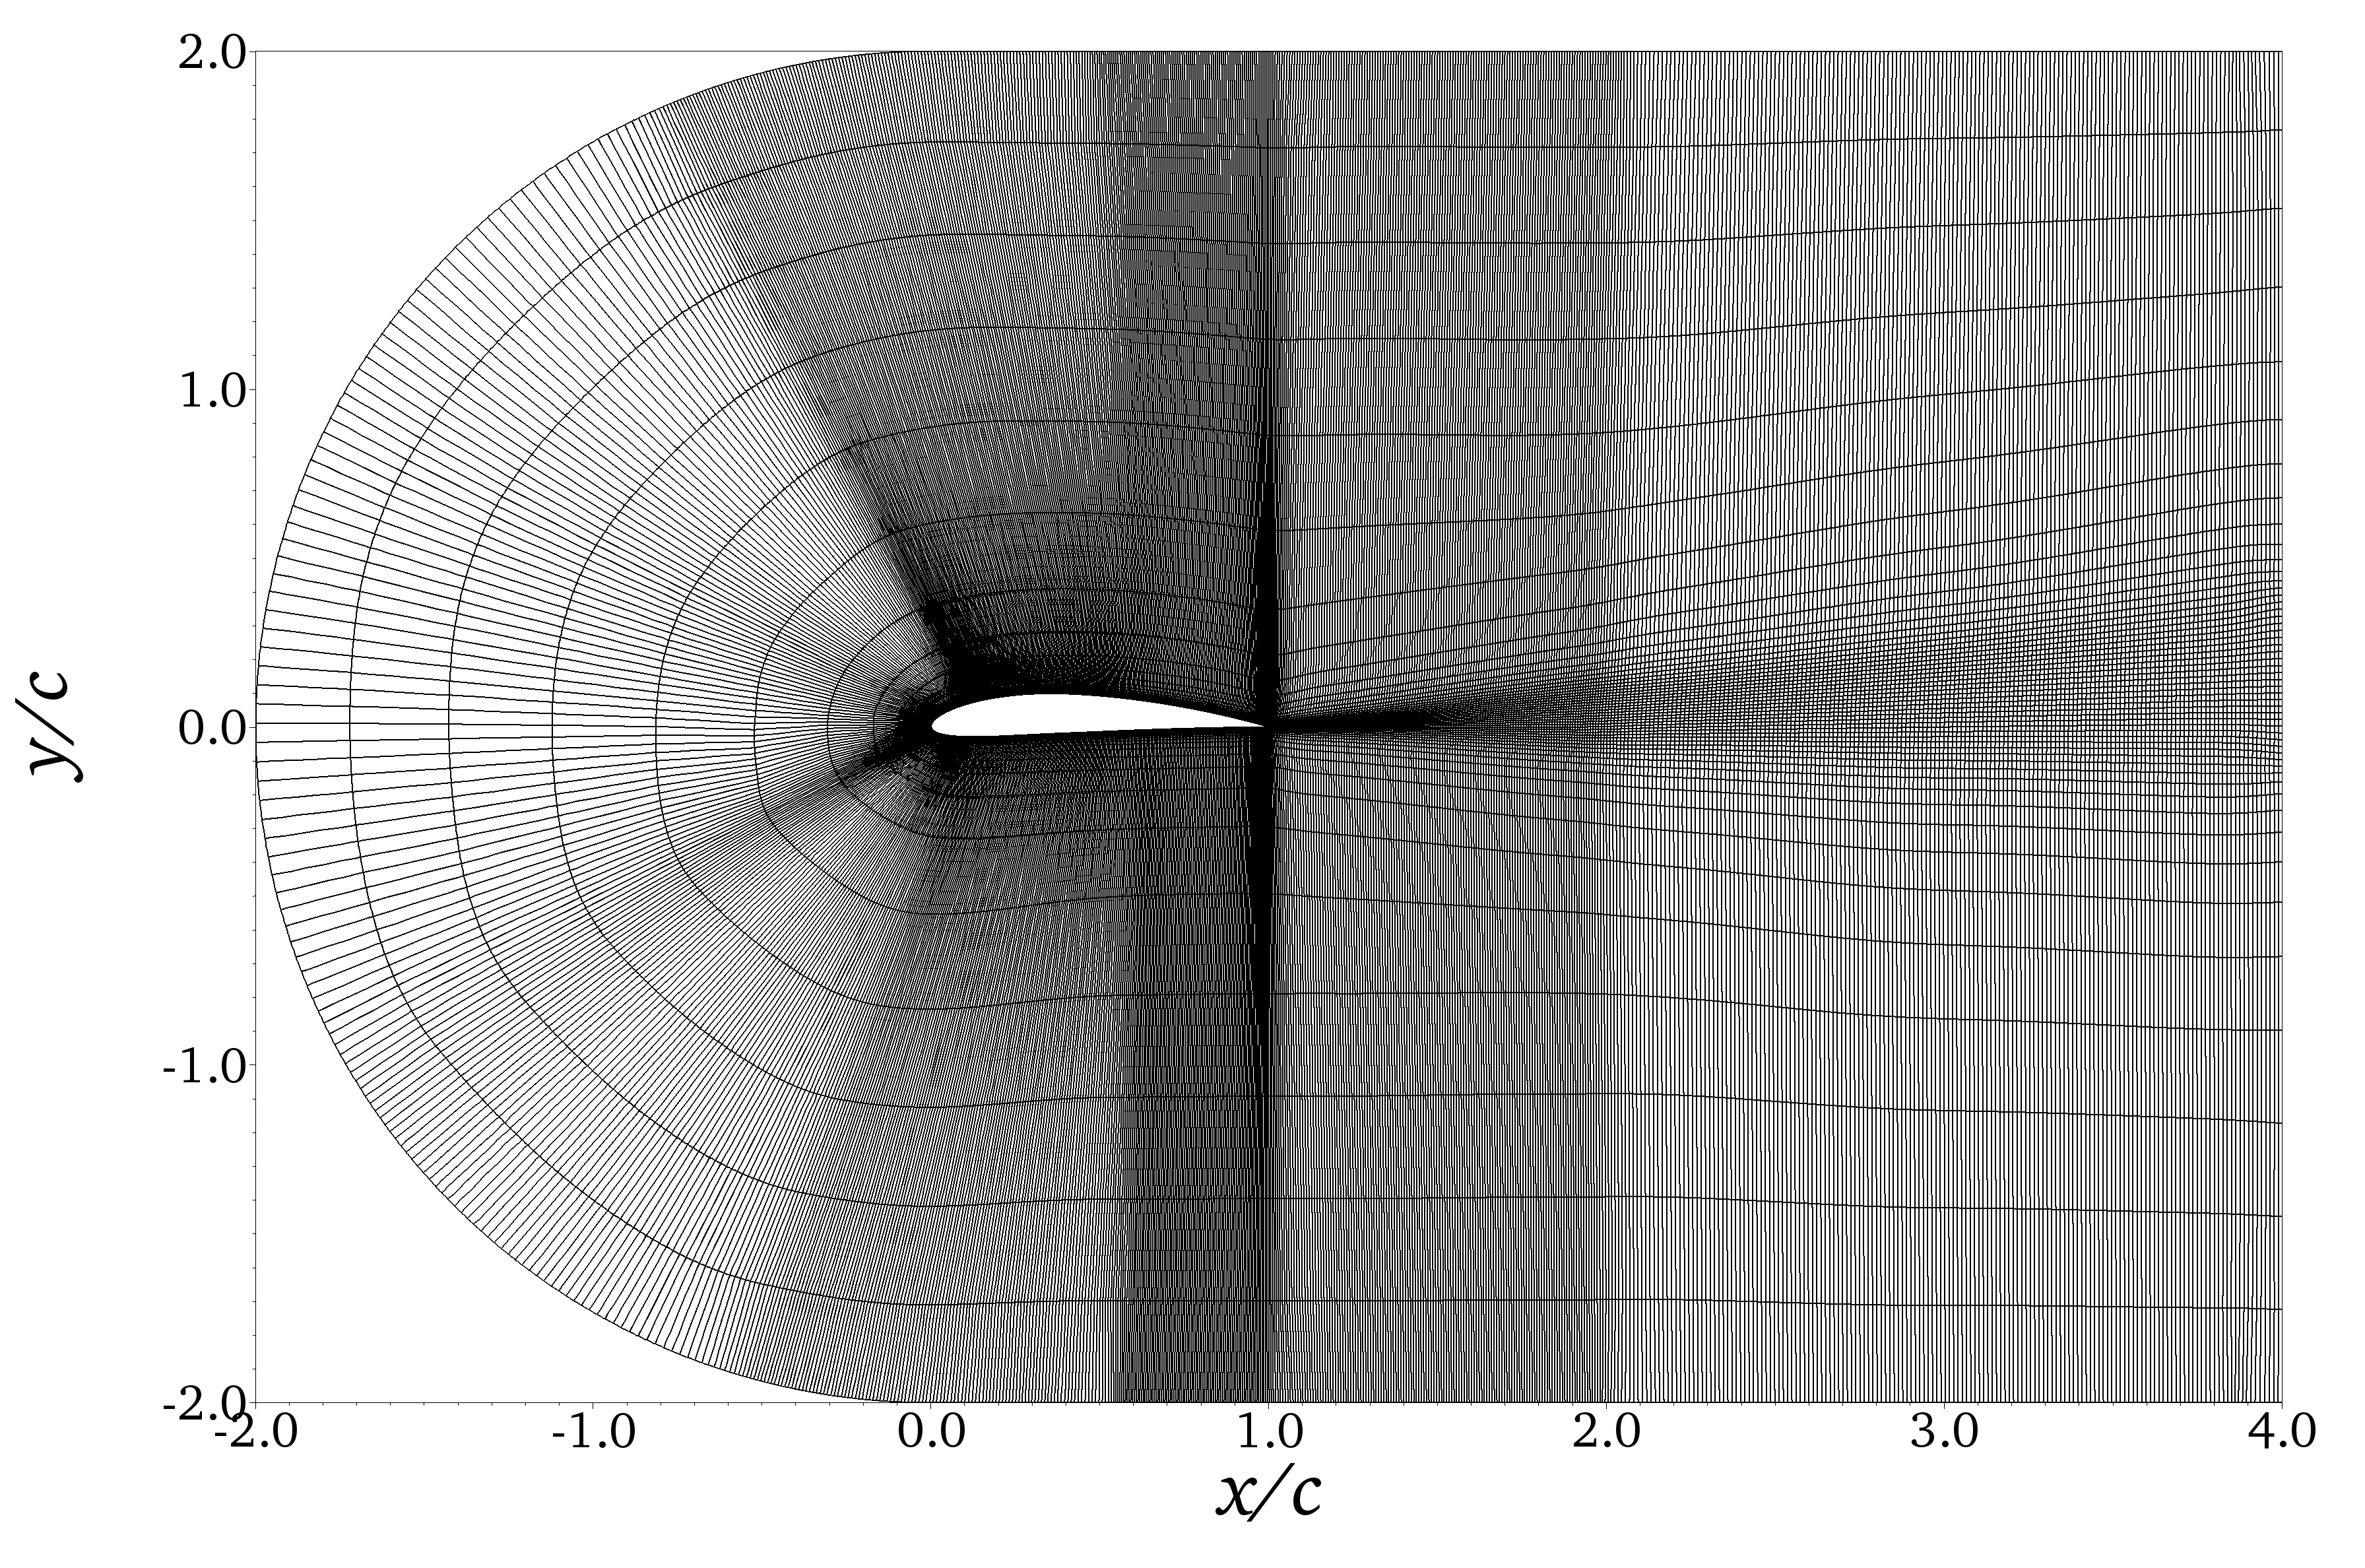
\includegraphics[width=0.49\textwidth]{paper4/imgs/wing_mesh}
	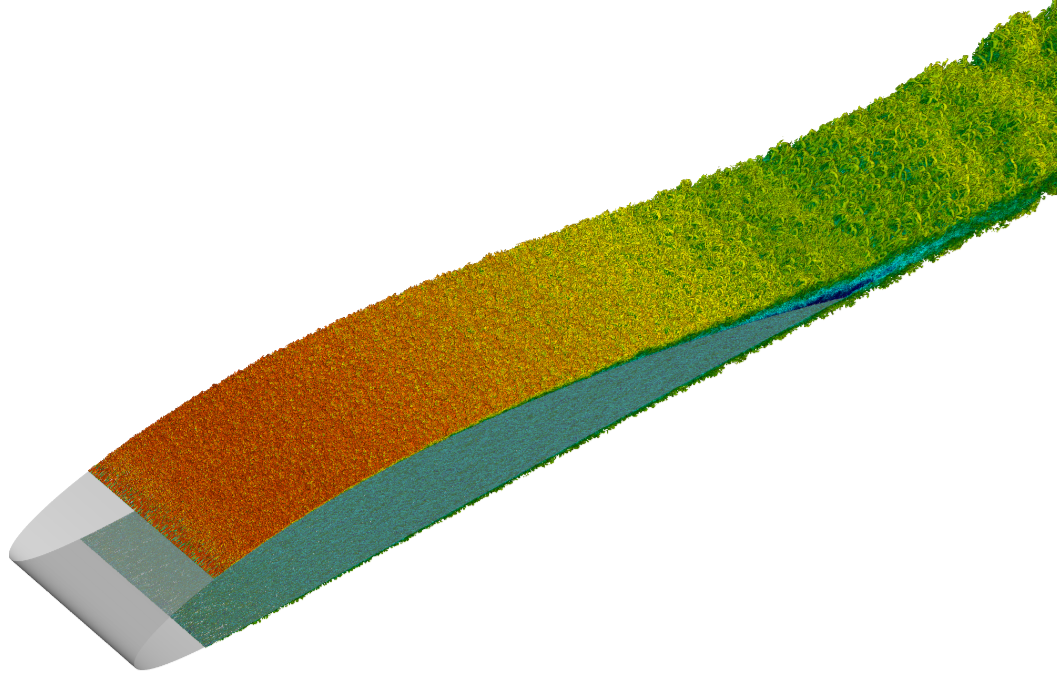
\includegraphics[width=0.49\textwidth]{paper4/imgs/wing_visualization}
	\caption{(Left) Two-dimensional slice of the computational domain showing the spectral-element distribution. (Right) Instantaneous flow field showing coherent structures identified with the $\lambda_{2}$ method \citep{jeong95}, and colored with horizontal velocity. In this figure, dark blue represents a horizontal velocity of $-0.1$ and dark red a value of $2$.}
	\label{fig:overview_flow_field_re1000k}
\end{figure}

\begin{figure}[t]
	\centering
	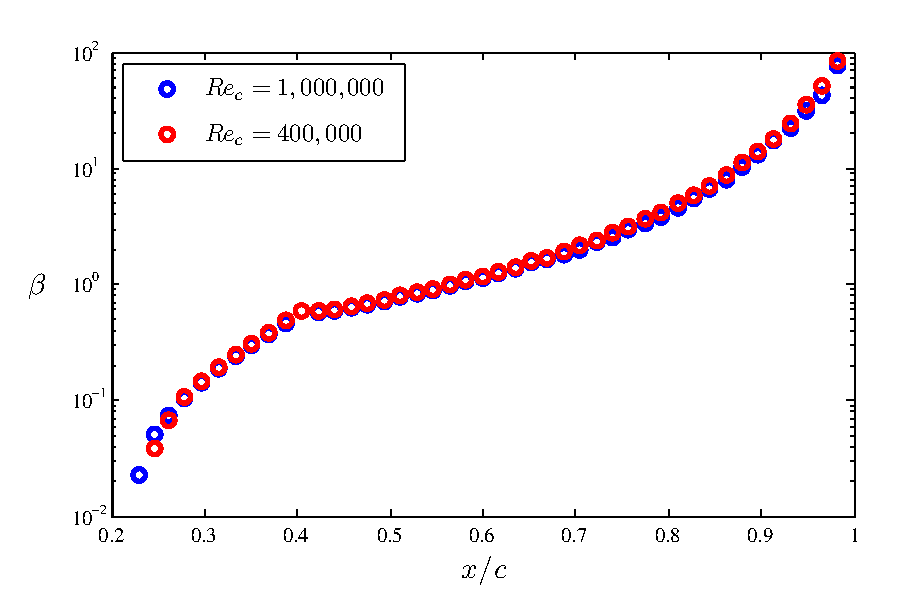
\includegraphics[width=0.49\textwidth]{paper4/imgs/beta_vs_x}
	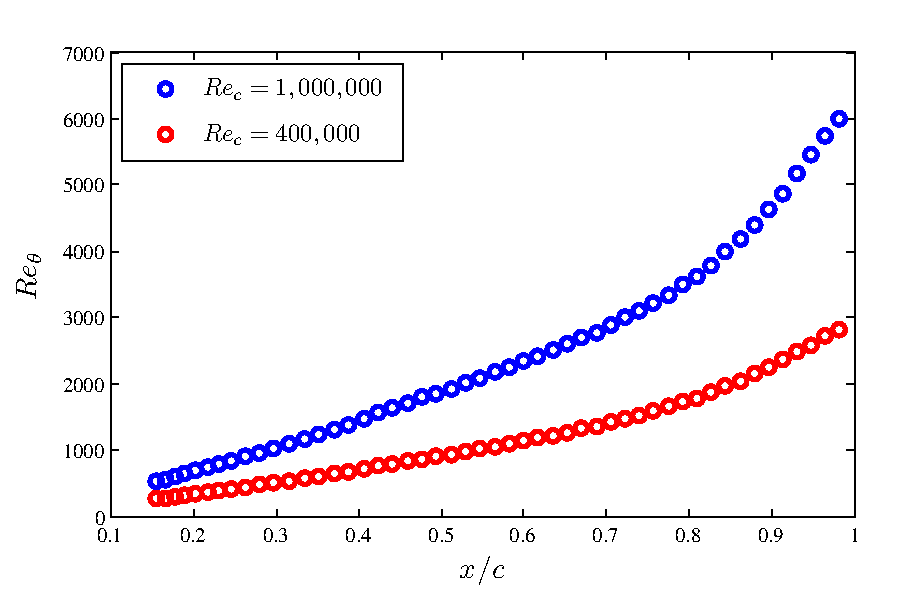
\includegraphics[width=0.49\textwidth]{paper4/imgs/Reth_vs_x}
	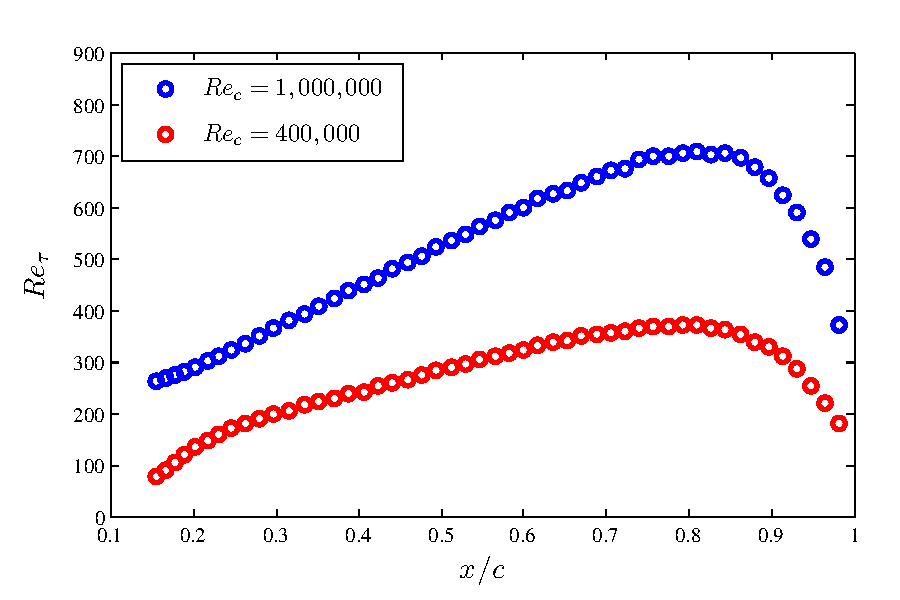
\includegraphics[width=0.49\textwidth]{paper4/imgs/Ret_vs_x}
	\caption{Streamwise evolution of (top left) the Clauser pressure-gradient parameter $\beta$, (top right) the Reynolds number based on momentum thickness $Re_{\theta}$ and (bottom) the friction Reynolds number $Re_{\tau}$, for the two wing cases under study.}
	\label{fig:overview_beta_Reth_Ret}
\end{figure}

%===============================================================================
\chapter{Conclusions and outlook}
%===============================================================================

The current thesis work concerns three different fields of research.

In the first part of the thesis, the ``evolve and filter'' technique for the stabilization of spectral-element methods is analyzed and it is found the filter operation causes an undesirable loss of divergence-free quality of the solution. This loss of divergence is shown to be particularly large for the test case of a double shear layer. An alternate formulation of the stabilization called the relaxation-term (RT) stabilization is shown to overcome the drawbacks of the explicit filtering technique, while maintaining the simplicity of the original explicit filter. This RT stabilization technique is very closely related to explicit filtering, with the two operations being equivalent to the leading order in time. Stability limits of the RT stabilization are explored and is shown to be stable within the practical parameter range.

In the second part, an NLF airfoil undergoing small-amplitude pitch-oscillations is analyzed at two different Reynolds numbers. In both cases a large variation of transition, and thus boundary layer characteristics is observed over the airfoil resulting in a non-linear response of the aerodynamic force coefficients. For $Re_{c}=750,000$ it shown that the temporal evolution of the transition point can be understood with a simple phase-lag concept, with the implication that boundary-layer evolution may be considered quasi-steady in time. Using this phase-lag concept a simple empirical model is developed which is able to explain a fairly wide range of experimental data.

On the other hand, for $Re_{c}=100,000$ a qualitatively different picture emerges for the unsteady boundary layer. The boundary-layer response displays a dynamically rich behavior with marked asymmetry of upstream and downstream transition movement. In this case, transition location is governed by the properties of the leading-edge laminar separation bubble (LSB) and it is conjectured that the absolute instability of the LSB may be responsible for abrupt changes in boundary layer characteristics.

Finally, in the third part of the study, flow over a stationary NACA 4412 airfoil is studied at two different Reynolds numbers with the aim of better understanding the boundary-layer evolution in non-equilibrium pressure gradient boundary layers. Two flow cases at a chord-based Reynolds number of $Re_{c}=400,000$ and $Re_{c}=1,000,000$ are compared at different streamwise locations. It is found that the effect of the streamwise pressure gradients is higher at low Reynolds numbers, leading to greater energy in the larger structures present in the outer part of the turbulent boundary layer.

The current work has laid the foundation for several interesting questions that may be the focus of future work. Can the simple empirical aerodynamic model be extended for a wider range of unsteady motions? Can the phase-lag be predicted a-priori as in the case of the classical model by \cite{theodorsen35}? When does the quasi-steady assumption break down and the boundary layer becomes truly unsteady? For $Re_{c}=100,000$, can the asymmetry of the (upstream and downstream) velocities of transition point be linked with the stability properties of the LSB? What is the influence of free-stream turbulence on unsteady LSB? In stationary airfoils, how does the velocity spectrum change with Reynolds number in non-equilibrium flows? What are the characteristics of boundary layer streaks in non-equilibrium flows? Some of these questions will be the focus of further research.


%===============================================================================
% Acknowledgments
%===============================================================================
%


\begin{acknowledgements}
	My foremost gratitude goes to my supervisor Dan Henningson for giving me the opportunity to join his research group. His knowledge and guidance have helped me immensely as a student. His encouragement, for which there is no substitute, have always provided the inspiration I needed to constantly push myself further in my work. Next I would like to thank my co-advisors Philipp Schlatter and Ardeshir Hanifi. Philipp for his patience during all my ignorant and sometimes foolish questions on numerics, conferences, papers and others that I probably can't recall. Ardeshir for the laughter, the sandwiches, the beers and most importantly, always being available on short notice when I needed help. I would also like to thank the members of the NFFP project, Roger Larsson, Dr. David Eller and Dr. Mikaela Lokatt for all the interesting discussions on aerodynamics. 
	
	I am grateful to Adam Peplinski for all the help he provided with Nek5000, MPI and coding in general. I can not imagine figuring out the workings of Nek5000 without his support. Armin and Ricardo have helped me more than others during my crucial time as a new Phd student. The help is greatly appreciated.
	
	Special mentions go to Mattias for all the coffee breaks, introducing me to Swedish food, the spontaneous discussions and being the bouncing board for all my (mostly wrong) ideas. Your company shall be missed once you leave the department. Jacopo and Giandomenico for all the great company, joining for the spontaneous plans and granting me the honorary Italian citizenship. I'll learn Italian very soon I promise! Marco for the constant dinner company. Freddy for the weekend food+beer+movie routine. Elektra for being one of the greatest friends of all time. Politics, late-night and of course Trump shall keep us entertained for times to come. But mostly, thanks for correcting my manuscripts and the support during this licentiate period. A mention must also go to my unrequited love, Walter Fornari. Where will I find another like you?
	
	A hearty thanks goes out to all my friends here at the department who make this a wonderful place. Eric, Clio, Nicolas, Sudhakar, Ugis, Evelyn, Anthony, Mehdi, Ali, Guillaume, Luca, Luca, Pierluigi, enrico, Francesco, Kristina, Ekatrina, J.C., Matthias, Priti, Ninge, Sagar, Krishne, Dhiya, and everyone else. All of you, with your quirks, jokes, stories and gossip (looking at you Pierluigi) add a little bit of color to life everyday.
	
	Perhaps most importantly, my deepest gratitude goes towards my family for their patience, unconditional love and support during my ever wandering path through life.
	
	Lastly, financial support for this work was provided by Vinnova through the NFFP project UMTAPS, with grant number 2014-00933, the Knut and Alice Wallenberg Foundation, and the European Research Council under grant agreement 694452-TRANSEP-ERC-2015-AdG.\ The computations were performed on resources provided by the Swedish National Infrastructure for Computing (SNIC) at the PDC Center for High Performance Computing at the Royal Institute of Technology (KTH). Simulation have also been performed at the Barcelona Supercomputing Center, Barcelona, with computer time provided by the $12^{th}$ PRACE Project Access Call (number 2015133182) and at the High Performance Computing Center, Stuttgart (HLRS) with the computer time provided by the $15^{th}$ PRACE Project Access Call (number 2016163965). 

\end{acknowledgements}



%===============================================================================
% References
%===============================================================================
%
\bibliographystyle{jfm}
\bibliography{licentiate}
%
\IfFileExists{overview.bbl}{\graphicspath{{imgs/}}
%\setlength{\captionmargin}{50pt}

%===============================================================================
\chapter{Introduction}
%===============================================================================
\section{A short history}

The first sustained flight by the Wright brothers in 1903 marked a historic day in human achievement and ingenuity. Momentous as the achievement was, the Wright brothers did not truly invent the modern airplane. Their achievements were the fruition of nearly a century of aeronautical research, starting perhaps with Sir George Cayley, who is considered the ``father of aerial navigation'' \citep{gibbs-smith62}. The principal components of the modern aircraft were laid down by George Cayley as early as 1799. Prior to Cayley, the ideas for mechanical flight tended towards flapping wings, where the flapping motion produced both propulsion and lift. George Cayley was the first to break the unsuccessful chain of thought and separated the two aspects of flight into distinct systems. His triple paper ``On Aerial Navigation'' published in Nicholason's \textit{Journal of Natural Philosophy, Chemistry and the Arts} on November 1809, February and March 1810 \citep{cayley1809} mark some of the most important works in aeronautical history. In the works, Cayley states for the first time, the principle of lift generation \textit{i.e.} the formation of a low pressure region on the upper surface of the wing. His paper elaborates on the separation of lift from propulsion and also goes on to talk about flight control and airplane stability. Later in his life, he proposed the concept of multiplanes (multiple wings mounted on top of each other) and built the first glider triplane named the ``boy carrier'' in 1849.

Several investigators followed the quest of ``aerial navigation''. Otto Lilienthal was the first to design and successfully fly controlled gliders in 1891, going on to make over $2500$ successful glider flights. Octave Chanute brought aeronautics research to America and designed a biplane glider which directly inspired the designs of the Wright Brothers. Samuel Pierpont Langley was a contemporary of the Wright brothers who built and tested several powered model airplanes. His success in achieving powered flight directly influenced and encouraged the Wright brothers. The final historic achievement of successful powered flight was achieved by the Wright brothers. On December $17^{th}$ 1903, a gasoline powered biplane by the name Wright Flyer I (figure~\ref{fig:wright_flight}) took flight in (modern day) Kill Devil Hills, North Carolina, ushering forth the era of practical human flight.
\begin{figure}[h]
	\centering
	\includegraphics[width=0.90\textwidth]{wright_brothers_first_flight}
	\vspace{10pt}	
	\caption{First flight of the Wright Flyer I, December 17, 1903, Orville piloting, Wilbur running at wingtip. Image from \cite{wikipedia_wright}.}
	\label{fig:wright_flight}
\end{figure}

\section{Modern aircraft design}
Since that fateful day, modern airplanes have been used in a variety of different conditions, varying from commercial passenger planes, to supersonic military aircrafts \citep{blackbird}, 
to endurance flights around the world lasting 9 days \citep{rutan_voyager}. The myriad uses have resulted in various challenges that need to be overcome by the aircraft designers. One significant challenge has been due to the dynamic interaction of air flow with the airplane structures, now studied under the field of aeroelasticity. These problems came to the fore as the design speed of aircrafts increased over the years and designers came to favor monoplanes over the biplane design. An early example was that of the Fokker D-8 German aircraft during World War I which suffered wing failure under steep dives, which was the first documented case of static aeroelastic effects.

Today the designers of commercial aircrafts face another challenge brought about by global climate change and rising oil prices. With the realization of the contribution of the aviation industry towards global climate change \citep{green08}, aircraft designers now face a need to significantly improve the fuel efficiency of commercial aircrafts in a bid to reduce the carbon footprint of the industry. In an effort to quantify the opportunities of achieving such an improvement, \cite{schrauf05} showed a break-down of the drag experienced by a typical transport aircraft highlighting that frictional drag accounted for more than half the drag experienced by the aircraft. Clearly a favorable modulation of the boundary layer over the wing could help achieve large improvements in fuel efficiency. The modulation could come in the form of effective flow control strategies, or with wing design strategies such as the use of natural laminar flow (NLF) airfoils. Both \cite{schrauf05} and \cite{green08} push forward the idea that NLF airfoils and laminar flow control strategies are the low-hanging fruits in the goal of higher fuel efficiency and a concerted effort into addressing the engineering challenges for practical implementation must be made. Some of these challenges may require revisiting the aeroelasticity problems from the perspective of laminar wings. However laminar flow at high Reynolds numbers is susceptible to destabilization and may not always be possible. Thus turbulent drag reduction strategies need to be used effectively where needed \citep{bushnell03}. Whatever the form of drag reduction technique that may finally be implemented on a particular aircraft, the understanding of developing boundary layers over wings (including the influence of control strategies) occupies a central position in aerodynamic research if the goal of higher fuel efficiency is to be realized. With this goal in mind, the current thesis work aims to further the understanding of developing boundary layers over airplane wings, focusing on two particular aspects.
\begin{itemize}
	\item Understanding the structure of the turbulent boundary layer developing over a wing section.	
	\item Understanding the evolution of the developing boundary layer over a natural laminar flow airfoil in unsteady flight conditions. 
\end{itemize}

%Solutions to these emerging aeroelastic problems needed an understanding of the unsteady phenomenon occurring in practical flight conditions. Such understanding came via the works of \cite{glauert30,karman38,theodorsen35} \textit{etc}, and by the 1940s, design engineers had the tools to account for unsteady aeroelastic effects in their wing designs.

%The achievements of these early aerdynamicists is quite impressive in particular considering that the boundary layer concept was in its nascent stages when the first practical airplanes were being designed. Indeed Prandtl's revolutionary concept of a boundary layer was first presented in 1904, almost a full year after the first flight of the Wright brothers.  

%-------------------------------------------------------------------------------
\section{Boundary layers over a stationary wing}

The understanding of the structure and scaling of wall-bounded turbulent flows has been in study for several decades and a complete understanding still remains far from complete. These flows have been studied with different canonical geometries such as channels \citep{kim87,moser99,lee15}, pipes \citep{elkhoury13,jimenez08,chin15} and flat plates \cite{spalart88,schlatter10,eitel14}. For the case of spatially evolving boundary layers over a flat plate, the simplest canonical case involves boundary-layer evolution subjected to a zero pressure gradient (ZPG). These flows may be uniquely characterized by a single parameter, \textit{i.e.} the Reynolds number Re, which is the ratio of the inertial and viscous scales of the flow. However practical flow cases are often influenced by pressure gradients. Such flow cases can no longer be uniquely defined using a single parameter. \cite{clauser54} with intuitive reasoning proposed a concept of an equilibrium boundary layer which may be uniquely defined by two parameters. He argued that, if the ratio of the average pressure gradient force across the boundary layer and the viscous shear force at the wall remains constant, the boundary layer would experience a similar flow history throughout its evolution. Thus the equilibrium pressure gradient boundary layers are uniquely defined by two parameters, namely the Reynolds number (Re) and the pressure gradient parameter $\beta$, defined as
\begin{eqnarray}
	\beta = \delta^{*}(dp/dx)/\tau_{w},
\end{eqnarray}
where $\delta^{*}$ is the displacement thickness, $dp/dx$ is the pressure gradient and $\tau_{w}$ is the wall-shear stress. The parameter is commonly referred to as the Clauser parameter. A flow case with a spatially constant Clauser parameter is categorized as an equilibrium boundary layer and a ZPG boundary layer is a special case of an equilibrium boundary layer with $\beta=0$. Several works have focused on pressure gradient boundary layers ranging from theoretical studies by \cite{townsend56,townsend56b,mellor66}, experimental works of \cite{skare94,harun13} and numerical simulations by \cite{spalart93,skote98}. The developing boundary layer over an airfoil however further increases in complexity since these boundary layers fall under the category of non-equilibrium boundary layers where the Clauser parameter is spatially varying. In such cases the flow history also plays a role in determining the local boundary layer properties \citep{clauser54,bobke17}. Analysis of such flow cases becomes significantly more difficult since the local boundary layer parameters do not uniquely define the state of the boundary layer. Nonetheless the study of such boundary layers is important since generic boundary layers found in nature would belong to this category, including the boundary layers over wings. The boundary layer developing over the NACA 4412 airfoil has the property that the spatially varying Clauser parameter is insensitive to Reynolds number. The presents us with the opportunity to study the Reynolds number effects of a non-equilibrium boundary layer with a constant pressure gradient history. That is indeed the methodology followed in this work. The developing boundary layer over a NACA 4412 wing section is analyzed at two different Reynolds numbers in order to understand Reynolds number effects in non-equilibrium boundary layers.

\section{Unsteady boundary layers}
%
Unsteady aeroydnamic studies started with the emergence of aeroelastic phenomenon in the early part of the $20^{th}$ century. With the gradual shift to monoplane designs, the inherent high torsional stiffness of biplanes was lost and aerodynamic instabilities, such as the one experienced by the Fokker D-8 became important. Pioneering works of \cite{glauert30,karman38,theodorsen35} \textit{etc}, provided the insight and modeling of such unsteady aerodynamic behavior and by the 1940s the foundations of unsteady aerodynamics for incompressible attached flows had been laid down. The mathematical framework these unsteady aerodynamic theories relied on simple inviscid and quasi-steady assumptions, which proved to be highly attractive to the wing designers \citep{leishman00}. Experimental corroboration by \cite{halfman52} and \cite{rainey57} further added support to the validity of the simple assumptions. Over the next few decades, investigations of unsteady aerodynamics shifted focus to the understanding of the dynamic stall phenomenon, with works of \cite{mccroskey76,mccroskey81,mccroskey82experimental,mccroskey82,carr1977,crisler94}. A large body of work on unsteady separated flows was presented by \cite{ericsson86,ericsson87b,ericsson_stall88a,ericsson_stall88b}. The studies continue to this day with the works of \cite{visbal11,visbal14,visbal17,dunne2015} and several other authors, a recent review can be found in \cite{coorke15}. 
\begin{figure}[h]
	\centering
	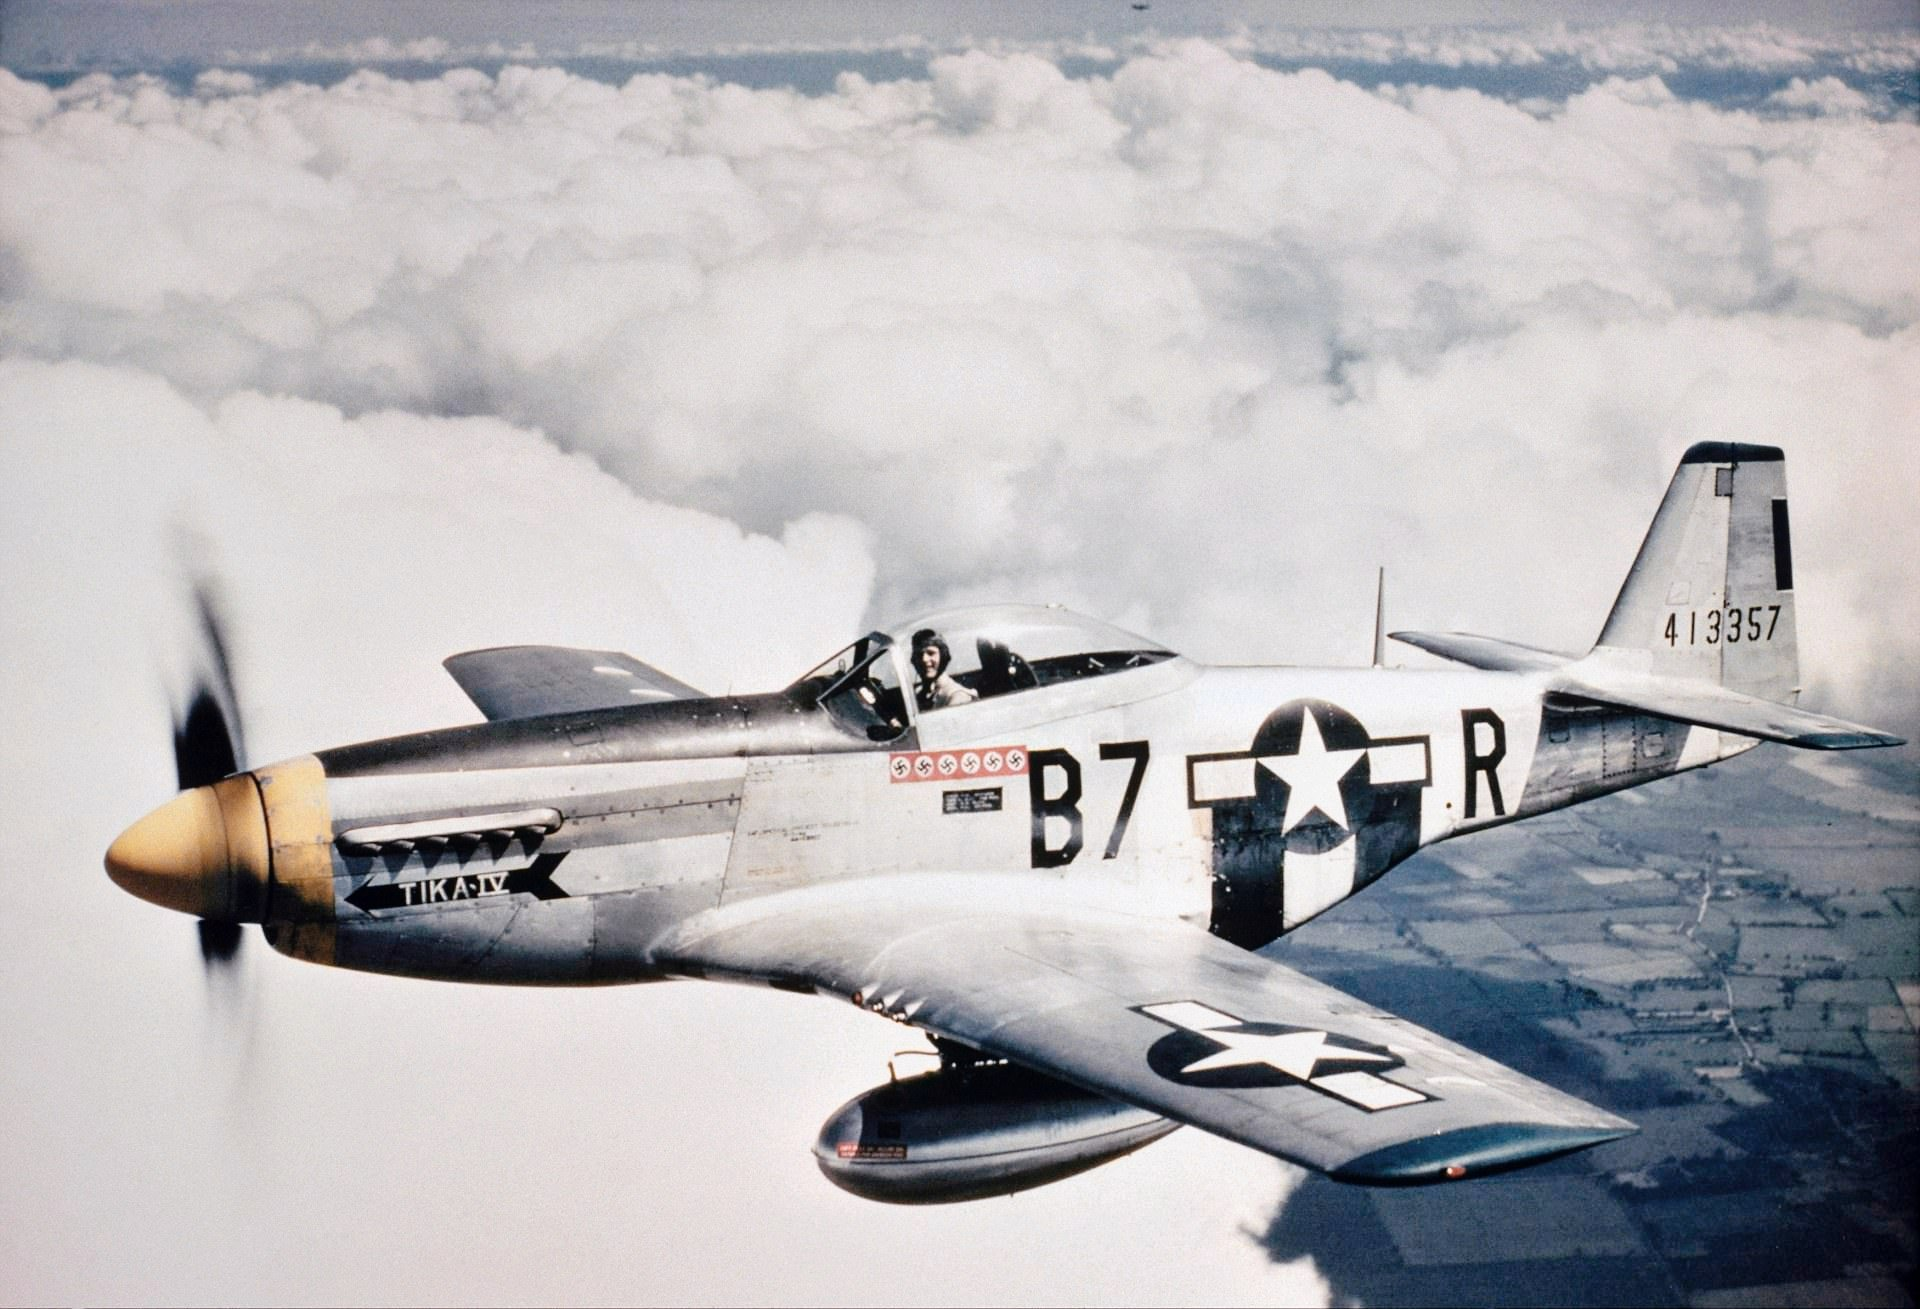
\includegraphics[width=0.90\textwidth]{P-51-mustang}
	\vspace{10pt}
	\caption{North American P-51 Mustang. Image from \cite{wikipedia_mustang}.}
	\label{fig:mustang}
\end{figure}

However it appears that the aeroelasticity problem was not considered from the perspective of natural laminar flow airfoils. This is a surprising fact considering the P-51 Mustang (figure~\ref{fig:mustang}), a fighter aircraft in the Royal Air Force designed in 1940, incorporated a wing with a natural laminar flow airfoil section \citep{green08}. The first aeroelastic study on laminar wings was performed as late as 2011 by \cite{mai11}. This, along with a subsequent investigation by \cite{hebler13}, brought to light a peculiar characteristic of unsteady laminar wings, \textit{i.e.} the presence of non-linearities in the unsteady aerodynamic forces. The classical unsteady aerodynamic theories did not predict non-linear unsteady responses and thus fail to account for such behavior. Inspired by this, \cite{lokattthesis} performed experiments on unsteady NLF airfoils and also found strong non-linearities in the aerodynamic forces. Consistent in the explanation for the non-linearities in all these studies was the role of transition over the wing surface. When transition on the airfoil suction-side was fixed (with a trip) near the leading edge, the non-linearities seemed to disappear. These results indicated a need for a more in-depth study of the evolving boundary layer in such unsteady laminar airfoils. Classical theories negate the role of the boundary layer by invoking the inviscid assumption and it is apparent that such an assumption is no longer be justified for laminar wings. Characteristics of the unsteady boundary layer are the subject of investigation in the present work.

\thesisstructure The thesis is structured as follows:
\begin{itemize}
	\item An overview of the numerical method used for the simulations is given in Chapter 2.
	\item Chapter 3 gives an overview of the numerical simulations performed in the study.
	\item The main conclusions of the current work are given in Chapter 4 along with an outlook for future work.
	\item The next part of the thesis includes the individual papers and internal reports. 
\end{itemize}

%===============================================================================
\chapter{Numerical Method}
%===============================================================================

\section{Numerical Discretization}

The numerical code used for the simulations is Nek5000, which is an open source research code developed by \cite{nek5000} at Argonne National Laboratory. The code solves the incompressible Navier--Stokes equations (\ref{eqn:navier_stokes}) in non-dimensional form:
\begin{subequations}
	\label{eqn:navier_stokes}	
	\begin{eqnarray}
	\frac{\partial u_{i}}{\partial t} + u_{j}\frac{\partial u_{i}}{\partial x_{j}} =  - \frac{1}{\rho}\frac{\partial p}{\partial x_{i}} + \frac{1}{Re}\bigg(\frac{\partial^{2} u_{i}}{\partial x_{j}\partial x_{j}}  \bigg) +f_{i} \\
	\frac{\partial u_{i}}{\partial x_{i}} = 0
	\end{eqnarray}
\end{subequations}
where $x_{i}$ is the coordinate direction, $u_{i}$ is the velocity component, $p$ is the pressure and $Re$ is the defined Reynolds number. The discretization of the Navier--Stokes equations is based on a spectral-element method, first proposed by \cite{patera84}. The method allows the mapping of elements to complex geometries along with a high-order spatial discretization within the elements, thus combining the generality of finite-element methods with the accuracy of spectral methods \citep{patera84}.
The spatial discretization in each element is performed following the $P_{N}$-$P_{N-2}$ \citep{maday89} formulation with velocity represented by high-order Lagrange interpolants through the Gauss--Lobatto--Legendre (GLL) quadrature points, while the pressure is represented on the staggered Gauss-Legendre (GL) quadrature points. The nonlinear terms are treated explicitly by third-order extrapolation (EXT3), while the viscous terms are treated implicitly by a third-order backward differentiation scheme (BDF3). Over-integration is used for the removal of aliasing errors. Nek5000 is written in Fortran 77 and C with efficient scaling for up to 1 million MPI ranks \citep{fischer15}.

%%%%%%%%%%%%%%%%%%%%%%%%%%%%%%%%%%%%%%%%%%%%%%%%%%%%%%%%%%%%%%%%%%%%%%
\section{Relaxation-term large-eddy simulation (RT-LES)}

Owing to the high Reynolds numbers and large time-scales of integration for some of the flow cases, a direct numerical simulation (DNS), which requires a resolution of all the spatial scales of the flow, leads to prohibitively high computational costs. In recent years a technique of wall-resolved large-eddy simulations has emerged as a computationally cheaper alternative to DNS, while also exhibiting the high-fidelity characteristics of DNS.
The technique has been utilized in the studies of spatially developing boundary layers \citep{eitel14}, pipe flows \citep{chin15} and flow over wings \citep{uzun10,lombard15}. The success of the approach has motivated its use in the present work. The wall-resolved LES method used is based on the RT3D variant of the ADM-RT approach first used by \cite{schlatter04}. The method has been shown to be reliable in accurately predicting transition and also preserving the characteristic structures which are seen in the DNS of transitional flows by \cite{schlatter06}. This particular quality of the LES model is crucial since there is a large focus on the unsteady transition in the present work. The LES method supplements the governing equations with a dissipative term $-\chi\mathcal{H}(u)$. The equations of motion for the resolved velocity and pressure thus read as
\begin{subequations}
	\label{eqn:rt_les}	
	\begin{eqnarray}
	\frac{\partial u_{i}}{\partial t} + u_{j}\frac{\partial u_{i}}{\partial x_{j}} =  - \frac{1}{\rho}\frac{\partial p}{\partial x_{i}} + \frac{1}{Re}\bigg(\frac{\partial^{2} u_{i}}{\partial x_{j}\partial x_{j}}  \bigg) + f_{i} -\chi\mathcal{H}(u_{i}), \\
	\frac{\partial u_{i}}{\partial x_{i}} = 0,
	\end{eqnarray}
\end{subequations}	
where $\mathcal{H}$ is a defined high-pass spectral filter and $\chi$ is a model parameter which together with $\mathcal{H}$ determines the strength of the dissipative term. The high-pass filter function $\mathcal{H}$ is defined such that the resultant relaxation-term only has energy in the highest modes, defined by a cut-off mode-number $N_{c}$. Figure~\ref{fig:filter_shape} illustrates the shape of the filter function in spectral space.
\begin{figure}[h]
	\centering
	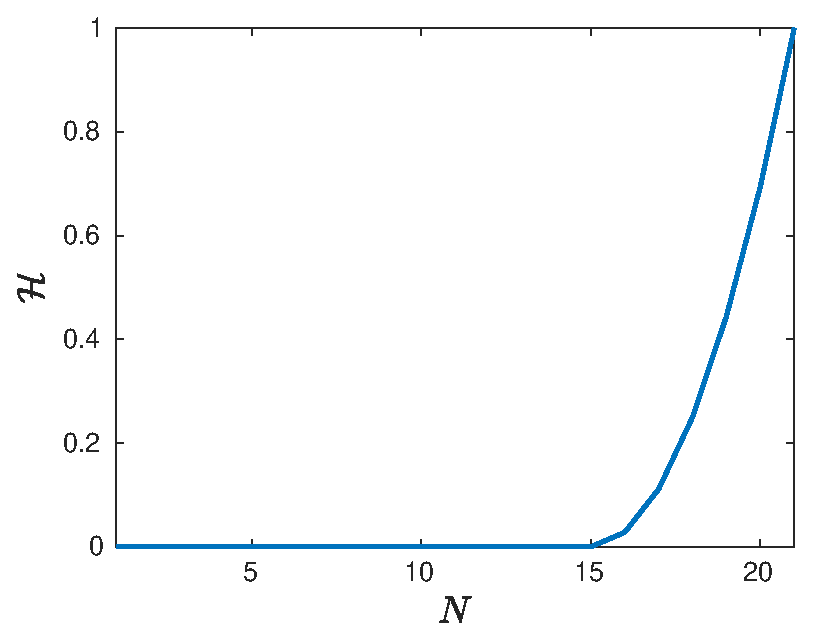
\includegraphics[width=0.60\textwidth]{filter_shape}
	\caption{Transfer function for the spectral coefficients for the filter $\mathcal{H}$ with number of modes $N=21$ and cut-off mode number $N_{c}=16$.}
	\label{fig:filter_shape}
\end{figure}

Several parameter optimization studies were performed to determine the optimum value of $\chi$ and filter shape $\mathcal{H}$ using turbulent channel flow simulations. The LES results were compared with the DNS database of \cite{moser99} and the optimum parameters were further validated for a flow around a wing section at $Re_{c}=400,000$. A good agreement was found between the LES and the DNS data of \cite{hosseini16}, and the optimized parameters were then used for all subsequent simulations.

\section{Arbitrary-Lagrangian-Eulerian (ALE)}

Typical solutions of unsteady fluid flows utilize the Eulerian framework where the coordinate system is fixed in space. A fixed coordinate system however becomes infeasible when the domain boundaries are in motion, as is the case of fluid-structure interaction problems, or when there is a free surface which may lead to a deforming interface. An appropriate method is needed to account or the motion of the boundaries and/or the interior grid points. One such method which substantially simplifies the difficulties arising out of moving boundaries is the Arbitrary-Lagrangian-Eulerian (ALE) method. The method was proposed in a finite-difference framework by \cite{hirt74} and later brought to the spectral-element framework by \cite{ho90,ho91}. The technique combines both the Lagrangian and Eulerian formulations such that, the Navier--Stokes may be solved with the grid points moving with the fluid elements \textit{i.e.} in a Lagrangian framework, or with fixed grid points (Eulerian), or with grid points moving in an arbitrary prescribed manner. The heart of the technique lies in the formulation of the total time rate of change of a quantity in the ALE frame, defined analogously to the material derivative. Thus for a quantity $\mathbf{F(x_{i},t)}$, the change due to small increments $dx_{i}$ and $dt$ may be expressed as \citep{kundu02}
\begin{align}
	dF = \frac{\partial F}{\partial t}dt + \frac{\partial F}{\partial x_{i}}dx_{i}.
	\label{eqn:material_deriv_df}
\end{align}
One may choose to follow any arbitrary path along which this quantity is evaluated, in which case the quantities $dx_{i}$ and $dt$ are related by the velocity of the (grid) point along this arbitrary path $w_{i} = dx_{i}/dt$. The relation results in the expression referred to as the ALE derivative \citep{deville02}, here denoted as $\delta F/\delta t$ to differentiate it from the very similar expression for the material derivative (which is evaluated along the fluid particle trajectory)
\begin{align}
\frac{\delta F}{\delta t} = \frac{\partial F}{\partial t} + w_{i}\frac{\partial F}{\partial x_{i}}.
\label{eqn:ale_derivative}
\end{align}
When $w_{i}$ is equal to the fluid velocity $u_{i}$, we recover the familiar Lagrangian expression for the material derivative $DF/Dt$. On the other hand, when $w_{i}=0$, we get the local (Eulerian) rate of change of the quantity $F$. The material derivative and the ALE derivative share a simple relationship defined using a relative velocity of the fluid particle with respect to the grid motion $c_{i} = u_{i} - w_{i}$, which may be used in the definition of material derivative to obtain
%\begin{subequations}
	\begin{align}
%	\frac{DF}{Dt} = \frac{\partial F}{\partial t} + u_{i}\frac{\partial F}{\partial x_{i}} \nonumber\\
%	\frac{DF}{Dt} = \bigg(\frac{\partial F}{\partial t} + w_{i}\frac{\partial F}{\partial x_{i}}\bigg) + c_{i}\frac{\partial F}{\partial x_{i}} \nonumber \\	
	\frac{DF}{Dt} = \frac{\delta F}{\delta t} + c_{i}\frac{\partial F}{\partial x_{i}}.
	\label{eqn:ale_material_derivative}
	\end{align}
%\end{subequations}
Thus the Navier--Stokes in the ALE formulation may be expressed as 
\begin{subequations}
	\label{eqn:ale_navier_stokes}	
	\begin{align}
	\frac{\delta u_{i}}{\delta t} + (u_{j} - w_{j})\frac{\partial u_{i}}{\partial x_{j}} =  - \frac{1}{\rho}\frac{\partial p}{\partial x_{i}} + \frac{1}{Re}\bigg(\frac{\partial^{2} u_{i}}{\partial x_{j}\partial x_{j}}  \bigg) +f_{i}, \\
	\frac{\partial u_{i}}{\partial x_{i}} = 0,
	\end{align}
\end{subequations}
where $w_{j}$ is the velocity of the grid points. The solution of the Navier--Stokes is then a simple matter of evaluating a suitable grid velocity. 

In many cases, such as the flow over an oscillating airfoil, the velocity of the grid points at the boundary (airfoil surface) may be explicitly known. \cite{ho90,ho91} propose to extend this velocity to the interior points of the domain by solving an elliptic problem for the mesh velocity. In the present work we take a simpler approach to prescribing the mesh velocities in the interior domain. Recognizing the simple trigonometric form of a harmonic pitching motion, all mesh points may simply be prescribed a solid body rotation with the instantaneous angular velocity of the airfoil. However a pure solid-body rotation would also displace the domain boundaries. Therefore a damping function is used to smoothly reduce the rotational velocity away from the airfoil boundary such that the mesh motion is zero at the far-field, inlet and outflow boundaries. Thus for an airfoil with an instantaneous rotation rate of $\Omega_{z}(t)$, the mesh velocity is prescribed as:
\begin{align}
	w_{i}(x,y,z,t) = \underbrace{(\Omega_{z}(t) \times \vec{R})}_{\text{Solid body rotation}} \overbrace{f(|\ \vec{r}\ |)}^{Damping}
	\label{eqn:mesh_velocity}
\end{align}
where $\vec{r}$ is the normal distance of a grid point from the airfoil surface, $\vec{R}$ is the distance from the rotational axis and $f(r)$ is a damping function which can be prescribed in many different ways, depending on one's preferences. The damping function needs to have two essential properties, \textit{i.e.} it must be equal to 1 when $|\vec{r}|=0$, which implies the mesh points at the airfoil boundary move with the surface (solid body rotation at the airfoil surface), and it must smoothly decay to zero close to the far-field boundaries, which allows the external boundaries of the computational domain to remain fixed in physical space. Figure~\ref{fig:mesh_rotation_damping} shows the damping function used in the present work as a function of the normal distance from the airfoil surface.
\begin{figure}[h]
	\centering
	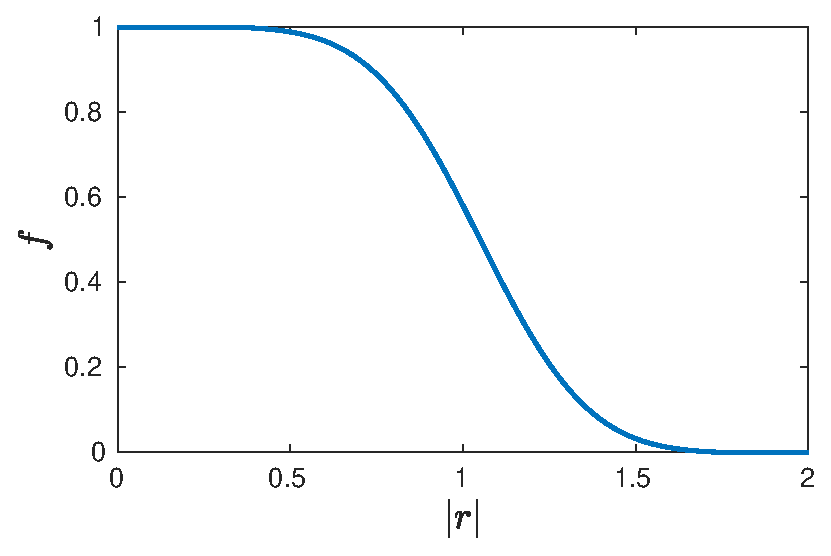
\includegraphics[width=0.55\textwidth]{damping_func}
	\vspace{5pt}
	\caption{Damping function $f(r)$ for the mesh velocities.}
	\label{fig:mesh_rotation_damping}
\end{figure}
The damping function moves the grid points close to the airfoil surface with the same rotational velocity of the airfoil and spreads out the mesh deformation into the interior of the domain. This damping function is calculated once at the beginning of the simulation. Hence all quantities $\Omega_{z}(t),\ \vec{r},\ f(r)$ which are needed for prescribing the mesh velocity are explicitly known at each time-step without the need for solving an elliptic equation as in \cite{ho90,ho91}. 

\section{Free-stream turbulence}

Isotropic, homogeneous free-stream turbulence is prescribed at the inlet and far-field boundaries to add small disturbances to the flow-field, which simulate the disturbances found in a wind-tunnel or in free-flight conditions. The free-stream turbulence is prescribed as a superposition of Fourier modes with a random phase shift. The maximum and minimum amplitudes of the wavenumber vector are prescribed quantities and are limited by the resolution of the spatial discretization and size of the domain respectively. The wavenumber space between the minimum and the maximum is divided into 20 concentric shells with each shell representing the amplitude of the three-dimensional wavenumber vectors lying on the shell. 20 points are randomly chosen on each shell with the location of each point representing the three-dimensional components of the wavenumber vector. Thus the free-stream turbulence is represented by a total of 400 fourier modes. Care is taken to avoid very small wavenumber components which result in wavelengths in physical space that are larger than the computational domain. The streamwise length scales are transformed to a temporal frequency by invoking Taylor's frozen turbulence hypothesis and using the local mean streamwise velocity at the inlet for the space-time conversion. The amplitude of the free-stream modes on each spherical shell is scaled using the von K\'arm\'an spectrum. Figure~\ref{fig:fst_duct} shows an instantaneous visualization of the streamwise velocities in a doubly-periodic duct flow case with high ($5\%$) free-stream turbulence intensity prescribed at the the inlet. Figure~\ref{fig:ti_decay} shows the spatial decay of turbulence intensity. After a small initial distance of adjustment from the inlet, the turbulence intensity decays as a power law. A very similar method for generating free-stream turbulence for simulations of flat-plate boundary layers is used by \cite{schlatterdiploma,brandt04,schlatter08} and more recently for wind turbine simulations by \cite{kleusberglicenciate}.

\begin{figure}[h]
	\centering
	\begin{subfigure}[t]{0.49\textwidth}
		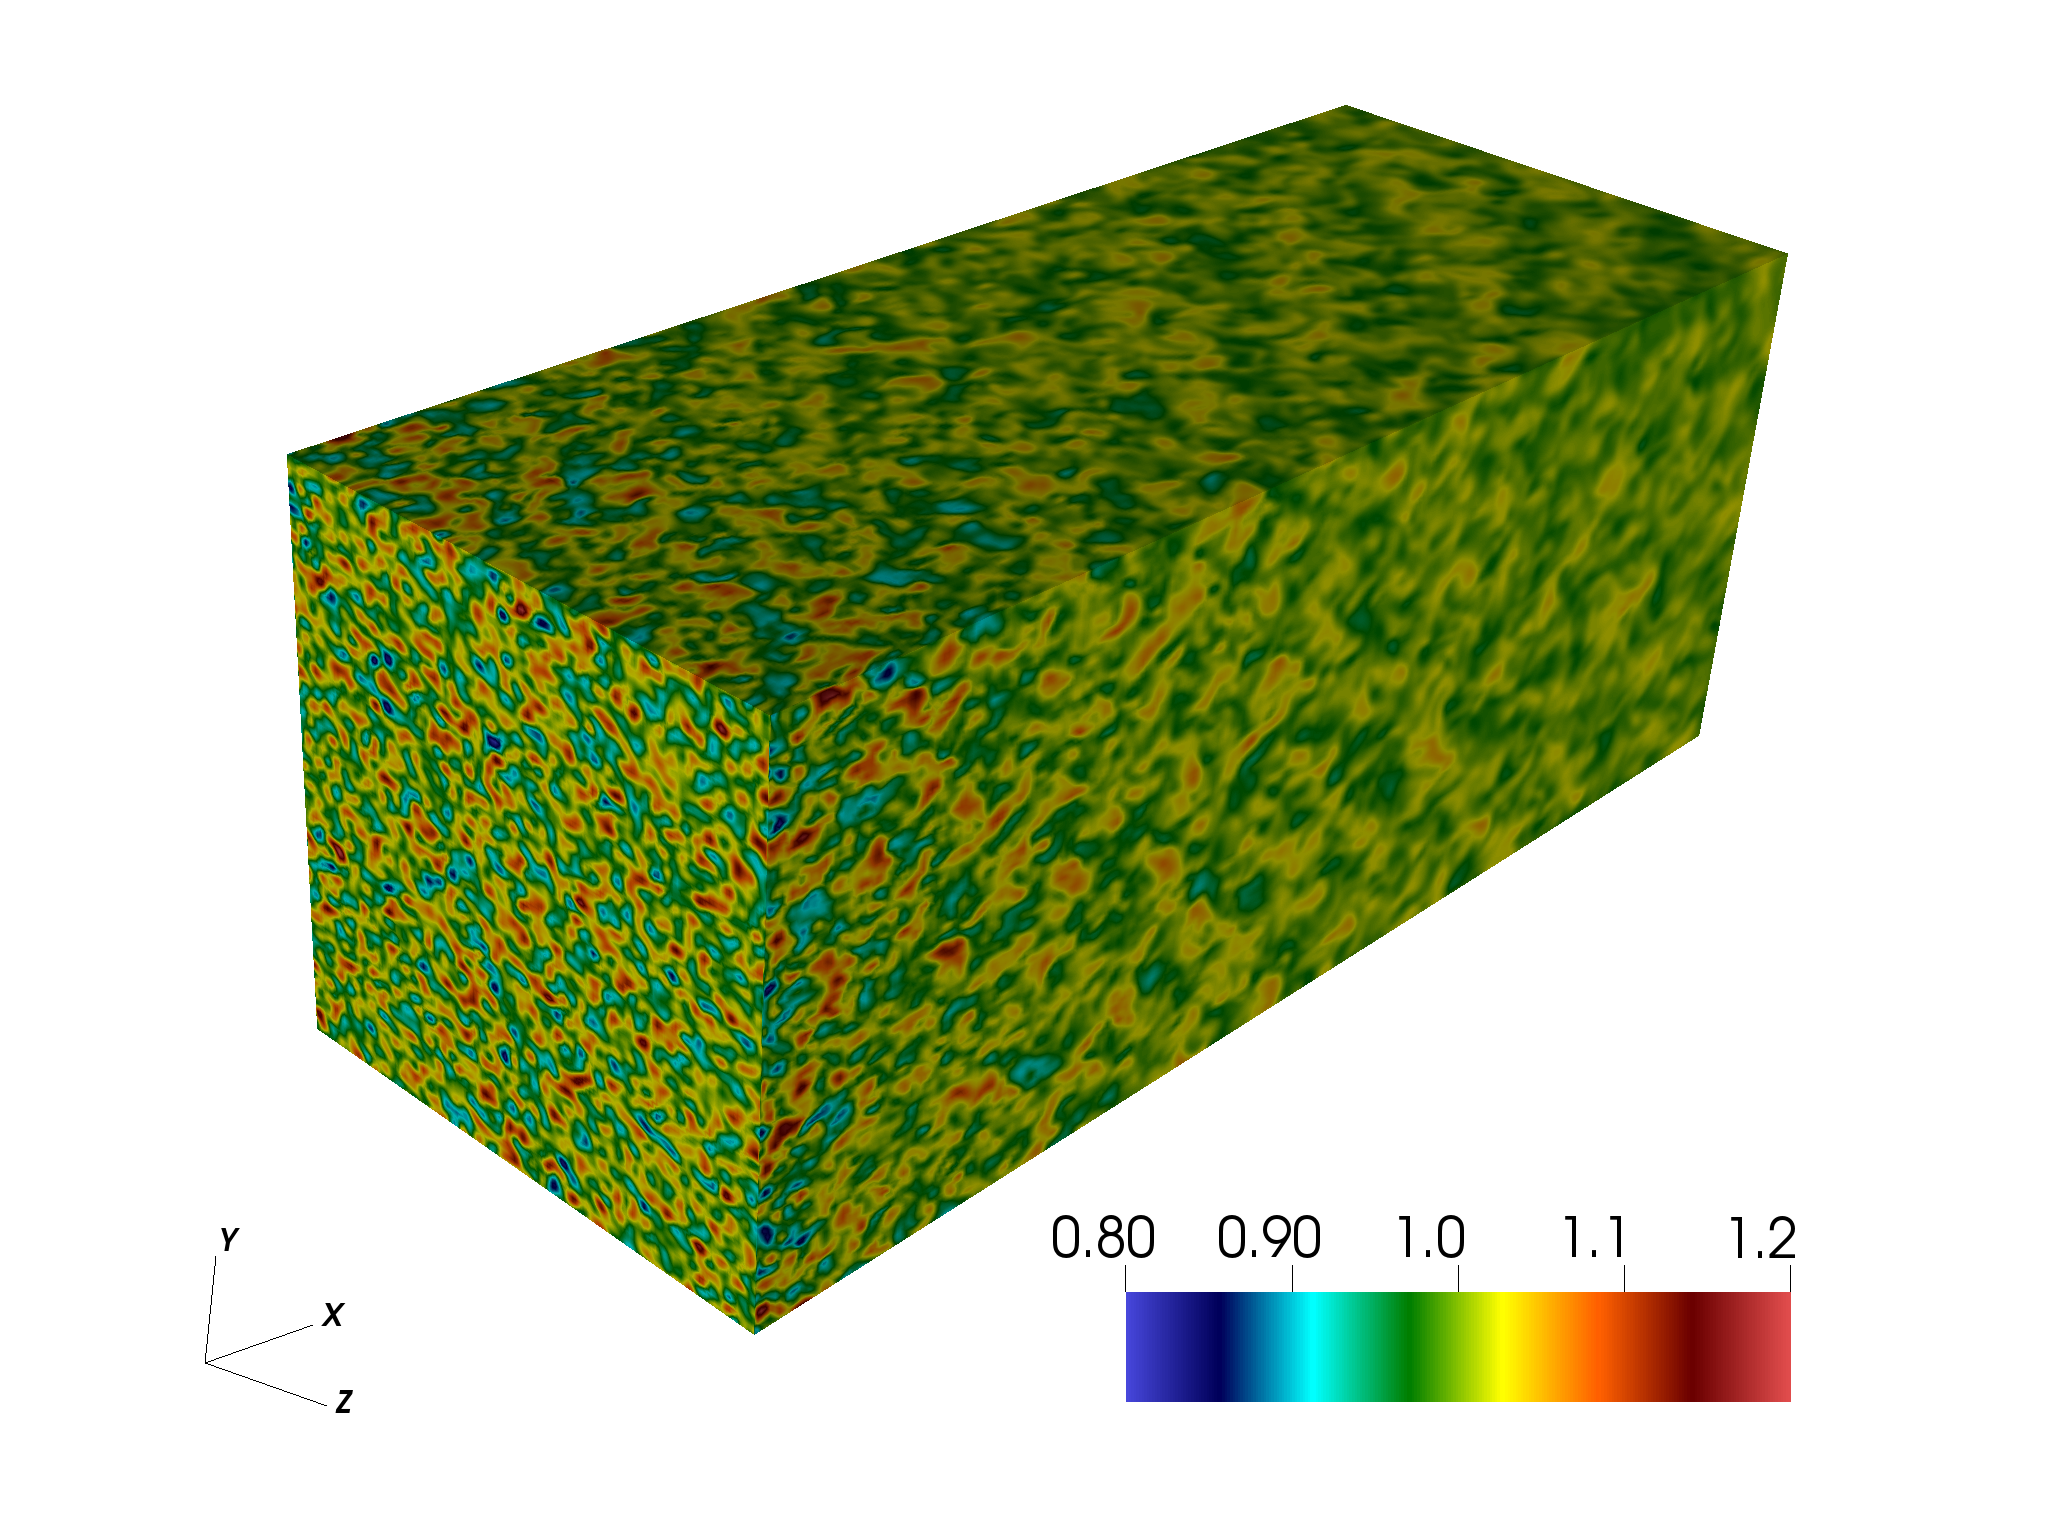
\includegraphics[width=1\textwidth]{fst_duct_vx0000.png}
		\caption{Visualization of free-stream turbulence prescribed at the inlet for a doubly periodic duct flow. Colors represent the instantaneous streamwise velocity.}
		\label{fig:fst_duct}
	\end{subfigure}
	\begin{subfigure}[t]{0.49\textwidth}
		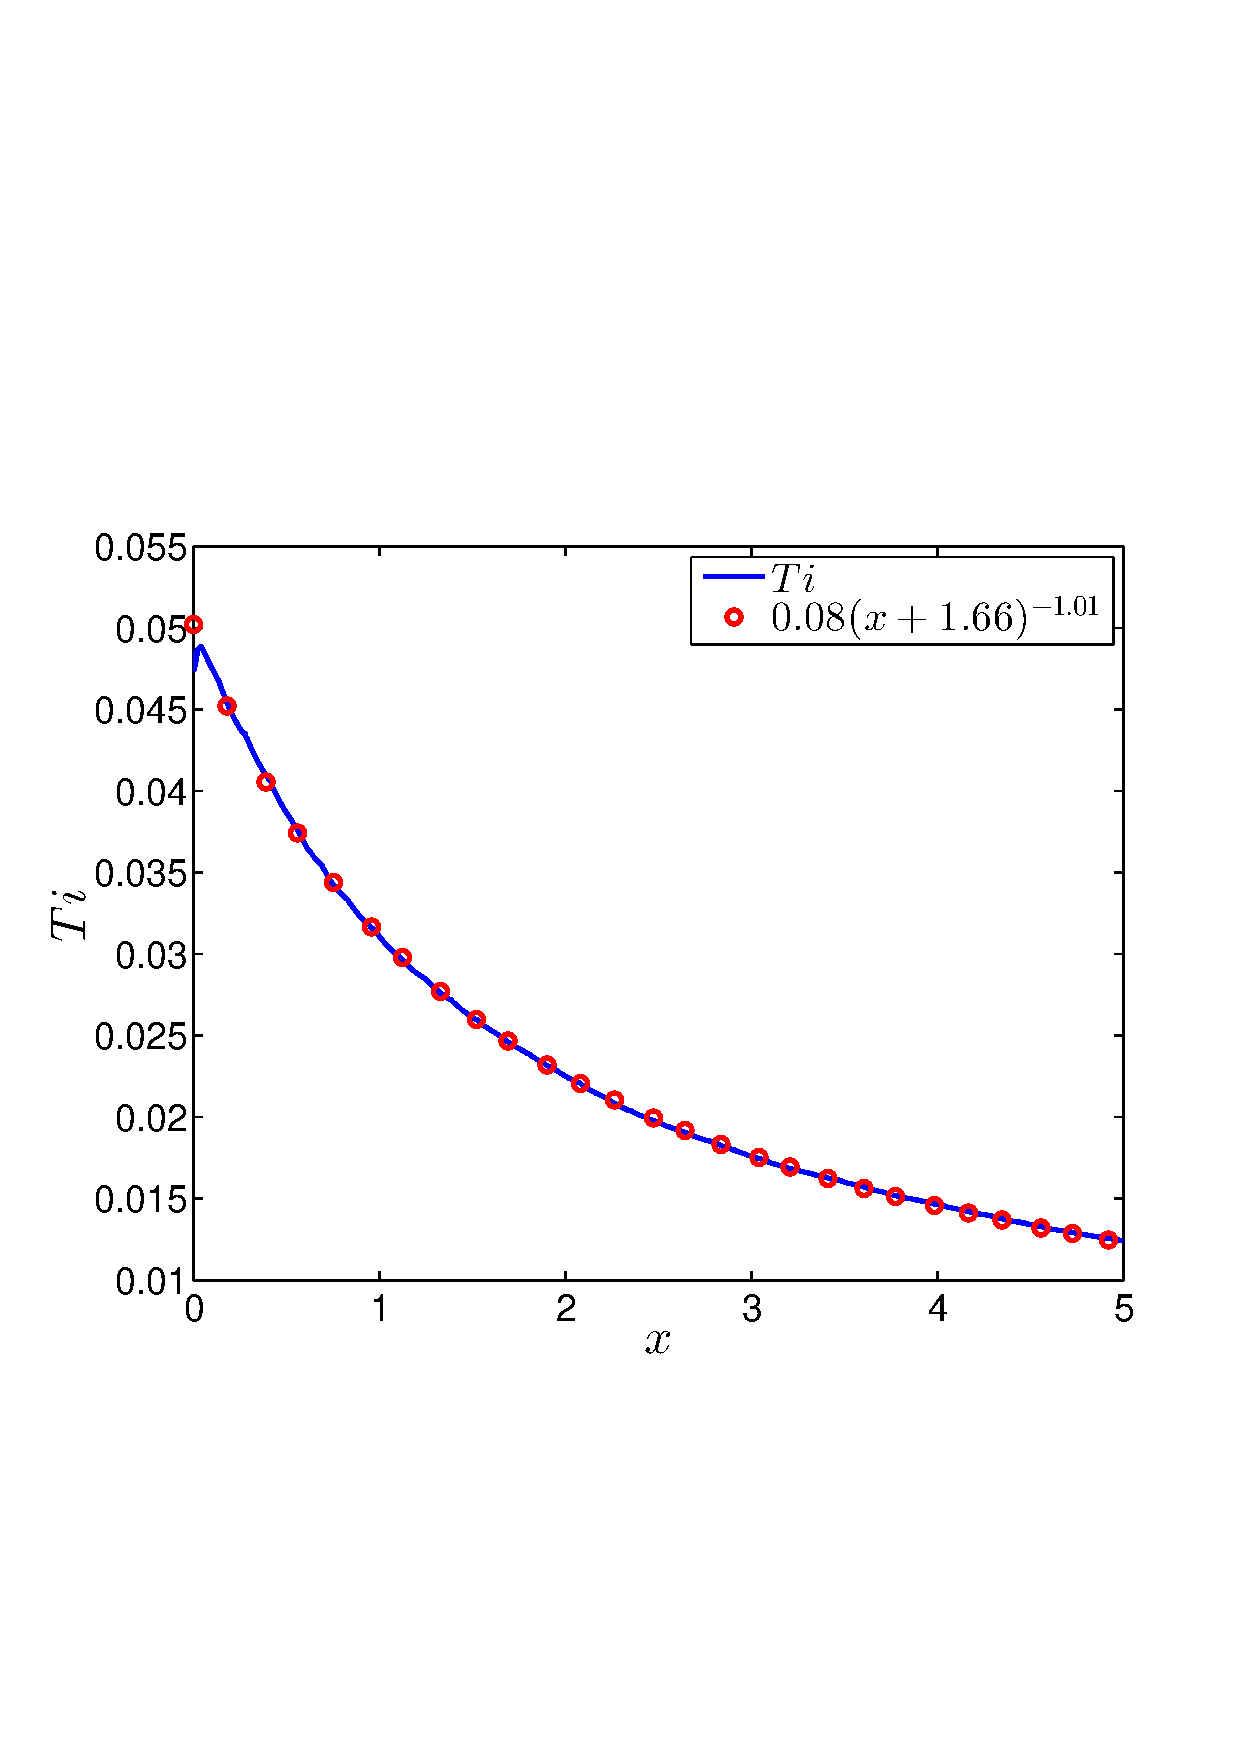
\includegraphics[width=1\textwidth]{ti_decay}
		\caption{Decay of turbulence intensity with streamwise distance, along with the least-squares fit of a power law.}
		\label{fig:ti_decay}
	\end{subfigure}
\end{figure}

%===============================================================================
\chapter{Overview of numerical simulations}
%===============================================================================

\section{Flow around unsteady wings}

The unsteady experiments of \cite{mai11,hebler13} and \cite{lokattthesis} have shown that aerodynamic non-linearities are related to the movement of transition over the suction side of the airfoil. Thus unsteady boundary layer dynamics play an important role in aerodynamic response of NLF airfoils. The present work investigates the unsteady boundary layers with a particular focus on unsteady transition with the aim to shed light on the phenomenon of non-linear unsteady aerodynamic response. The airfoil used in the investigation is the ED36F128 (with a $13.8^{\circ}$ flap deflection), designed at the Aeronautical and Vehicle Engineering department at KTH. It is a natural laminar flow airfoil, which has been used in several steady and unsteady experiments \citep{lokatt17,lokattthesis}. The unsteady experiments have shown the non-linearities that appear to be typical of laminar airfoils \citep{lokattthesis}. The results of the steady and unsteady experiments using this airfoil have been made available to us by Dr. Eller and Dr. Lokatt. Non-linearities in the unsteady aerodynamic forces are observed for only a certain range of angle of attack $\alpha$. Therefore a careful assessment of the data was needed in order to select the right parameter range where the relevant flow physics could be observed in the numerical simulations. The data in the experimental campaign was gathered primarily through pressure taps located around airfoil for the calculation of unsteady aerodynamic forces. Thus measurements of the unsteady boundary layer characteristics was not available through the experimental data. Calculations using an integral boundary layer code XFOIL \citep{drela89}, were used to complement the experimental data and better evaluate the state of the boundary layer in the static measurements.

Figure~\ref{fig:tr_xfoil_100_750} shows the calculated transition locations for two different Reynolds numbers ($Re_{c}=100,000$ and $Re_{c}=750,000$) using XFOIL and figure~\ref{fig:765k_static_cz_foil} shows the experimentally measured normal force coefficient as well as calculations from XFOIL for $Re_{c}=750,000$. For the higher Reynolds number case, transition location varies sharply with angle of attack within the range $3.4^{\circ}<\alpha<6.5^{\circ}$. Aerodynamic non-linearities can also be observed approximately within the same angle of attack range (figure~\ref{fig:765k_static_cz_foil}). For the lower Reynolds number case, no experimental data is available. Therefore solely XFOIL calculations are used and the parameter range is selected where the transition location varies rapidly with angle of attack. This is found for an angle of attack range of $6.7^{\circ}<\alpha<8.0^{\circ}$.
\begin{figure}[!h]
	\centering
	\begin{subfigure}[t]{0.45\textwidth}
		\caption{}
		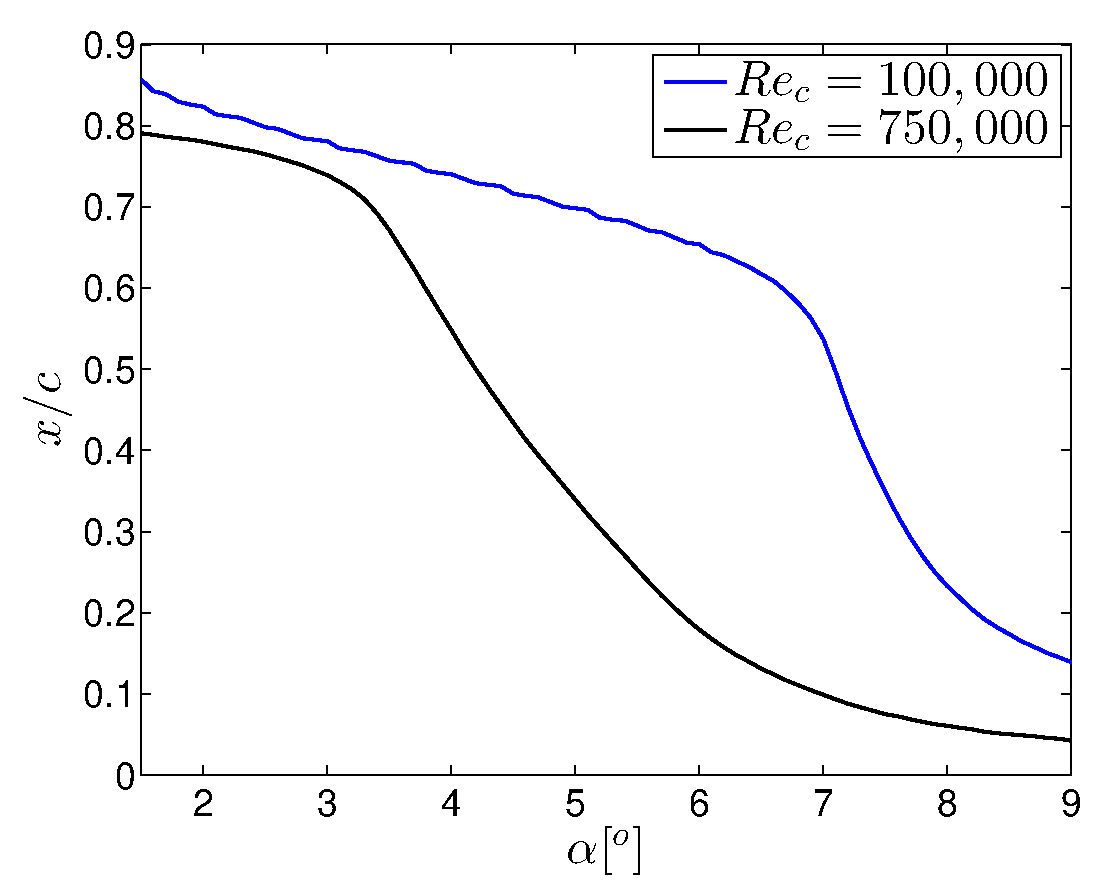
\includegraphics[width=1\textwidth]{tr_xfoil_100_750}
		\label{fig:tr_xfoil_100_750}		
	\end{subfigure}
	\begin{subfigure}[t]{0.45\textwidth}
		\caption{}
		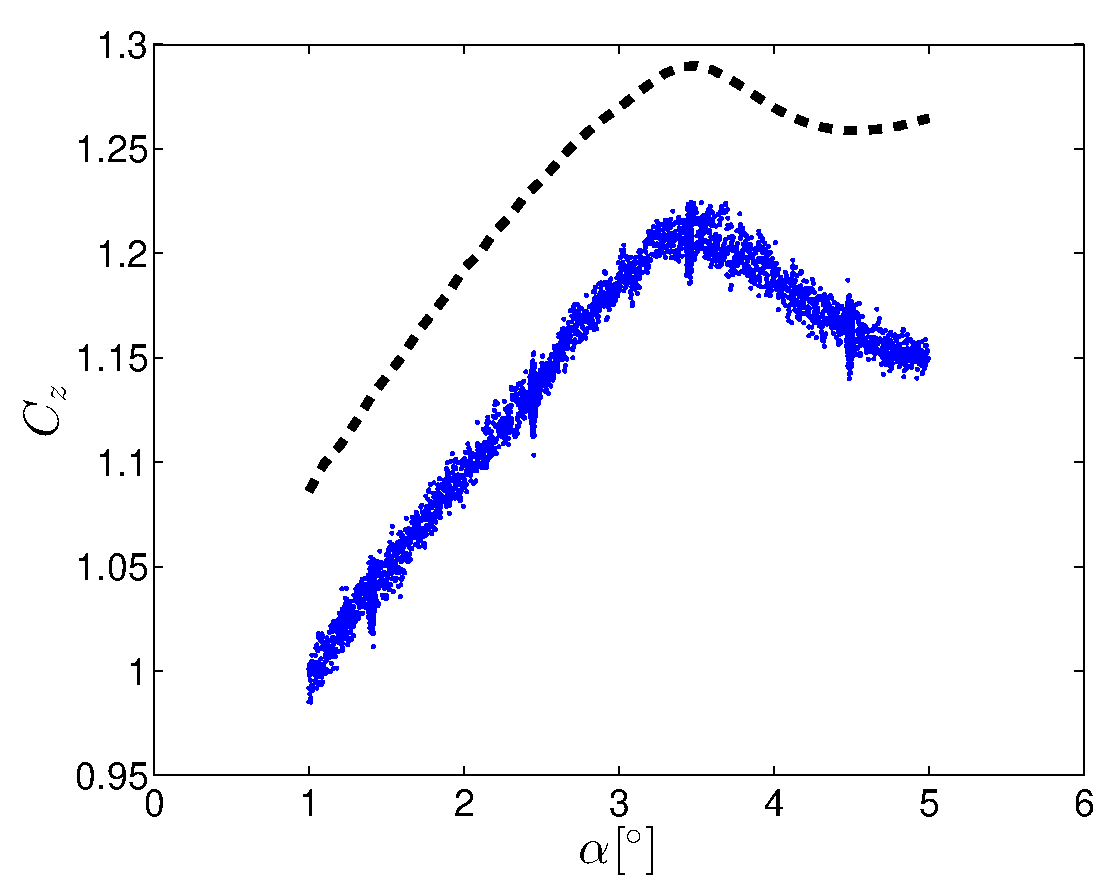
\includegraphics[width=1\textwidth]{765k_static_model_cz_xfoil}
		\label{fig:765k_static_cz_foil}
	\end{subfigure}
	\caption{(a) Transition location calculated using XFOIL for two different Reynolds numbers. (b) Normal force coefficient measured in experiments (dots) and from XFOIL calculations (dashed line) for $Re_{c}=750,000$.}		
\end{figure}
Numerical simulations are performed with stationary airfoils to ensure the expected static boundary layer characteristics are captured by the numerical simulations.  Figure~\ref{fig:overview_la2_750k_stationary} depicts the instantaneous vortical structures in the flow for $Re_{c}=750,000$ for an angle of attack $\alpha=2.4^{\circ}$ and $\alpha=4.4^{\circ}$ which shows the change in boundary layer characteristics in the static cases. Similarly, figure~\ref{fig:overview_isocontour_aoa} shows the static boundary layer characteristics for $Re_{c}=100,000$ at $\alpha=6.7^{\circ}$ and $\alpha=8.0^{\circ}$.
\begin{figure}[h]
	\centering
	\begin{subfigure}[t]{0.49\textwidth}
		\caption{$\alpha=2.4^{\circ}$}		
		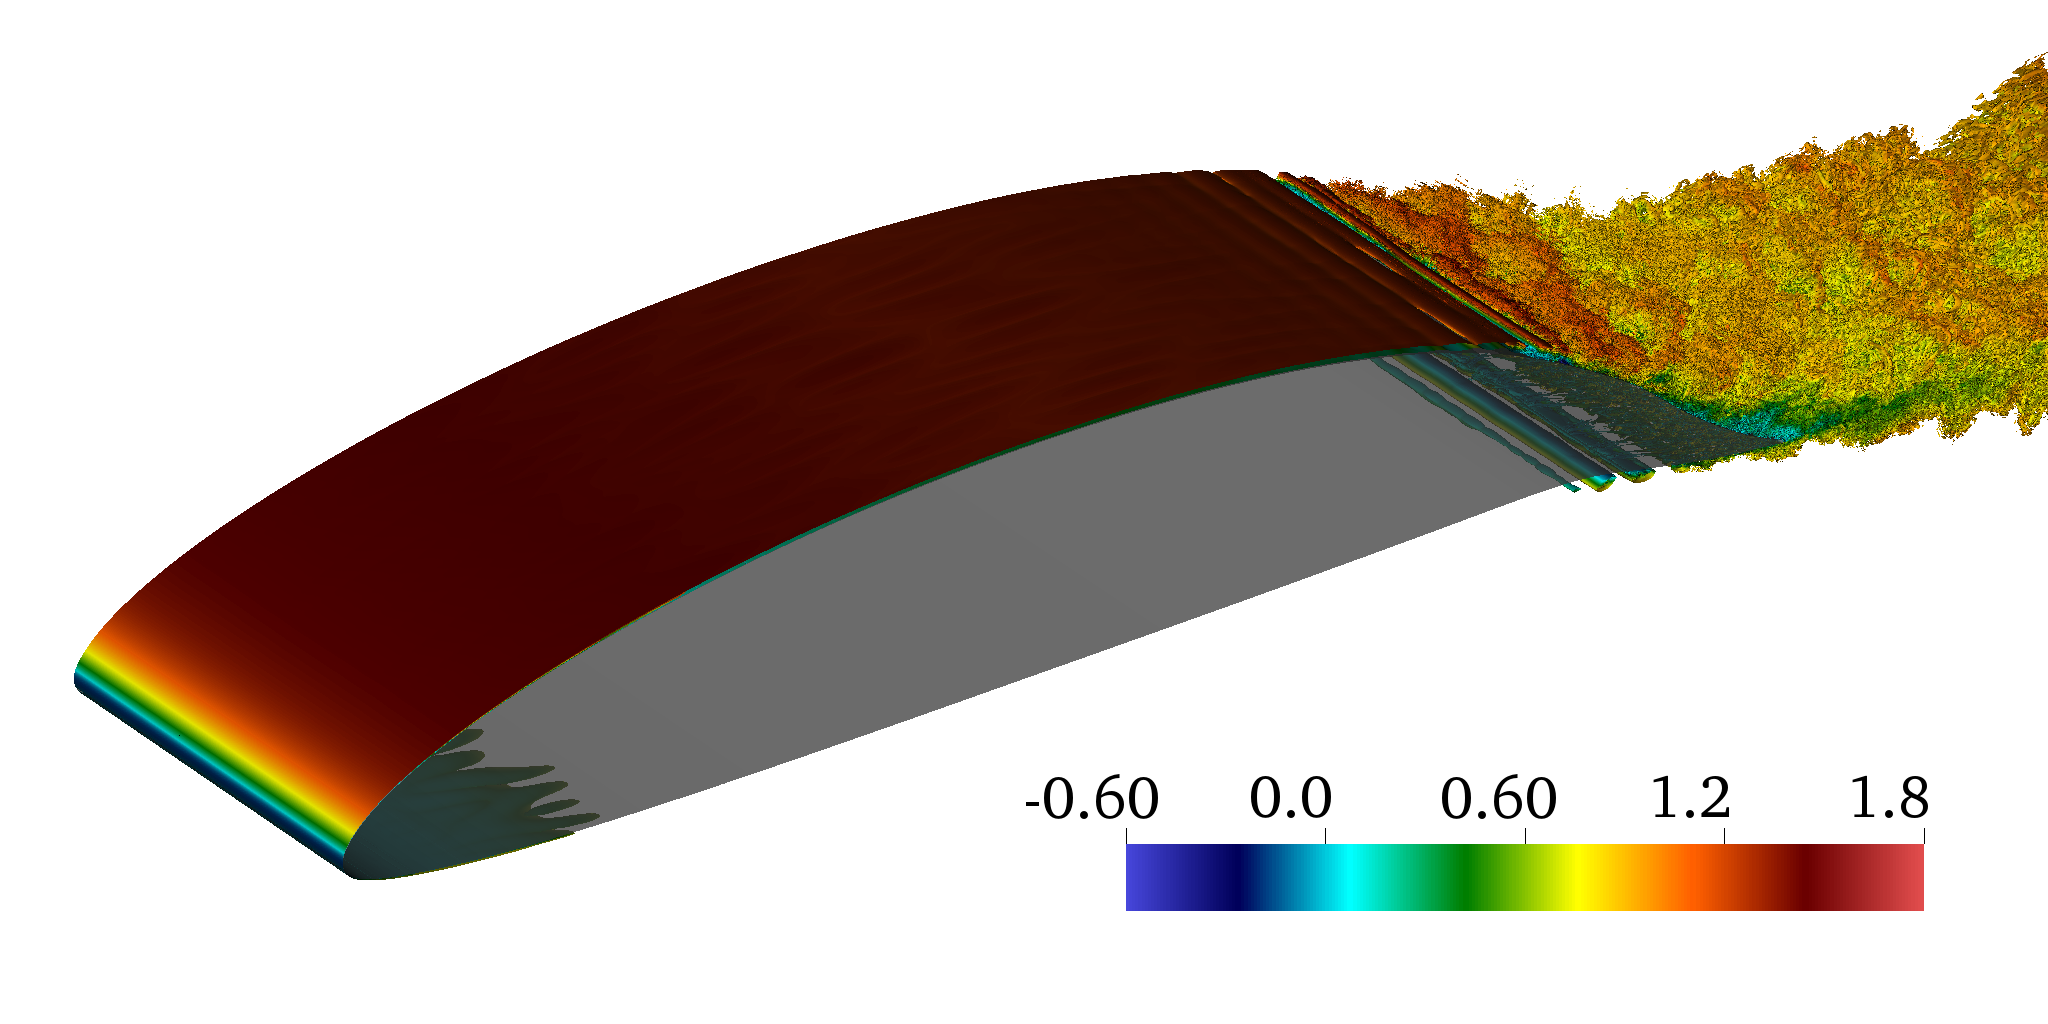
\includegraphics[width=1\textwidth]{paper2/imgs2/pitch_re750k0001}
		\label{fig:overview_la2_aoa24}
	\end{subfigure}
	\begin{subfigure}[t]{0.49\textwidth}
		\caption{$\alpha=4.4^{\circ}$}		
		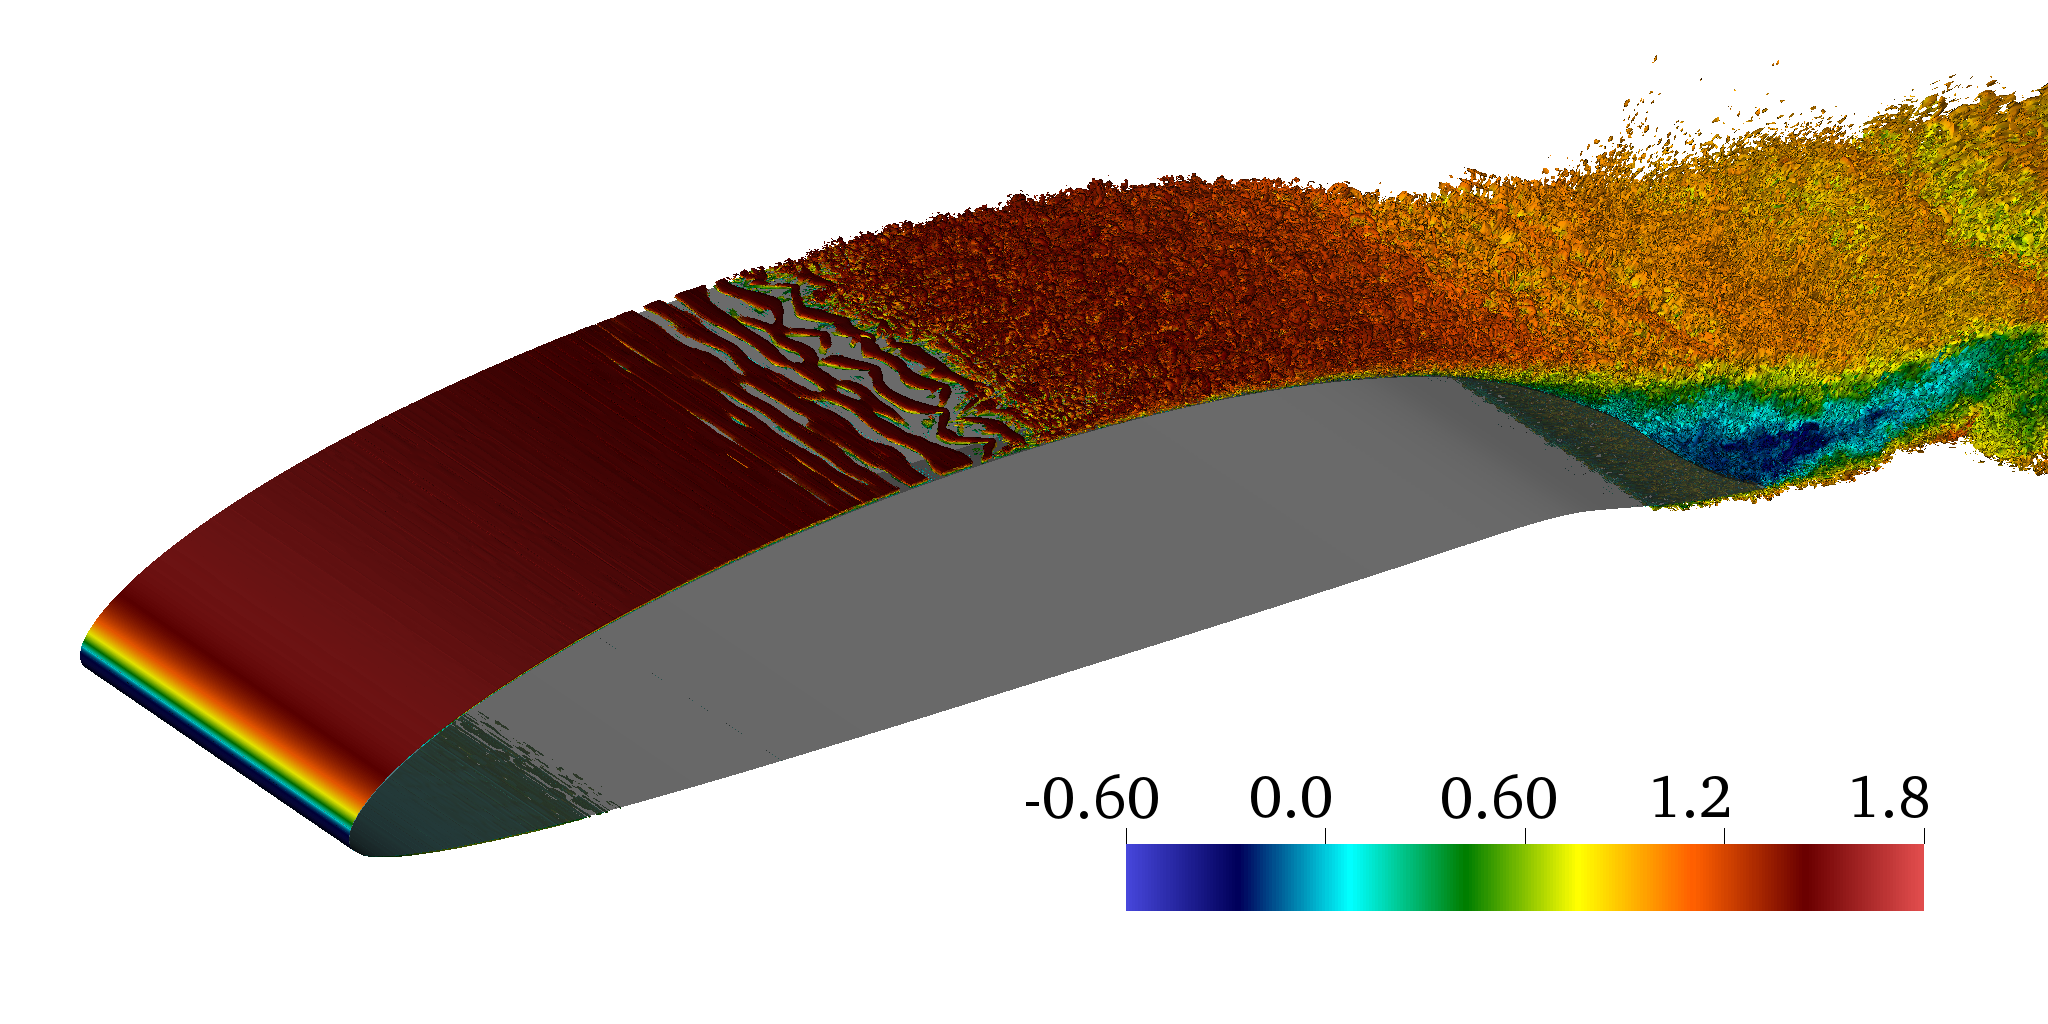
\includegraphics[width=1\textwidth]{paper2/imgs2/pitch_re750k0002}
		\label{fig:overview_la2_aoa44}		
	\end{subfigure}	
	\caption{Instantaneous vortical structures identified by the $\lambda_{2}$ criterion for the two stationary angle of attack simulations at $Re_{c}=750,000$.}
	\label{fig:overview_la2_750k_stationary}
\end{figure}

\begin{figure}[t]
	\begin{subfigure}[b]{0.49\textwidth}
		\centering
		\caption{$\alpha=6.7^{\circ}$}		
		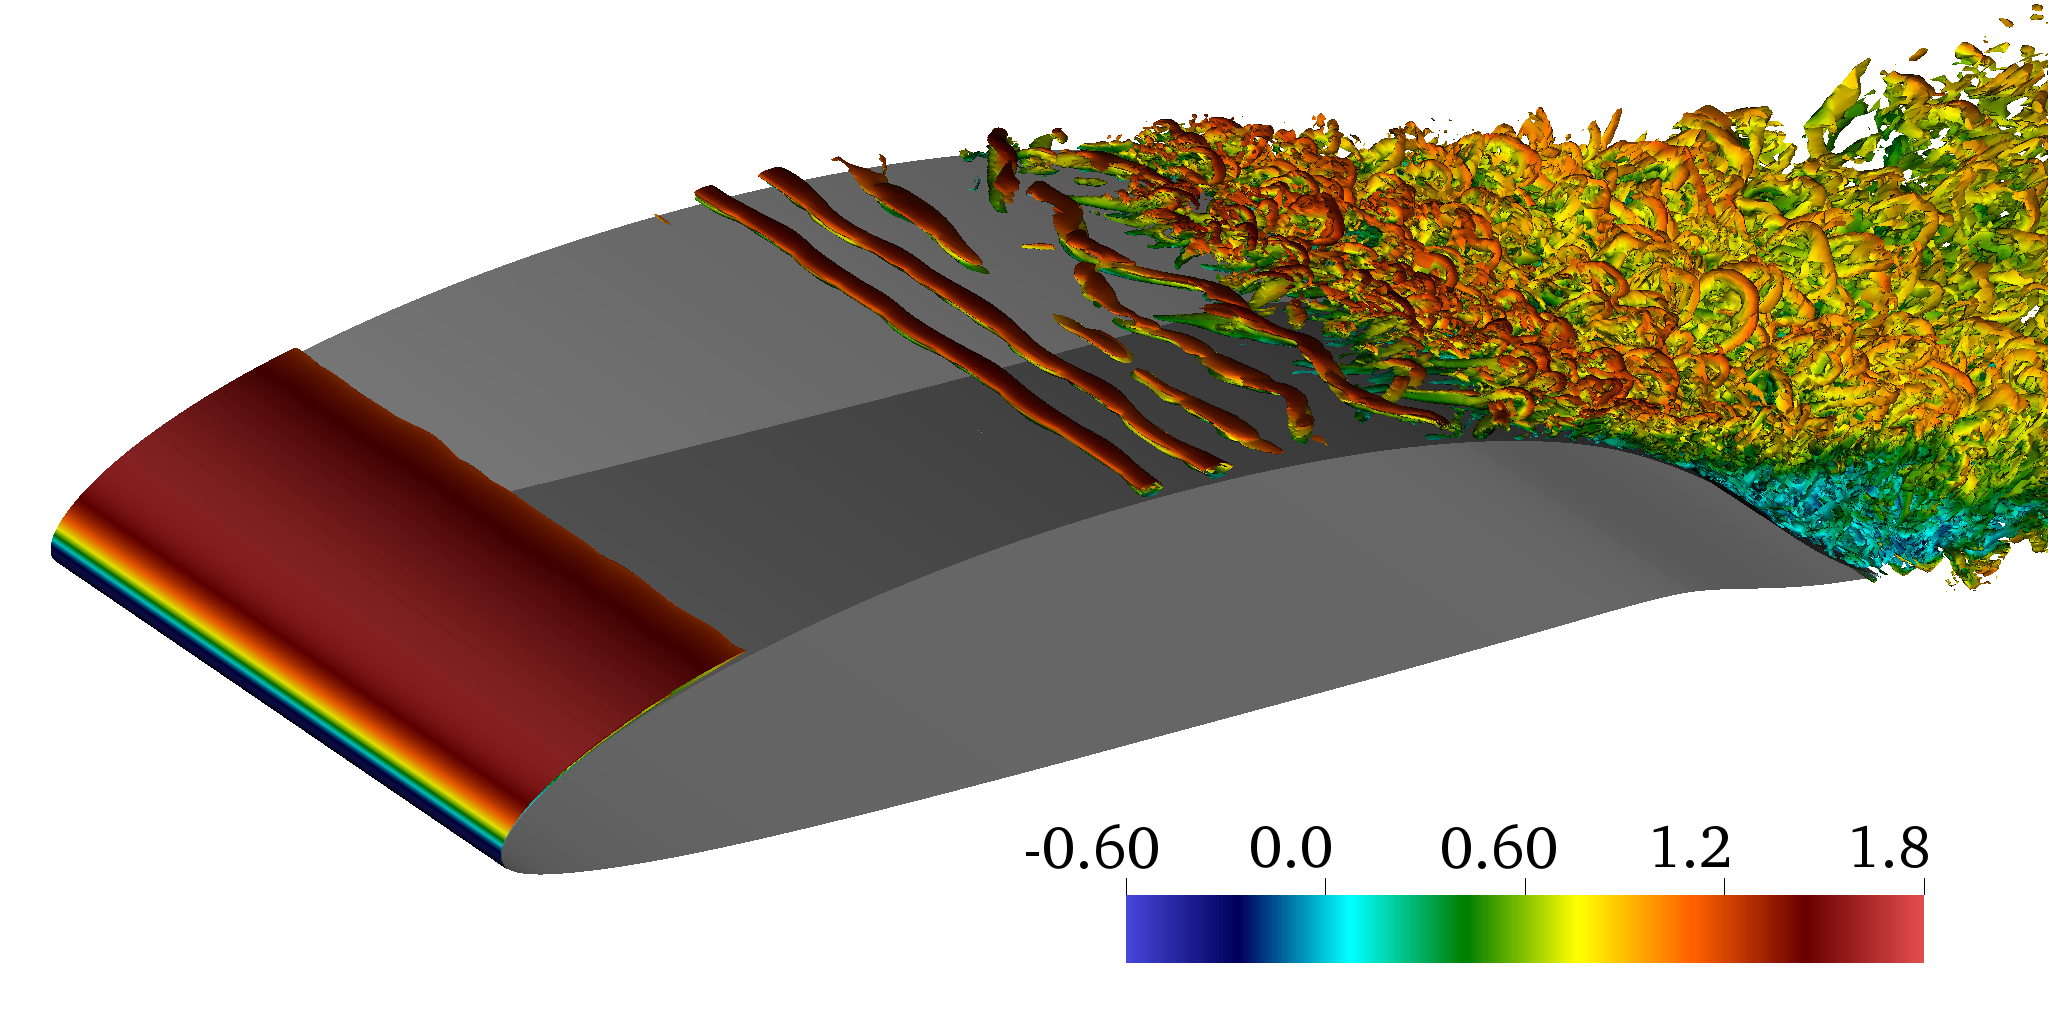
\includegraphics[width=1\textwidth]{paper3/imgs/re100k_static67_0001}
		\label{fig:overview_aoa67_iso}
	\end{subfigure}
	\begin{subfigure}[b]{0.49\textwidth}
		\centering
		\caption{$\alpha=8.0^{\circ}$}		
		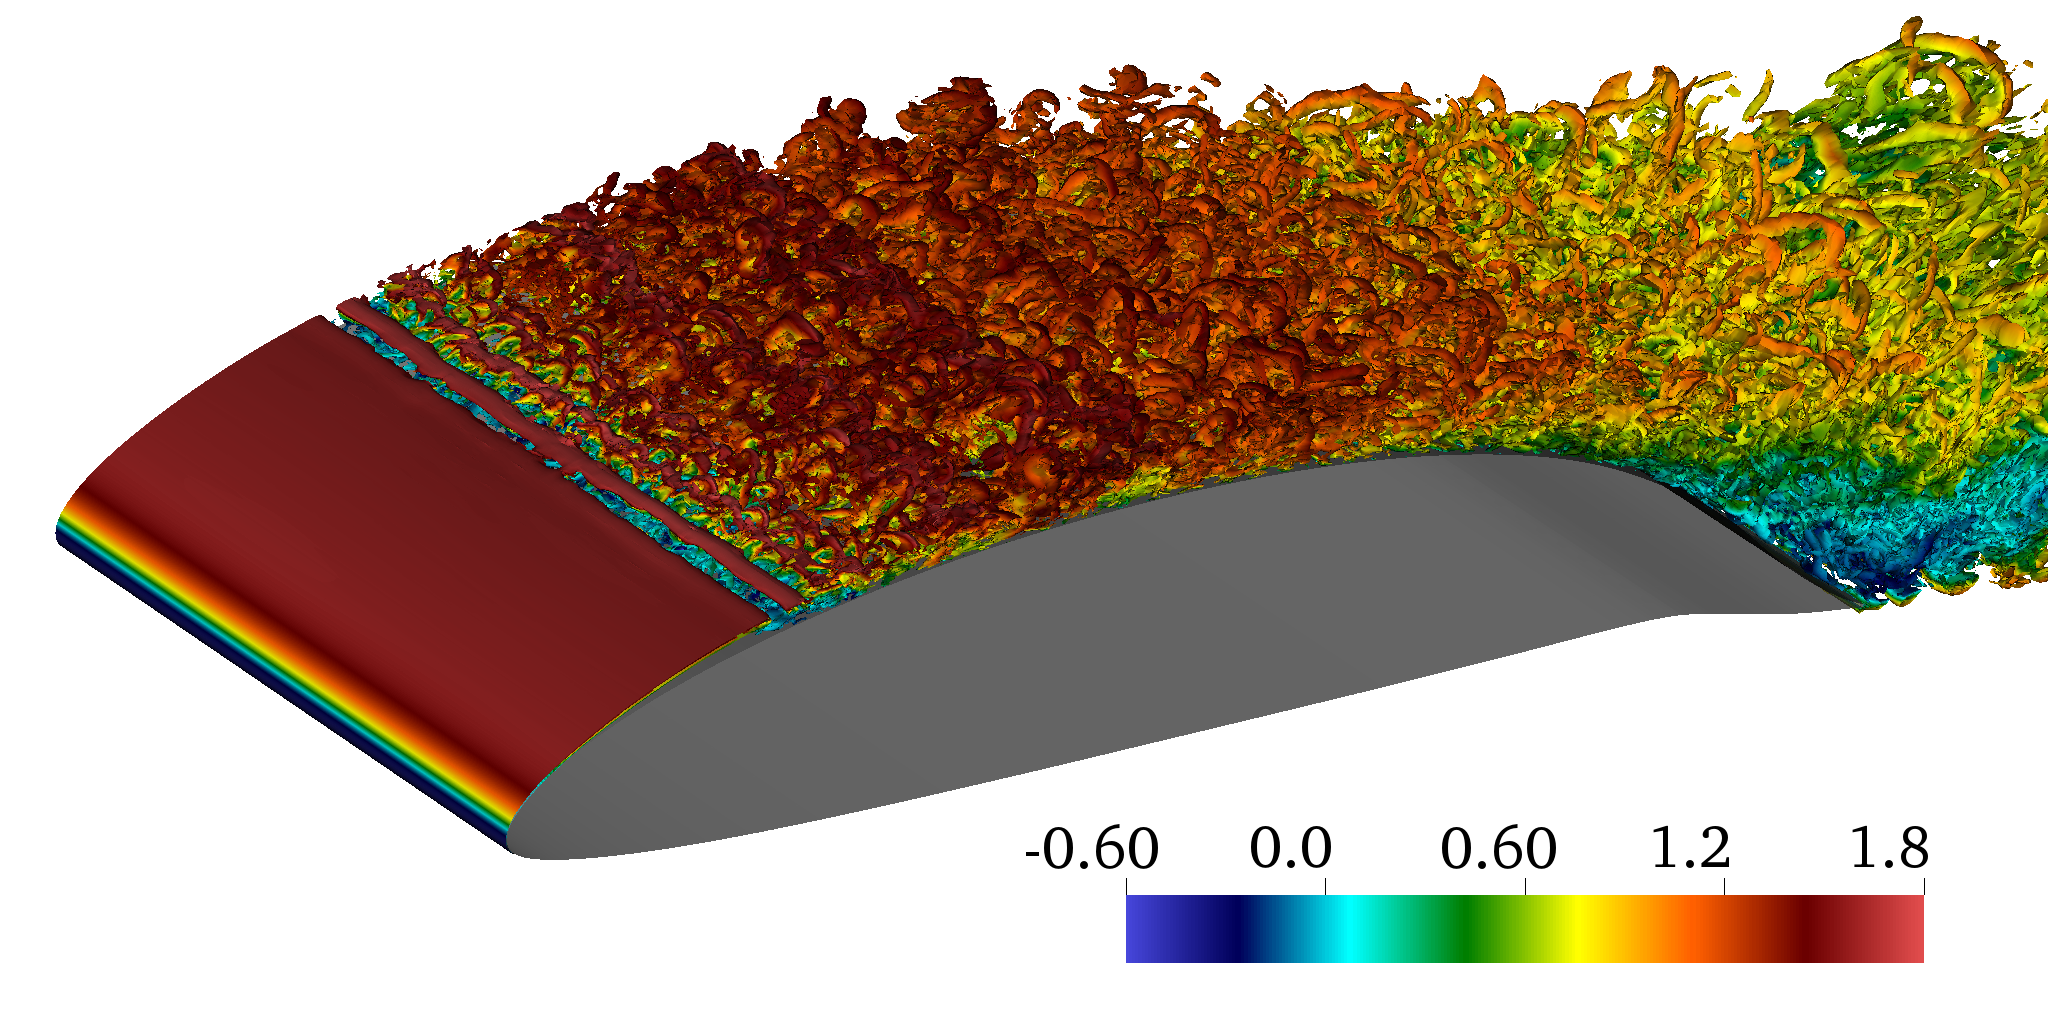
\includegraphics[width=1\textwidth]{paper3/imgs/re100k_static80_0001}
		\label{fig:overview_aoa80_iso}
	\end{subfigure}
	\caption{Isocontours of instantaneous $\lambda_{2}$ structures observed for two different (stationary) angles of attack at $Re_{c}=100,000$.}
	\label{fig:overview_isocontour_aoa}
\end{figure}

For both the Reynolds number cases, significant temporal variation of transition location is also found for the unsteady cases. Figure~\ref{fig:overview_transition_alpha} shows the variation of transition with respect to $\alpha$. The transition locations were calculated using thresholds on the instantaneous spanwise-averaged Reynolds stress $\overline{u'v'}$ and spanwise fluctuation intensity $\overline{w'w'}$. For the lower Reynolds number case the boundary layer also develops a leading-edge laminar separation bubble during the pitch cycle which significantly influences the boundary-layer dynamics.

\begin{figure}[t]
	\begin{subfigure}[b]{0.49\textwidth}
		\centering		
		\includegraphics[width=1\textwidth,height=0.80\textwidth]{imgs/750k_transition_alpha.eps}
	\end{subfigure}
	\begin{subfigure}[b]{0.49\textwidth}
		\centering	
		\includegraphics[width=1\textwidth]{paper3/imgs/transition_alpha.eps}
	\end{subfigure}
	\caption{Phase portraits of transition location for (left) $Re_{c}=750,000$ and (right) $Re_{c}=100,000$.}
	\label{fig:overview_transition_alpha}
\end{figure}


\section{Flow around a stationary wing section}

The final paper in the thesis deals with the study of the boundary layer over a wing section at a chord-based Reynolds number of $Re_{c}=1,000,000$. The airfoil used for the study is the asymmetric NACA 4412. A DNS database for the flow around the same airfoil at $Re_{c}=400,000$ is available and comparisons are made between the two cases to assess the effects of changing Reynolds number on the developing boundary layer. The numerical setup is done in a manner very similar to the computational study by \cite{hosseini16}. Figure~\ref{fig:overview_flow_field_re1000k} shows a section of the numerical grid and the instantaneous vortical structures in the flow field. Figure~\ref{fig:overview_beta_Reth_Ret} shows a comparison of the different measures of the boundary layer over the chord-wise distance for the two different Reynolds numbers. While both wall-shear stress (indicated by $Re_{\tau}$) and boundary layer thickness (measured with momentum thickness Reynolds number $Re_{\theta}$) change between the two cases, the Clauser parameter stays nearly the same throughout the chord. This allows comparisons across different Renolds numbers without ambiguity since the pressure gradient histories remain the same with changing Reynolds numbers. 
\begin{figure}[t]
	\centering
	\includegraphics[width=0.49\textwidth]{paper4/imgs/wing_mesh}
	\includegraphics[width=0.49\textwidth]{paper4/imgs/wing_visualization}
	\caption{(Left) Two-dimensional slice of the computational domain showing the spectral-element distribution. (Right) Instantaneous flow field showing coherent structures identified with the $\lambda_{2}$ method \citep{jeong95}, and colored with horizontal velocity. In this figure, dark blue represents a horizontal velocity of $-0.1$ and dark red a value of $2$.}
	\label{fig:overview_flow_field_re1000k}
\end{figure}

\begin{figure}[t]
	\centering
	\includegraphics[width=0.49\textwidth]{paper4/imgs/beta_vs_x}
	\includegraphics[width=0.49\textwidth]{paper4/imgs/Reth_vs_x}
	\includegraphics[width=0.49\textwidth]{paper4/imgs/Ret_vs_x}
	\caption{Streamwise evolution of (top left) the Clauser pressure-gradient parameter $\beta$, (top right) the Reynolds number based on momentum thickness $Re_{\theta}$ and (bottom) the friction Reynolds number $Re_{\tau}$, for the two wing cases under study.}
	\label{fig:overview_beta_Reth_Ret}
\end{figure}

%===============================================================================
\chapter{Conclusions and outlook}
%===============================================================================

The current thesis work concerns three different fields of research.

In the first part of the thesis, the ``evolve and filter'' technique for the stabilization of spectral-element methods is analyzed and it is found the filter operation causes an undesirable loss of divergence-free quality of the solution. This loss of divergence is shown to be particularly large for the test case of a double shear layer. An alternate formulation of the stabilization called the relaxation-term (RT) stabilization is shown to overcome the drawbacks of the explicit filtering technique, while maintaining the simplicity of the original explicit filter. This RT stabilization technique is very closely related to explicit filtering, with the two operations being equivalent to the leading order in time. Stability limits of the RT stabilization are explored and is shown to be stable within the practical parameter range.

In the second part, an NLF airfoil undergoing small-amplitude pitch-oscillations is analyzed at two different Reynolds numbers. In both cases a large variation of transition, and thus boundary layer characteristics is observed over the airfoil resulting in a non-linear response of the aerodynamic force coefficients. For $Re_{c}=750,000$ it shown that the temporal evolution of the transition point can be understood with a simple phase-lag concept, with the implication that boundary-layer evolution may be considered quasi-steady in time. Using this phase-lag concept a simple empirical model is developed which is able to explain a fairly wide range of experimental data.

On the other hand, for $Re_{c}=100,000$ a qualitatively different picture emerges for the unsteady boundary layer. The boundary-layer response displays a dynamically rich behavior with marked asymmetry of upstream and downstream transition movement. In this case, transition location is governed by the properties of the leading-edge laminar separation bubble (LSB) and it is conjectured that the absolute instability of the LSB may be responsible for abrupt changes in boundary layer characteristics.

Finally, in the third part of the study, flow over a stationary NACA 4412 airfoil is studied at two different Reynolds numbers with the aim of better understanding the boundary-layer evolution in non-equilibrium pressure gradient boundary layers. Two flow cases at a chord-based Reynolds number of $Re_{c}=400,000$ and $Re_{c}=1,000,000$ are compared at different streamwise locations. It is found that the effect of the streamwise pressure gradients is higher at low Reynolds numbers, leading to greater energy in the larger structures present in the outer part of the turbulent boundary layer.

The current work has laid the foundation for several interesting questions that may be the focus of future work. Can the simple empirical aerodynamic model be extended for a wider range of unsteady motions? Can the phase-lag be predicted a-priori as in the case of the classical model by \cite{theodorsen35}? When does the quasi-steady assumption break down and the boundary layer becomes truly unsteady? For $Re_{c}=100,000$, can the asymmetry of the (upstream and downstream) velocities of transition point be linked with the stability properties of the LSB? What is the influence of free-stream turbulence on unsteady LSB? In stationary airfoils, how does the velocity spectrum change with Reynolds number in non-equilibrium flows? What are the characteristics of boundary layer streaks in non-equilibrium flows? Some of these questions will be the focus of further research.


%===============================================================================
% Acknowledgments
%===============================================================================
%
\input{acknowledgements}


%===============================================================================
% References
%===============================================================================
%
\bibliographystyle{jfm}
\bibliography{licentiate}
%
\IfFileExists{overview.bbl}{\input{overview.bbl}}{}
}{}
}{}



%-------------------------------------------------------------------------------
% Comment the following command if you do not want a separate page for Part II
% in the table of contents
%
\tocpagebreak


%===============================================================================
% Part II: Papers
%===============================================================================
%
\part{Papers}

%-------------------------------------------------------------------------------
% Summary of the papers
%
\makepapersummary
\cleardoublepage

%-------------------------------------------------------------------------------
% Paper 1
%
%------------------------------------------------------------------------------
% Define title, author(s), affiliation and publishing status
%
\papertitle[SEM stabilization] % Short title used in headlines (optional)
{%
  A re-examination of filter-based stabilization for spectral-element methods% THE COMMENT SYMBOL AT THE END OF THIS LINE IS NEEDED
}%
%
\papertoctitle{A re-examination of filter-based stabilization for spectral-element methods} % Title for toc
%
\paperauthor[Negi, Schlatter \& Henningson] % Short authors used in headlines and List Of Papers
{%
  P. S. Negi, P. Schlatter and D. S. Henningson%
}%
%
%\listpaperauthor{A. Skywalker \& D. Vader}% (optional) Short authors used in List Of Papers
%
\paperaffiliation
{%
%  $^1$ Linn\'e FLOW Centre, KTH Mechanics, S-100 44 Stockholm, Sweden\\
%  $^2$ Swedish e-Science Research Centre (SeRC), SE-100 44, Stockholm, Sweden%
%  Linn\'e FLOW Centre, KTH Mechanics, S-100 44 Stockholm, Sweden\\
%  Swedish e-Science Research Centre (SeRC), SE-100 44, Stockholm, Sweden%
Department of Mechanics, Linn\'e FLOW Centre and Swedish e-Science Research Centre (SeRC), KTH Royal Institute of Technology, SE-100 44 Stockholm, Sweden 
}%
%
\paperjournal[Tech. Rep] % Short publish info used in List Of Papers
{%
	Technical Report%
}%
%
%\papervolume{42}%
%
%\papernumber{2}%
%
%\paperpages{1--10}%
%
%\paperyear{3639}%
%
\papersummary%
{% Insert summary of the paper here (used in introduction) 
	We revisit the ``filter-based stabilization'' approach proposed by \cite{fischer01} and find that the loss of divergence-free condition due to commutation errors can be particularly severe in the cases of marginally resolved flows. In light of this, an alternative approach based on ``relaxation-term-based stabilization'' is proposed which is closely related to the explicit filter operation. The method retains the advantages of simplicity and efficiency of an explicit filter while also remedying some of its drawbacks. The effect of this relaxation-term is analyzed and it found to be an effective method of stabilization within the practical parameter range. Parameter limits of the stabilization procedure are also presented.
}%
%
\graphicspath{{paper1/imgs/}}%
%
%
%===============================================================================
%                            BEGIN PAPER
%===============================================================================
%
\begin{paper}

\makepapertitle

%------------------------------------------------------------------------------
% Abstract
%------------------------------------------------------------------------------
%
\begin{paperabstract}
	We revisit the ``filter-based stabilization'' approach proposed by \cite{fischer01} and find that the loss of divergence-free condition due to commutation errors can be particularly severe in the cases of marginally resolved flows. In light of this, an alternative approach based on ``relaxation-term-based stabilization'' is proposed which is closely related to the explicit filter operation. The method retains the advantages of simplicity and efficiency of an explicit filter while also remedying some of its drawbacks. The effect of this relaxation-term is analyzed and it found to be an effective method of stabilization within the practical parameter range. Parameter limits of the stabilization procedure are also presented.
\end{paperabstract}


%------------------------------------------------------------------------------
% Article
%------------------------------------------------------------------------------
%

\section{Introduction}

Stability of numerical methods is a well-known challenge. This is particularly true in the case of high Reynolds number ($Re$) flows where low physical dissipation allows small numerical errors to grow in time. Especially if the solution method provides very low numerical dissipation as is the case with high-order methods. A particular type of numerical oscillation arises  due to the violation of the \emph{inf-sup} or Ladyzenskaya-Brezzi-Babu\v{s}ka (LBB) condition. These occur due to inconsistent approximation spaces for the velocity and pressure and are found in both high and low Reynolds number flows. Instabilities specific to high Reynolds number flows have often been associated with the non-linear advection term. These instabilities have been known since \cite{phillips59}, who showed an instability arising due to non-linear interactions within a finite difference scheme. Philips was able to remove the instability by periodically removing energy from half the wavelengths in the simulation. \cite{orszag71} noted that only the highest third of the scales are necessary to be filtered out. The effects of aliasing due to non-linear interactions on the flow quality are discussed in \cite{kirst87,chow03} and \cite{canuto88}. For non-uniform grids, \cite{kirby03} showed improved stability and accuracy of the incompressible Navier--Stokes solutions for spectral-element methods when using consistent integration (over-integration) of the non-linear term. This involves the evaluation of the non-linear term on a higher number of grid points, which provides a complete integration of the term. \cite{malm13} showed that the non-linear advection term is skew-symmetric and an incomplete integration of this term leads to a loss of skew-symmetry. This loss of skew-symmetry causes some of the eigenvalues of the operator to have a positive real part, in turn leading to numerical instability. These works on aliasing, over-integration and skew-symmetry provide valuable insight into the numerical instability associated with the advection term. However the current knowledge of the sources of numerical instability does not appear to be exhaustive. Indeed \cite{malm13} show that one of their test cases suffered from numerical instability despite the use of over-integration. The authors conjecture that even small amounts of errors in divergence would lead to instability. The same test cases were used by \cite{fischer01} where the authors say that they were unable to stabilize the simulation with only over-integration within a reasonable resolution. In light of these issues other methods are necessary to suppress numerical oscillations. One of the earliest methods employed simple addition of a second order dissipative operator by \cite{vonneumann50}. \cite{tadmor89} first proposed the spectral vanishing viscosity (SVV) method for the stabilization of a 1D Burgers' equation. \cite{maday93} used SVV in the context of legendre pseudospectral methods. The method was used for a large-eddy simulation (LES) by \cite{karamanos00} and further shown as a useful stabilization method for spectral element methods \citep{kirby06}. An alternate method that has been proposed in the context of spectral element methods has been that of filter-based stabilization by \cite{fischer01}. Instead of adding a dissipative term to the Navier--Stokes, the method involves a simple two-step procedure of \textit{``evolve one time-step and filter"}. This particular stabilization strategy has been analyzed in some detail by \cite{ervin12}. The filter function is a low-pass filter, built in modal space. The loss of $C_{0}$ continuity which occurs when applying the low-pass filter can be averted by using a simple basis transformation which preserves the physical values at the element boundaries after the application of the filter \citep{boyd98}. This completely negates the need for inter-element information transfer and thus makes the filtering operation local to each spectral-element. The method has been shown to be effective at stabilizing flows even at high Reynolds numbers and the simplicity of the method is highly attractive. However, it suffers from a few potential drawbacks. For one, the \textit{``evolve and filter"} operation is time-step dependent with more energy being filtered out of the system for a smaller time-step since that requires more time-steps to solution and hence more filter applications. Secondly the simple transform procedure introduced by \cite{boyd98} creates a filter operation which is not strictly dissipative and may in some situations be a source of energy in the flow. This was pointed out by \cite{pasquetti02} and also mentioned in the original papaer by \cite{fischer01}. However \cite{pasquetti02} note that to their knowledge such a redistribution of energy has not led to anomalies in the results. A third drawback involves the violation of the divergence-free condition of the incompressible Navier--Stokes. The ``evolution" part of the method solves for a divergence-free field at each time-step. Since the filter operation is applied after this evolution and the filter operation does not commute with the derivative operation, the divergence-free property of the solution is lost. Typically, for well-resolved flow cases less than $1\%$ of energy of the highest spectral mode is filtered out at each time-step. For well-resolved flows, the energy in the highest mode is expected to be negligibly small and thus this operation is not expected to create large errors. However, in the case of marginally resolved flows, this could potentially lead to sizable errors in the divergence. In the light of these potential drawbacks, the filter-based stabilization technique is re-examined. We start by looking at the filter formulation proposed by \cite{boyd98}. For the sake of completeness we include some of theory that may already be found in \cite{boyd98,fischer01} and \cite{pasquetti02}.

\section{Filter-based stabilization}

In spectral methods, a convenient strategy for the reduction of numerical noise is to replace the finite order spectral representation of a solution $u_{N}$ with a filtered solution $\bar{u}_{N}$ such that
\begin{equation}
	u_{N}(x) = \sum_{i=0}^{N}a_{i}P_{i}(x) \rightarrow \bar{u}_{N}(x) = \sum_{i=0}^{N}\sigma_{i}a_{i}P_{i}(x).
	\label{eqn:generic_filter}
\end{equation}
In the context of spectral-element methods $P_{i}(x)$ may be Legendre or Chebyshev polynomials. $a_{i}$ are the spectral coefficients for the finite series expansion of the solution and $\sigma_{i}$ is a defined filter transfer function. While the procedure is simple, it violates the boundary conditions of the solution such that $u_{N}(\pm1) \neq \bar{u}_{N}(\pm1)$. The solution to the problem as proposed by \cite{boyd98} was to apply the filter function on a transformed basis $\phi_{i}(x)$ defined as
\begin{equation}
	\phi_{i}(x) = P_{i+2}(x) - P_{i}(x).
	\label{eqn:boyd}
\end{equation}
The filtering operation may now be represented as
\begin{equation}
	u_{N}(x) = \sum_{i=0}^{N}b_{i}\phi_{i}(x) \rightarrow \bar{u}_{N}(x) = \sum_{i=0}^{N}\sigma_{i}b_{i}\phi_{i}(x),
\end{equation}
where $b_{i}$ are the coefficients in this new transformed basis. This meant that in practical flow cases where one may wish to remove energy from highest mode $P_{N}$, only mode $P_{N-2}$ needs to be modified in order to preserve the boundary points of the solution. This is a convenient operation since it only affects the high wavenumber modes while leaving the low wavenumber spectrum untouched. However this creates a filtering procedure which is not purely dissipative, as pointed out by \cite{pasquetti02,fischer01}. To take an example where one filters out a fraction ``$\alpha$" of the last mode such that
\begin{align}
\sigma_{i} &=
	\begin{cases}
		1, & i<N \\
		1 - \alpha, & i=N.
	\end{cases}
\end{align}
After applying the filter in the transformed basis, the filtered solution in the original basis is
\begin{equation}
	\bar{u}_{N} = \sum_{i=0}^{N-3}a_{i}P_{i} + (a_{N-2} + \alpha a_{N})P_{N-2} + a_{N-1}P_{N-1} + (1-\alpha)a_{N}P_{N}
\end{equation}
In terms of difference in energy between the unfiltered and filtered solution, one can easily obtain the expressions:
\begin{gather}
	\Delta E = ||u_{N}||_{w}^{2} - ||\bar{u}_{N}||_{w}^{2} \\
	\Delta E = (a_{N-2}^{2} + (a_{N-2} +\alpha a_{N})^{2})P_{N-2}^{2} + (1 - (1-\alpha)^{2})a_{N}^{2}P_{N}^{2} \nonumber\\
	\Delta E = a_{N}^2\underbrace{\big[(r^{2} - (r+ \alpha)^{2})P_{N-2}^{2} + (1 - (1-\alpha)^{2})P_{N}^{2}     \big]}_{\gamma}.
	\label{eqn:filter_sign}
\end{gather}
Here $r$ is the ratio of $a_{N-2}$ and $a_{N}$, \textit{i.e.} the ratio of the modal coefficients of the two modes affected by the filter operation. To understand the dissipative character of the filter one can look at the sign of the term denoted as $\gamma$ in equation~\ref{eqn:filter_sign} parametrically with $r$ and $\alpha$ for certain polynomial approximation order $N$. Figure~\ref{fig:filter_dissipation} demarcates the regions of positive and negative $\gamma$ for a polynomial order $N=10$. Interestingly the filter acts as an energy source in a fairly large region in this $r$-$\alpha$ plane. This qualitative picture does not change substantially with changing polynomial orders. While slightly surprising, this may not necessarily be a negative characteristic of the filter. \cite{fischer01} and \cite{malm13} show the filter to be effective in stabilizing flows without any apparent adverse effects.

\begin{figure}[h]
\centerline{\includegraphics[width=3in]{filter_delta_energy}}
\caption{\small{Dissipative character of filtering for polynomial order $N=10$. Grey regions indicate the filter is dissipative while the white region indicates energy is being introduced into the flow by the filter.}}
\label{fig:filter_dissipation}
\end{figure}

The other aspect of the filtering operation which was not discussed by \cite{fischer01} is its effect on the divergence-free condition. Since the filtering operation is performed after the divergence-free condition is enforced, the filtered solution loses this quality. This error arises because the filter and derivative operators do not commute. Such commutation errors have previously been discussed in the context of large-eddy simulations by several authors \citep{vanderbos05,geurts06,geurts97,domaradzki02,vasilyev98}. In order to asses the effects on divergence we revisit the double shear layer case studied in \cite{fischer01} and \cite{malm13}.

The flow case is setup in a two-dimensional domain $\Omega=[0,1]^{2}$ with doubly-periodic boundary conditions. The initial conditions are introduced as:
\begin{align}
 u_{0} &= 
 \begin{cases}
    	\tanh(\rho(y-0.25)),		& y \leq 0.5 \\
    	\tanh(\rho(0.75-y)),  	& y > 0.5
 \end{cases} \\
 v_{0} &= 0.05\sin(2\pi x),	\hspace{22pt}\forall\ x,y \nonumber
\end{align}
The domain is discretized with $16\times16$ spectral-element grid and each element uses $N=16$ Legendre polynomial modes, corresponding to $256$ points per element. The non-linear term is calculated using over-integration so as to preserve skew-symmetry of the advection term. The filtering stabilization procedure is also used to asses the effect of filtering on the divergence. $1\%$ of the last mode is filtered out at the end of each time-step. The tolerance of the solver for the divergence free condition is set to $10^{-10}$. Figure~\ref{fig:doubleshear_t0} shows the initial condition at time $T=0$ and Figure~\ref{fig:doubleshear_t2} shows the flow state at time $T=2$.

\begin{figure}[h]
	\centering
	\begin{subfigure}[b]{0.45\textwidth}
		\centering
		\includegraphics[width=1.1\columnwidth]{doubleshear_n16_t0}
		\caption{Initial vorticity at $T=0$}
		\label{fig:doubleshear_t0}
	\end{subfigure}
	\begin{subfigure}[b]{0.45\textwidth}
		\centering
		\includegraphics[width=1.1\columnwidth]{doubleshear_n16_t2}
		\caption{Vorticity at $T=2.0$}
		\label{fig:doubleshear_t2}
	\end{subfigure}
	\caption{Vorticity evolution for the double shear layer test case. }
	\label{fig:doubleshear_soln}
\end{figure}

Figure~\ref{fig:filter_divergence} shows the divergence of the flow field calculated before and after the application of the filter. At the start of the simulation, when negligible energy is present in the last mode, the filter has very little impact on the divergence of the flow-field. However as the flow evolves and the energy in the smaller scales increase, violation of the divergence-free condition due to the action of the filter increases. This violation is significant once the flow is fully developed, with the flow dropping nearly $6$ orders of magnitude in accuracy between the pressure-correction and the filtering step. This impact is surprisingly large. The case may be considered to be a stringent test with thin shear layers, which demand high resolution and thus even the small scales may contain dynamically significant energy. The situation however is representative of marginally resolved simulations where the smallest scales may still contain dynamically relevant energy, and thus filtering may have an unexpectedly large impact on the divergence-free condition of the flow-field.
\begin{figure}[h]
	\centerline{\includegraphics[width=3in]{divergence_filtered}}
	\caption{\small{The norm of the divergence after pressure correction and after filter application.}}
	\label{fig:filter_divergence}
\end{figure}

A puzzling aspect of the test as reported in the results of \cite{fischer01} and \cite{malm13} is that the case always needed some filter based stabilization. \cite{malm13} study the case with and without the use of over-integration for the non-linear term. They report that an order of magnitude lower filtering strength was needed when over-integration was used. However only over-integration did not ensure complete stabilization and the simulation experienced numerical instability at $T\sim6.7$ without filtering. \cite{malm13} attribute the destabilization to the finite accuracy of the divergence-free constraint, stating that even small errors would lead to numerical instability in the absence of dissipative terms (viscous or numerical) or stabilizing procedures (filtering). Although the authors do not report the tolerance to which the divergence-free condition was satisfied. To check this again we run our test case with over-integration and without any filtering for a long duration. However contrary to the results obtained in \cite{malm13}, the simulation was stable (at least up to $T=20$). An explanation might be found when looking at the original test case reported in \cite{fischer01}. The authors there report using time steps such that the CFL number is between $1$ and $5$. The standard BDF3-K3 time-stepper would be unstable for these CFL numbers. This suggests that a characteristic time-stepping scheme may have been employed. We test the case by employing a the characteristic time-stepping scheme with over-integration but no filtering and indeed the simulation experienced numerical instabilities. This would implicate the characteristics time-stepper as the source of numerical instability. 

In retrospect, the results are to be expected. The use of consistent spaces for velocity and pressure avoids the spurious pressure oscillations. The absence of boundary conditions due to a doubly-periodic domain negates errors due to boundary terms, the use of over-integration dismisses aliasing errors as the source of instabilities and the spectral-element grid is perfectly Cartesian. Then as per the conclusion derived in \cite{malm13}, small divergence errors remain the obvious (known) source of numerical instability. However, these errors should be of the order of the specified solver tolerance for divergence. The (instantaneous) advection operator being real and skew-symmetric is a normal matrix (if evaluated completely using over-integration). Any violation of divergence-free condition of $O(\epsilon)$ can be regarded as a small perturbation to a normal matrix and one would expect a change in the eigenvalues to be of the same order $\epsilon$. Since in the ideal case the eigenvalues must lie on the imaginary axis with exactly zero real part, any perturbation due to numerical errors of order $O(\epsilon)$ would introduce new eigenvalues with a real part of $O(\epsilon)$. Thus a practical value for the solver tolerance of $10^{-8}$ would result in a advection matrix which would have eigenvalues with real parts of the order $10^{-8}$. Such a scenario creates an ever present numerical instability. However it should be an extremely weak instability, at least in such idealized test cases where other sources of instabilities are absent.

One can easily check the change of eigenvalues with varying degree of error in the advecting field. To do so we created a simple advection operator in Matlab following the spectral-element framework. A square domain with $\Omega=[0,1]^{2}$ is built and discretized using $3\times3$ spectral-elements which are further discretized using $10^{th}$ order Legendre polynomials. The advection operator is built on an over-integration grid with $19\times19$ grid points. The grid point spacing and weights for numerical integration correspond to the Gauss-Lobatto-Legendre points (GLL) for a polynomial of order $N_{d}=18$ resulting in the desired $18$ grid points for a complete integration of the convection term. Individual matrices are built independently for each spectral element and then a larger matrix for the whole system is built using direct stiffness summation. A simple sinusoidal divergence-free field can be used for building the $C\cdot\nabla$ matrix:
\begin{align}
\label{eqn:convection_op}
C_{x} &= 1.0 + 0.1\sin(2\pi x + 2\pi y) &+\epsilon\sin(2\pi x)\sin(2\pi y) \\
C_{y} &= 1.0 - 0.1\sin(2\pi x + 2\pi y) &+\epsilon\sin(2\pi x)\sin(2\pi y) \nonumber
\end{align}
When $\epsilon=0$ the field is analytically divergence free. Within the current numerical approximation the normalized divergence field defined as $||\nabla\cdot C|| = (\nabla\cdot C,\nabla\cdot C)/Volume$ is of the order $10^{-11}$. The parameter $\epsilon$ can thus be used to add a controlled perturbation to the advecting field and study the resulting change in eigenvalues. Figure~\ref{fig:spectra_eps0} and \ref{fig:spectra_eps-4} show the spectra of advection operator using $\epsilon=0$ and $\epsilon=10^{-4}$, resulting in divergence norms of the order $O(10^{-11})$ and $O(10^{-4})$ respectively. Tracking $\lambda_{max}$, defined as the eigenvalue with the largest real part, one can obtain how the instability of the advection operator changes with the variation of the divergence field. Figure~\ref{fig:lambda_dnorm} shows the change in $\lambda_{max}$ with $||\nabla\cdot C||$. As expected the trend is linear in a log-log scale with a slope of 1 across a variation of 8 orders of magnitude for $||\nabla\cdot C||$. This would suggest that relatively large divergence errors would be required for numerical instabilities to be caused by the advection term, as long as the term is evaluated completely. Of course as shown by \cite{malm13} and by \cite{kirby03}, the evaluation of this term without over-integration leads to instabilities in the absence of stabilization. These instabilities are much stronger than just divergence errors. Figure~\ref{fig:spectra_nodealias} shows the eigenvalue spectra for the advection operator (with $\epsilon=0$) evaluated on $11\times11$ GLL points in each element. The largest unstable eigenvalue is of the order $10^{-1}$, making the instability due to aliasing much stronger than the instabilities arising from the violation of the divergence-free condition.
\begin{figure}[h]
	\centering
	\begin{subfigure}[b]{0.49\textwidth}
		\centering
		\includegraphics[width=1\columnwidth]{spectra_N10_Nxd18_nelv9_eps0}
		\caption{$||\nabla\cdot C|| \sim O(10^{-11})$}
		\label{fig:spectra_eps0}
	\end{subfigure}
	\begin{subfigure}[b]{0.49\textwidth}
		\centering
		\includegraphics[width=1\columnwidth]{spectra_N10_Nxd18_nelv9_eps4}		
		\caption{$||\nabla\cdot C|| \sim O(10^{-4})$}
		\label{fig:spectra_eps-4}
	\end{subfigure}
	\caption{Eigenvalue spectra for the advection operator with different divergence norms for a perturbed advecting field.}
	\label{fig:convection_spectra}
\end{figure}
\begin{figure}[h]
	\centerline{\includegraphics[width=2.5in]{N10_eig_dnorm}}
	\caption{\small{Variation of maximum real part of the eigenvalue spectrum with the norm of the divergence of the advection operator}}
	\label{fig:lambda_dnorm}
\end{figure}
\begin{figure}[h]
	\centerline{\includegraphics[width=2.5in]{spectra_nodealias_N10_Nd10}}
	\caption{\small{Eigenvalues for the advection term evaluated without over-integration}}
	\label{fig:spectra_nodealias}
\end{figure}
\cite{malm13} found that for the double shear layer case, the numerical instabilities first manifested in the thinnest part of the shear layers, thus concluding high shear regions necessarily need numerical stabilization. Since we do not experience any numerical instabilities using the BDF-EXT-k time stepping scheme, we further test this conclusion by reducing the resolution for the test case. We run the simulation with the same $16\times16$ spectral-elements but with polynomial orders of $N=11,7$ and $5$. These would lead to under-resolved shear layers. The under-resolution is strongly visible in the flow-field for the lowest polynomial order case of $N=5$. Figure~\ref{fig:vorticity_n6_t1} shows the vorticity in the flow field at time $t=1.0$ for $N=5$. However in all cases we find that the simulation does not experience any numerical instabilities (at least up till $T=20$) and additional stabilization was not required. The results indicate that in the absence of boundary terms and other sources of errors, under-resolution alone may not lead to numerical instabilities as long as the flow-field divergence remains small and the non-linear term is evaluated using complete over-integration. These results are consistent with those presented by \cite{kirby03} who found that they were able to simulate transition and turbulence in triangular ducts as well as turbulent channel flow simulations after employing over-integration but without additional flow stabilization.
\begin{figure}[h]
	\centering
	\includegraphics[width=3.5in]{doubleshear_n6_t1}
	\caption{\small{Vorticity at $T=1.0$ for the double shear layer case using polynomial order $N=5$}}
	\label{fig:vorticity_n6_t1}
\end{figure}


\section{Relaxation-term based stabilization}

In practical simulations aliasing errors may not be the only source of numerical instability and often it is found that simulations, especially those involving complex geometries or truncated domains require some amount to stabilization despite the use of over-integration. Filter-based stabilization has been an effective and efficient method to suppress such numerical instabilities. However the results of the previous section highlight some of the drawbacks of such a procedure. The loss of divergence free condition may be particularly severe for marginally resolved cases. In such a scenario, one may wish to look for an alternative method which preserves the advantages of explicit filtering, namely, efficiency and simplicity, while doing away with the potential drawbacks. One possible alternative in the context of the pressure-correction method is to perform the filtering procedure before the pressure-correction step. In the standard algorithm, the pressure-correction would follow a three-step procedure as follows: 
\begin{itemize}
	\item Velocity prediction $\rightarrow$ Pressure correction $\rightarrow$ Filtering.
\end{itemize}
A modified procedure would then follow:
\begin{itemize}
	\item Velocity prediction $\rightarrow$ Filtering $\rightarrow$ Pressure Correction.
\end{itemize}
This allows the filtering of the highest scales but leaves the solution unchanged after the divergence-free condition has been enforced. Such a procedure would remedy perhaps the most striking drawback of explicit filtering, which is the loss of divergence, while still retaining the simplicity and efficiency of explicit filtering operation. However the other drawbacks mentioned earlier, \textit{i.e} time-step dependence of filtered energy and the statistical nature of filter dissipation, still remain.

As it would turn out, there is an equally simple method that can resolve all the above mentioned deficiencies and is analogous to performing an explicit filtering procedure. As has been pointed out in \cite{stolz01,mathew03} and \cite{schlatter04}, performing an explicit filtering operation is equivalent to an implicit time-relaxation. Formally, the two may be shown to be equivalent using a simple evolution equation
\begin{align}
	\frac{\partial u}{\partial t} + \mathcal{F}(u) = 0,
	\label{eqn:NL_evolution}
\end{align}
where $\mathcal{F}(u)$ is a (possibly non-linear) evolution operator. The explicit filtering procedure may then be shown using a semi-discretized form of the evolution equation
\begin{align}
	u^{*} = u^{n} - \mathcal{F}(u^{n})\Delta t + O(\Delta t^{2})\nonumber \\
	u^{n+1} =  \mathcal{G}(u^{*}), %& (\mathcal{G} - \text{Low pass filter.})
	\label{eqn:NL_evolution_filtered}
\end{align}
where $\mathcal{G}$ is a defined low-pass filter. As an alternate method, one may consider the same evolution equation supplemented by a relaxation-term
\begin{align}
	\frac{\partial u}{\partial t} + \mathcal{F}(u) = \boldsymbol{-\chi \mathcal{H}(u)},
	\label{eqn:NL_evolution_rt}
\end{align}
which may be evolved using a time-splitting scheme
\begin{align}
u^{*} = u^{n} -\mathcal{F}(u)\Delta t + O(\Delta t^{2})	\nonumber \\
u^{n+1} = u^{*} -\chi \mathcal{H}(u^{*})\Delta t + O(\Delta t^{2})
\label{eqn:NL_evolution_rt_1}
\end{align}
Taking the the parameter $\chi=1/\Delta t$ and $\mathcal{H}=\mathcal{(I-G)}$ to be the corresponding high-pass filter of $\mathcal{G}$, and substituting in equation \ref{eqn:NL_evolution_rt_1} one obtains:
\begin{align}
u^{n+1} = \mathcal{G}(u^{*}) + O(\Delta t^{2})
\label{eqn:NL_evolution_rt_2}
\end{align}
which is equivalent to the expression obtained in equation \ref{eqn:NL_evolution_filtered} to leading order of time discretization. The relaxation-term may be interpreted as the equivalent to a low-pass filter operation $\mathcal{G}$ every $1/(\chi\Delta t)$ time-steps \citep{stolz01,mathew03,schlatter04} or the application of the filter $\mathcal{G}$ with the strength $\chi\Delta t)$ every time-step \cite{mathew03}.

Thus the ``filter-based stabilization'' operation proposed by \cite{fischer01} may be reformulated as an equivalent ``relaxation-term-based stabilization'', which we refer to as ``RT stabilization''. It can be easily incorporated into the Navier-Stokes by a simple addition of a relaxation-term on the right hand side. Thus the equivalent RT stabilized equation may be written as \citep{schlatter04}
\begin{align}
	\frac{\partial u}{\partial t} + u\cdot\nabla u = -\frac{\nabla p}{\rho} + \nu\nabla^{2}u -\chi\mathcal{H}(u), \\
	\nabla\cdot u = 0.
	\label{eqn:rt_NS}
\end{align}
Here $\mathcal{H}(u)$ is a high-pass-filtered velocity field. The parameter $\chi$ may be used as a weighting parameter similar to the filter weight `$\alpha$' used in \cite{fischer01} and \cite{malm13}. Such a formulation immediately provides us with two advantages over the explicit filtering operation. Firstly, since there are no more explicit filtering operations after the pressure-correction step, the velocity field remains divergence free. Secondly, with the RT now part of the evolution equations, for a fixed $\chi$ and $\mathcal{H}$ the physical energy drain provided by the RT should be independent of the chosen time-step (as long as numerical stability is ensured). The final aspect of the stabilization concerning the dissipative character of the RT requires more constraints. For scalar transport equations $\mathcal{H}$ may be chosen to be positive semi-definite, and $\chi$ a positive constant. In such a scenario the RT is purely dissipative in nature. However with spatially varying $\chi$ and $\mathcal{H}$ the relaxation-term may be non-dissipative \citep{stolz03}.
\subsection{RT parameters}
In the context of spectral-elements \cite{malm13} describe a simple transfer function $\mathcal{G}$ defined for a variable in a one-dimensional domain $\Omega=[-1, 1]$ such that the filtering operation takes the simple form 
\begin{align}
	\bar{u}_{N}(x) = \mathcal{G}(u_{N}(x)) = \sum_{k=0}^{N}\sigma_{k}a_{k}\phi_{k}(x),
\end{align}
where $\phi_{k}$ is the basis function and the definition of $\sigma_{k}$ describes the low-pass filter function $\mathcal{G}$ which takes the form
\begin{align}
\sigma_{k} &=
	\begin{cases}
	1 - \alpha\left(\frac{k-k_{c}}{N-k_{c}}  \right)^{2}, & k>k_{c} \\
	1, & k\le k_{c}.
	\end{cases}
\end{align}
Where $N$ is the number of modes in the spectral-element discretization and $k_{c}$ is the cut-off mode in spectral space used for building the filter. Amplitudes for modes $k\le k_{c}$ are unaffected by the filter operation. $\alpha$ is the filter weight such that $0\le\alpha\le1$. In keeping with our analysis earlier, we may define the corresponding high-pass filter $\mathcal{H}$ for the RT as:
\begin{align}
\mathcal{H}(u_{N}(x)) &= \sum_{k=0}^{N}\gamma_{k}a_{k}\phi_{k}(x) \\
\gamma_{k} &=
\begin{cases}
	\left(\frac{k-k_{c}}{N-k_{c}}  \right)^{2}, & k>k_{c}, \\
	0, & k\le k_{c}
\end{cases}
\end{align}
where the parameter $\alpha$ is absorbed into $\chi$ which acts as an RT strength term. To formally have the same operation as the explicit filter, the value of $\chi$ can be set to $\chi=(\alpha/\Delta t)$. This is in agreement with the interpretation that the RT procedure is equivalent to performing a low-pass filter operation every time-step with a strength of $(\chi\Delta t)$. Using this value we get $\chi\Delta t = \alpha$ and thus we recover the correct weighting for the equivalent explicit filter operation. 

The basis functions $\phi$ used for the definition of $\mathcal{H}$ however is different from the one used by \cite{malm13} who use the transformed basis functions described by \cite{boyd98} which are described in equation~\ref{eqn:boyd}. Using this basis function however, the form of $\mathcal{H}$ is not semi-positive definite and thus the relaxation term is not purely dissipative. This is rather expected from our earlier results which show that the explicit filter operation using such a transformed basis has a substantial parameter range where it acts as an energy source. The equivalent RT formulation then can not be purely dissipative. We use the Legendre polynomials as the basis functions (for a Legendre-spectral-element method) for building the RT which makes $\mathcal{H}$ semi-positive definite. Thus for $\chi>0$ the relaxation term $-\chi\mathcal{H}(u)$ is purely dissipative in a scalar transport equation.

\subsection{Stability and parameter range}
The action of the RT can be inferred from the change in eigenvalues of the system due to the added stabilization. As an illustration we build the system matrices using the simple $3\times3$ spectral-element grid in Matlab for a linear advection operator stabilized by a relaxation-term. The advection operator is built using the parameters in equation~\ref{eqn:convection_op}. We set $\epsilon=10^{-2}$ so that the operator now models a numerically unstable system with positive eigenvalues. The eigenvalues of the unstable system without the addition of a relaxation term are shown in figure~\ref{fig:spectra_conv_eps2}. As expected, there are unstable eigenvalues with positive real part of order $O(10^{-2})$. With the addition of an RT as defined earlier, with $k_{c}=10$ and $\chi=0.4$ causes the eigenvalues to shift towards the negative real plane (figure~\ref{fig:spectra_rhs_eps2}). In the example shown here, the instability appears to be completely suppressed and the largest real part of the eigenvalues of the resulting system is zero. The overall system is more dissipative as evidenced by the general negative shift of the real part of the eigenvalues. A stabilization of eigenvalues has also been shown by \cite{ohlsson11} for the explicit filtering operation in the Burgers' equation. 
\begin{figure}[h]
	\centering
	\begin{subfigure}[b]{0.49\textwidth}
		\centering
		\includegraphics[width=1\columnwidth]{spectra_conv_N10_Nxd18_nelv9_eps2}
		\caption{$||\nabla\cdot C|| \sim O(10^{-2})$}
		\label{fig:spectra_conv_eps2}
	\end{subfigure}
	\begin{subfigure}[b]{0.49\textwidth}
		\centering
		\includegraphics[width=1\columnwidth]{spectra_rhs_N10_Nxd18_nelv9_eps2}
		\caption{Stabilized Eigenvalues.}
		\label{fig:spectra_rhs_eps2}
	\end{subfigure}
	\caption{Comparison of eigenvalues for an unstable system (a) with $||\nabla\cdot C|| \sim O(10^{-2})$ and a system stabilized using a relaxation-term (b)}
	\label{fig:rt_spectra}
\end{figure}

While the RT clearly has a stabilizing effect on the system, it can also be destabilizing for a certain range of parameters. From figure~\ref{fig:spectra_rhs_eps2} one can notice some eigenvalues of the stabilized system have a large negative shift with the smallest real part being $\lambda_{r}^{min}=-0.4$. As it turns out this particular eigenvalue sets the stability limits of the RT stabilization approach. For a particular temporal discretization such as the BDF-EXT-3, the region of stability may cover a finite region of the negative plane. For a system with eigenvalues such that $\lambda\Delta t$ falls outside the stability region of the time-stepping scheme, the system becomes numerically unstable. The scaled eigenvalues with varying values of the parameter $\chi\Delta t$ (and $k_{c}=10$) are shown in figure~\ref{fig:rt_stability} with a black line enveloping the region of stability for a BDF-EXT-3 temporal discretization scheme. As the strength of the RT stabilization is increased by varying $\chi$, the eigenvalues become more negative and the dissipative character of the stabilization procedure becomes stronger. Eventually as $\chi\Delta \approx 1$ the stabilization procedure itself becomes numerically unstable and the time-step needs to be reduced in order to render the simulation numerically stable again. The analysis is exemplified using the BDF-EXT-3 scheme but the concept generalizes to other schemes and the limit of stability will be governed by the stability region of the respective schemes. The same conclusion may also be drawn by analyzing a scalar transport equation with a time-splitting scheme and applying the numerical stability arguments to the relaxation step. \cite{schlatterphd} mentions a similar numerical stability criterion for $0<\chi<1/\Delta t$.
\begin{figure}[h]
	\centering
	\begin{subfigure}[b]{0.49\textwidth}
		\centering
		\caption{$\chi\Delta t=0.01$}		
		\includegraphics[width=1\columnwidth]{spectra_chidt_001}
		\label{fig:spectra_chidt001}
	\end{subfigure}
	\begin{subfigure}[b]{0.49\textwidth}
		\centering
		\caption{$\chi\Delta t=0.10$}		
		\includegraphics[width=1\columnwidth]{spectra_chidt_010}
		\label{fig:spectra_chidt01}
	\end{subfigure}
	\begin{subfigure}[b]{0.49\textwidth}
		\centering
		\caption{$\chi\Delta t=0.50$}		
		\includegraphics[width=1\columnwidth]{spectra_chidt_050}
		\label{fig:spectra_chidt050}
	\end{subfigure}
	\begin{subfigure}[b]{0.49\textwidth}
		\centering
		\caption{$\chi\Delta t=1.00$}		
		\includegraphics[width=1\columnwidth]{spectra_chidt_100}
		\label{fig:spectra_chidt100}
	\end{subfigure}	
	\caption{Changes in eigenvalues with varying filter strength $\chi\Delta t$ with $k_{c}=10$.}
	\label{fig:rt_stability}
\end{figure}
This condition limits the parameter range for which a relaxation-term type stabilization can be used. Practical values of the $\chi$ parameter should not reach such a limit. To compare with an explicit filtering case, practical values of the filter strength vary between $0\le\alpha\le0.3$ which correspond to $0\le\chi\Delta t\le0.3$. \cite{fischer01} apply the filtering procedure with $\alpha=1.0$ and note that lower values of $\alpha$ are preferable. Should one find that the dissipation provided at low values of $\chi$ is not enough, the alternative would be to change the cut-off wavenumber $k_{c}$. This increases the added dissipation by the relaxation-term but does not substantially change the stability limits. Figure~\ref{fig:rt_stability_k8} shows the change in eigenvalues with different $\chi\Delta t$ using the cut-off mode number as $k_{c}=8$. The system is clearly more dissipative with many more eigenvalues with large negative real parts. However the approach to numerical instability remains approximately the same at $\chi\Delta t\approx 1.0$.
\begin{figure}[h]
	\centering
	\begin{subfigure}[b]{0.45\textwidth}
		\centering
		\caption{$\chi\Delta t=0.01$}		
		\includegraphics[width=1\columnwidth]{spectra_chidt_001_k8}
		\label{fig:spectra_chidt001_k8}
	\end{subfigure}
	\begin{subfigure}[b]{0.45\textwidth}
		\centering
		\caption{$\chi\Delta t=0.10$}		
		\includegraphics[width=1\columnwidth]{spectra_chidt_010_k8}
		\label{fig:spectra_chidt01_k8}
	\end{subfigure}
	\begin{subfigure}[b]{0.45\textwidth}
		\centering
		\caption{$\chi\Delta t=0.50$}		
		\includegraphics[width=1\columnwidth]{spectra_chidt_050_k8}
		\label{fig:spectra_chidt050_k8}
	\end{subfigure}
	\begin{subfigure}[b]{0.45\textwidth}
		\centering
		\caption{$\chi\Delta t=1.00$}		
		\includegraphics[width=1\columnwidth]{spectra_chidt_100_k8}
		\label{fig:spectra_chidt100_k8}
	\end{subfigure}	
	\caption{Changes in eigenvalues with varying filter strength $\chi\Delta t$ with $k_{c}=8$.}
	\label{fig:rt_stability_k8}
\end{figure}

It is important to note that such a formulation is very similar to the RT-3D approach used by \cite{schlatter04} in the context of large-eddy simulations of transitional flows. In the study the authors compare different variants of the ADM-RT (approximate deconvolution model with relaxation term) for transitional and turbulent regimes. In the RT-3D variant the non-linear terms are computed without the deconvolution procedure and hence only the relaxation-term is used for modeling the sub-grid stresses. A comparison of the LES performance between the explicit filtering technique and relaxation-term is also performed in \cite{schlatter06b}. In the current study we are only concerned with the relaxation-term procedure in the context of numerical stabilization.

\subsection{Double shear layer}
We test the RT stabilization in the 2D model test case of double shear layer as done by \cite{fischer01} and \cite{malm13} for a several different parameters. Quite expectedly the procedure successfully stabilizes the simulations. We show the results of only one test case when no over-integration is employed, which would be the most stringent test case for stabilization. We ran the test using a $16\times16$ spectral-element grid with $N=16$ Legendre modes in each spectral-element. The RT parameters of $\chi=1.5\times10^{+3}$ (corresponding to $\chi\Delta t=0.3$) and $k_{c}=15$ were used. Figure~\ref{fig:rt_n15_t2} shows the vorticity in the field at $T=2.0$ where the thin shear layers are clearly visible. The simulation ran without numerical instabilities up to $T=20$.
\begin{figure}[h]
	\centering
	\includegraphics[width=3.0in]{visit_rt_t2}
	\caption{\small{Vorticity at $t=2.0$ for the double shear layer case using polynomial order $N=16$ without over-integration and using a relaxation-term stabilization.}}
	\label{fig:rt_n15_t2}
\end{figure}


\section{Conclusion}
We reassess the filter-based stabilization proposed by \cite{fischer01} and find that despite its appealing simplicity and efficiency, it suffers from a few drawbacks, the most striking of which is the loss of the divergence-free quality of the flow field due to commutation errors. In marginally resolved simulations, this loss may be severe as in our model test case where 6 orders of accuracy was lost for the divergence-free condition. Two other drawbacks are the time-step dependence of the filtered energy and the statistical character of the filter dissipation. A closely related alternate formulation for the explicit filtering involves a relaxation regularization referred to as ``relaxation-term-based stabilization'' or RT stabilization. With appropriate parameters it can be shown to be equivalent to an explicit filter operation to leading order of time discretization. The procedure stabilizes the numerical method without destroying the divergence-free property. Moreover, the stabilization is now part of the evolution equations, and thus the energy drain due to relaxation-term is independent of the chosen time-step. Limits of the stabilization are also shown and under certain parameters the stabilization itself becomes numerically unstable. However the procedure is stable under the standard parameter ranges which may be expected for numerical stabilization. Test cases with the double shear layer shows the relaxation-term is able to stabilize the numerical simulation even in the absence of over-integration, which corresponds to a fairly stringent case of numerical stability in the presence of negligible viscosity.




%\begin{footnotesize}
%\bibliography{licentiate}\bibliographystyle{jfm}
%\end{footnotesize}

%\end{document}



%------------------------------------------------------------------------------
% Bibliography
%------------------------------------------------------------------------------
%
%\clearpage
\bibliographystyle{jfm}
\bibliography{licentiate}
%
\IfFileExists{paper1/paper.bbl}{%------------------------------------------------------------------------------
% Define title, author(s), affiliation and publishing status
%
\papertitle[SEM stabilization] % Short title used in headlines (optional)
{%
  A re-examination of filter-based stabilization for spectral-element methods% THE COMMENT SYMBOL AT THE END OF THIS LINE IS NEEDED
}%
%
\papertoctitle{A re-examination of filter-based stabilization for spectral-element methods} % Title for toc
%
\paperauthor[Negi, Schlatter \& Henningson] % Short authors used in headlines and List Of Papers
{%
  P. S. Negi, P. Schlatter and D. S. Henningson%
}%
%
%\listpaperauthor{A. Skywalker \& D. Vader}% (optional) Short authors used in List Of Papers
%
\paperaffiliation
{%
%  $^1$ Linn\'e FLOW Centre, KTH Mechanics, S-100 44 Stockholm, Sweden\\
%  $^2$ Swedish e-Science Research Centre (SeRC), SE-100 44, Stockholm, Sweden%
%  Linn\'e FLOW Centre, KTH Mechanics, S-100 44 Stockholm, Sweden\\
%  Swedish e-Science Research Centre (SeRC), SE-100 44, Stockholm, Sweden%
Department of Mechanics, Linn\'e FLOW Centre and Swedish e-Science Research Centre (SeRC), KTH Royal Institute of Technology, SE-100 44 Stockholm, Sweden 
}%
%
\paperjournal[Tech. Rep] % Short publish info used in List Of Papers
{%
	Technical Report%
}%
%
%\papervolume{42}%
%
%\papernumber{2}%
%
%\paperpages{1--10}%
%
%\paperyear{3639}%
%
\papersummary%
{% Insert summary of the paper here (used in introduction) 
	We revisit the ``filter-based stabilization'' approach proposed by \cite{fischer01} and find that the loss of divergence-free condition due to commutation errors can be particularly severe in the cases of marginally resolved flows. In light of this, an alternative approach based on ``relaxation-term-based stabilization'' is proposed which is closely related to the explicit filter operation. The method retains the advantages of simplicity and efficiency of an explicit filter while also remedying some of its drawbacks. The effect of this relaxation-term is analyzed and it found to be an effective method of stabilization within the practical parameter range. Parameter limits of the stabilization procedure are also presented.
}%
%
\graphicspath{{paper1/imgs/}}%
%
%
%===============================================================================
%                            BEGIN PAPER
%===============================================================================
%
\begin{paper}

\makepapertitle

%------------------------------------------------------------------------------
% Abstract
%------------------------------------------------------------------------------
%
\begin{paperabstract}
	We revisit the ``filter-based stabilization'' approach proposed by \cite{fischer01} and find that the loss of divergence-free condition due to commutation errors can be particularly severe in the cases of marginally resolved flows. In light of this, an alternative approach based on ``relaxation-term-based stabilization'' is proposed which is closely related to the explicit filter operation. The method retains the advantages of simplicity and efficiency of an explicit filter while also remedying some of its drawbacks. The effect of this relaxation-term is analyzed and it found to be an effective method of stabilization within the practical parameter range. Parameter limits of the stabilization procedure are also presented.
\end{paperabstract}


%------------------------------------------------------------------------------
% Article
%------------------------------------------------------------------------------
%

\section{Introduction}

Stability of numerical methods is a well-known challenge. This is particularly true in the case of high Reynolds number ($Re$) flows where low physical dissipation allows small numerical errors to grow in time. Especially if the solution method provides very low numerical dissipation as is the case with high-order methods. A particular type of numerical oscillation arises  due to the violation of the \emph{inf-sup} or Ladyzenskaya-Brezzi-Babu\v{s}ka (LBB) condition. These occur due to inconsistent approximation spaces for the velocity and pressure and are found in both high and low Reynolds number flows. Instabilities specific to high Reynolds number flows have often been associated with the non-linear advection term. These instabilities have been known since \cite{phillips59}, who showed an instability arising due to non-linear interactions within a finite difference scheme. Philips was able to remove the instability by periodically removing energy from half the wavelengths in the simulation. \cite{orszag71} noted that only the highest third of the scales are necessary to be filtered out. The effects of aliasing due to non-linear interactions on the flow quality are discussed in \cite{kirst87,chow03} and \cite{canuto88}. For non-uniform grids, \cite{kirby03} showed improved stability and accuracy of the incompressible Navier--Stokes solutions for spectral-element methods when using consistent integration (over-integration) of the non-linear term. This involves the evaluation of the non-linear term on a higher number of grid points, which provides a complete integration of the term. \cite{malm13} showed that the non-linear advection term is skew-symmetric and an incomplete integration of this term leads to a loss of skew-symmetry. This loss of skew-symmetry causes some of the eigenvalues of the operator to have a positive real part, in turn leading to numerical instability. These works on aliasing, over-integration and skew-symmetry provide valuable insight into the numerical instability associated with the advection term. However the current knowledge of the sources of numerical instability does not appear to be exhaustive. Indeed \cite{malm13} show that one of their test cases suffered from numerical instability despite the use of over-integration. The authors conjecture that even small amounts of errors in divergence would lead to instability. The same test cases were used by \cite{fischer01} where the authors say that they were unable to stabilize the simulation with only over-integration within a reasonable resolution. In light of these issues other methods are necessary to suppress numerical oscillations. One of the earliest methods employed simple addition of a second order dissipative operator by \cite{vonneumann50}. \cite{tadmor89} first proposed the spectral vanishing viscosity (SVV) method for the stabilization of a 1D Burgers' equation. \cite{maday93} used SVV in the context of legendre pseudospectral methods. The method was used for a large-eddy simulation (LES) by \cite{karamanos00} and further shown as a useful stabilization method for spectral element methods \citep{kirby06}. An alternate method that has been proposed in the context of spectral element methods has been that of filter-based stabilization by \cite{fischer01}. Instead of adding a dissipative term to the Navier--Stokes, the method involves a simple two-step procedure of \textit{``evolve one time-step and filter"}. This particular stabilization strategy has been analyzed in some detail by \cite{ervin12}. The filter function is a low-pass filter, built in modal space. The loss of $C_{0}$ continuity which occurs when applying the low-pass filter can be averted by using a simple basis transformation which preserves the physical values at the element boundaries after the application of the filter \citep{boyd98}. This completely negates the need for inter-element information transfer and thus makes the filtering operation local to each spectral-element. The method has been shown to be effective at stabilizing flows even at high Reynolds numbers and the simplicity of the method is highly attractive. However, it suffers from a few potential drawbacks. For one, the \textit{``evolve and filter"} operation is time-step dependent with more energy being filtered out of the system for a smaller time-step since that requires more time-steps to solution and hence more filter applications. Secondly the simple transform procedure introduced by \cite{boyd98} creates a filter operation which is not strictly dissipative and may in some situations be a source of energy in the flow. This was pointed out by \cite{pasquetti02} and also mentioned in the original papaer by \cite{fischer01}. However \cite{pasquetti02} note that to their knowledge such a redistribution of energy has not led to anomalies in the results. A third drawback involves the violation of the divergence-free condition of the incompressible Navier--Stokes. The ``evolution" part of the method solves for a divergence-free field at each time-step. Since the filter operation is applied after this evolution and the filter operation does not commute with the derivative operation, the divergence-free property of the solution is lost. Typically, for well-resolved flow cases less than $1\%$ of energy of the highest spectral mode is filtered out at each time-step. For well-resolved flows, the energy in the highest mode is expected to be negligibly small and thus this operation is not expected to create large errors. However, in the case of marginally resolved flows, this could potentially lead to sizable errors in the divergence. In the light of these potential drawbacks, the filter-based stabilization technique is re-examined. We start by looking at the filter formulation proposed by \cite{boyd98}. For the sake of completeness we include some of theory that may already be found in \cite{boyd98,fischer01} and \cite{pasquetti02}.

\section{Filter-based stabilization}

In spectral methods, a convenient strategy for the reduction of numerical noise is to replace the finite order spectral representation of a solution $u_{N}$ with a filtered solution $\bar{u}_{N}$ such that
\begin{equation}
	u_{N}(x) = \sum_{i=0}^{N}a_{i}P_{i}(x) \rightarrow \bar{u}_{N}(x) = \sum_{i=0}^{N}\sigma_{i}a_{i}P_{i}(x).
	\label{eqn:generic_filter}
\end{equation}
In the context of spectral-element methods $P_{i}(x)$ may be Legendre or Chebyshev polynomials. $a_{i}$ are the spectral coefficients for the finite series expansion of the solution and $\sigma_{i}$ is a defined filter transfer function. While the procedure is simple, it violates the boundary conditions of the solution such that $u_{N}(\pm1) \neq \bar{u}_{N}(\pm1)$. The solution to the problem as proposed by \cite{boyd98} was to apply the filter function on a transformed basis $\phi_{i}(x)$ defined as
\begin{equation}
	\phi_{i}(x) = P_{i+2}(x) - P_{i}(x).
	\label{eqn:boyd}
\end{equation}
The filtering operation may now be represented as
\begin{equation}
	u_{N}(x) = \sum_{i=0}^{N}b_{i}\phi_{i}(x) \rightarrow \bar{u}_{N}(x) = \sum_{i=0}^{N}\sigma_{i}b_{i}\phi_{i}(x),
\end{equation}
where $b_{i}$ are the coefficients in this new transformed basis. This meant that in practical flow cases where one may wish to remove energy from highest mode $P_{N}$, only mode $P_{N-2}$ needs to be modified in order to preserve the boundary points of the solution. This is a convenient operation since it only affects the high wavenumber modes while leaving the low wavenumber spectrum untouched. However this creates a filtering procedure which is not purely dissipative, as pointed out by \cite{pasquetti02,fischer01}. To take an example where one filters out a fraction ``$\alpha$" of the last mode such that
\begin{align}
\sigma_{i} &=
	\begin{cases}
		1, & i<N \\
		1 - \alpha, & i=N.
	\end{cases}
\end{align}
After applying the filter in the transformed basis, the filtered solution in the original basis is
\begin{equation}
	\bar{u}_{N} = \sum_{i=0}^{N-3}a_{i}P_{i} + (a_{N-2} + \alpha a_{N})P_{N-2} + a_{N-1}P_{N-1} + (1-\alpha)a_{N}P_{N}
\end{equation}
In terms of difference in energy between the unfiltered and filtered solution, one can easily obtain the expressions:
\begin{gather}
	\Delta E = ||u_{N}||_{w}^{2} - ||\bar{u}_{N}||_{w}^{2} \\
	\Delta E = (a_{N-2}^{2} + (a_{N-2} +\alpha a_{N})^{2})P_{N-2}^{2} + (1 - (1-\alpha)^{2})a_{N}^{2}P_{N}^{2} \nonumber\\
	\Delta E = a_{N}^2\underbrace{\big[(r^{2} - (r+ \alpha)^{2})P_{N-2}^{2} + (1 - (1-\alpha)^{2})P_{N}^{2}     \big]}_{\gamma}.
	\label{eqn:filter_sign}
\end{gather}
Here $r$ is the ratio of $a_{N-2}$ and $a_{N}$, \textit{i.e.} the ratio of the modal coefficients of the two modes affected by the filter operation. To understand the dissipative character of the filter one can look at the sign of the term denoted as $\gamma$ in equation~\ref{eqn:filter_sign} parametrically with $r$ and $\alpha$ for certain polynomial approximation order $N$. Figure~\ref{fig:filter_dissipation} demarcates the regions of positive and negative $\gamma$ for a polynomial order $N=10$. Interestingly the filter acts as an energy source in a fairly large region in this $r$-$\alpha$ plane. This qualitative picture does not change substantially with changing polynomial orders. While slightly surprising, this may not necessarily be a negative characteristic of the filter. \cite{fischer01} and \cite{malm13} show the filter to be effective in stabilizing flows without any apparent adverse effects.

\begin{figure}[h]
\centerline{\includegraphics[width=3in]{filter_delta_energy}}
\caption{\small{Dissipative character of filtering for polynomial order $N=10$. Grey regions indicate the filter is dissipative while the white region indicates energy is being introduced into the flow by the filter.}}
\label{fig:filter_dissipation}
\end{figure}

The other aspect of the filtering operation which was not discussed by \cite{fischer01} is its effect on the divergence-free condition. Since the filtering operation is performed after the divergence-free condition is enforced, the filtered solution loses this quality. This error arises because the filter and derivative operators do not commute. Such commutation errors have previously been discussed in the context of large-eddy simulations by several authors \citep{vanderbos05,geurts06,geurts97,domaradzki02,vasilyev98}. In order to asses the effects on divergence we revisit the double shear layer case studied in \cite{fischer01} and \cite{malm13}.

The flow case is setup in a two-dimensional domain $\Omega=[0,1]^{2}$ with doubly-periodic boundary conditions. The initial conditions are introduced as:
\begin{align}
 u_{0} &= 
 \begin{cases}
    	\tanh(\rho(y-0.25)),		& y \leq 0.5 \\
    	\tanh(\rho(0.75-y)),  	& y > 0.5
 \end{cases} \\
 v_{0} &= 0.05\sin(2\pi x),	\hspace{22pt}\forall\ x,y \nonumber
\end{align}
The domain is discretized with $16\times16$ spectral-element grid and each element uses $N=16$ Legendre polynomial modes, corresponding to $256$ points per element. The non-linear term is calculated using over-integration so as to preserve skew-symmetry of the advection term. The filtering stabilization procedure is also used to asses the effect of filtering on the divergence. $1\%$ of the last mode is filtered out at the end of each time-step. The tolerance of the solver for the divergence free condition is set to $10^{-10}$. Figure~\ref{fig:doubleshear_t0} shows the initial condition at time $T=0$ and Figure~\ref{fig:doubleshear_t2} shows the flow state at time $T=2$.

\begin{figure}[h]
	\centering
	\begin{subfigure}[b]{0.45\textwidth}
		\centering
		\includegraphics[width=1.1\columnwidth]{doubleshear_n16_t0}
		\caption{Initial vorticity at $T=0$}
		\label{fig:doubleshear_t0}
	\end{subfigure}
	\begin{subfigure}[b]{0.45\textwidth}
		\centering
		\includegraphics[width=1.1\columnwidth]{doubleshear_n16_t2}
		\caption{Vorticity at $T=2.0$}
		\label{fig:doubleshear_t2}
	\end{subfigure}
	\caption{Vorticity evolution for the double shear layer test case. }
	\label{fig:doubleshear_soln}
\end{figure}

Figure~\ref{fig:filter_divergence} shows the divergence of the flow field calculated before and after the application of the filter. At the start of the simulation, when negligible energy is present in the last mode, the filter has very little impact on the divergence of the flow-field. However as the flow evolves and the energy in the smaller scales increase, violation of the divergence-free condition due to the action of the filter increases. This violation is significant once the flow is fully developed, with the flow dropping nearly $6$ orders of magnitude in accuracy between the pressure-correction and the filtering step. This impact is surprisingly large. The case may be considered to be a stringent test with thin shear layers, which demand high resolution and thus even the small scales may contain dynamically significant energy. The situation however is representative of marginally resolved simulations where the smallest scales may still contain dynamically relevant energy, and thus filtering may have an unexpectedly large impact on the divergence-free condition of the flow-field.
\begin{figure}[h]
	\centerline{\includegraphics[width=3in]{divergence_filtered}}
	\caption{\small{The norm of the divergence after pressure correction and after filter application.}}
	\label{fig:filter_divergence}
\end{figure}

A puzzling aspect of the test as reported in the results of \cite{fischer01} and \cite{malm13} is that the case always needed some filter based stabilization. \cite{malm13} study the case with and without the use of over-integration for the non-linear term. They report that an order of magnitude lower filtering strength was needed when over-integration was used. However only over-integration did not ensure complete stabilization and the simulation experienced numerical instability at $T\sim6.7$ without filtering. \cite{malm13} attribute the destabilization to the finite accuracy of the divergence-free constraint, stating that even small errors would lead to numerical instability in the absence of dissipative terms (viscous or numerical) or stabilizing procedures (filtering). Although the authors do not report the tolerance to which the divergence-free condition was satisfied. To check this again we run our test case with over-integration and without any filtering for a long duration. However contrary to the results obtained in \cite{malm13}, the simulation was stable (at least up to $T=20$). An explanation might be found when looking at the original test case reported in \cite{fischer01}. The authors there report using time steps such that the CFL number is between $1$ and $5$. The standard BDF3-K3 time-stepper would be unstable for these CFL numbers. This suggests that a characteristic time-stepping scheme may have been employed. We test the case by employing a the characteristic time-stepping scheme with over-integration but no filtering and indeed the simulation experienced numerical instabilities. This would implicate the characteristics time-stepper as the source of numerical instability. 

In retrospect, the results are to be expected. The use of consistent spaces for velocity and pressure avoids the spurious pressure oscillations. The absence of boundary conditions due to a doubly-periodic domain negates errors due to boundary terms, the use of over-integration dismisses aliasing errors as the source of instabilities and the spectral-element grid is perfectly Cartesian. Then as per the conclusion derived in \cite{malm13}, small divergence errors remain the obvious (known) source of numerical instability. However, these errors should be of the order of the specified solver tolerance for divergence. The (instantaneous) advection operator being real and skew-symmetric is a normal matrix (if evaluated completely using over-integration). Any violation of divergence-free condition of $O(\epsilon)$ can be regarded as a small perturbation to a normal matrix and one would expect a change in the eigenvalues to be of the same order $\epsilon$. Since in the ideal case the eigenvalues must lie on the imaginary axis with exactly zero real part, any perturbation due to numerical errors of order $O(\epsilon)$ would introduce new eigenvalues with a real part of $O(\epsilon)$. Thus a practical value for the solver tolerance of $10^{-8}$ would result in a advection matrix which would have eigenvalues with real parts of the order $10^{-8}$. Such a scenario creates an ever present numerical instability. However it should be an extremely weak instability, at least in such idealized test cases where other sources of instabilities are absent.

One can easily check the change of eigenvalues with varying degree of error in the advecting field. To do so we created a simple advection operator in Matlab following the spectral-element framework. A square domain with $\Omega=[0,1]^{2}$ is built and discretized using $3\times3$ spectral-elements which are further discretized using $10^{th}$ order Legendre polynomials. The advection operator is built on an over-integration grid with $19\times19$ grid points. The grid point spacing and weights for numerical integration correspond to the Gauss-Lobatto-Legendre points (GLL) for a polynomial of order $N_{d}=18$ resulting in the desired $18$ grid points for a complete integration of the convection term. Individual matrices are built independently for each spectral element and then a larger matrix for the whole system is built using direct stiffness summation. A simple sinusoidal divergence-free field can be used for building the $C\cdot\nabla$ matrix:
\begin{align}
\label{eqn:convection_op}
C_{x} &= 1.0 + 0.1\sin(2\pi x + 2\pi y) &+\epsilon\sin(2\pi x)\sin(2\pi y) \\
C_{y} &= 1.0 - 0.1\sin(2\pi x + 2\pi y) &+\epsilon\sin(2\pi x)\sin(2\pi y) \nonumber
\end{align}
When $\epsilon=0$ the field is analytically divergence free. Within the current numerical approximation the normalized divergence field defined as $||\nabla\cdot C|| = (\nabla\cdot C,\nabla\cdot C)/Volume$ is of the order $10^{-11}$. The parameter $\epsilon$ can thus be used to add a controlled perturbation to the advecting field and study the resulting change in eigenvalues. Figure~\ref{fig:spectra_eps0} and \ref{fig:spectra_eps-4} show the spectra of advection operator using $\epsilon=0$ and $\epsilon=10^{-4}$, resulting in divergence norms of the order $O(10^{-11})$ and $O(10^{-4})$ respectively. Tracking $\lambda_{max}$, defined as the eigenvalue with the largest real part, one can obtain how the instability of the advection operator changes with the variation of the divergence field. Figure~\ref{fig:lambda_dnorm} shows the change in $\lambda_{max}$ with $||\nabla\cdot C||$. As expected the trend is linear in a log-log scale with a slope of 1 across a variation of 8 orders of magnitude for $||\nabla\cdot C||$. This would suggest that relatively large divergence errors would be required for numerical instabilities to be caused by the advection term, as long as the term is evaluated completely. Of course as shown by \cite{malm13} and by \cite{kirby03}, the evaluation of this term without over-integration leads to instabilities in the absence of stabilization. These instabilities are much stronger than just divergence errors. Figure~\ref{fig:spectra_nodealias} shows the eigenvalue spectra for the advection operator (with $\epsilon=0$) evaluated on $11\times11$ GLL points in each element. The largest unstable eigenvalue is of the order $10^{-1}$, making the instability due to aliasing much stronger than the instabilities arising from the violation of the divergence-free condition.
\begin{figure}[h]
	\centering
	\begin{subfigure}[b]{0.49\textwidth}
		\centering
		\includegraphics[width=1\columnwidth]{spectra_N10_Nxd18_nelv9_eps0}
		\caption{$||\nabla\cdot C|| \sim O(10^{-11})$}
		\label{fig:spectra_eps0}
	\end{subfigure}
	\begin{subfigure}[b]{0.49\textwidth}
		\centering
		\includegraphics[width=1\columnwidth]{spectra_N10_Nxd18_nelv9_eps4}		
		\caption{$||\nabla\cdot C|| \sim O(10^{-4})$}
		\label{fig:spectra_eps-4}
	\end{subfigure}
	\caption{Eigenvalue spectra for the advection operator with different divergence norms for a perturbed advecting field.}
	\label{fig:convection_spectra}
\end{figure}
\begin{figure}[h]
	\centerline{\includegraphics[width=2.5in]{N10_eig_dnorm}}
	\caption{\small{Variation of maximum real part of the eigenvalue spectrum with the norm of the divergence of the advection operator}}
	\label{fig:lambda_dnorm}
\end{figure}
\begin{figure}[h]
	\centerline{\includegraphics[width=2.5in]{spectra_nodealias_N10_Nd10}}
	\caption{\small{Eigenvalues for the advection term evaluated without over-integration}}
	\label{fig:spectra_nodealias}
\end{figure}
\cite{malm13} found that for the double shear layer case, the numerical instabilities first manifested in the thinnest part of the shear layers, thus concluding high shear regions necessarily need numerical stabilization. Since we do not experience any numerical instabilities using the BDF-EXT-k time stepping scheme, we further test this conclusion by reducing the resolution for the test case. We run the simulation with the same $16\times16$ spectral-elements but with polynomial orders of $N=11,7$ and $5$. These would lead to under-resolved shear layers. The under-resolution is strongly visible in the flow-field for the lowest polynomial order case of $N=5$. Figure~\ref{fig:vorticity_n6_t1} shows the vorticity in the flow field at time $t=1.0$ for $N=5$. However in all cases we find that the simulation does not experience any numerical instabilities (at least up till $T=20$) and additional stabilization was not required. The results indicate that in the absence of boundary terms and other sources of errors, under-resolution alone may not lead to numerical instabilities as long as the flow-field divergence remains small and the non-linear term is evaluated using complete over-integration. These results are consistent with those presented by \cite{kirby03} who found that they were able to simulate transition and turbulence in triangular ducts as well as turbulent channel flow simulations after employing over-integration but without additional flow stabilization.
\begin{figure}[h]
	\centering
	\includegraphics[width=3.5in]{doubleshear_n6_t1}
	\caption{\small{Vorticity at $T=1.0$ for the double shear layer case using polynomial order $N=5$}}
	\label{fig:vorticity_n6_t1}
\end{figure}


\section{Relaxation-term based stabilization}

In practical simulations aliasing errors may not be the only source of numerical instability and often it is found that simulations, especially those involving complex geometries or truncated domains require some amount to stabilization despite the use of over-integration. Filter-based stabilization has been an effective and efficient method to suppress such numerical instabilities. However the results of the previous section highlight some of the drawbacks of such a procedure. The loss of divergence free condition may be particularly severe for marginally resolved cases. In such a scenario, one may wish to look for an alternative method which preserves the advantages of explicit filtering, namely, efficiency and simplicity, while doing away with the potential drawbacks. One possible alternative in the context of the pressure-correction method is to perform the filtering procedure before the pressure-correction step. In the standard algorithm, the pressure-correction would follow a three-step procedure as follows: 
\begin{itemize}
	\item Velocity prediction $\rightarrow$ Pressure correction $\rightarrow$ Filtering.
\end{itemize}
A modified procedure would then follow:
\begin{itemize}
	\item Velocity prediction $\rightarrow$ Filtering $\rightarrow$ Pressure Correction.
\end{itemize}
This allows the filtering of the highest scales but leaves the solution unchanged after the divergence-free condition has been enforced. Such a procedure would remedy perhaps the most striking drawback of explicit filtering, which is the loss of divergence, while still retaining the simplicity and efficiency of explicit filtering operation. However the other drawbacks mentioned earlier, \textit{i.e} time-step dependence of filtered energy and the statistical nature of filter dissipation, still remain.

As it would turn out, there is an equally simple method that can resolve all the above mentioned deficiencies and is analogous to performing an explicit filtering procedure. As has been pointed out in \cite{stolz01,mathew03} and \cite{schlatter04}, performing an explicit filtering operation is equivalent to an implicit time-relaxation. Formally, the two may be shown to be equivalent using a simple evolution equation
\begin{align}
	\frac{\partial u}{\partial t} + \mathcal{F}(u) = 0,
	\label{eqn:NL_evolution}
\end{align}
where $\mathcal{F}(u)$ is a (possibly non-linear) evolution operator. The explicit filtering procedure may then be shown using a semi-discretized form of the evolution equation
\begin{align}
	u^{*} = u^{n} - \mathcal{F}(u^{n})\Delta t + O(\Delta t^{2})\nonumber \\
	u^{n+1} =  \mathcal{G}(u^{*}), %& (\mathcal{G} - \text{Low pass filter.})
	\label{eqn:NL_evolution_filtered}
\end{align}
where $\mathcal{G}$ is a defined low-pass filter. As an alternate method, one may consider the same evolution equation supplemented by a relaxation-term
\begin{align}
	\frac{\partial u}{\partial t} + \mathcal{F}(u) = \boldsymbol{-\chi \mathcal{H}(u)},
	\label{eqn:NL_evolution_rt}
\end{align}
which may be evolved using a time-splitting scheme
\begin{align}
u^{*} = u^{n} -\mathcal{F}(u)\Delta t + O(\Delta t^{2})	\nonumber \\
u^{n+1} = u^{*} -\chi \mathcal{H}(u^{*})\Delta t + O(\Delta t^{2})
\label{eqn:NL_evolution_rt_1}
\end{align}
Taking the the parameter $\chi=1/\Delta t$ and $\mathcal{H}=\mathcal{(I-G)}$ to be the corresponding high-pass filter of $\mathcal{G}$, and substituting in equation \ref{eqn:NL_evolution_rt_1} one obtains:
\begin{align}
u^{n+1} = \mathcal{G}(u^{*}) + O(\Delta t^{2})
\label{eqn:NL_evolution_rt_2}
\end{align}
which is equivalent to the expression obtained in equation \ref{eqn:NL_evolution_filtered} to leading order of time discretization. The relaxation-term may be interpreted as the equivalent to a low-pass filter operation $\mathcal{G}$ every $1/(\chi\Delta t)$ time-steps \citep{stolz01,mathew03,schlatter04} or the application of the filter $\mathcal{G}$ with the strength $\chi\Delta t)$ every time-step \cite{mathew03}.

Thus the ``filter-based stabilization'' operation proposed by \cite{fischer01} may be reformulated as an equivalent ``relaxation-term-based stabilization'', which we refer to as ``RT stabilization''. It can be easily incorporated into the Navier-Stokes by a simple addition of a relaxation-term on the right hand side. Thus the equivalent RT stabilized equation may be written as \citep{schlatter04}
\begin{align}
	\frac{\partial u}{\partial t} + u\cdot\nabla u = -\frac{\nabla p}{\rho} + \nu\nabla^{2}u -\chi\mathcal{H}(u), \\
	\nabla\cdot u = 0.
	\label{eqn:rt_NS}
\end{align}
Here $\mathcal{H}(u)$ is a high-pass-filtered velocity field. The parameter $\chi$ may be used as a weighting parameter similar to the filter weight `$\alpha$' used in \cite{fischer01} and \cite{malm13}. Such a formulation immediately provides us with two advantages over the explicit filtering operation. Firstly, since there are no more explicit filtering operations after the pressure-correction step, the velocity field remains divergence free. Secondly, with the RT now part of the evolution equations, for a fixed $\chi$ and $\mathcal{H}$ the physical energy drain provided by the RT should be independent of the chosen time-step (as long as numerical stability is ensured). The final aspect of the stabilization concerning the dissipative character of the RT requires more constraints. For scalar transport equations $\mathcal{H}$ may be chosen to be positive semi-definite, and $\chi$ a positive constant. In such a scenario the RT is purely dissipative in nature. However with spatially varying $\chi$ and $\mathcal{H}$ the relaxation-term may be non-dissipative \citep{stolz03}.
\subsection{RT parameters}
In the context of spectral-elements \cite{malm13} describe a simple transfer function $\mathcal{G}$ defined for a variable in a one-dimensional domain $\Omega=[-1, 1]$ such that the filtering operation takes the simple form 
\begin{align}
	\bar{u}_{N}(x) = \mathcal{G}(u_{N}(x)) = \sum_{k=0}^{N}\sigma_{k}a_{k}\phi_{k}(x),
\end{align}
where $\phi_{k}$ is the basis function and the definition of $\sigma_{k}$ describes the low-pass filter function $\mathcal{G}$ which takes the form
\begin{align}
\sigma_{k} &=
	\begin{cases}
	1 - \alpha\left(\frac{k-k_{c}}{N-k_{c}}  \right)^{2}, & k>k_{c} \\
	1, & k\le k_{c}.
	\end{cases}
\end{align}
Where $N$ is the number of modes in the spectral-element discretization and $k_{c}$ is the cut-off mode in spectral space used for building the filter. Amplitudes for modes $k\le k_{c}$ are unaffected by the filter operation. $\alpha$ is the filter weight such that $0\le\alpha\le1$. In keeping with our analysis earlier, we may define the corresponding high-pass filter $\mathcal{H}$ for the RT as:
\begin{align}
\mathcal{H}(u_{N}(x)) &= \sum_{k=0}^{N}\gamma_{k}a_{k}\phi_{k}(x) \\
\gamma_{k} &=
\begin{cases}
	\left(\frac{k-k_{c}}{N-k_{c}}  \right)^{2}, & k>k_{c}, \\
	0, & k\le k_{c}
\end{cases}
\end{align}
where the parameter $\alpha$ is absorbed into $\chi$ which acts as an RT strength term. To formally have the same operation as the explicit filter, the value of $\chi$ can be set to $\chi=(\alpha/\Delta t)$. This is in agreement with the interpretation that the RT procedure is equivalent to performing a low-pass filter operation every time-step with a strength of $(\chi\Delta t)$. Using this value we get $\chi\Delta t = \alpha$ and thus we recover the correct weighting for the equivalent explicit filter operation. 

The basis functions $\phi$ used for the definition of $\mathcal{H}$ however is different from the one used by \cite{malm13} who use the transformed basis functions described by \cite{boyd98} which are described in equation~\ref{eqn:boyd}. Using this basis function however, the form of $\mathcal{H}$ is not semi-positive definite and thus the relaxation term is not purely dissipative. This is rather expected from our earlier results which show that the explicit filter operation using such a transformed basis has a substantial parameter range where it acts as an energy source. The equivalent RT formulation then can not be purely dissipative. We use the Legendre polynomials as the basis functions (for a Legendre-spectral-element method) for building the RT which makes $\mathcal{H}$ semi-positive definite. Thus for $\chi>0$ the relaxation term $-\chi\mathcal{H}(u)$ is purely dissipative in a scalar transport equation.

\subsection{Stability and parameter range}
The action of the RT can be inferred from the change in eigenvalues of the system due to the added stabilization. As an illustration we build the system matrices using the simple $3\times3$ spectral-element grid in Matlab for a linear advection operator stabilized by a relaxation-term. The advection operator is built using the parameters in equation~\ref{eqn:convection_op}. We set $\epsilon=10^{-2}$ so that the operator now models a numerically unstable system with positive eigenvalues. The eigenvalues of the unstable system without the addition of a relaxation term are shown in figure~\ref{fig:spectra_conv_eps2}. As expected, there are unstable eigenvalues with positive real part of order $O(10^{-2})$. With the addition of an RT as defined earlier, with $k_{c}=10$ and $\chi=0.4$ causes the eigenvalues to shift towards the negative real plane (figure~\ref{fig:spectra_rhs_eps2}). In the example shown here, the instability appears to be completely suppressed and the largest real part of the eigenvalues of the resulting system is zero. The overall system is more dissipative as evidenced by the general negative shift of the real part of the eigenvalues. A stabilization of eigenvalues has also been shown by \cite{ohlsson11} for the explicit filtering operation in the Burgers' equation. 
\begin{figure}[h]
	\centering
	\begin{subfigure}[b]{0.49\textwidth}
		\centering
		\includegraphics[width=1\columnwidth]{spectra_conv_N10_Nxd18_nelv9_eps2}
		\caption{$||\nabla\cdot C|| \sim O(10^{-2})$}
		\label{fig:spectra_conv_eps2}
	\end{subfigure}
	\begin{subfigure}[b]{0.49\textwidth}
		\centering
		\includegraphics[width=1\columnwidth]{spectra_rhs_N10_Nxd18_nelv9_eps2}
		\caption{Stabilized Eigenvalues.}
		\label{fig:spectra_rhs_eps2}
	\end{subfigure}
	\caption{Comparison of eigenvalues for an unstable system (a) with $||\nabla\cdot C|| \sim O(10^{-2})$ and a system stabilized using a relaxation-term (b)}
	\label{fig:rt_spectra}
\end{figure}

While the RT clearly has a stabilizing effect on the system, it can also be destabilizing for a certain range of parameters. From figure~\ref{fig:spectra_rhs_eps2} one can notice some eigenvalues of the stabilized system have a large negative shift with the smallest real part being $\lambda_{r}^{min}=-0.4$. As it turns out this particular eigenvalue sets the stability limits of the RT stabilization approach. For a particular temporal discretization such as the BDF-EXT-3, the region of stability may cover a finite region of the negative plane. For a system with eigenvalues such that $\lambda\Delta t$ falls outside the stability region of the time-stepping scheme, the system becomes numerically unstable. The scaled eigenvalues with varying values of the parameter $\chi\Delta t$ (and $k_{c}=10$) are shown in figure~\ref{fig:rt_stability} with a black line enveloping the region of stability for a BDF-EXT-3 temporal discretization scheme. As the strength of the RT stabilization is increased by varying $\chi$, the eigenvalues become more negative and the dissipative character of the stabilization procedure becomes stronger. Eventually as $\chi\Delta \approx 1$ the stabilization procedure itself becomes numerically unstable and the time-step needs to be reduced in order to render the simulation numerically stable again. The analysis is exemplified using the BDF-EXT-3 scheme but the concept generalizes to other schemes and the limit of stability will be governed by the stability region of the respective schemes. The same conclusion may also be drawn by analyzing a scalar transport equation with a time-splitting scheme and applying the numerical stability arguments to the relaxation step. \cite{schlatterphd} mentions a similar numerical stability criterion for $0<\chi<1/\Delta t$.
\begin{figure}[h]
	\centering
	\begin{subfigure}[b]{0.49\textwidth}
		\centering
		\caption{$\chi\Delta t=0.01$}		
		\includegraphics[width=1\columnwidth]{spectra_chidt_001}
		\label{fig:spectra_chidt001}
	\end{subfigure}
	\begin{subfigure}[b]{0.49\textwidth}
		\centering
		\caption{$\chi\Delta t=0.10$}		
		\includegraphics[width=1\columnwidth]{spectra_chidt_010}
		\label{fig:spectra_chidt01}
	\end{subfigure}
	\begin{subfigure}[b]{0.49\textwidth}
		\centering
		\caption{$\chi\Delta t=0.50$}		
		\includegraphics[width=1\columnwidth]{spectra_chidt_050}
		\label{fig:spectra_chidt050}
	\end{subfigure}
	\begin{subfigure}[b]{0.49\textwidth}
		\centering
		\caption{$\chi\Delta t=1.00$}		
		\includegraphics[width=1\columnwidth]{spectra_chidt_100}
		\label{fig:spectra_chidt100}
	\end{subfigure}	
	\caption{Changes in eigenvalues with varying filter strength $\chi\Delta t$ with $k_{c}=10$.}
	\label{fig:rt_stability}
\end{figure}
This condition limits the parameter range for which a relaxation-term type stabilization can be used. Practical values of the $\chi$ parameter should not reach such a limit. To compare with an explicit filtering case, practical values of the filter strength vary between $0\le\alpha\le0.3$ which correspond to $0\le\chi\Delta t\le0.3$. \cite{fischer01} apply the filtering procedure with $\alpha=1.0$ and note that lower values of $\alpha$ are preferable. Should one find that the dissipation provided at low values of $\chi$ is not enough, the alternative would be to change the cut-off wavenumber $k_{c}$. This increases the added dissipation by the relaxation-term but does not substantially change the stability limits. Figure~\ref{fig:rt_stability_k8} shows the change in eigenvalues with different $\chi\Delta t$ using the cut-off mode number as $k_{c}=8$. The system is clearly more dissipative with many more eigenvalues with large negative real parts. However the approach to numerical instability remains approximately the same at $\chi\Delta t\approx 1.0$.
\begin{figure}[h]
	\centering
	\begin{subfigure}[b]{0.45\textwidth}
		\centering
		\caption{$\chi\Delta t=0.01$}		
		\includegraphics[width=1\columnwidth]{spectra_chidt_001_k8}
		\label{fig:spectra_chidt001_k8}
	\end{subfigure}
	\begin{subfigure}[b]{0.45\textwidth}
		\centering
		\caption{$\chi\Delta t=0.10$}		
		\includegraphics[width=1\columnwidth]{spectra_chidt_010_k8}
		\label{fig:spectra_chidt01_k8}
	\end{subfigure}
	\begin{subfigure}[b]{0.45\textwidth}
		\centering
		\caption{$\chi\Delta t=0.50$}		
		\includegraphics[width=1\columnwidth]{spectra_chidt_050_k8}
		\label{fig:spectra_chidt050_k8}
	\end{subfigure}
	\begin{subfigure}[b]{0.45\textwidth}
		\centering
		\caption{$\chi\Delta t=1.00$}		
		\includegraphics[width=1\columnwidth]{spectra_chidt_100_k8}
		\label{fig:spectra_chidt100_k8}
	\end{subfigure}	
	\caption{Changes in eigenvalues with varying filter strength $\chi\Delta t$ with $k_{c}=8$.}
	\label{fig:rt_stability_k8}
\end{figure}

It is important to note that such a formulation is very similar to the RT-3D approach used by \cite{schlatter04} in the context of large-eddy simulations of transitional flows. In the study the authors compare different variants of the ADM-RT (approximate deconvolution model with relaxation term) for transitional and turbulent regimes. In the RT-3D variant the non-linear terms are computed without the deconvolution procedure and hence only the relaxation-term is used for modeling the sub-grid stresses. A comparison of the LES performance between the explicit filtering technique and relaxation-term is also performed in \cite{schlatter06b}. In the current study we are only concerned with the relaxation-term procedure in the context of numerical stabilization.

\subsection{Double shear layer}
We test the RT stabilization in the 2D model test case of double shear layer as done by \cite{fischer01} and \cite{malm13} for a several different parameters. Quite expectedly the procedure successfully stabilizes the simulations. We show the results of only one test case when no over-integration is employed, which would be the most stringent test case for stabilization. We ran the test using a $16\times16$ spectral-element grid with $N=16$ Legendre modes in each spectral-element. The RT parameters of $\chi=1.5\times10^{+3}$ (corresponding to $\chi\Delta t=0.3$) and $k_{c}=15$ were used. Figure~\ref{fig:rt_n15_t2} shows the vorticity in the field at $T=2.0$ where the thin shear layers are clearly visible. The simulation ran without numerical instabilities up to $T=20$.
\begin{figure}[h]
	\centering
	\includegraphics[width=3.0in]{visit_rt_t2}
	\caption{\small{Vorticity at $t=2.0$ for the double shear layer case using polynomial order $N=16$ without over-integration and using a relaxation-term stabilization.}}
	\label{fig:rt_n15_t2}
\end{figure}


\section{Conclusion}
We reassess the filter-based stabilization proposed by \cite{fischer01} and find that despite its appealing simplicity and efficiency, it suffers from a few drawbacks, the most striking of which is the loss of the divergence-free quality of the flow field due to commutation errors. In marginally resolved simulations, this loss may be severe as in our model test case where 6 orders of accuracy was lost for the divergence-free condition. Two other drawbacks are the time-step dependence of the filtered energy and the statistical character of the filter dissipation. A closely related alternate formulation for the explicit filtering involves a relaxation regularization referred to as ``relaxation-term-based stabilization'' or RT stabilization. With appropriate parameters it can be shown to be equivalent to an explicit filter operation to leading order of time discretization. The procedure stabilizes the numerical method without destroying the divergence-free property. Moreover, the stabilization is now part of the evolution equations, and thus the energy drain due to relaxation-term is independent of the chosen time-step. Limits of the stabilization are also shown and under certain parameters the stabilization itself becomes numerically unstable. However the procedure is stable under the standard parameter ranges which may be expected for numerical stabilization. Test cases with the double shear layer shows the relaxation-term is able to stabilize the numerical simulation even in the absence of over-integration, which corresponds to a fairly stringent case of numerical stability in the presence of negligible viscosity.




%\begin{footnotesize}
%\bibliography{licentiate}\bibliographystyle{jfm}
%\end{footnotesize}

%\end{document}



%------------------------------------------------------------------------------
% Bibliography
%------------------------------------------------------------------------------
%
%\clearpage
\bibliographystyle{jfm}
\bibliography{licentiate}
%
\IfFileExists{paper1/paper.bbl}{%------------------------------------------------------------------------------
% Define title, author(s), affiliation and publishing status
%
\papertitle[SEM stabilization] % Short title used in headlines (optional)
{%
  A re-examination of filter-based stabilization for spectral-element methods% THE COMMENT SYMBOL AT THE END OF THIS LINE IS NEEDED
}%
%
\papertoctitle{A re-examination of filter-based stabilization for spectral-element methods} % Title for toc
%
\paperauthor[Negi, Schlatter \& Henningson] % Short authors used in headlines and List Of Papers
{%
  P. S. Negi, P. Schlatter and D. S. Henningson%
}%
%
%\listpaperauthor{A. Skywalker \& D. Vader}% (optional) Short authors used in List Of Papers
%
\paperaffiliation
{%
%  $^1$ Linn\'e FLOW Centre, KTH Mechanics, S-100 44 Stockholm, Sweden\\
%  $^2$ Swedish e-Science Research Centre (SeRC), SE-100 44, Stockholm, Sweden%
%  Linn\'e FLOW Centre, KTH Mechanics, S-100 44 Stockholm, Sweden\\
%  Swedish e-Science Research Centre (SeRC), SE-100 44, Stockholm, Sweden%
Department of Mechanics, Linn\'e FLOW Centre and Swedish e-Science Research Centre (SeRC), KTH Royal Institute of Technology, SE-100 44 Stockholm, Sweden 
}%
%
\paperjournal[Tech. Rep] % Short publish info used in List Of Papers
{%
	Technical Report%
}%
%
%\papervolume{42}%
%
%\papernumber{2}%
%
%\paperpages{1--10}%
%
%\paperyear{3639}%
%
\papersummary%
{% Insert summary of the paper here (used in introduction) 
	We revisit the ``filter-based stabilization'' approach proposed by \cite{fischer01} and find that the loss of divergence-free condition due to commutation errors can be particularly severe in the cases of marginally resolved flows. In light of this, an alternative approach based on ``relaxation-term-based stabilization'' is proposed which is closely related to the explicit filter operation. The method retains the advantages of simplicity and efficiency of an explicit filter while also remedying some of its drawbacks. The effect of this relaxation-term is analyzed and it found to be an effective method of stabilization within the practical parameter range. Parameter limits of the stabilization procedure are also presented.
}%
%
\graphicspath{{paper1/imgs/}}%
%
%
%===============================================================================
%                            BEGIN PAPER
%===============================================================================
%
\begin{paper}

\makepapertitle

%------------------------------------------------------------------------------
% Abstract
%------------------------------------------------------------------------------
%
\begin{paperabstract}
	We revisit the ``filter-based stabilization'' approach proposed by \cite{fischer01} and find that the loss of divergence-free condition due to commutation errors can be particularly severe in the cases of marginally resolved flows. In light of this, an alternative approach based on ``relaxation-term-based stabilization'' is proposed which is closely related to the explicit filter operation. The method retains the advantages of simplicity and efficiency of an explicit filter while also remedying some of its drawbacks. The effect of this relaxation-term is analyzed and it found to be an effective method of stabilization within the practical parameter range. Parameter limits of the stabilization procedure are also presented.
\end{paperabstract}


%------------------------------------------------------------------------------
% Article
%------------------------------------------------------------------------------
%
\input{paper1/article2.tex}


%------------------------------------------------------------------------------
% Bibliography
%------------------------------------------------------------------------------
%
%\clearpage
\bibliographystyle{jfm}
\bibliography{licentiate}
%
\IfFileExists{paper1/paper.bbl}{\input{paper1/paper.bbl}}{}

%===============================================================================
%                            END PAPER
%===============================================================================
\end{paper}
}{}

%===============================================================================
%                            END PAPER
%===============================================================================
\end{paper}
}{}

%===============================================================================
%                            END PAPER
%===============================================================================
\end{paper}
  % stabilization
%------------------------------------------------------------------------------
% Define title, author(s), affiliation and publishing status
%
\papertitle[Dynamic response of NLF airfoils] % Short title used in healines (optional)
{%
 Dynamic response of natural laminar flow airfoils% THE COMMENT SYMBOL AT THE END OF THIS LINE IS NEEDED
}%
%
\papertoctitle{Dynamic response of natural laminar flow airfoils} % Title for toc
%
\paperauthor[Negi, Hanifi \& Henningson] % Short authors used in headlines and List Of Papers
{%
  P. S. Negi , A. Hanifi and D. S. Henningson%
}%
%
\listpaperauthor{Negi, Hanifi \& Henningson}% (optional) Short authors used in List Of Papers
%
\paperaffiliation
{%
%  $^1$ Linn\'e FLOW Centre, KTH Mechanics, S-100 44 Stockholm, Sweden\\%
%  $^2$ Super-laser LAB, The Death Star, not orbiting Alderaan anymore ;)%
%  Linn\'e FLOW Centre, KTH Mechanics, SE-100 44 Stockholm, Sweden\\
%  Swedish e-Science Research Centre (SeRC), SE-100 44, Stockholm, Sweden%
Department of Mechanics, Linn\'e FLOW Centre and Swedish e-Science Research Centre (SeRC), KTH Royal Institute of Technology, SE-100 44 Stockholm, Sweden 
}%
%
\paperjournal[Tech. Rep] % Short publish info used in List Of Papers
{%
	Technical Report%
}%
%
\papervolume{}%
%
%\papernumber{1}
%
\paperpages{}%
%
\paperyear{}%
%
\papersummary%
{% Insert summary of the paper here (used in introduction) 
	Large-eddy simulations are performed to investigate the dynamic response of a natural laminar flow airfoil undergoing harmonic pitch oscillations at a chord based Reynolds number of $Re_{c}=750,000$. Large changes in the transition location are observed throughout the pitch cycles which leads to a non-linear response of the aerodynamic force coefficients. Preliminary results show that the evolution of the boundary layer over the airfoil can be modeled by using a simple phase-lag concept which implies that the boundary-layer evolution is quasi-steady in nature. A simple empirical model is developed based on this quasi-steady, phase-lag assumption which fits very well with the measured experimental data.
}%
%
\graphicspath{{paper2/imgs/}{paper2/imgs2/}}%
%
%
%===============================================================================
%                            BEGIN PAPER
%===============================================================================
%
\begin{paper}

\makepapertitle

%------------------------------------------------------------------------------
% Abstract
%------------------------------------------------------------------------------
%
\begin{paperabstract}
	Large-eddy simulations are performed to investigate the dynamic response of a natural laminar flow airfoil undergoing harmonic pitch oscillations at a chord based Reynolds number of $Re_{c}=750,000$. Large changes in the transition location are observed throughout the pitch cycles which leads to a non-linear response of the aerodynamic force coefficients. Preliminary results show that the evolution of the boundary layer over the airfoil can be modeled by using a simple phase-lag concept which implies that the boundary-layer evolution is quasi-steady in nature. A simple empirical model is developed based on this quasi-steady, phase-lag assumption which fits very well with the measured experimental data.
    \keywords{unsteady aerodynamics, natural laminar flow, empirical model}
\end{paperabstract}


%------------------------------------------------------------------------------
% Article
%------------------------------------------------------------------------------
%

%\documentclass[12pt, twocolumn]{article}
%\usepackage{helvet}
%
%\usepackage{epsfig}
%\usepackage[latin1]{inputenc}
%\begin{document}
%
%\title{Emulating Von Neumann Machines and Massive Multiplayer Online Role-
%Playing Games}
%\author{Mickey Mouse, Goofy G. Goof and Donald Duck}
%
%\date{}

%\maketitle

%\section*{Abstract}
%
% Many computational biologists would agree that, had it not been for
% Byzantine fault tolerance, the synthesis of replication that made
% developing and possibly investigating erasure coding a reality might
% never have occurred. In this work, we prove  the synthesis of linked
% lists. Even though such a hypothesis at first glance seems
% counterintuitive, it always conflicts with the need to provide
% object-oriented languages to systems engineers. APER, our new framework
% for mobile archetypes, is the solution to all of these grand
% challenges.

\section{Introduction}
The foundations of unsteady aerodynamics of two-dimensional airfoils were laid down in the 1930s \citep{leishman00}, with the works of \cite{glauert30}, \cite{theodorsen35} and \cite{karman38} providing much of the early mathematical basis for understanding unsteady, attached, incompressible flows. Experimental corroboration was provided by \cite{halfman52}, who performed experiments on subsonic airfoils oscillating in pitch and translation motions and found a good agreement between the experimental data and theoretical predictions of \cite{theodorsen35}. \cite{lomax52} and \cite{lomax53} provided the basis for the development of linearized unsteady aerodynamic models for compressible flows. An overview of these unsteady theories can be found in \cite{leishman00} and for a more comprehensive account one may refer to \cite{bisplingoff00}. The underlying feature of the classical theories has been an assumption of linearity, resulting in mathematically elegant and computationally simple expressions for the unsteady aerodynamic forces \citep{leishman00}. A feature which is found highly attractive by design engineers. With the emerging challenges of global warming, focus of the aerodynamic community has turned towards laminar flow wing technology \citep{green08}, which has brought forward the questions of aeroelastic behavior of natural laminar flow (NLF) airfoils. As recently as 2011, aeroelastic studies focusing on laminar airfoils were virtually non-existent, with \cite{mai11} noting that ``no systematic aeroelastic investigation has been performed for natural laminar flow airfoils". The first studies to remedy this situation were performed by \cite{mai11} and \cite{hebler13}, whose experiments on the aeroelasticity of laminar wings in the transonic regime have shown a non-linear behavior of the aerodynamic forces for a simple harmonic pitch oscillation. The cause of such behavior was related to the free movement of transition on the suction side of the wing surface. When the authors fixed the transition on the wing surface by introducing a trip near the leading edge, the non-linearities became negligible. In the experiments of \cite{mai11}, the non-linearities were not confined to the transonic regime but were also observed for the subsonic case. These works inspired the studies of \cite{lokattthesis} who performed experiments on harmonic pitching of a laminar airfoil in the subsonic regime. The author also found strongly non-linear behavior of the normal force coefficient ($C_{z}(t)$) for small-amplitude pitch oscillations. The strength of the non-linearity was determined by the departure of the measured time-dependent $C_{z}(t)$ from a purely harmonic response. Again, when the authors fixed the transition near the leading edge, the non-linearities seem to disappear. Interestingly, the non-linearities emerged only for a certain range of angles of attack $\alpha$. When static experiments were performed in the same $\alpha$ range, the slope $\partial C_{z}/\partial\alpha$ also showed a strong departure from the linear behavior expected from thin-airfoil theory. The emergence of these non-linearities clearly indicates that the classical theories are no longer appropriate to describe the unsteady behavior for natural laminar flow airfoils. Since these pioneering aeroelasticity studies point to the free movement of transition as one of the factors responsible for such behavior, the spatially developing boundary layers clearly play a dominant role in the unsteady dynamics. In the classical theories, the role of the boundary layer over the airfoil is virtually neglected by invoking the inviscid assumption (along with the Kutta condition). While the early experiments of \cite{halfman52} show that this may be a valid assumption, evidently it is no longer appropriate for unsteady laminar airfoils.

The current work investigates the unsteady aerodynamic response of a natural laminar airfoil, at a chord-based Reynolds number of $Re_{c}=750,000$. The airfoil used in the investigation is the ED36F128 \citep{lokatt17,lokattthesis} with a $13.8^{\circ}$ flap deflection. The same airfoil was used by \cite{lokattthesis} for her aeroelasticity experiments. This report documents the initial results of the ongoing investigation. The remainder of the report is structured as follows. In section 2 we present a hypothetical argument that connects the temporal non-linearities of aerodynamic force coefficients observed in unsteady airfoils with the non-linearity of the static aerodynamic coefficients (with respect to $\alpha$). Section 3 describes the computational setup and some of the results of the numerical simulations obtained with a stationary airfoil which form the basis of parameter selection for the unsteady case. Section 4 presents the initial results for the unsteady case and in section 5 we use the insight gained from the initial unsteady results to build an empirical model to explain some of the unsteady experimental data obtained by \cite{lokattthesis}. The summary and conclusions are presented in section 6.
%\begin{figure}[h]
%	\centering
%	\includegraphics[width=0.9\textwidth]{foil}
%	\caption{Natural Laminar Flow airfoil, ED36F128, used in the current work}
%	\label{fig:750k_foil_david}
%\end{figure}

\section{A quasi-steady case}
We present a hypothetical case of an airfoil undergoing small-amplitude pitch oscillations with a vanishingly-small reduced frequency $k$. The reduced frequency is defined as $k = \omega b/U_{\infty}$, where $\omega$ is angular frequency of pitch oscillations, $b$ is the semi-chord length, and $U_{\infty}$ is the free stream velocity. The relation for the instantaneous angle of attack of the airfoil can be described as:
\begin{align}
\alpha(t) = \alpha_{0} + \Delta\alpha sin(\omega t).
\label{eqn:alpha_inst}
\end{align}
Here $\alpha_{0}$ is the mean angle of attack and $\Delta\alpha$ is the amplitude of pitch oscillations. When the frequency of oscillation is extremely small, \textit{i.e.} $k\lll1$, the time-dependent coefficient of normal force $C_{z}(t)$ would simply be equal to the static value throughout the pitch cycle, \textit{i.e.}
\begin{align}
	C_{z}(t) \approx C^{s}_{z}(\alpha(t)).
	\label{eqn:cz_quasisteady}
\end{align}
Where $C^{s}_{z}(\alpha)$ is the value of the normal force coefficient evaluated at the static angle of attack of $\alpha$. To exemplify, we consider the static normal force coefficients for the ED36F128 airfoil, obtained using an integral boundary layer code, XFOIL \citep{drela89}. Figure~\ref{fig:cz_static} shows the static $C_{z}$ curve which is approximately linearly increasing for $0<\alpha<2.7^{\circ}$. It exhibits a region of strong non-linearity and non-monotonic behavior for $2.7^{\circ}<\alpha<4.6^{\circ}$, after which it is approximately linear again.
\begin{figure}[h]
	\centering
	\includegraphics[width=0.5\textwidth]{static_cz_re1e6}
	\caption{The static normal force coefficient for different angles of attack at $Re_{c}=10^{6}$.}
	\label{fig:cz_static}
\end{figure}
Consider a quasi-steady response of an oscillation at a mean angle of attack of $\alpha_{0}=1.5^{\circ}$, pitch amplitude of $\Delta\alpha=1.0^{\circ}$ and a very small reduced frequency ($k=0.0001$ for example). The instantaneous angle of attack is then given by equation~\ref{eqn:alpha_inst} and the time-dependent response can be constructed using equation~\ref{eqn:cz_quasisteady}. The thick red line in figure~\ref{fig:static_linear} shows the region covered by the quasi-steady variation of angle of attack and figure~\ref{fig:dynamic_linear} shows the quasi-steady response ($T_{osc}$ is the time period of oscillation). When the harmonic oscillations occur within the linear regime, the time response will be linear in the frequency domain, and a pure harmonic of a single frequency is obtained.
\begin{figure}[h]
	\centering
	\begin{subfigure}[b]{0.45\textwidth}
		\centering
		\includegraphics[width=1.0\columnwidth]{linear_cz_re1e6}
		\caption{Static $C_{z}(\alpha)$ curve}
		\label{fig:static_linear}
	\end{subfigure}
	\begin{subfigure}[b]{0.45\textwidth}
		\centering
		\includegraphics[width=1.0\columnwidth]{dynamic_linear_cz_re1e6}
		\caption{Dynamic response $C_{z}(t)$}
		\label{fig:dynamic_linear}
	\end{subfigure}
	\caption{Quasi-steady response of $C_{z}$ in the linear region ($0.5<\alpha<2.5$).}
	\label{fig:linear_cz_response}
\end{figure}
On the other hand, the same procedure may be followed such that the quasi-steady oscillation occurs in the non-linear regime with $\alpha_{0}=2.7^{\circ}$, as shown by the thick red line in figure~\ref{fig:static_nonlinear}. Clearly the quasi-steady response is no longer linear in the frequency domain and multiple frequencies are obtained in the quasi-steady response.
\begin{figure}[h]
	\centering
	\begin{subfigure}[b]{0.45\textwidth}
		\centering
		\includegraphics[width=1.0\columnwidth]{nonlinear_cz_re1e6}
		\caption{Static $C_{z}(\alpha)$ curve}
		\label{fig:static_nonlinear}
	\end{subfigure}
	\begin{subfigure}[b]{0.45\textwidth}
		\centering
		\includegraphics[width=1.0\columnwidth]{dynamic_nonlinear_cz_re1e6}
		\caption{Dynamic response $C_{z}(t)$}
		\label{fig:dynamic_nonlinear}
	\end{subfigure}
	\caption{Quasi-steady response of $C_{z}$ in the non-linear region ($1.7<\alpha<3.7$).}
	\label{fig:nonlinear_cz_response}
\end{figure}
While this may be a hypothetical case, it is reasonable to expect that for a small enough value of $k$, and in the absence of hysteresis there would be no perceptible dynamic effects and the flow would adjust to the slowly varying instantaneous angle of attack. As the value of $k$ is increased and unsteady effects become important, the dynamic response would slowly depart from this quasi-steady response. The simple example suggests that the classical linearized unsteady aerodynamic models, such as the one proposed by \cite{theodorsen35}, are no longer applicable even in the simplest quasi-steady conditions when inherent non-linearities exist in the static case. Unsteady aerodynamic models which account for this non-linearity of the static aerodynamic coefficients are necessary to accurately describe the unsteady response in such conditions.

\section{Stationary airfoil simulations}

\subsection{Parameter identification}

In order to study the dynamic response of unsteady natural laminar flow airfoils, it is necessary to establish the flow conditions for representative static angles of attack. However the high Reynolds numbers of the flow case make it prohibitively expensive to simulate several flow cases at different (static) angles of attack. To reduce the computational cost and narrow down the parameter range, we make use of experimental data provided by \cite{lokattthesis} and also perform calculations using XFOIL. Two factors govern the final choice of parameter selection for the unsteady simulations. 
\begin{itemize}
	\item Firstly, the earlier studies indicate that the dynamic non-linearities are observed when there is a free movement of transition on the suction side of the airfoil \citep{mai11,hebler13,lokattthesis}. Thus the parameter range must have large variations in transition location.  
	\item Secondly, in the previous section we established the link between the non-linearities in the temporal and static responses. Thus we also look for the $\alpha$ range that shows the strongest non-linearities in the static response of the lift coefficient.
\end{itemize}
\begin{figure}[h]
	\centering
	\begin{subfigure}[t]{0.48\textwidth}
		\caption{}		
		\includegraphics[width=1\textwidth]{765k_static_model_cz_xfoil}
		\label{fig:cz_static_xfoil}
	\end{subfigure}
	\begin{subfigure}[t]{0.48\textwidth}
		\caption{}		
		\includegraphics[width=1\textwidth]{765k_static_model_tr_xfoil}
		\label{fig:tr_static_xfoil}
	\end{subfigure}	
	\caption{Static aerodynamic characteristics of the NLF airfoil obtained from XFOIL calculations. Normal force coefficient (left) and transition location (right) variation with $\alpha$.}
	\label{fig:static_characteristics}
\end{figure}
The static response curves for the airfoil obtained using XFOIL as well the experimental data from \cite{lokattthesis} are shown in figure~\ref{fig:cz_static_xfoil}. While the experimental data and XFOIL calculations differ in magnitude, the range of angle of attack where qualitative changes take place is the same. In both cases the static response curve is linear between $1^{\circ}<\alpha<3^{\circ}$ and at around $\alpha=3.4^{\circ}$ the static curves strongly depart from their linear behavior, with the lift coefficient decreasing with increasing $\alpha$. Figure~\ref{fig:tr_static_xfoil} shows the variation of transition location on the suction side of the airfoil as predicted by XFOIL. Within the same range where non-linearities are observed in the static lift coefficient ($\alpha>3.4^{\circ}$), there is a sharp change in the slope of the transition location curve. Between $1^{\circ}<\alpha<3^{\circ}$ the transition location has a very slow upstream movement, while for $\alpha>3.4^{\circ}$, the upstream movement is much more rapid with respect to angle of attack. Both governing factors mentioned earlier indicate the same angle of attack region where non-linearities are to be expected (\textit{i.e} $\alpha\approx3.4^{\circ}$). Thus the pitching range where non-linearities are expected to show up strongly is near $\alpha\approx3.4^{\circ}$. Therefore this is defined as the mean angle of attack of oscillation. The pitch amplitude is taken to be small in accordance with the experimental results of \cite{lokattthesis}. The pitching motion of the unsteady case may be described by equation~\ref{eqn:unsteady_alpha}:
\begin{align}
	\alpha(t) = \alpha_{0} + \Delta\alpha\sin(\Omega (t-t_{0}) + \phi_{0}).
	\label{eqn:unsteady_alpha}
\end{align}
where $\alpha_{0}=3.4^{\circ}$ is the mean angle of attack, $\Delta\alpha=1.0^{\circ}$ is the pitch amplitude, $\Omega$ is the angular frequency of oscillation, $t$ represents the simulation time, $t_{0}$ is the starting time of the pitching motion and $\phi_{0}$ is the initial phase at the start of the oscillations.

In order to verify the static characteristics observed in experiments and also predicted by XFOIL, simulations of stationary airfoils are performed in the range chosen above to ensure that the expected variation of transition location is captured by the numerical simulations. 

\subsection{Computational Setup}

The numerical simulations are set up to perform wall-resolved large-eddy simulations (LESs) of the stationary and pitching airfoils. All numerical simulations are carried out using Nek5000 \citep{nek5000}. The setup is done in a manner very similar to our previous works relating to simulations of flow around airfoils \citep{hosseini16,proc-tsfp10-vinuesa,proc-tsfp10-negi}. The spectral-element mesh is generated using \textit{ANSYS}\textsuperscript{\textregistered} ICEMCFD, which is structured and orthogonal near the airfoil surface. The numerical simulation is set up such that the final resolution utilizes an $11^{th}$ order polynomial representation for the velocity and a staggered $9^{th}$ order representation for the pressure. The Navier--Stokes equations are solved using the Arbitrary-Lagrangian-Eulerian (ALE) framework \citep{ho90,ho91} to account for the motion of boundary and the internal points. The coordinate system is defined such that the $x$ direction is aligned with the inflow direction, $z$ is the spanwise homogeneous direction and $y$ is normal to the airfoil plane. All length scales are normalized by the chord length $c$, and velocities are normalized by the free-stream velocity, $U_{\infty}$. The far field boundaries are two chords away from the airfoil leading edge in either direction and the outflow boundary is four chords downstream from the airfoil leading edge. The inlet is designed as a curved inflow boundary with a constant radial distance of two chords from the leading edge of the airfoil. The spanwise width of the computational domain is $l_{z}=0.15c$. Periodic boundary conditions are imposed on the spanwise boundaries, while the energy-stabilized outflow condition \citep{dong2014} is imposed on the outflow boundary. A URANS simulation is performed using the transition $k$-$\Omega$ SST model \citep{langtry09} for the same case with far-field and outflow boundaries set at a 100 chords distance. Time-averaged velocity field data from the URANS simulation is extracted for the locations corresponding to the domain boundaries of the LES simulation. This extracted data is imposed as a Dirichlet boundary condition on the inlet and far-field boundaries. In order to simulate low turbulence flight conditions, free-stream turbulence of intensity $Ti=0.1\%$ is superimposed on the Dirichlet boundary conditions. The free-stream turbulence is generated using Fourier modes with a von K\'arm\'an spectrum. The integral length scale of the spectrum is set to $l=0.01$ which is approximately 5-10 times the boundary layer height near the leading edge. The procedure is similar to the one described in \cite{schlatterdiploma,brandt04,schlatter08}, where it has been used for the study of by-pass transition in flat-plate boundary layers. It has also been used for wind turbine simulations \citep{kleusberglicenciate} and in our earlier work on pitching airfoils at $Re_{c}=100,000$ \citep{proc-tsfp10-negi}.

The grid resolution on the airfoil surface varies with the chord-wise location in accordance with the changing boundary layer characteristics. Thus the guidelines for grid design use the following criteria:
\begin{itemize}
	\item[$\bullet$] For $0.1<x/c<0.6$, $\Delta x^{+}=18$, $\Delta y_{wall}^{+}=0.64$ and $\Delta y_{max}^{+}=11$, on the suction side and use the local wall-shear ($\tau_{w}$) values on the airfoil. Since the flow is expected to be laminar on the pressure side, the stream-wise resolution is slightly relaxed to $\Delta x^{+}=25$ while keeping the same wall-normal resolution.
	\item[$\bullet$] For $x/c<0.1$, the peak $\tau_{w}$ value over the suction side of the airfoil is used to estimate the grid spacing for both the suction and pressure sides.
	\item [$\bullet$] for $x/c>0.6$, the suction side experiences a large adverse pressure gradient which significantly reduces $\tau_{w}$ values. Therefore, the $\tau_{w}$ values from the pressure side are used for both the suction and pressure sides.
	\item [$\bullet$] A structured mesh is used, which is extruded in the span-wise direction. Hence the spanwise resolution is constant throughout the domain. The resolution is set to $\Delta z^{+}=12$, where the the peak $\tau_{w}$ value from the suction side is used.
\end{itemize}
The symbol $^{+}$ indicates normalization with inner units using kinematic viscosity $\nu$, and local friction velocity $u^{*}$. Wall-shear stress data is obtained using XFOIL to estimate the local friction velocity. A trip is introduced in XFOIL at $x/c\approx0.1$ to obtain turbulent wall-shear values on both the suction and pressure sides of the airfoil. A different criterion is needed for defining the resolution in the wake where the wall-based criteria are not valid. Accordingly, the URANS data is used to estimate the Kolmogorov length scale ($\eta$) in the wake region. The grid in the wake region is designed such that the average grid spacing in the near wake ($1<x/c<2$) follows the criteria: $\Delta x/\eta < 9$. For $x/c>2$ the grid spacing in the wake is slowly increased such that $\Delta x/\eta \approx 20$ near the outflow boundary at $x/c=4$.

Note that the above guidelines are for the final resolution of the numerical simulation. In our methodology we simulate the initial transients with a lower order polynomial representation on the same spectral-element grid and slowly increase the polynomial order. Currently, only the results from the low order polynomial simulations ($5^{th}$ order for the velocity) are reported. The effective grid spacings for the current results is therefore twice the values reported above. Nonetheless, tests with stationary airfoil simulations indicate that the qualitative features of the flow do not change with changing polynomial orders. 

\subsection{Stationary simulation results}

In accordance with the angle of attack range selected earlier, we perform two simulations with a stationary airfoil, with angles of attack corresponding to the two extremities of the pitching cycle, \textit{i.e.} at $\alpha=2.4^{\circ}$ and $\alpha=4.4^{\circ}$. Figure~\ref{fig:la2_750k_stationary} shows the instantaneous vortical structures identified by the $\lambda_{2}$ criterion \citep{jeong95}. From the figures it is clear that the transition occurs at widely different chord-wise locations for the two angles of attack, which is in accordance with the predictions of XFOIL as seen earlier in figure~\ref{fig:tr_static_xfoil}.
\begin{figure}[h]
	\centering
	\begin{subfigure}[t]{0.9\textwidth}
		\includegraphics[width=1\textwidth]{pitch_re750k0001}
		\caption{$\alpha=2.4^{\circ}$}
		\label{fig:la2_aoa24}
	\end{subfigure}
	\begin{subfigure}[t]{0.9\textwidth}
		\includegraphics[width=1\textwidth]{pitch_re750k0002}
		\caption{$\alpha=4.4^{\circ}$}
		\label{fig:la2_aoa44}		
	\end{subfigure}	
	\caption{Instantaneous vortical structures identified by the $\lambda_{2}$ criterion for the two stationary angle of attack simulations.}
	\label{fig:la2_750k_stationary}
\end{figure}
The instantaneous structures for both cases are extracted after running the two simulations for about 6 flow through times. After the initial transients are convected away, the overall qualitative state of the flow does not change and the transition location remains constant. To ensure that the low order of the simulations is not affecting the transition location, and thus the overall qualitative flow state, the simulation with the lower angle of attack ($\alpha=2.4^{\circ}$) is restarted with a higher polynomial order ($N=8$) and the simulation is continued for about 1 flow over time. No qualitative change is detected in the flow state and the transition location does not change.

\section{Unsteady results}

\subsection{Lift coefficient}
Once the flow state for the stationary airfoil cases is established, oscillations of a pitching airfoil are performed with the pitching motion prescribed by equation~\ref{eqn:alpha_inst}. The angular frequency ($\Omega$) of the oscillation is chosen such that the non-dimensional reduced frequency, $k=0.4$ and the pitch axis is located at $(x_{0},y_{0})=(0.35,0.034)$. The time period of oscillation ($T_{osc}$) for the chosen reduced frequency is equal to $7.85$. The pitching simulations are started from the solutions of the stationary airfoil simulation at the angle of attack of $\alpha=2.4^{\circ}$. This point represents the minimum of the pitch cycle and starting the pitching motion from this minimum allows us to smoothly increase the angular velocity from zero. Thus no impulsive velocities are imparted to the airfoil when the pitching motion starts. The oscillatory motion is thus prescribed by equation~\ref{eqn:unsteady_alpha_2}:
\begin{subequations}
	\begin{align}
		\alpha(t) = \alpha_{0} + \Delta\alpha\sin(\Omega (t-t_{0}) + \phi_{0}), %\\
	%	\alpha_{0}=3.4^{\circ} & \Delta\alpha=1.0^{\circ} & t_{0}=6.0 & \beta=-\pi/2 \nonumber	
	\end{align}
	\begin{align}
		\text{with}\hspace{10pt}\alpha_{0}=3.4^{\circ}, \hspace{20pt} & \Delta\alpha=1.0^{\circ}, & t_{0}=6.0\hspace{10pt} \text{and} \hspace{10pt}& \phi_{0}=-\pi/2.
	%\label{eqn:unsteady_alpha_parameters}	
	\end{align}
\label{eqn:unsteady_alpha_2}
\end{subequations}
\begin{figure}[h]
	\centering
	\begin{subfigure}[t]{0.48\textwidth}
		\includegraphics[width=1\textwidth]{cl-time-alpha750k}
		\caption{}
		\label{fig:750k_cl_time_alpha}		
	\end{subfigure}
	\begin{subfigure}[t]{0.495\textwidth}
		\includegraphics[width=1\textwidth]{cl-alpha750k}
		\caption{}
		\label{fig:750k_cl_alpha}			
	\end{subfigure}	
	\caption{Variation of unsteady lift coefficient with time (left) and instantaneous angle of attack (right). Red arrows in the phase portrait indicate direction of time.}
	\label{fig:750k_unsteady_lift}
\end{figure}

Figure~\ref{fig:750k_unsteady_lift} shows the variation of the unsteady lift coefficient $C_{L}$ with time, as well as the phase portrait with respect to $\alpha$. One can immediately observe from the phase portrait (figure~\ref{fig:750k_cl_alpha}) that (after a small initial transient) no large deviations of the lift coefficient occur between consecutive cycles of oscillation, indicating that the flow has settled into a regular cyclic state and further qualitative changes that may be transient in nature are not expected to occur with more pitch cycles. While the non-linearity is less obvious from the time series plot, the phase portrait clearly shows the non-linearities by way of a distorted ellipse. Linear responses trace an ellipse in the phase portrait with respect to angle of attack. Distortions of the ellipse indicate the presence of additional frequencies in the time response.

\subsection{Unsteady boundary layer}
The spatio-temporal variation of the boundary layer can be analyzed via the instantaneous wall-shear stress. Figure~\ref{fig:space-time_color750k} shows the space-time variation of the instantaneous, spanwise averaged wall-shear stress on the suction side of the airfoil surface. Areas which are strongly red in color are high shear-stress regions and thus signify turbulent flow (except the region very close to the leading edge which has a very thin boundary layer). The turbulent regions show periodic bumps in the space-time plot which are indicative of the movement of transition throughout the oscillation phases. This is consistent with the earlier studies of \cite{mai11,hebler13} and \cite{lokattthesis} which suggest the free movement of transition is responsible for non-linearities in the aerodynamic force coefficients. Figure~\ref{fig:750k_cf_x} shows horizontal slices from the space-time plot for two different time instants which represent the instantaneous spatial variations of $\tau_{w}$.  
\begin{figure}[!h]
   	\centering
	\includegraphics[width=\textwidth]{cf_time_surf750k}		
	\caption{Spatio-temporal variation of wall-shear stress. The $y$-axis represents the chord-wise location while the $x$-axis represents the normalized simulation time. The colors represent the instantaneous, spanwise-averaged wall-shear stress value, $\tau_{w}(x,t)$, for each chord-wise location.}	
	\label{fig:space-time_color750k}
\end{figure}
\begin{figure}[!h]
	\centering
	\begin{subfigure}[t]{0.49\linewidth}
		\includegraphics[width=\linewidth]{pitch750k_t01_60}
%		\label{fig:750k_cf_x_t1.60}
	\end{subfigure}
	\begin{subfigure}[t]{0.49\textwidth}			
		\includegraphics[width=\linewidth]{pitch750k_t02_25}
%		\label{fig:750k_cf_x_t2.25}
	\end{subfigure}
	\caption{Instantaneous chord-wise variation of $\tau_{w}(x,t)$. Figures represent time-instants when the transition is close to its most upstream location at time $(t-t_{0})/T_{osc}=1.60$ (left) and when it is close to the most downstream location at time $(t-t_{0})/T_{osc}=2.25$ (right).}
	\label{fig:750k_cf_x}	
\end{figure}

%\begin{figure}[h]
%   	\centering
%   	\begin{minipage}{0.55\linewidth}
%   		\begin{subfigure}[t]{\linewidth}
%   			\includegraphics[width=\linewidth]{cf_time_surf750k}
%   			\caption{Spatio-temporal evolution of $\tau_{w}$}
%   			\label{fig:space-time_color750k}
%   		\end{subfigure}
%   	\end{minipage}   	
%   	\begin{minipage}{0.44\linewidth}
%   		\begin{subfigure}[t]{\linewidth}
%   			\caption{}   			
%   			\includegraphics[width=\linewidth]{pitch750k_t01_60}
%   			\label{fig:750k_cf_x_t1.60}
%   		\end{subfigure}
%   		\begin{subfigure}[t]{\textwidth}
%   			\caption{}   			
%   			\includegraphics[width=\linewidth]{pitch750k_t02_25}
%   			\label{fig:750k_cf_x_t2.25}
%   		\end{subfigure}
%   	\end{minipage}
%   	\hfil
%   	\caption{The color plot on the left (a) shows the space-time variation of wall-shear stress. The $x$-axis represents the chord-wise location while the $y$-axis represents the normalized simulation time. The colors represent the instantaneous, spanwise averaged wall-shear stress value, $\tau_{w}(x,t)$, for each chord-wise location. Figures on the right show the chord-wise variation of $\tau_{w}(x,t)$ at two different time instances when the transition is close to its most upstream location at time $(t-t_{0})/T_{osc}=1.60$ (b) and when it is close to the most downstream location at time $(t-t_{0})/T_{osc}=2.25$ (c).}
%   	\label{fig:space-time_cf750k}
%\end{figure}

\subsection{Transition location}
For further analysis a quantification of the transition point variation is necessary and to this end the instantaneous transition point needs to be defined. Since the transition changes continuously with time, a criterion is required which is based on the instantaneous state of the flow rather than the long-time statistical average. In order to define quantities representative of the instantaneous state of the flow, we take advantage of the homogeneous direction and and also perform a temporal averaging operation for a very short duration in time. Thus we evaluate statistical quantities ``$\overline{q}(x,y,t)$'' which are defined as in equation~\ref{eqn:750k_inst_q}:
\begin{align}
	\overline{q}(x,y,t) = \left(\frac{1}{z_{max}-z_{min}}\right)\left(\frac{1}{\Delta t}\right)\int_{t'=t}^{t'=t+\Delta t}\int_{z=z_{min}}^{z=z_{max}}q(x,y,z,t')\ dz\ dt'.
	\label{eqn:750k_inst_q}
\end{align}
Here $(z_{max} - z_{min})$ is the spanwise width of the computational domain and $\Delta t$ is a short temporal averaging period. In order for such a quantity to be representative of the instantaneous state of the flow, the time duration of the averaging must be small. For the current case we use $\Delta t=3\times10^{-2}$, which amounts to $0.38\%$ of the oscillation time period during which the flow can be assumed to remain approximately in the same state. Using this procedure we evaluate the fluctuating Reynolds stress, $\overline{u'v'}(x,y,t)$. Large Reynolds stresses indicate turbulent flow, thus the most upstream location (on the suction side) where the the quantity $\overline{u'v'}(x,y,t)$ becomes large is denoted as the transition location. In order to prescribe a suitable threshold for ``large", the maximum value of $|\overline{u'v'}(x,y,t)|$ across the entire boundary layer is evaluated for all times. This maximum value does not have very large variations, staying within the same order of magnitude with its mean value being $|\overline{u'v'}|_{max}=10^{-2}$. The threshold for determining transition is set to $5\%$ of this value. The transition point is thus the first point where $|\overline{u'v'}(x,y,t)|>5\times10^{-4}$. Since the criterion is a bit arbitrary, it is cross-checked by evaluating the variance of the spanwise velocity fluctuations $\overline{w'w'}(x,y,t)$ following the same procedure. In this case the threshold is set as $|\overline{w'w'}(x,y,t)|>10^{-3}$, since the peak spanwise fluctuation intensity is found to be nearly twice the peak Reynolds stress. Growing spanwise velocity fluctuations indicate the onset of three-dimensionality, and thus they constitute a physically meaningful indicator of transition. Despite the rather ad-hoc nature of the threshold criteria, the qualitative picture of transition movement is not very sensitive to small changes in the threshold. Reducing or increasing the thresholds by a factor of 2 still produces the same qualitative trends (not shown). Figure~\ref{fig:750k_tr_alpha} shows the phase portrait of the transition location, determined by the aforementioned criteria. The two criteria show a good quantitative agreement with each other. Figure~\ref{fig:750k_space-time_tr} shows the calculated transition location (using $\overline{u'v'}$) superposed on the wall-shear stress space-time plot. The calculated transition locations are consistent with the picture of wall-shear stress with transition marginally preceding regions of turbulent flow.

%\begin{figure}[43]{r}{0.58\textwidth}
%	\centering	
%	\includegraphics[width=0.50\textwidth]{750k_transition_alpha}
%	\caption{Empirically determined transition location using the $|\overline{u'v'}|$ and $|\overline{w'w'}|$ criteria. Arrows indicate the forward direction in time.}
%	\label{fig:750k_tr_alpha}
%	\includegraphics[width=0.55\textwidth]{cf_time_surf750k_tr}
%	\caption{Empirically determined transition location (magenta curve) overlay-ed on the space-time plot of $\tau_{w}$.}
%	\label{fig:750k_space-time_tr}
%\end{figure}

\begin{figure}[h]
	\centering	
	\includegraphics[width=0.60\textwidth]{750k_transition_alpha}
	\caption{Empirically determined transition location using the $|\overline{u'v'}|$ and $|\overline{w'w'}|$ criteria. Arrows indicate the forward direction in time.}
	\label{fig:750k_tr_alpha}
\end{figure}
\begin{figure}
	\includegraphics[width=\textwidth]{cf_time_surf750k_tr}
	\caption{Empirically determined transition location (magenta curve) superposed on the space-time plot of $\tau_{w}$.}
	\label{fig:750k_space-time_tr}
\end{figure}

The phase portrait in figure~\ref{fig:750k_tr_alpha} clearly shows the asymmetric flow states between the pitch-up (upper branch) and the pitch-down (lower branch) phases of the oscillation. During the pitch-up phase the transition point is near the trailing edge and has a very slow upstream movement for most part of pitch-up cycle, and later moves upstream sharply at the end of the pitch-up phase. During the pitch-down phase of the oscillation, the transition location is constantly moving downstream with the motion appearing much more gradual in phase space. This phase portrait can be transformed to give a more insightful picture of the ongoing dynamics by using a phase-lag concept. In this transformation we consider the evolution of the boundary layer with respect to an effective angle of attack $\alpha_{e}$ which differs from the instantaneous angle of attack by a phase-lag. The physical interpretation of the phase-lag is a simple one, \textit{i.e.} the boundary layer adjusts to the changing flow-field in a quasi-steady manner, however there is a time lag between the airfoil motion and the boundary-layer adjustment, and the effective angle of attack that the boundary layer perceives is different from the instantaneous angle of attack. The expression for the effective angle of attack for the current case may be written by adding an additional term to equation~\ref{eqn:unsteady_alpha_2}
\begin{align}
	\alpha_{e}(t) = \alpha_{0} + \Delta\alpha\sin(\Omega (t-t_{0}) + \phi_{0} + \boldsymbol{\phi_{lag}}),
	\label{eqn:unsteady_alpha_3}
\end{align}
where $\boldsymbol{\phi_{lag}}$ is the phase lag between the instantaneous and effective angles of attack.
%\begin{wrapfigure}[22]{R}{0.58\textwidth}
%	\centering
%	\includegraphics[width=0.56\textwidth]{750k_transition_alpha_e}
%	\caption{Phase portrait of the transition location with respect the effective angle of attack($\alpha_{e}$). The blue lines represent the evaluated transition location (using $|\overline{u'v'}|$) and the black dashed line represents static transition location values obtained from Xfoil.}
%	\label{fig:750k_transition_phase_lag}
%\end{wrapfigure}

\begin{figure}[h]
	\centering
	\includegraphics[width=0.60\textwidth]{750k_transition_alpha_e}
	\vspace{5pt}
	\caption{Phase portrait of the transition location with respect to the effective angle of attack($\alpha_{e}$). The blue lines represent the evaluated transition location (using $|\overline{u'v'}|$) and the black dashed line represents static transition location values obtained from Xfoil.}
	\label{fig:750k_transition_phase_lag}
\end{figure}

The phase-lag concept is often used in unsteady aerodynamics \citep{theodorsen35,leishman00,bisplingoff00,mccroskey82,ericsson_stall88a} to describe the unsteady response of aerodynamic forces. In this case we apply the concept specifically to the evolution of the boundary layer. Figure~\ref{fig:750k_transition_phase_lag} shows the phase portrait with respect to the effective angle of attack, when evaluated using a phase lag of $\phi_{lag}=-1.0976$. What was initially a closed orbit in the $x/c-\alpha$ plane (figure~\ref{fig:750k_tr_alpha}) transforms into a single line when visualized in the $x/c-\alpha_{e}$ plane. Surprisingly, this new phase portrait corresponds well with the static transition curve calculated using XFOIL. While such a collapse seems remarkable at first, it simply implies a quasi-steady evolution of the boundary layer in time. The transition location can be considered as a scalar value which describes the instantaneous state of the boundary layer on the airfoil. If a boundary layer evolves in a quasi-steady manner in time, its trajectory in the $x/c-\alpha$ phase space would simply follow the trajectory of the static curve. For the unsteady cases one simply needs to consider the effective angle of attack perceived by the boundary layer, since the boundary-layer response lags behind the instantaneous angle of attack variations.
\section{An empirical unsteady model}
Given the failure of classical unsteady models to predict non-linear unsteady response, we build an empirical model which has its roots in the unsteady aerodynamic model of \cite{theodorsen35}, while utilizing the insight gained in the previous section on the quasi-steady evolution of the boundary layer over the airfoil. The model proposed by \cite{theodorsen35} incorporates several different forms of unsteady motions (pitching, plunging and flap rotations). Once simplified to pure pitch oscillations the model for the normal force coefficient reads as
\begin{align}
	C_{z}(t) = \underbrace{\pi [\dot{\alpha} - a\ddot{\alpha}]}_{\text{I}} + \underbrace{2\pi [\alpha + \dot{\alpha}(\frac{1}{2} - a)]}_{\text{II}}C(k),
\end{align}
where term I represents the added mass contribution to the normal force coefficient and term II may be viewed as the quasi-steady lift modulated by the Theodorsen transfer function $C(k)$. This modulation term represents the attenuation of the unsteady lift force due to the oscillating shed wake vorticity, and is a function of the reduced frequency only. Here $``a"$ is the distance of the axis of rotation from the mid chord location. The added-mass term is a purely harmonic term which represents the additional force on the airfoil due to the mass of the fluid close to the airfoil being accelerated along with the surface as the airfoil undergoes a pitching motion. Term II represents the effects of the quasi-steady lift force and may be reformulated as
\begin{align}
	2\pi [\alpha + \dot{\alpha}(\frac{1}{2} - a)] = 2\pi\alpha_{eff} = C^{inv}_{z}(\alpha_{eff}),
\end{align}
where $\alpha_{eff}$ is an effective angle of attack perceived by the boundary layer, which differs from the instantaneous angle of attack $\alpha$. Since the Theodorsen model is derived from inviscid assumptions of thin airfoil theory, the term $2\pi\alpha_{eff}$ is simply the normal force coefficient as predicted by the quasi-steady thin airfoil theory at an angle of attack of $\alpha_{eff}$, denoted here as $C_{z}^{inv}(\alpha_{eff})$. When non-linearities are present in the static $C_{z}$ curve, this assumption is clearly violated. Calculating the contribution of the quasi-steady term from the inviscid assumptions would lead to erroneous results. In order to account for these non-linearities, we make a similar quasi-steady assumption, wherein, we assume that to a first order approximation, the boundary layer evolves in a quasi-steady manner throughout the pitch cycle. The results of the previous section strengthen the validity of this assumption. However the effective angle of attack is different from the instantaneous angle of attack and the phase-lag is not known a-priori. Since the flow does not satisfy inviscid assumptions, the value of the quasi-steady term would need to be determined by an empirically calculated $C_{z}$ curve. Therefore we replace $C^{inv}_{z}(\alpha_{eff})$ with an empirically calculated static normal force coefficient curve, denoted as $C^{emp}_{z}(\alpha_{eff})$. The empirically calculated curve for a Reynolds number of $Re_{c}=10^{6}$ with the current airfoil is shown in figure~\ref{fig:cz_static}. Since it is unclear that the phase lag (or gain) for both the added mass term as well as the quasi-steady term would remain the same as when the inviscid thin airfoil theory applies, we leave these terms as parameters to be determined from the data. The empirical model thus reads
\begin{subequations}
	\begin{align}
		\label{eqn:phase_lag_cz}
		C_{z}(t) = A_{1}sin(\omega t + \theta) + C^{emp}_{z}(\gamma(t)),
	\end{align}
	\begin{align}
		\label{eqn:effective_alpha}	
		\gamma(t) = \alpha_{0} + \Delta\alpha sin(\omega t - \phi_{lag}).
	\end{align}
		\label{eqn:phase_lag_model}	
\end{subequations}
Where the instantaneous angle of attack follows the relation
\begin{align}
	\alpha(t) = \alpha_{0} + \Delta\alpha sin(\omega t).
\end{align}
Thus the empirical model has three independent parameters to be determined. $A_{1}$, which represents the strength of the added-mass term. $\theta$, which represents the phase gain/lag of this added-mass contribution with respect to the instantaneous angle of attack, and $\phi_{lag}$, which represents the phase-lag of the quasi-steady term. If the empirical $C^{emp}_{z}(\alpha)$ curve is linear with respect to $\alpha$, the time-response of the model will be purely harmonic.

The model parameters are then obtained using a least-squares fit to the experimental (or numerical) data. In the present work we utilize the unsteady experimental measurements of \cite{lokattthesis} to test the applicability of the model described by equation~\ref{eqn:phase_lag_model}. The measurements were carried out for a Reynolds number of $Re_{c}=10^{6}$ and $Re_{c}=7.5\times10^{5}$ for a wide range of angles of attack and with small amplitude pitch oscillations. The static $C_{z}$ curve required by the model was also obtained from the experimental data provided by \cite{lokattthesis}. Figure~\ref{fig:cz_static_exp} shows the static curve obtained in the experimental results for $Re_{c}=10^{6}$.
\begin{figure}[h]
	\centering
	\includegraphics[width=0.5\textwidth]{950k_static_model_cz}
	\vspace{5pt}
	\caption{The experimental static normal force coefficient curve $C_{z}^{emp}(\alpha)$ obtained by \cite{lokattthesis}.}
	\label{fig:cz_static_exp}
\end{figure}
Surprisingly, the simple model showed a good fit with the experimental data. Figure~\ref{fig:model_fits1} shows the least-squares fit for the data obtained at a mean angle of attack of $\alpha_{0}=2.8^{\circ}$, pitch amplitude of $\Delta\alpha=1^{\circ}$ and different reduced frequencies. The red dots indicate the experimental values while the solid black line is the least-squares fit to the experimental data. As can be seen in figure~\ref{fig:cz_static_exp}, the mean angle of $2.8^{\circ}$ places the oscillation region at the start of the $\alpha$ region exhibiting non-linearities in the static curve.
\begin{figure}[h]
	\centering
	\begin{subfigure}[b]{0.45\textwidth}
		\centering
		\includegraphics[width=1.0\columnwidth]{950k_time_plot_33_1}
		\caption{$k=0.01$}
		\label{fig:k_01}
	\end{subfigure}
	\begin{subfigure}[b]{0.45\textwidth}
		\centering
		\includegraphics[width=1.0\columnwidth]{950k_time_plot_33_3}
		\caption{$k=0.05$}
		\label{fig:k_05}
	\end{subfigure}
	\begin{subfigure}[b]{0.45\textwidth}
		\centering
		\includegraphics[width=1.0\columnwidth]{950k_time_plot_33_5}
		\caption{$k=0.10$}
		\label{fig:k_1}
	\end{subfigure}
	\begin{subfigure}[b]{0.45\textwidth}
		\centering
		\includegraphics[width=1.0\columnwidth]{950k_time_plot_33_9}
		\caption{$k=0.2$}
		\label{fig:k_2}
	\end{subfigure}	
	\caption{Least-squares fit of the empirical model to the experimental data for a mean angle of attack of $\alpha_{0}=2.8^{\circ}$, $\Delta\alpha=1^{\circ}$ and a selection of reduced frequencies $k$.}
	\label{fig:model_fits1}
\end{figure}
The good agreement is not confined to a single mean angle of attack. The model was tested with several different parameter combinations of mean angle of attack and reduced frequencies and a fairly good agreement was found for all cases considered, even for some cases with relatively high reduced frequencies of $k\approx0.4$. Figure~\ref{fig:model_fits2} shows another set of experimental data within the non-linear regime along with the least squares fit of the model.
\begin{figure}[h]
	\centering
	\begin{subfigure}[b]{0.45\textwidth}
		\centering
		\includegraphics[width=1.0\columnwidth]{950k_time_plot_35_1}
		\caption{$k=0.01$}
		\label{fig:k_01_2}
	\end{subfigure}
	\begin{subfigure}[b]{0.45\textwidth}
		\centering
		\includegraphics[width=1.0\columnwidth]{950k_time_plot_35_2}
		\caption{$k=0.025$}
		\label{fig:k_025_2}
	\end{subfigure}
	\begin{subfigure}[b]{0.45\textwidth}
		\centering
		\includegraphics[width=1.0\columnwidth]{950k_time_plot_35_8}
		\caption{$k=0.18$}
		\label{fig:k_18_2}
	\end{subfigure}
	\begin{subfigure}[b]{0.45\textwidth}
		\centering
		\includegraphics[width=1.0\columnwidth]{950k_time_plot_35_11}
		\caption{$k=0.26$}
		\label{fig:k_2_2}
	\end{subfigure}	
	\caption{Least-squares fit of the empirical model to the experimental data for a mean angle of attack of $\alpha_{0}=3.2^{\circ}$, $\Delta\alpha=1^{\circ}$ and different reduced frequencies $k$.}
	\label{fig:model_fits2}
\end{figure}
Thus the quasi-steady phase-lag concept for the temporal evolution of the boundary layer over the airfoil appears to be applicable for several different parameter values, even when boundary-layer transition location changes significantly. The model however is not predictive, but rather allows for a-posteriori analysis of the data since the phase lag/gain of the boundary-layer and added-mass terms are not known a-priori. It must be kept in mind however that only data from small-amplitude pitch oscillations with a relatively narrow range of reduced frequencies $k<0.4$ was available and thus the applicability of such a simple model for more general cases of pitching remains unknown. More data would be required to infer definitive trends of the model parameters ($A_{1},\theta,\phi_{lag}$) and to make conclusive remarks on the predictive capabilities of such a simple model.

%\FloatBarrier
\section{Conclusion and summary}
This report presents some of the initial results of LES of an unsteady natural laminar flow airfoil. The parameter range of the unsteady simulations was based on XFOIL calculations and experimental data. Preliminary simulations of stationary airfoils were performed to ensure the desired aerodynamic characteristics are captured by the numerical simulations. The unsteady simulations showed a non-linear response for the aerodynamic force coefficients while the unsteady boundary-layer development showed large variations of the point of transition over the suction side of the airfoil. These large variations in transition are shown to be linked to the static characteristics of the airfoil. The temporal variation can be related to the static transition curve with the use of a simple phase-lag concept, which implies that the boundary-layer evolution can be considered to be quasi-steady in time (at least as a first order assumption).

Based on this phase-lag and quasi-steady concept, an empirical model is developed to explain the non-linearities observed in the unsteady response of natural laminar flow airfoils. The empirical model has its roots in the unsteady model proposed by \cite{theodorsen35} and is able to model the aerodynamic non-linearities observed in the experiments of \cite{lokattthesis}.

Higher resolution simulations for this flow case are ongoing.


\section*{Acknowledgements}
Financial support for this work was provided by Vinnova through the NFFP project UMTAPS, with grant number 2014-00933, and the European Research Council under grant agreement 694452-TRANSEP-ERC-2015-AdG.\ The computations were performed on resources provided by the Swedish National Infrastructure for Computing (SNIC) at the PDC Center for High Performance Computing at the Royal Institute of Technology (KTH). Simulations were also carried out at the High Performance Computing Center, Stuttgart (HLRS), with the computer time provided by the $15^{th}$ PRACE Project Access Call (number 2016163965).

The authors would like to thank Roger Larsson from SAAB and Dr. Eller and Dr. Lokatt for all the insightful discussions on the aerodynamic aspects of the project. The authors would also like to thank Elektra Kleusberg for the helpful comments on the manuscript. 
%===============================================================================

%\FloatBarrier
%\begin{footnotesize}
%\bibliography{scigenbibfile.Donald+Duck.Mickey+Mouse.Goofy+G.+Goof}\bibliographystyle{acm}
%\end{footnotesize}
%
%\end{document}



%------------------------------------------------------------------------------
% Bibliography
%------------------------------------------------------------------------------
%
%\clearpage
\bibliographystyle{jfm}
\bibliography{licentiate}
%
\IfFileExists{paper2/paper.bbl}{%------------------------------------------------------------------------------
% Define title, author(s), affiliation and publishing status
%
\papertitle[Dynamic response of NLF airfoils] % Short title used in healines (optional)
{%
 Dynamic response of natural laminar flow airfoils% THE COMMENT SYMBOL AT THE END OF THIS LINE IS NEEDED
}%
%
\papertoctitle{Dynamic response of natural laminar flow airfoils} % Title for toc
%
\paperauthor[Negi, Hanifi \& Henningson] % Short authors used in headlines and List Of Papers
{%
  P. S. Negi , A. Hanifi and D. S. Henningson%
}%
%
\listpaperauthor{Negi, Hanifi \& Henningson}% (optional) Short authors used in List Of Papers
%
\paperaffiliation
{%
%  $^1$ Linn\'e FLOW Centre, KTH Mechanics, S-100 44 Stockholm, Sweden\\%
%  $^2$ Super-laser LAB, The Death Star, not orbiting Alderaan anymore ;)%
%  Linn\'e FLOW Centre, KTH Mechanics, SE-100 44 Stockholm, Sweden\\
%  Swedish e-Science Research Centre (SeRC), SE-100 44, Stockholm, Sweden%
Department of Mechanics, Linn\'e FLOW Centre and Swedish e-Science Research Centre (SeRC), KTH Royal Institute of Technology, SE-100 44 Stockholm, Sweden 
}%
%
\paperjournal[Tech. Rep] % Short publish info used in List Of Papers
{%
	Technical Report%
}%
%
\papervolume{}%
%
%\papernumber{1}
%
\paperpages{}%
%
\paperyear{}%
%
\papersummary%
{% Insert summary of the paper here (used in introduction) 
	Large-eddy simulations are performed to investigate the dynamic response of a natural laminar flow airfoil undergoing harmonic pitch oscillations at a chord based Reynolds number of $Re_{c}=750,000$. Large changes in the transition location are observed throughout the pitch cycles which leads to a non-linear response of the aerodynamic force coefficients. Preliminary results show that the evolution of the boundary layer over the airfoil can be modeled by using a simple phase-lag concept which implies that the boundary-layer evolution is quasi-steady in nature. A simple empirical model is developed based on this quasi-steady, phase-lag assumption which fits very well with the measured experimental data.
}%
%
\graphicspath{{paper2/imgs/}{paper2/imgs2/}}%
%
%
%===============================================================================
%                            BEGIN PAPER
%===============================================================================
%
\begin{paper}

\makepapertitle

%------------------------------------------------------------------------------
% Abstract
%------------------------------------------------------------------------------
%
\begin{paperabstract}
	Large-eddy simulations are performed to investigate the dynamic response of a natural laminar flow airfoil undergoing harmonic pitch oscillations at a chord based Reynolds number of $Re_{c}=750,000$. Large changes in the transition location are observed throughout the pitch cycles which leads to a non-linear response of the aerodynamic force coefficients. Preliminary results show that the evolution of the boundary layer over the airfoil can be modeled by using a simple phase-lag concept which implies that the boundary-layer evolution is quasi-steady in nature. A simple empirical model is developed based on this quasi-steady, phase-lag assumption which fits very well with the measured experimental data.
    \keywords{unsteady aerodynamics, natural laminar flow, empirical model}
\end{paperabstract}


%------------------------------------------------------------------------------
% Article
%------------------------------------------------------------------------------
%

%\documentclass[12pt, twocolumn]{article}
%\usepackage{helvet}
%
%\usepackage{epsfig}
%\usepackage[latin1]{inputenc}
%\begin{document}
%
%\title{Emulating Von Neumann Machines and Massive Multiplayer Online Role-
%Playing Games}
%\author{Mickey Mouse, Goofy G. Goof and Donald Duck}
%
%\date{}

%\maketitle

%\section*{Abstract}
%
% Many computational biologists would agree that, had it not been for
% Byzantine fault tolerance, the synthesis of replication that made
% developing and possibly investigating erasure coding a reality might
% never have occurred. In this work, we prove  the synthesis of linked
% lists. Even though such a hypothesis at first glance seems
% counterintuitive, it always conflicts with the need to provide
% object-oriented languages to systems engineers. APER, our new framework
% for mobile archetypes, is the solution to all of these grand
% challenges.

\section{Introduction}
The foundations of unsteady aerodynamics of two-dimensional airfoils were laid down in the 1930s \citep{leishman00}, with the works of \cite{glauert30}, \cite{theodorsen35} and \cite{karman38} providing much of the early mathematical basis for understanding unsteady, attached, incompressible flows. Experimental corroboration was provided by \cite{halfman52}, who performed experiments on subsonic airfoils oscillating in pitch and translation motions and found a good agreement between the experimental data and theoretical predictions of \cite{theodorsen35}. \cite{lomax52} and \cite{lomax53} provided the basis for the development of linearized unsteady aerodynamic models for compressible flows. An overview of these unsteady theories can be found in \cite{leishman00} and for a more comprehensive account one may refer to \cite{bisplingoff00}. The underlying feature of the classical theories has been an assumption of linearity, resulting in mathematically elegant and computationally simple expressions for the unsteady aerodynamic forces \citep{leishman00}. A feature which is found highly attractive by design engineers. With the emerging challenges of global warming, focus of the aerodynamic community has turned towards laminar flow wing technology \citep{green08}, which has brought forward the questions of aeroelastic behavior of natural laminar flow (NLF) airfoils. As recently as 2011, aeroelastic studies focusing on laminar airfoils were virtually non-existent, with \cite{mai11} noting that ``no systematic aeroelastic investigation has been performed for natural laminar flow airfoils". The first studies to remedy this situation were performed by \cite{mai11} and \cite{hebler13}, whose experiments on the aeroelasticity of laminar wings in the transonic regime have shown a non-linear behavior of the aerodynamic forces for a simple harmonic pitch oscillation. The cause of such behavior was related to the free movement of transition on the suction side of the wing surface. When the authors fixed the transition on the wing surface by introducing a trip near the leading edge, the non-linearities became negligible. In the experiments of \cite{mai11}, the non-linearities were not confined to the transonic regime but were also observed for the subsonic case. These works inspired the studies of \cite{lokattthesis} who performed experiments on harmonic pitching of a laminar airfoil in the subsonic regime. The author also found strongly non-linear behavior of the normal force coefficient ($C_{z}(t)$) for small-amplitude pitch oscillations. The strength of the non-linearity was determined by the departure of the measured time-dependent $C_{z}(t)$ from a purely harmonic response. Again, when the authors fixed the transition near the leading edge, the non-linearities seem to disappear. Interestingly, the non-linearities emerged only for a certain range of angles of attack $\alpha$. When static experiments were performed in the same $\alpha$ range, the slope $\partial C_{z}/\partial\alpha$ also showed a strong departure from the linear behavior expected from thin-airfoil theory. The emergence of these non-linearities clearly indicates that the classical theories are no longer appropriate to describe the unsteady behavior for natural laminar flow airfoils. Since these pioneering aeroelasticity studies point to the free movement of transition as one of the factors responsible for such behavior, the spatially developing boundary layers clearly play a dominant role in the unsteady dynamics. In the classical theories, the role of the boundary layer over the airfoil is virtually neglected by invoking the inviscid assumption (along with the Kutta condition). While the early experiments of \cite{halfman52} show that this may be a valid assumption, evidently it is no longer appropriate for unsteady laminar airfoils.

The current work investigates the unsteady aerodynamic response of a natural laminar airfoil, at a chord-based Reynolds number of $Re_{c}=750,000$. The airfoil used in the investigation is the ED36F128 \citep{lokatt17,lokattthesis} with a $13.8^{\circ}$ flap deflection. The same airfoil was used by \cite{lokattthesis} for her aeroelasticity experiments. This report documents the initial results of the ongoing investigation. The remainder of the report is structured as follows. In section 2 we present a hypothetical argument that connects the temporal non-linearities of aerodynamic force coefficients observed in unsteady airfoils with the non-linearity of the static aerodynamic coefficients (with respect to $\alpha$). Section 3 describes the computational setup and some of the results of the numerical simulations obtained with a stationary airfoil which form the basis of parameter selection for the unsteady case. Section 4 presents the initial results for the unsteady case and in section 5 we use the insight gained from the initial unsteady results to build an empirical model to explain some of the unsteady experimental data obtained by \cite{lokattthesis}. The summary and conclusions are presented in section 6.
%\begin{figure}[h]
%	\centering
%	\includegraphics[width=0.9\textwidth]{foil}
%	\caption{Natural Laminar Flow airfoil, ED36F128, used in the current work}
%	\label{fig:750k_foil_david}
%\end{figure}

\section{A quasi-steady case}
We present a hypothetical case of an airfoil undergoing small-amplitude pitch oscillations with a vanishingly-small reduced frequency $k$. The reduced frequency is defined as $k = \omega b/U_{\infty}$, where $\omega$ is angular frequency of pitch oscillations, $b$ is the semi-chord length, and $U_{\infty}$ is the free stream velocity. The relation for the instantaneous angle of attack of the airfoil can be described as:
\begin{align}
\alpha(t) = \alpha_{0} + \Delta\alpha sin(\omega t).
\label{eqn:alpha_inst}
\end{align}
Here $\alpha_{0}$ is the mean angle of attack and $\Delta\alpha$ is the amplitude of pitch oscillations. When the frequency of oscillation is extremely small, \textit{i.e.} $k\lll1$, the time-dependent coefficient of normal force $C_{z}(t)$ would simply be equal to the static value throughout the pitch cycle, \textit{i.e.}
\begin{align}
	C_{z}(t) \approx C^{s}_{z}(\alpha(t)).
	\label{eqn:cz_quasisteady}
\end{align}
Where $C^{s}_{z}(\alpha)$ is the value of the normal force coefficient evaluated at the static angle of attack of $\alpha$. To exemplify, we consider the static normal force coefficients for the ED36F128 airfoil, obtained using an integral boundary layer code, XFOIL \citep{drela89}. Figure~\ref{fig:cz_static} shows the static $C_{z}$ curve which is approximately linearly increasing for $0<\alpha<2.7^{\circ}$. It exhibits a region of strong non-linearity and non-monotonic behavior for $2.7^{\circ}<\alpha<4.6^{\circ}$, after which it is approximately linear again.
\begin{figure}[h]
	\centering
	\includegraphics[width=0.5\textwidth]{static_cz_re1e6}
	\caption{The static normal force coefficient for different angles of attack at $Re_{c}=10^{6}$.}
	\label{fig:cz_static}
\end{figure}
Consider a quasi-steady response of an oscillation at a mean angle of attack of $\alpha_{0}=1.5^{\circ}$, pitch amplitude of $\Delta\alpha=1.0^{\circ}$ and a very small reduced frequency ($k=0.0001$ for example). The instantaneous angle of attack is then given by equation~\ref{eqn:alpha_inst} and the time-dependent response can be constructed using equation~\ref{eqn:cz_quasisteady}. The thick red line in figure~\ref{fig:static_linear} shows the region covered by the quasi-steady variation of angle of attack and figure~\ref{fig:dynamic_linear} shows the quasi-steady response ($T_{osc}$ is the time period of oscillation). When the harmonic oscillations occur within the linear regime, the time response will be linear in the frequency domain, and a pure harmonic of a single frequency is obtained.
\begin{figure}[h]
	\centering
	\begin{subfigure}[b]{0.45\textwidth}
		\centering
		\includegraphics[width=1.0\columnwidth]{linear_cz_re1e6}
		\caption{Static $C_{z}(\alpha)$ curve}
		\label{fig:static_linear}
	\end{subfigure}
	\begin{subfigure}[b]{0.45\textwidth}
		\centering
		\includegraphics[width=1.0\columnwidth]{dynamic_linear_cz_re1e6}
		\caption{Dynamic response $C_{z}(t)$}
		\label{fig:dynamic_linear}
	\end{subfigure}
	\caption{Quasi-steady response of $C_{z}$ in the linear region ($0.5<\alpha<2.5$).}
	\label{fig:linear_cz_response}
\end{figure}
On the other hand, the same procedure may be followed such that the quasi-steady oscillation occurs in the non-linear regime with $\alpha_{0}=2.7^{\circ}$, as shown by the thick red line in figure~\ref{fig:static_nonlinear}. Clearly the quasi-steady response is no longer linear in the frequency domain and multiple frequencies are obtained in the quasi-steady response.
\begin{figure}[h]
	\centering
	\begin{subfigure}[b]{0.45\textwidth}
		\centering
		\includegraphics[width=1.0\columnwidth]{nonlinear_cz_re1e6}
		\caption{Static $C_{z}(\alpha)$ curve}
		\label{fig:static_nonlinear}
	\end{subfigure}
	\begin{subfigure}[b]{0.45\textwidth}
		\centering
		\includegraphics[width=1.0\columnwidth]{dynamic_nonlinear_cz_re1e6}
		\caption{Dynamic response $C_{z}(t)$}
		\label{fig:dynamic_nonlinear}
	\end{subfigure}
	\caption{Quasi-steady response of $C_{z}$ in the non-linear region ($1.7<\alpha<3.7$).}
	\label{fig:nonlinear_cz_response}
\end{figure}
While this may be a hypothetical case, it is reasonable to expect that for a small enough value of $k$, and in the absence of hysteresis there would be no perceptible dynamic effects and the flow would adjust to the slowly varying instantaneous angle of attack. As the value of $k$ is increased and unsteady effects become important, the dynamic response would slowly depart from this quasi-steady response. The simple example suggests that the classical linearized unsteady aerodynamic models, such as the one proposed by \cite{theodorsen35}, are no longer applicable even in the simplest quasi-steady conditions when inherent non-linearities exist in the static case. Unsteady aerodynamic models which account for this non-linearity of the static aerodynamic coefficients are necessary to accurately describe the unsteady response in such conditions.

\section{Stationary airfoil simulations}

\subsection{Parameter identification}

In order to study the dynamic response of unsteady natural laminar flow airfoils, it is necessary to establish the flow conditions for representative static angles of attack. However the high Reynolds numbers of the flow case make it prohibitively expensive to simulate several flow cases at different (static) angles of attack. To reduce the computational cost and narrow down the parameter range, we make use of experimental data provided by \cite{lokattthesis} and also perform calculations using XFOIL. Two factors govern the final choice of parameter selection for the unsteady simulations. 
\begin{itemize}
	\item Firstly, the earlier studies indicate that the dynamic non-linearities are observed when there is a free movement of transition on the suction side of the airfoil \citep{mai11,hebler13,lokattthesis}. Thus the parameter range must have large variations in transition location.  
	\item Secondly, in the previous section we established the link between the non-linearities in the temporal and static responses. Thus we also look for the $\alpha$ range that shows the strongest non-linearities in the static response of the lift coefficient.
\end{itemize}
\begin{figure}[h]
	\centering
	\begin{subfigure}[t]{0.48\textwidth}
		\caption{}		
		\includegraphics[width=1\textwidth]{765k_static_model_cz_xfoil}
		\label{fig:cz_static_xfoil}
	\end{subfigure}
	\begin{subfigure}[t]{0.48\textwidth}
		\caption{}		
		\includegraphics[width=1\textwidth]{765k_static_model_tr_xfoil}
		\label{fig:tr_static_xfoil}
	\end{subfigure}	
	\caption{Static aerodynamic characteristics of the NLF airfoil obtained from XFOIL calculations. Normal force coefficient (left) and transition location (right) variation with $\alpha$.}
	\label{fig:static_characteristics}
\end{figure}
The static response curves for the airfoil obtained using XFOIL as well the experimental data from \cite{lokattthesis} are shown in figure~\ref{fig:cz_static_xfoil}. While the experimental data and XFOIL calculations differ in magnitude, the range of angle of attack where qualitative changes take place is the same. In both cases the static response curve is linear between $1^{\circ}<\alpha<3^{\circ}$ and at around $\alpha=3.4^{\circ}$ the static curves strongly depart from their linear behavior, with the lift coefficient decreasing with increasing $\alpha$. Figure~\ref{fig:tr_static_xfoil} shows the variation of transition location on the suction side of the airfoil as predicted by XFOIL. Within the same range where non-linearities are observed in the static lift coefficient ($\alpha>3.4^{\circ}$), there is a sharp change in the slope of the transition location curve. Between $1^{\circ}<\alpha<3^{\circ}$ the transition location has a very slow upstream movement, while for $\alpha>3.4^{\circ}$, the upstream movement is much more rapid with respect to angle of attack. Both governing factors mentioned earlier indicate the same angle of attack region where non-linearities are to be expected (\textit{i.e} $\alpha\approx3.4^{\circ}$). Thus the pitching range where non-linearities are expected to show up strongly is near $\alpha\approx3.4^{\circ}$. Therefore this is defined as the mean angle of attack of oscillation. The pitch amplitude is taken to be small in accordance with the experimental results of \cite{lokattthesis}. The pitching motion of the unsteady case may be described by equation~\ref{eqn:unsteady_alpha}:
\begin{align}
	\alpha(t) = \alpha_{0} + \Delta\alpha\sin(\Omega (t-t_{0}) + \phi_{0}).
	\label{eqn:unsteady_alpha}
\end{align}
where $\alpha_{0}=3.4^{\circ}$ is the mean angle of attack, $\Delta\alpha=1.0^{\circ}$ is the pitch amplitude, $\Omega$ is the angular frequency of oscillation, $t$ represents the simulation time, $t_{0}$ is the starting time of the pitching motion and $\phi_{0}$ is the initial phase at the start of the oscillations.

In order to verify the static characteristics observed in experiments and also predicted by XFOIL, simulations of stationary airfoils are performed in the range chosen above to ensure that the expected variation of transition location is captured by the numerical simulations. 

\subsection{Computational Setup}

The numerical simulations are set up to perform wall-resolved large-eddy simulations (LESs) of the stationary and pitching airfoils. All numerical simulations are carried out using Nek5000 \citep{nek5000}. The setup is done in a manner very similar to our previous works relating to simulations of flow around airfoils \citep{hosseini16,proc-tsfp10-vinuesa,proc-tsfp10-negi}. The spectral-element mesh is generated using \textit{ANSYS}\textsuperscript{\textregistered} ICEMCFD, which is structured and orthogonal near the airfoil surface. The numerical simulation is set up such that the final resolution utilizes an $11^{th}$ order polynomial representation for the velocity and a staggered $9^{th}$ order representation for the pressure. The Navier--Stokes equations are solved using the Arbitrary-Lagrangian-Eulerian (ALE) framework \citep{ho90,ho91} to account for the motion of boundary and the internal points. The coordinate system is defined such that the $x$ direction is aligned with the inflow direction, $z$ is the spanwise homogeneous direction and $y$ is normal to the airfoil plane. All length scales are normalized by the chord length $c$, and velocities are normalized by the free-stream velocity, $U_{\infty}$. The far field boundaries are two chords away from the airfoil leading edge in either direction and the outflow boundary is four chords downstream from the airfoil leading edge. The inlet is designed as a curved inflow boundary with a constant radial distance of two chords from the leading edge of the airfoil. The spanwise width of the computational domain is $l_{z}=0.15c$. Periodic boundary conditions are imposed on the spanwise boundaries, while the energy-stabilized outflow condition \citep{dong2014} is imposed on the outflow boundary. A URANS simulation is performed using the transition $k$-$\Omega$ SST model \citep{langtry09} for the same case with far-field and outflow boundaries set at a 100 chords distance. Time-averaged velocity field data from the URANS simulation is extracted for the locations corresponding to the domain boundaries of the LES simulation. This extracted data is imposed as a Dirichlet boundary condition on the inlet and far-field boundaries. In order to simulate low turbulence flight conditions, free-stream turbulence of intensity $Ti=0.1\%$ is superimposed on the Dirichlet boundary conditions. The free-stream turbulence is generated using Fourier modes with a von K\'arm\'an spectrum. The integral length scale of the spectrum is set to $l=0.01$ which is approximately 5-10 times the boundary layer height near the leading edge. The procedure is similar to the one described in \cite{schlatterdiploma,brandt04,schlatter08}, where it has been used for the study of by-pass transition in flat-plate boundary layers. It has also been used for wind turbine simulations \citep{kleusberglicenciate} and in our earlier work on pitching airfoils at $Re_{c}=100,000$ \citep{proc-tsfp10-negi}.

The grid resolution on the airfoil surface varies with the chord-wise location in accordance with the changing boundary layer characteristics. Thus the guidelines for grid design use the following criteria:
\begin{itemize}
	\item[$\bullet$] For $0.1<x/c<0.6$, $\Delta x^{+}=18$, $\Delta y_{wall}^{+}=0.64$ and $\Delta y_{max}^{+}=11$, on the suction side and use the local wall-shear ($\tau_{w}$) values on the airfoil. Since the flow is expected to be laminar on the pressure side, the stream-wise resolution is slightly relaxed to $\Delta x^{+}=25$ while keeping the same wall-normal resolution.
	\item[$\bullet$] For $x/c<0.1$, the peak $\tau_{w}$ value over the suction side of the airfoil is used to estimate the grid spacing for both the suction and pressure sides.
	\item [$\bullet$] for $x/c>0.6$, the suction side experiences a large adverse pressure gradient which significantly reduces $\tau_{w}$ values. Therefore, the $\tau_{w}$ values from the pressure side are used for both the suction and pressure sides.
	\item [$\bullet$] A structured mesh is used, which is extruded in the span-wise direction. Hence the spanwise resolution is constant throughout the domain. The resolution is set to $\Delta z^{+}=12$, where the the peak $\tau_{w}$ value from the suction side is used.
\end{itemize}
The symbol $^{+}$ indicates normalization with inner units using kinematic viscosity $\nu$, and local friction velocity $u^{*}$. Wall-shear stress data is obtained using XFOIL to estimate the local friction velocity. A trip is introduced in XFOIL at $x/c\approx0.1$ to obtain turbulent wall-shear values on both the suction and pressure sides of the airfoil. A different criterion is needed for defining the resolution in the wake where the wall-based criteria are not valid. Accordingly, the URANS data is used to estimate the Kolmogorov length scale ($\eta$) in the wake region. The grid in the wake region is designed such that the average grid spacing in the near wake ($1<x/c<2$) follows the criteria: $\Delta x/\eta < 9$. For $x/c>2$ the grid spacing in the wake is slowly increased such that $\Delta x/\eta \approx 20$ near the outflow boundary at $x/c=4$.

Note that the above guidelines are for the final resolution of the numerical simulation. In our methodology we simulate the initial transients with a lower order polynomial representation on the same spectral-element grid and slowly increase the polynomial order. Currently, only the results from the low order polynomial simulations ($5^{th}$ order for the velocity) are reported. The effective grid spacings for the current results is therefore twice the values reported above. Nonetheless, tests with stationary airfoil simulations indicate that the qualitative features of the flow do not change with changing polynomial orders. 

\subsection{Stationary simulation results}

In accordance with the angle of attack range selected earlier, we perform two simulations with a stationary airfoil, with angles of attack corresponding to the two extremities of the pitching cycle, \textit{i.e.} at $\alpha=2.4^{\circ}$ and $\alpha=4.4^{\circ}$. Figure~\ref{fig:la2_750k_stationary} shows the instantaneous vortical structures identified by the $\lambda_{2}$ criterion \citep{jeong95}. From the figures it is clear that the transition occurs at widely different chord-wise locations for the two angles of attack, which is in accordance with the predictions of XFOIL as seen earlier in figure~\ref{fig:tr_static_xfoil}.
\begin{figure}[h]
	\centering
	\begin{subfigure}[t]{0.9\textwidth}
		\includegraphics[width=1\textwidth]{pitch_re750k0001}
		\caption{$\alpha=2.4^{\circ}$}
		\label{fig:la2_aoa24}
	\end{subfigure}
	\begin{subfigure}[t]{0.9\textwidth}
		\includegraphics[width=1\textwidth]{pitch_re750k0002}
		\caption{$\alpha=4.4^{\circ}$}
		\label{fig:la2_aoa44}		
	\end{subfigure}	
	\caption{Instantaneous vortical structures identified by the $\lambda_{2}$ criterion for the two stationary angle of attack simulations.}
	\label{fig:la2_750k_stationary}
\end{figure}
The instantaneous structures for both cases are extracted after running the two simulations for about 6 flow through times. After the initial transients are convected away, the overall qualitative state of the flow does not change and the transition location remains constant. To ensure that the low order of the simulations is not affecting the transition location, and thus the overall qualitative flow state, the simulation with the lower angle of attack ($\alpha=2.4^{\circ}$) is restarted with a higher polynomial order ($N=8$) and the simulation is continued for about 1 flow over time. No qualitative change is detected in the flow state and the transition location does not change.

\section{Unsteady results}

\subsection{Lift coefficient}
Once the flow state for the stationary airfoil cases is established, oscillations of a pitching airfoil are performed with the pitching motion prescribed by equation~\ref{eqn:alpha_inst}. The angular frequency ($\Omega$) of the oscillation is chosen such that the non-dimensional reduced frequency, $k=0.4$ and the pitch axis is located at $(x_{0},y_{0})=(0.35,0.034)$. The time period of oscillation ($T_{osc}$) for the chosen reduced frequency is equal to $7.85$. The pitching simulations are started from the solutions of the stationary airfoil simulation at the angle of attack of $\alpha=2.4^{\circ}$. This point represents the minimum of the pitch cycle and starting the pitching motion from this minimum allows us to smoothly increase the angular velocity from zero. Thus no impulsive velocities are imparted to the airfoil when the pitching motion starts. The oscillatory motion is thus prescribed by equation~\ref{eqn:unsteady_alpha_2}:
\begin{subequations}
	\begin{align}
		\alpha(t) = \alpha_{0} + \Delta\alpha\sin(\Omega (t-t_{0}) + \phi_{0}), %\\
	%	\alpha_{0}=3.4^{\circ} & \Delta\alpha=1.0^{\circ} & t_{0}=6.0 & \beta=-\pi/2 \nonumber	
	\end{align}
	\begin{align}
		\text{with}\hspace{10pt}\alpha_{0}=3.4^{\circ}, \hspace{20pt} & \Delta\alpha=1.0^{\circ}, & t_{0}=6.0\hspace{10pt} \text{and} \hspace{10pt}& \phi_{0}=-\pi/2.
	%\label{eqn:unsteady_alpha_parameters}	
	\end{align}
\label{eqn:unsteady_alpha_2}
\end{subequations}
\begin{figure}[h]
	\centering
	\begin{subfigure}[t]{0.48\textwidth}
		\includegraphics[width=1\textwidth]{cl-time-alpha750k}
		\caption{}
		\label{fig:750k_cl_time_alpha}		
	\end{subfigure}
	\begin{subfigure}[t]{0.495\textwidth}
		\includegraphics[width=1\textwidth]{cl-alpha750k}
		\caption{}
		\label{fig:750k_cl_alpha}			
	\end{subfigure}	
	\caption{Variation of unsteady lift coefficient with time (left) and instantaneous angle of attack (right). Red arrows in the phase portrait indicate direction of time.}
	\label{fig:750k_unsteady_lift}
\end{figure}

Figure~\ref{fig:750k_unsteady_lift} shows the variation of the unsteady lift coefficient $C_{L}$ with time, as well as the phase portrait with respect to $\alpha$. One can immediately observe from the phase portrait (figure~\ref{fig:750k_cl_alpha}) that (after a small initial transient) no large deviations of the lift coefficient occur between consecutive cycles of oscillation, indicating that the flow has settled into a regular cyclic state and further qualitative changes that may be transient in nature are not expected to occur with more pitch cycles. While the non-linearity is less obvious from the time series plot, the phase portrait clearly shows the non-linearities by way of a distorted ellipse. Linear responses trace an ellipse in the phase portrait with respect to angle of attack. Distortions of the ellipse indicate the presence of additional frequencies in the time response.

\subsection{Unsteady boundary layer}
The spatio-temporal variation of the boundary layer can be analyzed via the instantaneous wall-shear stress. Figure~\ref{fig:space-time_color750k} shows the space-time variation of the instantaneous, spanwise averaged wall-shear stress on the suction side of the airfoil surface. Areas which are strongly red in color are high shear-stress regions and thus signify turbulent flow (except the region very close to the leading edge which has a very thin boundary layer). The turbulent regions show periodic bumps in the space-time plot which are indicative of the movement of transition throughout the oscillation phases. This is consistent with the earlier studies of \cite{mai11,hebler13} and \cite{lokattthesis} which suggest the free movement of transition is responsible for non-linearities in the aerodynamic force coefficients. Figure~\ref{fig:750k_cf_x} shows horizontal slices from the space-time plot for two different time instants which represent the instantaneous spatial variations of $\tau_{w}$.  
\begin{figure}[!h]
   	\centering
	\includegraphics[width=\textwidth]{cf_time_surf750k}		
	\caption{Spatio-temporal variation of wall-shear stress. The $y$-axis represents the chord-wise location while the $x$-axis represents the normalized simulation time. The colors represent the instantaneous, spanwise-averaged wall-shear stress value, $\tau_{w}(x,t)$, for each chord-wise location.}	
	\label{fig:space-time_color750k}
\end{figure}
\begin{figure}[!h]
	\centering
	\begin{subfigure}[t]{0.49\linewidth}
		\includegraphics[width=\linewidth]{pitch750k_t01_60}
%		\label{fig:750k_cf_x_t1.60}
	\end{subfigure}
	\begin{subfigure}[t]{0.49\textwidth}			
		\includegraphics[width=\linewidth]{pitch750k_t02_25}
%		\label{fig:750k_cf_x_t2.25}
	\end{subfigure}
	\caption{Instantaneous chord-wise variation of $\tau_{w}(x,t)$. Figures represent time-instants when the transition is close to its most upstream location at time $(t-t_{0})/T_{osc}=1.60$ (left) and when it is close to the most downstream location at time $(t-t_{0})/T_{osc}=2.25$ (right).}
	\label{fig:750k_cf_x}	
\end{figure}

%\begin{figure}[h]
%   	\centering
%   	\begin{minipage}{0.55\linewidth}
%   		\begin{subfigure}[t]{\linewidth}
%   			\includegraphics[width=\linewidth]{cf_time_surf750k}
%   			\caption{Spatio-temporal evolution of $\tau_{w}$}
%   			\label{fig:space-time_color750k}
%   		\end{subfigure}
%   	\end{minipage}   	
%   	\begin{minipage}{0.44\linewidth}
%   		\begin{subfigure}[t]{\linewidth}
%   			\caption{}   			
%   			\includegraphics[width=\linewidth]{pitch750k_t01_60}
%   			\label{fig:750k_cf_x_t1.60}
%   		\end{subfigure}
%   		\begin{subfigure}[t]{\textwidth}
%   			\caption{}   			
%   			\includegraphics[width=\linewidth]{pitch750k_t02_25}
%   			\label{fig:750k_cf_x_t2.25}
%   		\end{subfigure}
%   	\end{minipage}
%   	\hfil
%   	\caption{The color plot on the left (a) shows the space-time variation of wall-shear stress. The $x$-axis represents the chord-wise location while the $y$-axis represents the normalized simulation time. The colors represent the instantaneous, spanwise averaged wall-shear stress value, $\tau_{w}(x,t)$, for each chord-wise location. Figures on the right show the chord-wise variation of $\tau_{w}(x,t)$ at two different time instances when the transition is close to its most upstream location at time $(t-t_{0})/T_{osc}=1.60$ (b) and when it is close to the most downstream location at time $(t-t_{0})/T_{osc}=2.25$ (c).}
%   	\label{fig:space-time_cf750k}
%\end{figure}

\subsection{Transition location}
For further analysis a quantification of the transition point variation is necessary and to this end the instantaneous transition point needs to be defined. Since the transition changes continuously with time, a criterion is required which is based on the instantaneous state of the flow rather than the long-time statistical average. In order to define quantities representative of the instantaneous state of the flow, we take advantage of the homogeneous direction and and also perform a temporal averaging operation for a very short duration in time. Thus we evaluate statistical quantities ``$\overline{q}(x,y,t)$'' which are defined as in equation~\ref{eqn:750k_inst_q}:
\begin{align}
	\overline{q}(x,y,t) = \left(\frac{1}{z_{max}-z_{min}}\right)\left(\frac{1}{\Delta t}\right)\int_{t'=t}^{t'=t+\Delta t}\int_{z=z_{min}}^{z=z_{max}}q(x,y,z,t')\ dz\ dt'.
	\label{eqn:750k_inst_q}
\end{align}
Here $(z_{max} - z_{min})$ is the spanwise width of the computational domain and $\Delta t$ is a short temporal averaging period. In order for such a quantity to be representative of the instantaneous state of the flow, the time duration of the averaging must be small. For the current case we use $\Delta t=3\times10^{-2}$, which amounts to $0.38\%$ of the oscillation time period during which the flow can be assumed to remain approximately in the same state. Using this procedure we evaluate the fluctuating Reynolds stress, $\overline{u'v'}(x,y,t)$. Large Reynolds stresses indicate turbulent flow, thus the most upstream location (on the suction side) where the the quantity $\overline{u'v'}(x,y,t)$ becomes large is denoted as the transition location. In order to prescribe a suitable threshold for ``large", the maximum value of $|\overline{u'v'}(x,y,t)|$ across the entire boundary layer is evaluated for all times. This maximum value does not have very large variations, staying within the same order of magnitude with its mean value being $|\overline{u'v'}|_{max}=10^{-2}$. The threshold for determining transition is set to $5\%$ of this value. The transition point is thus the first point where $|\overline{u'v'}(x,y,t)|>5\times10^{-4}$. Since the criterion is a bit arbitrary, it is cross-checked by evaluating the variance of the spanwise velocity fluctuations $\overline{w'w'}(x,y,t)$ following the same procedure. In this case the threshold is set as $|\overline{w'w'}(x,y,t)|>10^{-3}$, since the peak spanwise fluctuation intensity is found to be nearly twice the peak Reynolds stress. Growing spanwise velocity fluctuations indicate the onset of three-dimensionality, and thus they constitute a physically meaningful indicator of transition. Despite the rather ad-hoc nature of the threshold criteria, the qualitative picture of transition movement is not very sensitive to small changes in the threshold. Reducing or increasing the thresholds by a factor of 2 still produces the same qualitative trends (not shown). Figure~\ref{fig:750k_tr_alpha} shows the phase portrait of the transition location, determined by the aforementioned criteria. The two criteria show a good quantitative agreement with each other. Figure~\ref{fig:750k_space-time_tr} shows the calculated transition location (using $\overline{u'v'}$) superposed on the wall-shear stress space-time plot. The calculated transition locations are consistent with the picture of wall-shear stress with transition marginally preceding regions of turbulent flow.

%\begin{figure}[43]{r}{0.58\textwidth}
%	\centering	
%	\includegraphics[width=0.50\textwidth]{750k_transition_alpha}
%	\caption{Empirically determined transition location using the $|\overline{u'v'}|$ and $|\overline{w'w'}|$ criteria. Arrows indicate the forward direction in time.}
%	\label{fig:750k_tr_alpha}
%	\includegraphics[width=0.55\textwidth]{cf_time_surf750k_tr}
%	\caption{Empirically determined transition location (magenta curve) overlay-ed on the space-time plot of $\tau_{w}$.}
%	\label{fig:750k_space-time_tr}
%\end{figure}

\begin{figure}[h]
	\centering	
	\includegraphics[width=0.60\textwidth]{750k_transition_alpha}
	\caption{Empirically determined transition location using the $|\overline{u'v'}|$ and $|\overline{w'w'}|$ criteria. Arrows indicate the forward direction in time.}
	\label{fig:750k_tr_alpha}
\end{figure}
\begin{figure}
	\includegraphics[width=\textwidth]{cf_time_surf750k_tr}
	\caption{Empirically determined transition location (magenta curve) superposed on the space-time plot of $\tau_{w}$.}
	\label{fig:750k_space-time_tr}
\end{figure}

The phase portrait in figure~\ref{fig:750k_tr_alpha} clearly shows the asymmetric flow states between the pitch-up (upper branch) and the pitch-down (lower branch) phases of the oscillation. During the pitch-up phase the transition point is near the trailing edge and has a very slow upstream movement for most part of pitch-up cycle, and later moves upstream sharply at the end of the pitch-up phase. During the pitch-down phase of the oscillation, the transition location is constantly moving downstream with the motion appearing much more gradual in phase space. This phase portrait can be transformed to give a more insightful picture of the ongoing dynamics by using a phase-lag concept. In this transformation we consider the evolution of the boundary layer with respect to an effective angle of attack $\alpha_{e}$ which differs from the instantaneous angle of attack by a phase-lag. The physical interpretation of the phase-lag is a simple one, \textit{i.e.} the boundary layer adjusts to the changing flow-field in a quasi-steady manner, however there is a time lag between the airfoil motion and the boundary-layer adjustment, and the effective angle of attack that the boundary layer perceives is different from the instantaneous angle of attack. The expression for the effective angle of attack for the current case may be written by adding an additional term to equation~\ref{eqn:unsteady_alpha_2}
\begin{align}
	\alpha_{e}(t) = \alpha_{0} + \Delta\alpha\sin(\Omega (t-t_{0}) + \phi_{0} + \boldsymbol{\phi_{lag}}),
	\label{eqn:unsteady_alpha_3}
\end{align}
where $\boldsymbol{\phi_{lag}}$ is the phase lag between the instantaneous and effective angles of attack.
%\begin{wrapfigure}[22]{R}{0.58\textwidth}
%	\centering
%	\includegraphics[width=0.56\textwidth]{750k_transition_alpha_e}
%	\caption{Phase portrait of the transition location with respect the effective angle of attack($\alpha_{e}$). The blue lines represent the evaluated transition location (using $|\overline{u'v'}|$) and the black dashed line represents static transition location values obtained from Xfoil.}
%	\label{fig:750k_transition_phase_lag}
%\end{wrapfigure}

\begin{figure}[h]
	\centering
	\includegraphics[width=0.60\textwidth]{750k_transition_alpha_e}
	\vspace{5pt}
	\caption{Phase portrait of the transition location with respect to the effective angle of attack($\alpha_{e}$). The blue lines represent the evaluated transition location (using $|\overline{u'v'}|$) and the black dashed line represents static transition location values obtained from Xfoil.}
	\label{fig:750k_transition_phase_lag}
\end{figure}

The phase-lag concept is often used in unsteady aerodynamics \citep{theodorsen35,leishman00,bisplingoff00,mccroskey82,ericsson_stall88a} to describe the unsteady response of aerodynamic forces. In this case we apply the concept specifically to the evolution of the boundary layer. Figure~\ref{fig:750k_transition_phase_lag} shows the phase portrait with respect to the effective angle of attack, when evaluated using a phase lag of $\phi_{lag}=-1.0976$. What was initially a closed orbit in the $x/c-\alpha$ plane (figure~\ref{fig:750k_tr_alpha}) transforms into a single line when visualized in the $x/c-\alpha_{e}$ plane. Surprisingly, this new phase portrait corresponds well with the static transition curve calculated using XFOIL. While such a collapse seems remarkable at first, it simply implies a quasi-steady evolution of the boundary layer in time. The transition location can be considered as a scalar value which describes the instantaneous state of the boundary layer on the airfoil. If a boundary layer evolves in a quasi-steady manner in time, its trajectory in the $x/c-\alpha$ phase space would simply follow the trajectory of the static curve. For the unsteady cases one simply needs to consider the effective angle of attack perceived by the boundary layer, since the boundary-layer response lags behind the instantaneous angle of attack variations.
\section{An empirical unsteady model}
Given the failure of classical unsteady models to predict non-linear unsteady response, we build an empirical model which has its roots in the unsteady aerodynamic model of \cite{theodorsen35}, while utilizing the insight gained in the previous section on the quasi-steady evolution of the boundary layer over the airfoil. The model proposed by \cite{theodorsen35} incorporates several different forms of unsteady motions (pitching, plunging and flap rotations). Once simplified to pure pitch oscillations the model for the normal force coefficient reads as
\begin{align}
	C_{z}(t) = \underbrace{\pi [\dot{\alpha} - a\ddot{\alpha}]}_{\text{I}} + \underbrace{2\pi [\alpha + \dot{\alpha}(\frac{1}{2} - a)]}_{\text{II}}C(k),
\end{align}
where term I represents the added mass contribution to the normal force coefficient and term II may be viewed as the quasi-steady lift modulated by the Theodorsen transfer function $C(k)$. This modulation term represents the attenuation of the unsteady lift force due to the oscillating shed wake vorticity, and is a function of the reduced frequency only. Here $``a"$ is the distance of the axis of rotation from the mid chord location. The added-mass term is a purely harmonic term which represents the additional force on the airfoil due to the mass of the fluid close to the airfoil being accelerated along with the surface as the airfoil undergoes a pitching motion. Term II represents the effects of the quasi-steady lift force and may be reformulated as
\begin{align}
	2\pi [\alpha + \dot{\alpha}(\frac{1}{2} - a)] = 2\pi\alpha_{eff} = C^{inv}_{z}(\alpha_{eff}),
\end{align}
where $\alpha_{eff}$ is an effective angle of attack perceived by the boundary layer, which differs from the instantaneous angle of attack $\alpha$. Since the Theodorsen model is derived from inviscid assumptions of thin airfoil theory, the term $2\pi\alpha_{eff}$ is simply the normal force coefficient as predicted by the quasi-steady thin airfoil theory at an angle of attack of $\alpha_{eff}$, denoted here as $C_{z}^{inv}(\alpha_{eff})$. When non-linearities are present in the static $C_{z}$ curve, this assumption is clearly violated. Calculating the contribution of the quasi-steady term from the inviscid assumptions would lead to erroneous results. In order to account for these non-linearities, we make a similar quasi-steady assumption, wherein, we assume that to a first order approximation, the boundary layer evolves in a quasi-steady manner throughout the pitch cycle. The results of the previous section strengthen the validity of this assumption. However the effective angle of attack is different from the instantaneous angle of attack and the phase-lag is not known a-priori. Since the flow does not satisfy inviscid assumptions, the value of the quasi-steady term would need to be determined by an empirically calculated $C_{z}$ curve. Therefore we replace $C^{inv}_{z}(\alpha_{eff})$ with an empirically calculated static normal force coefficient curve, denoted as $C^{emp}_{z}(\alpha_{eff})$. The empirically calculated curve for a Reynolds number of $Re_{c}=10^{6}$ with the current airfoil is shown in figure~\ref{fig:cz_static}. Since it is unclear that the phase lag (or gain) for both the added mass term as well as the quasi-steady term would remain the same as when the inviscid thin airfoil theory applies, we leave these terms as parameters to be determined from the data. The empirical model thus reads
\begin{subequations}
	\begin{align}
		\label{eqn:phase_lag_cz}
		C_{z}(t) = A_{1}sin(\omega t + \theta) + C^{emp}_{z}(\gamma(t)),
	\end{align}
	\begin{align}
		\label{eqn:effective_alpha}	
		\gamma(t) = \alpha_{0} + \Delta\alpha sin(\omega t - \phi_{lag}).
	\end{align}
		\label{eqn:phase_lag_model}	
\end{subequations}
Where the instantaneous angle of attack follows the relation
\begin{align}
	\alpha(t) = \alpha_{0} + \Delta\alpha sin(\omega t).
\end{align}
Thus the empirical model has three independent parameters to be determined. $A_{1}$, which represents the strength of the added-mass term. $\theta$, which represents the phase gain/lag of this added-mass contribution with respect to the instantaneous angle of attack, and $\phi_{lag}$, which represents the phase-lag of the quasi-steady term. If the empirical $C^{emp}_{z}(\alpha)$ curve is linear with respect to $\alpha$, the time-response of the model will be purely harmonic.

The model parameters are then obtained using a least-squares fit to the experimental (or numerical) data. In the present work we utilize the unsteady experimental measurements of \cite{lokattthesis} to test the applicability of the model described by equation~\ref{eqn:phase_lag_model}. The measurements were carried out for a Reynolds number of $Re_{c}=10^{6}$ and $Re_{c}=7.5\times10^{5}$ for a wide range of angles of attack and with small amplitude pitch oscillations. The static $C_{z}$ curve required by the model was also obtained from the experimental data provided by \cite{lokattthesis}. Figure~\ref{fig:cz_static_exp} shows the static curve obtained in the experimental results for $Re_{c}=10^{6}$.
\begin{figure}[h]
	\centering
	\includegraphics[width=0.5\textwidth]{950k_static_model_cz}
	\vspace{5pt}
	\caption{The experimental static normal force coefficient curve $C_{z}^{emp}(\alpha)$ obtained by \cite{lokattthesis}.}
	\label{fig:cz_static_exp}
\end{figure}
Surprisingly, the simple model showed a good fit with the experimental data. Figure~\ref{fig:model_fits1} shows the least-squares fit for the data obtained at a mean angle of attack of $\alpha_{0}=2.8^{\circ}$, pitch amplitude of $\Delta\alpha=1^{\circ}$ and different reduced frequencies. The red dots indicate the experimental values while the solid black line is the least-squares fit to the experimental data. As can be seen in figure~\ref{fig:cz_static_exp}, the mean angle of $2.8^{\circ}$ places the oscillation region at the start of the $\alpha$ region exhibiting non-linearities in the static curve.
\begin{figure}[h]
	\centering
	\begin{subfigure}[b]{0.45\textwidth}
		\centering
		\includegraphics[width=1.0\columnwidth]{950k_time_plot_33_1}
		\caption{$k=0.01$}
		\label{fig:k_01}
	\end{subfigure}
	\begin{subfigure}[b]{0.45\textwidth}
		\centering
		\includegraphics[width=1.0\columnwidth]{950k_time_plot_33_3}
		\caption{$k=0.05$}
		\label{fig:k_05}
	\end{subfigure}
	\begin{subfigure}[b]{0.45\textwidth}
		\centering
		\includegraphics[width=1.0\columnwidth]{950k_time_plot_33_5}
		\caption{$k=0.10$}
		\label{fig:k_1}
	\end{subfigure}
	\begin{subfigure}[b]{0.45\textwidth}
		\centering
		\includegraphics[width=1.0\columnwidth]{950k_time_plot_33_9}
		\caption{$k=0.2$}
		\label{fig:k_2}
	\end{subfigure}	
	\caption{Least-squares fit of the empirical model to the experimental data for a mean angle of attack of $\alpha_{0}=2.8^{\circ}$, $\Delta\alpha=1^{\circ}$ and a selection of reduced frequencies $k$.}
	\label{fig:model_fits1}
\end{figure}
The good agreement is not confined to a single mean angle of attack. The model was tested with several different parameter combinations of mean angle of attack and reduced frequencies and a fairly good agreement was found for all cases considered, even for some cases with relatively high reduced frequencies of $k\approx0.4$. Figure~\ref{fig:model_fits2} shows another set of experimental data within the non-linear regime along with the least squares fit of the model.
\begin{figure}[h]
	\centering
	\begin{subfigure}[b]{0.45\textwidth}
		\centering
		\includegraphics[width=1.0\columnwidth]{950k_time_plot_35_1}
		\caption{$k=0.01$}
		\label{fig:k_01_2}
	\end{subfigure}
	\begin{subfigure}[b]{0.45\textwidth}
		\centering
		\includegraphics[width=1.0\columnwidth]{950k_time_plot_35_2}
		\caption{$k=0.025$}
		\label{fig:k_025_2}
	\end{subfigure}
	\begin{subfigure}[b]{0.45\textwidth}
		\centering
		\includegraphics[width=1.0\columnwidth]{950k_time_plot_35_8}
		\caption{$k=0.18$}
		\label{fig:k_18_2}
	\end{subfigure}
	\begin{subfigure}[b]{0.45\textwidth}
		\centering
		\includegraphics[width=1.0\columnwidth]{950k_time_plot_35_11}
		\caption{$k=0.26$}
		\label{fig:k_2_2}
	\end{subfigure}	
	\caption{Least-squares fit of the empirical model to the experimental data for a mean angle of attack of $\alpha_{0}=3.2^{\circ}$, $\Delta\alpha=1^{\circ}$ and different reduced frequencies $k$.}
	\label{fig:model_fits2}
\end{figure}
Thus the quasi-steady phase-lag concept for the temporal evolution of the boundary layer over the airfoil appears to be applicable for several different parameter values, even when boundary-layer transition location changes significantly. The model however is not predictive, but rather allows for a-posteriori analysis of the data since the phase lag/gain of the boundary-layer and added-mass terms are not known a-priori. It must be kept in mind however that only data from small-amplitude pitch oscillations with a relatively narrow range of reduced frequencies $k<0.4$ was available and thus the applicability of such a simple model for more general cases of pitching remains unknown. More data would be required to infer definitive trends of the model parameters ($A_{1},\theta,\phi_{lag}$) and to make conclusive remarks on the predictive capabilities of such a simple model.

%\FloatBarrier
\section{Conclusion and summary}
This report presents some of the initial results of LES of an unsteady natural laminar flow airfoil. The parameter range of the unsteady simulations was based on XFOIL calculations and experimental data. Preliminary simulations of stationary airfoils were performed to ensure the desired aerodynamic characteristics are captured by the numerical simulations. The unsteady simulations showed a non-linear response for the aerodynamic force coefficients while the unsteady boundary-layer development showed large variations of the point of transition over the suction side of the airfoil. These large variations in transition are shown to be linked to the static characteristics of the airfoil. The temporal variation can be related to the static transition curve with the use of a simple phase-lag concept, which implies that the boundary-layer evolution can be considered to be quasi-steady in time (at least as a first order assumption).

Based on this phase-lag and quasi-steady concept, an empirical model is developed to explain the non-linearities observed in the unsteady response of natural laminar flow airfoils. The empirical model has its roots in the unsteady model proposed by \cite{theodorsen35} and is able to model the aerodynamic non-linearities observed in the experiments of \cite{lokattthesis}.

Higher resolution simulations for this flow case are ongoing.


\section*{Acknowledgements}
Financial support for this work was provided by Vinnova through the NFFP project UMTAPS, with grant number 2014-00933, and the European Research Council under grant agreement 694452-TRANSEP-ERC-2015-AdG.\ The computations were performed on resources provided by the Swedish National Infrastructure for Computing (SNIC) at the PDC Center for High Performance Computing at the Royal Institute of Technology (KTH). Simulations were also carried out at the High Performance Computing Center, Stuttgart (HLRS), with the computer time provided by the $15^{th}$ PRACE Project Access Call (number 2016163965).

The authors would like to thank Roger Larsson from SAAB and Dr. Eller and Dr. Lokatt for all the insightful discussions on the aerodynamic aspects of the project. The authors would also like to thank Elektra Kleusberg for the helpful comments on the manuscript. 
%===============================================================================

%\FloatBarrier
%\begin{footnotesize}
%\bibliography{scigenbibfile.Donald+Duck.Mickey+Mouse.Goofy+G.+Goof}\bibliographystyle{acm}
%\end{footnotesize}
%
%\end{document}



%------------------------------------------------------------------------------
% Bibliography
%------------------------------------------------------------------------------
%
%\clearpage
\bibliographystyle{jfm}
\bibliography{licentiate}
%
\IfFileExists{paper2/paper.bbl}{%------------------------------------------------------------------------------
% Define title, author(s), affiliation and publishing status
%
\papertitle[Dynamic response of NLF airfoils] % Short title used in healines (optional)
{%
 Dynamic response of natural laminar flow airfoils% THE COMMENT SYMBOL AT THE END OF THIS LINE IS NEEDED
}%
%
\papertoctitle{Dynamic response of natural laminar flow airfoils} % Title for toc
%
\paperauthor[Negi, Hanifi \& Henningson] % Short authors used in headlines and List Of Papers
{%
  P. S. Negi , A. Hanifi and D. S. Henningson%
}%
%
\listpaperauthor{Negi, Hanifi \& Henningson}% (optional) Short authors used in List Of Papers
%
\paperaffiliation
{%
%  $^1$ Linn\'e FLOW Centre, KTH Mechanics, S-100 44 Stockholm, Sweden\\%
%  $^2$ Super-laser LAB, The Death Star, not orbiting Alderaan anymore ;)%
%  Linn\'e FLOW Centre, KTH Mechanics, SE-100 44 Stockholm, Sweden\\
%  Swedish e-Science Research Centre (SeRC), SE-100 44, Stockholm, Sweden%
Department of Mechanics, Linn\'e FLOW Centre and Swedish e-Science Research Centre (SeRC), KTH Royal Institute of Technology, SE-100 44 Stockholm, Sweden 
}%
%
\paperjournal[Tech. Rep] % Short publish info used in List Of Papers
{%
	Technical Report%
}%
%
\papervolume{}%
%
%\papernumber{1}
%
\paperpages{}%
%
\paperyear{}%
%
\papersummary%
{% Insert summary of the paper here (used in introduction) 
	Large-eddy simulations are performed to investigate the dynamic response of a natural laminar flow airfoil undergoing harmonic pitch oscillations at a chord based Reynolds number of $Re_{c}=750,000$. Large changes in the transition location are observed throughout the pitch cycles which leads to a non-linear response of the aerodynamic force coefficients. Preliminary results show that the evolution of the boundary layer over the airfoil can be modeled by using a simple phase-lag concept which implies that the boundary-layer evolution is quasi-steady in nature. A simple empirical model is developed based on this quasi-steady, phase-lag assumption which fits very well with the measured experimental data.
}%
%
\graphicspath{{paper2/imgs/}{paper2/imgs2/}}%
%
%
%===============================================================================
%                            BEGIN PAPER
%===============================================================================
%
\begin{paper}

\makepapertitle

%------------------------------------------------------------------------------
% Abstract
%------------------------------------------------------------------------------
%
\begin{paperabstract}
	Large-eddy simulations are performed to investigate the dynamic response of a natural laminar flow airfoil undergoing harmonic pitch oscillations at a chord based Reynolds number of $Re_{c}=750,000$. Large changes in the transition location are observed throughout the pitch cycles which leads to a non-linear response of the aerodynamic force coefficients. Preliminary results show that the evolution of the boundary layer over the airfoil can be modeled by using a simple phase-lag concept which implies that the boundary-layer evolution is quasi-steady in nature. A simple empirical model is developed based on this quasi-steady, phase-lag assumption which fits very well with the measured experimental data.
    \keywords{unsteady aerodynamics, natural laminar flow, empirical model}
\end{paperabstract}


%------------------------------------------------------------------------------
% Article
%------------------------------------------------------------------------------
%

\input{paper2/article3.tex}


%------------------------------------------------------------------------------
% Bibliography
%------------------------------------------------------------------------------
%
%\clearpage
\bibliographystyle{jfm}
\bibliography{licentiate}
%
\IfFileExists{paper2/paper.bbl}{\input{paper2/paper.bbl}}{}


%===============================================================================
%                            END PAPER
%===============================================================================
\end{paper}
}{}


%===============================================================================
%                            END PAPER
%===============================================================================
\end{paper}
}{}


%===============================================================================
%                            END PAPER
%===============================================================================
\end{paper}
  % 750k pitching
%------------------------------------------------------------------------------
% Define title, author(s), affiliation and publishing status
%
\papertitle[Unsteady aerodynamic effects] % Short title used in healines (optional)
{%
 Unsteady aerodynamic effects in small-amplitude pitch oscillations of an airfoil% THE COMMENT SYMBOL AT THE END OF THIS LINE IS NEEDED
}%
%
\papertoctitle{Unsteady aerodynamic effects in small-amplitude pitch oscillations of an airfoil} % Title for toc
%
\paperauthor[Negi \etal] % Short authors used in headlines and List Of Papers
{%
  P. S. Negi, R. Vinuesa, A. Hanifi, P. Schlatter and D. S. Henningson%
}%
%
\listpaperauthor{Negi, Vinuesa, Hanifi, Schlatter \& Henningson}% (optional) Short authors used in List Of Papers
%
\paperaffiliation
{%
%  $^1$ Linn\'e FLOW Centre, KTH Mechanics, S-100 44 Stockholm, Sweden\\%
%  $^2$ Super-laser LAB, The Death Star, not orbiting Alderaan anymore ;)%
%  Linn\'e FLOW Centre, KTH Mechanics, SE-100 44 Stockholm, Sweden\\
%  Swedish e-Science Research Centre (SeRC), SE-100 44, Stockholm, Sweden%
Department of Mechanics, Linn\'e FLOW Centre and Swedish e-Science Research Centre (SeRC), KTH Royal Institute of Technology, SE-100 44 Stockholm, Sweden 
}%
%
\paperjournal[Proc. TSFP-10 (Extended version)] % Short publish info used in List Of Papers
{%
	In Proc. $10^{th}$ Int. Sym. on Turbulence \& Shear Flow Phenomenon (TSFP-10 extended version)%
}%
%
%\papervolume{51}%
%%
%%\papernumber{1}
%%
%\paperpages{123--122}%
%%
%\paperyear{3640}%
%
\papersummary%
{% Insert summary of the paper here (used in introduction) 
	High-fidelity wall-resolved large-eddy simulations (LES) are utilized to investigate the flow-physics of small-amplitude pitch oscillations of an airfoil at $Re_{c}=100,000$. The investigation of the unsteady phenomenon is done in the context of natural laminar flow airfoils, which can display sensitive dependence of the aerodynamic forces on the angle of attack in certain ``off-design'' conditions. The dynamic range of the pitch oscillations is chosen to be in this sensitive region. Large variations of the transition point on the suction-side of the airfoil are observed throughout the pitch cycle resulting in a dynamically rich flow response. Changes in the stability characteristics of a leading-edge laminar separation bubble has a dominating influence on the boundary layer dynamics and causes an abrupt change in the transition location over the airfoil. The LES procedure is based on a relaxation-term which models the dissipation of the smallest unresolved scales. The validation of the procedure is provided for channel flows and for a stationary wing at $Re_{c}=400,000$.
}%
%
\graphicspath{{paper3/imgs/}}%
%
%
%===============================================================================
%                            BEGIN PAPER
%===============================================================================
%
\definecolor{mygray}{gray}{0.4}
\setlength{\belowcaptionskip}{-2pt}
\begin{paper}

\makepapertitle

%------------------------------------------------------------------------------
% Abstract
%------------------------------------------------------------------------------
%
\begin{paperabstract}
	High-fidelity wall-resolved large-eddy simulations (LES) are utilized to investigate the flow-physics of small-amplitude pitch oscillations of an airfoil at $Re_{c}=100,000$. The investigation of the unsteady phenomenon is done in the context of natural laminar flow airfoils, which can display sensitive dependence of the aerodynamic forces on the angle of attack in certain ``off-design'' conditions. The dynamic range of the pitch oscillations is chosen to be in this sensitive region. Large variations of the transition point on the suction-side of the airfoil are observed throughout the pitch cycle resulting in a dynamically rich flow response. Changes in the stability characteristics of a leading-edge laminar separation bubble has a dominating influence on the boundary layer dynamics and causes an abrupt change in the transition location over the airfoil. The LES procedure is based on a relaxation-term which models the dissipation of the smallest unresolved scales. The validation of the procedure is provided for channel flows and for a stationary wing at $Re_{c}=400,000$.
    \keywords{unsteady aerodynamics, dynamic-response, transition, wall-resolved les}
\end{paperabstract}


%------------------------------------------------------------------------------
% Article
%------------------------------------------------------------------------------
%


\section{Introduction}

A large focus of the research on unsteady wings tends towards stall dynamics such as the earlier works of \cite{mccroskey81,mccroskey82experimental,mccroskey73,mccroskey76,carr1977,ericsson_stall88a,ericsson_stall88b}, \emph{etc.} More recent works by \cite{dunne2015,rival2010,choudhry14,visbal11,visbal14,visbal17,alferez13,rosti16} \emph{etc.} continue the investigation which appears far from complete. The review by \cite{mccroskey82} and a more recent one by \cite{coorke15} provide an overview of the dynamic stall process. Studies on the aerodynamic behavior of small-amplitude pitch oscillations are typically done from the perspective of aeroelasticity where investigations tend to focus on the time varying aerodynamic forces on the airfoil with much less attention paid to the boundary-layer characteristics. Some studies focusing on the time dependent boundary layer in small pitch amplitudes include the work done by \cite{pascazio96} which shows a time delay in laminar-turbulent transition during pitching. \cite{nati15} analyzed the effect of small amplitude pitching on a laminar separation bubble at low Reynolds numbers. \cite{mai11} and \cite{hebler13} investigate the boundary layer changes in an oscillating natural laminar flow airfoil in transonic conditions. 
\begin{figure}[h]
	\centering
	\includegraphics[width=0.95\textwidth]{foil}
	\caption{Natural Laminar Flow (NLF) airfoil tested at the Aeronautical and Vehicle engineering department of KTH \citep{lokatt17,lokattthesis}}
	\label{fig:foil_david}
\end{figure}
Such cases qualitatively represent small changes in operating conditions, such as the changes due to structural deformations or small trailing-edge flap deflections. The understanding of flow response to such changes can be crucial in cases where small perturbations induce large variations in aerodynamic forces. Such sensitive dependence of aerodynamic forces may be found in the static characteristics of natural laminar flow (NLF) airfoils for a certain range of angle of attack. Their performance critically depends on maintaining laminar flow over the suction side of the airfoil and a loss of laminar flow over the airfoil causes large variations of the aerodynamic forces. In addition to such sensitive dependence of the aerodynamic characteristics, recent transonic unsteady experiments using NLF airfoils have brought to light a peculiar property of these airfoils. The unsteady aerodynamic coefficients for laminar airfoils exhibit a non-linear dynamic response to simple harmonic pitch motions \citep{mai11,hebler13}. Such a non-linear response is inconsistent with the predictions of classical unsteady aerodynamic models \citep{theodorsen35}. Similar experiments within the subsonic range have been performed by \cite{lokattthesis} who also found strongly non-linear behavior of the normal force coefficient. These non-linearities occur only for oscillations within a certain range of angle of attack ($\alpha$) and have been strongly linked to the free movement of transition over the suction side of the airfoil. They seem to be nearly absent when suction side transition is fixed at the leading-edge \citep{mai11,lokattthesis}. 

The present work investigates the flow physics of small-amplitude pitch oscillations of a laminar airfoil (figure~\ref{fig:foil_david}). The airfoil was designed at the Aeronautical and Vehicle Engineering department of KTH, where it has been used in previous experimental and numerical works \citep{lokatt17}. The same airfoil was used in the unsteady experiments of \cite{lokattthesis}. The simulations are performed at a chord-based Reynolds number of $Re_{c}=100,000$. The angle of attack range for the oscillation was chosen from the static characteristics of the airfoil. The static characteristics were calculated using an integral boundary layer code XFOIL \citep{drela89}, which predicted sharp changes in the coefficient of moment ($C_{m}$) and suction-side transition location (figure~\ref{fig:xfoil_cm}) above an angle of attack $\alpha>6^{\circ}$. The steep slope of the coefficient of moment curve indicates a region where aerodynamic forces are sensitive to small changes in $\alpha$. The pitch oscillations are performed within this sensitive region. Simulations with a static airfoil are performed to ascertain the exact dynamic range of the pitching motion which is described in section 3.
\begin{figure}[h]
	\centering
	\includegraphics[width=0.65\textwidth]{cm-tr-xfoil_re100k}
	\caption{Coefficient of moment ($C_{m}$) (values on the left axis), and suction side transition location (values on the right axis) as calculated using XFOIL.}
	\label{fig:xfoil_cm}
\end{figure}

In recent works, wall-resolved large-eddy simulations have proven to be an effective tool for studying flow physics at high Reynolds numbers with a computational cost which is much lower than that of direct numerical simulations (DNS). Some of the works to utilize this method include spatially evolving boundary layers \citep{eitel14}, turbulent channel flows \citep{schlatter06,schlatter06b}, pipe flows \citep{chin15} and flow over wings \citep{uzun10,lombard15}. Successful application of the approach has motivated its use in the present work, which aims to gain insight into the flow-physics of unsteady airfoils undergoing small amplitude pitch oscillations.

The remainder of the paper is divided into 3 sections. Section 2 describes the numerical setup and presents the results of the validation of the LES. Results of both the stationary and pitching simulations are discussed in Section 3. The conclusions of the study are presented in Section 4.

\section{Computational setup}

\subsection{Numerical method}

The computational code used for the simulations is Nek5000, which is an open-source incompressible Navier--Stokes solver developed by \cite{nek5000} at Argonne National Laboratory. It is a based on a spectral-element method which allows the mapping of elements to complex geometries along with a high-order spatial discretization within the elements. The method uses Lagrange interpolants as basis functions and utilizes Gauss--Lobatto--Legendre (GLL) quadrature for the distribution of points within the elements. The spatial discretization is done by means of the Galerkin approximation, following the $P_{N}$-$P_{N-2}$ formulation\citep{maday89}. An $11^{th}$ order polynomial approximation is used for the velocity with a $9^{th}$ order approximation for pressure. The nonlinear terms are treated explicitly by third-order extrapolation (EXT3), whereas the viscous terms are treated implicitly by a third-order backward differentiation scheme (BDF3). Aliasing errors are removed with the use of over-integration. The Arbitrary-Lagrangian-Eulerian (ALE) formulation is used to account for the mesh deformation due to the motion of the pitching airfoil \citep{ho90,ho91}. All equations are solved in non-dimensional units with the velocities normalized by the reference free-stream velocity $U_{0}$ and the length scales in all directions are normalized by the chord length $c$. The resultant non-dimensional time unit is given by $c/U_{0}$.
%%%%%%%%%%%%%%%%%%%%%%%%%%%%%%%%%%%%%%%%%%%%%%%%%%%%%%%%%%%%%%%%%%%%%%
\subsection{Relaxation-term large-eddy simulation (RT-LES)}

The LES method is based on the RT3D variant of the ADM-RT approach first used by \cite{schlatter04}. The method supplements the governing equations with a dissipative term ($\chi\mathcal{H}(u)$). The equations for the resolved velocity and pressure thus read as
\begin{subequations}
	\begin{eqnarray}
		\frac{\partial u}{\partial t} + u\cdot\nabla u =  - \frac{1}{\rho}\nabla p + \frac{1}{Re}\nabla^{2}u -\chi\mathcal{H}(u), \\
		\nabla\cdot u = 0,
	\end{eqnarray}
\end{subequations}
where $\mathcal{H}$ is a high-pass spectral filter and $\chi$ is a model parameter. Together the two parameters determine the strength of the dissipative term. The method has been used in earlier studies of spatially developing boundary layers \citep{eitel14} and channel flows \citep{schlatter06}. The method has been shown to be reliable in predicting transition location and also preserving the characteristic structures which are seen in the DNS of transitional flows \citep{schlatter06}.

A number of tests were carried out in a channel flow at a friction Reynolds number of $Re_{\tau}=395$, and the results are compared with the DNS data of \cite{moser99}. The final mesh was set up such that the streamwise resolution was $\Delta x^{+}=18$ and the spanwise resolution was $\Delta z^{+}=9$. The first point in the wall-normal direction was set at $\Delta y_{w}^{+}=0.64$ and the wall-normal resolution near the boundary layer edge was $y_{max}^{+}=11$. The superscript $^{+}$ indicates normalization in inner units. A comparison of the results for the turbulent channel flow is shown for the mean velocity in figure~\ref{fig:vel_mean}, and for the turbulent kinetic energy (TKE) budget in figure~\ref{fig:budget}. The dissipation profile shown in the figure is the sum of resolved dissipation and the added dissipation by the relaxation term. A good agreement with the DNS is found for the mean velocity and all the kinetic energy budget terms (including the total dissipation). The resolution used this study is much finer than the typical LES and closer to the coarse DNS resolutions used in the studies of turbulent flows. A very similar resolution is used in the simulation of spatially developing boundary-layer over a flat-plate by \cite{eitel14} where the ADM-RT model is used. Similarly, LES cases of pipe flows at $Re_{\tau}\approx1000$ by \cite{chin15} uses slightly coarser resolutions than the one used in the present study.

\begin{figure}[h]
	\begin{subfigure}[t]{0.5\textwidth}
		\centering
		\caption{Mean velocity profile.}		
		\includegraphics[width=0.95\textwidth]{vel-log}
		\label{fig:vel_mean}
	\end{subfigure}	
	\begin{subfigure}[t]{0.5\textwidth}
		\centering
		\caption{Turbulent kinetic energy budget.}		
		\includegraphics[width=0.98\textwidth]{budgets}
		\label{fig:budget}
	\end{subfigure}
	\caption{Comparison of mean velocity profile and turbulent kinetic energy budget. Circles represent the DNS data from \cite{moser99} while the lines represent the values from the LES. All values are normalized with inner units. The individual terms are color coded as: Production (\textcolor{blue}{blue}), dissipation (\textcolor{red}{red}), viscous diffusion (\textcolor{cyan}{cyan}), turbulent diffusion (\textcolor{green}{green}), velocity-pressure correlation (\textcolor{mygray}{gray})}
\end{figure}

\begin{figure}[h]
	\centering
	\includegraphics[width=0.6\textwidth]{tke_vs_yp.pdf}
	\caption{Comparison of turbulent kinetic energy budget for a NACA4412 wing section at the suction side location of $x/c=0.7$. The circles represent DNS data from \cite{hosseini16} while the lines are data from the LES. The individual terms are color coded as: Production (\textcolor{blue}{blue}), dissipation (\textcolor{red}{red}), viscous diffusion (\textcolor{cyan}{cyan}), turbulent diffusion (\textcolor{green}{green}), velocity-pressure correlation (\textcolor{mygray}{gray}), convection (\textcolor{yellow}{yellow})}
	\label{fig:wing_budget}
\end{figure}

\subsection{Mesh generation}

The optimum mesh resolution (in inner units) obtained in the channel flow results is then used to design the mesh around the airfoil. Wall-shear stress data is obtained using XFOIL to estimate the grid spacing on the airfoil. A trip is introduced in XFOIL at $x/c\approx0.1$ to obtain turbulent wall-shear values on both the suction and pressure sides of the airfoil. Here $c$ denotes the chord length. The grid design around the airfoil uses the following criteria:

\begin{itemize}
	\item[$\bullet$] For $0.1<x/c<0.6$, $\Delta x^{+}=18$, $\Delta y_{wall}^{+}=0.64$ and $\Delta y_{max}^{+}=11$, using the local wall-shear ($\tau_{w}$) values on the airfoil. Since the flow is expected to be laminar on the pressure side, the stream-wise resolution is slightly relaxed to $\Delta x^{+}=25$ while keeping the same wall-normal resolution.
	\item[$\bullet$] For $x/c<0.1$, the peak $\tau_{w}$ value over the suction side of the airfoil is used to estimate the grid spacing.
	\item [$\bullet$] For $x/c>0.6$, the suction side experiences a large adverse pressure gradient which significantly reduces $\tau_{w}$ values. Therefore, the $\tau_{w}$ values from the pressure side are used for both the suction and pressure sides.
	\item [$\bullet$] A structured mesh is used, which is extruded in the spanwise direction. Hence the spanwise resolution is constant throughout the domain. The resolution is set to $\Delta z^{+}=9$, where the the peak $\tau_{w}$ value from the suction side is used.
\end{itemize}

\begin{figure}[h]
	\begin{subfigure}[t]{0.49\textwidth}
		\centering
		\caption{}		
		\includegraphics[width=1.0\textwidth]{pitch_re100k0004}
		\label{fig:re100k_domain}
	\end{subfigure}	
	\begin{subfigure}[t]{0.49\textwidth}
		\centering
		\caption{}		
		\includegraphics[width=1.\textwidth]{pitch_re100k0003}
		\label{fig:re100k_grid}
	\end{subfigure}
	\caption{(a) 2D section of the simulation domain. Colors represent the instantaneous streamwise velocity. (b) Close-up view of the spectral-element grid near the airfoil surface.}	
\end{figure}

A different criterion is needed for defining the resolution in the wake where the wall-based criteria are not valid. Accordingly, Reynolds-averaged Navier--Stokes (RANS) simulations were performed using the transition $k$-$\Omega$ SST model \citep{langtry09} with \textit{ANSYS}\textsuperscript{\textregistered} FLUENT, to estimate the Kolmogorov length scale ($\eta$) in the wake region. The RANS is setup with domain boundaries at a distance of 100 chords from the airfoil. The grid in the wake region for the LES is designed such that the average grid spacing between the GLL points follows the criteria: $\Delta x/\eta < 9$. The computational domain is set up such that the far field boundaries of the computational domain are two chords away from the airfoil leading edge in either direction. The outflow boundary is four chords downstream from the airfoil leading edge and the inlet is designed as a curved inflow boundary with a constant radial distance of two chords from the leading edge of the airfoil. The spanwise width of the domain is $l_{z}=0.25$ chords. The domain can be visualized in figure~\ref{fig:re100k_domain} and a close-up view of the spectral-elements is shown in (figure~\ref{fig:re100k_grid}). Each of the spectral-elements are further discretized by $12\times12\times12$ grid points in 3D, corresponding to an $11^{th}$ order spectral discretization. Periodic boundary conditions are imposed on the spanwise boundaries, while the energy-stabilized outflow condition suggested by \cite{dong2014} is imposed on the outflow boundary. Velocity field data for locations corresponding to the boundaries of the LES computational domain is extracted from an unsteady RANS simulation. The extracted data is imposed as a Dirichlet boundary condition on these boundaries for the LES. The method is very similar to the one used by \cite{hosseini16} in their DNS of flow around a wing section. In order to simulate low turbulence flight conditions, free-stream turbulence of intensity $Ti=0.1\%$ is superimposed on the Dirichlet boundary conditions. The free-stream turbulence is generated using Fourier modes with a von K\'arm\'an spectrum. The procedure is similar to the one described in \cite{schlatterdiploma,brandt04} and \cite{schlatter08} and has been used for the study of transition in flat plate boundary layers under the influence of free-stream turbulence. The same method has also been used for generating grid-turbulence in simulations of wind-turbines \citep{kleusberglicenciate}.

A validation of the above methodology for complex geometries such as a wing section was performed at a chord based Reynolds number of $Re_{c}=400,000$ for NACA4412 airfoil. The LES grid resolution was setup with the same grid criteria as described above. The domain boundaries and boundary conditions are identical to the setup in \cite{hosseini16}. A comparison of the wall-normal profiles of the normalized kinetic energy budget is shown in figure~\ref{fig:wing_budget}. The profiles are extracted a streamwise location of $x/c=0.7$ on the suction side of the airfoil. The LES profiles (lines) match well with the DNS data (circles) of \cite{hosseini16}, signifying the high accuracy of the LES with the current resolution.

\section{Results and discussion}
\subsection{Steady results}
% Aoa 6.7 vs aoa 8.0
\begin{figure}[t]
	\begin{subfigure}[b]{0.49\textwidth}
		\centering
		\includegraphics[width=1\textwidth]{re100k_static67_0001}
		\caption{$\alpha=6.7^{\circ}$}
		\label{fig:aoa67_iso}
	\end{subfigure}
	\begin{subfigure}[b]{0.49\textwidth}
		\centering
		\includegraphics[width=1\textwidth]{re100k_static80_0001}
		\caption{$\alpha=8.0^{\circ}$}
		\label{fig:aoa80_iso}
	\end{subfigure}
	\caption{Isocontours of instantaneous $\lambda_{2}$ structures observed for two different (stationary) angles of attack.}
	\label{fig:isocontour_aoa}
\end{figure}

Simulations with a stationary airfoil were performed to investigate the location of transition without pitching motion. The simulations were performed for $Re_{c}=100,000$ at two different angles of attack ($\alpha=6.7^{\circ}$ and $\alpha=8.0^{\circ}$). As observed in figure~\ref{fig:isocontour_aoa}, the iso-contours of coherent structures, identified by negative $\lambda_{2}$ method \citep{jeong95}, show a substantial change in transition location for a small $\Delta\alpha=1.3^{\circ}$. For $\alpha=6.7^{\circ}$ the strong pressure gradient effects near the trailing edge cause transition at $x/c\approx0.7$. While for $\alpha=8.0^{\circ}$, a leading-edge laminar separation bubble forms, causing flow transition much closer to the leading edge at $x/c\approx0.2$. Such a leading-edge laminar separation bubble is not observed for the $\alpha=6.7^{\circ}$ case. The results are consistent with the trends obtained from XFOIL calculations, showing a large variation in the transition point within a small $\alpha$ change (figure~\ref{fig:xfoil_cm}).
%%%%%%%%%%%%%%%%%%%%%%%%%%%%%%%%%%%%%%%%%%%%%%%%%%%%%%%%%%%%%%%%%%%%%%
\subsection{Unsteady boundary layer characteristics}

Once the static characteristics of the airfoil are obtained, the dynamic effects on the boundary layer are investigated by pitching the airfoil about a mean angle $\alpha_{0}=6.7^{\circ}$ with an amplitude of $\Delta\alpha=1.3^{\circ}$. The reduced frequency of oscillation is $k=0.5$ and the pitch axis is located at $(x_{0},y_{0})=(0.35,0.034)$. The reduced frequency is defined as $k=\Omega b/U_{0}$, where $\Omega$ is the angular frequency of oscillation, $b$ is the semi-chord length and $U_{0}$ is the free-stream velocity. The motion of the airfoil is prescribed by equation~\ref{eqn:alpha_rule}. The pitching motion corresponds to an oscillation time period of $T_{osc}=2\pi$.
\begin{equation}
	\alpha = \alpha_{0} + \Delta\alpha\sin(\Omega t).
	\label{eqn:alpha_rule}
\end{equation}
The time variation of the coefficient of lift ($C_{L}$) is shown in figure~\ref{fig:cl-time-alpha}. The initial phase of pitching motion is carried out using a lower resolution (polynomial order $N=5$) to simulate the initial transient period of the flow at a lower computational cost. The polynomial order is then smoothly raised to $N=11$ before the fourth pitch cycle. Due to the fairly large separation at the trailing edge, effects of transition movement and turbulence, successive pitch cycles are not expected to have identical behavior, however some of qualitatively repeating trends can be observed. The behavior of the lift coefficient shows a chaotic but qualitatively repeating pattern where $C_{L}$ shows a smooth increase during the pitch-up motion, with strong secondary effects occurring near the maxima of the pitch cycles. Similarly in the pitch-down phase the lift decreases smoothly with secondary effects again becoming important at the minima of the pitch-cycles.
\begin{figure}[h]
%	\begin{subfigure}[t]{0.5\textwidth}
		\centering
		\includegraphics[width=0.9\textwidth]{cl-time-alpha}
%		\caption{Time variation}
		\caption{Coefficient of lift ($C_{L} \textcolor{blue}{-}$) and angle of attack $(\alpha \textcolor{black}{--})$ variation with time. $C_{L}$ is on the left axis while $\alpha$ is on the right axis.}
		\label{fig:cl-time-alpha}
%	\end{subfigure}
%	\begin{subfigure}[t]{0.45\textwidth}
%		\centering
%		\includegraphics[width=1\textwidth]{cl-alpha}
%		\caption{Phase portrait}
%		\label{fig:cl-alpha}
%	\end{subfigure}
%	\caption{Coefficient of Lift ($C_{L} \textcolor{blue}{-}$) and angle of attack $(\alpha \textcolor{black}{--})$ variation with time (a) . $C_{L}$ is on the left axes while $\alpha$ is on the right axes. Phase portrait of $C_{L}$ and $\alpha$ (b). The sense of motion in figure (b) is clockwise, as marked by the arrows.}
\end{figure}

In order to understand the time variation of the spatially developing boundary layer on the airfoil, we analyze the space-time evolution of the instantaneous spanwise averaged wall-shear stress. The space-time surface plot is shown in figure~\ref{fig:cf-time}, which spans the fourth and fifth pitch cycles. The color specifies the value of wall-shear stress on the suction side of the airfoil. Regions with color intensity strongly towards red are indicative of high shear and thus turbulent flow. The exception to the rule being the region close to the leading edge where the flow is laminar but a high shear region exists due to the extremely thin boundary layer close to the stagnation point. The same space-time surface is shown again as a binary colored surface plot in figure~\ref{fig:separation-time}, where black colored regions indicate negative wall-shear stress and hence separated flow, while the white region corresponds to locations with attached flow ($\tau_{w}>0$).
\begin{figure}[h]
	\centering
	\begin{subfigure}[t]{0.45\textwidth}
		\centering
		\includegraphics[width=1\textwidth, height=1.5\textwidth]{cf_time_surf100k_tr}
		\caption{Wall-shear stress ($\tau_{w}$).}. 
		\label{fig:cf-time}
	\end{subfigure}
	\begin{subfigure}[t]{0.45\textwidth}
		\centering
		\includegraphics[width=1.\textwidth, height=1.5\textwidth]{cf_time_surf_grey100k}
		\caption{Separated regions (black).} 
		\label{fig:separation-time}
	\end{subfigure}
	\caption{(a) Space-time plot for the wall-shear values ($\tau_{w}$) and (b) separated flow regions. The values are obtained from the instantaneous flow averaged over the spanwise direction. Magenta line in (a) denotes the calculated transition location. Horizontal blue dashed lines in (b) represent the extrema of the angle of attack, while the red dashed lines represent phases corresponding to mean angle of attack.}
	\label{fig:space-time}
\end{figure}

It is obvious from the two plots in figure~\ref{fig:space-time}, that the developing boundary layer on the airfoil exhibits a dynamically rich response to small-amplitude pitch oscillations, with different key boundary layer characteristics controlling the dynamics of the flow in different phases of the pitch cycle. We identify some of the key boundary-layer characteristics to paint an over-all picture of the dynamics. A persistent trailing-edge separation can be identified in figure~\ref{fig:separation-time} beyond $x/c>0.8$. The trailing-edge separation does not exhibit reverse flow $100\%$ of the time, as can be seen from the white patches dispersed between largely black colored regions. An isolated separated region (distinct from the trailing edge separation) is observed at $x/c\approx0.6$ at times $t/T_{osc}\approx3$ and $t/T_{osc}\approx4$. This is identified as a trailing-edge LSB. This LSB is short lived in time, existing for slightly less than a quarter of the pitch-cycle. A large separated region near the leading edge is a leading-edge LSB, similar to the one seen in the steady case at $\alpha=8.0^{\circ}$. The separation bubble persists much longer in time, spanning nearly half a pitch cycle. Evident from figure~\ref{fig:cf-time} is that the transition point changes substantially throughout the pitch cycle. Interestingly, the flow over the airfoil differs significantly during the pitch-up and the pitch-down phases for the same angle of attack. For example, when the instantaneous angle of attack is at phase $\phi=0\ (t/T_{osc}=3,\ 4)$, which represents mean angle of attack but in the pitch-up phase, the flow over the airfoil is mostly laminar up to $x/c\approx0.7$. On the other hand, for a phase of $\phi=\pi\ (t/T_{osc}=3.5,\ 4.5)$, representing the airfoil at the mean angle of attack but in the pitch-down phase, the flow is almost entirely turbulent with the start of the turbulent region approximately at $x/c\approx0.22$.

\subsection{Transition location}

In the present work we focus on the variation of transition location throughout the pitch cycles. Since the flow case is unsteady, and the transition location does not remain fixed, a criteria based on the instantaneous state of the flow is needed to determine the transition location. To this end, we calculate statistical quantities which are averaged in the homogeneous spanwise direction, and also averaged for a short duration ($\Delta t$) in time. This averaged value is considered as the ``instantaneous'' value for that quantity. Thus this instantaneous value of any statistical quantity $\overline{q}(x,y,t)$ can be evaluated as in equation~\ref{eqn:inst_q}:
\begin{align}
	\overline{q}(x,y,t) = \left(\frac{1}{z_{max}-z_{min}}\right)\left(\frac{1}{\Delta t}\right)\int_{t'=t}^{t'=t+\Delta t}\int_{z=z_{min}}^{z=z_{max}}q(x,y,z,t')\ dz\ dt'.
	\label{eqn:inst_q}
\end{align}
Here $(z_{max}-z_{min})$ is the spanwise extent of the computational domain. In order for such a quantity to be representative of the instantaneous state of the flow, the time duration of the averaging must be small. For the current case we use $\Delta t=4\times10^{-3}$, which amounts to $0.06\%$ of the oscillation time period during which the flow can be assumed to remain in approximately the same state. Using this procedure we evaluate the fluctuating Reynolds stress, $\overline{u'v'}(x,y,t)$, in order to determine the instantaneous transition location. The first streamwise location (on the suction-side) where the fluctuating Reynolds stress becomes larger than a certain threshold is denoted as the transition point. 
In order to prescribe a suitable threshold, the maximum value of $|\overline{u'v'}|$ across the entire boundary layer is evaluated for all times. This maximum value does not exhibit large variations, remaining within the same order of magnitude for all times with its mean value being $|\overline{u'v'}|_{max}\approx0.05$. The threshold for determining transition is set to $5\%$ of this value. The transition point is thus the first point where $|\overline{u'v'}|>0.0025$. Since we use an ad-hoc criterion for transition location, this is cross-checked by evaluating the variance of the spanwise velocity fluctuations $\overline{w'w'}$, and following an identical procedure as described above. In this case the transition criterion is prescribed as $|\overline{w'w'}|>0.005$ since the peak spanwise fluctuation intensities are found to be nearly twice the peak Reynolds stress $|\overline{u'v'}|$. Physically, growing spanwise velocity fluctuations indicate the onset of three-dimensionality in the boundary layer, which are associated with secondary instabilities.
The temporal variation and the phase portrait of the calculated transition location using the aforementioned two criteria are shown in figure~\ref{fig:transition}. The magenta line in figure~\ref{fig:space-time} shows the calculated transition locations superposed on the space-time plot of the wall-shear stress. The calculated transition locations are consistent with the picture of wall-shear stress with transition marginally preceding regions of turbulent flow. While the thresholds specified may be considered ad-hoc, the qualitative picture of transition movement is not very sensitive to small changes in the threshold. Changing the thresholds by a factor of 2 still produces the same qualitative trends (not shown). Moreover, the time variation of transition point determined by two different physical quantities agree very well with each other. Thus we consider the quantities as a good representations of instantaneous flow characteristics.
\begin{figure}[h]
	\centering
	\begin{subfigure}[t]{0.45\textwidth}
		\centering
		\caption{}. 
		\includegraphics[width=1\textwidth]{transition_time}
		\label{fig:transition_time}
	\end{subfigure}
	\begin{subfigure}[t]{0.45\textwidth}
		\centering
		\caption{} 		
		\includegraphics[width=1\textwidth]{transition_alpha}
		\label{fig:transition_alpha}
	\end{subfigure}
	\caption{Time variation (a) and phase portrait with $\alpha$ (b) of transition location evaluated using the criteria for $|\overline{u'v'}|$ and $|\overline{w'w'}|$. The circles mark the points used to approximate the upstream (black circles) and downstream (green circles) velocities of the transition point.}
	\label{fig:transition}
\end{figure}

%\begin{figure}[h]
%	\centering
%	\begin{subfigure}[t]{0.46\textwidth}
%		\centering
%		\includegraphics[width=1\textwidth, height=1.5\textwidth]{cf_time_surf100k_tr}
%		\caption{Wall-shear stress ($\tau_{w}$).}. 
%		\label{fig:cf-time_tr}
%	\end{subfigure}
%	\begin{subfigure}[t]{0.45\textwidth}
%		\centering
%		\includegraphics[width=0.97\textwidth, height=1.5\textwidth]{cf_time_surf_grey100k_tr}
%		\caption{Separated regions (black).} 
%		\label{fig:separation-time_tr}
%	\end{subfigure}
%	\caption{Transition locations indicated by the magenta line superposed on the space-time plots of wall-shear stress and separation.}
%	\label{fig:space-time_tr}
%\end{figure}

The superposed plots in figure~\ref{fig:space-time} indicate that the two LSBs play a dominating role in the flow dynamics and that transition location is governed by the characteristics of these LSBs. Figure~\ref{fig:transition_la2} (left) shows the iso-contours of instantaneous vortical structures, identified by the $\lambda_{2}$ method \citep{jeong95}, at four different times during the pitch-up cycle when the transition is moving upstream. This phase is marked by the appearance of a leading-edge LSB which grows in size. The top figure shows the flow state near the mean angle of attack ($t/T_{osc}=3.09$) during the pitch-up phase. The flow is mostly laminar across the airfoil with no structures observed prior to flow transition and there is no leading-edge LSB. The high adverse pressure gradient near the trailing edge causes the laminar flow to easily separate, forming a LSB and flow transitions over this separated shear layer. Figure~\ref{fig:transition_la2} (left) from top to bottom shows the part of the oscillation cycle when transition is moving upstream at time instants of $t/T_{osc}=3.09,\ 3.2,\ 3.3$ and $3.47$. Note that pitch-up phase completes at $t/T_{osc}=3.25$ when the airfoil is at the highest angle of attack. Thus upstream movement of transition starts nearly at the end of the pitch-up phase and continues to move upstream even during the pitch-down cycle. The laminar separation bubble close to the trailing edge ceases to exist as transition moves upstream. At $t/T_{osc}=3.47$ the flow transition is seen to occur on the separated shear layer of the leading-edge LSB (bottom left in figure~\ref{fig:transition_la2}).
\begin{figure}
	\centering
	\begin{subfigure}[t]{0.48\textwidth}
		\centering
		\includegraphics[width=1\textwidth]{pitchup0001.png}
		\label{fig:pitchup_1}
	\end{subfigure}
	\begin{subfigure}[t]{0.48\textwidth}
		\centering
		\includegraphics[width=1\textwidth]{relaminar0001.png}
		\label{fig:relaminar_1}
	\end{subfigure}
	\begin{subfigure}[t]{0.49\textwidth}
		\centering
		\includegraphics[width=1\textwidth]{pitchup0002.png}
		\label{fig:pitchup_2}
	\end{subfigure}
	\begin{subfigure}[t]{0.49\textwidth}
		\centering
		\includegraphics[width=1\textwidth]{relaminar0002.png}
		\label{fig:relaminar_2}
	\end{subfigure}
	\begin{subfigure}[t]{0.49\textwidth}
		\centering
		\includegraphics[width=1\textwidth]{pitchup0003.png}
		\label{fig:pitchup_3}
	\end{subfigure}
	\begin{subfigure}[t]{0.49\textwidth}
		\centering
		\includegraphics[width=1\textwidth]{relaminar0003.png}
		\label{fig:relaminar_3}
	\end{subfigure}
	\begin{subfigure}[t]{0.49\textwidth}
		\centering
		\includegraphics[width=1\textwidth]{pitchup0005.png}
		\label{fig:pitchup_4}
	\end{subfigure}
	\begin{subfigure}[t]{0.49\textwidth}
		\centering
		\includegraphics[width=1\textwidth]{relaminar0005.png}
		\label{fig:relaminar_4}
	\end{subfigure}	
	\caption{Visualization of instantaneous $\lambda_{2}$ structures at different phases of the pitch cycle. The figures on the left are during the phase of the pitch cycle when the transition is moving upstream. From top to bottom the time-stamps of the instantaneous snapshots correspond to a normalized flow time of $t/T_{osc}=3.09,\ 3.2,\ 3.3,\ 3.47$. On the right the instantaneous snapshot correspond to the re-laminarization phase as transition moves downstream. The time-stamps from top to bottom on the right correspond to $t/T_{osc}=3.55,\ 3.63,\ 3.82,\ 4.01$}
	%	This corresponds to t=19.4015, 20.1655, 20.6975, 21.8295 during the pitchup motion.
	%	This corresponds to t=22.3655, 22.8335, 24.0175, 25.2255 during the pitchup motion.	
	\label{fig:transition_la2}
\end{figure}

As the airfoil progresses through the pitch-down cycle the leading-edge LSB shrinks in size and the transition point then starts moving downstream, initiating the process of flow re-laminarization (figure~\ref{fig:transition_la2} right, top to bottom). The leading-edge LSB eventually disappears, although the transition point moves downstream of the LSB before it completely disappears. The flow over the airfoil is not completely re-laminarized even when the airfoil is at the lowest angle of attack and the re-laminarization process continues into the pitch-up phase. There is a marked asymmetry between the upstream and downstream movement of the transition point. An approximate velocity for both the upstream and downstream motion of the transition point is calculated across the points marked by circles in figure~\ref{fig:transition_time} which correspond to transition movement with near constant velocity. The velocity of upstream transition movement is calculated across the black circles and is equal to $V^{tr}_{u}=-0.60$ while the velocity of the downstream motion of transition is calculated across the green circles and is equal to $V^{tr}_{d}=0.17$. Thus the upstream spread of turbulent regions is much faster than flow re-laminarization. %At the moment it is unclear what causes the asymmetry between the upstream and downstream movement of transition, or if a symmetric movement can even be expected.

Specifying a velocity of transition movement implies that the transition location changes smoothly with time. This is true for the downstream movement of transition, however the final stages of the upstream movement appear to be more complex. Figure~\ref{fig:transition_complex} shows the instantaneous vortical structures at two time instants during the upstream movement phase. In the left figure ($t/T_{osc}=3.33$) a single connected region of turbulence can be observed which is preceded by a laminar region identified by the near absence of small vortical structures. This region starts at about $40\%$ and the entire boundary layer downstream is turbulent. On the right figure ($t/T_{osc}=3.35$) there is a similar large connected region of turbulence, spreading from approximately $40\%$ of the chord. However there is also a nascent region of turbulence starting at $x/c\approx0.2$. These two regions are separated by a patch of laminar flow. The figure on the right then has two distinct locations where transition to turbulence takes place. After a short while, turbulence spreads downstream from this newly formed transition location and eventually the entire boundary layer downstream is turbulent. This flow state, where two distinct turbulent regions can be identified exists only for a short duration and by $t/T_{osc}=3.4$ no intermediate regions of laminar flow can be identified. However the emergence of two distinct transition locations indicates that at least two competing mechanisms exist for the growth of disturbances in the boundary layer and that their relative strength changes during the pitch cycle. Given that this new transition occurs at the separated shear layer of the leading-edge LSB, the stability properties of the LSB are likely to play a role in the emergence of this new transition point. 

\begin{figure}
	\centering
	\begin{subfigure}[t]{0.48\textwidth}
		\centering
		\includegraphics[width=1\textwidth]{pitch_re100k0260}
		\label{fig:upstream_1}
	\end{subfigure}
	\begin{subfigure}[t]{0.48\textwidth}
		\centering
		\includegraphics[width=1\textwidth]{pitch_re100k0282}
		\label{fig:upstream_2}
	\end{subfigure}
	\caption{Comparison of boundary layer transition at two different time instants of $t/T_{osc}=3.33$ (left) and $t/T_{osc}=3.35$ (right).}
	\label{fig:transition_complex}
\end{figure}

\subsection{Stability characteristics of the laminar separation bubble}

The stability characteristics of the leading-edge LSB can help shed some light on the changing transition locations throughout the pitch cycle and in particular on the existence of competing mechanisms for transition. The competition between convective and absolute instability characteristics may provide a possible explanation for the transient existence of two distinct points of transition. The change of flow state from laminar to turbulent is often governed by the linear amplification of small disturbances within the boundary layer. For flows with streamwise and spanwise homogeneity the evolution of small perturbations within the boundary layer is governed by the Orr-Sommerfeld equation
\begin{align}
	\bigg[\big(\frac{\partial}{\partial t} + U\frac{\partial}{\partial x}\big)\nabla^{2} - U''\frac{\partial}{\partial x} - \frac{1}{Re}\nabla^{4}	\bigg]v = 0,
\end{align}
where $v$ is wall-normal component of the velocity fluctuations and $U''$ is the second derivative in the wall-normal direction of the streamwise velocity $U$. Due to Squire's theorem, analyzing the two-dimensional perturbations is sufficient to study the modal stability characteristics. Following \cite{schmid01} and assuming an asantz function for the wall-normal perturbations as
\begin{align}
	v = \tilde{v}(y)e^{i(k_{x}x - \lambda t)},
\end{align}	
results in a dispersion relation between the complex frequency $\lambda$ and the streamwise wavenumber $k_{x}$ given by
\begin{align}
	\bigg[(-i\lambda + ik_{x}U)(\mathcal{D}^{2} - k_{x}^{2}) - ik_{x}U'' - \frac{1}{Re}(\mathcal{D}^{2} - k_{x}^2)^{2}\bigg]\tilde{v} = 0.
	\label{eqn:orr-somerfeld}
\end{align}
Here $\mathcal{D}$ represents the derivative in the wall-normal ($y$) direction. While strictly valid for homogeneous flows, the Orr-Sommerfeld equation has often been used for flows that exhibit weak inhomogeneity such as the blasius boundary layer and also for the case of laminar separation bubbles \citep{alam00,hammond98,haggmark01b}. A temporal stability analysis using a real spatial wavenumber $k_{x}$ results in an eigenvalue problem for the frequency $\lambda$. Resulting complex frequencies with a positive imaginary part signify that the boundary layer is unstable and that small perturbations within the boundary layer would grow in time and cause transition. 
\begin{figure}[h]
	\centering
	\begin{subfigure}[t]{0.48\textwidth}
		\centering
		\includegraphics[width=1\textwidth]{bubble_vorticity}
	\end{subfigure}
	\begin{subfigure}[t]{0.48\textwidth}
		\centering
		\includegraphics[width=1\textwidth]{bubble_u}
	\end{subfigure}
	\caption{Wall-normal profiles of vorticity (left) and tangential velocity (right) observed in the leading-edge LSB at $t/T_{osc}=3.25$. Dashed lines mark the boundary layer edge. $t_{n}$ is the distance along the local wall-normal direction.}
	\label{fig:bubble_profiles}
\end{figure}

To explore the time varying stability properties of the LSB, temporal stability analysis of the Orr-Sommerfeld equations is performed using the instantaneous wall-normal profiles of tangential velocity, calculated as per equation~\ref{eqn:inst_q}. Several velocity profiles can be considered for local analysis. \cite{alam00} and \cite{haggmark01b} in their local analysis associate the stability characteristics of the LSB with the maximum reverse flow intensities. In accordance with the previous studies, we focus on the wall-normal profiles of tangential velocity which exhibit the maximum reverse flow intensity relative to the boundary layer edge velocity. The edge velocity of the local profiles was determined using the criterion of vanishing spanwise vorticity \textit{i.e.} $\overline{\omega}_{z}\approx0$. Since there is a very small but finite amount of vorticity in the far-field due to the free-stream turbulence, the criterion for boundary layer height is set as the wall-normal distance where the vorticity decays to $1\%$ of its maximum value in the boundary layer. Figure~\ref{fig:bubble_profiles} shows the wall-normal profiles of tangential velocity and spanwize vorticity along with the evaluated height of the boundary layer.

Figure~\ref{fig:bubble_lambda} shows the unstable complex frequencies obtained from the temporal stability analysis (with varying $k_{x}$) for instantaneous profiles at several different time instants in the fourth pitch cycle. The reverse-flow intensity continues to increase with time until flow transition occurs at the LSB. The flow is unstable for all the analyzed velocity profiles as shown by the existence of complex frequencies with a positive imaginary part. However the highest amplification rate (frequency with maximum imaginary part) does not monotonically increase with reverse-flow intensity. At first the maximum amplification rate increases in time, but later it is seen to decrease. This changing characteristics can be associated with structural changes in the LSB, where at first the region of maximum reverse-flow is found near the center of the LSB, but as the LSB grows in size, this region of strong reverse flow moves closer to the downstream end of the LSB. Such qualitative changes in the shape of the LSB can be seen in figure~\ref{fig:backflow_contours}. Structural changes in the LSB and its stability characteristics have previously been linked in the works of \cite{theofilis00,cherubini10} and \cite{rodriquez10}. 

\begin{figure}
	\centering
	\begin{subfigure}[t]{0.48\textwidth}
		\centering
		\includegraphics[width=1\textwidth]{bubble_lambda}
	\end{subfigure}
	\begin{subfigure}[t]{0.48\textwidth}
		\centering
		\includegraphics[width=1\textwidth]{bubble_profiles}
	\end{subfigure}
	\caption{Unstable eigenvalues (left) obtained from a temporal stability analysis for different instantaneous velocity profiles (right).}
	\label{fig:bubble_lambda}
\end{figure}

\begin{figure}
	\centering
	\begin{subfigure}[t]{1\textwidth}
		\centering
		\includegraphics[width=0.9\textwidth]{re100k_backflow0004}
	\end{subfigure}
	\begin{subfigure}[t]{1\textwidth}
		\centering
		\includegraphics[width=0.9\textwidth]{re100k_backflow0005}
	\end{subfigure}
	\caption{Contours of negative streamwise velocity in the leading-edge LSB at $t/T_{osc}=3.25$ (top) and $t/T_{osc}=3.32$ (bottom).}
	\label{fig:backflow_contours}
\end{figure}

While the local stability analysis show that the boundary layer is unstable, an additional distinction needs to be made with regards to the nature of the instability which may be classified as either convective or absolute \citep{briggs64}. The instability characteristics are usually elucidated using the simple concept of group velocity of perturbations, $C_{g}$. Growing perturbations that travel with a positive group velocity are deemed convectively unstable since they move away from the source of disturbance. On the other hand perturbations with zero group velocity are referred to as absolutely unstable, since they do not convect away from the origin of instability and create a self-sustaining process of perturbation growth. In the context of LSBs, high reverse-flow intensity has been associated with the presence of an absolute instability. \cite{alam00} with their local stability analysis of a two-parameter family of reverse flow profiles indicated that reverse flow intensities above $15\%$ may cause the flow to be locally absolutely unstable. With a similar analysis on a three parameter family of profiles \cite{hammond98} obtained onset of absolute instabilities at $20\%$ reverse flow velocities. In the same study the authors also performed global stability analysis on a synthetically created boundary layer with a symmetric separation bubble and found the flow to be globally unstable for $30\%$ reverse flow velocities. Figure~\ref{fig:backflow_ratio} shows the absolute value of the maximum reverse flow intensity in the leading-edge LSB found in the present study. The reverse flow velocities are found to be higher than $30\%$ in both the fourth and fifth pitch cycles, which is higher than the thresholds indicated by earlier investigators for absolute instability.
\begin{figure}
	\centering
	\includegraphics[width=0.8\textwidth]{backflow_ratio}
	\caption{Ratio of maximum reverse flow ($U_{b}$) in the leading-edge LSB to the boundary layer edge velocity ($U_{e}$).} 
	\label{fig:backflow_ratio}
\end{figure}
In such a case it is likely that the leading-edge LSB changes character to become absolutely unstable during the pitch cycle. The change of characteristics may explain the simultaneous existence of two different transition points in the boundary layer. Initially when the reverse-flow intensity in the LSB is small, the flow is convectively unstable and perturbations grow while traveling downstream. Thus transition occurs downstream of the LSB. As the reverse-flow intensity becomes larger, the region of absolute instability may exist within the LSB which would cause perturbations to grow in time without being convected away. When these perturbations grow large they would cause transition over the LSB. Thus momentarily, there would be two distinct transition points, one due to the growth of absolute instabilities in the LSB and one due to convectively amplifying disturbances which cause transition downstream of the LSB.

To explore such a possibility, from the local stability analysis, one needs to identify unstable modes with zero group velocity. \cite{briggs64} proposed a general method for the identification of absolute instabilities in a system which is commonly referred to as the Briggs method. The method involves solving the spatial stability problem for a range of complex $\lambda$, thus mapping contours on the complex frequency plane on to the complex wavenumber plane through the dispersion relation. Saddle points obtained in the complex wavenumber plane are the points where the dispersion relation has a double root. These points are known as the ``pinch-points'' in the complex wavenumber plane where the branches corresponding to the forward and backward propagating solutions of the dispersion relation meet via a double root. These pinch points correspond to perturbation modes that have zero group velocity. The mapping of the saddle-point on the frequency plane gives the absolute frequency $\lambda^{0}$. If this absolute frequency lies in the unstable half of the plane, then the system exhibits an absolute instability. \cite{kupfer87} proposed the inverse method called the cusp-map method, which maps contours in the complex wavenumber plane on to the complex frequency plane via the dispersion relation and identified the absolute instability by locating the cusp in the complex frequency plane. This allowed for solving the simpler linear eigenvalue problem for $\lambda$ rather than the non-linear eigenvalue problem for $k_{x}$ in the Briggs method \citep{briggs64}. Several contours need to be mapped from the wavenumber to the frequency plane for the location of the cusp. \cite{kupfer87} proposed mapping contours along lines with constant real part of $k_{x}$. Figure~\ref{fig:bubble_cusp_88} and \ref{fig:bubble_cusp_427} show the cusps obtained in the complex frequency plane for the profiles with the highest reverse-flow intensity of tangential velocity. In the fourth cycle at $t/T_{osc}=3.32$ an unstable cusp is obtained with a positive absolute amplification rate of $\lambda^{0}_{i}=2.46$. On the other hand the cusp found in the fifth cycle is just marginally stable with an absolute amplification rate of $\lambda^{0}_{i}=-0.5$ at $t/T_{osc}=4.4$. Since the velocity profiles considered here are averaged values instead of stationary base-flow profiles, it is possible that small temporal variation and/or non-linear modification of the flow hides the absolute instability properties when an averaged flow-field is considered. Nonetheless the results provide a strong indication that the LSB changes character to become absolutely unstable during the pitch cycle.

\begin{figure}
	\centering
	\begin{subfigure}[t]{0.48\textwidth}
		\centering
		\includegraphics[width=1\textwidth]{kx_contours_88}
	\end{subfigure}
	\begin{subfigure}[t]{0.48\textwidth}
		\centering
		\includegraphics[width=1\textwidth]{cusp_map_88}
	\end{subfigure}
	\caption{Contours on the complex wavenumber plane (left) and their corresponding mapping onto the complex frequency plane (right) at $t/T_{osc}=3.32$. Figure on the right shows the unstable cusp associated with absolute instability, located at $\lambda^{0}=18.02+2.46i$ (red circle). The dashed black line in the right figure corresponds to solutions of the Orr-Sommerfeld equation for real $k_{x}$ (black line on the left).}
	\label{fig:bubble_cusp_88}
\end{figure}

\begin{figure}
	\centering
	\begin{subfigure}[t]{0.48\textwidth}
		\centering
		\includegraphics[width=1\textwidth]{kx_contours_427}
	\end{subfigure}
	\begin{subfigure}[t]{0.48\textwidth}
		\centering
		\includegraphics[width=1\textwidth]{cusp_map_427}
	\end{subfigure}
	\caption{Contours on the complex wavenumber plane (left) and their corresponding mapping onto the complex frequency plane (right) at $t/T_{osc}=4.40$. Figure on the right shows the marginally stable cusp located at located at $\lambda^{0}=11.41-0.49i$ (red circle). }
	\label{fig:bubble_cusp_427}
\end{figure}

Caution needs to be taken in the interpretation of the stability analysis. The local stability analysis using the Orr-Sommerfeld equations assumes stationary homogeneous base state. Neither of which are strictly fulfilled when using the instantaneous, spanwise averaged velocity profiles. One can compare the properties of the LSB and the instability time-scales to judge the validity of the such an analysis. The ratio of the time-period of the absolute instability ($4^{th}$ cycle) to the time period of oscillation is $0.05$, suggesting that the boundary layer would appear nearly stationary to the amplifying disturbances. For the spatial inhomogeneity, the ratio of the maximum boundary layer height to the length of the separation bubble can be used as an indicator. This ratio is equal to $\delta^{max}/L_{x}=0.03$ which suggests a weak spatial inhomogeneity. Here $\delta^{max}$ is the maximum value of the boundary layer height over the LSB and $L_{x}$ is the spatial extent of the LSB. Both the above quantities indicate the quasi-steady, homogeneous flow assumptions may be used to obtain qualitative features of the flow case. The analysis then suggests that the convective instability properties of the boundary layer initially become stronger as the LSB grows in size. Structural changes occur in the LSB as it grows in size with regions of high reverse-flow moving to the end of the bubble. At high reverse-flow intensities the LSB changes character and exhibits a region of absolute instability. This can potentially explain the emergence of two distinct transition locations. The upstream transition would be caused by the temporally growing instabilities which amplify within the region of absolute instability without being convected downstream. On the other hand spatially growing waves associated with convective instabilities would trigger transition further downstream of the LSB. The emergence of the second transition point associated with absolute instabilities would cause abrupt changes in the boundary layer characteristics.

\section{Conclusion}

A relaxation-term filtering procedure is used for wall-resolved LES of flow over a pitching airfoil. Validation of the LES procedure is done in a channel flow at $Re_{\tau}=395$ and for a wing section at $Re_{c}=400,000$ and the results show a good agreement with available DNS data sets.

Flow over an airfoil is simulated using the LES procedure at a chord based Reynolds number of $Re_{c}=100,000$ within an angle of attack range where the aerodynamic forces on the airfoil exhibit sensitive dependence on the angle of attack. This sensitive dependence is captured in the steady simulations at different angles of attack with large changes in transition location within a small variation of $\alpha$.

Pitch oscillations of the airfoil within this $\alpha$ range of sensitive dependence displays a rich variety of unsteady flow phenomena. The flow goes through alternating periods of fully turbulent and laminar flow over the suction-side of the airfoil with different governing mechanisms for transition through the oscillating phases. When the flow is mostly laminar over the airfoil surface it separates easily under the effect of adverse pressure gradient, forming an LSB near the trailing-edge. Flow transition occurs over this separated shear layer. As the angle of attack increases, a leading-edge LSB is formed which first excites spatially growing waves (convective instability) causing transition downstream of the LSB. Initially the amplification rate of these spatially growing waves increases as the size of the LSB grows causing transition to move upstream. Eventually a region of absolute instability develops within the LSB and flow transition occurs abruptly on the separated shear layer. When transition is first triggered by this absolute instability mechanism the flow exhibits two distinct transition locations and abrupt changes in the boundary layer follow.

In the pitch-down cycle, the reverse phenomenon occurs where the leading-edge LSB shrinks in size and the region of absolute instability ceases to exit. The transition is then again governed by spatially amplifying waves. The spatial amplification rate now reduces as the LSB shrinks and transition moves downstream. The flow thus goes through states of convective and absolute instability, leading to constantly changing transition location. The upstream and downstream velocities of the transition point movement however are vastly different, with an average upstream velocity being around $V^{tr}_{u}\approx-0.60$ and a much slower downstream velocity of $V^{tr}_{d}\approx0.17$. This asymmetry is yet to be investigated, but may be an important parameter in unsteady turbulence modeling.

\section*{Acknowledgement} 

The computations were performed on resources provided by the Swedish National Infrastructure for Computing (SNIC) at the PDC Center for High Performance Computing at the Royal Institute of Technology (KTH). Simulation have also been performed at the Barcelona Supercomputing Center, Barcelona, with computer time provided by the $12^{th}$ PRACE Project Access Call (number 2015133182). The work was partially funded by European Research Council under grant agreement 694452-TRANSEP-ERC-2015-AdG. The work was also partially funded by Vinnova through the NFFP project UMTAPS, with grant number 2014-00933. We would like to thank Dr. David Eller and Dr. Mikaela Lokatt for providing us with the NLF design and the numerous discussions on different aerodynamic aspects of the project.


%%%%%%%%%%%%%%%%%%%%%%%%%%%%%%%%%%%%%%%%%%%%%%%%%%%%%%%%%%%%%%%%%%%%%%
%\FloatBarrier

%%%%%%%%%%%%%%%%%%%%%%%%%%%%%%%%%%%%%%%%%%%%%%%%%%%%%%%%%%%%%%%%%%%%%%
%\bibliographystyle{tsfp}
%\bibliography{tsfp}
% In this example, BibTeX is used
% For users not familiar with LaTeX, the bibliography can be typed in directly. In this case, comment the two lines above.



%\end{document}



%------------------------------------------------------------------------------
% Bibliography
%------------------------------------------------------------------------------
%
%\clearpage
\bibliographystyle{jfm}
\bibliography{licentiate}
%
\IfFileExists{paper3/paper.bbl}{%------------------------------------------------------------------------------
% Define title, author(s), affiliation and publishing status
%
\papertitle[Unsteady aerodynamic effects] % Short title used in healines (optional)
{%
 Unsteady aerodynamic effects in small-amplitude pitch oscillations of an airfoil% THE COMMENT SYMBOL AT THE END OF THIS LINE IS NEEDED
}%
%
\papertoctitle{Unsteady aerodynamic effects in small-amplitude pitch oscillations of an airfoil} % Title for toc
%
\paperauthor[Negi \etal] % Short authors used in headlines and List Of Papers
{%
  P. S. Negi, R. Vinuesa, A. Hanifi, P. Schlatter and D. S. Henningson%
}%
%
\listpaperauthor{Negi, Vinuesa, Hanifi, Schlatter \& Henningson}% (optional) Short authors used in List Of Papers
%
\paperaffiliation
{%
%  $^1$ Linn\'e FLOW Centre, KTH Mechanics, S-100 44 Stockholm, Sweden\\%
%  $^2$ Super-laser LAB, The Death Star, not orbiting Alderaan anymore ;)%
%  Linn\'e FLOW Centre, KTH Mechanics, SE-100 44 Stockholm, Sweden\\
%  Swedish e-Science Research Centre (SeRC), SE-100 44, Stockholm, Sweden%
Department of Mechanics, Linn\'e FLOW Centre and Swedish e-Science Research Centre (SeRC), KTH Royal Institute of Technology, SE-100 44 Stockholm, Sweden 
}%
%
\paperjournal[Proc. TSFP-10 (Extended version)] % Short publish info used in List Of Papers
{%
	In Proc. $10^{th}$ Int. Sym. on Turbulence \& Shear Flow Phenomenon (TSFP-10 extended version)%
}%
%
%\papervolume{51}%
%%
%%\papernumber{1}
%%
%\paperpages{123--122}%
%%
%\paperyear{3640}%
%
\papersummary%
{% Insert summary of the paper here (used in introduction) 
	High-fidelity wall-resolved large-eddy simulations (LES) are utilized to investigate the flow-physics of small-amplitude pitch oscillations of an airfoil at $Re_{c}=100,000$. The investigation of the unsteady phenomenon is done in the context of natural laminar flow airfoils, which can display sensitive dependence of the aerodynamic forces on the angle of attack in certain ``off-design'' conditions. The dynamic range of the pitch oscillations is chosen to be in this sensitive region. Large variations of the transition point on the suction-side of the airfoil are observed throughout the pitch cycle resulting in a dynamically rich flow response. Changes in the stability characteristics of a leading-edge laminar separation bubble has a dominating influence on the boundary layer dynamics and causes an abrupt change in the transition location over the airfoil. The LES procedure is based on a relaxation-term which models the dissipation of the smallest unresolved scales. The validation of the procedure is provided for channel flows and for a stationary wing at $Re_{c}=400,000$.
}%
%
\graphicspath{{paper3/imgs/}}%
%
%
%===============================================================================
%                            BEGIN PAPER
%===============================================================================
%
\definecolor{mygray}{gray}{0.4}
\setlength{\belowcaptionskip}{-2pt}
\begin{paper}

\makepapertitle

%------------------------------------------------------------------------------
% Abstract
%------------------------------------------------------------------------------
%
\begin{paperabstract}
	High-fidelity wall-resolved large-eddy simulations (LES) are utilized to investigate the flow-physics of small-amplitude pitch oscillations of an airfoil at $Re_{c}=100,000$. The investigation of the unsteady phenomenon is done in the context of natural laminar flow airfoils, which can display sensitive dependence of the aerodynamic forces on the angle of attack in certain ``off-design'' conditions. The dynamic range of the pitch oscillations is chosen to be in this sensitive region. Large variations of the transition point on the suction-side of the airfoil are observed throughout the pitch cycle resulting in a dynamically rich flow response. Changes in the stability characteristics of a leading-edge laminar separation bubble has a dominating influence on the boundary layer dynamics and causes an abrupt change in the transition location over the airfoil. The LES procedure is based on a relaxation-term which models the dissipation of the smallest unresolved scales. The validation of the procedure is provided for channel flows and for a stationary wing at $Re_{c}=400,000$.
    \keywords{unsteady aerodynamics, dynamic-response, transition, wall-resolved les}
\end{paperabstract}


%------------------------------------------------------------------------------
% Article
%------------------------------------------------------------------------------
%


\section{Introduction}

A large focus of the research on unsteady wings tends towards stall dynamics such as the earlier works of \cite{mccroskey81,mccroskey82experimental,mccroskey73,mccroskey76,carr1977,ericsson_stall88a,ericsson_stall88b}, \emph{etc.} More recent works by \cite{dunne2015,rival2010,choudhry14,visbal11,visbal14,visbal17,alferez13,rosti16} \emph{etc.} continue the investigation which appears far from complete. The review by \cite{mccroskey82} and a more recent one by \cite{coorke15} provide an overview of the dynamic stall process. Studies on the aerodynamic behavior of small-amplitude pitch oscillations are typically done from the perspective of aeroelasticity where investigations tend to focus on the time varying aerodynamic forces on the airfoil with much less attention paid to the boundary-layer characteristics. Some studies focusing on the time dependent boundary layer in small pitch amplitudes include the work done by \cite{pascazio96} which shows a time delay in laminar-turbulent transition during pitching. \cite{nati15} analyzed the effect of small amplitude pitching on a laminar separation bubble at low Reynolds numbers. \cite{mai11} and \cite{hebler13} investigate the boundary layer changes in an oscillating natural laminar flow airfoil in transonic conditions. 
\begin{figure}[h]
	\centering
	\includegraphics[width=0.95\textwidth]{foil}
	\caption{Natural Laminar Flow (NLF) airfoil tested at the Aeronautical and Vehicle engineering department of KTH \citep{lokatt17,lokattthesis}}
	\label{fig:foil_david}
\end{figure}
Such cases qualitatively represent small changes in operating conditions, such as the changes due to structural deformations or small trailing-edge flap deflections. The understanding of flow response to such changes can be crucial in cases where small perturbations induce large variations in aerodynamic forces. Such sensitive dependence of aerodynamic forces may be found in the static characteristics of natural laminar flow (NLF) airfoils for a certain range of angle of attack. Their performance critically depends on maintaining laminar flow over the suction side of the airfoil and a loss of laminar flow over the airfoil causes large variations of the aerodynamic forces. In addition to such sensitive dependence of the aerodynamic characteristics, recent transonic unsteady experiments using NLF airfoils have brought to light a peculiar property of these airfoils. The unsteady aerodynamic coefficients for laminar airfoils exhibit a non-linear dynamic response to simple harmonic pitch motions \citep{mai11,hebler13}. Such a non-linear response is inconsistent with the predictions of classical unsteady aerodynamic models \citep{theodorsen35}. Similar experiments within the subsonic range have been performed by \cite{lokattthesis} who also found strongly non-linear behavior of the normal force coefficient. These non-linearities occur only for oscillations within a certain range of angle of attack ($\alpha$) and have been strongly linked to the free movement of transition over the suction side of the airfoil. They seem to be nearly absent when suction side transition is fixed at the leading-edge \citep{mai11,lokattthesis}. 

The present work investigates the flow physics of small-amplitude pitch oscillations of a laminar airfoil (figure~\ref{fig:foil_david}). The airfoil was designed at the Aeronautical and Vehicle Engineering department of KTH, where it has been used in previous experimental and numerical works \citep{lokatt17}. The same airfoil was used in the unsteady experiments of \cite{lokattthesis}. The simulations are performed at a chord-based Reynolds number of $Re_{c}=100,000$. The angle of attack range for the oscillation was chosen from the static characteristics of the airfoil. The static characteristics were calculated using an integral boundary layer code XFOIL \citep{drela89}, which predicted sharp changes in the coefficient of moment ($C_{m}$) and suction-side transition location (figure~\ref{fig:xfoil_cm}) above an angle of attack $\alpha>6^{\circ}$. The steep slope of the coefficient of moment curve indicates a region where aerodynamic forces are sensitive to small changes in $\alpha$. The pitch oscillations are performed within this sensitive region. Simulations with a static airfoil are performed to ascertain the exact dynamic range of the pitching motion which is described in section 3.
\begin{figure}[h]
	\centering
	\includegraphics[width=0.65\textwidth]{cm-tr-xfoil_re100k}
	\caption{Coefficient of moment ($C_{m}$) (values on the left axis), and suction side transition location (values on the right axis) as calculated using XFOIL.}
	\label{fig:xfoil_cm}
\end{figure}

In recent works, wall-resolved large-eddy simulations have proven to be an effective tool for studying flow physics at high Reynolds numbers with a computational cost which is much lower than that of direct numerical simulations (DNS). Some of the works to utilize this method include spatially evolving boundary layers \citep{eitel14}, turbulent channel flows \citep{schlatter06,schlatter06b}, pipe flows \citep{chin15} and flow over wings \citep{uzun10,lombard15}. Successful application of the approach has motivated its use in the present work, which aims to gain insight into the flow-physics of unsteady airfoils undergoing small amplitude pitch oscillations.

The remainder of the paper is divided into 3 sections. Section 2 describes the numerical setup and presents the results of the validation of the LES. Results of both the stationary and pitching simulations are discussed in Section 3. The conclusions of the study are presented in Section 4.

\section{Computational setup}

\subsection{Numerical method}

The computational code used for the simulations is Nek5000, which is an open-source incompressible Navier--Stokes solver developed by \cite{nek5000} at Argonne National Laboratory. It is a based on a spectral-element method which allows the mapping of elements to complex geometries along with a high-order spatial discretization within the elements. The method uses Lagrange interpolants as basis functions and utilizes Gauss--Lobatto--Legendre (GLL) quadrature for the distribution of points within the elements. The spatial discretization is done by means of the Galerkin approximation, following the $P_{N}$-$P_{N-2}$ formulation\citep{maday89}. An $11^{th}$ order polynomial approximation is used for the velocity with a $9^{th}$ order approximation for pressure. The nonlinear terms are treated explicitly by third-order extrapolation (EXT3), whereas the viscous terms are treated implicitly by a third-order backward differentiation scheme (BDF3). Aliasing errors are removed with the use of over-integration. The Arbitrary-Lagrangian-Eulerian (ALE) formulation is used to account for the mesh deformation due to the motion of the pitching airfoil \citep{ho90,ho91}. All equations are solved in non-dimensional units with the velocities normalized by the reference free-stream velocity $U_{0}$ and the length scales in all directions are normalized by the chord length $c$. The resultant non-dimensional time unit is given by $c/U_{0}$.
%%%%%%%%%%%%%%%%%%%%%%%%%%%%%%%%%%%%%%%%%%%%%%%%%%%%%%%%%%%%%%%%%%%%%%
\subsection{Relaxation-term large-eddy simulation (RT-LES)}

The LES method is based on the RT3D variant of the ADM-RT approach first used by \cite{schlatter04}. The method supplements the governing equations with a dissipative term ($\chi\mathcal{H}(u)$). The equations for the resolved velocity and pressure thus read as
\begin{subequations}
	\begin{eqnarray}
		\frac{\partial u}{\partial t} + u\cdot\nabla u =  - \frac{1}{\rho}\nabla p + \frac{1}{Re}\nabla^{2}u -\chi\mathcal{H}(u), \\
		\nabla\cdot u = 0,
	\end{eqnarray}
\end{subequations}
where $\mathcal{H}$ is a high-pass spectral filter and $\chi$ is a model parameter. Together the two parameters determine the strength of the dissipative term. The method has been used in earlier studies of spatially developing boundary layers \citep{eitel14} and channel flows \citep{schlatter06}. The method has been shown to be reliable in predicting transition location and also preserving the characteristic structures which are seen in the DNS of transitional flows \citep{schlatter06}.

A number of tests were carried out in a channel flow at a friction Reynolds number of $Re_{\tau}=395$, and the results are compared with the DNS data of \cite{moser99}. The final mesh was set up such that the streamwise resolution was $\Delta x^{+}=18$ and the spanwise resolution was $\Delta z^{+}=9$. The first point in the wall-normal direction was set at $\Delta y_{w}^{+}=0.64$ and the wall-normal resolution near the boundary layer edge was $y_{max}^{+}=11$. The superscript $^{+}$ indicates normalization in inner units. A comparison of the results for the turbulent channel flow is shown for the mean velocity in figure~\ref{fig:vel_mean}, and for the turbulent kinetic energy (TKE) budget in figure~\ref{fig:budget}. The dissipation profile shown in the figure is the sum of resolved dissipation and the added dissipation by the relaxation term. A good agreement with the DNS is found for the mean velocity and all the kinetic energy budget terms (including the total dissipation). The resolution used this study is much finer than the typical LES and closer to the coarse DNS resolutions used in the studies of turbulent flows. A very similar resolution is used in the simulation of spatially developing boundary-layer over a flat-plate by \cite{eitel14} where the ADM-RT model is used. Similarly, LES cases of pipe flows at $Re_{\tau}\approx1000$ by \cite{chin15} uses slightly coarser resolutions than the one used in the present study.

\begin{figure}[h]
	\begin{subfigure}[t]{0.5\textwidth}
		\centering
		\caption{Mean velocity profile.}		
		\includegraphics[width=0.95\textwidth]{vel-log}
		\label{fig:vel_mean}
	\end{subfigure}	
	\begin{subfigure}[t]{0.5\textwidth}
		\centering
		\caption{Turbulent kinetic energy budget.}		
		\includegraphics[width=0.98\textwidth]{budgets}
		\label{fig:budget}
	\end{subfigure}
	\caption{Comparison of mean velocity profile and turbulent kinetic energy budget. Circles represent the DNS data from \cite{moser99} while the lines represent the values from the LES. All values are normalized with inner units. The individual terms are color coded as: Production (\textcolor{blue}{blue}), dissipation (\textcolor{red}{red}), viscous diffusion (\textcolor{cyan}{cyan}), turbulent diffusion (\textcolor{green}{green}), velocity-pressure correlation (\textcolor{mygray}{gray})}
\end{figure}

\begin{figure}[h]
	\centering
	\includegraphics[width=0.6\textwidth]{tke_vs_yp.pdf}
	\caption{Comparison of turbulent kinetic energy budget for a NACA4412 wing section at the suction side location of $x/c=0.7$. The circles represent DNS data from \cite{hosseini16} while the lines are data from the LES. The individual terms are color coded as: Production (\textcolor{blue}{blue}), dissipation (\textcolor{red}{red}), viscous diffusion (\textcolor{cyan}{cyan}), turbulent diffusion (\textcolor{green}{green}), velocity-pressure correlation (\textcolor{mygray}{gray}), convection (\textcolor{yellow}{yellow})}
	\label{fig:wing_budget}
\end{figure}

\subsection{Mesh generation}

The optimum mesh resolution (in inner units) obtained in the channel flow results is then used to design the mesh around the airfoil. Wall-shear stress data is obtained using XFOIL to estimate the grid spacing on the airfoil. A trip is introduced in XFOIL at $x/c\approx0.1$ to obtain turbulent wall-shear values on both the suction and pressure sides of the airfoil. Here $c$ denotes the chord length. The grid design around the airfoil uses the following criteria:

\begin{itemize}
	\item[$\bullet$] For $0.1<x/c<0.6$, $\Delta x^{+}=18$, $\Delta y_{wall}^{+}=0.64$ and $\Delta y_{max}^{+}=11$, using the local wall-shear ($\tau_{w}$) values on the airfoil. Since the flow is expected to be laminar on the pressure side, the stream-wise resolution is slightly relaxed to $\Delta x^{+}=25$ while keeping the same wall-normal resolution.
	\item[$\bullet$] For $x/c<0.1$, the peak $\tau_{w}$ value over the suction side of the airfoil is used to estimate the grid spacing.
	\item [$\bullet$] For $x/c>0.6$, the suction side experiences a large adverse pressure gradient which significantly reduces $\tau_{w}$ values. Therefore, the $\tau_{w}$ values from the pressure side are used for both the suction and pressure sides.
	\item [$\bullet$] A structured mesh is used, which is extruded in the spanwise direction. Hence the spanwise resolution is constant throughout the domain. The resolution is set to $\Delta z^{+}=9$, where the the peak $\tau_{w}$ value from the suction side is used.
\end{itemize}

\begin{figure}[h]
	\begin{subfigure}[t]{0.49\textwidth}
		\centering
		\caption{}		
		\includegraphics[width=1.0\textwidth]{pitch_re100k0004}
		\label{fig:re100k_domain}
	\end{subfigure}	
	\begin{subfigure}[t]{0.49\textwidth}
		\centering
		\caption{}		
		\includegraphics[width=1.\textwidth]{pitch_re100k0003}
		\label{fig:re100k_grid}
	\end{subfigure}
	\caption{(a) 2D section of the simulation domain. Colors represent the instantaneous streamwise velocity. (b) Close-up view of the spectral-element grid near the airfoil surface.}	
\end{figure}

A different criterion is needed for defining the resolution in the wake where the wall-based criteria are not valid. Accordingly, Reynolds-averaged Navier--Stokes (RANS) simulations were performed using the transition $k$-$\Omega$ SST model \citep{langtry09} with \textit{ANSYS}\textsuperscript{\textregistered} FLUENT, to estimate the Kolmogorov length scale ($\eta$) in the wake region. The RANS is setup with domain boundaries at a distance of 100 chords from the airfoil. The grid in the wake region for the LES is designed such that the average grid spacing between the GLL points follows the criteria: $\Delta x/\eta < 9$. The computational domain is set up such that the far field boundaries of the computational domain are two chords away from the airfoil leading edge in either direction. The outflow boundary is four chords downstream from the airfoil leading edge and the inlet is designed as a curved inflow boundary with a constant radial distance of two chords from the leading edge of the airfoil. The spanwise width of the domain is $l_{z}=0.25$ chords. The domain can be visualized in figure~\ref{fig:re100k_domain} and a close-up view of the spectral-elements is shown in (figure~\ref{fig:re100k_grid}). Each of the spectral-elements are further discretized by $12\times12\times12$ grid points in 3D, corresponding to an $11^{th}$ order spectral discretization. Periodic boundary conditions are imposed on the spanwise boundaries, while the energy-stabilized outflow condition suggested by \cite{dong2014} is imposed on the outflow boundary. Velocity field data for locations corresponding to the boundaries of the LES computational domain is extracted from an unsteady RANS simulation. The extracted data is imposed as a Dirichlet boundary condition on these boundaries for the LES. The method is very similar to the one used by \cite{hosseini16} in their DNS of flow around a wing section. In order to simulate low turbulence flight conditions, free-stream turbulence of intensity $Ti=0.1\%$ is superimposed on the Dirichlet boundary conditions. The free-stream turbulence is generated using Fourier modes with a von K\'arm\'an spectrum. The procedure is similar to the one described in \cite{schlatterdiploma,brandt04} and \cite{schlatter08} and has been used for the study of transition in flat plate boundary layers under the influence of free-stream turbulence. The same method has also been used for generating grid-turbulence in simulations of wind-turbines \citep{kleusberglicenciate}.

A validation of the above methodology for complex geometries such as a wing section was performed at a chord based Reynolds number of $Re_{c}=400,000$ for NACA4412 airfoil. The LES grid resolution was setup with the same grid criteria as described above. The domain boundaries and boundary conditions are identical to the setup in \cite{hosseini16}. A comparison of the wall-normal profiles of the normalized kinetic energy budget is shown in figure~\ref{fig:wing_budget}. The profiles are extracted a streamwise location of $x/c=0.7$ on the suction side of the airfoil. The LES profiles (lines) match well with the DNS data (circles) of \cite{hosseini16}, signifying the high accuracy of the LES with the current resolution.

\section{Results and discussion}
\subsection{Steady results}
% Aoa 6.7 vs aoa 8.0
\begin{figure}[t]
	\begin{subfigure}[b]{0.49\textwidth}
		\centering
		\includegraphics[width=1\textwidth]{re100k_static67_0001}
		\caption{$\alpha=6.7^{\circ}$}
		\label{fig:aoa67_iso}
	\end{subfigure}
	\begin{subfigure}[b]{0.49\textwidth}
		\centering
		\includegraphics[width=1\textwidth]{re100k_static80_0001}
		\caption{$\alpha=8.0^{\circ}$}
		\label{fig:aoa80_iso}
	\end{subfigure}
	\caption{Isocontours of instantaneous $\lambda_{2}$ structures observed for two different (stationary) angles of attack.}
	\label{fig:isocontour_aoa}
\end{figure}

Simulations with a stationary airfoil were performed to investigate the location of transition without pitching motion. The simulations were performed for $Re_{c}=100,000$ at two different angles of attack ($\alpha=6.7^{\circ}$ and $\alpha=8.0^{\circ}$). As observed in figure~\ref{fig:isocontour_aoa}, the iso-contours of coherent structures, identified by negative $\lambda_{2}$ method \citep{jeong95}, show a substantial change in transition location for a small $\Delta\alpha=1.3^{\circ}$. For $\alpha=6.7^{\circ}$ the strong pressure gradient effects near the trailing edge cause transition at $x/c\approx0.7$. While for $\alpha=8.0^{\circ}$, a leading-edge laminar separation bubble forms, causing flow transition much closer to the leading edge at $x/c\approx0.2$. Such a leading-edge laminar separation bubble is not observed for the $\alpha=6.7^{\circ}$ case. The results are consistent with the trends obtained from XFOIL calculations, showing a large variation in the transition point within a small $\alpha$ change (figure~\ref{fig:xfoil_cm}).
%%%%%%%%%%%%%%%%%%%%%%%%%%%%%%%%%%%%%%%%%%%%%%%%%%%%%%%%%%%%%%%%%%%%%%
\subsection{Unsteady boundary layer characteristics}

Once the static characteristics of the airfoil are obtained, the dynamic effects on the boundary layer are investigated by pitching the airfoil about a mean angle $\alpha_{0}=6.7^{\circ}$ with an amplitude of $\Delta\alpha=1.3^{\circ}$. The reduced frequency of oscillation is $k=0.5$ and the pitch axis is located at $(x_{0},y_{0})=(0.35,0.034)$. The reduced frequency is defined as $k=\Omega b/U_{0}$, where $\Omega$ is the angular frequency of oscillation, $b$ is the semi-chord length and $U_{0}$ is the free-stream velocity. The motion of the airfoil is prescribed by equation~\ref{eqn:alpha_rule}. The pitching motion corresponds to an oscillation time period of $T_{osc}=2\pi$.
\begin{equation}
	\alpha = \alpha_{0} + \Delta\alpha\sin(\Omega t).
	\label{eqn:alpha_rule}
\end{equation}
The time variation of the coefficient of lift ($C_{L}$) is shown in figure~\ref{fig:cl-time-alpha}. The initial phase of pitching motion is carried out using a lower resolution (polynomial order $N=5$) to simulate the initial transient period of the flow at a lower computational cost. The polynomial order is then smoothly raised to $N=11$ before the fourth pitch cycle. Due to the fairly large separation at the trailing edge, effects of transition movement and turbulence, successive pitch cycles are not expected to have identical behavior, however some of qualitatively repeating trends can be observed. The behavior of the lift coefficient shows a chaotic but qualitatively repeating pattern where $C_{L}$ shows a smooth increase during the pitch-up motion, with strong secondary effects occurring near the maxima of the pitch cycles. Similarly in the pitch-down phase the lift decreases smoothly with secondary effects again becoming important at the minima of the pitch-cycles.
\begin{figure}[h]
%	\begin{subfigure}[t]{0.5\textwidth}
		\centering
		\includegraphics[width=0.9\textwidth]{cl-time-alpha}
%		\caption{Time variation}
		\caption{Coefficient of lift ($C_{L} \textcolor{blue}{-}$) and angle of attack $(\alpha \textcolor{black}{--})$ variation with time. $C_{L}$ is on the left axis while $\alpha$ is on the right axis.}
		\label{fig:cl-time-alpha}
%	\end{subfigure}
%	\begin{subfigure}[t]{0.45\textwidth}
%		\centering
%		\includegraphics[width=1\textwidth]{cl-alpha}
%		\caption{Phase portrait}
%		\label{fig:cl-alpha}
%	\end{subfigure}
%	\caption{Coefficient of Lift ($C_{L} \textcolor{blue}{-}$) and angle of attack $(\alpha \textcolor{black}{--})$ variation with time (a) . $C_{L}$ is on the left axes while $\alpha$ is on the right axes. Phase portrait of $C_{L}$ and $\alpha$ (b). The sense of motion in figure (b) is clockwise, as marked by the arrows.}
\end{figure}

In order to understand the time variation of the spatially developing boundary layer on the airfoil, we analyze the space-time evolution of the instantaneous spanwise averaged wall-shear stress. The space-time surface plot is shown in figure~\ref{fig:cf-time}, which spans the fourth and fifth pitch cycles. The color specifies the value of wall-shear stress on the suction side of the airfoil. Regions with color intensity strongly towards red are indicative of high shear and thus turbulent flow. The exception to the rule being the region close to the leading edge where the flow is laminar but a high shear region exists due to the extremely thin boundary layer close to the stagnation point. The same space-time surface is shown again as a binary colored surface plot in figure~\ref{fig:separation-time}, where black colored regions indicate negative wall-shear stress and hence separated flow, while the white region corresponds to locations with attached flow ($\tau_{w}>0$).
\begin{figure}[h]
	\centering
	\begin{subfigure}[t]{0.45\textwidth}
		\centering
		\includegraphics[width=1\textwidth, height=1.5\textwidth]{cf_time_surf100k_tr}
		\caption{Wall-shear stress ($\tau_{w}$).}. 
		\label{fig:cf-time}
	\end{subfigure}
	\begin{subfigure}[t]{0.45\textwidth}
		\centering
		\includegraphics[width=1.\textwidth, height=1.5\textwidth]{cf_time_surf_grey100k}
		\caption{Separated regions (black).} 
		\label{fig:separation-time}
	\end{subfigure}
	\caption{(a) Space-time plot for the wall-shear values ($\tau_{w}$) and (b) separated flow regions. The values are obtained from the instantaneous flow averaged over the spanwise direction. Magenta line in (a) denotes the calculated transition location. Horizontal blue dashed lines in (b) represent the extrema of the angle of attack, while the red dashed lines represent phases corresponding to mean angle of attack.}
	\label{fig:space-time}
\end{figure}

It is obvious from the two plots in figure~\ref{fig:space-time}, that the developing boundary layer on the airfoil exhibits a dynamically rich response to small-amplitude pitch oscillations, with different key boundary layer characteristics controlling the dynamics of the flow in different phases of the pitch cycle. We identify some of the key boundary-layer characteristics to paint an over-all picture of the dynamics. A persistent trailing-edge separation can be identified in figure~\ref{fig:separation-time} beyond $x/c>0.8$. The trailing-edge separation does not exhibit reverse flow $100\%$ of the time, as can be seen from the white patches dispersed between largely black colored regions. An isolated separated region (distinct from the trailing edge separation) is observed at $x/c\approx0.6$ at times $t/T_{osc}\approx3$ and $t/T_{osc}\approx4$. This is identified as a trailing-edge LSB. This LSB is short lived in time, existing for slightly less than a quarter of the pitch-cycle. A large separated region near the leading edge is a leading-edge LSB, similar to the one seen in the steady case at $\alpha=8.0^{\circ}$. The separation bubble persists much longer in time, spanning nearly half a pitch cycle. Evident from figure~\ref{fig:cf-time} is that the transition point changes substantially throughout the pitch cycle. Interestingly, the flow over the airfoil differs significantly during the pitch-up and the pitch-down phases for the same angle of attack. For example, when the instantaneous angle of attack is at phase $\phi=0\ (t/T_{osc}=3,\ 4)$, which represents mean angle of attack but in the pitch-up phase, the flow over the airfoil is mostly laminar up to $x/c\approx0.7$. On the other hand, for a phase of $\phi=\pi\ (t/T_{osc}=3.5,\ 4.5)$, representing the airfoil at the mean angle of attack but in the pitch-down phase, the flow is almost entirely turbulent with the start of the turbulent region approximately at $x/c\approx0.22$.

\subsection{Transition location}

In the present work we focus on the variation of transition location throughout the pitch cycles. Since the flow case is unsteady, and the transition location does not remain fixed, a criteria based on the instantaneous state of the flow is needed to determine the transition location. To this end, we calculate statistical quantities which are averaged in the homogeneous spanwise direction, and also averaged for a short duration ($\Delta t$) in time. This averaged value is considered as the ``instantaneous'' value for that quantity. Thus this instantaneous value of any statistical quantity $\overline{q}(x,y,t)$ can be evaluated as in equation~\ref{eqn:inst_q}:
\begin{align}
	\overline{q}(x,y,t) = \left(\frac{1}{z_{max}-z_{min}}\right)\left(\frac{1}{\Delta t}\right)\int_{t'=t}^{t'=t+\Delta t}\int_{z=z_{min}}^{z=z_{max}}q(x,y,z,t')\ dz\ dt'.
	\label{eqn:inst_q}
\end{align}
Here $(z_{max}-z_{min})$ is the spanwise extent of the computational domain. In order for such a quantity to be representative of the instantaneous state of the flow, the time duration of the averaging must be small. For the current case we use $\Delta t=4\times10^{-3}$, which amounts to $0.06\%$ of the oscillation time period during which the flow can be assumed to remain in approximately the same state. Using this procedure we evaluate the fluctuating Reynolds stress, $\overline{u'v'}(x,y,t)$, in order to determine the instantaneous transition location. The first streamwise location (on the suction-side) where the fluctuating Reynolds stress becomes larger than a certain threshold is denoted as the transition point. 
In order to prescribe a suitable threshold, the maximum value of $|\overline{u'v'}|$ across the entire boundary layer is evaluated for all times. This maximum value does not exhibit large variations, remaining within the same order of magnitude for all times with its mean value being $|\overline{u'v'}|_{max}\approx0.05$. The threshold for determining transition is set to $5\%$ of this value. The transition point is thus the first point where $|\overline{u'v'}|>0.0025$. Since we use an ad-hoc criterion for transition location, this is cross-checked by evaluating the variance of the spanwise velocity fluctuations $\overline{w'w'}$, and following an identical procedure as described above. In this case the transition criterion is prescribed as $|\overline{w'w'}|>0.005$ since the peak spanwise fluctuation intensities are found to be nearly twice the peak Reynolds stress $|\overline{u'v'}|$. Physically, growing spanwise velocity fluctuations indicate the onset of three-dimensionality in the boundary layer, which are associated with secondary instabilities.
The temporal variation and the phase portrait of the calculated transition location using the aforementioned two criteria are shown in figure~\ref{fig:transition}. The magenta line in figure~\ref{fig:space-time} shows the calculated transition locations superposed on the space-time plot of the wall-shear stress. The calculated transition locations are consistent with the picture of wall-shear stress with transition marginally preceding regions of turbulent flow. While the thresholds specified may be considered ad-hoc, the qualitative picture of transition movement is not very sensitive to small changes in the threshold. Changing the thresholds by a factor of 2 still produces the same qualitative trends (not shown). Moreover, the time variation of transition point determined by two different physical quantities agree very well with each other. Thus we consider the quantities as a good representations of instantaneous flow characteristics.
\begin{figure}[h]
	\centering
	\begin{subfigure}[t]{0.45\textwidth}
		\centering
		\caption{}. 
		\includegraphics[width=1\textwidth]{transition_time}
		\label{fig:transition_time}
	\end{subfigure}
	\begin{subfigure}[t]{0.45\textwidth}
		\centering
		\caption{} 		
		\includegraphics[width=1\textwidth]{transition_alpha}
		\label{fig:transition_alpha}
	\end{subfigure}
	\caption{Time variation (a) and phase portrait with $\alpha$ (b) of transition location evaluated using the criteria for $|\overline{u'v'}|$ and $|\overline{w'w'}|$. The circles mark the points used to approximate the upstream (black circles) and downstream (green circles) velocities of the transition point.}
	\label{fig:transition}
\end{figure}

%\begin{figure}[h]
%	\centering
%	\begin{subfigure}[t]{0.46\textwidth}
%		\centering
%		\includegraphics[width=1\textwidth, height=1.5\textwidth]{cf_time_surf100k_tr}
%		\caption{Wall-shear stress ($\tau_{w}$).}. 
%		\label{fig:cf-time_tr}
%	\end{subfigure}
%	\begin{subfigure}[t]{0.45\textwidth}
%		\centering
%		\includegraphics[width=0.97\textwidth, height=1.5\textwidth]{cf_time_surf_grey100k_tr}
%		\caption{Separated regions (black).} 
%		\label{fig:separation-time_tr}
%	\end{subfigure}
%	\caption{Transition locations indicated by the magenta line superposed on the space-time plots of wall-shear stress and separation.}
%	\label{fig:space-time_tr}
%\end{figure}

The superposed plots in figure~\ref{fig:space-time} indicate that the two LSBs play a dominating role in the flow dynamics and that transition location is governed by the characteristics of these LSBs. Figure~\ref{fig:transition_la2} (left) shows the iso-contours of instantaneous vortical structures, identified by the $\lambda_{2}$ method \citep{jeong95}, at four different times during the pitch-up cycle when the transition is moving upstream. This phase is marked by the appearance of a leading-edge LSB which grows in size. The top figure shows the flow state near the mean angle of attack ($t/T_{osc}=3.09$) during the pitch-up phase. The flow is mostly laminar across the airfoil with no structures observed prior to flow transition and there is no leading-edge LSB. The high adverse pressure gradient near the trailing edge causes the laminar flow to easily separate, forming a LSB and flow transitions over this separated shear layer. Figure~\ref{fig:transition_la2} (left) from top to bottom shows the part of the oscillation cycle when transition is moving upstream at time instants of $t/T_{osc}=3.09,\ 3.2,\ 3.3$ and $3.47$. Note that pitch-up phase completes at $t/T_{osc}=3.25$ when the airfoil is at the highest angle of attack. Thus upstream movement of transition starts nearly at the end of the pitch-up phase and continues to move upstream even during the pitch-down cycle. The laminar separation bubble close to the trailing edge ceases to exist as transition moves upstream. At $t/T_{osc}=3.47$ the flow transition is seen to occur on the separated shear layer of the leading-edge LSB (bottom left in figure~\ref{fig:transition_la2}).
\begin{figure}
	\centering
	\begin{subfigure}[t]{0.48\textwidth}
		\centering
		\includegraphics[width=1\textwidth]{pitchup0001.png}
		\label{fig:pitchup_1}
	\end{subfigure}
	\begin{subfigure}[t]{0.48\textwidth}
		\centering
		\includegraphics[width=1\textwidth]{relaminar0001.png}
		\label{fig:relaminar_1}
	\end{subfigure}
	\begin{subfigure}[t]{0.49\textwidth}
		\centering
		\includegraphics[width=1\textwidth]{pitchup0002.png}
		\label{fig:pitchup_2}
	\end{subfigure}
	\begin{subfigure}[t]{0.49\textwidth}
		\centering
		\includegraphics[width=1\textwidth]{relaminar0002.png}
		\label{fig:relaminar_2}
	\end{subfigure}
	\begin{subfigure}[t]{0.49\textwidth}
		\centering
		\includegraphics[width=1\textwidth]{pitchup0003.png}
		\label{fig:pitchup_3}
	\end{subfigure}
	\begin{subfigure}[t]{0.49\textwidth}
		\centering
		\includegraphics[width=1\textwidth]{relaminar0003.png}
		\label{fig:relaminar_3}
	\end{subfigure}
	\begin{subfigure}[t]{0.49\textwidth}
		\centering
		\includegraphics[width=1\textwidth]{pitchup0005.png}
		\label{fig:pitchup_4}
	\end{subfigure}
	\begin{subfigure}[t]{0.49\textwidth}
		\centering
		\includegraphics[width=1\textwidth]{relaminar0005.png}
		\label{fig:relaminar_4}
	\end{subfigure}	
	\caption{Visualization of instantaneous $\lambda_{2}$ structures at different phases of the pitch cycle. The figures on the left are during the phase of the pitch cycle when the transition is moving upstream. From top to bottom the time-stamps of the instantaneous snapshots correspond to a normalized flow time of $t/T_{osc}=3.09,\ 3.2,\ 3.3,\ 3.47$. On the right the instantaneous snapshot correspond to the re-laminarization phase as transition moves downstream. The time-stamps from top to bottom on the right correspond to $t/T_{osc}=3.55,\ 3.63,\ 3.82,\ 4.01$}
	%	This corresponds to t=19.4015, 20.1655, 20.6975, 21.8295 during the pitchup motion.
	%	This corresponds to t=22.3655, 22.8335, 24.0175, 25.2255 during the pitchup motion.	
	\label{fig:transition_la2}
\end{figure}

As the airfoil progresses through the pitch-down cycle the leading-edge LSB shrinks in size and the transition point then starts moving downstream, initiating the process of flow re-laminarization (figure~\ref{fig:transition_la2} right, top to bottom). The leading-edge LSB eventually disappears, although the transition point moves downstream of the LSB before it completely disappears. The flow over the airfoil is not completely re-laminarized even when the airfoil is at the lowest angle of attack and the re-laminarization process continues into the pitch-up phase. There is a marked asymmetry between the upstream and downstream movement of the transition point. An approximate velocity for both the upstream and downstream motion of the transition point is calculated across the points marked by circles in figure~\ref{fig:transition_time} which correspond to transition movement with near constant velocity. The velocity of upstream transition movement is calculated across the black circles and is equal to $V^{tr}_{u}=-0.60$ while the velocity of the downstream motion of transition is calculated across the green circles and is equal to $V^{tr}_{d}=0.17$. Thus the upstream spread of turbulent regions is much faster than flow re-laminarization. %At the moment it is unclear what causes the asymmetry between the upstream and downstream movement of transition, or if a symmetric movement can even be expected.

Specifying a velocity of transition movement implies that the transition location changes smoothly with time. This is true for the downstream movement of transition, however the final stages of the upstream movement appear to be more complex. Figure~\ref{fig:transition_complex} shows the instantaneous vortical structures at two time instants during the upstream movement phase. In the left figure ($t/T_{osc}=3.33$) a single connected region of turbulence can be observed which is preceded by a laminar region identified by the near absence of small vortical structures. This region starts at about $40\%$ and the entire boundary layer downstream is turbulent. On the right figure ($t/T_{osc}=3.35$) there is a similar large connected region of turbulence, spreading from approximately $40\%$ of the chord. However there is also a nascent region of turbulence starting at $x/c\approx0.2$. These two regions are separated by a patch of laminar flow. The figure on the right then has two distinct locations where transition to turbulence takes place. After a short while, turbulence spreads downstream from this newly formed transition location and eventually the entire boundary layer downstream is turbulent. This flow state, where two distinct turbulent regions can be identified exists only for a short duration and by $t/T_{osc}=3.4$ no intermediate regions of laminar flow can be identified. However the emergence of two distinct transition locations indicates that at least two competing mechanisms exist for the growth of disturbances in the boundary layer and that their relative strength changes during the pitch cycle. Given that this new transition occurs at the separated shear layer of the leading-edge LSB, the stability properties of the LSB are likely to play a role in the emergence of this new transition point. 

\begin{figure}
	\centering
	\begin{subfigure}[t]{0.48\textwidth}
		\centering
		\includegraphics[width=1\textwidth]{pitch_re100k0260}
		\label{fig:upstream_1}
	\end{subfigure}
	\begin{subfigure}[t]{0.48\textwidth}
		\centering
		\includegraphics[width=1\textwidth]{pitch_re100k0282}
		\label{fig:upstream_2}
	\end{subfigure}
	\caption{Comparison of boundary layer transition at two different time instants of $t/T_{osc}=3.33$ (left) and $t/T_{osc}=3.35$ (right).}
	\label{fig:transition_complex}
\end{figure}

\subsection{Stability characteristics of the laminar separation bubble}

The stability characteristics of the leading-edge LSB can help shed some light on the changing transition locations throughout the pitch cycle and in particular on the existence of competing mechanisms for transition. The competition between convective and absolute instability characteristics may provide a possible explanation for the transient existence of two distinct points of transition. The change of flow state from laminar to turbulent is often governed by the linear amplification of small disturbances within the boundary layer. For flows with streamwise and spanwise homogeneity the evolution of small perturbations within the boundary layer is governed by the Orr-Sommerfeld equation
\begin{align}
	\bigg[\big(\frac{\partial}{\partial t} + U\frac{\partial}{\partial x}\big)\nabla^{2} - U''\frac{\partial}{\partial x} - \frac{1}{Re}\nabla^{4}	\bigg]v = 0,
\end{align}
where $v$ is wall-normal component of the velocity fluctuations and $U''$ is the second derivative in the wall-normal direction of the streamwise velocity $U$. Due to Squire's theorem, analyzing the two-dimensional perturbations is sufficient to study the modal stability characteristics. Following \cite{schmid01} and assuming an asantz function for the wall-normal perturbations as
\begin{align}
	v = \tilde{v}(y)e^{i(k_{x}x - \lambda t)},
\end{align}	
results in a dispersion relation between the complex frequency $\lambda$ and the streamwise wavenumber $k_{x}$ given by
\begin{align}
	\bigg[(-i\lambda + ik_{x}U)(\mathcal{D}^{2} - k_{x}^{2}) - ik_{x}U'' - \frac{1}{Re}(\mathcal{D}^{2} - k_{x}^2)^{2}\bigg]\tilde{v} = 0.
	\label{eqn:orr-somerfeld}
\end{align}
Here $\mathcal{D}$ represents the derivative in the wall-normal ($y$) direction. While strictly valid for homogeneous flows, the Orr-Sommerfeld equation has often been used for flows that exhibit weak inhomogeneity such as the blasius boundary layer and also for the case of laminar separation bubbles \citep{alam00,hammond98,haggmark01b}. A temporal stability analysis using a real spatial wavenumber $k_{x}$ results in an eigenvalue problem for the frequency $\lambda$. Resulting complex frequencies with a positive imaginary part signify that the boundary layer is unstable and that small perturbations within the boundary layer would grow in time and cause transition. 
\begin{figure}[h]
	\centering
	\begin{subfigure}[t]{0.48\textwidth}
		\centering
		\includegraphics[width=1\textwidth]{bubble_vorticity}
	\end{subfigure}
	\begin{subfigure}[t]{0.48\textwidth}
		\centering
		\includegraphics[width=1\textwidth]{bubble_u}
	\end{subfigure}
	\caption{Wall-normal profiles of vorticity (left) and tangential velocity (right) observed in the leading-edge LSB at $t/T_{osc}=3.25$. Dashed lines mark the boundary layer edge. $t_{n}$ is the distance along the local wall-normal direction.}
	\label{fig:bubble_profiles}
\end{figure}

To explore the time varying stability properties of the LSB, temporal stability analysis of the Orr-Sommerfeld equations is performed using the instantaneous wall-normal profiles of tangential velocity, calculated as per equation~\ref{eqn:inst_q}. Several velocity profiles can be considered for local analysis. \cite{alam00} and \cite{haggmark01b} in their local analysis associate the stability characteristics of the LSB with the maximum reverse flow intensities. In accordance with the previous studies, we focus on the wall-normal profiles of tangential velocity which exhibit the maximum reverse flow intensity relative to the boundary layer edge velocity. The edge velocity of the local profiles was determined using the criterion of vanishing spanwise vorticity \textit{i.e.} $\overline{\omega}_{z}\approx0$. Since there is a very small but finite amount of vorticity in the far-field due to the free-stream turbulence, the criterion for boundary layer height is set as the wall-normal distance where the vorticity decays to $1\%$ of its maximum value in the boundary layer. Figure~\ref{fig:bubble_profiles} shows the wall-normal profiles of tangential velocity and spanwize vorticity along with the evaluated height of the boundary layer.

Figure~\ref{fig:bubble_lambda} shows the unstable complex frequencies obtained from the temporal stability analysis (with varying $k_{x}$) for instantaneous profiles at several different time instants in the fourth pitch cycle. The reverse-flow intensity continues to increase with time until flow transition occurs at the LSB. The flow is unstable for all the analyzed velocity profiles as shown by the existence of complex frequencies with a positive imaginary part. However the highest amplification rate (frequency with maximum imaginary part) does not monotonically increase with reverse-flow intensity. At first the maximum amplification rate increases in time, but later it is seen to decrease. This changing characteristics can be associated with structural changes in the LSB, where at first the region of maximum reverse-flow is found near the center of the LSB, but as the LSB grows in size, this region of strong reverse flow moves closer to the downstream end of the LSB. Such qualitative changes in the shape of the LSB can be seen in figure~\ref{fig:backflow_contours}. Structural changes in the LSB and its stability characteristics have previously been linked in the works of \cite{theofilis00,cherubini10} and \cite{rodriquez10}. 

\begin{figure}
	\centering
	\begin{subfigure}[t]{0.48\textwidth}
		\centering
		\includegraphics[width=1\textwidth]{bubble_lambda}
	\end{subfigure}
	\begin{subfigure}[t]{0.48\textwidth}
		\centering
		\includegraphics[width=1\textwidth]{bubble_profiles}
	\end{subfigure}
	\caption{Unstable eigenvalues (left) obtained from a temporal stability analysis for different instantaneous velocity profiles (right).}
	\label{fig:bubble_lambda}
\end{figure}

\begin{figure}
	\centering
	\begin{subfigure}[t]{1\textwidth}
		\centering
		\includegraphics[width=0.9\textwidth]{re100k_backflow0004}
	\end{subfigure}
	\begin{subfigure}[t]{1\textwidth}
		\centering
		\includegraphics[width=0.9\textwidth]{re100k_backflow0005}
	\end{subfigure}
	\caption{Contours of negative streamwise velocity in the leading-edge LSB at $t/T_{osc}=3.25$ (top) and $t/T_{osc}=3.32$ (bottom).}
	\label{fig:backflow_contours}
\end{figure}

While the local stability analysis show that the boundary layer is unstable, an additional distinction needs to be made with regards to the nature of the instability which may be classified as either convective or absolute \citep{briggs64}. The instability characteristics are usually elucidated using the simple concept of group velocity of perturbations, $C_{g}$. Growing perturbations that travel with a positive group velocity are deemed convectively unstable since they move away from the source of disturbance. On the other hand perturbations with zero group velocity are referred to as absolutely unstable, since they do not convect away from the origin of instability and create a self-sustaining process of perturbation growth. In the context of LSBs, high reverse-flow intensity has been associated with the presence of an absolute instability. \cite{alam00} with their local stability analysis of a two-parameter family of reverse flow profiles indicated that reverse flow intensities above $15\%$ may cause the flow to be locally absolutely unstable. With a similar analysis on a three parameter family of profiles \cite{hammond98} obtained onset of absolute instabilities at $20\%$ reverse flow velocities. In the same study the authors also performed global stability analysis on a synthetically created boundary layer with a symmetric separation bubble and found the flow to be globally unstable for $30\%$ reverse flow velocities. Figure~\ref{fig:backflow_ratio} shows the absolute value of the maximum reverse flow intensity in the leading-edge LSB found in the present study. The reverse flow velocities are found to be higher than $30\%$ in both the fourth and fifth pitch cycles, which is higher than the thresholds indicated by earlier investigators for absolute instability.
\begin{figure}
	\centering
	\includegraphics[width=0.8\textwidth]{backflow_ratio}
	\caption{Ratio of maximum reverse flow ($U_{b}$) in the leading-edge LSB to the boundary layer edge velocity ($U_{e}$).} 
	\label{fig:backflow_ratio}
\end{figure}
In such a case it is likely that the leading-edge LSB changes character to become absolutely unstable during the pitch cycle. The change of characteristics may explain the simultaneous existence of two different transition points in the boundary layer. Initially when the reverse-flow intensity in the LSB is small, the flow is convectively unstable and perturbations grow while traveling downstream. Thus transition occurs downstream of the LSB. As the reverse-flow intensity becomes larger, the region of absolute instability may exist within the LSB which would cause perturbations to grow in time without being convected away. When these perturbations grow large they would cause transition over the LSB. Thus momentarily, there would be two distinct transition points, one due to the growth of absolute instabilities in the LSB and one due to convectively amplifying disturbances which cause transition downstream of the LSB.

To explore such a possibility, from the local stability analysis, one needs to identify unstable modes with zero group velocity. \cite{briggs64} proposed a general method for the identification of absolute instabilities in a system which is commonly referred to as the Briggs method. The method involves solving the spatial stability problem for a range of complex $\lambda$, thus mapping contours on the complex frequency plane on to the complex wavenumber plane through the dispersion relation. Saddle points obtained in the complex wavenumber plane are the points where the dispersion relation has a double root. These points are known as the ``pinch-points'' in the complex wavenumber plane where the branches corresponding to the forward and backward propagating solutions of the dispersion relation meet via a double root. These pinch points correspond to perturbation modes that have zero group velocity. The mapping of the saddle-point on the frequency plane gives the absolute frequency $\lambda^{0}$. If this absolute frequency lies in the unstable half of the plane, then the system exhibits an absolute instability. \cite{kupfer87} proposed the inverse method called the cusp-map method, which maps contours in the complex wavenumber plane on to the complex frequency plane via the dispersion relation and identified the absolute instability by locating the cusp in the complex frequency plane. This allowed for solving the simpler linear eigenvalue problem for $\lambda$ rather than the non-linear eigenvalue problem for $k_{x}$ in the Briggs method \citep{briggs64}. Several contours need to be mapped from the wavenumber to the frequency plane for the location of the cusp. \cite{kupfer87} proposed mapping contours along lines with constant real part of $k_{x}$. Figure~\ref{fig:bubble_cusp_88} and \ref{fig:bubble_cusp_427} show the cusps obtained in the complex frequency plane for the profiles with the highest reverse-flow intensity of tangential velocity. In the fourth cycle at $t/T_{osc}=3.32$ an unstable cusp is obtained with a positive absolute amplification rate of $\lambda^{0}_{i}=2.46$. On the other hand the cusp found in the fifth cycle is just marginally stable with an absolute amplification rate of $\lambda^{0}_{i}=-0.5$ at $t/T_{osc}=4.4$. Since the velocity profiles considered here are averaged values instead of stationary base-flow profiles, it is possible that small temporal variation and/or non-linear modification of the flow hides the absolute instability properties when an averaged flow-field is considered. Nonetheless the results provide a strong indication that the LSB changes character to become absolutely unstable during the pitch cycle.

\begin{figure}
	\centering
	\begin{subfigure}[t]{0.48\textwidth}
		\centering
		\includegraphics[width=1\textwidth]{kx_contours_88}
	\end{subfigure}
	\begin{subfigure}[t]{0.48\textwidth}
		\centering
		\includegraphics[width=1\textwidth]{cusp_map_88}
	\end{subfigure}
	\caption{Contours on the complex wavenumber plane (left) and their corresponding mapping onto the complex frequency plane (right) at $t/T_{osc}=3.32$. Figure on the right shows the unstable cusp associated with absolute instability, located at $\lambda^{0}=18.02+2.46i$ (red circle). The dashed black line in the right figure corresponds to solutions of the Orr-Sommerfeld equation for real $k_{x}$ (black line on the left).}
	\label{fig:bubble_cusp_88}
\end{figure}

\begin{figure}
	\centering
	\begin{subfigure}[t]{0.48\textwidth}
		\centering
		\includegraphics[width=1\textwidth]{kx_contours_427}
	\end{subfigure}
	\begin{subfigure}[t]{0.48\textwidth}
		\centering
		\includegraphics[width=1\textwidth]{cusp_map_427}
	\end{subfigure}
	\caption{Contours on the complex wavenumber plane (left) and their corresponding mapping onto the complex frequency plane (right) at $t/T_{osc}=4.40$. Figure on the right shows the marginally stable cusp located at located at $\lambda^{0}=11.41-0.49i$ (red circle). }
	\label{fig:bubble_cusp_427}
\end{figure}

Caution needs to be taken in the interpretation of the stability analysis. The local stability analysis using the Orr-Sommerfeld equations assumes stationary homogeneous base state. Neither of which are strictly fulfilled when using the instantaneous, spanwise averaged velocity profiles. One can compare the properties of the LSB and the instability time-scales to judge the validity of the such an analysis. The ratio of the time-period of the absolute instability ($4^{th}$ cycle) to the time period of oscillation is $0.05$, suggesting that the boundary layer would appear nearly stationary to the amplifying disturbances. For the spatial inhomogeneity, the ratio of the maximum boundary layer height to the length of the separation bubble can be used as an indicator. This ratio is equal to $\delta^{max}/L_{x}=0.03$ which suggests a weak spatial inhomogeneity. Here $\delta^{max}$ is the maximum value of the boundary layer height over the LSB and $L_{x}$ is the spatial extent of the LSB. Both the above quantities indicate the quasi-steady, homogeneous flow assumptions may be used to obtain qualitative features of the flow case. The analysis then suggests that the convective instability properties of the boundary layer initially become stronger as the LSB grows in size. Structural changes occur in the LSB as it grows in size with regions of high reverse-flow moving to the end of the bubble. At high reverse-flow intensities the LSB changes character and exhibits a region of absolute instability. This can potentially explain the emergence of two distinct transition locations. The upstream transition would be caused by the temporally growing instabilities which amplify within the region of absolute instability without being convected downstream. On the other hand spatially growing waves associated with convective instabilities would trigger transition further downstream of the LSB. The emergence of the second transition point associated with absolute instabilities would cause abrupt changes in the boundary layer characteristics.

\section{Conclusion}

A relaxation-term filtering procedure is used for wall-resolved LES of flow over a pitching airfoil. Validation of the LES procedure is done in a channel flow at $Re_{\tau}=395$ and for a wing section at $Re_{c}=400,000$ and the results show a good agreement with available DNS data sets.

Flow over an airfoil is simulated using the LES procedure at a chord based Reynolds number of $Re_{c}=100,000$ within an angle of attack range where the aerodynamic forces on the airfoil exhibit sensitive dependence on the angle of attack. This sensitive dependence is captured in the steady simulations at different angles of attack with large changes in transition location within a small variation of $\alpha$.

Pitch oscillations of the airfoil within this $\alpha$ range of sensitive dependence displays a rich variety of unsteady flow phenomena. The flow goes through alternating periods of fully turbulent and laminar flow over the suction-side of the airfoil with different governing mechanisms for transition through the oscillating phases. When the flow is mostly laminar over the airfoil surface it separates easily under the effect of adverse pressure gradient, forming an LSB near the trailing-edge. Flow transition occurs over this separated shear layer. As the angle of attack increases, a leading-edge LSB is formed which first excites spatially growing waves (convective instability) causing transition downstream of the LSB. Initially the amplification rate of these spatially growing waves increases as the size of the LSB grows causing transition to move upstream. Eventually a region of absolute instability develops within the LSB and flow transition occurs abruptly on the separated shear layer. When transition is first triggered by this absolute instability mechanism the flow exhibits two distinct transition locations and abrupt changes in the boundary layer follow.

In the pitch-down cycle, the reverse phenomenon occurs where the leading-edge LSB shrinks in size and the region of absolute instability ceases to exit. The transition is then again governed by spatially amplifying waves. The spatial amplification rate now reduces as the LSB shrinks and transition moves downstream. The flow thus goes through states of convective and absolute instability, leading to constantly changing transition location. The upstream and downstream velocities of the transition point movement however are vastly different, with an average upstream velocity being around $V^{tr}_{u}\approx-0.60$ and a much slower downstream velocity of $V^{tr}_{d}\approx0.17$. This asymmetry is yet to be investigated, but may be an important parameter in unsteady turbulence modeling.

\section*{Acknowledgement} 

The computations were performed on resources provided by the Swedish National Infrastructure for Computing (SNIC) at the PDC Center for High Performance Computing at the Royal Institute of Technology (KTH). Simulation have also been performed at the Barcelona Supercomputing Center, Barcelona, with computer time provided by the $12^{th}$ PRACE Project Access Call (number 2015133182). The work was partially funded by European Research Council under grant agreement 694452-TRANSEP-ERC-2015-AdG. The work was also partially funded by Vinnova through the NFFP project UMTAPS, with grant number 2014-00933. We would like to thank Dr. David Eller and Dr. Mikaela Lokatt for providing us with the NLF design and the numerous discussions on different aerodynamic aspects of the project.


%%%%%%%%%%%%%%%%%%%%%%%%%%%%%%%%%%%%%%%%%%%%%%%%%%%%%%%%%%%%%%%%%%%%%%
%\FloatBarrier

%%%%%%%%%%%%%%%%%%%%%%%%%%%%%%%%%%%%%%%%%%%%%%%%%%%%%%%%%%%%%%%%%%%%%%
%\bibliographystyle{tsfp}
%\bibliography{tsfp}
% In this example, BibTeX is used
% For users not familiar with LaTeX, the bibliography can be typed in directly. In this case, comment the two lines above.



%\end{document}



%------------------------------------------------------------------------------
% Bibliography
%------------------------------------------------------------------------------
%
%\clearpage
\bibliographystyle{jfm}
\bibliography{licentiate}
%
\IfFileExists{paper3/paper.bbl}{%------------------------------------------------------------------------------
% Define title, author(s), affiliation and publishing status
%
\papertitle[Unsteady aerodynamic effects] % Short title used in healines (optional)
{%
 Unsteady aerodynamic effects in small-amplitude pitch oscillations of an airfoil% THE COMMENT SYMBOL AT THE END OF THIS LINE IS NEEDED
}%
%
\papertoctitle{Unsteady aerodynamic effects in small-amplitude pitch oscillations of an airfoil} % Title for toc
%
\paperauthor[Negi \etal] % Short authors used in headlines and List Of Papers
{%
  P. S. Negi, R. Vinuesa, A. Hanifi, P. Schlatter and D. S. Henningson%
}%
%
\listpaperauthor{Negi, Vinuesa, Hanifi, Schlatter \& Henningson}% (optional) Short authors used in List Of Papers
%
\paperaffiliation
{%
%  $^1$ Linn\'e FLOW Centre, KTH Mechanics, S-100 44 Stockholm, Sweden\\%
%  $^2$ Super-laser LAB, The Death Star, not orbiting Alderaan anymore ;)%
%  Linn\'e FLOW Centre, KTH Mechanics, SE-100 44 Stockholm, Sweden\\
%  Swedish e-Science Research Centre (SeRC), SE-100 44, Stockholm, Sweden%
Department of Mechanics, Linn\'e FLOW Centre and Swedish e-Science Research Centre (SeRC), KTH Royal Institute of Technology, SE-100 44 Stockholm, Sweden 
}%
%
\paperjournal[Proc. TSFP-10 (Extended version)] % Short publish info used in List Of Papers
{%
	In Proc. $10^{th}$ Int. Sym. on Turbulence \& Shear Flow Phenomenon (TSFP-10 extended version)%
}%
%
%\papervolume{51}%
%%
%%\papernumber{1}
%%
%\paperpages{123--122}%
%%
%\paperyear{3640}%
%
\papersummary%
{% Insert summary of the paper here (used in introduction) 
	High-fidelity wall-resolved large-eddy simulations (LES) are utilized to investigate the flow-physics of small-amplitude pitch oscillations of an airfoil at $Re_{c}=100,000$. The investigation of the unsteady phenomenon is done in the context of natural laminar flow airfoils, which can display sensitive dependence of the aerodynamic forces on the angle of attack in certain ``off-design'' conditions. The dynamic range of the pitch oscillations is chosen to be in this sensitive region. Large variations of the transition point on the suction-side of the airfoil are observed throughout the pitch cycle resulting in a dynamically rich flow response. Changes in the stability characteristics of a leading-edge laminar separation bubble has a dominating influence on the boundary layer dynamics and causes an abrupt change in the transition location over the airfoil. The LES procedure is based on a relaxation-term which models the dissipation of the smallest unresolved scales. The validation of the procedure is provided for channel flows and for a stationary wing at $Re_{c}=400,000$.
}%
%
\graphicspath{{paper3/imgs/}}%
%
%
%===============================================================================
%                            BEGIN PAPER
%===============================================================================
%
\definecolor{mygray}{gray}{0.4}
\setlength{\belowcaptionskip}{-2pt}
\begin{paper}

\makepapertitle

%------------------------------------------------------------------------------
% Abstract
%------------------------------------------------------------------------------
%
\begin{paperabstract}
	High-fidelity wall-resolved large-eddy simulations (LES) are utilized to investigate the flow-physics of small-amplitude pitch oscillations of an airfoil at $Re_{c}=100,000$. The investigation of the unsteady phenomenon is done in the context of natural laminar flow airfoils, which can display sensitive dependence of the aerodynamic forces on the angle of attack in certain ``off-design'' conditions. The dynamic range of the pitch oscillations is chosen to be in this sensitive region. Large variations of the transition point on the suction-side of the airfoil are observed throughout the pitch cycle resulting in a dynamically rich flow response. Changes in the stability characteristics of a leading-edge laminar separation bubble has a dominating influence on the boundary layer dynamics and causes an abrupt change in the transition location over the airfoil. The LES procedure is based on a relaxation-term which models the dissipation of the smallest unresolved scales. The validation of the procedure is provided for channel flows and for a stationary wing at $Re_{c}=400,000$.
    \keywords{unsteady aerodynamics, dynamic-response, transition, wall-resolved les}
\end{paperabstract}


%------------------------------------------------------------------------------
% Article
%------------------------------------------------------------------------------
%
\input{paper3/article5.tex}


%------------------------------------------------------------------------------
% Bibliography
%------------------------------------------------------------------------------
%
%\clearpage
\bibliographystyle{jfm}
\bibliography{licentiate}
%
\IfFileExists{paper3/paper.bbl}{\input{paper3/paper.bbl}}{}


%===============================================================================
%                            END PAPER
%===============================================================================
\end{paper}
}{}


%===============================================================================
%                            END PAPER
%===============================================================================
\end{paper}
}{}


%===============================================================================
%                            END PAPER
%===============================================================================
\end{paper}
  % 100k pitching
%------------------------------------------------------------------------------
% Define title, author(s), affiliation and publishing status
%
\papertitle[TBL around wing sections] % Short title used in healines (optional)
{%
 High-fidelity simulations of the flow around wings at high Reynolds numbers% THE COMMENT SYMBOL AT THE END OF THIS LINE IS NEEDED
}%
%
\papertoctitle{High-fidelity simulations of the flow around wings at high Reynolds numbers} % Title for toc
%
\paperauthor[Vinuesa \etal] % Short authors used in headlines and List Of Papers
{%
  R. Vinuesa, P. S. Negi, A. Hanifi, D. S. Henningson and P. Schlatter%
}%
%
\listpaperauthor{Vinuesa, Negi, Hanifi, Henningson \& Schlatter}% (optional) Short authors used in List Of Papers
%
\paperaffiliation
{%
%  $^1$ Linn\'e FLOW Centre, KTH Mechanics, S-100 44 Stockholm, Sweden\\%
%  $^2$ Super-laser LAB, The Death Star, not orbiting Alderaan anymore ;)%
%  Linn\'e FLOW Centre, KTH Mechanics, S-100 44 Stockholm, Sweden\\
%  Swedish e-Science Research Centre (SeRC), SE-100 44, Stockholm, Sweden%
Department of Mechanics, Linn\'e FLOW Centre and Swedish e-Science Research Centre (SeRC), KTH Royal Institute of Technology, SE-100 44 Stockholm, Sweden 
}%
%
\paperjournal[Proc. TSFP-10] % Short publish info used in List Of Papers
{%
	In Proc. $10^{th}$ Int. Sym. on Turbulence \& Shear Flow Phenomenon (TSFP-10)
}%
%
\papervolume{}%
%
%\papernumber{1}
%
\paperpages{}%
%
\paperyear{}%
%
\papersummary%
{% Insert summary of the paper here (used in introduction) 
	Reynolds-number effects in the adverse-pressure-gradient (APG) turbulent boundary layer (TBL) developing on the suction side of a NACA4412 wing section are assessed in the present work. To this end, we conducted a well-resolved large-eddy simulation of the turbulent flow around the NACA4412 airfoil at a Reynolds number based on freestream velocity and chord length of $Re_{c}=1,000,000$, with $5^{\circ}$ angle of attack. The results of this simulation are used, together with the direct numerical simulation by Hosseini {\it et al.} (Int. J. Heat Fluid Flow {\bf 61}, 2016) of the same wing section at $Re_{c}=400,000$, to characterize the effect of Reynolds number on APG TBLs subjected to the same pressure-gradient distribution (defined by the Caluser pressure-gradient parameter $\beta$). Our results indicate that the increase in inner-scaled edge velocity $U^{+}_{e}$, and the decrease in shape factor $H$, is lower in the APG on the wing than in zero-pressure-gradient (ZPG) TBLs over the same Reynolds-number range. This indicates that the lower-$Re$ boundary layer is more sensitive to the effect of the APG, a conclusion that is supported by the larger values in the outer region of the tangential velocity fluctuation profile in the $Re_{c}=400,000$ wing. Future extensions of the present work will be aimed at studying the differences in the outer-region energizing mechanisms due to APGs and increasing Reynolds number.
}%
%
\graphicspath{{paper4/imgs/}{paper4/imgs2/}}%
%
%
%===============================================================================
%                            BEGIN PAPER
%===============================================================================
%
\begin{paper}

\makepapertitle

%------------------------------------------------------------------------------
% Abstract
%------------------------------------------------------------------------------
%
\begin{paperabstract}
	Reynolds-number effects in the adverse-pressure-gradient (APG) turbulent boundary layer (TBL) developing on the suction side of a NACA4412 wing section are assessed in the present work. To this end, we conducted a well-resolved large-eddy simulation of the turbulent flow around the NACA4412 airfoil at a Reynolds number based on freestream velocity and chord length of $Re_{c}=1,000,000$, with $5^{\circ}$ angle of attack. The results of this simulation are used, together with the direct numerical simulation by Hosseini {\it et al.} (Int. J. Heat Fluid Flow {\bf 61}, 2016) of the same wing section at $Re_{c}=400,000$, to characterize the effect of Reynolds number on APG TBLs subjected to the same pressure-gradient distribution (defined by the Caluser pressure-gradient parameter $\beta$). Our results indicate that the increase in inner-scaled edge velocity $U^{+}_{e}$, and the decrease in shape factor $H$, is lower in the APG on the wing than in zero-pressure-gradient (ZPG) TBLs over the same Reynolds-number range. This indicates that the lower-$Re$ boundary layer is more sensitive to the effect of the APG, a conclusion that is supported by the larger values in the outer region of the tangential velocity fluctuation profile in the $Re_{c}=400,000$ wing. Future extensions of the present work will be aimed at studying the differences in the outer-region energizing mechanisms due to APGs and increasing Reynolds number.
    \keywords{adverse pressure-gradient, boundary-layer, wings}
\end{paperabstract}


%------------------------------------------------------------------------------
% Article
%------------------------------------------------------------------------------
%
%% 
%% Copyright 2007, 2008, 2009 Elsevier Ltd
%% 
%% This file is part of the 'Elsarticle Bundle'.
%% ---------------------------------------------
%% 
%% It may be distributed under the conditions of the LaTeX Project Public
%% License, either version 1.2 of this license or (at your option) any
%% later version.  The latest version of this license is in
%%    http://www.latex-project.org/lppl.txt
%% and version 1.2 or later is part of all distributions of LaTeX
%% version 1999/12/01 or later.
%% 
%% The list of all files belonging to the 'Elsarticle Bundle' is
%% given in the file `manifest.txt'.
%% 
%% Template article for Elsevier's document class `elsarticle'
%% with harvard style bibliographic references
%% SP 2008/03/01

%\documentclass[preprint,12pt,authoryear]{elsarticle}

%% Use the option review to obtain double line spacing
%% \documentclass[authoryear,preprint,review,12pt]{elsarticle}

%% Use the options 1p,twocolumn; 3p; 3p,twocolumn; 5p; or 5p,twocolumn
%% for a journal layout:
%% \documentclass[final,1p,times,authoryear]{elsarticle}
%% \documentclass[final,1p,times,twocolumn,authoryear]{elsarticle}
%% \documentclass[final,3p,times,authoryear]{elsarticle}
%% \documentclass[final,3p,times,twocolumn,authoryear]{elsarticle}
%% \documentclass[final,5p,times,authoryear]{elsarticle}
%% \documentclass[final,5p,times,twocolumn,authoryear]{elsarticle}

%% For including figures, graphicx.sty has been loaded in
%% elsarticle.cls. If you prefer to use the old commands
%% please give \usepackage{epsfig}

%% The amssymb package provides various useful mathematical symbols
%\usepackage{amssymb}
%\usepackage{graphicx}
%\usepackage{natbib}
%\usepackage{amssymb}
%\usepackage{amsmath}
%\usepackage{color}
%\usepackage{rotating}
%
%\usepackage{url}
%%%%%%%%%%%%%%%%%%%%%%%%%%%%%%%%%%%%%%%%%%%%%%%%%%%%%%%%%%%%%%%%%%%%%%%%%%%%%%%%
%
%   Symbols   Symbols   Symbols   Symbols   Symbols   Symbols   Symbols
%
%   (c) Copyright, 1985 by Moon J. Lee
%
%%%%%%%%%%%%%%%%%%%%%%%%%%%%%%%%%%%%%%%%%%%%%%%%%%%%%%%%%%%%%%%%%%%%%%%%%%%%%%%
%
\font\smallfont=cmsy10 at 10truept
\textfont8=\smallfont
\mathchardef\bigCircle="280D

\font\bigfont=cmsy10 at 14.4truept
\textfont9=\bigfont
\mathchardef\tiMes="2902        %

\font\Bigfont=cmsy10 at 17.28truept
\textfont10=\Bigfont
\mathchardef\DiaMond="2A05        %
%\mathchardef\buLlet="2A0F
\mathchardef\cirCle="2A0E
\mathchardef\BigCircle="2A0D

\font\Bbigfont=cmsy10 at 24.88truept
\textfont11=\Bbigfont
\mathchardef\buLLet="2B0F

%------------------------------------------------------------------------------%

\def\bigCirc{\raise 0.3ex\hbox{$\bigCircle$}\nobreak$\,$}
\def\Bigcirc{$\BigCircle$}                    %   very big circle (0.2" Diam.)
\def\Circ{\hbox{$\cirCle$}\nobreak$\,$}
\def\Bullet{\raise-0.35ex\hbox{$\buLLet$}\nobreak$\,$}
\def\triangleup{$\bigtriangleup$\nobreak$\,$}
\def\triangledown{\raise 0.2em\hbox{$\bigtriangledown$}\nobreak$\,$}
\def\uptriangle{\triangleup}       \def\downtriangle{\triangledown}
\def\Diamond{$\DiaMond$\nobreak$\,$}

\def\minisquare{\hbox{${\vcenter{
               \hrule height 0.3pt \kern-0.4pt
               \hbox{\vrule width  0.3pt height 3.0pt \kern 2.6pt
               \vrule width  0.3pt height 3.0pt} \kern-0.4pt
               \hrule height 0.3pt}}$}}
%\def\square{\raise 0.175ex\hbox{${\vcenter{
%               \hrule height 0.8truept       \kern-0.4truept
%               \hbox{\vrule width 0.8truept height 8.0truept \kern 7.6truept
%                     \vrule width 0.8truept height 8.0truept} \kern-0.4truept
%               \hrule height 0.8truept}}$}\nobreak$\,$}
\def\ssquare{\raise 0.175ex\hbox{${\vcenter{
               \hrule height 0.5truept       \kern-0.25truept
               \hbox{\vrule width 0.5truept height 3.0truept \kern 2.75truept
                     \vrule width 0.5truept height 3.0truept} \kern-0.25truept
               \hrule height 0.5truept}}$}\nobreak$\,$}
\def\squarex{\raise 0.175ex\hbox{${\vcenter{
               \hrule height 0.8truept       \kern-1.80truept
          \hbox{\vrule width 0.8truept height 8.0truept \kern-1.95truept
                \raise 0.8truept\hbox{$\tiMes$}     \kern-6.70truept
                \vrule width 0.8truept height 8.0truept} \kern-0.80truept
               \hrule height 0.8truept}}$}\nobreak$\,$}

\def\sqbull{\raise0.175ex\hbox{\vrule height 1.4ex width 1.6ex depth 0.2ex}\nobreak$\,$}
\def\smsqbull{\raise0.175ex\hbox{\vrule height 0.8ex width 0.9ex depth 0.2ex}\nobreak$\,$}

\def\Diamondplus{${\vcenter{\vcenter{\DiaMond} \kern-10truept
                            \hbox{\vrule width .4truept}\kern -3truept
                            \hrule height .4truept}}$\nobreak$\,$}
%
%%%%%%%%%%%%%%%%%%%%%%%%%%%%%%%%%%%%%%%%%%%%%%%%%%%%%%%%%%%%%%%%%%%%%%%%%%%%%%%
%
%         Lines   Lines   Lines   Lines   Lines   Lines   Lines
%
%%%%%%%%%%%%%%%%%%%%%%%%%%%%%%%%%%%%%%%%%%%%%%%%%%%%%%%%%%%%%%%%%%%%%%%%%%%%%%%
\newcount\ndots

\def\drawline#1#2{\raise 2.5truept\vbox{\hrule width #1truept height #2truept}}
\def\moonspace#1{\hskip #1truept}

\def\shortchain{\drawline{6.0}{0.75}}     
\def\chain{\drawline{12.0}{0.75}}     
\def\thinchain{\drawline{12.0}{0.25}}     
\def\chainspace{\chain\moonspace{2}}
\def\shortchainspace{\shortchain\moonspace{2}}
\def\thinchainspace{\thinchain\moonspace{2}}
\def\Dashy{\drawline{4.00}{1.00}}     
\def\dashy{\drawline{4.00}{0.75}}     
\def\thindashy{\drawline{4.00}{0.25}}     
\def\dashyspace{\dashy\moonspace{2}}
\def\Dashyspace{\Dashy\moonspace{2}}
\def\thindashyspace{\thindashy\moonspace{2}}
\def\longdashy{\drawline{8.00}{0.75}} 
\def\thinlongdashy{\drawline{8.00}{0.25}} 
\def\longdashyspace{\longdashy\moonspace{2}}
\def\thinlongdashyspace{\thinlongdashy\moonspace{2}}
\def\Dotty{\drawline{1.00}{1.00}}     
\def\dotty{\drawline{1.00}{0.75}}     
\def\thindotty{\drawline{1.00}{0.25}}     
\def\Dottyspace{\Dotty\moonspace{2}}
\def\dottyspace{\dotty\moonspace{2}}
\def\thindottyspace{\thindotty\moonspace{2}}

\def\solid{\drawline{24}{0.75}\nobreak$\,$}  
\def\Solid{\drawline{24}{1.00}\nobreak$\,$}  
\def\thinsolid{\drawline{24}{0.25}\nobreak$\,$}  
\def\circthinsolid{$\circ$\drawline{6}{0.25}$\circ$\drawline{6}{0.25}$\circ$\nobreak$\,$}  

\def\circthinsolidpict{\begin{picture}(10,2)\linethickness{0.5pt}\put(0,1){\circle{3}}\put(0.5,1){\line(1,0){3}}\put(3.8,1){\circle{3}}\put(4.5,1){\line(1,0){3}}\put(7.8,1){\circle{3}}\end{picture}}  

\def\thinsolidpict{\begin{picture}(10,2)\linethickness{0.5pt}\put(0,1){\line(1,0){8}}\end{picture}}  

\def\thicksolidpict{\begin{picture}(10,2)\linethickness{1pt}\put(0,1){\line(1,0){8}}\end{picture}} 

\def\thindashedpict{\begin{picture}(11,2)\linethickness{0.5pt}\put(0,1){\line(1,0){2}}\put(2.5,1){\line(1,0){2}}\put(5,1){\line(1,0){2}}\put(7.5,1){\line(1,0){2}}\end{picture}}  

\def\dashedpict{\begin{picture}(11,2)\linethickness{0.75pt}\put(0,1){\line(1,0){2}}\put(2.5,1){\line(1,0){2}}\put(5,1){\line(1,0){2}}\put(7.5,1){\line(1,0){2}}\end{picture}}  

\def\squarethinsolidpict{\begin{picture}(10,2)\linethickness{0.5pt}\put(0,0.3){{\tiny $\square$}}\put(1.5,1){\line(1,0){2}}\put(3.3,0.3){{\tiny $\square$}}\put(4.7,1){\line(1,0){2}}\put(6.3,0.3){{\tiny $\square$}}\end{picture}}  

\def\diamondthinsolidpict{\begin{picture}(10,2)\linethickness{0.5pt}\put(0,0.3){{\small $\diamond$}}\put(1.5,1){\line(1,0){2}}\put(3.3,0.3){{\small $\diamond$}}\put(4.7,1){\line(1,0){2}}\put(6.3,0.3){{\small $\diamond$}}\end{picture}}  

%  ---------------------------

\def\thindotbox{\hbox{\thindottyspace}}
\def\Dotbox{\hbox{\Dottyspace}}
\def\dotbox{\hbox{\dottyspace}}
\def\Dotted{\hbox{\leaders\Dotbox\hskip 24truept}\nobreak$\,$}  
\def\thindotted{\hbox{\leaders\thindotbox\hskip 24truept}\nobreak$\,$}  
\def\dotted{\hbox{\leaders\dotbox\hskip 24truept}\nobreak$\,$}  
%  .  .  .  .  .  .  .  .  .  .

\def\dashbox{\hbox{\dashyspace}}  
\def\Dashbox{\hbox{\Dashyspace}}  
\def\dashed{\hbox {\ndots=0 \loop\ifnum\ndots<3\advance\ndots by 1
        \dashbox\repeat\dashy}\nobreak$\,$}       
\def\Dashed{\hbox {\ndots=0 \loop\ifnum\ndots<3\advance\ndots by 1
        \Dashbox\repeat\Dashy}\nobreak$\,$}       
\def\thindashbox{\hbox{\thindashyspace}}  
\def\thindashed{\hbox {\ndots=0 \loop\ifnum\ndots<3\advance\ndots by 1
        \thindashbox\repeat\thindashy}\nobreak$\,$}       
\def\thindash{\hbox {\ndots=0 \loop\ifnum\ndots<3\advance\ndots by 1
        \thindashbox\repeat\thindashy}\nobreak$\,$}       
%   --  --  --  --  --  --  --

\def\longdashbox{\hbox{\longdashyspace}}  
\def\thinlongdashbox{\hbox{\thinlongdashyspace}}  
\def\longdash{\hbox {\ndots=0 \loop\ifnum\ndots<3\advance\ndots by 1
        \longdashbox\repeat\longdashy}\nobreak$\,$}       
\def\thinlongdash{\hbox {\ndots=0 \loop\ifnum\ndots<3\advance\ndots by 1
        \thinlongdashbox\repeat\thinlongdashy}\nobreak$\,$}       
%   ----  ----  ----  ----  ----  

\def\chndot{\hbox{\chainspace\dottyspace\chain}\nobreak$\,$}   
\def\dotdashed{\hbox{\shortchainspace\dottyspace\shortchain}\nobreak$\,$}      
%   ----  .  ----  .  ----

\def\chndash{\hbox{\chainspace\dashyspace\chain}\nobreak$\,$}      
\def\thinchndash{\hbox{\thinchainspace\thindashyspace\thinchain}\nobreak$\,$}      
%   ----  --  ----  --  ----

\def\chndashdash{\hbox{\chainspace\dashyspace\dashyspace\chain}\nobreak$\,$}
%   ----  --  ----  --  ----

\def\dotdashdash{\hbox{\dottyspace\dashyspace\dashyspace\dottyspace}\nobreak$\,$}
%   ----  --  ----  --  ----

\def\chndotdot{\hbox{\chainspace\dottyspace\dottyspace\chain}\nobreak$\,$}
%   ----  .  .  ----  .  .  ----  

\def\chndotdotdot{\hbox{\chainspace\dottyspace\dottyspace\dottyspace\chain}\nobreak$\,$}
%   ----  .  .  .  ----  .  .  .  ----  

\def\longdot{\hbox{\drawline{2}{.5}\moonspace{2}}}

\def\longdots{\hbox{\leaders\longdot\hskip 24truept}\nobreak$\,$}

\def\Longdot{\hbox{\drawline{3}{.5}\moonspace{2}}}

\def\Longdots{\hbox{\leaders\Longdot\hskip 24truept}\nobreak$\,$}


%% The amsthm package provides extended theorem environments
%% \usepackage{amsthm}

%% The lineno packages adds line numbers. Start line numbering with
%% \begin{linenumbers}, end it with \end{linenumbers}. Or switch it on
%% for the whole article with \linenumbers.
%% \usepackage{lineno}

%\journal{International Journal of Heat and Fluid Flow}
%
%\begin{document}
%
%\begin{frontmatter}

%% Title, authors and addresses

%% use the tnoteref command within \title for footnotes;
%% use the tnotetext command for theassociated footnote;
%% use the fnref command within \author or \address for footnotes;
%% use the fntext command for theassociated footnote;
%% use the corref command within \author for corresponding author footnotes;
%% use the cortext command for theassociated footnote;
%% use the ead command for the email address,
%% and the form \ead[url] for the home page:
%% \title{Title\tnoteref{label1}}
%% \tnotetext[label1]{}
%% \author{Name\corref{cor1}\fnref{label2}}
%% \ead{email address}
%% \ead[url]{home page}
%% \fntext[label2]{}
%% \cortext[cor1]{}
%% \address{Address\fnref{label3}}
%% \fntext[label3]{}

%\title{Turbulent boundary layers around wing sections \\ up to $Re_{c}=1,000,000$}

%% use optional labels to link authors explicitly to addresses:
%% \author[label1,label2]{}
%% \address[label1]{}
%% \address[label2]{}

%\author{R. Vinuesa$^{1,2}$, P. S. Negi$^{1,2}$, A. Hanifi$^{1,2}$, \\ D. S. Henningson$^{1,2}$ and P. Schlatter$^{1,2}$}

%\address{$^1$Linn\'e FLOW Centre, KTH Mechanics, SE-100 44 Stockholm, Sweden\\
%$^2$Swedish e-Science Research Centre (SeRC), Stockholm, Sweden}

%\begin{abstract}
%Reynolds-number effects in the adverse-pressure-gradient (APG) turbulent boundary layer (TBL) developing on the suction side of a NACA4412 wing section are assessed in the present work. To this end, we conducted a well-resolved large-eddy simulation of the turbulent flow around the NACA4412 airfoil at a Reynolds number based on freestream velocity and chord length of $Re_{c}=1,000,000$, with $5^{\circ}$ angle of attack. The results of this simulation are used, together with the direct numerical simulation by Hosseini {\it et al.} (Int. J. Heat Fluid Flow {\bf 61}, 2016) of the same wing section at $Re_{c}=400,000$, to characterize the effect of Reynolds number on APG TBLs subjected to the same pressure-gradient distribution (defined by the Caluser pressure-gradient parameter $\beta$). Our results indicate that the increase in inner-scaled edge velocity $U^{+}_{e}$, and the decrease in shape factor $H$, is lower in the APG on the wing than in zero-pressure-gradient (ZPG) TBLs over the same Reynolds-number range. This indicates that the lower-$Re$ boundary layer is more sensitive to the effect of the APG, a conclusion that is supported by the larger values in the outer region of the tangential velocity fluctuation profile in the $Re_{c}=400,000$ wing. Future extensions of the present work will be aimed at studying the differences in the outer-region energizing mechanisms due to APGs and increasing Reynolds number.
%
%\end{abstract}

%\begin{keyword}
%% keywords here, in the form: keyword \sep keyword
%key1 \sep  key2 \sep key3 
%% PACS codes here, in the form: \PACS code \sep code

%% MSC codes here, in the form: \MSC code \sep code
%% or \MSC[2008] code \sep code (2000 is the default)

%\end{keyword}
%
%\end{frontmatter}

%% \linenumbers

%% main text
\section{Introduction}

Turbulent boundary layers (TBLs) subjected to streamwise pressure gradients (PGs) are relevant to a wide range of industrial applications from diffusers to turbines and wings, and pose a number of open questions regarding their structure and underlying dynamics. A number of studies over the years have aimed at shedding some light on these open questions from the theoretical \citep{townsend,mellor_gibson}, experimental \citep{skare_krogstad,harun_et_al} and numerical \citep{spalart_watmuff,skote_et_al} perspectives, but the large number of parameters influencing the structure of PG TBLs raises serious difficulties when comparing databases from different experimental or numerical databases \citep{monty_et_al}. The current work is focused on the analysis of adverse-pressure-gradient (APG) effects on TBLs, a flow case that can be observed, for instance, on the suction side of wings. As the boundary layer develops, it encounters a progressively larger resistance manifested in the increased pressure in the streamwise direction. This APG decelerates the boundary layer, increases its wall-normal momentum, and increases its thickness while reducing the wall-shear stress. As a result of the larger boundary-layer thickness the wake parameter in the mean velocity profile increases \citep{vinuesa_aiaa}, and more energetic turbulent structures develop in the outer region \citep{maciel_et_al}. The recent work by \cite{bobke_et_al} highlights the importance of the flow development in the establishment of an APG TBL, and in particular the streamwise evolution of the Clauser pressure-gradient parameter $\beta= \delta^{*} / \tau_{w} {\rm d}P_{e} / {\rm d} x$ (where $\delta^{*}$ is the displacement thickness, $\tau_{w}$ the wall-shear stress and ${\rm d}P_{e} / {\rm d} x$ is the streamwise pressure gradient). In their study, \cite{bobke_et_al} compared different APG TBLs subjected to various $\beta(x)$ distributions, including several flat-plate cases and one APG developing on the suction side of a wing section \citep{hosseini_et_al}. Their main conclusion was the fact that the effect of APGs was more prominent in the cases where the boundary layer had been subjected to a stronger pressure gradient for a longer streamwise distance, a conclusion that demonstrates the relevance of accounting for the $\beta(x)$ distribution when assessing pressure-gradient effects on TBLs. Along these lines, the numerical studies by \cite{kitsios_et_al}, \cite{lee} and \cite{bobke_et_al} aim at characterizing the effect of APGs on TBLs in cases with a constant pressure-gradient magnitude, {\it i.e.}, in flat-plate boundary layers exhibiting long regions with constant values of $\beta$.  The aim of the present work is to assess the effect of the Reynolds number ($Re$) on two APG TBLs subjected to the same $\beta(x)$. In particular, we consider the turbulent flow around a NACA4412 wing section at two Reynolds numbers based on freestream velocity $U_{\infty}$ and chord length $c$, namely $Re_{c}=400,000$ and $1,000,000$. As discussed below, the $\beta(x)$ distribution is almost identical in the two cases, a fact that allows to characterize the impact of $Re$ on the boundary-layer development. The former database is a the direct numerical simulation (DNS) by \cite{hosseini_et_al}, whereas the latter is a well-resolved large-eddy simulation (LES) conducted in the current study, and described in the next section.

\section{Computational setup}

A well-resolved LES of the flow around a NACA4412 wing section was carried out using the spectral-element code Nek5000 \citep{nek5000}, developed at Argonne National Laboratory. In the spectral-element method (SEM) the computational domain is decomposed into elements, where the velocity and pressure fields are expressed in terms of high-order Lagrange interpolants of Legendre polynomials, at the Gauss--Lobatto--Legendre (GLL) quadrature points. In the present work we used the $\mathbb{P}_{N}-\mathbb{P}_{N-2}$ formulation, which implies that the velocity and pressure fields are expressed in terms of polynomials of order $N$ and $N-2$, respectively. The time discretization is based on an explicit third-order extrapolation for the nonlinear terms, and an implicit third-order backward differentiation for the viscous ones. The code is written in Fortran 77 and C and the message-passing-interface (MPI) is used for parallelism. We have used Nek5000 to simulate wall-bounded turbulent flows in moderately complex geometries in a wide range of internal \citep{marin_et_al} and external \citep{skyscraper} configurations.

A two-dimensional slice of the computational domain is shown in Figure \ref{flow_field} (left), where $x$, $y$ and $z$ denote the horizontal, vertical and spanwise directions, respectively. The domain is periodic in the spanwise direction, with a width of $L_{z}=0.2c$. A total of $4.5$ million spectral elements was used to discretize the domain with a polynomial order $N=7$, which amounts to a total of 2.3 billion grid points. As in the DNS simulation by \cite{hosseini_et_al}, a Dirichlet boundary condition extracted from an initial RANS (Reynolds-Averaged Navier--Stokes) simulation was imposed on all the boundaries except the outflow, where the boundary condition by \cite{dong2014} was employed. The initial RANS simulation was carried out with the $k-\omega$ SST (shear-stress transport) model \citep{menter} implemented in the commercial software ANSYS Fluent. In the current configuration, a Reynolds number of $Re_{c}=1,000,000$ was considered, together with an angle of attack of $5^{\circ}$. The LES approached is based on a relaxation-term (RT) filter, which provides an additional dissipative force in order to account for the contribution of the smallest, unresolved, turbulent scales \citep{schlatter_et_al_2004}. A validation of the method in turbulent channel flows and the flow around a NACA4412 wing section is given by \cite{negi_et_al}.  The mesh resolution around the wing follows these guidelines: $\Delta x^{+} < 27$, $\Delta y^{+}_{{\rm wall}} < 0.96$ and $\Delta z^{+} < 13$, where the superscript `+' denotes scaling in terms of the friction velocity $u_{\tau}=\sqrt{\tau_{w} / \rho}$ (with $\rho$ being the fluid density). Regarding the wake, we defined the criterion $\Delta x / \eta < 13$, where $\eta=\left ( \nu^{3} / \varepsilon \right )^{1/4}$ is the Kolmogorov scale ($\nu$ is the fluid kinematic viscosity, and $\varepsilon$ the local isotropic dissipation). An instantaneous flow field showing the coherent structures identified with the $\lambda_{2}$ method \citep{jeong95} is shown in Figure \ref{flow_field} (right), which also highlights the adequacy of the present LES approach to simulate this flow. Note that the boundary layers on the suction and pressure sides were tripped using the volume-force method described by \cite{schlatter_orlu12}.
\begin{figure}[t]
\centering
\includegraphics[width=0.49\textwidth]{wing_mesh}
\includegraphics[width=0.49\textwidth]{wing_visualization}
\caption{(Left) Two-dimensional slice of the computational domain showing the spectral-element distribution, but not the individual GLL points. (Right) Instantaneous flow field showing coherent structures identified with the $\lambda_{2}$ method \citep{jeong95}, and colored with horizontal velocity. In this figure, dark blue represents a horizontal velocity of $-0.1$ and dark red a value of $2$.}
\label{flow_field}
\end{figure}

\section{Results and discussion} 
  
As discussed in the introduction, the aim of the current study is to investigate the Reynolds-number effects on APG TBLs subjected to the same $\beta(x)$ distribution. In particular, we aim at assessing such effects on the turbulent boundary layer developing on the suction side (denoted as $ss$) of a NACA4412 wing section with $5^{\circ}$ angle of attack. To this end, we compare the results from the DNS database at $Re_{c}=400,000$ by \cite{hosseini_et_al} with the current well-resolved LES at $Re_{c}=1,000,000$. The turbulence statistics presented in this study for the $Re_{c}=1,000,000$ case were obtained after averaging for one flow-over time (where the time is non-nondimensionalized in terms of $U_{\infty}$ and $c$). Note that the spanwise width of the current simulation is twice as large as the one considered by \cite{hosseini_et_al}, a fact that effectively increases the statistical samples by a factor of two. Although this averaging period does not allow to obtain converged turbulent kinetic energy (TKE) budgets, the mean and fluctuating profiles discussed here start to exhibit convergence up to $x_{ss} /c \simeq 0.7$. The boundary-layer development, mean velocity and Reynolds-stress profiles are discussed in the next sections.

\subsection{Boundary-layer development}

In Figure \ref{beta_Reth_Ret} (top left) we show the streamwise evolution of the Clauer pressure-gradient parameter $\beta$ for the TBLs on the suction side of the two wing cases under study. As expected, the two boundary layers are subjected to almost identical $\beta(x)$ distributions, with small relative differences only arising beyond $x_{ss}/c > 0.9$. Note that the boundary layers are subjected to conditions close to zero pressure gradient (ZPG) up to $x_{ss}/c \simeq 0.3$, point after which the value of $\beta$ increases beyond 0.1. In the next section we will study the velocity profiles at $x_{ss}/c=0.4$ and 0.7, in which the pressure-gradient magnitude is moderate ($\beta \simeq 0.6$) and strong ($\beta \simeq 2$), respectively. Although the value of $\beta$ increases throughout the whole suction side of the wing, an inflection point is observed at $x_{ss}/c=0.4$, which is the point of maximum camber in the NACA4412 airfoil. Beyond this point, the rate of change of $\beta$ increases significantly with $x$, a fact that is explained by the progressive reduction in airfoil thickness, which produces a larger increase in streamwise adverse pressure gradient.

In Figure \ref{beta_Reth_Ret} (top right) and (bottom) we show the streamwise evolution of the Reynolds number based on momentum thickness $Re_{\theta}$, and the friction Reynolds number $Re_{\tau}=\delta_{99} u_{\tau} / \nu$, respectively. Note that $\delta_{99}$ is the $99\%$ boundary-layer thickness, which was determined following the method described by \cite{vinuesa_diagnostic} for pressure-gradient TBLs. The $Re_{\theta}$ trends increase monotonically in the two boundary layers, due to the fact that both Reynolds number and APG promote the increase of the boundary-layer thickness. In particular, the thickenning experienced by the TBLs due to the APG significantly increases $Re_{\theta}$ in both cases, up to a maximum value of $2,800$ in the $Re_{c}=400,000$ case, and up to $Re_{\theta}=6,000$ in the higher-$Re_{c}$ wing, both observed close to the trailing edge. Regarding the friction Reynolds number, note that in the two boundary-layer cases the maximum is located at $x_{ss} / c\simeq 0.8$, and not close to the trailing edge as in $Re_{\theta}$. This is due to the fact that, although the APG increases the boundary-layer thickness, it also decreases the wall-shear stress; thus, the very strong APGs beyond $x_{ss} /c \simeq 0.8$ (where $\beta \simeq 4.1$ in both cases) produce a larger reduction in $u_{\tau}$ than the increase in $\delta_{99}$. The maximum $Re_{\tau}$ values are $373$ and $707$ in the $Re_{c}=400,000$ and $1,000,000$ wings, respectively.
\begin{figure}[t]
\centering
\includegraphics[width=0.49\textwidth]{beta_vs_x}
\includegraphics[width=0.49\textwidth]{Reth_vs_x}
\includegraphics[width=0.49\textwidth]{Ret_vs_x}
\caption{Streamwise evolution of (top left) the Clauser pressure-gradient parameter $\beta$, (top right) the Reynolds number based on momentum thickness $Re_{\theta}$ and (bottom) the friction Reynolds number $Re_{\tau}$, for the two wing cases under study.}
\label{beta_Reth_Ret}
\end{figure}

The skin-friction coefficient $C_{f}= 2 \left (u_{\tau} / U_{e} \right )^{2}$ (where $U_{e}$ is the velocity at the boundary-layer edge) and the shape factor $H=\delta^{*} / \theta$ are shown, as a function of the streamwise position on the suction side of the wing, in Figure \ref{Cf_H}. The $C_{f}$ curves show different trends up to $x_{ss}/c \simeq 0.2$, a fact that is explained by the volume-force tripping at $x_{ss}/c=0.1$. In the present high-$Re$ case, the tripping parameters were chosen following the work by \cite{schlatter_orlu12} in ZPG TBLs; however, in the $Re_{c}=400,000$ wing the number of modes in the spanwise direction was larger than in \cite{schlatter_orlu12}, a fact that produces a long intermittent region in the post-transitional region. Nevertheless, the boundary layers can be considered to be essentially independent of the tripping beyond $x_{ss} / c \simeq 0.2$ \citep{vinuesa_diagnostic}. It can be observed that the $C_{f}$ curve in the high-$Re$ wing is below the one of the lower-$Re$ case up to $x_{ss}/c \simeq 0.9$, point after which the differences between both curves are significantly reduced. Since the two boundary layers are subjected to the same $\beta(x)$ distribution, it can be argued that the differences between both curves are due to Reynolds-number effects, a fact that is consistent with what is observed in ZPG TBLs since $C_{f}$ decreases with $Re$. Interestingly, the effect of Reynolds number becomes essentially negligible beyond $x_{ss}/c \simeq 0.9$, where the very strong APG conditions (with a value of $\beta \simeq 14$ at $x_{ss}/c=0.9$) define the state of the boundary layer. Regarding the shape factor, note that APG and Reynolds number have opposite effects on a TBL: whereas the former increases $H$ (due to the thickening of the boundary layer caused by the increased wall-normal momentum), the latter decreases the shape factor. This can also be observed in Figure \ref{Cf_H} (right), where the $H$ curve from the $Re_{c}=1,000,000$ is below the one from the $Re_{c}=400,000$ throughout the whole suction side of the wing. Note that, since the two boundary layers are subjected to essentially the same pressure-gradient effects, the lower values of $H$ are produced by the higher Reynolds number. The differences between the effects of $\beta$ and $Re$ on TBLs are further discussed in the next section.
\begin{figure}[t]
\centering
\includegraphics[width=0.49\textwidth]{Cf_vs_x}
\includegraphics[width=0.49\textwidth]{H_vs_x}
\caption{Streamwise evolution of (left) the skin-friction coefficient $C_{f}$ and (right) the shape factor $H$, for the two wing cases under study.}
\label{Cf_H}
\end{figure}

\subsection{Inner-scaled mean velocity and Reynolds-stress profiles}

Figure \ref{Up_vs_yp} shows the inner-scaled mean velocity profiles at $x_{ss} /c =0.4$ and $0.7$ for the wing cases, where in the former the value of $\beta$ is around $0.6$ and in the latter $\beta \simeq 2$. Note that $U^{+}_{t}$ is the inner-scaled mean velocity in the direction tangential to the wing surface, whereas $y^{+}_{n}$ is the inner-scaled wall-normal coordinate. In Figure \ref{Up_vs_yp} (left) we show the two wing profiles, with $Re_{\tau}=242$ and $449$, together with ZPG TBL profiles at matched $Re_{\tau}$ obtained from the DNS database by \cite{schlatter10}. These comparisons are aimed at assessing the effect of the APG with respect to the baseline ZPG case, and although this comparison can be done by matching several quantities (such as $Re_{\delta^{*}}$ or $Re_{\theta}$), in the present work we fixed $Re_{\tau}$ as in the studies by \cite{monty_et_al}, \cite{harun_et_al} or \cite{bobke_et_al}. Note that by fixing $Re_{\tau}$ we compare two boundary layers which essentially exhibit the same range of spatial scales, but subjected to different pressure-gradient conditions. The first noticeable conclusion is the more prominent wakes present in the APG TBLs compared with the corresponding ZPG TBLs at the same $Re_{\tau}$, which is due to the lower skin-friction coefficient caused by the boundary-layer thickenning due to the APG. A first step towards characterizing the effect of $Re$ in the TBLs subjected to this particular $\beta(x)$ distribution is to observe the evolution of $U^{+}_{e}$ between $Re_{\tau}=242$ and $449$ in the ZPG and in the APG cases: in the former, the increase in the inner-scaled edge velocity is $11\%$, whereas in the latter it is $9.7\%$. On the other hand, the decrease in $H$ is $3.1\%$ in the ZPG boundary layers, whereas the APG cases experience a larger decrease in shape factor of $5.9\%$. These observations are also present in the profiles at $x_{ss}/c=0.7$ shown in Figure \ref{Up_vs_yp} (right), where the $Re_{\tau}$ values are $356$ and $671$ in the $Re_{c}=400,000$ and $1,000,000$ wing cases, respectively. At this location, the increase in $U^{+}_{e}$ is around $9.7\%$ in the ZPG boundary layer, whereas in the APG case this increase is $8.8\%$. Moreover, the shape factor decreases by $2.5\%$ from $Re_{\tau}=356$ to $671$ in the ZPG boundary layer, whereas the wings exhibit a larger decrease of $4.5\%$. On the one hand, the shape factor is larger in APG TBLs, and decreases with Reynolds number as in ZPGs (which are PG TBLs with $\beta=0$). Interestingly, the decrease in the APG case is more pronounced than the one observed in ZPG boundary layers, a fact that suggests that the values of $H$ in the low-$Re$ boundary layer are more severely affected by the APG than the ones at higher Reynolds numbers. On the other hand, the values of the inner-scaled edge velocity increase both with Reynolds number and with the APG, since in both cases the boundary layer grows and experiences a reduction in the velocity gradient at the wall. The fact that the increase in $U^{+}_{e}$ is larger in the ZPG case than in the APG indicates that in the low-Reynolds-number case the boundary layer experienced a stronger effect of the pressure gradient, therefore exhibiting a larger value of $U^{+}_{e}$ which led to a lower increase than in the $\beta=0$ case. Thus, the evolution of $U^{+}_{e}$ and $H$ indicates that the low-$Re$ boundary layer is more sensitive to the effect of the pressure gradient than the high-$Re$, when both boundary layers were subjected to the same $\beta(x)$ distribution. Additional support for this claim can be found in the mean velocity profiles at $y^{+}_{n} \simeq 25$, where the ZPG cases and the high-$Re$ wing exhibit almost identical values of the inner-scaled velocity $U^{+}_{t}$, but the low-$Re$ wing shows values below these in the two streamwise positions. Lower velocities in the buffer layer with respect to the ZPG are associated with strong effects of the APG, as documented for instance by \cite{spalart_watmuff} or \cite{bobke_et_al}. Since these lower velocities are significant in the $Re_{c}=400,000$ wing, it can be stated that the effect of the APG is more pronounced in this case than in the high-$Re$ wing.
\begin{figure}[t]
\centering
\includegraphics[width=0.49\textwidth]{Up_vs_yp_04}
\includegraphics[width=0.49\textwidth]{Up_vs_yp_07}
\caption{Inner-scaled mean velocity profiles at (left) $x_{ss}/c=0.4$ and (right) $x_{ss}/c=0.7$ for the two wing cases under study, compared with the DNS results of ZPG TBL by \cite{schlatter10} at matched $Re_{\tau}$ values.}
\label{Up_vs_yp}
\end{figure}

As discussed by \cite{harun_et_al} or \cite{bobke_et_al}, the APG energizes the outer region of the boundary layer, producing more energetic turbulent structures. This effect is also observed when increasing the Reynolds number in a ZPG TBL, since as the boundary layer develops the outer region exhibits more energetic structures as shown for instance in the experiments by \cite{hutchins_marusic} and the numerical simulations by \cite{eitel_amor_et_al}. However, the mean velocity profiles shown in Figure \ref{Up_vs_yp} suggest that there may be differences in the way that this energizing process takes place, since the the evolution of the mean flow parameters with Reynolds number is not the same in the $\beta=0$ (ZPG) as in the APG cases. In particular, it is interesting to note that at low Reynolds numbers the effect of the APG appears to be more prominent than at higher $Re$. Large-scale energetic motions develop in ZPG TBLs at increasing Reynolds number together with the development of the outer region of the boundary layer. The present results suggest that such development of the outer region takes place in a different way when an APG is present, a fact that is closely connected to the much larger wall-normal convection in APGs. In APG TBLs there are two complementing mechanisms responsible for the development of the boundary-layer outer region, namely due to $\beta$ and due to $Re$. In order to further analyze the differences between these mechanisms, several components of the Reynolds-stress tensor are shown for the two wing cases at $x_{ss}/c=0.4$ and $0.7$ in Figure \ref{uup_vs_yp}. Note that we also show the inner-scaled streamwise velocity fluctuation profiles from the ZPG DNS by \cite{schlatter10} at matched $Re_{\tau}$ values for comparison. The first important conclusion that can be drawn from Figure \ref{uup_vs_yp} is the fact that all the components of the Reynolds-stress tensor exhibit a more energetic outer region in comparison with ZPG TBLs, as discussed for instance by \cite{kitsios_et_al} or \cite{bobke_et_al}. Moreover, in Figure \ref{uup_vs_yp} (left) it can be observed that the increase in the near-wall peak of the tangential velocity fluctuation profile $\overline{u^{2}_{t}}^{+}$ from $Re_{\tau}=242$ to $449$ is of around $4.5\%$, which interestingly is approximately the same increase as in the wing cases. In fact, and as discussed by \cite{eitel_amor_et_al}, the wall-resolved LES method employed in the present study slightly attenuates the near-wall peak of $\overline{u^{2}_{t}}^{+}$, a fact that would indicate that the increase in the wing boundary layers is slightly larger than in the ZPG. On the other hand, the $Re_{c}=400,000$ wing exhibits a much more energetic outer region than the corresponding ZPG case at the same $Re_{\tau}$: for instance, at $y^{+}_{n} = 100$ the low-$Re$ wing case shows a $\overline{u^{2}_{t}}^{+}$ value $41\%$ larger than the ZPG at the same location. On the other hand, this difference is significantly lower in the high-$Re$ wing, where the $\overline{u^{2}_{t}}^{+}$ is only around $17\%$ higher than the ZPG at $y^{+}_{n}=200$ (note that this wall-normal location corresponds to $y_{n}/\delta_{99} \simeq 0.29$, {\it i.e.}, approximately the same distance from the wall in outer units as in the low-$Re$ case). This suggests that in the low-$Re$ APG there is a higher energy concentration in the outer region than in the high-$Re$ one. This is further confirmed by the results shown in Figure \ref{uup_vs_yp} (right) at $x_{ss}/c=0.7$, where the $Re_{\tau}$ values are 356 and 671. Firstly, the increase in the near-wall peak of $\overline{u^{2}_{t}}^{+}$ is slightly larger in the APG boundary layers ($5.1\%$) than in the ZPG ($4.5\%$), a difference that could be larger if the fact that the well-resolved LES slightly attenuates the near-wall peak in the high-$Re$ case. However, the most significant result in Figure \ref{uup_vs_yp} (right) is the fact that both APG boundary layers exhibit a plateau in the outer region of the tangential velocity fluctuation profile. In particular, the $\overline{u^{2}_{t}}^{+}$ value in this plateau is larger in the lower-$Re$ wing ($5.75$) than in the high-$Re$ case ($5.0$). Since the high-$Re$ wing exhibits a larger value of the near-wall peak, the ratio between this maximum and the plateau in the outer region is significantly larger in the $Re_{c}=1,000,000$ case ($1.78$) than in the $Re_{c}=400,00$ wing ($1.48$). This is a very relevant result, since it shows not only that the energizing mechanisms of the outer region in the boundary layer are different when they are connected to APG than when they are associated to $Re$, but also that lower-$Re$ TBLs are more sensitive to pressure-gradient effects than high-$Re$ ones. In particular, the tangential velocity fluctuation profiles show larger values in the outer region in the lower-$Re$ case, which is a manifestation of more prominent energy accumulation in the large-scale motions than in the high-$Re$ APG boundary layer.
\begin{figure}[t]
\centering
\includegraphics[width=0.49\textwidth]{uup_vs_yp_04}
\includegraphics[width=0.49\textwidth]{uup_vs_yp_07}
\caption{Selected components of the inner-scaled Reynolds-stress tensor at (left) $x_{ss}/c=0.4$ and (right) $x_{ss}/c=0.7$ for the two wing cases under study, compared with the DNS results of ZPG TBL by \cite{schlatter10} at matched $Re_{\tau}$ values. The Reynolds stresses are represented as: {\color{blue}\solid} tangential {\color{red}\solid} wall-normal and {\color{green}\solid} spanwise velocity fluctuations, and {\color{cyan}\solid} Reynolds shear stress.}
\label{uup_vs_yp}
\end{figure}

\section{Summary and conclusions}

The present study is aimed at further understanding the mechanisms responsible for the development of the outer region of TBLs and for the energizing of the large-scale motions, as well as their connection with APGs and increasing Reynolds number. To this end, we performed a well-resolved LES of the flow around a NACA4412 wing section at $Re_{c}=1,000,000$, with $5^{\circ}$ angle of attack, using the spectral-element code Nek5000. The setup is similar to the one employed by \cite{hosseini_et_al} to perform a DNS of the same flow case at a lower $Re_{c}=400,000$. The boundary layers developing on the suction side of the two wing sections are subjected to essentially the same streamwise Clauser pressure-gradient distribution $\beta(x)$, a fact that allows to characterize the effect of the Reynolds number in APG TBLs subjected to an increasing APG magnitude. 

As a TBL develops, the increasing Reynolds number produces a more energetic outer region, a fact that is manifested in the Reynolds-stress tensor profiles. On the other hand, an APG also produces more energetic large-scale motions in the outer region of the boundary layer due to the lift-up effect and the increased wall-normal convection associated to it. Our results indicate that the skin-friction curve from the wing at $Re_{c}=1,000,000$ is below the one at $Re_{c}=400,000$ (up to around $x_{ss}/c \simeq 0.9$), a fact that is consistent with the well-known effect of Reynolds number in ZPG TBLs. Moreover, the shape factor curve in the high-$Re$ wing is also below the one at $Re_{c}=400,000$, which is associated with another effect of Reynolds number, {\it i.e.}, to reduce $H$. 

We also analyzed the inner-scaled mean velocity profiles at $x_{ss}/c=0.4$ and $0.7$, which are subjected to $\beta$ values of $0.6$ and $2$, respectively. At $x_{ss}/c=0.4$, the increase of $U^{+}_{e}$ from $Re_{\tau}=242$ to $449$ is $9.7\%$, which is lower than the increase in ZPG TBLs over the same $Re_{\tau}$ range ($11\%$). Similarly, at $x_{ss}/c=0.7$ the increase in $U^{+}_{e}$ from $Re_{\tau}=356$ to $671$ is $8.8\%$, also below the one in ZPGs, which is $9.7\%$. On the other hand, the shape factor is reduced at $x_{ss}/c=0.4$ by $5.9\%$ and at $x_{ss}/c=0.7$ by $4.5\%$ (compared to only $3.1\%$ and $2.5\%$ in the corresponding ZPG case). The steeper decrease in $H$ and the more moderate increase in $U^{+}_{e}$ compared to ZPG TBLs indicate that the lower-$Re$ APG is more sensitive to pressure-gradient effects than the high-$Re$ one. This conclusion is supported by the observations on several components of the Reynolds-stress tensor, in particular in the tangential velocity fluctuation profile. Our results show that at $x_{ss}/c=0.4$ the lower-$Re$ wing exhibits a larger ratio of $\overline{u^{2}_{t}}^{+}$ in the outer region with respect to the corresponding ZPG case than the high-$Re$ case, again indicating a more pronounced effect of the APG on the lower Reynolds number wing. Regarding the profiles at $x_{ss}/c=0.7$, it is interesting to note that although the high-$Re$ wing exhibits a larger near-wall peak in $\overline{u^{2}_{t}}^{+}$ than the lower-$Re$ case, the latter exhibits larger values in the outer region. Thus, while the former shows a value of $5.0$ in the plateau located in the outer part of the $\overline{u^{2}_{t}}^{+}$ profile, the latter exhibits a higher value of $5.75$. Consequently, the ratio between the near-wall peak and the plateau in the $\overline{u^{2}_{t}}^{+}$ profile is $1.78$ in the high-$Re$ wing, and $1.48$ in the lower-$Re$ case. This shows that the energy distribution in the two wing boundary layers, subjected to the same $\beta(x)$, is significantly different. Further analysis of these results will help to elucidate the differences in the mechanisms for outer-region energizing due to APG and Reynolds number. 

\section*{Acknowledgments}

The simulations were performed on resources provided by the Swedish National Infrastructure for Computing (SNIC) at the Center for Parallel Computers (PDC), in KTH, Stockholm. RV and PS acknowledge the funding provided by the Swedish Research Council (VR) and from the Knut and Alice Wallenberg Foundation. This research is also supported by the ERC Grant No. ``2015-AdG-694452, TRANSEP'' to DH.

%\section*{References}

%% The Appendices part is started with the command \appendix;
%% appendix sections are then done as normal sections




%------------------------------------------------------------------------------
% Bibliography
%------------------------------------------------------------------------------
%
%\clearpage
\bibliographystyle{jfm}
\bibliography{licentiate}
%
\IfFileExists{paper4/paper.bbl}{%------------------------------------------------------------------------------
% Define title, author(s), affiliation and publishing status
%
\papertitle[TBL around wing sections] % Short title used in healines (optional)
{%
 High-fidelity simulations of the flow around wings at high Reynolds numbers% THE COMMENT SYMBOL AT THE END OF THIS LINE IS NEEDED
}%
%
\papertoctitle{High-fidelity simulations of the flow around wings at high Reynolds numbers} % Title for toc
%
\paperauthor[Vinuesa \etal] % Short authors used in headlines and List Of Papers
{%
  R. Vinuesa, P. S. Negi, A. Hanifi, D. S. Henningson and P. Schlatter%
}%
%
\listpaperauthor{Vinuesa, Negi, Hanifi, Henningson \& Schlatter}% (optional) Short authors used in List Of Papers
%
\paperaffiliation
{%
%  $^1$ Linn\'e FLOW Centre, KTH Mechanics, S-100 44 Stockholm, Sweden\\%
%  $^2$ Super-laser LAB, The Death Star, not orbiting Alderaan anymore ;)%
%  Linn\'e FLOW Centre, KTH Mechanics, S-100 44 Stockholm, Sweden\\
%  Swedish e-Science Research Centre (SeRC), SE-100 44, Stockholm, Sweden%
Department of Mechanics, Linn\'e FLOW Centre and Swedish e-Science Research Centre (SeRC), KTH Royal Institute of Technology, SE-100 44 Stockholm, Sweden 
}%
%
\paperjournal[Proc. TSFP-10] % Short publish info used in List Of Papers
{%
	In Proc. $10^{th}$ Int. Sym. on Turbulence \& Shear Flow Phenomenon (TSFP-10)
}%
%
\papervolume{}%
%
%\papernumber{1}
%
\paperpages{}%
%
\paperyear{}%
%
\papersummary%
{% Insert summary of the paper here (used in introduction) 
	Reynolds-number effects in the adverse-pressure-gradient (APG) turbulent boundary layer (TBL) developing on the suction side of a NACA4412 wing section are assessed in the present work. To this end, we conducted a well-resolved large-eddy simulation of the turbulent flow around the NACA4412 airfoil at a Reynolds number based on freestream velocity and chord length of $Re_{c}=1,000,000$, with $5^{\circ}$ angle of attack. The results of this simulation are used, together with the direct numerical simulation by Hosseini {\it et al.} (Int. J. Heat Fluid Flow {\bf 61}, 2016) of the same wing section at $Re_{c}=400,000$, to characterize the effect of Reynolds number on APG TBLs subjected to the same pressure-gradient distribution (defined by the Caluser pressure-gradient parameter $\beta$). Our results indicate that the increase in inner-scaled edge velocity $U^{+}_{e}$, and the decrease in shape factor $H$, is lower in the APG on the wing than in zero-pressure-gradient (ZPG) TBLs over the same Reynolds-number range. This indicates that the lower-$Re$ boundary layer is more sensitive to the effect of the APG, a conclusion that is supported by the larger values in the outer region of the tangential velocity fluctuation profile in the $Re_{c}=400,000$ wing. Future extensions of the present work will be aimed at studying the differences in the outer-region energizing mechanisms due to APGs and increasing Reynolds number.
}%
%
\graphicspath{{paper4/imgs/}{paper4/imgs2/}}%
%
%
%===============================================================================
%                            BEGIN PAPER
%===============================================================================
%
\begin{paper}

\makepapertitle

%------------------------------------------------------------------------------
% Abstract
%------------------------------------------------------------------------------
%
\begin{paperabstract}
	Reynolds-number effects in the adverse-pressure-gradient (APG) turbulent boundary layer (TBL) developing on the suction side of a NACA4412 wing section are assessed in the present work. To this end, we conducted a well-resolved large-eddy simulation of the turbulent flow around the NACA4412 airfoil at a Reynolds number based on freestream velocity and chord length of $Re_{c}=1,000,000$, with $5^{\circ}$ angle of attack. The results of this simulation are used, together with the direct numerical simulation by Hosseini {\it et al.} (Int. J. Heat Fluid Flow {\bf 61}, 2016) of the same wing section at $Re_{c}=400,000$, to characterize the effect of Reynolds number on APG TBLs subjected to the same pressure-gradient distribution (defined by the Caluser pressure-gradient parameter $\beta$). Our results indicate that the increase in inner-scaled edge velocity $U^{+}_{e}$, and the decrease in shape factor $H$, is lower in the APG on the wing than in zero-pressure-gradient (ZPG) TBLs over the same Reynolds-number range. This indicates that the lower-$Re$ boundary layer is more sensitive to the effect of the APG, a conclusion that is supported by the larger values in the outer region of the tangential velocity fluctuation profile in the $Re_{c}=400,000$ wing. Future extensions of the present work will be aimed at studying the differences in the outer-region energizing mechanisms due to APGs and increasing Reynolds number.
    \keywords{adverse pressure-gradient, boundary-layer, wings}
\end{paperabstract}


%------------------------------------------------------------------------------
% Article
%------------------------------------------------------------------------------
%
%% 
%% Copyright 2007, 2008, 2009 Elsevier Ltd
%% 
%% This file is part of the 'Elsarticle Bundle'.
%% ---------------------------------------------
%% 
%% It may be distributed under the conditions of the LaTeX Project Public
%% License, either version 1.2 of this license or (at your option) any
%% later version.  The latest version of this license is in
%%    http://www.latex-project.org/lppl.txt
%% and version 1.2 or later is part of all distributions of LaTeX
%% version 1999/12/01 or later.
%% 
%% The list of all files belonging to the 'Elsarticle Bundle' is
%% given in the file `manifest.txt'.
%% 
%% Template article for Elsevier's document class `elsarticle'
%% with harvard style bibliographic references
%% SP 2008/03/01

%\documentclass[preprint,12pt,authoryear]{elsarticle}

%% Use the option review to obtain double line spacing
%% \documentclass[authoryear,preprint,review,12pt]{elsarticle}

%% Use the options 1p,twocolumn; 3p; 3p,twocolumn; 5p; or 5p,twocolumn
%% for a journal layout:
%% \documentclass[final,1p,times,authoryear]{elsarticle}
%% \documentclass[final,1p,times,twocolumn,authoryear]{elsarticle}
%% \documentclass[final,3p,times,authoryear]{elsarticle}
%% \documentclass[final,3p,times,twocolumn,authoryear]{elsarticle}
%% \documentclass[final,5p,times,authoryear]{elsarticle}
%% \documentclass[final,5p,times,twocolumn,authoryear]{elsarticle}

%% For including figures, graphicx.sty has been loaded in
%% elsarticle.cls. If you prefer to use the old commands
%% please give \usepackage{epsfig}

%% The amssymb package provides various useful mathematical symbols
%\usepackage{amssymb}
%\usepackage{graphicx}
%\usepackage{natbib}
%\usepackage{amssymb}
%\usepackage{amsmath}
%\usepackage{color}
%\usepackage{rotating}
%
%\usepackage{url}
%\input{symbollines.tex}

%% The amsthm package provides extended theorem environments
%% \usepackage{amsthm}

%% The lineno packages adds line numbers. Start line numbering with
%% \begin{linenumbers}, end it with \end{linenumbers}. Or switch it on
%% for the whole article with \linenumbers.
%% \usepackage{lineno}

%\journal{International Journal of Heat and Fluid Flow}
%
%\begin{document}
%
%\begin{frontmatter}

%% Title, authors and addresses

%% use the tnoteref command within \title for footnotes;
%% use the tnotetext command for theassociated footnote;
%% use the fnref command within \author or \address for footnotes;
%% use the fntext command for theassociated footnote;
%% use the corref command within \author for corresponding author footnotes;
%% use the cortext command for theassociated footnote;
%% use the ead command for the email address,
%% and the form \ead[url] for the home page:
%% \title{Title\tnoteref{label1}}
%% \tnotetext[label1]{}
%% \author{Name\corref{cor1}\fnref{label2}}
%% \ead{email address}
%% \ead[url]{home page}
%% \fntext[label2]{}
%% \cortext[cor1]{}
%% \address{Address\fnref{label3}}
%% \fntext[label3]{}

%\title{Turbulent boundary layers around wing sections \\ up to $Re_{c}=1,000,000$}

%% use optional labels to link authors explicitly to addresses:
%% \author[label1,label2]{}
%% \address[label1]{}
%% \address[label2]{}

%\author{R. Vinuesa$^{1,2}$, P. S. Negi$^{1,2}$, A. Hanifi$^{1,2}$, \\ D. S. Henningson$^{1,2}$ and P. Schlatter$^{1,2}$}

%\address{$^1$Linn\'e FLOW Centre, KTH Mechanics, SE-100 44 Stockholm, Sweden\\
%$^2$Swedish e-Science Research Centre (SeRC), Stockholm, Sweden}

%\begin{abstract}
%Reynolds-number effects in the adverse-pressure-gradient (APG) turbulent boundary layer (TBL) developing on the suction side of a NACA4412 wing section are assessed in the present work. To this end, we conducted a well-resolved large-eddy simulation of the turbulent flow around the NACA4412 airfoil at a Reynolds number based on freestream velocity and chord length of $Re_{c}=1,000,000$, with $5^{\circ}$ angle of attack. The results of this simulation are used, together with the direct numerical simulation by Hosseini {\it et al.} (Int. J. Heat Fluid Flow {\bf 61}, 2016) of the same wing section at $Re_{c}=400,000$, to characterize the effect of Reynolds number on APG TBLs subjected to the same pressure-gradient distribution (defined by the Caluser pressure-gradient parameter $\beta$). Our results indicate that the increase in inner-scaled edge velocity $U^{+}_{e}$, and the decrease in shape factor $H$, is lower in the APG on the wing than in zero-pressure-gradient (ZPG) TBLs over the same Reynolds-number range. This indicates that the lower-$Re$ boundary layer is more sensitive to the effect of the APG, a conclusion that is supported by the larger values in the outer region of the tangential velocity fluctuation profile in the $Re_{c}=400,000$ wing. Future extensions of the present work will be aimed at studying the differences in the outer-region energizing mechanisms due to APGs and increasing Reynolds number.
%
%\end{abstract}

%\begin{keyword}
%% keywords here, in the form: keyword \sep keyword
%key1 \sep  key2 \sep key3 
%% PACS codes here, in the form: \PACS code \sep code

%% MSC codes here, in the form: \MSC code \sep code
%% or \MSC[2008] code \sep code (2000 is the default)

%\end{keyword}
%
%\end{frontmatter}

%% \linenumbers

%% main text
\section{Introduction}

Turbulent boundary layers (TBLs) subjected to streamwise pressure gradients (PGs) are relevant to a wide range of industrial applications from diffusers to turbines and wings, and pose a number of open questions regarding their structure and underlying dynamics. A number of studies over the years have aimed at shedding some light on these open questions from the theoretical \citep{townsend,mellor_gibson}, experimental \citep{skare_krogstad,harun_et_al} and numerical \citep{spalart_watmuff,skote_et_al} perspectives, but the large number of parameters influencing the structure of PG TBLs raises serious difficulties when comparing databases from different experimental or numerical databases \citep{monty_et_al}. The current work is focused on the analysis of adverse-pressure-gradient (APG) effects on TBLs, a flow case that can be observed, for instance, on the suction side of wings. As the boundary layer develops, it encounters a progressively larger resistance manifested in the increased pressure in the streamwise direction. This APG decelerates the boundary layer, increases its wall-normal momentum, and increases its thickness while reducing the wall-shear stress. As a result of the larger boundary-layer thickness the wake parameter in the mean velocity profile increases \citep{vinuesa_aiaa}, and more energetic turbulent structures develop in the outer region \citep{maciel_et_al}. The recent work by \cite{bobke_et_al} highlights the importance of the flow development in the establishment of an APG TBL, and in particular the streamwise evolution of the Clauser pressure-gradient parameter $\beta= \delta^{*} / \tau_{w} {\rm d}P_{e} / {\rm d} x$ (where $\delta^{*}$ is the displacement thickness, $\tau_{w}$ the wall-shear stress and ${\rm d}P_{e} / {\rm d} x$ is the streamwise pressure gradient). In their study, \cite{bobke_et_al} compared different APG TBLs subjected to various $\beta(x)$ distributions, including several flat-plate cases and one APG developing on the suction side of a wing section \citep{hosseini_et_al}. Their main conclusion was the fact that the effect of APGs was more prominent in the cases where the boundary layer had been subjected to a stronger pressure gradient for a longer streamwise distance, a conclusion that demonstrates the relevance of accounting for the $\beta(x)$ distribution when assessing pressure-gradient effects on TBLs. Along these lines, the numerical studies by \cite{kitsios_et_al}, \cite{lee} and \cite{bobke_et_al} aim at characterizing the effect of APGs on TBLs in cases with a constant pressure-gradient magnitude, {\it i.e.}, in flat-plate boundary layers exhibiting long regions with constant values of $\beta$.  The aim of the present work is to assess the effect of the Reynolds number ($Re$) on two APG TBLs subjected to the same $\beta(x)$. In particular, we consider the turbulent flow around a NACA4412 wing section at two Reynolds numbers based on freestream velocity $U_{\infty}$ and chord length $c$, namely $Re_{c}=400,000$ and $1,000,000$. As discussed below, the $\beta(x)$ distribution is almost identical in the two cases, a fact that allows to characterize the impact of $Re$ on the boundary-layer development. The former database is a the direct numerical simulation (DNS) by \cite{hosseini_et_al}, whereas the latter is a well-resolved large-eddy simulation (LES) conducted in the current study, and described in the next section.

\section{Computational setup}

A well-resolved LES of the flow around a NACA4412 wing section was carried out using the spectral-element code Nek5000 \citep{nek5000}, developed at Argonne National Laboratory. In the spectral-element method (SEM) the computational domain is decomposed into elements, where the velocity and pressure fields are expressed in terms of high-order Lagrange interpolants of Legendre polynomials, at the Gauss--Lobatto--Legendre (GLL) quadrature points. In the present work we used the $\mathbb{P}_{N}-\mathbb{P}_{N-2}$ formulation, which implies that the velocity and pressure fields are expressed in terms of polynomials of order $N$ and $N-2$, respectively. The time discretization is based on an explicit third-order extrapolation for the nonlinear terms, and an implicit third-order backward differentiation for the viscous ones. The code is written in Fortran 77 and C and the message-passing-interface (MPI) is used for parallelism. We have used Nek5000 to simulate wall-bounded turbulent flows in moderately complex geometries in a wide range of internal \citep{marin_et_al} and external \citep{skyscraper} configurations.

A two-dimensional slice of the computational domain is shown in Figure \ref{flow_field} (left), where $x$, $y$ and $z$ denote the horizontal, vertical and spanwise directions, respectively. The domain is periodic in the spanwise direction, with a width of $L_{z}=0.2c$. A total of $4.5$ million spectral elements was used to discretize the domain with a polynomial order $N=7$, which amounts to a total of 2.3 billion grid points. As in the DNS simulation by \cite{hosseini_et_al}, a Dirichlet boundary condition extracted from an initial RANS (Reynolds-Averaged Navier--Stokes) simulation was imposed on all the boundaries except the outflow, where the boundary condition by \cite{dong2014} was employed. The initial RANS simulation was carried out with the $k-\omega$ SST (shear-stress transport) model \citep{menter} implemented in the commercial software ANSYS Fluent. In the current configuration, a Reynolds number of $Re_{c}=1,000,000$ was considered, together with an angle of attack of $5^{\circ}$. The LES approached is based on a relaxation-term (RT) filter, which provides an additional dissipative force in order to account for the contribution of the smallest, unresolved, turbulent scales \citep{schlatter_et_al_2004}. A validation of the method in turbulent channel flows and the flow around a NACA4412 wing section is given by \cite{negi_et_al}.  The mesh resolution around the wing follows these guidelines: $\Delta x^{+} < 27$, $\Delta y^{+}_{{\rm wall}} < 0.96$ and $\Delta z^{+} < 13$, where the superscript `+' denotes scaling in terms of the friction velocity $u_{\tau}=\sqrt{\tau_{w} / \rho}$ (with $\rho$ being the fluid density). Regarding the wake, we defined the criterion $\Delta x / \eta < 13$, where $\eta=\left ( \nu^{3} / \varepsilon \right )^{1/4}$ is the Kolmogorov scale ($\nu$ is the fluid kinematic viscosity, and $\varepsilon$ the local isotropic dissipation). An instantaneous flow field showing the coherent structures identified with the $\lambda_{2}$ method \citep{jeong95} is shown in Figure \ref{flow_field} (right), which also highlights the adequacy of the present LES approach to simulate this flow. Note that the boundary layers on the suction and pressure sides were tripped using the volume-force method described by \cite{schlatter_orlu12}.
\begin{figure}[t]
\centering
\includegraphics[width=0.49\textwidth]{wing_mesh}
\includegraphics[width=0.49\textwidth]{wing_visualization}
\caption{(Left) Two-dimensional slice of the computational domain showing the spectral-element distribution, but not the individual GLL points. (Right) Instantaneous flow field showing coherent structures identified with the $\lambda_{2}$ method \citep{jeong95}, and colored with horizontal velocity. In this figure, dark blue represents a horizontal velocity of $-0.1$ and dark red a value of $2$.}
\label{flow_field}
\end{figure}

\section{Results and discussion} 
  
As discussed in the introduction, the aim of the current study is to investigate the Reynolds-number effects on APG TBLs subjected to the same $\beta(x)$ distribution. In particular, we aim at assessing such effects on the turbulent boundary layer developing on the suction side (denoted as $ss$) of a NACA4412 wing section with $5^{\circ}$ angle of attack. To this end, we compare the results from the DNS database at $Re_{c}=400,000$ by \cite{hosseini_et_al} with the current well-resolved LES at $Re_{c}=1,000,000$. The turbulence statistics presented in this study for the $Re_{c}=1,000,000$ case were obtained after averaging for one flow-over time (where the time is non-nondimensionalized in terms of $U_{\infty}$ and $c$). Note that the spanwise width of the current simulation is twice as large as the one considered by \cite{hosseini_et_al}, a fact that effectively increases the statistical samples by a factor of two. Although this averaging period does not allow to obtain converged turbulent kinetic energy (TKE) budgets, the mean and fluctuating profiles discussed here start to exhibit convergence up to $x_{ss} /c \simeq 0.7$. The boundary-layer development, mean velocity and Reynolds-stress profiles are discussed in the next sections.

\subsection{Boundary-layer development}

In Figure \ref{beta_Reth_Ret} (top left) we show the streamwise evolution of the Clauer pressure-gradient parameter $\beta$ for the TBLs on the suction side of the two wing cases under study. As expected, the two boundary layers are subjected to almost identical $\beta(x)$ distributions, with small relative differences only arising beyond $x_{ss}/c > 0.9$. Note that the boundary layers are subjected to conditions close to zero pressure gradient (ZPG) up to $x_{ss}/c \simeq 0.3$, point after which the value of $\beta$ increases beyond 0.1. In the next section we will study the velocity profiles at $x_{ss}/c=0.4$ and 0.7, in which the pressure-gradient magnitude is moderate ($\beta \simeq 0.6$) and strong ($\beta \simeq 2$), respectively. Although the value of $\beta$ increases throughout the whole suction side of the wing, an inflection point is observed at $x_{ss}/c=0.4$, which is the point of maximum camber in the NACA4412 airfoil. Beyond this point, the rate of change of $\beta$ increases significantly with $x$, a fact that is explained by the progressive reduction in airfoil thickness, which produces a larger increase in streamwise adverse pressure gradient.

In Figure \ref{beta_Reth_Ret} (top right) and (bottom) we show the streamwise evolution of the Reynolds number based on momentum thickness $Re_{\theta}$, and the friction Reynolds number $Re_{\tau}=\delta_{99} u_{\tau} / \nu$, respectively. Note that $\delta_{99}$ is the $99\%$ boundary-layer thickness, which was determined following the method described by \cite{vinuesa_diagnostic} for pressure-gradient TBLs. The $Re_{\theta}$ trends increase monotonically in the two boundary layers, due to the fact that both Reynolds number and APG promote the increase of the boundary-layer thickness. In particular, the thickenning experienced by the TBLs due to the APG significantly increases $Re_{\theta}$ in both cases, up to a maximum value of $2,800$ in the $Re_{c}=400,000$ case, and up to $Re_{\theta}=6,000$ in the higher-$Re_{c}$ wing, both observed close to the trailing edge. Regarding the friction Reynolds number, note that in the two boundary-layer cases the maximum is located at $x_{ss} / c\simeq 0.8$, and not close to the trailing edge as in $Re_{\theta}$. This is due to the fact that, although the APG increases the boundary-layer thickness, it also decreases the wall-shear stress; thus, the very strong APGs beyond $x_{ss} /c \simeq 0.8$ (where $\beta \simeq 4.1$ in both cases) produce a larger reduction in $u_{\tau}$ than the increase in $\delta_{99}$. The maximum $Re_{\tau}$ values are $373$ and $707$ in the $Re_{c}=400,000$ and $1,000,000$ wings, respectively.
\begin{figure}[t]
\centering
\includegraphics[width=0.49\textwidth]{beta_vs_x}
\includegraphics[width=0.49\textwidth]{Reth_vs_x}
\includegraphics[width=0.49\textwidth]{Ret_vs_x}
\caption{Streamwise evolution of (top left) the Clauser pressure-gradient parameter $\beta$, (top right) the Reynolds number based on momentum thickness $Re_{\theta}$ and (bottom) the friction Reynolds number $Re_{\tau}$, for the two wing cases under study.}
\label{beta_Reth_Ret}
\end{figure}

The skin-friction coefficient $C_{f}= 2 \left (u_{\tau} / U_{e} \right )^{2}$ (where $U_{e}$ is the velocity at the boundary-layer edge) and the shape factor $H=\delta^{*} / \theta$ are shown, as a function of the streamwise position on the suction side of the wing, in Figure \ref{Cf_H}. The $C_{f}$ curves show different trends up to $x_{ss}/c \simeq 0.2$, a fact that is explained by the volume-force tripping at $x_{ss}/c=0.1$. In the present high-$Re$ case, the tripping parameters were chosen following the work by \cite{schlatter_orlu12} in ZPG TBLs; however, in the $Re_{c}=400,000$ wing the number of modes in the spanwise direction was larger than in \cite{schlatter_orlu12}, a fact that produces a long intermittent region in the post-transitional region. Nevertheless, the boundary layers can be considered to be essentially independent of the tripping beyond $x_{ss} / c \simeq 0.2$ \citep{vinuesa_diagnostic}. It can be observed that the $C_{f}$ curve in the high-$Re$ wing is below the one of the lower-$Re$ case up to $x_{ss}/c \simeq 0.9$, point after which the differences between both curves are significantly reduced. Since the two boundary layers are subjected to the same $\beta(x)$ distribution, it can be argued that the differences between both curves are due to Reynolds-number effects, a fact that is consistent with what is observed in ZPG TBLs since $C_{f}$ decreases with $Re$. Interestingly, the effect of Reynolds number becomes essentially negligible beyond $x_{ss}/c \simeq 0.9$, where the very strong APG conditions (with a value of $\beta \simeq 14$ at $x_{ss}/c=0.9$) define the state of the boundary layer. Regarding the shape factor, note that APG and Reynolds number have opposite effects on a TBL: whereas the former increases $H$ (due to the thickening of the boundary layer caused by the increased wall-normal momentum), the latter decreases the shape factor. This can also be observed in Figure \ref{Cf_H} (right), where the $H$ curve from the $Re_{c}=1,000,000$ is below the one from the $Re_{c}=400,000$ throughout the whole suction side of the wing. Note that, since the two boundary layers are subjected to essentially the same pressure-gradient effects, the lower values of $H$ are produced by the higher Reynolds number. The differences between the effects of $\beta$ and $Re$ on TBLs are further discussed in the next section.
\begin{figure}[t]
\centering
\includegraphics[width=0.49\textwidth]{Cf_vs_x}
\includegraphics[width=0.49\textwidth]{H_vs_x}
\caption{Streamwise evolution of (left) the skin-friction coefficient $C_{f}$ and (right) the shape factor $H$, for the two wing cases under study.}
\label{Cf_H}
\end{figure}

\subsection{Inner-scaled mean velocity and Reynolds-stress profiles}

Figure \ref{Up_vs_yp} shows the inner-scaled mean velocity profiles at $x_{ss} /c =0.4$ and $0.7$ for the wing cases, where in the former the value of $\beta$ is around $0.6$ and in the latter $\beta \simeq 2$. Note that $U^{+}_{t}$ is the inner-scaled mean velocity in the direction tangential to the wing surface, whereas $y^{+}_{n}$ is the inner-scaled wall-normal coordinate. In Figure \ref{Up_vs_yp} (left) we show the two wing profiles, with $Re_{\tau}=242$ and $449$, together with ZPG TBL profiles at matched $Re_{\tau}$ obtained from the DNS database by \cite{schlatter10}. These comparisons are aimed at assessing the effect of the APG with respect to the baseline ZPG case, and although this comparison can be done by matching several quantities (such as $Re_{\delta^{*}}$ or $Re_{\theta}$), in the present work we fixed $Re_{\tau}$ as in the studies by \cite{monty_et_al}, \cite{harun_et_al} or \cite{bobke_et_al}. Note that by fixing $Re_{\tau}$ we compare two boundary layers which essentially exhibit the same range of spatial scales, but subjected to different pressure-gradient conditions. The first noticeable conclusion is the more prominent wakes present in the APG TBLs compared with the corresponding ZPG TBLs at the same $Re_{\tau}$, which is due to the lower skin-friction coefficient caused by the boundary-layer thickenning due to the APG. A first step towards characterizing the effect of $Re$ in the TBLs subjected to this particular $\beta(x)$ distribution is to observe the evolution of $U^{+}_{e}$ between $Re_{\tau}=242$ and $449$ in the ZPG and in the APG cases: in the former, the increase in the inner-scaled edge velocity is $11\%$, whereas in the latter it is $9.7\%$. On the other hand, the decrease in $H$ is $3.1\%$ in the ZPG boundary layers, whereas the APG cases experience a larger decrease in shape factor of $5.9\%$. These observations are also present in the profiles at $x_{ss}/c=0.7$ shown in Figure \ref{Up_vs_yp} (right), where the $Re_{\tau}$ values are $356$ and $671$ in the $Re_{c}=400,000$ and $1,000,000$ wing cases, respectively. At this location, the increase in $U^{+}_{e}$ is around $9.7\%$ in the ZPG boundary layer, whereas in the APG case this increase is $8.8\%$. Moreover, the shape factor decreases by $2.5\%$ from $Re_{\tau}=356$ to $671$ in the ZPG boundary layer, whereas the wings exhibit a larger decrease of $4.5\%$. On the one hand, the shape factor is larger in APG TBLs, and decreases with Reynolds number as in ZPGs (which are PG TBLs with $\beta=0$). Interestingly, the decrease in the APG case is more pronounced than the one observed in ZPG boundary layers, a fact that suggests that the values of $H$ in the low-$Re$ boundary layer are more severely affected by the APG than the ones at higher Reynolds numbers. On the other hand, the values of the inner-scaled edge velocity increase both with Reynolds number and with the APG, since in both cases the boundary layer grows and experiences a reduction in the velocity gradient at the wall. The fact that the increase in $U^{+}_{e}$ is larger in the ZPG case than in the APG indicates that in the low-Reynolds-number case the boundary layer experienced a stronger effect of the pressure gradient, therefore exhibiting a larger value of $U^{+}_{e}$ which led to a lower increase than in the $\beta=0$ case. Thus, the evolution of $U^{+}_{e}$ and $H$ indicates that the low-$Re$ boundary layer is more sensitive to the effect of the pressure gradient than the high-$Re$, when both boundary layers were subjected to the same $\beta(x)$ distribution. Additional support for this claim can be found in the mean velocity profiles at $y^{+}_{n} \simeq 25$, where the ZPG cases and the high-$Re$ wing exhibit almost identical values of the inner-scaled velocity $U^{+}_{t}$, but the low-$Re$ wing shows values below these in the two streamwise positions. Lower velocities in the buffer layer with respect to the ZPG are associated with strong effects of the APG, as documented for instance by \cite{spalart_watmuff} or \cite{bobke_et_al}. Since these lower velocities are significant in the $Re_{c}=400,000$ wing, it can be stated that the effect of the APG is more pronounced in this case than in the high-$Re$ wing.
\begin{figure}[t]
\centering
\includegraphics[width=0.49\textwidth]{Up_vs_yp_04}
\includegraphics[width=0.49\textwidth]{Up_vs_yp_07}
\caption{Inner-scaled mean velocity profiles at (left) $x_{ss}/c=0.4$ and (right) $x_{ss}/c=0.7$ for the two wing cases under study, compared with the DNS results of ZPG TBL by \cite{schlatter10} at matched $Re_{\tau}$ values.}
\label{Up_vs_yp}
\end{figure}

As discussed by \cite{harun_et_al} or \cite{bobke_et_al}, the APG energizes the outer region of the boundary layer, producing more energetic turbulent structures. This effect is also observed when increasing the Reynolds number in a ZPG TBL, since as the boundary layer develops the outer region exhibits more energetic structures as shown for instance in the experiments by \cite{hutchins_marusic} and the numerical simulations by \cite{eitel_amor_et_al}. However, the mean velocity profiles shown in Figure \ref{Up_vs_yp} suggest that there may be differences in the way that this energizing process takes place, since the the evolution of the mean flow parameters with Reynolds number is not the same in the $\beta=0$ (ZPG) as in the APG cases. In particular, it is interesting to note that at low Reynolds numbers the effect of the APG appears to be more prominent than at higher $Re$. Large-scale energetic motions develop in ZPG TBLs at increasing Reynolds number together with the development of the outer region of the boundary layer. The present results suggest that such development of the outer region takes place in a different way when an APG is present, a fact that is closely connected to the much larger wall-normal convection in APGs. In APG TBLs there are two complementing mechanisms responsible for the development of the boundary-layer outer region, namely due to $\beta$ and due to $Re$. In order to further analyze the differences between these mechanisms, several components of the Reynolds-stress tensor are shown for the two wing cases at $x_{ss}/c=0.4$ and $0.7$ in Figure \ref{uup_vs_yp}. Note that we also show the inner-scaled streamwise velocity fluctuation profiles from the ZPG DNS by \cite{schlatter10} at matched $Re_{\tau}$ values for comparison. The first important conclusion that can be drawn from Figure \ref{uup_vs_yp} is the fact that all the components of the Reynolds-stress tensor exhibit a more energetic outer region in comparison with ZPG TBLs, as discussed for instance by \cite{kitsios_et_al} or \cite{bobke_et_al}. Moreover, in Figure \ref{uup_vs_yp} (left) it can be observed that the increase in the near-wall peak of the tangential velocity fluctuation profile $\overline{u^{2}_{t}}^{+}$ from $Re_{\tau}=242$ to $449$ is of around $4.5\%$, which interestingly is approximately the same increase as in the wing cases. In fact, and as discussed by \cite{eitel_amor_et_al}, the wall-resolved LES method employed in the present study slightly attenuates the near-wall peak of $\overline{u^{2}_{t}}^{+}$, a fact that would indicate that the increase in the wing boundary layers is slightly larger than in the ZPG. On the other hand, the $Re_{c}=400,000$ wing exhibits a much more energetic outer region than the corresponding ZPG case at the same $Re_{\tau}$: for instance, at $y^{+}_{n} = 100$ the low-$Re$ wing case shows a $\overline{u^{2}_{t}}^{+}$ value $41\%$ larger than the ZPG at the same location. On the other hand, this difference is significantly lower in the high-$Re$ wing, where the $\overline{u^{2}_{t}}^{+}$ is only around $17\%$ higher than the ZPG at $y^{+}_{n}=200$ (note that this wall-normal location corresponds to $y_{n}/\delta_{99} \simeq 0.29$, {\it i.e.}, approximately the same distance from the wall in outer units as in the low-$Re$ case). This suggests that in the low-$Re$ APG there is a higher energy concentration in the outer region than in the high-$Re$ one. This is further confirmed by the results shown in Figure \ref{uup_vs_yp} (right) at $x_{ss}/c=0.7$, where the $Re_{\tau}$ values are 356 and 671. Firstly, the increase in the near-wall peak of $\overline{u^{2}_{t}}^{+}$ is slightly larger in the APG boundary layers ($5.1\%$) than in the ZPG ($4.5\%$), a difference that could be larger if the fact that the well-resolved LES slightly attenuates the near-wall peak in the high-$Re$ case. However, the most significant result in Figure \ref{uup_vs_yp} (right) is the fact that both APG boundary layers exhibit a plateau in the outer region of the tangential velocity fluctuation profile. In particular, the $\overline{u^{2}_{t}}^{+}$ value in this plateau is larger in the lower-$Re$ wing ($5.75$) than in the high-$Re$ case ($5.0$). Since the high-$Re$ wing exhibits a larger value of the near-wall peak, the ratio between this maximum and the plateau in the outer region is significantly larger in the $Re_{c}=1,000,000$ case ($1.78$) than in the $Re_{c}=400,00$ wing ($1.48$). This is a very relevant result, since it shows not only that the energizing mechanisms of the outer region in the boundary layer are different when they are connected to APG than when they are associated to $Re$, but also that lower-$Re$ TBLs are more sensitive to pressure-gradient effects than high-$Re$ ones. In particular, the tangential velocity fluctuation profiles show larger values in the outer region in the lower-$Re$ case, which is a manifestation of more prominent energy accumulation in the large-scale motions than in the high-$Re$ APG boundary layer.
\begin{figure}[t]
\centering
\includegraphics[width=0.49\textwidth]{uup_vs_yp_04}
\includegraphics[width=0.49\textwidth]{uup_vs_yp_07}
\caption{Selected components of the inner-scaled Reynolds-stress tensor at (left) $x_{ss}/c=0.4$ and (right) $x_{ss}/c=0.7$ for the two wing cases under study, compared with the DNS results of ZPG TBL by \cite{schlatter10} at matched $Re_{\tau}$ values. The Reynolds stresses are represented as: {\color{blue}\solid} tangential {\color{red}\solid} wall-normal and {\color{green}\solid} spanwise velocity fluctuations, and {\color{cyan}\solid} Reynolds shear stress.}
\label{uup_vs_yp}
\end{figure}

\section{Summary and conclusions}

The present study is aimed at further understanding the mechanisms responsible for the development of the outer region of TBLs and for the energizing of the large-scale motions, as well as their connection with APGs and increasing Reynolds number. To this end, we performed a well-resolved LES of the flow around a NACA4412 wing section at $Re_{c}=1,000,000$, with $5^{\circ}$ angle of attack, using the spectral-element code Nek5000. The setup is similar to the one employed by \cite{hosseini_et_al} to perform a DNS of the same flow case at a lower $Re_{c}=400,000$. The boundary layers developing on the suction side of the two wing sections are subjected to essentially the same streamwise Clauser pressure-gradient distribution $\beta(x)$, a fact that allows to characterize the effect of the Reynolds number in APG TBLs subjected to an increasing APG magnitude. 

As a TBL develops, the increasing Reynolds number produces a more energetic outer region, a fact that is manifested in the Reynolds-stress tensor profiles. On the other hand, an APG also produces more energetic large-scale motions in the outer region of the boundary layer due to the lift-up effect and the increased wall-normal convection associated to it. Our results indicate that the skin-friction curve from the wing at $Re_{c}=1,000,000$ is below the one at $Re_{c}=400,000$ (up to around $x_{ss}/c \simeq 0.9$), a fact that is consistent with the well-known effect of Reynolds number in ZPG TBLs. Moreover, the shape factor curve in the high-$Re$ wing is also below the one at $Re_{c}=400,000$, which is associated with another effect of Reynolds number, {\it i.e.}, to reduce $H$. 

We also analyzed the inner-scaled mean velocity profiles at $x_{ss}/c=0.4$ and $0.7$, which are subjected to $\beta$ values of $0.6$ and $2$, respectively. At $x_{ss}/c=0.4$, the increase of $U^{+}_{e}$ from $Re_{\tau}=242$ to $449$ is $9.7\%$, which is lower than the increase in ZPG TBLs over the same $Re_{\tau}$ range ($11\%$). Similarly, at $x_{ss}/c=0.7$ the increase in $U^{+}_{e}$ from $Re_{\tau}=356$ to $671$ is $8.8\%$, also below the one in ZPGs, which is $9.7\%$. On the other hand, the shape factor is reduced at $x_{ss}/c=0.4$ by $5.9\%$ and at $x_{ss}/c=0.7$ by $4.5\%$ (compared to only $3.1\%$ and $2.5\%$ in the corresponding ZPG case). The steeper decrease in $H$ and the more moderate increase in $U^{+}_{e}$ compared to ZPG TBLs indicate that the lower-$Re$ APG is more sensitive to pressure-gradient effects than the high-$Re$ one. This conclusion is supported by the observations on several components of the Reynolds-stress tensor, in particular in the tangential velocity fluctuation profile. Our results show that at $x_{ss}/c=0.4$ the lower-$Re$ wing exhibits a larger ratio of $\overline{u^{2}_{t}}^{+}$ in the outer region with respect to the corresponding ZPG case than the high-$Re$ case, again indicating a more pronounced effect of the APG on the lower Reynolds number wing. Regarding the profiles at $x_{ss}/c=0.7$, it is interesting to note that although the high-$Re$ wing exhibits a larger near-wall peak in $\overline{u^{2}_{t}}^{+}$ than the lower-$Re$ case, the latter exhibits larger values in the outer region. Thus, while the former shows a value of $5.0$ in the plateau located in the outer part of the $\overline{u^{2}_{t}}^{+}$ profile, the latter exhibits a higher value of $5.75$. Consequently, the ratio between the near-wall peak and the plateau in the $\overline{u^{2}_{t}}^{+}$ profile is $1.78$ in the high-$Re$ wing, and $1.48$ in the lower-$Re$ case. This shows that the energy distribution in the two wing boundary layers, subjected to the same $\beta(x)$, is significantly different. Further analysis of these results will help to elucidate the differences in the mechanisms for outer-region energizing due to APG and Reynolds number. 

\section*{Acknowledgments}

The simulations were performed on resources provided by the Swedish National Infrastructure for Computing (SNIC) at the Center for Parallel Computers (PDC), in KTH, Stockholm. RV and PS acknowledge the funding provided by the Swedish Research Council (VR) and from the Knut and Alice Wallenberg Foundation. This research is also supported by the ERC Grant No. ``2015-AdG-694452, TRANSEP'' to DH.

%\section*{References}

%% The Appendices part is started with the command \appendix;
%% appendix sections are then done as normal sections




%------------------------------------------------------------------------------
% Bibliography
%------------------------------------------------------------------------------
%
%\clearpage
\bibliographystyle{jfm}
\bibliography{licentiate}
%
\IfFileExists{paper4/paper.bbl}{%------------------------------------------------------------------------------
% Define title, author(s), affiliation and publishing status
%
\papertitle[TBL around wing sections] % Short title used in healines (optional)
{%
 High-fidelity simulations of the flow around wings at high Reynolds numbers% THE COMMENT SYMBOL AT THE END OF THIS LINE IS NEEDED
}%
%
\papertoctitle{High-fidelity simulations of the flow around wings at high Reynolds numbers} % Title for toc
%
\paperauthor[Vinuesa \etal] % Short authors used in headlines and List Of Papers
{%
  R. Vinuesa, P. S. Negi, A. Hanifi, D. S. Henningson and P. Schlatter%
}%
%
\listpaperauthor{Vinuesa, Negi, Hanifi, Henningson \& Schlatter}% (optional) Short authors used in List Of Papers
%
\paperaffiliation
{%
%  $^1$ Linn\'e FLOW Centre, KTH Mechanics, S-100 44 Stockholm, Sweden\\%
%  $^2$ Super-laser LAB, The Death Star, not orbiting Alderaan anymore ;)%
%  Linn\'e FLOW Centre, KTH Mechanics, S-100 44 Stockholm, Sweden\\
%  Swedish e-Science Research Centre (SeRC), SE-100 44, Stockholm, Sweden%
Department of Mechanics, Linn\'e FLOW Centre and Swedish e-Science Research Centre (SeRC), KTH Royal Institute of Technology, SE-100 44 Stockholm, Sweden 
}%
%
\paperjournal[Proc. TSFP-10] % Short publish info used in List Of Papers
{%
	In Proc. $10^{th}$ Int. Sym. on Turbulence \& Shear Flow Phenomenon (TSFP-10)
}%
%
\papervolume{}%
%
%\papernumber{1}
%
\paperpages{}%
%
\paperyear{}%
%
\papersummary%
{% Insert summary of the paper here (used in introduction) 
	Reynolds-number effects in the adverse-pressure-gradient (APG) turbulent boundary layer (TBL) developing on the suction side of a NACA4412 wing section are assessed in the present work. To this end, we conducted a well-resolved large-eddy simulation of the turbulent flow around the NACA4412 airfoil at a Reynolds number based on freestream velocity and chord length of $Re_{c}=1,000,000$, with $5^{\circ}$ angle of attack. The results of this simulation are used, together with the direct numerical simulation by Hosseini {\it et al.} (Int. J. Heat Fluid Flow {\bf 61}, 2016) of the same wing section at $Re_{c}=400,000$, to characterize the effect of Reynolds number on APG TBLs subjected to the same pressure-gradient distribution (defined by the Caluser pressure-gradient parameter $\beta$). Our results indicate that the increase in inner-scaled edge velocity $U^{+}_{e}$, and the decrease in shape factor $H$, is lower in the APG on the wing than in zero-pressure-gradient (ZPG) TBLs over the same Reynolds-number range. This indicates that the lower-$Re$ boundary layer is more sensitive to the effect of the APG, a conclusion that is supported by the larger values in the outer region of the tangential velocity fluctuation profile in the $Re_{c}=400,000$ wing. Future extensions of the present work will be aimed at studying the differences in the outer-region energizing mechanisms due to APGs and increasing Reynolds number.
}%
%
\graphicspath{{paper4/imgs/}{paper4/imgs2/}}%
%
%
%===============================================================================
%                            BEGIN PAPER
%===============================================================================
%
\begin{paper}

\makepapertitle

%------------------------------------------------------------------------------
% Abstract
%------------------------------------------------------------------------------
%
\begin{paperabstract}
	Reynolds-number effects in the adverse-pressure-gradient (APG) turbulent boundary layer (TBL) developing on the suction side of a NACA4412 wing section are assessed in the present work. To this end, we conducted a well-resolved large-eddy simulation of the turbulent flow around the NACA4412 airfoil at a Reynolds number based on freestream velocity and chord length of $Re_{c}=1,000,000$, with $5^{\circ}$ angle of attack. The results of this simulation are used, together with the direct numerical simulation by Hosseini {\it et al.} (Int. J. Heat Fluid Flow {\bf 61}, 2016) of the same wing section at $Re_{c}=400,000$, to characterize the effect of Reynolds number on APG TBLs subjected to the same pressure-gradient distribution (defined by the Caluser pressure-gradient parameter $\beta$). Our results indicate that the increase in inner-scaled edge velocity $U^{+}_{e}$, and the decrease in shape factor $H$, is lower in the APG on the wing than in zero-pressure-gradient (ZPG) TBLs over the same Reynolds-number range. This indicates that the lower-$Re$ boundary layer is more sensitive to the effect of the APG, a conclusion that is supported by the larger values in the outer region of the tangential velocity fluctuation profile in the $Re_{c}=400,000$ wing. Future extensions of the present work will be aimed at studying the differences in the outer-region energizing mechanisms due to APGs and increasing Reynolds number.
    \keywords{adverse pressure-gradient, boundary-layer, wings}
\end{paperabstract}


%------------------------------------------------------------------------------
% Article
%------------------------------------------------------------------------------
%
\input{paper4/article2.tex}


%------------------------------------------------------------------------------
% Bibliography
%------------------------------------------------------------------------------
%
%\clearpage
\bibliographystyle{jfm}
\bibliography{licentiate}
%
\IfFileExists{paper4/paper.bbl}{\input{paper4/paper.bbl}}{}
\pagebreak

\appendix

\section{Domain Validation}
\label{appendix:domain_validation}
\input{paper4/appendix.tex}


%===============================================================================
%                            END PAPER
%===============================================================================
\end{paper}
}{}
\pagebreak

\appendix

\section{Domain Validation}
\label{appendix:domain_validation}

\subsection{Numerical setup}

Validation study is performed in order to study the influence of domain truncation on the LES of flow around sections. The numerical setup is described in detail earlier in section 2 and the setup for the domain validation simulations follows a very similar approach. The airfoil used for the study is ED36F128 designed at the Aeronautics and Vehicle Engineering department at KTH, Stockholm, where several experiments have been performed for both static \citep{lokatt17} and dynamic flow cases \citep{lokattthesis}. The chord-based Reynolds number used in the investigation is $Re_{c}=100,000$ and the angle of attack is set to $\alpha=6.7^{\circ}$. The spanwise width of the domain for all simulations was set to $l_{z}/c=0.1$. The flow is tripped to induce flow transition on both the suction and pressure side of the airfoil at a chord-wise location of $x/c=0.1$. Data from a RANS simulations with the $k$-$\omega$ SST turbulence model is used to obtain the velocity field and the kolmogorov length scale $\eta$. The RANS velocity field data is imposed as Dirichlet boundary condition on the inlet and far-filed boundaries. Periodic boundary conditions are applied on the spanwise boundaries of the domain. Simulations are performed using Nek5000 \citep{nek5000} with an $11^{th}$ order polynomial discretization. Velocity and length scales are normalized by free-stream velocity and chord length respectively. The grid resolution in the boundary layer around the airfoil is set such that $\Delta x^{+}\approx18$, $\Delta y_{w}^{+}\approx0.6$, $\Delta z^{+}\approx 9$. In order to account for the varying shear-stress values over the airfoil the following rules are used for the determination of the resolution:
\begin{enumerate}[topsep=5pt]
	\item The $u_{\tau}$ values from the RANS are used without modification in the region $0.1\le x/c\le0.6$ for both the pressure (ps) and suction sides (ss).
	\item For $x/c>0.6$, the $u_{\tau}$ from the pressure-side was used to design the mesh on both the suction and the pressure sides. The strong adverse-pressure gradient on the suction-side causes flow separation and $u_{\tau}\approx0$. Thus the pressure-side is used to design the mesh on both sides.
	\item For $x/c<0.1$, a constant $u_{\tau}$ value was used which was equal to the value at $x/c=0.1$ for both the suction and pressure sides.
	\item The spectral-element distribution is uniform in the span-wise direction with the value of $u_{\tau}$ at $x/c=0.25$ used for calculating the $\Delta z^{+}$ spacing.
	\item In the wake the criteria is based on the kolmogorov length scale $\eta$. The resolution in the wake is set such that $\Delta x,\Delta y,\Delta z\le10\eta$. The value of $\eta$ is estimated from the RANS solution. 
\end{enumerate}

\subsection{Validation cases}

Table~\ref{table:validation_cases} lists the different domain sizes tested in the present investigation along with the boundary condition used at the outlet boundary of the domain. All distances are measured from the leading-edge. All computational domains contain a curved inflow due to the C-grid type mesh topology. Thus the inlet distance is a radial distance from the leading-edge. A large reference case is set up in order to compare the results of the simulations with domain truncation. The stress-free boundary condition is used at the outlet for the reference case. In the subsequent test cases the energy-stabilizied outflow boundary condition as suggested by \cite{dong2014} is used. The boundary condition has been shown to improve accuracy and numerical stability in severely truncated domains \citep{dong2014}. 
\begin{table}[h]
	\centering
	\begin{tabular}{llllll}
		No. & Case Name	& Inlet & Far-field & Outlet & Outlet B.C. \\
		\hline
		\hline
		1 & Reference	& $5c$ & $5c$ & $5c$ & Stress-free \\
		2 & FF1W3	& $1c$ & $1c$ & $3c$ & Dong \\
		3 & FF2W4	& $2c$ & $2c$ & $4c$ & Dong
	\end{tabular}
	\vspace{5pt}
	\caption{Validation cases}
	\label{table:validation_cases}	
\end{table}
A 2-D cross-section of the grid for the reference domain is visualized in figure~\ref{fig:domain_grid_reference}. Iso-contours of the instantaneous vortical structures in the flow-field for the reference case are depicted in figure~\ref{fig:la2_reference}. All simulations are run for $20$ simulation time units and all statistics from the first $10$ time units are discarded to remove initial transient effects.
\begin{figure}[h]
	\centering
	\begin{subfigure}[b]{0.49\textwidth}
		\centering
		\includegraphics[width=1.0\columnwidth]{domain_reference}
		\caption{}
		\label{fig:domain_reference}
	\end{subfigure}
	\begin{subfigure}[b]{0.49\textwidth}
		\centering
		\includegraphics[width=1.0\columnwidth]{grid_reference}
		\caption{}
		\label{fig:grid_reference}
	\end{subfigure}
	\vspace{10pt}
	\caption{The simulation domain (a) and a close-up (b) near the leading edge, of the orthogonal and structured spectral-element grid for the reference case.}
	\label{fig:domain_grid_reference}
\end{figure}

\begin{figure}[h]
	\centering
	\includegraphics[width=0.9\textwidth,height=0.35\textwidth]{la2_reference.png}
	\caption{Visualization of the instantaneous flow structures identified by the $\lambda_{2}$ criterion \cite{jeong95}. The isocontours are colored by streamwise velocity.}
	\label{fig:la2_reference}
\end{figure}

In the case FF1W3 the domain is truncated such that the far-field and inlet boundaries are one chord away from the airfoil ($FF=1$) and the wake region is truncated to three chords downstream of the leading-edge ($W=3$). Comparison of the wall-shear stress with the Reference case is shown in figure~\ref{fig:outflow_ff1w3}. Even with such a severely truncated computational domain, it is found that the flow field is only marginally disturbed with respect to the Reference case. The wall shear-stress ($\tau_{w}$) deviates only slightly from the reference values and this deviation occurs near a local peak of $\tau_{w}$ at $x/c\approx0.24$.
%% FF1 W2
\begin{figure}
	\centering
	\begin{subfigure}[h]{0.49\textwidth}
		\centering
		\caption{}		
		\includegraphics[width=0.9\columnwidth]{outflow_ff1w2_tauw}
		\label{fig:outflow_ff1w2_ws}
	\end{subfigure}
	\begin{subfigure}[h]{0.49\textwidth}
		\centering
		\caption{}		
		\includegraphics[width=0.9\columnwidth]{outflow_ff1w2_tauw_close}
		\label{fig:outflow_ff1w2_ws_close}
	\end{subfigure}
	\caption{The suction-side wall shear-stress comparison for the case FF1W3 depicting (a)the  chord-wise variation of $\tau_{w}$ and (b) the close-up region near the peak of the wall shear-stress.}
	\label{fig:outflow_ff1w3}
\end{figure}

For the case FF2W4 the domain size is slightly increased such that the far-field is now two chords away ($FF=2$) and the wake region is truncated to four chords downstream of the leading-edge ($W=4$). The deviation of wall shear-stress nearly vanishes. Figure~\ref{fig:outflow_ff2w3_ws} shows the development of $\tau_{w}$ across the airfoil which matches well with the reference case, and figure~\ref{fig:outflow_ff2w3_ws_close} shows the close-up region near the peak $\tau_{w}$ where, unlike figure~\ref{fig:outflow_ff1w2_ws_close}, no large deviation from the reference case values is visible.
\begin{figure}
	\centering
	\begin{subfigure}[h]{0.49\textwidth}
		\centering
		\caption{}		
		\includegraphics[width=0.9\columnwidth]{outflow_ff2w3_tauw}
		\label{fig:outflow_ff2w3_ws}
	\end{subfigure}
	\begin{subfigure}[h]{0.49\textwidth}
		\centering
		\caption{}		
		\includegraphics[width=0.9\columnwidth]{outflow_ff2w3_tauw_close}
		\label{fig:outflow_ff2w3_ws_close}
	\end{subfigure}
	\caption{The suction-side wall shear-stress comparison for the case FF2W4 depicting (a)the  chord-wise variation of $\tau_{w}$ and (b) the close-up region near the peak of the wall shear-stress.}
	\label{fig:outflow_ff2w3}
\end{figure}
Mean flow profiles (figure~\ref{fig:outflow_ff2w3_up}) and Reynolds stress terms ($\ref{fig:outflow_ff2w3_rs}$), evaluated at $x/c=0.6$ on the suction side, are examined for this case. All the evaluated quantities show a good agreement with the reference case values. Furthermore, mean velocity profile is evaluated in the separated region at $x/c=0.85$ and even in the separated region a very good agreement is found as evident in figure~\ref{fig:outflow_ff2w3_meanu_sep}. In the separated region $\tau_{w}$ is nearly zero, therefore the mean velocity is normalized using the far-field velocity of $U_{\infty}=1.0$.
%% FF2 W3
\begin{figure}
	\centering
	\begin{subfigure}[h]{0.49\textwidth}
		\centering
		\includegraphics[width=0.9\columnwidth]{outflow_ff2w3_meanup}
		\caption{Mean flow}
		\label{fig:outflow_ff2w3_up}
	\end{subfigure}
	\begin{subfigure}[h]{0.49\textwidth}
		\centering
		\includegraphics[width=0.9\columnwidth]{outflow_ff2w3_rs}
		\caption{Reynolds stresses}
		\label{fig:outflow_ff2w3_rs}
	\end{subfigure}
	\vspace{10pt}
	\caption{Comparison of wall-normal profiles of (a) mean tangential-flow and (b) Reynolds stresses for the case FF2W4.}
	\label{fig:outflow_ff2w3_u_rs}
\end{figure}
\begin{figure}
	\centering
	\includegraphics[width=0.5\columnwidth]{outflow_ff2w3_meanu_085}
	\vspace{5pt}
	\caption{Comparison of mean tangential-flow velocity profile in the separated region on the suction-side ($x/c=0.85$).}
	\label{fig:outflow_ff2w3_meanu_sep}
\end{figure}
Figure~\ref{fig:domain_ff2w3} shows a 2D x-y section of the truncated domain with figure~\ref{fig:grid_ff2w3} showing a close-up of the grid near the leading edge. The setup is very similar to the Reference case (figure~\ref{fig:domain_grid_reference}). Figure~\ref{fig:la2_ff2w3} shows the isocontours of flow structures identified by the $\lambda_{2}$ criterion, which look qualitatively similar to the ones seen in the reference case (figure~\ref{fig:la2_reference}).
\begin{figure}[h]
	\centering
	\begin{subfigure}[b]{0.49\textwidth}
		\centering
		\includegraphics[width=1.0\columnwidth]{domain_ff2w3}
		\caption{Simulation domain}
		\label{fig:domain_ff2w3}
	\end{subfigure}
	\begin{subfigure}[b]{0.49\textwidth}
		\centering
		\includegraphics[width=1.0\columnwidth]{grid_ff2w3}
		\caption{Spectral-element grid}
		\label{fig:grid_ff2w3}
	\end{subfigure}
	\vspace{10pt}
	\caption{(a) Optimum truncated domain. (b) A close-up near the leading edge of the orthogonal and structured spectral-element grid. Domain is truncated such that the far-field is $2$ chords from the airfoil and the outflow is $4$ chords downstream from the leading-edge.}
	\label{fig:domain_grid_ff2w3}
\end{figure}

\begin{figure}
	\centering
	\includegraphics[width=0.9\textwidth,height=0.35\textwidth]{la2_ff2w3.png}
	\caption{Visualization of the instantaneous flow structures in the truncated domain. The flow structures are identified by the isocontours of the $\lambda_{2}$ criterion and are colored by streamwise velocity.}
	\label{fig:la2_ff2w3}
\end{figure}

%\FloatBarrier
\subsection{Summary}
Simulations of flow around a wing section with different domain sizes show that for a C-grid type mesh topology, flow distortion effects due to domain truncation and boundary conditions are minimized when the far-field boundary is two chords away from the airfoil leading-edge and the outflow boundary is four chords downstream of the leading-edge. The results are subject to the imposition of a RANS velocity field as Dirichlet boundary condition on the far-field boundaries and the energy-stabilized outflow boundary condition on the outlet boundaries of the simulation.
%===============================================================================

%\FloatBarrier
%\begin{footnotesize}
%\bibliography{scigenbibfile.Donald+Duck.Mickey+Mouse.Goofy+G.+Goof}\bibliographystyle{acm}
%\end{footnotesize}
%
%\end{document}



%===============================================================================
%                            END PAPER
%===============================================================================
\end{paper}
}{}
\pagebreak

\appendix

\section{Domain Validation}
\label{appendix:domain_validation}

\subsection{Numerical setup}

Validation study is performed in order to study the influence of domain truncation on the LES of flow around sections. The numerical setup is described in detail earlier in section 2 and the setup for the domain validation simulations follows a very similar approach. The airfoil used for the study is ED36F128 designed at the Aeronautics and Vehicle Engineering department at KTH, Stockholm, where several experiments have been performed for both static \citep{lokatt17} and dynamic flow cases \citep{lokattthesis}. The chord-based Reynolds number used in the investigation is $Re_{c}=100,000$ and the angle of attack is set to $\alpha=6.7^{\circ}$. The spanwise width of the domain for all simulations was set to $l_{z}/c=0.1$. The flow is tripped to induce flow transition on both the suction and pressure side of the airfoil at a chord-wise location of $x/c=0.1$. Data from a RANS simulations with the $k$-$\omega$ SST turbulence model is used to obtain the velocity field and the kolmogorov length scale $\eta$. The RANS velocity field data is imposed as Dirichlet boundary condition on the inlet and far-filed boundaries. Periodic boundary conditions are applied on the spanwise boundaries of the domain. Simulations are performed using Nek5000 \citep{nek5000} with an $11^{th}$ order polynomial discretization. Velocity and length scales are normalized by free-stream velocity and chord length respectively. The grid resolution in the boundary layer around the airfoil is set such that $\Delta x^{+}\approx18$, $\Delta y_{w}^{+}\approx0.6$, $\Delta z^{+}\approx 9$. In order to account for the varying shear-stress values over the airfoil the following rules are used for the determination of the resolution:
\begin{enumerate}[topsep=5pt]
	\item The $u_{\tau}$ values from the RANS are used without modification in the region $0.1\le x/c\le0.6$ for both the pressure (ps) and suction sides (ss).
	\item For $x/c>0.6$, the $u_{\tau}$ from the pressure-side was used to design the mesh on both the suction and the pressure sides. The strong adverse-pressure gradient on the suction-side causes flow separation and $u_{\tau}\approx0$. Thus the pressure-side is used to design the mesh on both sides.
	\item For $x/c<0.1$, a constant $u_{\tau}$ value was used which was equal to the value at $x/c=0.1$ for both the suction and pressure sides.
	\item The spectral-element distribution is uniform in the span-wise direction with the value of $u_{\tau}$ at $x/c=0.25$ used for calculating the $\Delta z^{+}$ spacing.
	\item In the wake the criteria is based on the kolmogorov length scale $\eta$. The resolution in the wake is set such that $\Delta x,\Delta y,\Delta z\le10\eta$. The value of $\eta$ is estimated from the RANS solution. 
\end{enumerate}

\subsection{Validation cases}

Table~\ref{table:validation_cases} lists the different domain sizes tested in the present investigation along with the boundary condition used at the outlet boundary of the domain. All distances are measured from the leading-edge. All computational domains contain a curved inflow due to the C-grid type mesh topology. Thus the inlet distance is a radial distance from the leading-edge. A large reference case is set up in order to compare the results of the simulations with domain truncation. The stress-free boundary condition is used at the outlet for the reference case. In the subsequent test cases the energy-stabilizied outflow boundary condition as suggested by \cite{dong2014} is used. The boundary condition has been shown to improve accuracy and numerical stability in severely truncated domains \citep{dong2014}. 
\begin{table}[h]
	\centering
	\begin{tabular}{llllll}
		No. & Case Name	& Inlet & Far-field & Outlet & Outlet B.C. \\
		\hline
		\hline
		1 & Reference	& $5c$ & $5c$ & $5c$ & Stress-free \\
		2 & FF1W3	& $1c$ & $1c$ & $3c$ & Dong \\
		3 & FF2W4	& $2c$ & $2c$ & $4c$ & Dong
	\end{tabular}
	\vspace{5pt}
	\caption{Validation cases}
	\label{table:validation_cases}	
\end{table}
A 2-D cross-section of the grid for the reference domain is visualized in figure~\ref{fig:domain_grid_reference}. Iso-contours of the instantaneous vortical structures in the flow-field for the reference case are depicted in figure~\ref{fig:la2_reference}. All simulations are run for $20$ simulation time units and all statistics from the first $10$ time units are discarded to remove initial transient effects.
\begin{figure}[h]
	\centering
	\begin{subfigure}[b]{0.49\textwidth}
		\centering
		\includegraphics[width=1.0\columnwidth]{domain_reference}
		\caption{}
		\label{fig:domain_reference}
	\end{subfigure}
	\begin{subfigure}[b]{0.49\textwidth}
		\centering
		\includegraphics[width=1.0\columnwidth]{grid_reference}
		\caption{}
		\label{fig:grid_reference}
	\end{subfigure}
	\vspace{10pt}
	\caption{The simulation domain (a) and a close-up (b) near the leading edge, of the orthogonal and structured spectral-element grid for the reference case.}
	\label{fig:domain_grid_reference}
\end{figure}

\begin{figure}[h]
	\centering
	\includegraphics[width=0.9\textwidth,height=0.35\textwidth]{la2_reference.png}
	\caption{Visualization of the instantaneous flow structures identified by the $\lambda_{2}$ criterion \cite{jeong95}. The isocontours are colored by streamwise velocity.}
	\label{fig:la2_reference}
\end{figure}

In the case FF1W3 the domain is truncated such that the far-field and inlet boundaries are one chord away from the airfoil ($FF=1$) and the wake region is truncated to three chords downstream of the leading-edge ($W=3$). Comparison of the wall-shear stress with the Reference case is shown in figure~\ref{fig:outflow_ff1w3}. Even with such a severely truncated computational domain, it is found that the flow field is only marginally disturbed with respect to the Reference case. The wall shear-stress ($\tau_{w}$) deviates only slightly from the reference values and this deviation occurs near a local peak of $\tau_{w}$ at $x/c\approx0.24$.
%% FF1 W2
\begin{figure}
	\centering
	\begin{subfigure}[h]{0.49\textwidth}
		\centering
		\caption{}		
		\includegraphics[width=0.9\columnwidth]{outflow_ff1w2_tauw}
		\label{fig:outflow_ff1w2_ws}
	\end{subfigure}
	\begin{subfigure}[h]{0.49\textwidth}
		\centering
		\caption{}		
		\includegraphics[width=0.9\columnwidth]{outflow_ff1w2_tauw_close}
		\label{fig:outflow_ff1w2_ws_close}
	\end{subfigure}
	\caption{The suction-side wall shear-stress comparison for the case FF1W3 depicting (a)the  chord-wise variation of $\tau_{w}$ and (b) the close-up region near the peak of the wall shear-stress.}
	\label{fig:outflow_ff1w3}
\end{figure}

For the case FF2W4 the domain size is slightly increased such that the far-field is now two chords away ($FF=2$) and the wake region is truncated to four chords downstream of the leading-edge ($W=4$). The deviation of wall shear-stress nearly vanishes. Figure~\ref{fig:outflow_ff2w3_ws} shows the development of $\tau_{w}$ across the airfoil which matches well with the reference case, and figure~\ref{fig:outflow_ff2w3_ws_close} shows the close-up region near the peak $\tau_{w}$ where, unlike figure~\ref{fig:outflow_ff1w2_ws_close}, no large deviation from the reference case values is visible.
\begin{figure}
	\centering
	\begin{subfigure}[h]{0.49\textwidth}
		\centering
		\caption{}		
		\includegraphics[width=0.9\columnwidth]{outflow_ff2w3_tauw}
		\label{fig:outflow_ff2w3_ws}
	\end{subfigure}
	\begin{subfigure}[h]{0.49\textwidth}
		\centering
		\caption{}		
		\includegraphics[width=0.9\columnwidth]{outflow_ff2w3_tauw_close}
		\label{fig:outflow_ff2w3_ws_close}
	\end{subfigure}
	\caption{The suction-side wall shear-stress comparison for the case FF2W4 depicting (a)the  chord-wise variation of $\tau_{w}$ and (b) the close-up region near the peak of the wall shear-stress.}
	\label{fig:outflow_ff2w3}
\end{figure}
Mean flow profiles (figure~\ref{fig:outflow_ff2w3_up}) and Reynolds stress terms ($\ref{fig:outflow_ff2w3_rs}$), evaluated at $x/c=0.6$ on the suction side, are examined for this case. All the evaluated quantities show a good agreement with the reference case values. Furthermore, mean velocity profile is evaluated in the separated region at $x/c=0.85$ and even in the separated region a very good agreement is found as evident in figure~\ref{fig:outflow_ff2w3_meanu_sep}. In the separated region $\tau_{w}$ is nearly zero, therefore the mean velocity is normalized using the far-field velocity of $U_{\infty}=1.0$.
%% FF2 W3
\begin{figure}
	\centering
	\begin{subfigure}[h]{0.49\textwidth}
		\centering
		\includegraphics[width=0.9\columnwidth]{outflow_ff2w3_meanup}
		\caption{Mean flow}
		\label{fig:outflow_ff2w3_up}
	\end{subfigure}
	\begin{subfigure}[h]{0.49\textwidth}
		\centering
		\includegraphics[width=0.9\columnwidth]{outflow_ff2w3_rs}
		\caption{Reynolds stresses}
		\label{fig:outflow_ff2w3_rs}
	\end{subfigure}
	\vspace{10pt}
	\caption{Comparison of wall-normal profiles of (a) mean tangential-flow and (b) Reynolds stresses for the case FF2W4.}
	\label{fig:outflow_ff2w3_u_rs}
\end{figure}
\begin{figure}
	\centering
	\includegraphics[width=0.5\columnwidth]{outflow_ff2w3_meanu_085}
	\vspace{5pt}
	\caption{Comparison of mean tangential-flow velocity profile in the separated region on the suction-side ($x/c=0.85$).}
	\label{fig:outflow_ff2w3_meanu_sep}
\end{figure}
Figure~\ref{fig:domain_ff2w3} shows a 2D x-y section of the truncated domain with figure~\ref{fig:grid_ff2w3} showing a close-up of the grid near the leading edge. The setup is very similar to the Reference case (figure~\ref{fig:domain_grid_reference}). Figure~\ref{fig:la2_ff2w3} shows the isocontours of flow structures identified by the $\lambda_{2}$ criterion, which look qualitatively similar to the ones seen in the reference case (figure~\ref{fig:la2_reference}).
\begin{figure}[h]
	\centering
	\begin{subfigure}[b]{0.49\textwidth}
		\centering
		\includegraphics[width=1.0\columnwidth]{domain_ff2w3}
		\caption{Simulation domain}
		\label{fig:domain_ff2w3}
	\end{subfigure}
	\begin{subfigure}[b]{0.49\textwidth}
		\centering
		\includegraphics[width=1.0\columnwidth]{grid_ff2w3}
		\caption{Spectral-element grid}
		\label{fig:grid_ff2w3}
	\end{subfigure}
	\vspace{10pt}
	\caption{(a) Optimum truncated domain. (b) A close-up near the leading edge of the orthogonal and structured spectral-element grid. Domain is truncated such that the far-field is $2$ chords from the airfoil and the outflow is $4$ chords downstream from the leading-edge.}
	\label{fig:domain_grid_ff2w3}
\end{figure}

\begin{figure}
	\centering
	\includegraphics[width=0.9\textwidth,height=0.35\textwidth]{la2_ff2w3.png}
	\caption{Visualization of the instantaneous flow structures in the truncated domain. The flow structures are identified by the isocontours of the $\lambda_{2}$ criterion and are colored by streamwise velocity.}
	\label{fig:la2_ff2w3}
\end{figure}

%\FloatBarrier
\subsection{Summary}
Simulations of flow around a wing section with different domain sizes show that for a C-grid type mesh topology, flow distortion effects due to domain truncation and boundary conditions are minimized when the far-field boundary is two chords away from the airfoil leading-edge and the outflow boundary is four chords downstream of the leading-edge. The results are subject to the imposition of a RANS velocity field as Dirichlet boundary condition on the far-field boundaries and the energy-stabilized outflow boundary condition on the outlet boundaries of the simulation.
%===============================================================================

%\FloatBarrier
%\begin{footnotesize}
%\bibliography{scigenbibfile.Donald+Duck.Mickey+Mouse.Goofy+G.+Goof}\bibliographystyle{acm}
%\end{footnotesize}
%
%\end{document}



%===============================================================================
%                            END PAPER
%===============================================================================
\end{paper}
  % 1mi steady
%-------------------------------------------------------------------------------
% Paper 2
%
%%------------------------------------------------------------------------------
% Define title, author(s), affiliation and publishing status
%
\papertitle[Dynamic response of NLF airfoils] % Short title used in healines (optional)
{%
 Dynamic response of natural laminar flow airfoils% THE COMMENT SYMBOL AT THE END OF THIS LINE IS NEEDED
}%
%
\papertoctitle{Dynamic response of natural laminar flow airfoils} % Title for toc
%
\paperauthor[Negi, Hanifi \& Henningson] % Short authors used in headlines and List Of Papers
{%
  P. S. Negi , A. Hanifi and D. S. Henningson%
}%
%
\listpaperauthor{Negi, Hanifi \& Henningson}% (optional) Short authors used in List Of Papers
%
\paperaffiliation
{%
%  $^1$ Linn\'e FLOW Centre, KTH Mechanics, S-100 44 Stockholm, Sweden\\%
%  $^2$ Super-laser LAB, The Death Star, not orbiting Alderaan anymore ;)%
%  Linn\'e FLOW Centre, KTH Mechanics, SE-100 44 Stockholm, Sweden\\
%  Swedish e-Science Research Centre (SeRC), SE-100 44, Stockholm, Sweden%
Department of Mechanics, Linn\'e FLOW Centre and Swedish e-Science Research Centre (SeRC), KTH Royal Institute of Technology, SE-100 44 Stockholm, Sweden 
}%
%
\paperjournal[Tech. Rep] % Short publish info used in List Of Papers
{%
	Technical Report%
}%
%
\papervolume{}%
%
%\papernumber{1}
%
\paperpages{}%
%
\paperyear{}%
%
\papersummary%
{% Insert summary of the paper here (used in introduction) 
	Large-eddy simulations are performed to investigate the dynamic response of a natural laminar flow airfoil undergoing harmonic pitch oscillations at a chord based Reynolds number of $Re_{c}=750,000$. Large changes in the transition location are observed throughout the pitch cycles which leads to a non-linear response of the aerodynamic force coefficients. Preliminary results show that the evolution of the boundary layer over the airfoil can be modeled by using a simple phase-lag concept which implies that the boundary-layer evolution is quasi-steady in nature. A simple empirical model is developed based on this quasi-steady, phase-lag assumption which fits very well with the measured experimental data.
}%
%
\graphicspath{{paper2/imgs/}{paper2/imgs2/}}%
%
%
%===============================================================================
%                            BEGIN PAPER
%===============================================================================
%
\begin{paper}

\makepapertitle

%------------------------------------------------------------------------------
% Abstract
%------------------------------------------------------------------------------
%
\begin{paperabstract}
	Large-eddy simulations are performed to investigate the dynamic response of a natural laminar flow airfoil undergoing harmonic pitch oscillations at a chord based Reynolds number of $Re_{c}=750,000$. Large changes in the transition location are observed throughout the pitch cycles which leads to a non-linear response of the aerodynamic force coefficients. Preliminary results show that the evolution of the boundary layer over the airfoil can be modeled by using a simple phase-lag concept which implies that the boundary-layer evolution is quasi-steady in nature. A simple empirical model is developed based on this quasi-steady, phase-lag assumption which fits very well with the measured experimental data.
    \keywords{unsteady aerodynamics, natural laminar flow, empirical model}
\end{paperabstract}


%------------------------------------------------------------------------------
% Article
%------------------------------------------------------------------------------
%

%\documentclass[12pt, twocolumn]{article}
%\usepackage{helvet}
%
%\usepackage{epsfig}
%\usepackage[latin1]{inputenc}
%\begin{document}
%
%\title{Emulating Von Neumann Machines and Massive Multiplayer Online Role-
%Playing Games}
%\author{Mickey Mouse, Goofy G. Goof and Donald Duck}
%
%\date{}

%\maketitle

%\section*{Abstract}
%
% Many computational biologists would agree that, had it not been for
% Byzantine fault tolerance, the synthesis of replication that made
% developing and possibly investigating erasure coding a reality might
% never have occurred. In this work, we prove  the synthesis of linked
% lists. Even though such a hypothesis at first glance seems
% counterintuitive, it always conflicts with the need to provide
% object-oriented languages to systems engineers. APER, our new framework
% for mobile archetypes, is the solution to all of these grand
% challenges.

\section{Introduction}
The foundations of unsteady aerodynamics of two-dimensional airfoils were laid down in the 1930s \citep{leishman00}, with the works of \cite{glauert30}, \cite{theodorsen35} and \cite{karman38} providing much of the early mathematical basis for understanding unsteady, attached, incompressible flows. Experimental corroboration was provided by \cite{halfman52}, who performed experiments on subsonic airfoils oscillating in pitch and translation motions and found a good agreement between the experimental data and theoretical predictions of \cite{theodorsen35}. \cite{lomax52} and \cite{lomax53} provided the basis for the development of linearized unsteady aerodynamic models for compressible flows. An overview of these unsteady theories can be found in \cite{leishman00} and for a more comprehensive account one may refer to \cite{bisplingoff00}. The underlying feature of the classical theories has been an assumption of linearity, resulting in mathematically elegant and computationally simple expressions for the unsteady aerodynamic forces \citep{leishman00}. A feature which is found highly attractive by design engineers. With the emerging challenges of global warming, focus of the aerodynamic community has turned towards laminar flow wing technology \citep{green08}, which has brought forward the questions of aeroelastic behavior of natural laminar flow (NLF) airfoils. As recently as 2011, aeroelastic studies focusing on laminar airfoils were virtually non-existent, with \cite{mai11} noting that ``no systematic aeroelastic investigation has been performed for natural laminar flow airfoils". The first studies to remedy this situation were performed by \cite{mai11} and \cite{hebler13}, whose experiments on the aeroelasticity of laminar wings in the transonic regime have shown a non-linear behavior of the aerodynamic forces for a simple harmonic pitch oscillation. The cause of such behavior was related to the free movement of transition on the suction side of the wing surface. When the authors fixed the transition on the wing surface by introducing a trip near the leading edge, the non-linearities became negligible. In the experiments of \cite{mai11}, the non-linearities were not confined to the transonic regime but were also observed for the subsonic case. These works inspired the studies of \cite{lokattthesis} who performed experiments on harmonic pitching of a laminar airfoil in the subsonic regime. The author also found strongly non-linear behavior of the normal force coefficient ($C_{z}(t)$) for small-amplitude pitch oscillations. The strength of the non-linearity was determined by the departure of the measured time-dependent $C_{z}(t)$ from a purely harmonic response. Again, when the authors fixed the transition near the leading edge, the non-linearities seem to disappear. Interestingly, the non-linearities emerged only for a certain range of angles of attack $\alpha$. When static experiments were performed in the same $\alpha$ range, the slope $\partial C_{z}/\partial\alpha$ also showed a strong departure from the linear behavior expected from thin-airfoil theory. The emergence of these non-linearities clearly indicates that the classical theories are no longer appropriate to describe the unsteady behavior for natural laminar flow airfoils. Since these pioneering aeroelasticity studies point to the free movement of transition as one of the factors responsible for such behavior, the spatially developing boundary layers clearly play a dominant role in the unsteady dynamics. In the classical theories, the role of the boundary layer over the airfoil is virtually neglected by invoking the inviscid assumption (along with the Kutta condition). While the early experiments of \cite{halfman52} show that this may be a valid assumption, evidently it is no longer appropriate for unsteady laminar airfoils.

The current work investigates the unsteady aerodynamic response of a natural laminar airfoil, at a chord-based Reynolds number of $Re_{c}=750,000$. The airfoil used in the investigation is the ED36F128 \citep{lokatt17,lokattthesis} with a $13.8^{\circ}$ flap deflection. The same airfoil was used by \cite{lokattthesis} for her aeroelasticity experiments. This report documents the initial results of the ongoing investigation. The remainder of the report is structured as follows. In section 2 we present a hypothetical argument that connects the temporal non-linearities of aerodynamic force coefficients observed in unsteady airfoils with the non-linearity of the static aerodynamic coefficients (with respect to $\alpha$). Section 3 describes the computational setup and some of the results of the numerical simulations obtained with a stationary airfoil which form the basis of parameter selection for the unsteady case. Section 4 presents the initial results for the unsteady case and in section 5 we use the insight gained from the initial unsteady results to build an empirical model to explain some of the unsteady experimental data obtained by \cite{lokattthesis}. The summary and conclusions are presented in section 6.
%\begin{figure}[h]
%	\centering
%	\includegraphics[width=0.9\textwidth]{foil}
%	\caption{Natural Laminar Flow airfoil, ED36F128, used in the current work}
%	\label{fig:750k_foil_david}
%\end{figure}

\section{A quasi-steady case}
We present a hypothetical case of an airfoil undergoing small-amplitude pitch oscillations with a vanishingly-small reduced frequency $k$. The reduced frequency is defined as $k = \omega b/U_{\infty}$, where $\omega$ is angular frequency of pitch oscillations, $b$ is the semi-chord length, and $U_{\infty}$ is the free stream velocity. The relation for the instantaneous angle of attack of the airfoil can be described as:
\begin{align}
\alpha(t) = \alpha_{0} + \Delta\alpha sin(\omega t).
\label{eqn:alpha_inst}
\end{align}
Here $\alpha_{0}$ is the mean angle of attack and $\Delta\alpha$ is the amplitude of pitch oscillations. When the frequency of oscillation is extremely small, \textit{i.e.} $k\lll1$, the time-dependent coefficient of normal force $C_{z}(t)$ would simply be equal to the static value throughout the pitch cycle, \textit{i.e.}
\begin{align}
	C_{z}(t) \approx C^{s}_{z}(\alpha(t)).
	\label{eqn:cz_quasisteady}
\end{align}
Where $C^{s}_{z}(\alpha)$ is the value of the normal force coefficient evaluated at the static angle of attack of $\alpha$. To exemplify, we consider the static normal force coefficients for the ED36F128 airfoil, obtained using an integral boundary layer code, XFOIL \citep{drela89}. Figure~\ref{fig:cz_static} shows the static $C_{z}$ curve which is approximately linearly increasing for $0<\alpha<2.7^{\circ}$. It exhibits a region of strong non-linearity and non-monotonic behavior for $2.7^{\circ}<\alpha<4.6^{\circ}$, after which it is approximately linear again.
\begin{figure}[h]
	\centering
	\includegraphics[width=0.5\textwidth]{static_cz_re1e6}
	\caption{The static normal force coefficient for different angles of attack at $Re_{c}=10^{6}$.}
	\label{fig:cz_static}
\end{figure}
Consider a quasi-steady response of an oscillation at a mean angle of attack of $\alpha_{0}=1.5^{\circ}$, pitch amplitude of $\Delta\alpha=1.0^{\circ}$ and a very small reduced frequency ($k=0.0001$ for example). The instantaneous angle of attack is then given by equation~\ref{eqn:alpha_inst} and the time-dependent response can be constructed using equation~\ref{eqn:cz_quasisteady}. The thick red line in figure~\ref{fig:static_linear} shows the region covered by the quasi-steady variation of angle of attack and figure~\ref{fig:dynamic_linear} shows the quasi-steady response ($T_{osc}$ is the time period of oscillation). When the harmonic oscillations occur within the linear regime, the time response will be linear in the frequency domain, and a pure harmonic of a single frequency is obtained.
\begin{figure}[h]
	\centering
	\begin{subfigure}[b]{0.45\textwidth}
		\centering
		\includegraphics[width=1.0\columnwidth]{linear_cz_re1e6}
		\caption{Static $C_{z}(\alpha)$ curve}
		\label{fig:static_linear}
	\end{subfigure}
	\begin{subfigure}[b]{0.45\textwidth}
		\centering
		\includegraphics[width=1.0\columnwidth]{dynamic_linear_cz_re1e6}
		\caption{Dynamic response $C_{z}(t)$}
		\label{fig:dynamic_linear}
	\end{subfigure}
	\caption{Quasi-steady response of $C_{z}$ in the linear region ($0.5<\alpha<2.5$).}
	\label{fig:linear_cz_response}
\end{figure}
On the other hand, the same procedure may be followed such that the quasi-steady oscillation occurs in the non-linear regime with $\alpha_{0}=2.7^{\circ}$, as shown by the thick red line in figure~\ref{fig:static_nonlinear}. Clearly the quasi-steady response is no longer linear in the frequency domain and multiple frequencies are obtained in the quasi-steady response.
\begin{figure}[h]
	\centering
	\begin{subfigure}[b]{0.45\textwidth}
		\centering
		\includegraphics[width=1.0\columnwidth]{nonlinear_cz_re1e6}
		\caption{Static $C_{z}(\alpha)$ curve}
		\label{fig:static_nonlinear}
	\end{subfigure}
	\begin{subfigure}[b]{0.45\textwidth}
		\centering
		\includegraphics[width=1.0\columnwidth]{dynamic_nonlinear_cz_re1e6}
		\caption{Dynamic response $C_{z}(t)$}
		\label{fig:dynamic_nonlinear}
	\end{subfigure}
	\caption{Quasi-steady response of $C_{z}$ in the non-linear region ($1.7<\alpha<3.7$).}
	\label{fig:nonlinear_cz_response}
\end{figure}
While this may be a hypothetical case, it is reasonable to expect that for a small enough value of $k$, and in the absence of hysteresis there would be no perceptible dynamic effects and the flow would adjust to the slowly varying instantaneous angle of attack. As the value of $k$ is increased and unsteady effects become important, the dynamic response would slowly depart from this quasi-steady response. The simple example suggests that the classical linearized unsteady aerodynamic models, such as the one proposed by \cite{theodorsen35}, are no longer applicable even in the simplest quasi-steady conditions when inherent non-linearities exist in the static case. Unsteady aerodynamic models which account for this non-linearity of the static aerodynamic coefficients are necessary to accurately describe the unsteady response in such conditions.

\section{Stationary airfoil simulations}

\subsection{Parameter identification}

In order to study the dynamic response of unsteady natural laminar flow airfoils, it is necessary to establish the flow conditions for representative static angles of attack. However the high Reynolds numbers of the flow case make it prohibitively expensive to simulate several flow cases at different (static) angles of attack. To reduce the computational cost and narrow down the parameter range, we make use of experimental data provided by \cite{lokattthesis} and also perform calculations using XFOIL. Two factors govern the final choice of parameter selection for the unsteady simulations. 
\begin{itemize}
	\item Firstly, the earlier studies indicate that the dynamic non-linearities are observed when there is a free movement of transition on the suction side of the airfoil \citep{mai11,hebler13,lokattthesis}. Thus the parameter range must have large variations in transition location.  
	\item Secondly, in the previous section we established the link between the non-linearities in the temporal and static responses. Thus we also look for the $\alpha$ range that shows the strongest non-linearities in the static response of the lift coefficient.
\end{itemize}
\begin{figure}[h]
	\centering
	\begin{subfigure}[t]{0.48\textwidth}
		\caption{}		
		\includegraphics[width=1\textwidth]{765k_static_model_cz_xfoil}
		\label{fig:cz_static_xfoil}
	\end{subfigure}
	\begin{subfigure}[t]{0.48\textwidth}
		\caption{}		
		\includegraphics[width=1\textwidth]{765k_static_model_tr_xfoil}
		\label{fig:tr_static_xfoil}
	\end{subfigure}	
	\caption{Static aerodynamic characteristics of the NLF airfoil obtained from XFOIL calculations. Normal force coefficient (left) and transition location (right) variation with $\alpha$.}
	\label{fig:static_characteristics}
\end{figure}
The static response curves for the airfoil obtained using XFOIL as well the experimental data from \cite{lokattthesis} are shown in figure~\ref{fig:cz_static_xfoil}. While the experimental data and XFOIL calculations differ in magnitude, the range of angle of attack where qualitative changes take place is the same. In both cases the static response curve is linear between $1^{\circ}<\alpha<3^{\circ}$ and at around $\alpha=3.4^{\circ}$ the static curves strongly depart from their linear behavior, with the lift coefficient decreasing with increasing $\alpha$. Figure~\ref{fig:tr_static_xfoil} shows the variation of transition location on the suction side of the airfoil as predicted by XFOIL. Within the same range where non-linearities are observed in the static lift coefficient ($\alpha>3.4^{\circ}$), there is a sharp change in the slope of the transition location curve. Between $1^{\circ}<\alpha<3^{\circ}$ the transition location has a very slow upstream movement, while for $\alpha>3.4^{\circ}$, the upstream movement is much more rapid with respect to angle of attack. Both governing factors mentioned earlier indicate the same angle of attack region where non-linearities are to be expected (\textit{i.e} $\alpha\approx3.4^{\circ}$). Thus the pitching range where non-linearities are expected to show up strongly is near $\alpha\approx3.4^{\circ}$. Therefore this is defined as the mean angle of attack of oscillation. The pitch amplitude is taken to be small in accordance with the experimental results of \cite{lokattthesis}. The pitching motion of the unsteady case may be described by equation~\ref{eqn:unsteady_alpha}:
\begin{align}
	\alpha(t) = \alpha_{0} + \Delta\alpha\sin(\Omega (t-t_{0}) + \phi_{0}).
	\label{eqn:unsteady_alpha}
\end{align}
where $\alpha_{0}=3.4^{\circ}$ is the mean angle of attack, $\Delta\alpha=1.0^{\circ}$ is the pitch amplitude, $\Omega$ is the angular frequency of oscillation, $t$ represents the simulation time, $t_{0}$ is the starting time of the pitching motion and $\phi_{0}$ is the initial phase at the start of the oscillations.

In order to verify the static characteristics observed in experiments and also predicted by XFOIL, simulations of stationary airfoils are performed in the range chosen above to ensure that the expected variation of transition location is captured by the numerical simulations. 

\subsection{Computational Setup}

The numerical simulations are set up to perform wall-resolved large-eddy simulations (LESs) of the stationary and pitching airfoils. All numerical simulations are carried out using Nek5000 \citep{nek5000}. The setup is done in a manner very similar to our previous works relating to simulations of flow around airfoils \citep{hosseini16,proc-tsfp10-vinuesa,proc-tsfp10-negi}. The spectral-element mesh is generated using \textit{ANSYS}\textsuperscript{\textregistered} ICEMCFD, which is structured and orthogonal near the airfoil surface. The numerical simulation is set up such that the final resolution utilizes an $11^{th}$ order polynomial representation for the velocity and a staggered $9^{th}$ order representation for the pressure. The Navier--Stokes equations are solved using the Arbitrary-Lagrangian-Eulerian (ALE) framework \citep{ho90,ho91} to account for the motion of boundary and the internal points. The coordinate system is defined such that the $x$ direction is aligned with the inflow direction, $z$ is the spanwise homogeneous direction and $y$ is normal to the airfoil plane. All length scales are normalized by the chord length $c$, and velocities are normalized by the free-stream velocity, $U_{\infty}$. The far field boundaries are two chords away from the airfoil leading edge in either direction and the outflow boundary is four chords downstream from the airfoil leading edge. The inlet is designed as a curved inflow boundary with a constant radial distance of two chords from the leading edge of the airfoil. The spanwise width of the computational domain is $l_{z}=0.15c$. Periodic boundary conditions are imposed on the spanwise boundaries, while the energy-stabilized outflow condition \citep{dong2014} is imposed on the outflow boundary. A URANS simulation is performed using the transition $k$-$\Omega$ SST model \citep{langtry09} for the same case with far-field and outflow boundaries set at a 100 chords distance. Time-averaged velocity field data from the URANS simulation is extracted for the locations corresponding to the domain boundaries of the LES simulation. This extracted data is imposed as a Dirichlet boundary condition on the inlet and far-field boundaries. In order to simulate low turbulence flight conditions, free-stream turbulence of intensity $Ti=0.1\%$ is superimposed on the Dirichlet boundary conditions. The free-stream turbulence is generated using Fourier modes with a von K\'arm\'an spectrum. The integral length scale of the spectrum is set to $l=0.01$ which is approximately 5-10 times the boundary layer height near the leading edge. The procedure is similar to the one described in \cite{schlatterdiploma,brandt04,schlatter08}, where it has been used for the study of by-pass transition in flat-plate boundary layers. It has also been used for wind turbine simulations \citep{kleusberglicenciate} and in our earlier work on pitching airfoils at $Re_{c}=100,000$ \citep{proc-tsfp10-negi}.

The grid resolution on the airfoil surface varies with the chord-wise location in accordance with the changing boundary layer characteristics. Thus the guidelines for grid design use the following criteria:
\begin{itemize}
	\item[$\bullet$] For $0.1<x/c<0.6$, $\Delta x^{+}=18$, $\Delta y_{wall}^{+}=0.64$ and $\Delta y_{max}^{+}=11$, on the suction side and use the local wall-shear ($\tau_{w}$) values on the airfoil. Since the flow is expected to be laminar on the pressure side, the stream-wise resolution is slightly relaxed to $\Delta x^{+}=25$ while keeping the same wall-normal resolution.
	\item[$\bullet$] For $x/c<0.1$, the peak $\tau_{w}$ value over the suction side of the airfoil is used to estimate the grid spacing for both the suction and pressure sides.
	\item [$\bullet$] for $x/c>0.6$, the suction side experiences a large adverse pressure gradient which significantly reduces $\tau_{w}$ values. Therefore, the $\tau_{w}$ values from the pressure side are used for both the suction and pressure sides.
	\item [$\bullet$] A structured mesh is used, which is extruded in the span-wise direction. Hence the spanwise resolution is constant throughout the domain. The resolution is set to $\Delta z^{+}=12$, where the the peak $\tau_{w}$ value from the suction side is used.
\end{itemize}
The symbol $^{+}$ indicates normalization with inner units using kinematic viscosity $\nu$, and local friction velocity $u^{*}$. Wall-shear stress data is obtained using XFOIL to estimate the local friction velocity. A trip is introduced in XFOIL at $x/c\approx0.1$ to obtain turbulent wall-shear values on both the suction and pressure sides of the airfoil. A different criterion is needed for defining the resolution in the wake where the wall-based criteria are not valid. Accordingly, the URANS data is used to estimate the Kolmogorov length scale ($\eta$) in the wake region. The grid in the wake region is designed such that the average grid spacing in the near wake ($1<x/c<2$) follows the criteria: $\Delta x/\eta < 9$. For $x/c>2$ the grid spacing in the wake is slowly increased such that $\Delta x/\eta \approx 20$ near the outflow boundary at $x/c=4$.

Note that the above guidelines are for the final resolution of the numerical simulation. In our methodology we simulate the initial transients with a lower order polynomial representation on the same spectral-element grid and slowly increase the polynomial order. Currently, only the results from the low order polynomial simulations ($5^{th}$ order for the velocity) are reported. The effective grid spacings for the current results is therefore twice the values reported above. Nonetheless, tests with stationary airfoil simulations indicate that the qualitative features of the flow do not change with changing polynomial orders. 

\subsection{Stationary simulation results}

In accordance with the angle of attack range selected earlier, we perform two simulations with a stationary airfoil, with angles of attack corresponding to the two extremities of the pitching cycle, \textit{i.e.} at $\alpha=2.4^{\circ}$ and $\alpha=4.4^{\circ}$. Figure~\ref{fig:la2_750k_stationary} shows the instantaneous vortical structures identified by the $\lambda_{2}$ criterion \citep{jeong95}. From the figures it is clear that the transition occurs at widely different chord-wise locations for the two angles of attack, which is in accordance with the predictions of XFOIL as seen earlier in figure~\ref{fig:tr_static_xfoil}.
\begin{figure}[h]
	\centering
	\begin{subfigure}[t]{0.9\textwidth}
		\includegraphics[width=1\textwidth]{pitch_re750k0001}
		\caption{$\alpha=2.4^{\circ}$}
		\label{fig:la2_aoa24}
	\end{subfigure}
	\begin{subfigure}[t]{0.9\textwidth}
		\includegraphics[width=1\textwidth]{pitch_re750k0002}
		\caption{$\alpha=4.4^{\circ}$}
		\label{fig:la2_aoa44}		
	\end{subfigure}	
	\caption{Instantaneous vortical structures identified by the $\lambda_{2}$ criterion for the two stationary angle of attack simulations.}
	\label{fig:la2_750k_stationary}
\end{figure}
The instantaneous structures for both cases are extracted after running the two simulations for about 6 flow through times. After the initial transients are convected away, the overall qualitative state of the flow does not change and the transition location remains constant. To ensure that the low order of the simulations is not affecting the transition location, and thus the overall qualitative flow state, the simulation with the lower angle of attack ($\alpha=2.4^{\circ}$) is restarted with a higher polynomial order ($N=8$) and the simulation is continued for about 1 flow over time. No qualitative change is detected in the flow state and the transition location does not change.

\section{Unsteady results}

\subsection{Lift coefficient}
Once the flow state for the stationary airfoil cases is established, oscillations of a pitching airfoil are performed with the pitching motion prescribed by equation~\ref{eqn:alpha_inst}. The angular frequency ($\Omega$) of the oscillation is chosen such that the non-dimensional reduced frequency, $k=0.4$ and the pitch axis is located at $(x_{0},y_{0})=(0.35,0.034)$. The time period of oscillation ($T_{osc}$) for the chosen reduced frequency is equal to $7.85$. The pitching simulations are started from the solutions of the stationary airfoil simulation at the angle of attack of $\alpha=2.4^{\circ}$. This point represents the minimum of the pitch cycle and starting the pitching motion from this minimum allows us to smoothly increase the angular velocity from zero. Thus no impulsive velocities are imparted to the airfoil when the pitching motion starts. The oscillatory motion is thus prescribed by equation~\ref{eqn:unsteady_alpha_2}:
\begin{subequations}
	\begin{align}
		\alpha(t) = \alpha_{0} + \Delta\alpha\sin(\Omega (t-t_{0}) + \phi_{0}), %\\
	%	\alpha_{0}=3.4^{\circ} & \Delta\alpha=1.0^{\circ} & t_{0}=6.0 & \beta=-\pi/2 \nonumber	
	\end{align}
	\begin{align}
		\text{with}\hspace{10pt}\alpha_{0}=3.4^{\circ}, \hspace{20pt} & \Delta\alpha=1.0^{\circ}, & t_{0}=6.0\hspace{10pt} \text{and} \hspace{10pt}& \phi_{0}=-\pi/2.
	%\label{eqn:unsteady_alpha_parameters}	
	\end{align}
\label{eqn:unsteady_alpha_2}
\end{subequations}
\begin{figure}[h]
	\centering
	\begin{subfigure}[t]{0.48\textwidth}
		\includegraphics[width=1\textwidth]{cl-time-alpha750k}
		\caption{}
		\label{fig:750k_cl_time_alpha}		
	\end{subfigure}
	\begin{subfigure}[t]{0.495\textwidth}
		\includegraphics[width=1\textwidth]{cl-alpha750k}
		\caption{}
		\label{fig:750k_cl_alpha}			
	\end{subfigure}	
	\caption{Variation of unsteady lift coefficient with time (left) and instantaneous angle of attack (right). Red arrows in the phase portrait indicate direction of time.}
	\label{fig:750k_unsteady_lift}
\end{figure}

Figure~\ref{fig:750k_unsteady_lift} shows the variation of the unsteady lift coefficient $C_{L}$ with time, as well as the phase portrait with respect to $\alpha$. One can immediately observe from the phase portrait (figure~\ref{fig:750k_cl_alpha}) that (after a small initial transient) no large deviations of the lift coefficient occur between consecutive cycles of oscillation, indicating that the flow has settled into a regular cyclic state and further qualitative changes that may be transient in nature are not expected to occur with more pitch cycles. While the non-linearity is less obvious from the time series plot, the phase portrait clearly shows the non-linearities by way of a distorted ellipse. Linear responses trace an ellipse in the phase portrait with respect to angle of attack. Distortions of the ellipse indicate the presence of additional frequencies in the time response.

\subsection{Unsteady boundary layer}
The spatio-temporal variation of the boundary layer can be analyzed via the instantaneous wall-shear stress. Figure~\ref{fig:space-time_color750k} shows the space-time variation of the instantaneous, spanwise averaged wall-shear stress on the suction side of the airfoil surface. Areas which are strongly red in color are high shear-stress regions and thus signify turbulent flow (except the region very close to the leading edge which has a very thin boundary layer). The turbulent regions show periodic bumps in the space-time plot which are indicative of the movement of transition throughout the oscillation phases. This is consistent with the earlier studies of \cite{mai11,hebler13} and \cite{lokattthesis} which suggest the free movement of transition is responsible for non-linearities in the aerodynamic force coefficients. Figure~\ref{fig:750k_cf_x} shows horizontal slices from the space-time plot for two different time instants which represent the instantaneous spatial variations of $\tau_{w}$.  
\begin{figure}[!h]
   	\centering
	\includegraphics[width=\textwidth]{cf_time_surf750k}		
	\caption{Spatio-temporal variation of wall-shear stress. The $y$-axis represents the chord-wise location while the $x$-axis represents the normalized simulation time. The colors represent the instantaneous, spanwise-averaged wall-shear stress value, $\tau_{w}(x,t)$, for each chord-wise location.}	
	\label{fig:space-time_color750k}
\end{figure}
\begin{figure}[!h]
	\centering
	\begin{subfigure}[t]{0.49\linewidth}
		\includegraphics[width=\linewidth]{pitch750k_t01_60}
%		\label{fig:750k_cf_x_t1.60}
	\end{subfigure}
	\begin{subfigure}[t]{0.49\textwidth}			
		\includegraphics[width=\linewidth]{pitch750k_t02_25}
%		\label{fig:750k_cf_x_t2.25}
	\end{subfigure}
	\caption{Instantaneous chord-wise variation of $\tau_{w}(x,t)$. Figures represent time-instants when the transition is close to its most upstream location at time $(t-t_{0})/T_{osc}=1.60$ (left) and when it is close to the most downstream location at time $(t-t_{0})/T_{osc}=2.25$ (right).}
	\label{fig:750k_cf_x}	
\end{figure}

%\begin{figure}[h]
%   	\centering
%   	\begin{minipage}{0.55\linewidth}
%   		\begin{subfigure}[t]{\linewidth}
%   			\includegraphics[width=\linewidth]{cf_time_surf750k}
%   			\caption{Spatio-temporal evolution of $\tau_{w}$}
%   			\label{fig:space-time_color750k}
%   		\end{subfigure}
%   	\end{minipage}   	
%   	\begin{minipage}{0.44\linewidth}
%   		\begin{subfigure}[t]{\linewidth}
%   			\caption{}   			
%   			\includegraphics[width=\linewidth]{pitch750k_t01_60}
%   			\label{fig:750k_cf_x_t1.60}
%   		\end{subfigure}
%   		\begin{subfigure}[t]{\textwidth}
%   			\caption{}   			
%   			\includegraphics[width=\linewidth]{pitch750k_t02_25}
%   			\label{fig:750k_cf_x_t2.25}
%   		\end{subfigure}
%   	\end{minipage}
%   	\hfil
%   	\caption{The color plot on the left (a) shows the space-time variation of wall-shear stress. The $x$-axis represents the chord-wise location while the $y$-axis represents the normalized simulation time. The colors represent the instantaneous, spanwise averaged wall-shear stress value, $\tau_{w}(x,t)$, for each chord-wise location. Figures on the right show the chord-wise variation of $\tau_{w}(x,t)$ at two different time instances when the transition is close to its most upstream location at time $(t-t_{0})/T_{osc}=1.60$ (b) and when it is close to the most downstream location at time $(t-t_{0})/T_{osc}=2.25$ (c).}
%   	\label{fig:space-time_cf750k}
%\end{figure}

\subsection{Transition location}
For further analysis a quantification of the transition point variation is necessary and to this end the instantaneous transition point needs to be defined. Since the transition changes continuously with time, a criterion is required which is based on the instantaneous state of the flow rather than the long-time statistical average. In order to define quantities representative of the instantaneous state of the flow, we take advantage of the homogeneous direction and and also perform a temporal averaging operation for a very short duration in time. Thus we evaluate statistical quantities ``$\overline{q}(x,y,t)$'' which are defined as in equation~\ref{eqn:750k_inst_q}:
\begin{align}
	\overline{q}(x,y,t) = \left(\frac{1}{z_{max}-z_{min}}\right)\left(\frac{1}{\Delta t}\right)\int_{t'=t}^{t'=t+\Delta t}\int_{z=z_{min}}^{z=z_{max}}q(x,y,z,t')\ dz\ dt'.
	\label{eqn:750k_inst_q}
\end{align}
Here $(z_{max} - z_{min})$ is the spanwise width of the computational domain and $\Delta t$ is a short temporal averaging period. In order for such a quantity to be representative of the instantaneous state of the flow, the time duration of the averaging must be small. For the current case we use $\Delta t=3\times10^{-2}$, which amounts to $0.38\%$ of the oscillation time period during which the flow can be assumed to remain approximately in the same state. Using this procedure we evaluate the fluctuating Reynolds stress, $\overline{u'v'}(x,y,t)$. Large Reynolds stresses indicate turbulent flow, thus the most upstream location (on the suction side) where the the quantity $\overline{u'v'}(x,y,t)$ becomes large is denoted as the transition location. In order to prescribe a suitable threshold for ``large", the maximum value of $|\overline{u'v'}(x,y,t)|$ across the entire boundary layer is evaluated for all times. This maximum value does not have very large variations, staying within the same order of magnitude with its mean value being $|\overline{u'v'}|_{max}=10^{-2}$. The threshold for determining transition is set to $5\%$ of this value. The transition point is thus the first point where $|\overline{u'v'}(x,y,t)|>5\times10^{-4}$. Since the criterion is a bit arbitrary, it is cross-checked by evaluating the variance of the spanwise velocity fluctuations $\overline{w'w'}(x,y,t)$ following the same procedure. In this case the threshold is set as $|\overline{w'w'}(x,y,t)|>10^{-3}$, since the peak spanwise fluctuation intensity is found to be nearly twice the peak Reynolds stress. Growing spanwise velocity fluctuations indicate the onset of three-dimensionality, and thus they constitute a physically meaningful indicator of transition. Despite the rather ad-hoc nature of the threshold criteria, the qualitative picture of transition movement is not very sensitive to small changes in the threshold. Reducing or increasing the thresholds by a factor of 2 still produces the same qualitative trends (not shown). Figure~\ref{fig:750k_tr_alpha} shows the phase portrait of the transition location, determined by the aforementioned criteria. The two criteria show a good quantitative agreement with each other. Figure~\ref{fig:750k_space-time_tr} shows the calculated transition location (using $\overline{u'v'}$) superposed on the wall-shear stress space-time plot. The calculated transition locations are consistent with the picture of wall-shear stress with transition marginally preceding regions of turbulent flow.

%\begin{figure}[43]{r}{0.58\textwidth}
%	\centering	
%	\includegraphics[width=0.50\textwidth]{750k_transition_alpha}
%	\caption{Empirically determined transition location using the $|\overline{u'v'}|$ and $|\overline{w'w'}|$ criteria. Arrows indicate the forward direction in time.}
%	\label{fig:750k_tr_alpha}
%	\includegraphics[width=0.55\textwidth]{cf_time_surf750k_tr}
%	\caption{Empirically determined transition location (magenta curve) overlay-ed on the space-time plot of $\tau_{w}$.}
%	\label{fig:750k_space-time_tr}
%\end{figure}

\begin{figure}[h]
	\centering	
	\includegraphics[width=0.60\textwidth]{750k_transition_alpha}
	\caption{Empirically determined transition location using the $|\overline{u'v'}|$ and $|\overline{w'w'}|$ criteria. Arrows indicate the forward direction in time.}
	\label{fig:750k_tr_alpha}
\end{figure}
\begin{figure}
	\includegraphics[width=\textwidth]{cf_time_surf750k_tr}
	\caption{Empirically determined transition location (magenta curve) superposed on the space-time plot of $\tau_{w}$.}
	\label{fig:750k_space-time_tr}
\end{figure}

The phase portrait in figure~\ref{fig:750k_tr_alpha} clearly shows the asymmetric flow states between the pitch-up (upper branch) and the pitch-down (lower branch) phases of the oscillation. During the pitch-up phase the transition point is near the trailing edge and has a very slow upstream movement for most part of pitch-up cycle, and later moves upstream sharply at the end of the pitch-up phase. During the pitch-down phase of the oscillation, the transition location is constantly moving downstream with the motion appearing much more gradual in phase space. This phase portrait can be transformed to give a more insightful picture of the ongoing dynamics by using a phase-lag concept. In this transformation we consider the evolution of the boundary layer with respect to an effective angle of attack $\alpha_{e}$ which differs from the instantaneous angle of attack by a phase-lag. The physical interpretation of the phase-lag is a simple one, \textit{i.e.} the boundary layer adjusts to the changing flow-field in a quasi-steady manner, however there is a time lag between the airfoil motion and the boundary-layer adjustment, and the effective angle of attack that the boundary layer perceives is different from the instantaneous angle of attack. The expression for the effective angle of attack for the current case may be written by adding an additional term to equation~\ref{eqn:unsteady_alpha_2}
\begin{align}
	\alpha_{e}(t) = \alpha_{0} + \Delta\alpha\sin(\Omega (t-t_{0}) + \phi_{0} + \boldsymbol{\phi_{lag}}),
	\label{eqn:unsteady_alpha_3}
\end{align}
where $\boldsymbol{\phi_{lag}}$ is the phase lag between the instantaneous and effective angles of attack.
%\begin{wrapfigure}[22]{R}{0.58\textwidth}
%	\centering
%	\includegraphics[width=0.56\textwidth]{750k_transition_alpha_e}
%	\caption{Phase portrait of the transition location with respect the effective angle of attack($\alpha_{e}$). The blue lines represent the evaluated transition location (using $|\overline{u'v'}|$) and the black dashed line represents static transition location values obtained from Xfoil.}
%	\label{fig:750k_transition_phase_lag}
%\end{wrapfigure}

\begin{figure}[h]
	\centering
	\includegraphics[width=0.60\textwidth]{750k_transition_alpha_e}
	\vspace{5pt}
	\caption{Phase portrait of the transition location with respect to the effective angle of attack($\alpha_{e}$). The blue lines represent the evaluated transition location (using $|\overline{u'v'}|$) and the black dashed line represents static transition location values obtained from Xfoil.}
	\label{fig:750k_transition_phase_lag}
\end{figure}

The phase-lag concept is often used in unsteady aerodynamics \citep{theodorsen35,leishman00,bisplingoff00,mccroskey82,ericsson_stall88a} to describe the unsteady response of aerodynamic forces. In this case we apply the concept specifically to the evolution of the boundary layer. Figure~\ref{fig:750k_transition_phase_lag} shows the phase portrait with respect to the effective angle of attack, when evaluated using a phase lag of $\phi_{lag}=-1.0976$. What was initially a closed orbit in the $x/c-\alpha$ plane (figure~\ref{fig:750k_tr_alpha}) transforms into a single line when visualized in the $x/c-\alpha_{e}$ plane. Surprisingly, this new phase portrait corresponds well with the static transition curve calculated using XFOIL. While such a collapse seems remarkable at first, it simply implies a quasi-steady evolution of the boundary layer in time. The transition location can be considered as a scalar value which describes the instantaneous state of the boundary layer on the airfoil. If a boundary layer evolves in a quasi-steady manner in time, its trajectory in the $x/c-\alpha$ phase space would simply follow the trajectory of the static curve. For the unsteady cases one simply needs to consider the effective angle of attack perceived by the boundary layer, since the boundary-layer response lags behind the instantaneous angle of attack variations.
\section{An empirical unsteady model}
Given the failure of classical unsteady models to predict non-linear unsteady response, we build an empirical model which has its roots in the unsteady aerodynamic model of \cite{theodorsen35}, while utilizing the insight gained in the previous section on the quasi-steady evolution of the boundary layer over the airfoil. The model proposed by \cite{theodorsen35} incorporates several different forms of unsteady motions (pitching, plunging and flap rotations). Once simplified to pure pitch oscillations the model for the normal force coefficient reads as
\begin{align}
	C_{z}(t) = \underbrace{\pi [\dot{\alpha} - a\ddot{\alpha}]}_{\text{I}} + \underbrace{2\pi [\alpha + \dot{\alpha}(\frac{1}{2} - a)]}_{\text{II}}C(k),
\end{align}
where term I represents the added mass contribution to the normal force coefficient and term II may be viewed as the quasi-steady lift modulated by the Theodorsen transfer function $C(k)$. This modulation term represents the attenuation of the unsteady lift force due to the oscillating shed wake vorticity, and is a function of the reduced frequency only. Here $``a"$ is the distance of the axis of rotation from the mid chord location. The added-mass term is a purely harmonic term which represents the additional force on the airfoil due to the mass of the fluid close to the airfoil being accelerated along with the surface as the airfoil undergoes a pitching motion. Term II represents the effects of the quasi-steady lift force and may be reformulated as
\begin{align}
	2\pi [\alpha + \dot{\alpha}(\frac{1}{2} - a)] = 2\pi\alpha_{eff} = C^{inv}_{z}(\alpha_{eff}),
\end{align}
where $\alpha_{eff}$ is an effective angle of attack perceived by the boundary layer, which differs from the instantaneous angle of attack $\alpha$. Since the Theodorsen model is derived from inviscid assumptions of thin airfoil theory, the term $2\pi\alpha_{eff}$ is simply the normal force coefficient as predicted by the quasi-steady thin airfoil theory at an angle of attack of $\alpha_{eff}$, denoted here as $C_{z}^{inv}(\alpha_{eff})$. When non-linearities are present in the static $C_{z}$ curve, this assumption is clearly violated. Calculating the contribution of the quasi-steady term from the inviscid assumptions would lead to erroneous results. In order to account for these non-linearities, we make a similar quasi-steady assumption, wherein, we assume that to a first order approximation, the boundary layer evolves in a quasi-steady manner throughout the pitch cycle. The results of the previous section strengthen the validity of this assumption. However the effective angle of attack is different from the instantaneous angle of attack and the phase-lag is not known a-priori. Since the flow does not satisfy inviscid assumptions, the value of the quasi-steady term would need to be determined by an empirically calculated $C_{z}$ curve. Therefore we replace $C^{inv}_{z}(\alpha_{eff})$ with an empirically calculated static normal force coefficient curve, denoted as $C^{emp}_{z}(\alpha_{eff})$. The empirically calculated curve for a Reynolds number of $Re_{c}=10^{6}$ with the current airfoil is shown in figure~\ref{fig:cz_static}. Since it is unclear that the phase lag (or gain) for both the added mass term as well as the quasi-steady term would remain the same as when the inviscid thin airfoil theory applies, we leave these terms as parameters to be determined from the data. The empirical model thus reads
\begin{subequations}
	\begin{align}
		\label{eqn:phase_lag_cz}
		C_{z}(t) = A_{1}sin(\omega t + \theta) + C^{emp}_{z}(\gamma(t)),
	\end{align}
	\begin{align}
		\label{eqn:effective_alpha}	
		\gamma(t) = \alpha_{0} + \Delta\alpha sin(\omega t - \phi_{lag}).
	\end{align}
		\label{eqn:phase_lag_model}	
\end{subequations}
Where the instantaneous angle of attack follows the relation
\begin{align}
	\alpha(t) = \alpha_{0} + \Delta\alpha sin(\omega t).
\end{align}
Thus the empirical model has three independent parameters to be determined. $A_{1}$, which represents the strength of the added-mass term. $\theta$, which represents the phase gain/lag of this added-mass contribution with respect to the instantaneous angle of attack, and $\phi_{lag}$, which represents the phase-lag of the quasi-steady term. If the empirical $C^{emp}_{z}(\alpha)$ curve is linear with respect to $\alpha$, the time-response of the model will be purely harmonic.

The model parameters are then obtained using a least-squares fit to the experimental (or numerical) data. In the present work we utilize the unsteady experimental measurements of \cite{lokattthesis} to test the applicability of the model described by equation~\ref{eqn:phase_lag_model}. The measurements were carried out for a Reynolds number of $Re_{c}=10^{6}$ and $Re_{c}=7.5\times10^{5}$ for a wide range of angles of attack and with small amplitude pitch oscillations. The static $C_{z}$ curve required by the model was also obtained from the experimental data provided by \cite{lokattthesis}. Figure~\ref{fig:cz_static_exp} shows the static curve obtained in the experimental results for $Re_{c}=10^{6}$.
\begin{figure}[h]
	\centering
	\includegraphics[width=0.5\textwidth]{950k_static_model_cz}
	\vspace{5pt}
	\caption{The experimental static normal force coefficient curve $C_{z}^{emp}(\alpha)$ obtained by \cite{lokattthesis}.}
	\label{fig:cz_static_exp}
\end{figure}
Surprisingly, the simple model showed a good fit with the experimental data. Figure~\ref{fig:model_fits1} shows the least-squares fit for the data obtained at a mean angle of attack of $\alpha_{0}=2.8^{\circ}$, pitch amplitude of $\Delta\alpha=1^{\circ}$ and different reduced frequencies. The red dots indicate the experimental values while the solid black line is the least-squares fit to the experimental data. As can be seen in figure~\ref{fig:cz_static_exp}, the mean angle of $2.8^{\circ}$ places the oscillation region at the start of the $\alpha$ region exhibiting non-linearities in the static curve.
\begin{figure}[h]
	\centering
	\begin{subfigure}[b]{0.45\textwidth}
		\centering
		\includegraphics[width=1.0\columnwidth]{950k_time_plot_33_1}
		\caption{$k=0.01$}
		\label{fig:k_01}
	\end{subfigure}
	\begin{subfigure}[b]{0.45\textwidth}
		\centering
		\includegraphics[width=1.0\columnwidth]{950k_time_plot_33_3}
		\caption{$k=0.05$}
		\label{fig:k_05}
	\end{subfigure}
	\begin{subfigure}[b]{0.45\textwidth}
		\centering
		\includegraphics[width=1.0\columnwidth]{950k_time_plot_33_5}
		\caption{$k=0.10$}
		\label{fig:k_1}
	\end{subfigure}
	\begin{subfigure}[b]{0.45\textwidth}
		\centering
		\includegraphics[width=1.0\columnwidth]{950k_time_plot_33_9}
		\caption{$k=0.2$}
		\label{fig:k_2}
	\end{subfigure}	
	\caption{Least-squares fit of the empirical model to the experimental data for a mean angle of attack of $\alpha_{0}=2.8^{\circ}$, $\Delta\alpha=1^{\circ}$ and a selection of reduced frequencies $k$.}
	\label{fig:model_fits1}
\end{figure}
The good agreement is not confined to a single mean angle of attack. The model was tested with several different parameter combinations of mean angle of attack and reduced frequencies and a fairly good agreement was found for all cases considered, even for some cases with relatively high reduced frequencies of $k\approx0.4$. Figure~\ref{fig:model_fits2} shows another set of experimental data within the non-linear regime along with the least squares fit of the model.
\begin{figure}[h]
	\centering
	\begin{subfigure}[b]{0.45\textwidth}
		\centering
		\includegraphics[width=1.0\columnwidth]{950k_time_plot_35_1}
		\caption{$k=0.01$}
		\label{fig:k_01_2}
	\end{subfigure}
	\begin{subfigure}[b]{0.45\textwidth}
		\centering
		\includegraphics[width=1.0\columnwidth]{950k_time_plot_35_2}
		\caption{$k=0.025$}
		\label{fig:k_025_2}
	\end{subfigure}
	\begin{subfigure}[b]{0.45\textwidth}
		\centering
		\includegraphics[width=1.0\columnwidth]{950k_time_plot_35_8}
		\caption{$k=0.18$}
		\label{fig:k_18_2}
	\end{subfigure}
	\begin{subfigure}[b]{0.45\textwidth}
		\centering
		\includegraphics[width=1.0\columnwidth]{950k_time_plot_35_11}
		\caption{$k=0.26$}
		\label{fig:k_2_2}
	\end{subfigure}	
	\caption{Least-squares fit of the empirical model to the experimental data for a mean angle of attack of $\alpha_{0}=3.2^{\circ}$, $\Delta\alpha=1^{\circ}$ and different reduced frequencies $k$.}
	\label{fig:model_fits2}
\end{figure}
Thus the quasi-steady phase-lag concept for the temporal evolution of the boundary layer over the airfoil appears to be applicable for several different parameter values, even when boundary-layer transition location changes significantly. The model however is not predictive, but rather allows for a-posteriori analysis of the data since the phase lag/gain of the boundary-layer and added-mass terms are not known a-priori. It must be kept in mind however that only data from small-amplitude pitch oscillations with a relatively narrow range of reduced frequencies $k<0.4$ was available and thus the applicability of such a simple model for more general cases of pitching remains unknown. More data would be required to infer definitive trends of the model parameters ($A_{1},\theta,\phi_{lag}$) and to make conclusive remarks on the predictive capabilities of such a simple model.

%\FloatBarrier
\section{Conclusion and summary}
This report presents some of the initial results of LES of an unsteady natural laminar flow airfoil. The parameter range of the unsteady simulations was based on XFOIL calculations and experimental data. Preliminary simulations of stationary airfoils were performed to ensure the desired aerodynamic characteristics are captured by the numerical simulations. The unsteady simulations showed a non-linear response for the aerodynamic force coefficients while the unsteady boundary-layer development showed large variations of the point of transition over the suction side of the airfoil. These large variations in transition are shown to be linked to the static characteristics of the airfoil. The temporal variation can be related to the static transition curve with the use of a simple phase-lag concept, which implies that the boundary-layer evolution can be considered to be quasi-steady in time (at least as a first order assumption).

Based on this phase-lag and quasi-steady concept, an empirical model is developed to explain the non-linearities observed in the unsteady response of natural laminar flow airfoils. The empirical model has its roots in the unsteady model proposed by \cite{theodorsen35} and is able to model the aerodynamic non-linearities observed in the experiments of \cite{lokattthesis}.

Higher resolution simulations for this flow case are ongoing.


\section*{Acknowledgements}
Financial support for this work was provided by Vinnova through the NFFP project UMTAPS, with grant number 2014-00933, and the European Research Council under grant agreement 694452-TRANSEP-ERC-2015-AdG.\ The computations were performed on resources provided by the Swedish National Infrastructure for Computing (SNIC) at the PDC Center for High Performance Computing at the Royal Institute of Technology (KTH). Simulations were also carried out at the High Performance Computing Center, Stuttgart (HLRS), with the computer time provided by the $15^{th}$ PRACE Project Access Call (number 2016163965).

The authors would like to thank Roger Larsson from SAAB and Dr. Eller and Dr. Lokatt for all the insightful discussions on the aerodynamic aspects of the project. The authors would also like to thank Elektra Kleusberg for the helpful comments on the manuscript. 
%===============================================================================

%\FloatBarrier
%\begin{footnotesize}
%\bibliography{scigenbibfile.Donald+Duck.Mickey+Mouse.Goofy+G.+Goof}\bibliographystyle{acm}
%\end{footnotesize}
%
%\end{document}



%------------------------------------------------------------------------------
% Bibliography
%------------------------------------------------------------------------------
%
%\clearpage
\bibliographystyle{jfm}
\bibliography{licentiate}
%
\IfFileExists{paper2/paper.bbl}{%------------------------------------------------------------------------------
% Define title, author(s), affiliation and publishing status
%
\papertitle[Dynamic response of NLF airfoils] % Short title used in healines (optional)
{%
 Dynamic response of natural laminar flow airfoils% THE COMMENT SYMBOL AT THE END OF THIS LINE IS NEEDED
}%
%
\papertoctitle{Dynamic response of natural laminar flow airfoils} % Title for toc
%
\paperauthor[Negi, Hanifi \& Henningson] % Short authors used in headlines and List Of Papers
{%
  P. S. Negi , A. Hanifi and D. S. Henningson%
}%
%
\listpaperauthor{Negi, Hanifi \& Henningson}% (optional) Short authors used in List Of Papers
%
\paperaffiliation
{%
%  $^1$ Linn\'e FLOW Centre, KTH Mechanics, S-100 44 Stockholm, Sweden\\%
%  $^2$ Super-laser LAB, The Death Star, not orbiting Alderaan anymore ;)%
%  Linn\'e FLOW Centre, KTH Mechanics, SE-100 44 Stockholm, Sweden\\
%  Swedish e-Science Research Centre (SeRC), SE-100 44, Stockholm, Sweden%
Department of Mechanics, Linn\'e FLOW Centre and Swedish e-Science Research Centre (SeRC), KTH Royal Institute of Technology, SE-100 44 Stockholm, Sweden 
}%
%
\paperjournal[Tech. Rep] % Short publish info used in List Of Papers
{%
	Technical Report%
}%
%
\papervolume{}%
%
%\papernumber{1}
%
\paperpages{}%
%
\paperyear{}%
%
\papersummary%
{% Insert summary of the paper here (used in introduction) 
	Large-eddy simulations are performed to investigate the dynamic response of a natural laminar flow airfoil undergoing harmonic pitch oscillations at a chord based Reynolds number of $Re_{c}=750,000$. Large changes in the transition location are observed throughout the pitch cycles which leads to a non-linear response of the aerodynamic force coefficients. Preliminary results show that the evolution of the boundary layer over the airfoil can be modeled by using a simple phase-lag concept which implies that the boundary-layer evolution is quasi-steady in nature. A simple empirical model is developed based on this quasi-steady, phase-lag assumption which fits very well with the measured experimental data.
}%
%
\graphicspath{{paper2/imgs/}{paper2/imgs2/}}%
%
%
%===============================================================================
%                            BEGIN PAPER
%===============================================================================
%
\begin{paper}

\makepapertitle

%------------------------------------------------------------------------------
% Abstract
%------------------------------------------------------------------------------
%
\begin{paperabstract}
	Large-eddy simulations are performed to investigate the dynamic response of a natural laminar flow airfoil undergoing harmonic pitch oscillations at a chord based Reynolds number of $Re_{c}=750,000$. Large changes in the transition location are observed throughout the pitch cycles which leads to a non-linear response of the aerodynamic force coefficients. Preliminary results show that the evolution of the boundary layer over the airfoil can be modeled by using a simple phase-lag concept which implies that the boundary-layer evolution is quasi-steady in nature. A simple empirical model is developed based on this quasi-steady, phase-lag assumption which fits very well with the measured experimental data.
    \keywords{unsteady aerodynamics, natural laminar flow, empirical model}
\end{paperabstract}


%------------------------------------------------------------------------------
% Article
%------------------------------------------------------------------------------
%

%\documentclass[12pt, twocolumn]{article}
%\usepackage{helvet}
%
%\usepackage{epsfig}
%\usepackage[latin1]{inputenc}
%\begin{document}
%
%\title{Emulating Von Neumann Machines and Massive Multiplayer Online Role-
%Playing Games}
%\author{Mickey Mouse, Goofy G. Goof and Donald Duck}
%
%\date{}

%\maketitle

%\section*{Abstract}
%
% Many computational biologists would agree that, had it not been for
% Byzantine fault tolerance, the synthesis of replication that made
% developing and possibly investigating erasure coding a reality might
% never have occurred. In this work, we prove  the synthesis of linked
% lists. Even though such a hypothesis at first glance seems
% counterintuitive, it always conflicts with the need to provide
% object-oriented languages to systems engineers. APER, our new framework
% for mobile archetypes, is the solution to all of these grand
% challenges.

\section{Introduction}
The foundations of unsteady aerodynamics of two-dimensional airfoils were laid down in the 1930s \citep{leishman00}, with the works of \cite{glauert30}, \cite{theodorsen35} and \cite{karman38} providing much of the early mathematical basis for understanding unsteady, attached, incompressible flows. Experimental corroboration was provided by \cite{halfman52}, who performed experiments on subsonic airfoils oscillating in pitch and translation motions and found a good agreement between the experimental data and theoretical predictions of \cite{theodorsen35}. \cite{lomax52} and \cite{lomax53} provided the basis for the development of linearized unsteady aerodynamic models for compressible flows. An overview of these unsteady theories can be found in \cite{leishman00} and for a more comprehensive account one may refer to \cite{bisplingoff00}. The underlying feature of the classical theories has been an assumption of linearity, resulting in mathematically elegant and computationally simple expressions for the unsteady aerodynamic forces \citep{leishman00}. A feature which is found highly attractive by design engineers. With the emerging challenges of global warming, focus of the aerodynamic community has turned towards laminar flow wing technology \citep{green08}, which has brought forward the questions of aeroelastic behavior of natural laminar flow (NLF) airfoils. As recently as 2011, aeroelastic studies focusing on laminar airfoils were virtually non-existent, with \cite{mai11} noting that ``no systematic aeroelastic investigation has been performed for natural laminar flow airfoils". The first studies to remedy this situation were performed by \cite{mai11} and \cite{hebler13}, whose experiments on the aeroelasticity of laminar wings in the transonic regime have shown a non-linear behavior of the aerodynamic forces for a simple harmonic pitch oscillation. The cause of such behavior was related to the free movement of transition on the suction side of the wing surface. When the authors fixed the transition on the wing surface by introducing a trip near the leading edge, the non-linearities became negligible. In the experiments of \cite{mai11}, the non-linearities were not confined to the transonic regime but were also observed for the subsonic case. These works inspired the studies of \cite{lokattthesis} who performed experiments on harmonic pitching of a laminar airfoil in the subsonic regime. The author also found strongly non-linear behavior of the normal force coefficient ($C_{z}(t)$) for small-amplitude pitch oscillations. The strength of the non-linearity was determined by the departure of the measured time-dependent $C_{z}(t)$ from a purely harmonic response. Again, when the authors fixed the transition near the leading edge, the non-linearities seem to disappear. Interestingly, the non-linearities emerged only for a certain range of angles of attack $\alpha$. When static experiments were performed in the same $\alpha$ range, the slope $\partial C_{z}/\partial\alpha$ also showed a strong departure from the linear behavior expected from thin-airfoil theory. The emergence of these non-linearities clearly indicates that the classical theories are no longer appropriate to describe the unsteady behavior for natural laminar flow airfoils. Since these pioneering aeroelasticity studies point to the free movement of transition as one of the factors responsible for such behavior, the spatially developing boundary layers clearly play a dominant role in the unsteady dynamics. In the classical theories, the role of the boundary layer over the airfoil is virtually neglected by invoking the inviscid assumption (along with the Kutta condition). While the early experiments of \cite{halfman52} show that this may be a valid assumption, evidently it is no longer appropriate for unsteady laminar airfoils.

The current work investigates the unsteady aerodynamic response of a natural laminar airfoil, at a chord-based Reynolds number of $Re_{c}=750,000$. The airfoil used in the investigation is the ED36F128 \citep{lokatt17,lokattthesis} with a $13.8^{\circ}$ flap deflection. The same airfoil was used by \cite{lokattthesis} for her aeroelasticity experiments. This report documents the initial results of the ongoing investigation. The remainder of the report is structured as follows. In section 2 we present a hypothetical argument that connects the temporal non-linearities of aerodynamic force coefficients observed in unsteady airfoils with the non-linearity of the static aerodynamic coefficients (with respect to $\alpha$). Section 3 describes the computational setup and some of the results of the numerical simulations obtained with a stationary airfoil which form the basis of parameter selection for the unsteady case. Section 4 presents the initial results for the unsteady case and in section 5 we use the insight gained from the initial unsteady results to build an empirical model to explain some of the unsteady experimental data obtained by \cite{lokattthesis}. The summary and conclusions are presented in section 6.
%\begin{figure}[h]
%	\centering
%	\includegraphics[width=0.9\textwidth]{foil}
%	\caption{Natural Laminar Flow airfoil, ED36F128, used in the current work}
%	\label{fig:750k_foil_david}
%\end{figure}

\section{A quasi-steady case}
We present a hypothetical case of an airfoil undergoing small-amplitude pitch oscillations with a vanishingly-small reduced frequency $k$. The reduced frequency is defined as $k = \omega b/U_{\infty}$, where $\omega$ is angular frequency of pitch oscillations, $b$ is the semi-chord length, and $U_{\infty}$ is the free stream velocity. The relation for the instantaneous angle of attack of the airfoil can be described as:
\begin{align}
\alpha(t) = \alpha_{0} + \Delta\alpha sin(\omega t).
\label{eqn:alpha_inst}
\end{align}
Here $\alpha_{0}$ is the mean angle of attack and $\Delta\alpha$ is the amplitude of pitch oscillations. When the frequency of oscillation is extremely small, \textit{i.e.} $k\lll1$, the time-dependent coefficient of normal force $C_{z}(t)$ would simply be equal to the static value throughout the pitch cycle, \textit{i.e.}
\begin{align}
	C_{z}(t) \approx C^{s}_{z}(\alpha(t)).
	\label{eqn:cz_quasisteady}
\end{align}
Where $C^{s}_{z}(\alpha)$ is the value of the normal force coefficient evaluated at the static angle of attack of $\alpha$. To exemplify, we consider the static normal force coefficients for the ED36F128 airfoil, obtained using an integral boundary layer code, XFOIL \citep{drela89}. Figure~\ref{fig:cz_static} shows the static $C_{z}$ curve which is approximately linearly increasing for $0<\alpha<2.7^{\circ}$. It exhibits a region of strong non-linearity and non-monotonic behavior for $2.7^{\circ}<\alpha<4.6^{\circ}$, after which it is approximately linear again.
\begin{figure}[h]
	\centering
	\includegraphics[width=0.5\textwidth]{static_cz_re1e6}
	\caption{The static normal force coefficient for different angles of attack at $Re_{c}=10^{6}$.}
	\label{fig:cz_static}
\end{figure}
Consider a quasi-steady response of an oscillation at a mean angle of attack of $\alpha_{0}=1.5^{\circ}$, pitch amplitude of $\Delta\alpha=1.0^{\circ}$ and a very small reduced frequency ($k=0.0001$ for example). The instantaneous angle of attack is then given by equation~\ref{eqn:alpha_inst} and the time-dependent response can be constructed using equation~\ref{eqn:cz_quasisteady}. The thick red line in figure~\ref{fig:static_linear} shows the region covered by the quasi-steady variation of angle of attack and figure~\ref{fig:dynamic_linear} shows the quasi-steady response ($T_{osc}$ is the time period of oscillation). When the harmonic oscillations occur within the linear regime, the time response will be linear in the frequency domain, and a pure harmonic of a single frequency is obtained.
\begin{figure}[h]
	\centering
	\begin{subfigure}[b]{0.45\textwidth}
		\centering
		\includegraphics[width=1.0\columnwidth]{linear_cz_re1e6}
		\caption{Static $C_{z}(\alpha)$ curve}
		\label{fig:static_linear}
	\end{subfigure}
	\begin{subfigure}[b]{0.45\textwidth}
		\centering
		\includegraphics[width=1.0\columnwidth]{dynamic_linear_cz_re1e6}
		\caption{Dynamic response $C_{z}(t)$}
		\label{fig:dynamic_linear}
	\end{subfigure}
	\caption{Quasi-steady response of $C_{z}$ in the linear region ($0.5<\alpha<2.5$).}
	\label{fig:linear_cz_response}
\end{figure}
On the other hand, the same procedure may be followed such that the quasi-steady oscillation occurs in the non-linear regime with $\alpha_{0}=2.7^{\circ}$, as shown by the thick red line in figure~\ref{fig:static_nonlinear}. Clearly the quasi-steady response is no longer linear in the frequency domain and multiple frequencies are obtained in the quasi-steady response.
\begin{figure}[h]
	\centering
	\begin{subfigure}[b]{0.45\textwidth}
		\centering
		\includegraphics[width=1.0\columnwidth]{nonlinear_cz_re1e6}
		\caption{Static $C_{z}(\alpha)$ curve}
		\label{fig:static_nonlinear}
	\end{subfigure}
	\begin{subfigure}[b]{0.45\textwidth}
		\centering
		\includegraphics[width=1.0\columnwidth]{dynamic_nonlinear_cz_re1e6}
		\caption{Dynamic response $C_{z}(t)$}
		\label{fig:dynamic_nonlinear}
	\end{subfigure}
	\caption{Quasi-steady response of $C_{z}$ in the non-linear region ($1.7<\alpha<3.7$).}
	\label{fig:nonlinear_cz_response}
\end{figure}
While this may be a hypothetical case, it is reasonable to expect that for a small enough value of $k$, and in the absence of hysteresis there would be no perceptible dynamic effects and the flow would adjust to the slowly varying instantaneous angle of attack. As the value of $k$ is increased and unsteady effects become important, the dynamic response would slowly depart from this quasi-steady response. The simple example suggests that the classical linearized unsteady aerodynamic models, such as the one proposed by \cite{theodorsen35}, are no longer applicable even in the simplest quasi-steady conditions when inherent non-linearities exist in the static case. Unsteady aerodynamic models which account for this non-linearity of the static aerodynamic coefficients are necessary to accurately describe the unsteady response in such conditions.

\section{Stationary airfoil simulations}

\subsection{Parameter identification}

In order to study the dynamic response of unsteady natural laminar flow airfoils, it is necessary to establish the flow conditions for representative static angles of attack. However the high Reynolds numbers of the flow case make it prohibitively expensive to simulate several flow cases at different (static) angles of attack. To reduce the computational cost and narrow down the parameter range, we make use of experimental data provided by \cite{lokattthesis} and also perform calculations using XFOIL. Two factors govern the final choice of parameter selection for the unsteady simulations. 
\begin{itemize}
	\item Firstly, the earlier studies indicate that the dynamic non-linearities are observed when there is a free movement of transition on the suction side of the airfoil \citep{mai11,hebler13,lokattthesis}. Thus the parameter range must have large variations in transition location.  
	\item Secondly, in the previous section we established the link between the non-linearities in the temporal and static responses. Thus we also look for the $\alpha$ range that shows the strongest non-linearities in the static response of the lift coefficient.
\end{itemize}
\begin{figure}[h]
	\centering
	\begin{subfigure}[t]{0.48\textwidth}
		\caption{}		
		\includegraphics[width=1\textwidth]{765k_static_model_cz_xfoil}
		\label{fig:cz_static_xfoil}
	\end{subfigure}
	\begin{subfigure}[t]{0.48\textwidth}
		\caption{}		
		\includegraphics[width=1\textwidth]{765k_static_model_tr_xfoil}
		\label{fig:tr_static_xfoil}
	\end{subfigure}	
	\caption{Static aerodynamic characteristics of the NLF airfoil obtained from XFOIL calculations. Normal force coefficient (left) and transition location (right) variation with $\alpha$.}
	\label{fig:static_characteristics}
\end{figure}
The static response curves for the airfoil obtained using XFOIL as well the experimental data from \cite{lokattthesis} are shown in figure~\ref{fig:cz_static_xfoil}. While the experimental data and XFOIL calculations differ in magnitude, the range of angle of attack where qualitative changes take place is the same. In both cases the static response curve is linear between $1^{\circ}<\alpha<3^{\circ}$ and at around $\alpha=3.4^{\circ}$ the static curves strongly depart from their linear behavior, with the lift coefficient decreasing with increasing $\alpha$. Figure~\ref{fig:tr_static_xfoil} shows the variation of transition location on the suction side of the airfoil as predicted by XFOIL. Within the same range where non-linearities are observed in the static lift coefficient ($\alpha>3.4^{\circ}$), there is a sharp change in the slope of the transition location curve. Between $1^{\circ}<\alpha<3^{\circ}$ the transition location has a very slow upstream movement, while for $\alpha>3.4^{\circ}$, the upstream movement is much more rapid with respect to angle of attack. Both governing factors mentioned earlier indicate the same angle of attack region where non-linearities are to be expected (\textit{i.e} $\alpha\approx3.4^{\circ}$). Thus the pitching range where non-linearities are expected to show up strongly is near $\alpha\approx3.4^{\circ}$. Therefore this is defined as the mean angle of attack of oscillation. The pitch amplitude is taken to be small in accordance with the experimental results of \cite{lokattthesis}. The pitching motion of the unsteady case may be described by equation~\ref{eqn:unsteady_alpha}:
\begin{align}
	\alpha(t) = \alpha_{0} + \Delta\alpha\sin(\Omega (t-t_{0}) + \phi_{0}).
	\label{eqn:unsteady_alpha}
\end{align}
where $\alpha_{0}=3.4^{\circ}$ is the mean angle of attack, $\Delta\alpha=1.0^{\circ}$ is the pitch amplitude, $\Omega$ is the angular frequency of oscillation, $t$ represents the simulation time, $t_{0}$ is the starting time of the pitching motion and $\phi_{0}$ is the initial phase at the start of the oscillations.

In order to verify the static characteristics observed in experiments and also predicted by XFOIL, simulations of stationary airfoils are performed in the range chosen above to ensure that the expected variation of transition location is captured by the numerical simulations. 

\subsection{Computational Setup}

The numerical simulations are set up to perform wall-resolved large-eddy simulations (LESs) of the stationary and pitching airfoils. All numerical simulations are carried out using Nek5000 \citep{nek5000}. The setup is done in a manner very similar to our previous works relating to simulations of flow around airfoils \citep{hosseini16,proc-tsfp10-vinuesa,proc-tsfp10-negi}. The spectral-element mesh is generated using \textit{ANSYS}\textsuperscript{\textregistered} ICEMCFD, which is structured and orthogonal near the airfoil surface. The numerical simulation is set up such that the final resolution utilizes an $11^{th}$ order polynomial representation for the velocity and a staggered $9^{th}$ order representation for the pressure. The Navier--Stokes equations are solved using the Arbitrary-Lagrangian-Eulerian (ALE) framework \citep{ho90,ho91} to account for the motion of boundary and the internal points. The coordinate system is defined such that the $x$ direction is aligned with the inflow direction, $z$ is the spanwise homogeneous direction and $y$ is normal to the airfoil plane. All length scales are normalized by the chord length $c$, and velocities are normalized by the free-stream velocity, $U_{\infty}$. The far field boundaries are two chords away from the airfoil leading edge in either direction and the outflow boundary is four chords downstream from the airfoil leading edge. The inlet is designed as a curved inflow boundary with a constant radial distance of two chords from the leading edge of the airfoil. The spanwise width of the computational domain is $l_{z}=0.15c$. Periodic boundary conditions are imposed on the spanwise boundaries, while the energy-stabilized outflow condition \citep{dong2014} is imposed on the outflow boundary. A URANS simulation is performed using the transition $k$-$\Omega$ SST model \citep{langtry09} for the same case with far-field and outflow boundaries set at a 100 chords distance. Time-averaged velocity field data from the URANS simulation is extracted for the locations corresponding to the domain boundaries of the LES simulation. This extracted data is imposed as a Dirichlet boundary condition on the inlet and far-field boundaries. In order to simulate low turbulence flight conditions, free-stream turbulence of intensity $Ti=0.1\%$ is superimposed on the Dirichlet boundary conditions. The free-stream turbulence is generated using Fourier modes with a von K\'arm\'an spectrum. The integral length scale of the spectrum is set to $l=0.01$ which is approximately 5-10 times the boundary layer height near the leading edge. The procedure is similar to the one described in \cite{schlatterdiploma,brandt04,schlatter08}, where it has been used for the study of by-pass transition in flat-plate boundary layers. It has also been used for wind turbine simulations \citep{kleusberglicenciate} and in our earlier work on pitching airfoils at $Re_{c}=100,000$ \citep{proc-tsfp10-negi}.

The grid resolution on the airfoil surface varies with the chord-wise location in accordance with the changing boundary layer characteristics. Thus the guidelines for grid design use the following criteria:
\begin{itemize}
	\item[$\bullet$] For $0.1<x/c<0.6$, $\Delta x^{+}=18$, $\Delta y_{wall}^{+}=0.64$ and $\Delta y_{max}^{+}=11$, on the suction side and use the local wall-shear ($\tau_{w}$) values on the airfoil. Since the flow is expected to be laminar on the pressure side, the stream-wise resolution is slightly relaxed to $\Delta x^{+}=25$ while keeping the same wall-normal resolution.
	\item[$\bullet$] For $x/c<0.1$, the peak $\tau_{w}$ value over the suction side of the airfoil is used to estimate the grid spacing for both the suction and pressure sides.
	\item [$\bullet$] for $x/c>0.6$, the suction side experiences a large adverse pressure gradient which significantly reduces $\tau_{w}$ values. Therefore, the $\tau_{w}$ values from the pressure side are used for both the suction and pressure sides.
	\item [$\bullet$] A structured mesh is used, which is extruded in the span-wise direction. Hence the spanwise resolution is constant throughout the domain. The resolution is set to $\Delta z^{+}=12$, where the the peak $\tau_{w}$ value from the suction side is used.
\end{itemize}
The symbol $^{+}$ indicates normalization with inner units using kinematic viscosity $\nu$, and local friction velocity $u^{*}$. Wall-shear stress data is obtained using XFOIL to estimate the local friction velocity. A trip is introduced in XFOIL at $x/c\approx0.1$ to obtain turbulent wall-shear values on both the suction and pressure sides of the airfoil. A different criterion is needed for defining the resolution in the wake where the wall-based criteria are not valid. Accordingly, the URANS data is used to estimate the Kolmogorov length scale ($\eta$) in the wake region. The grid in the wake region is designed such that the average grid spacing in the near wake ($1<x/c<2$) follows the criteria: $\Delta x/\eta < 9$. For $x/c>2$ the grid spacing in the wake is slowly increased such that $\Delta x/\eta \approx 20$ near the outflow boundary at $x/c=4$.

Note that the above guidelines are for the final resolution of the numerical simulation. In our methodology we simulate the initial transients with a lower order polynomial representation on the same spectral-element grid and slowly increase the polynomial order. Currently, only the results from the low order polynomial simulations ($5^{th}$ order for the velocity) are reported. The effective grid spacings for the current results is therefore twice the values reported above. Nonetheless, tests with stationary airfoil simulations indicate that the qualitative features of the flow do not change with changing polynomial orders. 

\subsection{Stationary simulation results}

In accordance with the angle of attack range selected earlier, we perform two simulations with a stationary airfoil, with angles of attack corresponding to the two extremities of the pitching cycle, \textit{i.e.} at $\alpha=2.4^{\circ}$ and $\alpha=4.4^{\circ}$. Figure~\ref{fig:la2_750k_stationary} shows the instantaneous vortical structures identified by the $\lambda_{2}$ criterion \citep{jeong95}. From the figures it is clear that the transition occurs at widely different chord-wise locations for the two angles of attack, which is in accordance with the predictions of XFOIL as seen earlier in figure~\ref{fig:tr_static_xfoil}.
\begin{figure}[h]
	\centering
	\begin{subfigure}[t]{0.9\textwidth}
		\includegraphics[width=1\textwidth]{pitch_re750k0001}
		\caption{$\alpha=2.4^{\circ}$}
		\label{fig:la2_aoa24}
	\end{subfigure}
	\begin{subfigure}[t]{0.9\textwidth}
		\includegraphics[width=1\textwidth]{pitch_re750k0002}
		\caption{$\alpha=4.4^{\circ}$}
		\label{fig:la2_aoa44}		
	\end{subfigure}	
	\caption{Instantaneous vortical structures identified by the $\lambda_{2}$ criterion for the two stationary angle of attack simulations.}
	\label{fig:la2_750k_stationary}
\end{figure}
The instantaneous structures for both cases are extracted after running the two simulations for about 6 flow through times. After the initial transients are convected away, the overall qualitative state of the flow does not change and the transition location remains constant. To ensure that the low order of the simulations is not affecting the transition location, and thus the overall qualitative flow state, the simulation with the lower angle of attack ($\alpha=2.4^{\circ}$) is restarted with a higher polynomial order ($N=8$) and the simulation is continued for about 1 flow over time. No qualitative change is detected in the flow state and the transition location does not change.

\section{Unsteady results}

\subsection{Lift coefficient}
Once the flow state for the stationary airfoil cases is established, oscillations of a pitching airfoil are performed with the pitching motion prescribed by equation~\ref{eqn:alpha_inst}. The angular frequency ($\Omega$) of the oscillation is chosen such that the non-dimensional reduced frequency, $k=0.4$ and the pitch axis is located at $(x_{0},y_{0})=(0.35,0.034)$. The time period of oscillation ($T_{osc}$) for the chosen reduced frequency is equal to $7.85$. The pitching simulations are started from the solutions of the stationary airfoil simulation at the angle of attack of $\alpha=2.4^{\circ}$. This point represents the minimum of the pitch cycle and starting the pitching motion from this minimum allows us to smoothly increase the angular velocity from zero. Thus no impulsive velocities are imparted to the airfoil when the pitching motion starts. The oscillatory motion is thus prescribed by equation~\ref{eqn:unsteady_alpha_2}:
\begin{subequations}
	\begin{align}
		\alpha(t) = \alpha_{0} + \Delta\alpha\sin(\Omega (t-t_{0}) + \phi_{0}), %\\
	%	\alpha_{0}=3.4^{\circ} & \Delta\alpha=1.0^{\circ} & t_{0}=6.0 & \beta=-\pi/2 \nonumber	
	\end{align}
	\begin{align}
		\text{with}\hspace{10pt}\alpha_{0}=3.4^{\circ}, \hspace{20pt} & \Delta\alpha=1.0^{\circ}, & t_{0}=6.0\hspace{10pt} \text{and} \hspace{10pt}& \phi_{0}=-\pi/2.
	%\label{eqn:unsteady_alpha_parameters}	
	\end{align}
\label{eqn:unsteady_alpha_2}
\end{subequations}
\begin{figure}[h]
	\centering
	\begin{subfigure}[t]{0.48\textwidth}
		\includegraphics[width=1\textwidth]{cl-time-alpha750k}
		\caption{}
		\label{fig:750k_cl_time_alpha}		
	\end{subfigure}
	\begin{subfigure}[t]{0.495\textwidth}
		\includegraphics[width=1\textwidth]{cl-alpha750k}
		\caption{}
		\label{fig:750k_cl_alpha}			
	\end{subfigure}	
	\caption{Variation of unsteady lift coefficient with time (left) and instantaneous angle of attack (right). Red arrows in the phase portrait indicate direction of time.}
	\label{fig:750k_unsteady_lift}
\end{figure}

Figure~\ref{fig:750k_unsteady_lift} shows the variation of the unsteady lift coefficient $C_{L}$ with time, as well as the phase portrait with respect to $\alpha$. One can immediately observe from the phase portrait (figure~\ref{fig:750k_cl_alpha}) that (after a small initial transient) no large deviations of the lift coefficient occur between consecutive cycles of oscillation, indicating that the flow has settled into a regular cyclic state and further qualitative changes that may be transient in nature are not expected to occur with more pitch cycles. While the non-linearity is less obvious from the time series plot, the phase portrait clearly shows the non-linearities by way of a distorted ellipse. Linear responses trace an ellipse in the phase portrait with respect to angle of attack. Distortions of the ellipse indicate the presence of additional frequencies in the time response.

\subsection{Unsteady boundary layer}
The spatio-temporal variation of the boundary layer can be analyzed via the instantaneous wall-shear stress. Figure~\ref{fig:space-time_color750k} shows the space-time variation of the instantaneous, spanwise averaged wall-shear stress on the suction side of the airfoil surface. Areas which are strongly red in color are high shear-stress regions and thus signify turbulent flow (except the region very close to the leading edge which has a very thin boundary layer). The turbulent regions show periodic bumps in the space-time plot which are indicative of the movement of transition throughout the oscillation phases. This is consistent with the earlier studies of \cite{mai11,hebler13} and \cite{lokattthesis} which suggest the free movement of transition is responsible for non-linearities in the aerodynamic force coefficients. Figure~\ref{fig:750k_cf_x} shows horizontal slices from the space-time plot for two different time instants which represent the instantaneous spatial variations of $\tau_{w}$.  
\begin{figure}[!h]
   	\centering
	\includegraphics[width=\textwidth]{cf_time_surf750k}		
	\caption{Spatio-temporal variation of wall-shear stress. The $y$-axis represents the chord-wise location while the $x$-axis represents the normalized simulation time. The colors represent the instantaneous, spanwise-averaged wall-shear stress value, $\tau_{w}(x,t)$, for each chord-wise location.}	
	\label{fig:space-time_color750k}
\end{figure}
\begin{figure}[!h]
	\centering
	\begin{subfigure}[t]{0.49\linewidth}
		\includegraphics[width=\linewidth]{pitch750k_t01_60}
%		\label{fig:750k_cf_x_t1.60}
	\end{subfigure}
	\begin{subfigure}[t]{0.49\textwidth}			
		\includegraphics[width=\linewidth]{pitch750k_t02_25}
%		\label{fig:750k_cf_x_t2.25}
	\end{subfigure}
	\caption{Instantaneous chord-wise variation of $\tau_{w}(x,t)$. Figures represent time-instants when the transition is close to its most upstream location at time $(t-t_{0})/T_{osc}=1.60$ (left) and when it is close to the most downstream location at time $(t-t_{0})/T_{osc}=2.25$ (right).}
	\label{fig:750k_cf_x}	
\end{figure}

%\begin{figure}[h]
%   	\centering
%   	\begin{minipage}{0.55\linewidth}
%   		\begin{subfigure}[t]{\linewidth}
%   			\includegraphics[width=\linewidth]{cf_time_surf750k}
%   			\caption{Spatio-temporal evolution of $\tau_{w}$}
%   			\label{fig:space-time_color750k}
%   		\end{subfigure}
%   	\end{minipage}   	
%   	\begin{minipage}{0.44\linewidth}
%   		\begin{subfigure}[t]{\linewidth}
%   			\caption{}   			
%   			\includegraphics[width=\linewidth]{pitch750k_t01_60}
%   			\label{fig:750k_cf_x_t1.60}
%   		\end{subfigure}
%   		\begin{subfigure}[t]{\textwidth}
%   			\caption{}   			
%   			\includegraphics[width=\linewidth]{pitch750k_t02_25}
%   			\label{fig:750k_cf_x_t2.25}
%   		\end{subfigure}
%   	\end{minipage}
%   	\hfil
%   	\caption{The color plot on the left (a) shows the space-time variation of wall-shear stress. The $x$-axis represents the chord-wise location while the $y$-axis represents the normalized simulation time. The colors represent the instantaneous, spanwise averaged wall-shear stress value, $\tau_{w}(x,t)$, for each chord-wise location. Figures on the right show the chord-wise variation of $\tau_{w}(x,t)$ at two different time instances when the transition is close to its most upstream location at time $(t-t_{0})/T_{osc}=1.60$ (b) and when it is close to the most downstream location at time $(t-t_{0})/T_{osc}=2.25$ (c).}
%   	\label{fig:space-time_cf750k}
%\end{figure}

\subsection{Transition location}
For further analysis a quantification of the transition point variation is necessary and to this end the instantaneous transition point needs to be defined. Since the transition changes continuously with time, a criterion is required which is based on the instantaneous state of the flow rather than the long-time statistical average. In order to define quantities representative of the instantaneous state of the flow, we take advantage of the homogeneous direction and and also perform a temporal averaging operation for a very short duration in time. Thus we evaluate statistical quantities ``$\overline{q}(x,y,t)$'' which are defined as in equation~\ref{eqn:750k_inst_q}:
\begin{align}
	\overline{q}(x,y,t) = \left(\frac{1}{z_{max}-z_{min}}\right)\left(\frac{1}{\Delta t}\right)\int_{t'=t}^{t'=t+\Delta t}\int_{z=z_{min}}^{z=z_{max}}q(x,y,z,t')\ dz\ dt'.
	\label{eqn:750k_inst_q}
\end{align}
Here $(z_{max} - z_{min})$ is the spanwise width of the computational domain and $\Delta t$ is a short temporal averaging period. In order for such a quantity to be representative of the instantaneous state of the flow, the time duration of the averaging must be small. For the current case we use $\Delta t=3\times10^{-2}$, which amounts to $0.38\%$ of the oscillation time period during which the flow can be assumed to remain approximately in the same state. Using this procedure we evaluate the fluctuating Reynolds stress, $\overline{u'v'}(x,y,t)$. Large Reynolds stresses indicate turbulent flow, thus the most upstream location (on the suction side) where the the quantity $\overline{u'v'}(x,y,t)$ becomes large is denoted as the transition location. In order to prescribe a suitable threshold for ``large", the maximum value of $|\overline{u'v'}(x,y,t)|$ across the entire boundary layer is evaluated for all times. This maximum value does not have very large variations, staying within the same order of magnitude with its mean value being $|\overline{u'v'}|_{max}=10^{-2}$. The threshold for determining transition is set to $5\%$ of this value. The transition point is thus the first point where $|\overline{u'v'}(x,y,t)|>5\times10^{-4}$. Since the criterion is a bit arbitrary, it is cross-checked by evaluating the variance of the spanwise velocity fluctuations $\overline{w'w'}(x,y,t)$ following the same procedure. In this case the threshold is set as $|\overline{w'w'}(x,y,t)|>10^{-3}$, since the peak spanwise fluctuation intensity is found to be nearly twice the peak Reynolds stress. Growing spanwise velocity fluctuations indicate the onset of three-dimensionality, and thus they constitute a physically meaningful indicator of transition. Despite the rather ad-hoc nature of the threshold criteria, the qualitative picture of transition movement is not very sensitive to small changes in the threshold. Reducing or increasing the thresholds by a factor of 2 still produces the same qualitative trends (not shown). Figure~\ref{fig:750k_tr_alpha} shows the phase portrait of the transition location, determined by the aforementioned criteria. The two criteria show a good quantitative agreement with each other. Figure~\ref{fig:750k_space-time_tr} shows the calculated transition location (using $\overline{u'v'}$) superposed on the wall-shear stress space-time plot. The calculated transition locations are consistent with the picture of wall-shear stress with transition marginally preceding regions of turbulent flow.

%\begin{figure}[43]{r}{0.58\textwidth}
%	\centering	
%	\includegraphics[width=0.50\textwidth]{750k_transition_alpha}
%	\caption{Empirically determined transition location using the $|\overline{u'v'}|$ and $|\overline{w'w'}|$ criteria. Arrows indicate the forward direction in time.}
%	\label{fig:750k_tr_alpha}
%	\includegraphics[width=0.55\textwidth]{cf_time_surf750k_tr}
%	\caption{Empirically determined transition location (magenta curve) overlay-ed on the space-time plot of $\tau_{w}$.}
%	\label{fig:750k_space-time_tr}
%\end{figure}

\begin{figure}[h]
	\centering	
	\includegraphics[width=0.60\textwidth]{750k_transition_alpha}
	\caption{Empirically determined transition location using the $|\overline{u'v'}|$ and $|\overline{w'w'}|$ criteria. Arrows indicate the forward direction in time.}
	\label{fig:750k_tr_alpha}
\end{figure}
\begin{figure}
	\includegraphics[width=\textwidth]{cf_time_surf750k_tr}
	\caption{Empirically determined transition location (magenta curve) superposed on the space-time plot of $\tau_{w}$.}
	\label{fig:750k_space-time_tr}
\end{figure}

The phase portrait in figure~\ref{fig:750k_tr_alpha} clearly shows the asymmetric flow states between the pitch-up (upper branch) and the pitch-down (lower branch) phases of the oscillation. During the pitch-up phase the transition point is near the trailing edge and has a very slow upstream movement for most part of pitch-up cycle, and later moves upstream sharply at the end of the pitch-up phase. During the pitch-down phase of the oscillation, the transition location is constantly moving downstream with the motion appearing much more gradual in phase space. This phase portrait can be transformed to give a more insightful picture of the ongoing dynamics by using a phase-lag concept. In this transformation we consider the evolution of the boundary layer with respect to an effective angle of attack $\alpha_{e}$ which differs from the instantaneous angle of attack by a phase-lag. The physical interpretation of the phase-lag is a simple one, \textit{i.e.} the boundary layer adjusts to the changing flow-field in a quasi-steady manner, however there is a time lag between the airfoil motion and the boundary-layer adjustment, and the effective angle of attack that the boundary layer perceives is different from the instantaneous angle of attack. The expression for the effective angle of attack for the current case may be written by adding an additional term to equation~\ref{eqn:unsteady_alpha_2}
\begin{align}
	\alpha_{e}(t) = \alpha_{0} + \Delta\alpha\sin(\Omega (t-t_{0}) + \phi_{0} + \boldsymbol{\phi_{lag}}),
	\label{eqn:unsteady_alpha_3}
\end{align}
where $\boldsymbol{\phi_{lag}}$ is the phase lag between the instantaneous and effective angles of attack.
%\begin{wrapfigure}[22]{R}{0.58\textwidth}
%	\centering
%	\includegraphics[width=0.56\textwidth]{750k_transition_alpha_e}
%	\caption{Phase portrait of the transition location with respect the effective angle of attack($\alpha_{e}$). The blue lines represent the evaluated transition location (using $|\overline{u'v'}|$) and the black dashed line represents static transition location values obtained from Xfoil.}
%	\label{fig:750k_transition_phase_lag}
%\end{wrapfigure}

\begin{figure}[h]
	\centering
	\includegraphics[width=0.60\textwidth]{750k_transition_alpha_e}
	\vspace{5pt}
	\caption{Phase portrait of the transition location with respect to the effective angle of attack($\alpha_{e}$). The blue lines represent the evaluated transition location (using $|\overline{u'v'}|$) and the black dashed line represents static transition location values obtained from Xfoil.}
	\label{fig:750k_transition_phase_lag}
\end{figure}

The phase-lag concept is often used in unsteady aerodynamics \citep{theodorsen35,leishman00,bisplingoff00,mccroskey82,ericsson_stall88a} to describe the unsteady response of aerodynamic forces. In this case we apply the concept specifically to the evolution of the boundary layer. Figure~\ref{fig:750k_transition_phase_lag} shows the phase portrait with respect to the effective angle of attack, when evaluated using a phase lag of $\phi_{lag}=-1.0976$. What was initially a closed orbit in the $x/c-\alpha$ plane (figure~\ref{fig:750k_tr_alpha}) transforms into a single line when visualized in the $x/c-\alpha_{e}$ plane. Surprisingly, this new phase portrait corresponds well with the static transition curve calculated using XFOIL. While such a collapse seems remarkable at first, it simply implies a quasi-steady evolution of the boundary layer in time. The transition location can be considered as a scalar value which describes the instantaneous state of the boundary layer on the airfoil. If a boundary layer evolves in a quasi-steady manner in time, its trajectory in the $x/c-\alpha$ phase space would simply follow the trajectory of the static curve. For the unsteady cases one simply needs to consider the effective angle of attack perceived by the boundary layer, since the boundary-layer response lags behind the instantaneous angle of attack variations.
\section{An empirical unsteady model}
Given the failure of classical unsteady models to predict non-linear unsteady response, we build an empirical model which has its roots in the unsteady aerodynamic model of \cite{theodorsen35}, while utilizing the insight gained in the previous section on the quasi-steady evolution of the boundary layer over the airfoil. The model proposed by \cite{theodorsen35} incorporates several different forms of unsteady motions (pitching, plunging and flap rotations). Once simplified to pure pitch oscillations the model for the normal force coefficient reads as
\begin{align}
	C_{z}(t) = \underbrace{\pi [\dot{\alpha} - a\ddot{\alpha}]}_{\text{I}} + \underbrace{2\pi [\alpha + \dot{\alpha}(\frac{1}{2} - a)]}_{\text{II}}C(k),
\end{align}
where term I represents the added mass contribution to the normal force coefficient and term II may be viewed as the quasi-steady lift modulated by the Theodorsen transfer function $C(k)$. This modulation term represents the attenuation of the unsteady lift force due to the oscillating shed wake vorticity, and is a function of the reduced frequency only. Here $``a"$ is the distance of the axis of rotation from the mid chord location. The added-mass term is a purely harmonic term which represents the additional force on the airfoil due to the mass of the fluid close to the airfoil being accelerated along with the surface as the airfoil undergoes a pitching motion. Term II represents the effects of the quasi-steady lift force and may be reformulated as
\begin{align}
	2\pi [\alpha + \dot{\alpha}(\frac{1}{2} - a)] = 2\pi\alpha_{eff} = C^{inv}_{z}(\alpha_{eff}),
\end{align}
where $\alpha_{eff}$ is an effective angle of attack perceived by the boundary layer, which differs from the instantaneous angle of attack $\alpha$. Since the Theodorsen model is derived from inviscid assumptions of thin airfoil theory, the term $2\pi\alpha_{eff}$ is simply the normal force coefficient as predicted by the quasi-steady thin airfoil theory at an angle of attack of $\alpha_{eff}$, denoted here as $C_{z}^{inv}(\alpha_{eff})$. When non-linearities are present in the static $C_{z}$ curve, this assumption is clearly violated. Calculating the contribution of the quasi-steady term from the inviscid assumptions would lead to erroneous results. In order to account for these non-linearities, we make a similar quasi-steady assumption, wherein, we assume that to a first order approximation, the boundary layer evolves in a quasi-steady manner throughout the pitch cycle. The results of the previous section strengthen the validity of this assumption. However the effective angle of attack is different from the instantaneous angle of attack and the phase-lag is not known a-priori. Since the flow does not satisfy inviscid assumptions, the value of the quasi-steady term would need to be determined by an empirically calculated $C_{z}$ curve. Therefore we replace $C^{inv}_{z}(\alpha_{eff})$ with an empirically calculated static normal force coefficient curve, denoted as $C^{emp}_{z}(\alpha_{eff})$. The empirically calculated curve for a Reynolds number of $Re_{c}=10^{6}$ with the current airfoil is shown in figure~\ref{fig:cz_static}. Since it is unclear that the phase lag (or gain) for both the added mass term as well as the quasi-steady term would remain the same as when the inviscid thin airfoil theory applies, we leave these terms as parameters to be determined from the data. The empirical model thus reads
\begin{subequations}
	\begin{align}
		\label{eqn:phase_lag_cz}
		C_{z}(t) = A_{1}sin(\omega t + \theta) + C^{emp}_{z}(\gamma(t)),
	\end{align}
	\begin{align}
		\label{eqn:effective_alpha}	
		\gamma(t) = \alpha_{0} + \Delta\alpha sin(\omega t - \phi_{lag}).
	\end{align}
		\label{eqn:phase_lag_model}	
\end{subequations}
Where the instantaneous angle of attack follows the relation
\begin{align}
	\alpha(t) = \alpha_{0} + \Delta\alpha sin(\omega t).
\end{align}
Thus the empirical model has three independent parameters to be determined. $A_{1}$, which represents the strength of the added-mass term. $\theta$, which represents the phase gain/lag of this added-mass contribution with respect to the instantaneous angle of attack, and $\phi_{lag}$, which represents the phase-lag of the quasi-steady term. If the empirical $C^{emp}_{z}(\alpha)$ curve is linear with respect to $\alpha$, the time-response of the model will be purely harmonic.

The model parameters are then obtained using a least-squares fit to the experimental (or numerical) data. In the present work we utilize the unsteady experimental measurements of \cite{lokattthesis} to test the applicability of the model described by equation~\ref{eqn:phase_lag_model}. The measurements were carried out for a Reynolds number of $Re_{c}=10^{6}$ and $Re_{c}=7.5\times10^{5}$ for a wide range of angles of attack and with small amplitude pitch oscillations. The static $C_{z}$ curve required by the model was also obtained from the experimental data provided by \cite{lokattthesis}. Figure~\ref{fig:cz_static_exp} shows the static curve obtained in the experimental results for $Re_{c}=10^{6}$.
\begin{figure}[h]
	\centering
	\includegraphics[width=0.5\textwidth]{950k_static_model_cz}
	\vspace{5pt}
	\caption{The experimental static normal force coefficient curve $C_{z}^{emp}(\alpha)$ obtained by \cite{lokattthesis}.}
	\label{fig:cz_static_exp}
\end{figure}
Surprisingly, the simple model showed a good fit with the experimental data. Figure~\ref{fig:model_fits1} shows the least-squares fit for the data obtained at a mean angle of attack of $\alpha_{0}=2.8^{\circ}$, pitch amplitude of $\Delta\alpha=1^{\circ}$ and different reduced frequencies. The red dots indicate the experimental values while the solid black line is the least-squares fit to the experimental data. As can be seen in figure~\ref{fig:cz_static_exp}, the mean angle of $2.8^{\circ}$ places the oscillation region at the start of the $\alpha$ region exhibiting non-linearities in the static curve.
\begin{figure}[h]
	\centering
	\begin{subfigure}[b]{0.45\textwidth}
		\centering
		\includegraphics[width=1.0\columnwidth]{950k_time_plot_33_1}
		\caption{$k=0.01$}
		\label{fig:k_01}
	\end{subfigure}
	\begin{subfigure}[b]{0.45\textwidth}
		\centering
		\includegraphics[width=1.0\columnwidth]{950k_time_plot_33_3}
		\caption{$k=0.05$}
		\label{fig:k_05}
	\end{subfigure}
	\begin{subfigure}[b]{0.45\textwidth}
		\centering
		\includegraphics[width=1.0\columnwidth]{950k_time_plot_33_5}
		\caption{$k=0.10$}
		\label{fig:k_1}
	\end{subfigure}
	\begin{subfigure}[b]{0.45\textwidth}
		\centering
		\includegraphics[width=1.0\columnwidth]{950k_time_plot_33_9}
		\caption{$k=0.2$}
		\label{fig:k_2}
	\end{subfigure}	
	\caption{Least-squares fit of the empirical model to the experimental data for a mean angle of attack of $\alpha_{0}=2.8^{\circ}$, $\Delta\alpha=1^{\circ}$ and a selection of reduced frequencies $k$.}
	\label{fig:model_fits1}
\end{figure}
The good agreement is not confined to a single mean angle of attack. The model was tested with several different parameter combinations of mean angle of attack and reduced frequencies and a fairly good agreement was found for all cases considered, even for some cases with relatively high reduced frequencies of $k\approx0.4$. Figure~\ref{fig:model_fits2} shows another set of experimental data within the non-linear regime along with the least squares fit of the model.
\begin{figure}[h]
	\centering
	\begin{subfigure}[b]{0.45\textwidth}
		\centering
		\includegraphics[width=1.0\columnwidth]{950k_time_plot_35_1}
		\caption{$k=0.01$}
		\label{fig:k_01_2}
	\end{subfigure}
	\begin{subfigure}[b]{0.45\textwidth}
		\centering
		\includegraphics[width=1.0\columnwidth]{950k_time_plot_35_2}
		\caption{$k=0.025$}
		\label{fig:k_025_2}
	\end{subfigure}
	\begin{subfigure}[b]{0.45\textwidth}
		\centering
		\includegraphics[width=1.0\columnwidth]{950k_time_plot_35_8}
		\caption{$k=0.18$}
		\label{fig:k_18_2}
	\end{subfigure}
	\begin{subfigure}[b]{0.45\textwidth}
		\centering
		\includegraphics[width=1.0\columnwidth]{950k_time_plot_35_11}
		\caption{$k=0.26$}
		\label{fig:k_2_2}
	\end{subfigure}	
	\caption{Least-squares fit of the empirical model to the experimental data for a mean angle of attack of $\alpha_{0}=3.2^{\circ}$, $\Delta\alpha=1^{\circ}$ and different reduced frequencies $k$.}
	\label{fig:model_fits2}
\end{figure}
Thus the quasi-steady phase-lag concept for the temporal evolution of the boundary layer over the airfoil appears to be applicable for several different parameter values, even when boundary-layer transition location changes significantly. The model however is not predictive, but rather allows for a-posteriori analysis of the data since the phase lag/gain of the boundary-layer and added-mass terms are not known a-priori. It must be kept in mind however that only data from small-amplitude pitch oscillations with a relatively narrow range of reduced frequencies $k<0.4$ was available and thus the applicability of such a simple model for more general cases of pitching remains unknown. More data would be required to infer definitive trends of the model parameters ($A_{1},\theta,\phi_{lag}$) and to make conclusive remarks on the predictive capabilities of such a simple model.

%\FloatBarrier
\section{Conclusion and summary}
This report presents some of the initial results of LES of an unsteady natural laminar flow airfoil. The parameter range of the unsteady simulations was based on XFOIL calculations and experimental data. Preliminary simulations of stationary airfoils were performed to ensure the desired aerodynamic characteristics are captured by the numerical simulations. The unsteady simulations showed a non-linear response for the aerodynamic force coefficients while the unsteady boundary-layer development showed large variations of the point of transition over the suction side of the airfoil. These large variations in transition are shown to be linked to the static characteristics of the airfoil. The temporal variation can be related to the static transition curve with the use of a simple phase-lag concept, which implies that the boundary-layer evolution can be considered to be quasi-steady in time (at least as a first order assumption).

Based on this phase-lag and quasi-steady concept, an empirical model is developed to explain the non-linearities observed in the unsteady response of natural laminar flow airfoils. The empirical model has its roots in the unsteady model proposed by \cite{theodorsen35} and is able to model the aerodynamic non-linearities observed in the experiments of \cite{lokattthesis}.

Higher resolution simulations for this flow case are ongoing.


\section*{Acknowledgements}
Financial support for this work was provided by Vinnova through the NFFP project UMTAPS, with grant number 2014-00933, and the European Research Council under grant agreement 694452-TRANSEP-ERC-2015-AdG.\ The computations were performed on resources provided by the Swedish National Infrastructure for Computing (SNIC) at the PDC Center for High Performance Computing at the Royal Institute of Technology (KTH). Simulations were also carried out at the High Performance Computing Center, Stuttgart (HLRS), with the computer time provided by the $15^{th}$ PRACE Project Access Call (number 2016163965).

The authors would like to thank Roger Larsson from SAAB and Dr. Eller and Dr. Lokatt for all the insightful discussions on the aerodynamic aspects of the project. The authors would also like to thank Elektra Kleusberg for the helpful comments on the manuscript. 
%===============================================================================

%\FloatBarrier
%\begin{footnotesize}
%\bibliography{scigenbibfile.Donald+Duck.Mickey+Mouse.Goofy+G.+Goof}\bibliographystyle{acm}
%\end{footnotesize}
%
%\end{document}



%------------------------------------------------------------------------------
% Bibliography
%------------------------------------------------------------------------------
%
%\clearpage
\bibliographystyle{jfm}
\bibliography{licentiate}
%
\IfFileExists{paper2/paper.bbl}{%------------------------------------------------------------------------------
% Define title, author(s), affiliation and publishing status
%
\papertitle[Dynamic response of NLF airfoils] % Short title used in healines (optional)
{%
 Dynamic response of natural laminar flow airfoils% THE COMMENT SYMBOL AT THE END OF THIS LINE IS NEEDED
}%
%
\papertoctitle{Dynamic response of natural laminar flow airfoils} % Title for toc
%
\paperauthor[Negi, Hanifi \& Henningson] % Short authors used in headlines and List Of Papers
{%
  P. S. Negi , A. Hanifi and D. S. Henningson%
}%
%
\listpaperauthor{Negi, Hanifi \& Henningson}% (optional) Short authors used in List Of Papers
%
\paperaffiliation
{%
%  $^1$ Linn\'e FLOW Centre, KTH Mechanics, S-100 44 Stockholm, Sweden\\%
%  $^2$ Super-laser LAB, The Death Star, not orbiting Alderaan anymore ;)%
%  Linn\'e FLOW Centre, KTH Mechanics, SE-100 44 Stockholm, Sweden\\
%  Swedish e-Science Research Centre (SeRC), SE-100 44, Stockholm, Sweden%
Department of Mechanics, Linn\'e FLOW Centre and Swedish e-Science Research Centre (SeRC), KTH Royal Institute of Technology, SE-100 44 Stockholm, Sweden 
}%
%
\paperjournal[Tech. Rep] % Short publish info used in List Of Papers
{%
	Technical Report%
}%
%
\papervolume{}%
%
%\papernumber{1}
%
\paperpages{}%
%
\paperyear{}%
%
\papersummary%
{% Insert summary of the paper here (used in introduction) 
	Large-eddy simulations are performed to investigate the dynamic response of a natural laminar flow airfoil undergoing harmonic pitch oscillations at a chord based Reynolds number of $Re_{c}=750,000$. Large changes in the transition location are observed throughout the pitch cycles which leads to a non-linear response of the aerodynamic force coefficients. Preliminary results show that the evolution of the boundary layer over the airfoil can be modeled by using a simple phase-lag concept which implies that the boundary-layer evolution is quasi-steady in nature. A simple empirical model is developed based on this quasi-steady, phase-lag assumption which fits very well with the measured experimental data.
}%
%
\graphicspath{{paper2/imgs/}{paper2/imgs2/}}%
%
%
%===============================================================================
%                            BEGIN PAPER
%===============================================================================
%
\begin{paper}

\makepapertitle

%------------------------------------------------------------------------------
% Abstract
%------------------------------------------------------------------------------
%
\begin{paperabstract}
	Large-eddy simulations are performed to investigate the dynamic response of a natural laminar flow airfoil undergoing harmonic pitch oscillations at a chord based Reynolds number of $Re_{c}=750,000$. Large changes in the transition location are observed throughout the pitch cycles which leads to a non-linear response of the aerodynamic force coefficients. Preliminary results show that the evolution of the boundary layer over the airfoil can be modeled by using a simple phase-lag concept which implies that the boundary-layer evolution is quasi-steady in nature. A simple empirical model is developed based on this quasi-steady, phase-lag assumption which fits very well with the measured experimental data.
    \keywords{unsteady aerodynamics, natural laminar flow, empirical model}
\end{paperabstract}


%------------------------------------------------------------------------------
% Article
%------------------------------------------------------------------------------
%

\input{paper2/article3.tex}


%------------------------------------------------------------------------------
% Bibliography
%------------------------------------------------------------------------------
%
%\clearpage
\bibliographystyle{jfm}
\bibliography{licentiate}
%
\IfFileExists{paper2/paper.bbl}{\input{paper2/paper.bbl}}{}


%===============================================================================
%                            END PAPER
%===============================================================================
\end{paper}
}{}


%===============================================================================
%                            END PAPER
%===============================================================================
\end{paper}
}{}


%===============================================================================
%                            END PAPER
%===============================================================================
\end{paper}


%%------------------------------------------------------------------------------
% Define title, author(s), affiliation and publishing status
%
\papertitle%[Succesfully testing an on-board Superlaser System] % Short title used in healines (optional)
{%
 Domain validation for flow around a wing section% THE COMMENT SYMBOL AT THE END OF THIS LINE IS NEEDED
}%
%
\papertoctitle{Domain validation for flow around a wing section} % Title for toc
%
\paperauthor[Negi \etal] % Short authors used in headlines and List Of Papers
{%
  P. S. Negi, R. Vinuesa % D. S. Henningson and P. Schlatter%
}%
%
\listpaperauthor{Negi, Vinuesa}%, Henningson \& Schlatter}% (optional) Short authors used in List Of Papers
%
\paperaffiliation
{%
%  $^1$ Linn\'e FLOW Centre, KTH Mechanics, S-100 44 Stockholm, Sweden\\%
%  $^2$ Super-laser LAB, The Death Star, not orbiting Alderaan anymore ;)%
  Linn\'e FLOW Centre, KTH Mechanics, S-100 44 Stockholm, Sweden\\
  Swedish e-Science Research Centre (SeRC), SE-100 44, Stockholm, Sweden%
}%
%
\paperjournal[J. Num. Force] % Short publish info used in List Of Papers
{%
	Journal of the Numerical Force%
}%
%
\papervolume{51}%
%
%\papernumber{1}
%
\paperpages{123--122}%
%
\paperyear{3640}%
%
\papersummary%
{% Insert summary of the paper here (used in introduction) 
	A domain validation study is performed for large-eddy simulation of flow around a wing section at a chord-based Reynolds number of $Re_{c}=100,000$ in order to determine an optimum domain size. In a C-grid mesh topology, this optimum is found such that the far-field boundaries are 2 chords away from the airfoil and the outflow boundary is 3 chords downstream of the trailing edge.
}%
%
\graphicspath{{validation/imgs/}}%
%
%
%===============================================================================
%                            BEGIN PAPER
%===============================================================================
%
\begin{paper}

\makepapertitle

%------------------------------------------------------------------------------
% Abstract
%------------------------------------------------------------------------------
%
\begin{paperabstract}
	A domain validation study is performed for large-eddy simulation of flow around a wing section at a chord-based Reynolds number of $Re_{c}=100,000$ in order to determine an optimum domain size. It is found that keeping the far-field boundaries at 2 chord lengths from the airfoil and the outflow boundary at 3 chords downstream of the trailing edge, flow distortion is minimized and further increase in the domain size causes negligible changes in the mean flow and Reynolds stresses. 
        \keywords{wing, les}
\end{paperabstract}


%------------------------------------------------------------------------------
% Article
%------------------------------------------------------------------------------
%
%\documentclass[12pt, twocolumn]{article}
%\usepackage{helvet}
%
%\usepackage{epsfig}
%\usepackage[latin1]{inputenc}
%\begin{document}
%
%\title{Emulating Von Neumann Machines and Massive Multiplayer Online Role-
%Playing Games}
%\author{Mickey Mouse, Goofy G. Goof and Donald Duck}
%
%\date{}

%\maketitle




%\section*{Abstract}
%
% Many computational biologists would agree that, had it not been for
% Byzantine fault tolerance, the synthesis of replication that made
% developing and possibly investigating erasure coding a reality might
% never have occurred. In this work, we prove  the synthesis of linked
% lists. Even though such a hypothesis at first glance seems
% counterintuitive, it always conflicts with the need to provide
% object-oriented languages to systems engineers. APER, our new framework
% for mobile archetypes, is the solution to all of these grand
% challenges.

\section{Introduction}

Wind/water tunnels as well as numerical simulations serve as helpful tools for the investigation of fluid behavior observed in the real world. Whatever the method of investigation, the respective tools must be setup with great care and necessary precautions need to be taken to ensure the designed setup (experimental or numerical) does not leave an imprint on the results of the phenomenon under investigation. However, very often a complete isolation of the phenomenon from the investigation method may be possible (or practical). In such a case a quantification of these artifacts is necessary to be able to judge the validity of the results or to make quantitative corrections to the obtained results.  Wind-tunnel blockage effects is one such type of experimental artifact arising due to the finite size of the wind-tunnel test section. The counter-part of wind-tunnel blockage in numerical simulations would be the truncation of domains to finite size (along with their boundary conditions). In both cases, errors arising due to finite-sized experiments could potentially overwhelm the results, making any analysis meaningless. In experiments, the quantification of this error takes the form of a blockage correction. In numerical experiments one usually resorts to a domain dependence study to obtain a domain free from boundary effects. The current work seeks to perform this investigation for the flow around a wing section. The simulations are performed using a spectral-element code Nek5000 \citep{nek5000} with $11^{th}$ order polynomials in each spectral-element for the approximation of the velocity field. The Navier--Stokes equations are solved using the $P_{n}P_{n-2}$ formulation for consistent spaces for velocity and pressure. In order to asses the effects of changing domain sizes a reference simulation is created with a fairly large domain and statistical quantities from all other cases are compared to this reference simulation. In order to calculate statistical quantities free from transients, the simulations are run to $T=20$ simulation time units and all statistical quantities up to $T=10$ time units are discarded. Thus all statistics are calculated from the time period $T=10-20$. 

\section{Numerical Setup}
The airfoil used for the study is ED36F128 designed at the Aeronautics and Vehicle Engineering department at KTH, Stockholm, where several experiments have been performed for both static \citep{lokatt17} and dynamic flow cases \citep{lokattthesis}. The chord-based Reynolds number used in the investigation is $Re_{c}=100,000$ and the angle of attack is set to $\alpha=6.7^{\circ}$. The spanwise width of the domain for all simulations was set to $l_{z}/c=0.1$. The flow is tripped to induce flow transition on both the suction and pressure side of the airfoil at a chord-wise location of $x/c=0.1$. Due to the slight favorable pressure gradient at the pressure side of the airfoil, the flow does not undergo transition. On the suction side however the flow transitions to turbulence. Overall, the flow on the suction side consists of a laminar region near the leading edge, a transitional/turbulent region after $x/c=0.1$ and flow separation approximately at $x/c\approx0.76$. The case thus has all the essential characteristics of developing boundary-layers that may be found over an airfoil surface (in a subsonic regime). In accordance with the results of \cite{proc-tsfp10-negi}, the investigation is performed with large-eddy simulations using a relaxation-term model (RT-LES) first used by \cite{schlatter04}, which has been shown to provide accurate results for spatially developing turbulent boundary-layers \citep{eitel14} and for flow over a wing section at $Re_{c}=1,000,000$ \citep{proc-tsfp10-vinuesa}. The spectral-element mesh was generated using a commercial grid generator ICEMCFD (\textcolor{red}{citation}). The mesh is structured and orthogonal near the airfoil surface and was designed with a procedure very similar to the one described in \cite{hosseini16}. Within the boundary layer near the airfoil surface, the resolution follows the criterion: $\Delta x^{+}\approx18$, $\Delta y_{w}^{+}\approx0.6$, $\Delta z^{+}\approx 9$. Here $^{+}$ signifies scaling with the viscous length scale $l^{*}=\nu/u_{\tau}$, where $\nu$ is the kinematic viscosity of the fluid and $u_{\tau}$ is the friction velocity. Since the value of $u_{\tau}$ is not known a-priori, we use a Reynolds Averaged Navier--Stokes (RANS) solution to estimate this value across the airfoil surface. Accordingly, a RANS simulation was performed using the $SST-k-\epsilon$ model on a very large domain with the outflow and far-field boundaries at a distance of 100 chords from the airfoil leading edge. The wall shear-stress ($\tau_{w}$) values from the RANS were used to calculate the friction velocity ($u_{\tau}=\sqrt{\tau_{w}/\rho}$, where $\rho$ is the density of the fluid). Obviously the friction velocity varies with the streamwise coordinate along the airfoil surface and there are certain regions (laminar or separated areas as well as the wake region) where such wall-based criterion are no longer valid to determine the appropriate grid resolution. In order to account for such regions we use the following rules for the determination of the resolution:
\begin{enumerate}[topsep=5pt]
	\item The $u_{\tau}$ values from the RANS are used without modification in the region $0.1\le x/c\le0.6$ for both the pressure (ps) and suction sides (ss).
	\item For $x/c>0.6$, the $u_{\tau}$ from the pressure-side was used to design the mesh on both the suction and the pressure sides. The strong adverse-pressure gradient on the suction-side causes flow separation and $u_{\tau}\approx0$. Thus the pressure-side is used to design the mesh on both sides.
	\item For $x/c<0.1$, a constant $u_{\tau}$ value was used which was equal to the value at $x/c=0.1$ for both the suction and pressure sides.
	\item The spectral-element distribution is uniform in the span-wise direction with the value of $u_{\tau}$ at $x/c=0.2$ used for calculating the $\Delta z^{+}$ spacing.
	\item In the wake the criteria is based on the kolmogorov length scale $\eta$. The resolution in the wake is set such that $\Delta x,\Delta y,\Delta z\le10\eta$. Typical high resolution Direct Numerical Simulations (DNS) adopt a resolution of $\Delta y \sim 4-8\eta$ \citep{schlatter10,sillero13,hosseini16}. The value of $\eta$ is estimated from the RANS solution. 
\end{enumerate}
Data from the RANS solution is extracted for the points corresponding to the inflow boundary of the LES domain. This extracted velocity profile is imposed as Dirichlet boundary condition on LES domain. Two different types of boundary conditions are used for the domain outflow. For the reference case, the standard stress-free boundary condition is applied. Subsequent cases are also tested with the energy-stabilized outflow boundary condition as suggested by \cite{dong2014} (hereafter refered to as Dong boundary condition) which has been shown to provide accurate results on severely truncated domains\citep{dong2014}. Periodic boundary condition is applied on the spanwise boundaries of the domain. 

\section{Validation Results}

\subsection{Reference Case}
A reference case is setup with the far-field and outflow boundaries at a distance of 5 chords from the airfoil leading edge (4 chords downstream of the trailing edge). Figure~\ref{fig:domain_reference} shows a 2D x-y section of the domain for the reference case with figure~\ref{fig:grid_reference} showing a close-up of the grid near the leading edge. Figure~\ref{fig:la2_reference} shows the isocontours of flow structures identified by the $\lambda_{2}$ criterion suggested by \cite{jeong95}. As mentioned earlier, the flow on the pressure side does not undergo transition. However on the suction side, all the different regions are visible in figure~\ref{fig:la2_reference}, with laminar flow in the regions where the isocontours are smooth ($x/c<0.1$), transitional and turbulent region after the tripping ($0.1<x/c<0.76$) and separated flow near the trailing edge (dark blue contours at $x/c>0.76$).
\begin{figure}[h]
	\centering
	\begin{subfigure}[b]{0.45\textwidth}
		\centering
		\includegraphics[width=1.0\columnwidth]{domain_reference}
		\caption{Simulation domain}
		\label{fig:domain_reference}
	\end{subfigure}
	\begin{subfigure}[b]{0.45\textwidth}
		\centering
		\includegraphics[width=1.0\columnwidth]{grid_reference}
		\caption{Spectral-element grid}
		\label{fig:grid_reference}
	\end{subfigure}
	\caption{The simulation domain (a) and a close-up (b) near the leading edge, of the orthogonal and structured spectral-element grid for the reference case.}
	\label{fig:domain_grid_reference}
\end{figure}

\begin{figure}[h]
	\centering
	\includegraphics[width=0.9\textwidth,height=0.35\textwidth]{la2_reference.png}
	\caption{Visualization of the instantaneous flow structures identified by the $\lambda_{2}$ criterion. The isocontours are colored by streamwise velocity.}
	\label{fig:la2_reference}
\end{figure}

\subsection{Dong outflow}
As a first case, the Dong boundary condition is tested against the standard stress-free boundary condition with the same domain size. Figure~\ref{fig:outflow_dong} shows the comparison of statistical quantities at $x/c=0.6$ on the suction side. Circles indicate the values of the reference case. A very good comparison is found for the mean streamwise velocity (figure~\ref{fig:outflow_dong_up}) as well as the Reynolds stress terms (figure~\ref{fig:outflow_dong_rs}). All subsequent tests are performed using the Dong boundary condition.
\begin{figure}[h]
	\centering
	\begin{subfigure}[h]{0.45\textwidth}
		\centering
		\includegraphics[width=0.9\columnwidth]{outflow_dong_meanup}
		\caption{Mean flow}
		\label{fig:outflow_dong_up}
	\end{subfigure}
	\begin{subfigure}[h]{0.45\textwidth}
		\centering
		\includegraphics[width=0.9\columnwidth]{outflow_dong_rs}
		\caption{Reynolds stresses}
		\label{fig:outflow_dong_rs}
	\end{subfigure}
	\caption{Comparison of mean streamwise velocity and Reynolds stresses for the reference case with standard stress-free outflow boundary condition and an energy-stabilized outflow boundary condition \citep{dong2014}.}
	\label{fig:outflow_dong}
\end{figure}

\subsection{Domain truncation}
The domain is truncated such that the far-field boundaries are 1 chords away from the airfoil ($FF=1$) and the wake region is truncated to 2 chords downstream of the trailing edge ($W=2$). Even with the computational domain being so close to the airfoil, it is found that the flow field is only marginally disturbed with the wall shear-stress ($\tau_{w}$) deviating only slightly from the reference case. This deviation occurs near the tripping location where $\tau_{w}$ stress reaches its maximum in the transitional region. Downstream of this deviation, $\tau_{w}$ slowly converges to the reference case values. Figure~\ref{fig:outflow_ff1w2_ws} shows the comparison of the wall shear-stress profiles with figure~\ref{fig:outflow_ff1w2_ws_close} showing a close-up region where the $\tau_{w}$ deviates for the truncated domain.
%% FF1 W2
\begin{figure}
	\centering
	\begin{subfigure}[h]{0.45\textwidth}
		\centering
		\includegraphics[width=0.9\columnwidth]{outflow_ff1w2_tauw}
		\caption{Mean flow}
		\label{fig:outflow_ff1w2_ws}
	\end{subfigure}
	\begin{subfigure}[h]{0.45\textwidth}
		\centering
		\includegraphics[width=0.9\columnwidth]{outflow_ff1w2_tauw_close}
		\caption{Reynolds stresses}
		\label{fig:outflow_ff1w2_ws_close}
	\end{subfigure}
	\caption{Comparison of the wall shear-stress on the suction side of the airfoil surface. The far-field is 1 chord away from the airfoil and the outflow is 2 chords downstream from the trailing edge. Figure (b) shows a close-up region near the peak of the wall shear-stress.}
	\label{fig:outflow_ff1w2}
\end{figure}
The domain size is increased sightly such that the far-field is now 2 chords away ($FF=2$) and the wake region is truncated to 3 chords downstream of the trailing edge ($W=3$). The deviation of wall shear-stress nearly vanishes. Figure~\ref{fig:outflow_ff2w3_ws} shows the development of $\tau_{w}$ across the airfoil which matches well with the reference case, and figure~\ref{fig:outflow_ff2w3_ws_close} shows the close-up region near the maximum $\tau_{w}$ where, unlike figure~\ref{fig:outflow_ff1w2_ws_close}, no large deviation from the reference case values is visible.
\begin{figure}
	\centering
	\begin{subfigure}[h]{0.45\textwidth}
		\centering
		\includegraphics[width=0.9\columnwidth]{outflow_ff2w3_tauw}
		\caption{Mean flow}
		\label{fig:outflow_ff2w3_ws}
	\end{subfigure}
	\begin{subfigure}[h]{0.45\textwidth}
		\centering
		\includegraphics[width=0.9\columnwidth]{outflow_ff2w3_tauw_close}
		\caption{Reynolds stresses}
		\label{fig:outflow_ff2w3_ws_close}
	\end{subfigure}
	\caption{Comparison of the wall shear-stress on the suction side of the airfoil surface between the reference case and the case with a truncated domain. The far-field is 2 chords away from the airfoil and the outflow is 3 chords downstream from the trailing edge. Figure (b) shows a close-up region near the peak of the wall shear-stress.}
	\label{fig:outflow_ff2w3}
\end{figure}
Mean flow profiles (figure~\ref{fig:outflow_ff2w3_up}) and Reynolds stress terms ($\ref{fig:outflow_ff2w3_rs}$), evaluated at $x/c=0.6$ on the suction side, are examined for this case. All the evaluated quantities show a good agreement with the reference case values. Furthermore, mean velocity profile is evaluated in the separated region at $x/c=0.85$ and even in the separated region a very good agreement is found as evident in figure~\ref{fig:outflow_ff2w3_meanu_sep}. In the separated region $\tau_{w}$ is nearly zero, therefore the mean velocity is normalized using the far-field velocity of $U_{\infty}=1.0$.
%% FF2 W3
\begin{figure}
	\centering
	\begin{subfigure}[h]{0.45\textwidth}
		\centering
		\includegraphics[width=0.9\columnwidth]{outflow_ff2w3_meanup}
		\caption{Mean flow}
		\label{fig:outflow_ff2w3_up}
	\end{subfigure}
	\begin{subfigure}[h]{0.45\textwidth}
		\centering
		\includegraphics[width=0.9\columnwidth]{outflow_ff2w3_rs}
		\caption{Reynolds stresses}
		\label{fig:outflow_ff2w3_rs}
	\end{subfigure}
	\caption{Comparison of mean streamwise velocity and Reynolds stresses for a truncated domain with the far-field being 2 chords away and the outflow 4 chords away from the leading edge.}
	\label{fig:outflow_ff2w3_u_rs}
\end{figure}
\begin{figure}
	\centering
	\includegraphics[width=0.5\columnwidth]{outflow_ff2w3_meanu_085}
	\caption{Comparison of mean streamwise velocity profile in the separated region on the suction-side ($x/c=0.85$).}
	\label{fig:outflow_ff2w3_meanu_sep}
\end{figure}
Figure~\ref{fig:domain_ff2w3} shows a 2D x-y section of the truncated domain with figure~\ref{fig:grid_ff2w3} showing a close-up of the grid near the leading edge. The setup is very similar to the reference case (figure~\ref{fig:domain_grid_reference}). Figure~\ref{fig:la2_ff2w3} shows the isocontours of flow structures identified by the $\lambda_{2}$ criterion, which look qualitatively similar to the ones seen in the reference case (figure~\ref{fig:la2_reference}).
\begin{figure}[h]
	\centering
	\begin{subfigure}[b]{0.45\textwidth}
		\centering
		\includegraphics[width=1.0\columnwidth]{domain_ff2w3}
		\caption{Simulation domain}
		\label{fig:domain_ff2w3}
	\end{subfigure}
	\begin{subfigure}[b]{0.45\textwidth}
		\centering
		\includegraphics[width=1.0\columnwidth]{grid_ff2w3}
		\caption{Spectral-element grid}
		\label{fig:grid_ff2w3}
	\end{subfigure}
	\caption{Truncated simulation domain (a) and a close-up (b) near the leading edge, of the orthogonal and structured spectral-element grid. Domain is truncated such that the far-field is 2 chords from the airfoil and the outflow is 3 chords downstream from the trailing edge.}
	\label{fig:domain_grid_ff2w3}
\end{figure}

\begin{figure}
	\centering
	\includegraphics[width=0.9\textwidth,height=0.35\textwidth]{la2_ff2w3.png}
	\caption{Visualization of the instantaneous flow structures in the truncated domain. The flow structures are identified by the isocontours of the $\lambda_{2}$ criterion and are colored by streamwise velocity.}
	\label{fig:la2_ff2w3}
\end{figure}

%\FloatBarrier
\section{Conclusion}

A comparison of the energy-stabilized outflow boundary condition \citep{dong2014} with the standard stress-free boundary condition is performed when the outflow boundary is 4 chords downstream of the trailing edge. The energy-stabilized outflow is seen to have negligible effect on the boundary layer developing on the wing surface. Test cases with different truncated domains show that in a C-grid type mesh topology, flow distortion effects due to the boundary conditions are minimized when the far-field boundary is 2 chords away from the airfoil and the outflow boundary is 3 chords downstream from the trailing edge. The result however is subject to the imposition of a RANS velocity field as Dirichlet boundary condition on the far-field boundaries and the energy-stabilized outflow boundary condition on the outflow boundaries of the LES simulation.
%===============================================================================

%\FloatBarrier
%\begin{footnotesize}
%\bibliography{scigenbibfile.Donald+Duck.Mickey+Mouse.Goofy+G.+Goof}\bibliographystyle{acm}
%\end{footnotesize}
%
%\end{document}



%------------------------------------------------------------------------------
% Bibliography
%------------------------------------------------------------------------------
%
%\clearpage
\bibliographystyle{jfm}
\bibliography{licentiate}
%
\IfFileExists{validation/validation.bbl}{\input{validation/validation.bbl}}{}


%===============================================================================
%                            END PAPER
%===============================================================================
\end{paper}


%===============================================================================
%===============================================================================
%                            END DOCUMENT
%===============================================================================
%===============================================================================
\end{document}
